\documentclass[twoside]{book}

% Packages required by doxygen
\usepackage{calc}
\usepackage{doxygen}
\usepackage{graphicx}
\usepackage[utf8]{inputenc}
\usepackage{makeidx}
\usepackage{multicol}
\usepackage{multirow}
\usepackage{textcomp}
\usepackage[table]{xcolor}

% Font selection
\usepackage[T1]{fontenc}
\usepackage{mathptmx}
\usepackage[scaled=.90]{helvet}
\usepackage{courier}
\usepackage{amssymb}
\usepackage{sectsty}
\renewcommand{\familydefault}{\sfdefault}
\allsectionsfont{%
  \fontseries{bc}\selectfont%
  \color{darkgray}%
}
\renewcommand{\DoxyLabelFont}{%
  \fontseries{bc}\selectfont%
  \color{darkgray}%
}

% Page & text layout
\usepackage{geometry}
\geometry{%
  a4paper,%
  top=2.5cm,%
  bottom=2.5cm,%
  left=2.5cm,%
  right=2.5cm%
}
\tolerance=750
\hfuzz=15pt
\hbadness=750
\setlength{\emergencystretch}{15pt}
\setlength{\parindent}{0cm}
\setlength{\parskip}{0.2cm}
\makeatletter
\renewcommand{\paragraph}{%
  \@startsection{paragraph}{4}{0ex}{-1.0ex}{1.0ex}{%
    \normalfont\normalsize\bfseries\SS@parafont%
  }%
}
\renewcommand{\subparagraph}{%
  \@startsection{subparagraph}{5}{0ex}{-1.0ex}{1.0ex}{%
    \normalfont\normalsize\bfseries\SS@subparafont%
  }%
}
\makeatother

% Headers & footers
\usepackage{fancyhdr}
\pagestyle{fancyplain}
\fancyhead[LE]{\fancyplain{}{\bfseries\thepage}}
\fancyhead[CE]{\fancyplain{}{}}
\fancyhead[RE]{\fancyplain{}{\bfseries\leftmark}}
\fancyhead[LO]{\fancyplain{}{\bfseries\rightmark}}
\fancyhead[CO]{\fancyplain{}{}}
\fancyhead[RO]{\fancyplain{}{\bfseries\thepage}}
\fancyfoot[LE]{\fancyplain{}{}}
\fancyfoot[CE]{\fancyplain{}{}}
\fancyfoot[RE]{\fancyplain{}{\bfseries\scriptsize Generated on Thu Oct 16 2014 07\-:03\-:20 for Tune Management S\-D\-K -\/ Python by Doxygen }}
\fancyfoot[LO]{\fancyplain{}{\bfseries\scriptsize Generated on Thu Oct 16 2014 07\-:03\-:20 for Tune Management S\-D\-K -\/ Python by Doxygen }}
\fancyfoot[CO]{\fancyplain{}{}}
\fancyfoot[RO]{\fancyplain{}{}}
\renewcommand{\footrulewidth}{0.4pt}
\renewcommand{\chaptermark}[1]{%
  \markboth{#1}{}%
}
\renewcommand{\sectionmark}[1]{%
  \markright{\thesection\ #1}%
}

% Indices & bibliography
\usepackage{natbib}
\usepackage[titles]{tocloft}
\setcounter{tocdepth}{3}
\setcounter{secnumdepth}{5}
\makeindex

% Hyperlinks (required, but should be loaded last)
\usepackage{ifpdf}
\ifpdf
  \usepackage[pdftex,pagebackref=true]{hyperref}
\else
  \usepackage[ps2pdf,pagebackref=true]{hyperref}
\fi
\hypersetup{%
  colorlinks=true,%
  linkcolor=blue,%
  citecolor=blue,%
  unicode%
}

% Custom commands
\newcommand{\clearemptydoublepage}{%
  \newpage{\pagestyle{empty}\cleardoublepage}%
}


%===== C O N T E N T S =====

\begin{document}

% Titlepage & ToC
\hypersetup{pageanchor=false}
\pagenumbering{roman}
\begin{titlepage}
\vspace*{7cm}
\begin{center}%
{\Large Tune Management S\-D\-K -\/ Python \\[1ex]\large 0.\-9.\-1 }\\
\vspace*{1cm}
{\large Generated by Doxygen 1.8.6}\\
\vspace*{0.5cm}
{\small Thu Oct 16 2014 07:03:20}\\
\end{center}
\end{titlepage}
\clearemptydoublepage
\tableofcontents
\clearemptydoublepage
\pagenumbering{arabic}
\hypersetup{pageanchor=true}

%--- Begin generated contents ---
\chapter{Namespace Index}
\section{Packages}
Here are the packages with brief descriptions (if available)\-:\begin{DoxyCompactList}
\item\contentsline{section}{\hyperlink{namespacetune}{tune} }{\pageref{namespacetune}}{}
\item\contentsline{section}{\hyperlink{namespacetune_1_1common}{tune.\-common} }{\pageref{namespacetune_1_1common}}{}
\item\contentsline{section}{\hyperlink{namespacetune_1_1common_1_1exceptions}{tune.\-common.\-exceptions} }{\pageref{namespacetune_1_1common_1_1exceptions}}{}
\item\contentsline{section}{\hyperlink{namespacetune_1_1common_1_1helpers}{tune.\-common.\-helpers} }{\pageref{namespacetune_1_1common_1_1helpers}}{}
\item\contentsline{section}{\hyperlink{namespacetune_1_1common_1_1parentheses__parser}{tune.\-common.\-parentheses\-\_\-parser} }{\pageref{namespacetune_1_1common_1_1parentheses__parser}}{}
\item\contentsline{section}{\hyperlink{namespacetune_1_1management}{tune.\-management} }{\pageref{namespacetune_1_1management}}{}
\item\contentsline{section}{\hyperlink{namespacetune_1_1management_1_1api}{tune.\-management.\-api} }{\pageref{namespacetune_1_1management_1_1api}}{}
\item\contentsline{section}{\hyperlink{namespacetune_1_1management_1_1api_1_1account}{tune.\-management.\-api.\-account} }{\pageref{namespacetune_1_1management_1_1api_1_1account}}{}
\item\contentsline{section}{\hyperlink{namespacetune_1_1management_1_1api_1_1account_1_1users}{tune.\-management.\-api.\-account.\-users} }{\pageref{namespacetune_1_1management_1_1api_1_1account_1_1users}}{}
\item\contentsline{section}{\hyperlink{namespacetune_1_1management_1_1api_1_1advertiser}{tune.\-management.\-api.\-advertiser} }{\pageref{namespacetune_1_1management_1_1api_1_1advertiser}}{}
\item\contentsline{section}{\hyperlink{namespacetune_1_1management_1_1api_1_1advertiser_1_1stats}{tune.\-management.\-api.\-advertiser.\-stats} }{\pageref{namespacetune_1_1management_1_1api_1_1advertiser_1_1stats}}{}
\item\contentsline{section}{\hyperlink{namespacetune_1_1management_1_1api_1_1advertiser_1_1stats_1_1clicks}{tune.\-management.\-api.\-advertiser.\-stats.\-clicks} }{\pageref{namespacetune_1_1management_1_1api_1_1advertiser_1_1stats_1_1clicks}}{}
\item\contentsline{section}{\hyperlink{namespacetune_1_1management_1_1api_1_1advertiser_1_1stats_1_1event__items}{tune.\-management.\-api.\-advertiser.\-stats.\-event\-\_\-items} }{\pageref{namespacetune_1_1management_1_1api_1_1advertiser_1_1stats_1_1event__items}}{}
\item\contentsline{section}{\hyperlink{namespacetune_1_1management_1_1api_1_1advertiser_1_1stats_1_1events}{tune.\-management.\-api.\-advertiser.\-stats.\-events} }{\pageref{namespacetune_1_1management_1_1api_1_1advertiser_1_1stats_1_1events}}{}
\item\contentsline{section}{\hyperlink{namespacetune_1_1management_1_1api_1_1advertiser_1_1stats_1_1installs}{tune.\-management.\-api.\-advertiser.\-stats.\-installs} }{\pageref{namespacetune_1_1management_1_1api_1_1advertiser_1_1stats_1_1installs}}{}
\item\contentsline{section}{\hyperlink{namespacetune_1_1management_1_1api_1_1advertiser_1_1stats_1_1ltv}{tune.\-management.\-api.\-advertiser.\-stats.\-ltv} }{\pageref{namespacetune_1_1management_1_1api_1_1advertiser_1_1stats_1_1ltv}}{}
\item\contentsline{section}{\hyperlink{namespacetune_1_1management_1_1api_1_1advertiser_1_1stats_1_1postbacks}{tune.\-management.\-api.\-advertiser.\-stats.\-postbacks} }{\pageref{namespacetune_1_1management_1_1api_1_1advertiser_1_1stats_1_1postbacks}}{}
\item\contentsline{section}{\hyperlink{namespacetune_1_1management_1_1api_1_1advertiser_1_1stats_1_1retention}{tune.\-management.\-api.\-advertiser.\-stats.\-retention} }{\pageref{namespacetune_1_1management_1_1api_1_1advertiser_1_1stats_1_1retention}}{}
\item\contentsline{section}{\hyperlink{namespacetune_1_1management_1_1api_1_1advertiser_1_1stats_1_1updates}{tune.\-management.\-api.\-advertiser.\-stats.\-updates} }{\pageref{namespacetune_1_1management_1_1api_1_1advertiser_1_1stats_1_1updates}}{}
\item\contentsline{section}{\hyperlink{namespacetune_1_1management_1_1api_1_1export}{tune.\-management.\-api.\-export} }{\pageref{namespacetune_1_1management_1_1api_1_1export}}{}
\item\contentsline{section}{\hyperlink{namespacetune_1_1management_1_1endpoints}{tune.\-management.\-endpoints} }{\pageref{namespacetune_1_1management_1_1endpoints}}{}
\item\contentsline{section}{\hyperlink{namespacetune_1_1management_1_1endpoints_1_1base}{tune.\-management.\-endpoints.\-base} }{\pageref{namespacetune_1_1management_1_1endpoints_1_1base}}{}
\item\contentsline{section}{\hyperlink{namespacetune_1_1management_1_1reports}{tune.\-management.\-reports} }{\pageref{namespacetune_1_1management_1_1reports}}{}
\item\contentsline{section}{\hyperlink{namespacetune_1_1management_1_1reports_1_1report__export__worker}{tune.\-management.\-reports.\-report\-\_\-export\-\_\-worker} }{\pageref{namespacetune_1_1management_1_1reports_1_1report__export__worker}}{}
\item\contentsline{section}{\hyperlink{namespacetune_1_1management_1_1reports_1_1report__reader__base}{tune.\-management.\-reports.\-report\-\_\-reader\-\_\-base} }{\pageref{namespacetune_1_1management_1_1reports_1_1report__reader__base}}{}
\item\contentsline{section}{\hyperlink{namespacetune_1_1management_1_1reports_1_1report__reader__csv}{tune.\-management.\-reports.\-report\-\_\-reader\-\_\-csv} }{\pageref{namespacetune_1_1management_1_1reports_1_1report__reader__csv}}{}
\item\contentsline{section}{\hyperlink{namespacetune_1_1management_1_1reports_1_1report__reader__json}{tune.\-management.\-reports.\-report\-\_\-reader\-\_\-json} }{\pageref{namespacetune_1_1management_1_1reports_1_1report__reader__json}}{}
\item\contentsline{section}{\hyperlink{namespacetune_1_1management_1_1reports_1_1reports__actuals__base}{tune.\-management.\-reports.\-reports\-\_\-actuals\-\_\-base} }{\pageref{namespacetune_1_1management_1_1reports_1_1reports__actuals__base}}{}
\item\contentsline{section}{\hyperlink{namespacetune_1_1management_1_1reports_1_1reports__base}{tune.\-management.\-reports.\-reports\-\_\-base} }{\pageref{namespacetune_1_1management_1_1reports_1_1reports__base}}{}
\item\contentsline{section}{\hyperlink{namespacetune_1_1management_1_1reports_1_1reports__insights__base}{tune.\-management.\-reports.\-reports\-\_\-insights\-\_\-base} }{\pageref{namespacetune_1_1management_1_1reports_1_1reports__insights__base}}{}
\item\contentsline{section}{\hyperlink{namespacetune_1_1management_1_1reports_1_1reports__logs__base}{tune.\-management.\-reports.\-reports\-\_\-logs\-\_\-base} }{\pageref{namespacetune_1_1management_1_1reports_1_1reports__logs__base}}{}
\item\contentsline{section}{\hyperlink{namespacetune_1_1management_1_1service}{tune.\-management.\-service} }{\pageref{namespacetune_1_1management_1_1service}}{}
\item\contentsline{section}{\hyperlink{namespacetune_1_1management_1_1service_1_1client}{tune.\-management.\-service.\-client} }{\pageref{namespacetune_1_1management_1_1service_1_1client}}{}
\item\contentsline{section}{\hyperlink{namespacetune_1_1management_1_1service_1_1constants}{tune.\-management.\-service.\-constants} }{\pageref{namespacetune_1_1management_1_1service_1_1constants}}{}
\item\contentsline{section}{\hyperlink{namespacetune_1_1management_1_1service_1_1proxy}{tune.\-management.\-service.\-proxy} }{\pageref{namespacetune_1_1management_1_1service_1_1proxy}}{}
\item\contentsline{section}{\hyperlink{namespacetune_1_1management_1_1service_1_1query__string__builder}{tune.\-management.\-service.\-query\-\_\-string\-\_\-builder} }{\pageref{namespacetune_1_1management_1_1service_1_1query__string__builder}}{}
\item\contentsline{section}{\hyperlink{namespacetune_1_1management_1_1service_1_1request}{tune.\-management.\-service.\-request} }{\pageref{namespacetune_1_1management_1_1service_1_1request}}{}
\item\contentsline{section}{\hyperlink{namespacetune_1_1management_1_1service_1_1response}{tune.\-management.\-service.\-response} }{\pageref{namespacetune_1_1management_1_1service_1_1response}}{}
\item\contentsline{section}{\hyperlink{namespacetune_1_1version}{tune.\-version} }{\pageref{namespacetune_1_1version}}{}
\item\contentsline{section}{\hyperlink{namespaceTune__PHP__SDK}{Tune\-\_\-\-P\-H\-P\-\_\-\-S\-D\-K} }{\pageref{namespaceTune__PHP__SDK}}{}
\end{DoxyCompactList}

\chapter{Hierarchical Index}
\section{Class Hierarchy}
This inheritance list is sorted roughly, but not completely, alphabetically\-:\begin{DoxyCompactList}
\item \contentsline{section}{Exception}{\pageref{classException}}{}
\begin{DoxyCompactList}
\item \contentsline{section}{tune.\-common.\-exceptions.\-Tune\-Sdk\-Exception}{\pageref{classtune_1_1common_1_1exceptions_1_1TuneSdkException}}{}
\item \contentsline{section}{tune.\-common.\-exceptions.\-Tune\-Service\-Exception}{\pageref{classtune_1_1common_1_1exceptions_1_1TuneServiceException}}{}
\end{DoxyCompactList}
\item \contentsline{section}{object}{\pageref{classobject}}{}
\begin{DoxyCompactList}
\item \contentsline{section}{tune.\-management.\-endpoints.\-base.\-Tune\-Management\-Base}{\pageref{classtune_1_1management_1_1endpoints_1_1base_1_1TuneManagementBase}}{}
\item \contentsline{section}{tune.\-management.\-reports.\-report\-\_\-reader\-\_\-base.\-Report\-Reader\-Base}{\pageref{classtune_1_1management_1_1reports_1_1report__reader__base_1_1ReportReaderBase}}{}
\item \contentsline{section}{tune.\-management.\-service.\-client.\-Tune\-Management\-Client}{\pageref{classtune_1_1management_1_1service_1_1client_1_1TuneManagementClient}}{}
\item \contentsline{section}{tune.\-management.\-service.\-query\-\_\-string\-\_\-builder.\-Query\-String\-Builder}{\pageref{classtune_1_1management_1_1service_1_1query__string__builder_1_1QueryStringBuilder}}{}
\item \contentsline{section}{tune.\-management.\-service.\-request.\-Request}{\pageref{classtune_1_1management_1_1service_1_1request_1_1Request}}{}
\item \contentsline{section}{tune.\-management.\-service.\-response.\-Response}{\pageref{classtune_1_1management_1_1service_1_1response_1_1Response}}{}
\end{DoxyCompactList}
\item \contentsline{section}{tune.\-management.\-service.\-proxy.\-Proxy}{\pageref{classtune_1_1management_1_1service_1_1proxy_1_1Proxy}}{}
\item \contentsline{section}{Report\-Reader\-Base}{\pageref{classReportReaderBase}}{}
\begin{DoxyCompactList}
\item \contentsline{section}{tune.\-management.\-reports.\-report\-\_\-reader\-\_\-csv.\-Report\-Reader\-C\-S\-V}{\pageref{classtune_1_1management_1_1reports_1_1report__reader__csv_1_1ReportReaderCSV}}{}
\item \contentsline{section}{tune.\-management.\-reports.\-report\-\_\-reader\-\_\-json.\-Report\-Reader\-J\-S\-O\-N}{\pageref{classtune_1_1management_1_1reports_1_1report__reader__json_1_1ReportReaderJSON}}{}
\end{DoxyCompactList}
\item \contentsline{section}{Reports\-Actuals\-Base}{\pageref{classReportsActualsBase}}{}
\begin{DoxyCompactList}
\item \contentsline{section}{tune.\-management.\-api.\-advertiser.\-stats.\-Stats}{\pageref{classtune_1_1management_1_1api_1_1advertiser_1_1stats_1_1Stats}}{}
\end{DoxyCompactList}
\item \contentsline{section}{Reports\-Base}{\pageref{classReportsBase}}{}
\begin{DoxyCompactList}
\item \contentsline{section}{tune.\-management.\-api.\-export.\-Export}{\pageref{classtune_1_1management_1_1api_1_1export_1_1Export}}{}
\item \contentsline{section}{tune.\-management.\-reports.\-reports\-\_\-actuals\-\_\-base.\-Reports\-Actuals\-Base}{\pageref{classtune_1_1management_1_1reports_1_1reports__actuals__base_1_1ReportsActualsBase}}{}
\item \contentsline{section}{tune.\-management.\-reports.\-reports\-\_\-insights\-\_\-base.\-Reports\-Insight\-Base}{\pageref{classtune_1_1management_1_1reports_1_1reports__insights__base_1_1ReportsInsightBase}}{}
\item \contentsline{section}{tune.\-management.\-reports.\-reports\-\_\-logs\-\_\-base.\-Reports\-Logs\-Base}{\pageref{classtune_1_1management_1_1reports_1_1reports__logs__base_1_1ReportsLogsBase}}{}
\end{DoxyCompactList}
\item \contentsline{section}{Reports\-Insight\-Base}{\pageref{classReportsInsightBase}}{}
\begin{DoxyCompactList}
\item \contentsline{section}{tune.\-management.\-api.\-advertiser.\-stats.\-ltv.\-L\-T\-V}{\pageref{classtune_1_1management_1_1api_1_1advertiser_1_1stats_1_1ltv_1_1LTV}}{}
\item \contentsline{section}{tune.\-management.\-api.\-advertiser.\-stats.\-retention.\-Retention}{\pageref{classtune_1_1management_1_1api_1_1advertiser_1_1stats_1_1retention_1_1Retention}}{}
\end{DoxyCompactList}
\item \contentsline{section}{Reports\-Logs\-Base}{\pageref{classReportsLogsBase}}{}
\begin{DoxyCompactList}
\item \contentsline{section}{tune.\-management.\-api.\-advertiser.\-stats.\-clicks.\-Clicks}{\pageref{classtune_1_1management_1_1api_1_1advertiser_1_1stats_1_1clicks_1_1Clicks}}{}
\item \contentsline{section}{tune.\-management.\-api.\-advertiser.\-stats.\-event\-\_\-items.\-Event\-Items}{\pageref{classtune_1_1management_1_1api_1_1advertiser_1_1stats_1_1event__items_1_1EventItems}}{}
\item \contentsline{section}{tune.\-management.\-api.\-advertiser.\-stats.\-events.\-Events}{\pageref{classtune_1_1management_1_1api_1_1advertiser_1_1stats_1_1events_1_1Events}}{}
\item \contentsline{section}{tune.\-management.\-api.\-advertiser.\-stats.\-installs.\-Installs}{\pageref{classtune_1_1management_1_1api_1_1advertiser_1_1stats_1_1installs_1_1Installs}}{}
\item \contentsline{section}{tune.\-management.\-api.\-advertiser.\-stats.\-postbacks.\-Postbacks}{\pageref{classtune_1_1management_1_1api_1_1advertiser_1_1stats_1_1postbacks_1_1Postbacks}}{}
\item \contentsline{section}{tune.\-management.\-api.\-advertiser.\-stats.\-updates.\-Updates}{\pageref{classtune_1_1management_1_1api_1_1advertiser_1_1stats_1_1updates_1_1Updates}}{}
\end{DoxyCompactList}
\item \contentsline{section}{Thread}{\pageref{classThread}}{}
\begin{DoxyCompactList}
\item \contentsline{section}{tune.\-management.\-reports.\-report\-\_\-export\-\_\-worker.\-Report\-Export\-Worker}{\pageref{classtune_1_1management_1_1reports_1_1report__export__worker_1_1ReportExportWorker}}{}
\end{DoxyCompactList}
\item \contentsline{section}{Tune\-Management\-Base}{\pageref{classTuneManagementBase}}{}
\begin{DoxyCompactList}
\item \contentsline{section}{tune.\-management.\-api.\-account.\-Account}{\pageref{classtune_1_1management_1_1api_1_1account_1_1Account}}{}
\item \contentsline{section}{tune.\-management.\-api.\-account.\-users.\-Users}{\pageref{classtune_1_1management_1_1api_1_1account_1_1users_1_1Users}}{}
\item \contentsline{section}{tune.\-management.\-api.\-advertiser.\-Advertiser}{\pageref{classtune_1_1management_1_1api_1_1advertiser_1_1Advertiser}}{}
\item \contentsline{section}{tune.\-management.\-reports.\-reports\-\_\-base.\-Reports\-Base}{\pageref{classtune_1_1management_1_1reports_1_1reports__base_1_1ReportsBase}}{}
\end{DoxyCompactList}
\end{DoxyCompactList}

\chapter{Class Index}
\section{Class List}
Here are the classes, structs, unions and interfaces with brief descriptions\-:\begin{DoxyCompactList}
\item\contentsline{section}{\hyperlink{classtune_1_1management_1_1api_1_1account_1_1Account}{tune.\-management.\-api.\-account.\-Account} \\*Endpoint '/account' }{\pageref{classtune_1_1management_1_1api_1_1account_1_1Account}}{}
\item\contentsline{section}{\hyperlink{classtune_1_1management_1_1api_1_1advertiser_1_1Advertiser}{tune.\-management.\-api.\-advertiser.\-Advertiser} \\*Endpoint '/advertisers' }{\pageref{classtune_1_1management_1_1api_1_1advertiser_1_1Advertiser}}{}
\item\contentsline{section}{\hyperlink{classtune_1_1management_1_1api_1_1advertiser_1_1stats_1_1clicks_1_1Clicks}{tune.\-management.\-api.\-advertiser.\-stats.\-clicks.\-Clicks} }{\pageref{classtune_1_1management_1_1api_1_1advertiser_1_1stats_1_1clicks_1_1Clicks}}{}
\item\contentsline{section}{\hyperlink{classtune_1_1management_1_1api_1_1advertiser_1_1stats_1_1event__items_1_1EventItems}{tune.\-management.\-api.\-advertiser.\-stats.\-event\-\_\-items.\-Event\-Items} }{\pageref{classtune_1_1management_1_1api_1_1advertiser_1_1stats_1_1event__items_1_1EventItems}}{}
\item\contentsline{section}{\hyperlink{classtune_1_1management_1_1api_1_1advertiser_1_1stats_1_1events_1_1Events}{tune.\-management.\-api.\-advertiser.\-stats.\-events.\-Events} }{\pageref{classtune_1_1management_1_1api_1_1advertiser_1_1stats_1_1events_1_1Events}}{}
\item\contentsline{section}{\hyperlink{classException}{Exception} }{\pageref{classException}}{}
\item\contentsline{section}{\hyperlink{classtune_1_1management_1_1api_1_1export_1_1Export}{tune.\-management.\-api.\-export.\-Export} \\*/export }{\pageref{classtune_1_1management_1_1api_1_1export_1_1Export}}{}
\item\contentsline{section}{\hyperlink{classtune_1_1management_1_1api_1_1advertiser_1_1stats_1_1installs_1_1Installs}{tune.\-management.\-api.\-advertiser.\-stats.\-installs.\-Installs} }{\pageref{classtune_1_1management_1_1api_1_1advertiser_1_1stats_1_1installs_1_1Installs}}{}
\item\contentsline{section}{\hyperlink{classtune_1_1management_1_1api_1_1advertiser_1_1stats_1_1ltv_1_1LTV}{tune.\-management.\-api.\-advertiser.\-stats.\-ltv.\-L\-T\-V} }{\pageref{classtune_1_1management_1_1api_1_1advertiser_1_1stats_1_1ltv_1_1LTV}}{}
\item\contentsline{section}{\hyperlink{classobject}{object} }{\pageref{classobject}}{}
\item\contentsline{section}{\hyperlink{classtune_1_1management_1_1api_1_1advertiser_1_1stats_1_1postbacks_1_1Postbacks}{tune.\-management.\-api.\-advertiser.\-stats.\-postbacks.\-Postbacks} }{\pageref{classtune_1_1management_1_1api_1_1advertiser_1_1stats_1_1postbacks_1_1Postbacks}}{}
\item\contentsline{section}{\hyperlink{classtune_1_1management_1_1service_1_1proxy_1_1Proxy}{tune.\-management.\-service.\-proxy.\-Proxy} \\*Service proxy class for connecting to Tune Management A\-P\-I service }{\pageref{classtune_1_1management_1_1service_1_1proxy_1_1Proxy}}{}
\item\contentsline{section}{\hyperlink{classtune_1_1management_1_1service_1_1query__string__builder_1_1QueryStringBuilder}{tune.\-management.\-service.\-query\-\_\-string\-\_\-builder.\-Query\-String\-Builder} \\*Build Query String provide with dictionary of query parameters }{\pageref{classtune_1_1management_1_1service_1_1query__string__builder_1_1QueryStringBuilder}}{}
\item\contentsline{section}{\hyperlink{classtune_1_1management_1_1reports_1_1report__export__worker_1_1ReportExportWorker}{tune.\-management.\-reports.\-report\-\_\-export\-\_\-worker.\-Report\-Export\-Worker} \\*Threaded worker for handle polling of report request on export queue }{\pageref{classtune_1_1management_1_1reports_1_1report__export__worker_1_1ReportExportWorker}}{}
\item\contentsline{section}{\hyperlink{classReportReaderBase}{Report\-Reader\-Base} }{\pageref{classReportReaderBase}}{}
\item\contentsline{section}{\hyperlink{classtune_1_1management_1_1reports_1_1report__reader__base_1_1ReportReaderBase}{tune.\-management.\-reports.\-report\-\_\-reader\-\_\-base.\-Report\-Reader\-Base} \\*Base Abstract class }{\pageref{classtune_1_1management_1_1reports_1_1report__reader__base_1_1ReportReaderBase}}{}
\item\contentsline{section}{\hyperlink{classtune_1_1management_1_1reports_1_1report__reader__csv_1_1ReportReaderCSV}{tune.\-management.\-reports.\-report\-\_\-reader\-\_\-csv.\-Report\-Reader\-C\-S\-V} \\*Helper class for reading reading remote C\-S\-V file }{\pageref{classtune_1_1management_1_1reports_1_1report__reader__csv_1_1ReportReaderCSV}}{}
\item\contentsline{section}{\hyperlink{classtune_1_1management_1_1reports_1_1report__reader__json_1_1ReportReaderJSON}{tune.\-management.\-reports.\-report\-\_\-reader\-\_\-json.\-Report\-Reader\-J\-S\-O\-N} \\*Helper class for reading reading remote J\-S\-O\-N file }{\pageref{classtune_1_1management_1_1reports_1_1report__reader__json_1_1ReportReaderJSON}}{}
\item\contentsline{section}{\hyperlink{classReportsActualsBase}{Reports\-Actuals\-Base} }{\pageref{classReportsActualsBase}}{}
\item\contentsline{section}{\hyperlink{classtune_1_1management_1_1reports_1_1reports__actuals__base_1_1ReportsActualsBase}{tune.\-management.\-reports.\-reports\-\_\-actuals\-\_\-base.\-Reports\-Actuals\-Base} \\*Base class intended for gathering from Advertiser Stats actuals }{\pageref{classtune_1_1management_1_1reports_1_1reports__actuals__base_1_1ReportsActualsBase}}{}
\item\contentsline{section}{\hyperlink{classReportsBase}{Reports\-Base} }{\pageref{classReportsBase}}{}
\item\contentsline{section}{\hyperlink{classtune_1_1management_1_1reports_1_1reports__base_1_1ReportsBase}{tune.\-management.\-reports.\-reports\-\_\-base.\-Reports\-Base} \\*Base components for every Tune Management A\-P\-I reports }{\pageref{classtune_1_1management_1_1reports_1_1reports__base_1_1ReportsBase}}{}
\item\contentsline{section}{\hyperlink{classReportsInsightBase}{Reports\-Insight\-Base} }{\pageref{classReportsInsightBase}}{}
\item\contentsline{section}{\hyperlink{classtune_1_1management_1_1reports_1_1reports__insights__base_1_1ReportsInsightBase}{tune.\-management.\-reports.\-reports\-\_\-insights\-\_\-base.\-Reports\-Insight\-Base} \\*Base class for handling Tune Management A\-P\-I Insight stats reports }{\pageref{classtune_1_1management_1_1reports_1_1reports__insights__base_1_1ReportsInsightBase}}{}
\item\contentsline{section}{\hyperlink{classtune_1_1management_1_1reports_1_1reports__logs__base_1_1ReportsLogsBase}{tune.\-management.\-reports.\-reports\-\_\-logs\-\_\-base.\-Reports\-Logs\-Base} \\*Base class intended for gathering from Advertiser Stats logs }{\pageref{classtune_1_1management_1_1reports_1_1reports__logs__base_1_1ReportsLogsBase}}{}
\item\contentsline{section}{\hyperlink{classReportsLogsBase}{Reports\-Logs\-Base} }{\pageref{classReportsLogsBase}}{}
\item\contentsline{section}{\hyperlink{classtune_1_1management_1_1service_1_1request_1_1Request}{tune.\-management.\-service.\-request.\-Request} \\*Base components for every Tune Management A\-P\-I request }{\pageref{classtune_1_1management_1_1service_1_1request_1_1Request}}{}
\item\contentsline{section}{\hyperlink{classtune_1_1management_1_1service_1_1response_1_1Response}{tune.\-management.\-service.\-response.\-Response} \\*Base components for every Tune Management A\-P\-I response }{\pageref{classtune_1_1management_1_1service_1_1response_1_1Response}}{}
\item\contentsline{section}{\hyperlink{classtune_1_1management_1_1api_1_1advertiser_1_1stats_1_1retention_1_1Retention}{tune.\-management.\-api.\-advertiser.\-stats.\-retention.\-Retention} }{\pageref{classtune_1_1management_1_1api_1_1advertiser_1_1stats_1_1retention_1_1Retention}}{}
\item\contentsline{section}{\hyperlink{classtune_1_1management_1_1api_1_1advertiser_1_1stats_1_1Stats}{tune.\-management.\-api.\-advertiser.\-stats.\-Stats} }{\pageref{classtune_1_1management_1_1api_1_1advertiser_1_1stats_1_1Stats}}{}
\item\contentsline{section}{\hyperlink{classThread}{Thread} }{\pageref{classThread}}{}
\item\contentsline{section}{\hyperlink{classTuneManagementBase}{Tune\-Management\-Base} }{\pageref{classTuneManagementBase}}{}
\item\contentsline{section}{\hyperlink{classtune_1_1management_1_1endpoints_1_1base_1_1TuneManagementBase}{tune.\-management.\-endpoints.\-base.\-Tune\-Management\-Base} \\*Base components for every Tune Management A\-P\-I request }{\pageref{classtune_1_1management_1_1endpoints_1_1base_1_1TuneManagementBase}}{}
\item\contentsline{section}{\hyperlink{classtune_1_1management_1_1service_1_1client_1_1TuneManagementClient}{tune.\-management.\-service.\-client.\-Tune\-Management\-Client} }{\pageref{classtune_1_1management_1_1service_1_1client_1_1TuneManagementClient}}{}
\item\contentsline{section}{\hyperlink{classtune_1_1common_1_1exceptions_1_1TuneSdkException}{tune.\-common.\-exceptions.\-Tune\-Sdk\-Exception} \\*\hyperlink{classException}{Exception} raised for errors when using Tune S\-D\-K }{\pageref{classtune_1_1common_1_1exceptions_1_1TuneSdkException}}{}
\item\contentsline{section}{\hyperlink{classtune_1_1common_1_1exceptions_1_1TuneServiceException}{tune.\-common.\-exceptions.\-Tune\-Service\-Exception} \\*\hyperlink{classException}{Exception} raised when error is returned from Tune Service }{\pageref{classtune_1_1common_1_1exceptions_1_1TuneServiceException}}{}
\item\contentsline{section}{\hyperlink{classtune_1_1management_1_1api_1_1advertiser_1_1stats_1_1updates_1_1Updates}{tune.\-management.\-api.\-advertiser.\-stats.\-updates.\-Updates} }{\pageref{classtune_1_1management_1_1api_1_1advertiser_1_1stats_1_1updates_1_1Updates}}{}
\item\contentsline{section}{\hyperlink{classtune_1_1management_1_1api_1_1account_1_1users_1_1Users}{tune.\-management.\-api.\-account.\-users.\-Users} \\*Endpoint '/account/users' }{\pageref{classtune_1_1management_1_1api_1_1account_1_1users_1_1Users}}{}
\end{DoxyCompactList}

\chapter{File Index}
\section{File List}
Here is a list of all files with brief descriptions\-:\begin{DoxyCompactList}
\item\contentsline{section}{tune/\hyperlink{____init_____8py}{\-\_\-\-\_\-init\-\_\-\-\_\-.\-py} }{\pageref{____init_____8py}}{}
\item\contentsline{section}{tune/\hyperlink{version_8py}{version.\-py} }{\pageref{version_8py}}{}
\item\contentsline{section}{tune/common/\hyperlink{common_2____init_____8py}{\-\_\-\-\_\-init\-\_\-\-\_\-.\-py} }{\pageref{common_2____init_____8py}}{}
\item\contentsline{section}{tune/common/\hyperlink{exceptions_8py}{exceptions.\-py} }{\pageref{exceptions_8py}}{}
\item\contentsline{section}{tune/common/\hyperlink{helpers_8py}{helpers.\-py} }{\pageref{helpers_8py}}{}
\item\contentsline{section}{tune/common/\hyperlink{parentheses__parser_8py}{parentheses\-\_\-parser.\-py} }{\pageref{parentheses__parser_8py}}{}
\item\contentsline{section}{tune/management/\hyperlink{management_2____init_____8py}{\-\_\-\-\_\-init\-\_\-\-\_\-.\-py} }{\pageref{management_2____init_____8py}}{}
\item\contentsline{section}{tune/management/api/\hyperlink{management_2api_2____init_____8py}{\-\_\-\-\_\-init\-\_\-\-\_\-.\-py} }{\pageref{management_2api_2____init_____8py}}{}
\item\contentsline{section}{tune/management/api/\hyperlink{export_8py}{export.\-py} }{\pageref{export_8py}}{}
\item\contentsline{section}{tune/management/api/account/\hyperlink{management_2api_2account_2____init_____8py}{\-\_\-\-\_\-init\-\_\-\-\_\-.\-py} }{\pageref{management_2api_2account_2____init_____8py}}{}
\item\contentsline{section}{tune/management/api/account/users/\hyperlink{management_2api_2account_2users_2____init_____8py}{\-\_\-\-\_\-init\-\_\-\-\_\-.\-py} }{\pageref{management_2api_2account_2users_2____init_____8py}}{}
\item\contentsline{section}{tune/management/api/advertiser/\hyperlink{management_2api_2advertiser_2____init_____8py}{\-\_\-\-\_\-init\-\_\-\-\_\-.\-py} }{\pageref{management_2api_2advertiser_2____init_____8py}}{}
\item\contentsline{section}{tune/management/api/advertiser/stats/\hyperlink{management_2api_2advertiser_2stats_2____init_____8py}{\-\_\-\-\_\-init\-\_\-\-\_\-.\-py} }{\pageref{management_2api_2advertiser_2stats_2____init_____8py}}{}
\item\contentsline{section}{tune/management/api/advertiser/stats/\hyperlink{clicks_8py}{clicks.\-py} }{\pageref{clicks_8py}}{}
\item\contentsline{section}{tune/management/api/advertiser/stats/\hyperlink{event__items_8py}{event\-\_\-items.\-py} }{\pageref{event__items_8py}}{}
\item\contentsline{section}{tune/management/api/advertiser/stats/\hyperlink{events_8py}{events.\-py} }{\pageref{events_8py}}{}
\item\contentsline{section}{tune/management/api/advertiser/stats/\hyperlink{installs_8py}{installs.\-py} }{\pageref{installs_8py}}{}
\item\contentsline{section}{tune/management/api/advertiser/stats/\hyperlink{ltv_8py}{ltv.\-py} }{\pageref{ltv_8py}}{}
\item\contentsline{section}{tune/management/api/advertiser/stats/\hyperlink{postbacks_8py}{postbacks.\-py} }{\pageref{postbacks_8py}}{}
\item\contentsline{section}{tune/management/api/advertiser/stats/\hyperlink{retention_8py}{retention.\-py} }{\pageref{retention_8py}}{}
\item\contentsline{section}{tune/management/api/advertiser/stats/\hyperlink{updates_8py}{updates.\-py} }{\pageref{updates_8py}}{}
\item\contentsline{section}{tune/management/endpoints/\hyperlink{management_2endpoints_2____init_____8py}{\-\_\-\-\_\-init\-\_\-\-\_\-.\-py} }{\pageref{management_2endpoints_2____init_____8py}}{}
\item\contentsline{section}{tune/management/endpoints/\hyperlink{base_8py}{base.\-py} }{\pageref{base_8py}}{}
\item\contentsline{section}{tune/management/reports/\hyperlink{management_2reports_2____init_____8py}{\-\_\-\-\_\-init\-\_\-\-\_\-.\-py} }{\pageref{management_2reports_2____init_____8py}}{}
\item\contentsline{section}{tune/management/reports/\hyperlink{report__export__worker_8py}{report\-\_\-export\-\_\-worker.\-py} }{\pageref{report__export__worker_8py}}{}
\item\contentsline{section}{tune/management/reports/\hyperlink{report__reader__base_8py}{report\-\_\-reader\-\_\-base.\-py} }{\pageref{report__reader__base_8py}}{}
\item\contentsline{section}{tune/management/reports/\hyperlink{report__reader__csv_8py}{report\-\_\-reader\-\_\-csv.\-py} }{\pageref{report__reader__csv_8py}}{}
\item\contentsline{section}{tune/management/reports/\hyperlink{report__reader__json_8py}{report\-\_\-reader\-\_\-json.\-py} }{\pageref{report__reader__json_8py}}{}
\item\contentsline{section}{tune/management/reports/\hyperlink{reports__actuals__base_8py}{reports\-\_\-actuals\-\_\-base.\-py} }{\pageref{reports__actuals__base_8py}}{}
\item\contentsline{section}{tune/management/reports/\hyperlink{reports__base_8py}{reports\-\_\-base.\-py} }{\pageref{reports__base_8py}}{}
\item\contentsline{section}{tune/management/reports/\hyperlink{reports__insights__base_8py}{reports\-\_\-insights\-\_\-base.\-py} }{\pageref{reports__insights__base_8py}}{}
\item\contentsline{section}{tune/management/reports/\hyperlink{reports__logs__base_8py}{reports\-\_\-logs\-\_\-base.\-py} }{\pageref{reports__logs__base_8py}}{}
\item\contentsline{section}{tune/management/service/\hyperlink{management_2service_2____init_____8py}{\-\_\-\-\_\-init\-\_\-\-\_\-.\-py} }{\pageref{management_2service_2____init_____8py}}{}
\item\contentsline{section}{tune/management/service/\hyperlink{client_8py}{client.\-py} }{\pageref{client_8py}}{}
\item\contentsline{section}{tune/management/service/\hyperlink{constants_8py}{constants.\-py} }{\pageref{constants_8py}}{}
\item\contentsline{section}{tune/management/service/\hyperlink{proxy_8py}{proxy.\-py} }{\pageref{proxy_8py}}{}
\item\contentsline{section}{tune/management/service/\hyperlink{query__string__builder_8py}{query\-\_\-string\-\_\-builder.\-py} }{\pageref{query__string__builder_8py}}{}
\item\contentsline{section}{tune/management/service/\hyperlink{request_8py}{request.\-py} }{\pageref{request_8py}}{}
\item\contentsline{section}{tune/management/service/\hyperlink{response_8py}{response.\-py} }{\pageref{response_8py}}{}
\end{DoxyCompactList}

\chapter{Namespace Documentation}
\hypertarget{namespacetune}{\section{tune Namespace Reference}
\label{namespacetune}\index{tune@{tune}}
}
\subsection*{Namespaces}
\begin{DoxyCompactItemize}
\item 
\hyperlink{namespacetune_1_1common}{common}
\item 
\hyperlink{namespacetune_1_1management}{management}
\item 
\hyperlink{namespacetune_1_1version}{version}
\end{DoxyCompactItemize}
\subsection*{Variables}
\begin{DoxyCompactItemize}
\item 
string \hyperlink{namespacetune_aebd95de7f1e0713438deabad8213f921}{\-\_\-\-\_\-title\-\_\-\-\_\-} = 'tune'
\item 
int \hyperlink{namespacetune_a6d8e129c5551d67c880bfa5e4deb52ab}{\-\_\-\-\_\-build\-\_\-\-\_\-} = 0x000090
\item 
string \hyperlink{namespacetune_a3ae77ee6e2838b0cfc0f246e9682aebc}{\-\_\-\-\_\-author\-\_\-\-\_\-} = 'Tune, Inc.'
\item 
string \hyperlink{namespacetune_a17571a6e3a57f5df06f9a721b48b853f}{\-\_\-\-\_\-license\-\_\-\-\_\-} = 'L\-I\-C\-E\-N\-S\-E.\-md'
\item 
string \hyperlink{namespacetune_a647f6c750f7edd2a15a877ca860f1751}{\-\_\-\-\_\-copyright\-\_\-\-\_\-} = 'Copyright 2014 Tune, Inc'
\end{DoxyCompactItemize}


\subsection{Variable Documentation}
\hypertarget{namespacetune_a3ae77ee6e2838b0cfc0f246e9682aebc}{\index{tune@{tune}!\-\_\-\-\_\-author\-\_\-\-\_\-@{\-\_\-\-\_\-author\-\_\-\-\_\-}}
\index{\-\_\-\-\_\-author\-\_\-\-\_\-@{\-\_\-\-\_\-author\-\_\-\-\_\-}!tune@{tune}}
\subsubsection[{\-\_\-\-\_\-author\-\_\-\-\_\-}]{\setlength{\rightskip}{0pt plus 5cm}string tune.\-\_\-\-\_\-author\-\_\-\-\_\- = 'Tune, Inc.'}}\label{namespacetune_a3ae77ee6e2838b0cfc0f246e9682aebc}


Definition at line 42 of file \-\_\-\-\_\-init\-\_\-\-\_\-.\-py.

\hypertarget{namespacetune_a6d8e129c5551d67c880bfa5e4deb52ab}{\index{tune@{tune}!\-\_\-\-\_\-build\-\_\-\-\_\-@{\-\_\-\-\_\-build\-\_\-\-\_\-}}
\index{\-\_\-\-\_\-build\-\_\-\-\_\-@{\-\_\-\-\_\-build\-\_\-\-\_\-}!tune@{tune}}
\subsubsection[{\-\_\-\-\_\-build\-\_\-\-\_\-}]{\setlength{\rightskip}{0pt plus 5cm}int tune.\-\_\-\-\_\-build\-\_\-\-\_\- = 0x000090}}\label{namespacetune_a6d8e129c5551d67c880bfa5e4deb52ab}


Definition at line 41 of file \-\_\-\-\_\-init\-\_\-\-\_\-.\-py.

\hypertarget{namespacetune_a647f6c750f7edd2a15a877ca860f1751}{\index{tune@{tune}!\-\_\-\-\_\-copyright\-\_\-\-\_\-@{\-\_\-\-\_\-copyright\-\_\-\-\_\-}}
\index{\-\_\-\-\_\-copyright\-\_\-\-\_\-@{\-\_\-\-\_\-copyright\-\_\-\-\_\-}!tune@{tune}}
\subsubsection[{\-\_\-\-\_\-copyright\-\_\-\-\_\-}]{\setlength{\rightskip}{0pt plus 5cm}string tune.\-\_\-\-\_\-copyright\-\_\-\-\_\- = 'Copyright 2014 Tune, Inc'}}\label{namespacetune_a647f6c750f7edd2a15a877ca860f1751}


Definition at line 44 of file \-\_\-\-\_\-init\-\_\-\-\_\-.\-py.

\hypertarget{namespacetune_a17571a6e3a57f5df06f9a721b48b853f}{\index{tune@{tune}!\-\_\-\-\_\-license\-\_\-\-\_\-@{\-\_\-\-\_\-license\-\_\-\-\_\-}}
\index{\-\_\-\-\_\-license\-\_\-\-\_\-@{\-\_\-\-\_\-license\-\_\-\-\_\-}!tune@{tune}}
\subsubsection[{\-\_\-\-\_\-license\-\_\-\-\_\-}]{\setlength{\rightskip}{0pt plus 5cm}string tune.\-\_\-\-\_\-license\-\_\-\-\_\- = 'L\-I\-C\-E\-N\-S\-E.\-md'}}\label{namespacetune_a17571a6e3a57f5df06f9a721b48b853f}


Definition at line 43 of file \-\_\-\-\_\-init\-\_\-\-\_\-.\-py.

\hypertarget{namespacetune_aebd95de7f1e0713438deabad8213f921}{\index{tune@{tune}!\-\_\-\-\_\-title\-\_\-\-\_\-@{\-\_\-\-\_\-title\-\_\-\-\_\-}}
\index{\-\_\-\-\_\-title\-\_\-\-\_\-@{\-\_\-\-\_\-title\-\_\-\-\_\-}!tune@{tune}}
\subsubsection[{\-\_\-\-\_\-title\-\_\-\-\_\-}]{\setlength{\rightskip}{0pt plus 5cm}string tune.\-\_\-\-\_\-title\-\_\-\-\_\- = 'tune'}}\label{namespacetune_aebd95de7f1e0713438deabad8213f921}


Definition at line 40 of file \-\_\-\-\_\-init\-\_\-\-\_\-.\-py.


\hypertarget{namespacetune_1_1common}{\section{tune.\-common Namespace Reference}
\label{namespacetune_1_1common}\index{tune.\-common@{tune.\-common}}
}
\subsection*{Namespaces}
\begin{DoxyCompactItemize}
\item 
\hyperlink{namespacetune_1_1common_1_1exceptions}{exceptions}
\item 
\hyperlink{namespacetune_1_1common_1_1helpers}{helpers}
\item 
\hyperlink{namespacetune_1_1common_1_1parentheses__parser}{parentheses\-\_\-parser}
\end{DoxyCompactItemize}

\hypertarget{namespacetune_1_1common_1_1exceptions}{\section{tune.\-common.\-exceptions Namespace Reference}
\label{namespacetune_1_1common_1_1exceptions}\index{tune.\-common.\-exceptions@{tune.\-common.\-exceptions}}
}
\subsection*{Classes}
\begin{DoxyCompactItemize}
\item 
class \hyperlink{classtune_1_1common_1_1exceptions_1_1TuneSdkException}{Tune\-Sdk\-Exception}
\begin{DoxyCompactList}\small\item\em \hyperlink{classException}{Exception} raised for errors when using Tune S\-D\-K. \end{DoxyCompactList}\item 
class \hyperlink{classtune_1_1common_1_1exceptions_1_1TuneServiceException}{Tune\-Service\-Exception}
\begin{DoxyCompactList}\small\item\em \hyperlink{classException}{Exception} raised when error is returned from Tune Service. \end{DoxyCompactList}\end{DoxyCompactItemize}

\hypertarget{namespacetune_1_1common_1_1helpers}{\section{tune.\-common.\-helpers Namespace Reference}
\label{namespacetune_1_1common_1_1helpers}\index{tune.\-common.\-helpers@{tune.\-common.\-helpers}}
}
\subsection*{Functions}
\begin{DoxyCompactItemize}
\item 
def \hyperlink{namespacetune_1_1common_1_1helpers_ab015ba9e37b406738dcd4e9052a32afa}{python\-\_\-check\-\_\-version}
\begin{DoxyCompactList}\small\item\em Check Python Version. \end{DoxyCompactList}\item 
def \hyperlink{namespacetune_1_1common_1_1helpers_aee8dd34a1dc5f79bd80d321c56e7c74d}{validate\-\_\-date}
\item 
def \hyperlink{namespacetune_1_1common_1_1helpers_a829e00d18c4a80515648f15debb75a6a}{validate\-\_\-datetime}
\end{DoxyCompactItemize}


\subsection{Function Documentation}
\hypertarget{namespacetune_1_1common_1_1helpers_ab015ba9e37b406738dcd4e9052a32afa}{\index{tune\-::common\-::helpers@{tune\-::common\-::helpers}!python\-\_\-check\-\_\-version@{python\-\_\-check\-\_\-version}}
\index{python\-\_\-check\-\_\-version@{python\-\_\-check\-\_\-version}!tune::common::helpers@{tune\-::common\-::helpers}}
\subsubsection[{python\-\_\-check\-\_\-version}]{\setlength{\rightskip}{0pt plus 5cm}def tune.\-common.\-helpers.\-python\-\_\-check\-\_\-version (
\begin{DoxyParamCaption}
\item[{}]{required\-\_\-version}
\end{DoxyParamCaption}
)}}\label{namespacetune_1_1common_1_1helpers_ab015ba9e37b406738dcd4e9052a32afa}


Check Python Version. 

Check Python Version 

Definition at line 50 of file helpers.\-py.


\begin{DoxyCode}
50 
51 \textcolor{keyword}{def }\hyperlink{namespacetune_1_1common_1_1helpers_ab015ba9e37b406738dcd4e9052a32afa}{python\_check\_version}(required\_version):
52     current\_version = sys.version\_info
53     \textcolor{keywordflow}{if} (current\_version[0] == required\_version[0]
54         \textcolor{keywordflow}{and} current\_version[1] >= required\_version[1]):
55         \textcolor{keywordflow}{pass}
56     \textcolor{keywordflow}{else}:
57         sys.stderr.write(
58             \textcolor{stringliteral}{"[%s] - Error: Your Python interpreter must be "}
59             \textcolor{stringliteral}{"%d.%d or greater (within major version %d)\(\backslash\)n"}
60             % (
61             sys.argv[0],
62                 required\_version[0],
63                 required\_version[1],
64                 required\_version[0]
65             )
66         )
67         sys.exit(-1)
68     \textcolor{keywordflow}{return} 0

\end{DoxyCode}
\hypertarget{namespacetune_1_1common_1_1helpers_aee8dd34a1dc5f79bd80d321c56e7c74d}{\index{tune\-::common\-::helpers@{tune\-::common\-::helpers}!validate\-\_\-date@{validate\-\_\-date}}
\index{validate\-\_\-date@{validate\-\_\-date}!tune::common::helpers@{tune\-::common\-::helpers}}
\subsubsection[{validate\-\_\-date}]{\setlength{\rightskip}{0pt plus 5cm}def tune.\-common.\-helpers.\-validate\-\_\-date (
\begin{DoxyParamCaption}
\item[{}]{date\-\_\-text}
\end{DoxyParamCaption}
)}}\label{namespacetune_1_1common_1_1helpers_aee8dd34a1dc5f79bd80d321c56e7c74d}


Definition at line 70 of file helpers.\-py.


\begin{DoxyCode}
70 
71 \textcolor{keyword}{def }\hyperlink{namespacetune_1_1common_1_1helpers_aee8dd34a1dc5f79bd80d321c56e7c74d}{validate\_date}(date\_text):
72     \textcolor{keywordflow}{try}:
73         datetime.strptime(date\_text, \textcolor{stringliteral}{'%Y-%m-%d'})
74         \textcolor{keywordflow}{return} \textcolor{keyword}{True}
75     \textcolor{keywordflow}{except} ValueError:
76         \textcolor{keywordflow}{return} \textcolor{keyword}{False}

\end{DoxyCode}
\hypertarget{namespacetune_1_1common_1_1helpers_a829e00d18c4a80515648f15debb75a6a}{\index{tune\-::common\-::helpers@{tune\-::common\-::helpers}!validate\-\_\-datetime@{validate\-\_\-datetime}}
\index{validate\-\_\-datetime@{validate\-\_\-datetime}!tune::common::helpers@{tune\-::common\-::helpers}}
\subsubsection[{validate\-\_\-datetime}]{\setlength{\rightskip}{0pt plus 5cm}def tune.\-common.\-helpers.\-validate\-\_\-datetime (
\begin{DoxyParamCaption}
\item[{}]{date\-\_\-time\-\_\-text}
\end{DoxyParamCaption}
)}}\label{namespacetune_1_1common_1_1helpers_a829e00d18c4a80515648f15debb75a6a}


Definition at line 78 of file helpers.\-py.


\begin{DoxyCode}
78 
79 \textcolor{keyword}{def }\hyperlink{namespacetune_1_1common_1_1helpers_a829e00d18c4a80515648f15debb75a6a}{validate\_datetime}(date\_time\_text):
80     \textcolor{keywordflow}{try}:
81         datetime.strptime(date\_time\_text, \textcolor{stringliteral}{'%Y-%m-%d %H:%M:%S'})
82         \textcolor{keywordflow}{return} \textcolor{keyword}{True}
83     \textcolor{keywordflow}{except} ValueError:
84         \textcolor{keywordflow}{return} \textcolor{keyword}{False}
\end{DoxyCode}

\hypertarget{namespacetune_1_1common_1_1parentheses__parser}{\section{tune.\-common.\-parentheses\-\_\-parser Namespace Reference}
\label{namespacetune_1_1common_1_1parentheses__parser}\index{tune.\-common.\-parentheses\-\_\-parser@{tune.\-common.\-parentheses\-\_\-parser}}
}
\subsection*{Functions}
\begin{DoxyCompactItemize}
\item 
def \hyperlink{namespacetune_1_1common_1_1parentheses__parser_a05cf9ed33956f07959abd63f2a8c525c}{parentheses\-\_\-parser}
\end{DoxyCompactItemize}


\subsection{Function Documentation}
\hypertarget{namespacetune_1_1common_1_1parentheses__parser_a05cf9ed33956f07959abd63f2a8c525c}{\index{tune\-::common\-::parentheses\-\_\-parser@{tune\-::common\-::parentheses\-\_\-parser}!parentheses\-\_\-parser@{parentheses\-\_\-parser}}
\index{parentheses\-\_\-parser@{parentheses\-\_\-parser}!tune::common::parentheses_parser@{tune\-::common\-::parentheses\-\_\-parser}}
\subsubsection[{parentheses\-\_\-parser}]{\setlength{\rightskip}{0pt plus 5cm}def tune.\-common.\-parentheses\-\_\-parser.\-parentheses\-\_\-parser (
\begin{DoxyParamCaption}
\item[{}]{string}
\end{DoxyParamCaption}
)}}\label{namespacetune_1_1common_1_1parentheses__parser_a05cf9ed33956f07959abd63f2a8c525c}


Definition at line 37 of file parentheses\-\_\-parser.\-py.


\begin{DoxyCode}
37 
38 \textcolor{keyword}{def }\hyperlink{namespacetune_1_1common_1_1parentheses__parser_a05cf9ed33956f07959abd63f2a8c525c}{parentheses\_parser}(string):
39     \textcolor{keywordflow}{if} \textcolor{keywordflow}{not} string:
40         \textcolor{keywordflow}{return}
41     \textcolor{keywordflow}{if} string[0] != \textcolor{stringliteral}{"("}:
42         \textcolor{keywordflow}{raise} ValueError(\textcolor{stringliteral}{"malformed string"})
43     parsed = ()
44     last = 0
45     count = 0
46     \textcolor{keywordflow}{for} i \textcolor{keywordflow}{in} range(len(string)):
47         \textcolor{keywordflow}{if} string[i] == \textcolor{stringliteral}{"("}:
48             count += 1
49         \textcolor{keywordflow}{if} string[i] == \textcolor{stringliteral}{")"}:
50             count -= 1
51         \textcolor{keywordflow}{if} count == 0:
52             inner = \hyperlink{namespacetune_1_1common_1_1parentheses__parser_a05cf9ed33956f07959abd63f2a8c525c}{parentheses\_parser}(string[last+1:i])
53             last = i+1
54             \textcolor{keywordflow}{if} inner:
55                 parsed += (list(inner),)
56             \textcolor{keywordflow}{else}:
57                 parsed += ([],)
58     \textcolor{keywordflow}{if} last != len(string):
59         \textcolor{keywordflow}{raise} ValueError(\textcolor{stringliteral}{"malformed string"})
60     \textcolor{keywordflow}{return} parsed
\end{DoxyCode}

\hypertarget{namespacetune_1_1management}{\section{tune.\-management Namespace Reference}
\label{namespacetune_1_1management}\index{tune.\-management@{tune.\-management}}
}
\subsection*{Namespaces}
\begin{DoxyCompactItemize}
\item 
\hyperlink{namespacetune_1_1management_1_1api}{api}
\item 
\hyperlink{namespacetune_1_1management_1_1endpoints}{endpoints}
\item 
\hyperlink{namespacetune_1_1management_1_1reports}{reports}
\item 
\hyperlink{namespacetune_1_1management_1_1service}{service}
\end{DoxyCompactItemize}

\hypertarget{namespacetune_1_1management_1_1api}{\section{tune.\-management.\-api Namespace Reference}
\label{namespacetune_1_1management_1_1api}\index{tune.\-management.\-api@{tune.\-management.\-api}}
}
\subsection*{Namespaces}
\begin{DoxyCompactItemize}
\item 
\hyperlink{namespacetune_1_1management_1_1api_1_1account}{account}
\item 
\hyperlink{namespacetune_1_1management_1_1api_1_1advertiser}{advertiser}
\item 
\hyperlink{namespacetune_1_1management_1_1api_1_1export}{export}
\end{DoxyCompactItemize}

\hypertarget{namespacetune_1_1management_1_1api_1_1account}{\section{tune.\-management.\-api.\-account Namespace Reference}
\label{namespacetune_1_1management_1_1api_1_1account}\index{tune.\-management.\-api.\-account@{tune.\-management.\-api.\-account}}
}
\subsection*{Namespaces}
\begin{DoxyCompactItemize}
\item 
\hyperlink{namespacetune_1_1management_1_1api_1_1account_1_1users}{users}
\end{DoxyCompactItemize}
\subsection*{Classes}
\begin{DoxyCompactItemize}
\item 
class \hyperlink{classtune_1_1management_1_1api_1_1account_1_1Account}{Account}
\begin{DoxyCompactList}\small\item\em Endpoint '/account'. \end{DoxyCompactList}\end{DoxyCompactItemize}

\hypertarget{namespacetune_1_1management_1_1api_1_1account_1_1users}{\section{tune.\-management.\-api.\-account.\-users Namespace Reference}
\label{namespacetune_1_1management_1_1api_1_1account_1_1users}\index{tune.\-management.\-api.\-account.\-users@{tune.\-management.\-api.\-account.\-users}}
}
\subsection*{Classes}
\begin{DoxyCompactItemize}
\item 
class \hyperlink{classtune_1_1management_1_1api_1_1account_1_1users_1_1Users}{Users}
\begin{DoxyCompactList}\small\item\em Endpoint '/account/users'. \end{DoxyCompactList}\end{DoxyCompactItemize}

\hypertarget{namespacetune_1_1management_1_1api_1_1advertiser}{\section{tune.\-management.\-api.\-advertiser Namespace Reference}
\label{namespacetune_1_1management_1_1api_1_1advertiser}\index{tune.\-management.\-api.\-advertiser@{tune.\-management.\-api.\-advertiser}}
}
\subsection*{Namespaces}
\begin{DoxyCompactItemize}
\item 
\hyperlink{namespacetune_1_1management_1_1api_1_1advertiser_1_1stats}{stats}
\end{DoxyCompactItemize}
\subsection*{Classes}
\begin{DoxyCompactItemize}
\item 
class \hyperlink{classtune_1_1management_1_1api_1_1advertiser_1_1Advertiser}{Advertiser}
\begin{DoxyCompactList}\small\item\em Endpoint '/advertisers'. \end{DoxyCompactList}\end{DoxyCompactItemize}

\hypertarget{namespacetune_1_1management_1_1api_1_1advertiser_1_1stats}{\section{tune.\-management.\-api.\-advertiser.\-stats Namespace Reference}
\label{namespacetune_1_1management_1_1api_1_1advertiser_1_1stats}\index{tune.\-management.\-api.\-advertiser.\-stats@{tune.\-management.\-api.\-advertiser.\-stats}}
}
\subsection*{Namespaces}
\begin{DoxyCompactItemize}
\item 
\hyperlink{namespacetune_1_1management_1_1api_1_1advertiser_1_1stats_1_1clicks}{clicks}
\item 
\hyperlink{namespacetune_1_1management_1_1api_1_1advertiser_1_1stats_1_1event__items}{event\-\_\-items}
\item 
\hyperlink{namespacetune_1_1management_1_1api_1_1advertiser_1_1stats_1_1events}{events}
\item 
\hyperlink{namespacetune_1_1management_1_1api_1_1advertiser_1_1stats_1_1installs}{installs}
\item 
\hyperlink{namespacetune_1_1management_1_1api_1_1advertiser_1_1stats_1_1ltv}{ltv}
\item 
\hyperlink{namespacetune_1_1management_1_1api_1_1advertiser_1_1stats_1_1postbacks}{postbacks}
\item 
\hyperlink{namespacetune_1_1management_1_1api_1_1advertiser_1_1stats_1_1retention}{retention}
\item 
\hyperlink{namespacetune_1_1management_1_1api_1_1advertiser_1_1stats_1_1updates}{updates}
\end{DoxyCompactItemize}
\subsection*{Classes}
\begin{DoxyCompactItemize}
\item 
class \hyperlink{classtune_1_1management_1_1api_1_1advertiser_1_1stats_1_1Stats}{Stats}
\end{DoxyCompactItemize}

\hypertarget{namespacetune_1_1management_1_1api_1_1advertiser_1_1stats_1_1clicks}{\section{tune.\-management.\-api.\-advertiser.\-stats.\-clicks Namespace Reference}
\label{namespacetune_1_1management_1_1api_1_1advertiser_1_1stats_1_1clicks}\index{tune.\-management.\-api.\-advertiser.\-stats.\-clicks@{tune.\-management.\-api.\-advertiser.\-stats.\-clicks}}
}
\subsection*{Classes}
\begin{DoxyCompactItemize}
\item 
class \hyperlink{classtune_1_1management_1_1api_1_1advertiser_1_1stats_1_1clicks_1_1Clicks}{Clicks}
\end{DoxyCompactItemize}

\hypertarget{namespacetune_1_1management_1_1api_1_1advertiser_1_1stats_1_1event__items}{\section{tune.\-management.\-api.\-advertiser.\-stats.\-event\-\_\-items Namespace Reference}
\label{namespacetune_1_1management_1_1api_1_1advertiser_1_1stats_1_1event__items}\index{tune.\-management.\-api.\-advertiser.\-stats.\-event\-\_\-items@{tune.\-management.\-api.\-advertiser.\-stats.\-event\-\_\-items}}
}
\subsection*{Classes}
\begin{DoxyCompactItemize}
\item 
class \hyperlink{classtune_1_1management_1_1api_1_1advertiser_1_1stats_1_1event__items_1_1EventItems}{Event\-Items}
\end{DoxyCompactItemize}

\hypertarget{namespacetune_1_1management_1_1api_1_1advertiser_1_1stats_1_1events}{\section{tune.\-management.\-api.\-advertiser.\-stats.\-events Namespace Reference}
\label{namespacetune_1_1management_1_1api_1_1advertiser_1_1stats_1_1events}\index{tune.\-management.\-api.\-advertiser.\-stats.\-events@{tune.\-management.\-api.\-advertiser.\-stats.\-events}}
}
\subsection*{Classes}
\begin{DoxyCompactItemize}
\item 
class \hyperlink{classtune_1_1management_1_1api_1_1advertiser_1_1stats_1_1events_1_1Events}{Events}
\end{DoxyCompactItemize}

\hypertarget{namespacetune_1_1management_1_1api_1_1advertiser_1_1stats_1_1installs}{\section{tune.\-management.\-api.\-advertiser.\-stats.\-installs Namespace Reference}
\label{namespacetune_1_1management_1_1api_1_1advertiser_1_1stats_1_1installs}\index{tune.\-management.\-api.\-advertiser.\-stats.\-installs@{tune.\-management.\-api.\-advertiser.\-stats.\-installs}}
}
\subsection*{Classes}
\begin{DoxyCompactItemize}
\item 
class \hyperlink{classtune_1_1management_1_1api_1_1advertiser_1_1stats_1_1installs_1_1Installs}{Installs}
\end{DoxyCompactItemize}

\hypertarget{namespacetune_1_1management_1_1api_1_1advertiser_1_1stats_1_1ltv}{\section{tune.\-management.\-api.\-advertiser.\-stats.\-ltv Namespace Reference}
\label{namespacetune_1_1management_1_1api_1_1advertiser_1_1stats_1_1ltv}\index{tune.\-management.\-api.\-advertiser.\-stats.\-ltv@{tune.\-management.\-api.\-advertiser.\-stats.\-ltv}}
}
\subsection*{Classes}
\begin{DoxyCompactItemize}
\item 
class \hyperlink{classtune_1_1management_1_1api_1_1advertiser_1_1stats_1_1ltv_1_1LTV}{L\-T\-V}
\end{DoxyCompactItemize}

\hypertarget{namespacetune_1_1management_1_1api_1_1advertiser_1_1stats_1_1postbacks}{\section{tune.\-management.\-api.\-advertiser.\-stats.\-postbacks Namespace Reference}
\label{namespacetune_1_1management_1_1api_1_1advertiser_1_1stats_1_1postbacks}\index{tune.\-management.\-api.\-advertiser.\-stats.\-postbacks@{tune.\-management.\-api.\-advertiser.\-stats.\-postbacks}}
}
\subsection*{Classes}
\begin{DoxyCompactItemize}
\item 
class \hyperlink{classtune_1_1management_1_1api_1_1advertiser_1_1stats_1_1postbacks_1_1Postbacks}{Postbacks}
\end{DoxyCompactItemize}

\hypertarget{namespacetune_1_1management_1_1api_1_1advertiser_1_1stats_1_1retention}{\section{tune.\-management.\-api.\-advertiser.\-stats.\-retention Namespace Reference}
\label{namespacetune_1_1management_1_1api_1_1advertiser_1_1stats_1_1retention}\index{tune.\-management.\-api.\-advertiser.\-stats.\-retention@{tune.\-management.\-api.\-advertiser.\-stats.\-retention}}
}
\subsection*{Classes}
\begin{DoxyCompactItemize}
\item 
class \hyperlink{classtune_1_1management_1_1api_1_1advertiser_1_1stats_1_1retention_1_1Retention}{Retention}
\end{DoxyCompactItemize}

\hypertarget{namespacetune_1_1management_1_1api_1_1advertiser_1_1stats_1_1updates}{\section{tune.\-management.\-api.\-advertiser.\-stats.\-updates Namespace Reference}
\label{namespacetune_1_1management_1_1api_1_1advertiser_1_1stats_1_1updates}\index{tune.\-management.\-api.\-advertiser.\-stats.\-updates@{tune.\-management.\-api.\-advertiser.\-stats.\-updates}}
}
\subsection*{Classes}
\begin{DoxyCompactItemize}
\item 
class \hyperlink{classtune_1_1management_1_1api_1_1advertiser_1_1stats_1_1updates_1_1Updates}{Updates}
\end{DoxyCompactItemize}

\hypertarget{namespacetune_1_1management_1_1api_1_1export}{\section{tune.\-management.\-api.\-export Namespace Reference}
\label{namespacetune_1_1management_1_1api_1_1export}\index{tune.\-management.\-api.\-export@{tune.\-management.\-api.\-export}}
}
\subsection*{Classes}
\begin{DoxyCompactItemize}
\item 
class \hyperlink{classtune_1_1management_1_1api_1_1export_1_1Export}{Export}
\begin{DoxyCompactList}\small\item\em /export \end{DoxyCompactList}\end{DoxyCompactItemize}

\hypertarget{namespacetune_1_1management_1_1endpoints}{\section{tune.\-management.\-endpoints Namespace Reference}
\label{namespacetune_1_1management_1_1endpoints}\index{tune.\-management.\-endpoints@{tune.\-management.\-endpoints}}
}
\subsection*{Namespaces}
\begin{DoxyCompactItemize}
\item 
\hyperlink{namespacetune_1_1management_1_1endpoints_1_1base}{base}
\end{DoxyCompactItemize}

\hypertarget{namespacetune_1_1management_1_1endpoints_1_1base}{\section{tune.\-management.\-endpoints.\-base Namespace Reference}
\label{namespacetune_1_1management_1_1endpoints_1_1base}\index{tune.\-management.\-endpoints.\-base@{tune.\-management.\-endpoints.\-base}}
}
\subsection*{Classes}
\begin{DoxyCompactItemize}
\item 
class \hyperlink{classtune_1_1management_1_1endpoints_1_1base_1_1TuneManagementBase}{Tune\-Management\-Base}
\begin{DoxyCompactList}\small\item\em Base components for every Tune Management A\-P\-I request. \end{DoxyCompactList}\end{DoxyCompactItemize}

\hypertarget{namespacetune_1_1management_1_1reports}{\section{tune.\-management.\-reports Namespace Reference}
\label{namespacetune_1_1management_1_1reports}\index{tune.\-management.\-reports@{tune.\-management.\-reports}}
}
\subsection*{Namespaces}
\begin{DoxyCompactItemize}
\item 
\hyperlink{namespacetune_1_1management_1_1reports_1_1report__export__worker}{report\-\_\-export\-\_\-worker}
\item 
\hyperlink{namespacetune_1_1management_1_1reports_1_1report__reader__base}{report\-\_\-reader\-\_\-base}
\item 
\hyperlink{namespacetune_1_1management_1_1reports_1_1report__reader__csv}{report\-\_\-reader\-\_\-csv}
\item 
\hyperlink{namespacetune_1_1management_1_1reports_1_1report__reader__json}{report\-\_\-reader\-\_\-json}
\item 
\hyperlink{namespacetune_1_1management_1_1reports_1_1reports__actuals__base}{reports\-\_\-actuals\-\_\-base}
\item 
\hyperlink{namespacetune_1_1management_1_1reports_1_1reports__base}{reports\-\_\-base}
\item 
\hyperlink{namespacetune_1_1management_1_1reports_1_1reports__insights__base}{reports\-\_\-insights\-\_\-base}
\item 
\hyperlink{namespacetune_1_1management_1_1reports_1_1reports__logs__base}{reports\-\_\-logs\-\_\-base}
\end{DoxyCompactItemize}

\hypertarget{namespacetune_1_1management_1_1reports_1_1report__export__worker}{\section{tune.\-management.\-reports.\-report\-\_\-export\-\_\-worker Namespace Reference}
\label{namespacetune_1_1management_1_1reports_1_1report__export__worker}\index{tune.\-management.\-reports.\-report\-\_\-export\-\_\-worker@{tune.\-management.\-reports.\-report\-\_\-export\-\_\-worker}}
}
\subsection*{Classes}
\begin{DoxyCompactItemize}
\item 
class \hyperlink{classtune_1_1management_1_1reports_1_1report__export__worker_1_1ReportExportWorker}{Report\-Export\-Worker}
\begin{DoxyCompactList}\small\item\em Threaded worker for handle polling of report request on export queue. \end{DoxyCompactList}\end{DoxyCompactItemize}

\hypertarget{namespacetune_1_1management_1_1reports_1_1report__reader__base}{\section{tune.\-management.\-reports.\-report\-\_\-reader\-\_\-base Namespace Reference}
\label{namespacetune_1_1management_1_1reports_1_1report__reader__base}\index{tune.\-management.\-reports.\-report\-\_\-reader\-\_\-base@{tune.\-management.\-reports.\-report\-\_\-reader\-\_\-base}}
}
\subsection*{Classes}
\begin{DoxyCompactItemize}
\item 
class \hyperlink{classtune_1_1management_1_1reports_1_1report__reader__base_1_1ReportReaderBase}{Report\-Reader\-Base}
\begin{DoxyCompactList}\small\item\em Base Abstract class. \end{DoxyCompactList}\end{DoxyCompactItemize}

\hypertarget{namespacetune_1_1management_1_1reports_1_1report__reader__csv}{\section{tune.\-management.\-reports.\-report\-\_\-reader\-\_\-csv Namespace Reference}
\label{namespacetune_1_1management_1_1reports_1_1report__reader__csv}\index{tune.\-management.\-reports.\-report\-\_\-reader\-\_\-csv@{tune.\-management.\-reports.\-report\-\_\-reader\-\_\-csv}}
}
\subsection*{Classes}
\begin{DoxyCompactItemize}
\item 
class \hyperlink{classtune_1_1management_1_1reports_1_1report__reader__csv_1_1ReportReaderCSV}{Report\-Reader\-C\-S\-V}
\begin{DoxyCompactList}\small\item\em Helper class for reading reading remote C\-S\-V file. \end{DoxyCompactList}\end{DoxyCompactItemize}

\hypertarget{namespacetune_1_1management_1_1reports_1_1report__reader__json}{\section{tune.\-management.\-reports.\-report\-\_\-reader\-\_\-json Namespace Reference}
\label{namespacetune_1_1management_1_1reports_1_1report__reader__json}\index{tune.\-management.\-reports.\-report\-\_\-reader\-\_\-json@{tune.\-management.\-reports.\-report\-\_\-reader\-\_\-json}}
}
\subsection*{Classes}
\begin{DoxyCompactItemize}
\item 
class \hyperlink{classtune_1_1management_1_1reports_1_1report__reader__json_1_1ReportReaderJSON}{Report\-Reader\-J\-S\-O\-N}
\begin{DoxyCompactList}\small\item\em Helper class for reading reading remote J\-S\-O\-N file. \end{DoxyCompactList}\end{DoxyCompactItemize}

\hypertarget{namespacetune_1_1management_1_1reports_1_1reports__actuals__base}{\section{tune.\-management.\-reports.\-reports\-\_\-actuals\-\_\-base Namespace Reference}
\label{namespacetune_1_1management_1_1reports_1_1reports__actuals__base}\index{tune.\-management.\-reports.\-reports\-\_\-actuals\-\_\-base@{tune.\-management.\-reports.\-reports\-\_\-actuals\-\_\-base}}
}
\subsection*{Classes}
\begin{DoxyCompactItemize}
\item 
class \hyperlink{classtune_1_1management_1_1reports_1_1reports__actuals__base_1_1ReportsActualsBase}{Reports\-Actuals\-Base}
\begin{DoxyCompactList}\small\item\em Base class intended for gathering from Advertiser Stats actuals. \end{DoxyCompactList}\end{DoxyCompactItemize}

\hypertarget{namespacetune_1_1management_1_1reports_1_1reports__base}{\section{tune.\-management.\-reports.\-reports\-\_\-base Namespace Reference}
\label{namespacetune_1_1management_1_1reports_1_1reports__base}\index{tune.\-management.\-reports.\-reports\-\_\-base@{tune.\-management.\-reports.\-reports\-\_\-base}}
}
\subsection*{Classes}
\begin{DoxyCompactItemize}
\item 
class \hyperlink{classtune_1_1management_1_1reports_1_1reports__base_1_1ReportsBase}{Reports\-Base}
\begin{DoxyCompactList}\small\item\em Base components for every Tune Management A\-P\-I reports. \end{DoxyCompactList}\end{DoxyCompactItemize}

\hypertarget{namespacetune_1_1management_1_1reports_1_1reports__insights__base}{\section{tune.\-management.\-reports.\-reports\-\_\-insights\-\_\-base Namespace Reference}
\label{namespacetune_1_1management_1_1reports_1_1reports__insights__base}\index{tune.\-management.\-reports.\-reports\-\_\-insights\-\_\-base@{tune.\-management.\-reports.\-reports\-\_\-insights\-\_\-base}}
}
\subsection*{Classes}
\begin{DoxyCompactItemize}
\item 
class \hyperlink{classtune_1_1management_1_1reports_1_1reports__insights__base_1_1ReportsInsightBase}{Reports\-Insight\-Base}
\begin{DoxyCompactList}\small\item\em Base class for handling Tune Management A\-P\-I Insight stats reports. \end{DoxyCompactList}\end{DoxyCompactItemize}

\hypertarget{namespacetune_1_1management_1_1reports_1_1reports__logs__base}{\section{tune.\-management.\-reports.\-reports\-\_\-logs\-\_\-base Namespace Reference}
\label{namespacetune_1_1management_1_1reports_1_1reports__logs__base}\index{tune.\-management.\-reports.\-reports\-\_\-logs\-\_\-base@{tune.\-management.\-reports.\-reports\-\_\-logs\-\_\-base}}
}
\subsection*{Classes}
\begin{DoxyCompactItemize}
\item 
class \hyperlink{classtune_1_1management_1_1reports_1_1reports__logs__base_1_1ReportsLogsBase}{Reports\-Logs\-Base}
\begin{DoxyCompactList}\small\item\em Base class intended for gathering from Advertiser Stats logs. \end{DoxyCompactList}\end{DoxyCompactItemize}

\hypertarget{namespacetune_1_1management_1_1service}{\section{tune.\-management.\-service Namespace Reference}
\label{namespacetune_1_1management_1_1service}\index{tune.\-management.\-service@{tune.\-management.\-service}}
}
\subsection*{Namespaces}
\begin{DoxyCompactItemize}
\item 
\hyperlink{namespacetune_1_1management_1_1service_1_1client}{client}
\item 
\hyperlink{namespacetune_1_1management_1_1service_1_1constants}{constants}
\item 
\hyperlink{namespacetune_1_1management_1_1service_1_1proxy}{proxy}
\item 
\hyperlink{namespacetune_1_1management_1_1service_1_1query__string__builder}{query\-\_\-string\-\_\-builder}
\item 
\hyperlink{namespacetune_1_1management_1_1service_1_1request}{request}
\item 
\hyperlink{namespacetune_1_1management_1_1service_1_1response}{response}
\end{DoxyCompactItemize}

\hypertarget{namespacetune_1_1management_1_1service_1_1client}{\section{tune.\-management.\-service.\-client Namespace Reference}
\label{namespacetune_1_1management_1_1service_1_1client}\index{tune.\-management.\-service.\-client@{tune.\-management.\-service.\-client}}
}
\subsection*{Classes}
\begin{DoxyCompactItemize}
\item 
class \hyperlink{classtune_1_1management_1_1service_1_1client_1_1TuneManagementClient}{Tune\-Management\-Client}
\end{DoxyCompactItemize}

\hypertarget{namespacetune_1_1management_1_1service_1_1constants}{\section{tune.\-management.\-service.\-constants Namespace Reference}
\label{namespacetune_1_1management_1_1service_1_1constants}\index{tune.\-management.\-service.\-constants@{tune.\-management.\-service.\-constants}}
}
\subsection*{Variables}
\begin{DoxyCompactItemize}
\item 
string \hyperlink{namespacetune_1_1management_1_1service_1_1constants_ab14166d045e8e4f68dc043ad10f1e64a}{\-\_\-\-\_\-tune\-\_\-management\-\_\-api\-\_\-base\-\_\-url\-\_\-\-\_\-} = 'https\-://api.\-mobileapptracking.\-com'
\item 
string \hyperlink{namespacetune_1_1management_1_1service_1_1constants_ac90fb32e530083d3a7cff927d9553df8}{\-\_\-\-\_\-tune\-\_\-management\-\_\-api\-\_\-version\-\_\-\-\_\-} = 'v2'
\end{DoxyCompactItemize}


\subsection{Variable Documentation}
\hypertarget{namespacetune_1_1management_1_1service_1_1constants_ab14166d045e8e4f68dc043ad10f1e64a}{\index{tune\-::management\-::service\-::constants@{tune\-::management\-::service\-::constants}!\-\_\-\-\_\-tune\-\_\-management\-\_\-api\-\_\-base\-\_\-url\-\_\-\-\_\-@{\-\_\-\-\_\-tune\-\_\-management\-\_\-api\-\_\-base\-\_\-url\-\_\-\-\_\-}}
\index{\-\_\-\-\_\-tune\-\_\-management\-\_\-api\-\_\-base\-\_\-url\-\_\-\-\_\-@{\-\_\-\-\_\-tune\-\_\-management\-\_\-api\-\_\-base\-\_\-url\-\_\-\-\_\-}!tune::management::service::constants@{tune\-::management\-::service\-::constants}}
\subsubsection[{\-\_\-\-\_\-tune\-\_\-management\-\_\-api\-\_\-base\-\_\-url\-\_\-\-\_\-}]{\setlength{\rightskip}{0pt plus 5cm}string tune.\-management.\-service.\-constants.\-\_\-\-\_\-tune\-\_\-management\-\_\-api\-\_\-base\-\_\-url\-\_\-\-\_\- = 'https\-://api.\-mobileapptracking.\-com'}}\label{namespacetune_1_1management_1_1service_1_1constants_ab14166d045e8e4f68dc043ad10f1e64a}


Definition at line 43 of file constants.\-py.

\hypertarget{namespacetune_1_1management_1_1service_1_1constants_ac90fb32e530083d3a7cff927d9553df8}{\index{tune\-::management\-::service\-::constants@{tune\-::management\-::service\-::constants}!\-\_\-\-\_\-tune\-\_\-management\-\_\-api\-\_\-version\-\_\-\-\_\-@{\-\_\-\-\_\-tune\-\_\-management\-\_\-api\-\_\-version\-\_\-\-\_\-}}
\index{\-\_\-\-\_\-tune\-\_\-management\-\_\-api\-\_\-version\-\_\-\-\_\-@{\-\_\-\-\_\-tune\-\_\-management\-\_\-api\-\_\-version\-\_\-\-\_\-}!tune::management::service::constants@{tune\-::management\-::service\-::constants}}
\subsubsection[{\-\_\-\-\_\-tune\-\_\-management\-\_\-api\-\_\-version\-\_\-\-\_\-}]{\setlength{\rightskip}{0pt plus 5cm}string tune.\-management.\-service.\-constants.\-\_\-\-\_\-tune\-\_\-management\-\_\-api\-\_\-version\-\_\-\-\_\- = 'v2'}}\label{namespacetune_1_1management_1_1service_1_1constants_ac90fb32e530083d3a7cff927d9553df8}


Definition at line 44 of file constants.\-py.


\hypertarget{namespacetune_1_1management_1_1service_1_1proxy}{\section{tune.\-management.\-service.\-proxy Namespace Reference}
\label{namespacetune_1_1management_1_1service_1_1proxy}\index{tune.\-management.\-service.\-proxy@{tune.\-management.\-service.\-proxy}}
}
\subsection*{Classes}
\begin{DoxyCompactItemize}
\item 
class \hyperlink{classtune_1_1management_1_1service_1_1proxy_1_1Proxy}{Proxy}
\begin{DoxyCompactList}\small\item\em Service proxy class for connecting to Tune Management A\-P\-I service. \end{DoxyCompactList}\end{DoxyCompactItemize}

\hypertarget{namespacetune_1_1management_1_1service_1_1query__string__builder}{\section{tune.\-management.\-service.\-query\-\_\-string\-\_\-builder Namespace Reference}
\label{namespacetune_1_1management_1_1service_1_1query__string__builder}\index{tune.\-management.\-service.\-query\-\_\-string\-\_\-builder@{tune.\-management.\-service.\-query\-\_\-string\-\_\-builder}}
}
\subsection*{Classes}
\begin{DoxyCompactItemize}
\item 
class \hyperlink{classtune_1_1management_1_1service_1_1query__string__builder_1_1QueryStringBuilder}{Query\-String\-Builder}
\begin{DoxyCompactList}\small\item\em Build Query String provide with dictionary of query parameters. \end{DoxyCompactList}\end{DoxyCompactItemize}

\hypertarget{namespacetune_1_1management_1_1service_1_1request}{\section{tune.\-management.\-service.\-request Namespace Reference}
\label{namespacetune_1_1management_1_1service_1_1request}\index{tune.\-management.\-service.\-request@{tune.\-management.\-service.\-request}}
}
\subsection*{Classes}
\begin{DoxyCompactItemize}
\item 
class \hyperlink{classtune_1_1management_1_1service_1_1request_1_1Request}{Request}
\begin{DoxyCompactList}\small\item\em Base components for every Tune Management A\-P\-I request. \end{DoxyCompactList}\end{DoxyCompactItemize}

\hypertarget{namespacetune_1_1management_1_1service_1_1response}{\section{tune.\-management.\-service.\-response Namespace Reference}
\label{namespacetune_1_1management_1_1service_1_1response}\index{tune.\-management.\-service.\-response@{tune.\-management.\-service.\-response}}
}
\subsection*{Classes}
\begin{DoxyCompactItemize}
\item 
class \hyperlink{classtune_1_1management_1_1service_1_1response_1_1Response}{Response}
\begin{DoxyCompactList}\small\item\em Base components for every Tune Management A\-P\-I response. \end{DoxyCompactList}\end{DoxyCompactItemize}

\hypertarget{namespacetune_1_1version}{\section{tune.\-version Namespace Reference}
\label{namespacetune_1_1version}\index{tune.\-version@{tune.\-version}}
}
\subsection*{Variables}
\begin{DoxyCompactItemize}
\item 
tuple \hyperlink{namespacetune_1_1version_a255c6d51f9903b9ca1fe52113542b20c}{\-\_\-\-\_\-version\-\_\-info\-\_\-\-\_\-} = ('0', '9', '1')
\item 
string \hyperlink{namespacetune_1_1version_a8d792efcdefa99553b49602c0510ed10}{\-\_\-\-\_\-version\-\_\-\-\_\-} = '.'
\item 
tuple \hyperlink{namespacetune_1_1version_a2d63f7a1e2cc50e699a5b575dc7997ae}{\-\_\-\-\_\-python\-\_\-required\-\_\-version\-\_\-\-\_\-} = (3, 0)
\end{DoxyCompactItemize}


\subsection{Variable Documentation}
\hypertarget{namespacetune_1_1version_a2d63f7a1e2cc50e699a5b575dc7997ae}{\index{tune\-::version@{tune\-::version}!\-\_\-\-\_\-python\-\_\-required\-\_\-version\-\_\-\-\_\-@{\-\_\-\-\_\-python\-\_\-required\-\_\-version\-\_\-\-\_\-}}
\index{\-\_\-\-\_\-python\-\_\-required\-\_\-version\-\_\-\-\_\-@{\-\_\-\-\_\-python\-\_\-required\-\_\-version\-\_\-\-\_\-}!tune::version@{tune\-::version}}
\subsubsection[{\-\_\-\-\_\-python\-\_\-required\-\_\-version\-\_\-\-\_\-}]{\setlength{\rightskip}{0pt plus 5cm}tuple tune.\-version.\-\_\-\-\_\-python\-\_\-required\-\_\-version\-\_\-\-\_\- = (3, 0)}}\label{namespacetune_1_1version_a2d63f7a1e2cc50e699a5b575dc7997ae}


Definition at line 46 of file version.\-py.

\hypertarget{namespacetune_1_1version_a8d792efcdefa99553b49602c0510ed10}{\index{tune\-::version@{tune\-::version}!\-\_\-\-\_\-version\-\_\-\-\_\-@{\-\_\-\-\_\-version\-\_\-\-\_\-}}
\index{\-\_\-\-\_\-version\-\_\-\-\_\-@{\-\_\-\-\_\-version\-\_\-\-\_\-}!tune::version@{tune\-::version}}
\subsubsection[{\-\_\-\-\_\-version\-\_\-\-\_\-}]{\setlength{\rightskip}{0pt plus 5cm}string tune.\-version.\-\_\-\-\_\-version\-\_\-\-\_\- = '.'}}\label{namespacetune_1_1version_a8d792efcdefa99553b49602c0510ed10}


Definition at line 44 of file version.\-py.

\hypertarget{namespacetune_1_1version_a255c6d51f9903b9ca1fe52113542b20c}{\index{tune\-::version@{tune\-::version}!\-\_\-\-\_\-version\-\_\-info\-\_\-\-\_\-@{\-\_\-\-\_\-version\-\_\-info\-\_\-\-\_\-}}
\index{\-\_\-\-\_\-version\-\_\-info\-\_\-\-\_\-@{\-\_\-\-\_\-version\-\_\-info\-\_\-\-\_\-}!tune::version@{tune\-::version}}
\subsubsection[{\-\_\-\-\_\-version\-\_\-info\-\_\-\-\_\-}]{\setlength{\rightskip}{0pt plus 5cm}tuple tune.\-version.\-\_\-\-\_\-version\-\_\-info\-\_\-\-\_\- = ('0', '9', '1')}}\label{namespacetune_1_1version_a255c6d51f9903b9ca1fe52113542b20c}


Definition at line 43 of file version.\-py.


\hypertarget{namespaceTune__PHP__SDK}{\section{Tune\-\_\-\-P\-H\-P\-\_\-\-S\-D\-K Namespace Reference}
\label{namespaceTune__PHP__SDK}\index{Tune\-\_\-\-P\-H\-P\-\_\-\-S\-D\-K@{Tune\-\_\-\-P\-H\-P\-\_\-\-S\-D\-K}}
}


\subsection{Detailed Description}
\begin{DoxyAuthor}{Author}
Jeff Tanner \href{mailto:jefft@tune.com}{\tt jefft@tune.\-com} 
\end{DoxyAuthor}
\begin{DoxyCopyright}{Copyright}
2014 Tune (\href{http://www.tune.com}{\tt http\-://www.\-tune.\-com})  \href{http://opensource.org/licenses/MIT}{\tt http\-://opensource.\-org/licenses/\-M\-I\-T} The M\-I\-T License (M\-I\-T) 
\end{DoxyCopyright}
\begin{DoxyVersion}{Version}
0.\-9.\-1 \hyperlink{}{Tune Developer Community } 
\end{DoxyVersion}

\chapter{Class Documentation}
\hypertarget{classtune_1_1management_1_1api_1_1account_1_1Account}{\section{tune.\-management.\-api.\-account.\-Account Class Reference}
\label{classtune_1_1management_1_1api_1_1account_1_1Account}\index{tune.\-management.\-api.\-account.\-Account@{tune.\-management.\-api.\-account.\-Account}}
}


Endpoint '/account'.  




Inheritance diagram for tune.\-management.\-api.\-account.\-Account\-:
\nopagebreak
\begin{figure}[H]
\begin{center}
\leavevmode
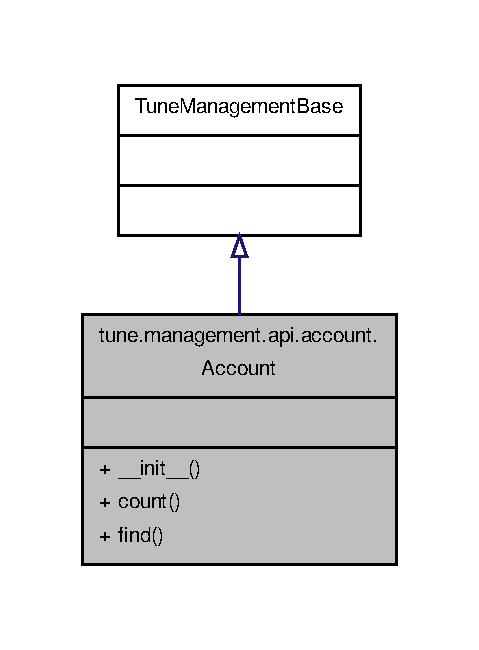
\includegraphics[width=230pt]{classtune_1_1management_1_1api_1_1account_1_1Account__inherit__graph}
\end{center}
\end{figure}


Collaboration diagram for tune.\-management.\-api.\-account.\-Account\-:
\nopagebreak
\begin{figure}[H]
\begin{center}
\leavevmode
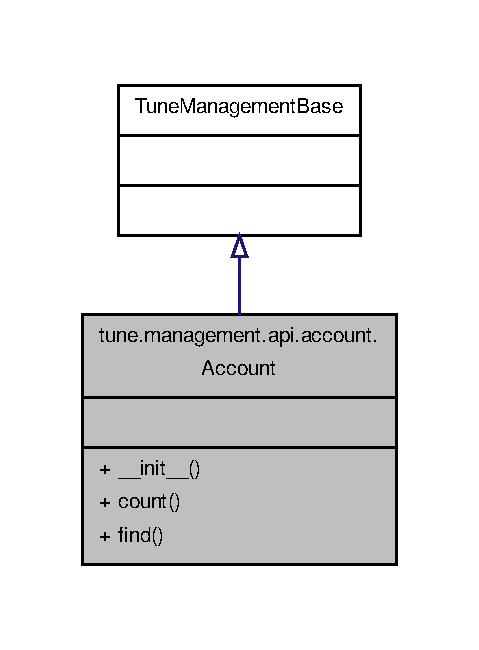
\includegraphics[width=230pt]{classtune_1_1management_1_1api_1_1account_1_1Account__coll__graph}
\end{center}
\end{figure}
\subsection*{Public Member Functions}
\begin{DoxyCompactItemize}
\item 
def \hyperlink{classtune_1_1management_1_1api_1_1account_1_1Account_a5dd49f5f497e7ffd0c5fdb6ca2c0a5c2}{\-\_\-\-\_\-init\-\_\-\-\_\-}
\begin{DoxyCompactList}\small\item\em The constructor. \end{DoxyCompactList}\item 
def \hyperlink{classtune_1_1management_1_1api_1_1account_1_1Account_a4a9a272db7dff634ea1e48df30a0b4f4}{count}
\begin{DoxyCompactList}\small\item\em Counts all existing records that match filter criteria. \end{DoxyCompactList}\item 
def \hyperlink{classtune_1_1management_1_1api_1_1account_1_1Account_af37c9d36cde138ff763e9a2b94b6218f}{find}
\begin{DoxyCompactList}\small\item\em Finds all existing records that match filter criteria and returns an array of found model data. \end{DoxyCompactList}\end{DoxyCompactItemize}


\subsection{Detailed Description}
Endpoint '/account'. 

Tune Management A\-P\-I endpoint '/account/' 

Definition at line 55 of file \-\_\-\-\_\-init\-\_\-\-\_\-.\-py.



\subsection{Constructor \& Destructor Documentation}
\hypertarget{classtune_1_1management_1_1api_1_1account_1_1Account_a5dd49f5f497e7ffd0c5fdb6ca2c0a5c2}{\index{tune\-::management\-::api\-::account\-::\-Account@{tune\-::management\-::api\-::account\-::\-Account}!\-\_\-\-\_\-init\-\_\-\-\_\-@{\-\_\-\-\_\-init\-\_\-\-\_\-}}
\index{\-\_\-\-\_\-init\-\_\-\-\_\-@{\-\_\-\-\_\-init\-\_\-\-\_\-}!tune::management::api::account::Account@{tune\-::management\-::api\-::account\-::\-Account}}
\subsubsection[{\-\_\-\-\_\-init\-\_\-\-\_\-}]{\setlength{\rightskip}{0pt plus 5cm}def tune.\-management.\-api.\-account.\-Account.\-\_\-\-\_\-init\-\_\-\-\_\- (
\begin{DoxyParamCaption}
\item[{}]{self, }
\item[{}]{api\-\_\-key, }
\item[{}]{validate = {\ttfamily False}}
\end{DoxyParamCaption}
)}}\label{classtune_1_1management_1_1api_1_1account_1_1Account_a5dd49f5f497e7ffd0c5fdb6ca2c0a5c2}


The constructor. 


\begin{DoxyParams}{Parameters}
{\em str} & api\-\_\-key Mobile\-App\-Tracking A\-P\-I Key. \\
\hline
{\em bool} & validate Validate fields used by actions. \\
\hline
\end{DoxyParams}


Definition at line 66 of file \-\_\-\-\_\-init\-\_\-\-\_\-.\-py.


\begin{DoxyCode}
66 
67         ):
68         TuneManagementBase.\_\_init\_\_(self, \textcolor{stringliteral}{"account"}, api\_key, validate)

\end{DoxyCode}


\subsection{Member Function Documentation}
\hypertarget{classtune_1_1management_1_1api_1_1account_1_1Account_a4a9a272db7dff634ea1e48df30a0b4f4}{\index{tune\-::management\-::api\-::account\-::\-Account@{tune\-::management\-::api\-::account\-::\-Account}!count@{count}}
\index{count@{count}!tune::management::api::account::Account@{tune\-::management\-::api\-::account\-::\-Account}}
\subsubsection[{count}]{\setlength{\rightskip}{0pt plus 5cm}def tune.\-management.\-api.\-account.\-Account.\-count (
\begin{DoxyParamCaption}
\item[{}]{self, }
\item[{}]{filter = {\ttfamily None}}
\end{DoxyParamCaption}
)}}\label{classtune_1_1management_1_1api_1_1account_1_1Account_a4a9a272db7dff634ea1e48df30a0b4f4}


Counts all existing records that match filter criteria. 


\begin{DoxyParams}{Parameters}
{\em string} & filter Filter the results and apply conditions\\
\hline
\end{DoxyParams}
Count accounts based upon provided constraints. 

Definition at line 75 of file \-\_\-\-\_\-init\-\_\-\-\_\-.\-py.


\begin{DoxyCode}
75 
76     \textcolor{keyword}{def }\hyperlink{classtune_1_1management_1_1api_1_1account_1_1Account_a4a9a272db7dff634ea1e48df30a0b4f4}{count}(self, filter=None):
77         \textcolor{keywordflow}{return} TuneManagementBase.call(
78             self,
79             action=\textcolor{stringliteral}{"count"},
80             query\_string\_dict=\{
81                 \textcolor{stringliteral}{'filter'}: filter
82             \}
83         )

\end{DoxyCode}


Here is the call graph for this function\-:
\nopagebreak
\begin{figure}[H]
\begin{center}
\leavevmode
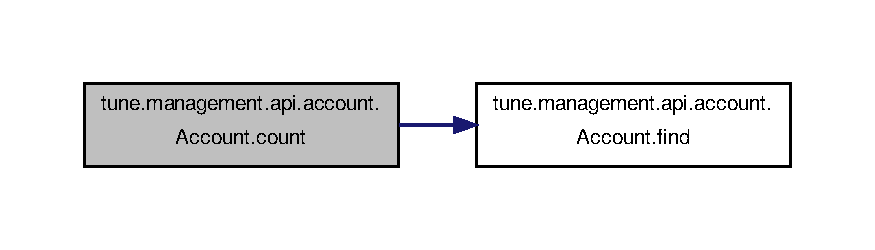
\includegraphics[width=350pt]{classtune_1_1management_1_1api_1_1account_1_1Account_a4a9a272db7dff634ea1e48df30a0b4f4_cgraph}
\end{center}
\end{figure}




Here is the caller graph for this function\-:
\nopagebreak
\begin{figure}[H]
\begin{center}
\leavevmode
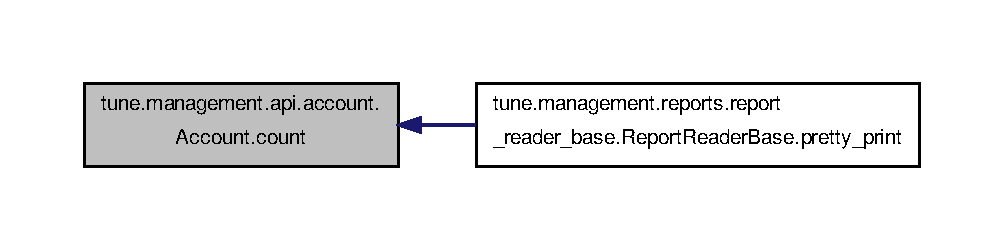
\includegraphics[width=350pt]{classtune_1_1management_1_1api_1_1account_1_1Account_a4a9a272db7dff634ea1e48df30a0b4f4_icgraph}
\end{center}
\end{figure}


\hypertarget{classtune_1_1management_1_1api_1_1account_1_1Account_af37c9d36cde138ff763e9a2b94b6218f}{\index{tune\-::management\-::api\-::account\-::\-Account@{tune\-::management\-::api\-::account\-::\-Account}!find@{find}}
\index{find@{find}!tune::management::api::account::Account@{tune\-::management\-::api\-::account\-::\-Account}}
\subsubsection[{find}]{\setlength{\rightskip}{0pt plus 5cm}def tune.\-management.\-api.\-account.\-Account.\-find (
\begin{DoxyParamCaption}
\item[{}]{self, }
\item[{}]{fields = {\ttfamily None}, }
\item[{}]{limit = {\ttfamily None}, }
\item[{}]{filter = {\ttfamily None}, }
\item[{}]{page = {\ttfamily None}, }
\item[{}]{sort = {\ttfamily None}}
\end{DoxyParamCaption}
)}}\label{classtune_1_1management_1_1api_1_1account_1_1Account_af37c9d36cde138ff763e9a2b94b6218f}


Finds all existing records that match filter criteria and returns an array of found model data. 


\begin{DoxyParams}{Parameters}
{\em string} & filter Filter the results and apply conditions that must be met for records to be included in data. \\
\hline
{\em string} & fields No value returns default fields, \char`\"{}\#  \char`\"{} returns all available fields, or provide specific fields. \\
\hline
{\em int} & limit Limit number of results, default 10, 0 shows all. \\
\hline
{\em int} & page Pagination, default 1. \\
\hline
{\em dict} & sort Expression defining sorting found records in result set base upon provided fields and its modifier (A\-S\-C or D\-E\-S\-C).\\
\hline
\end{DoxyParams}
\begin{DoxyReturn}{Returns}
object
\end{DoxyReturn}
Find accounts based upon provided constraints. 

Definition at line 110 of file \-\_\-\-\_\-init\-\_\-\-\_\-.\-py.


\begin{DoxyCode}
110 
111         ):
112         \textcolor{keywordflow}{return} TuneManagementBase.call(
113             self,
114             action=\textcolor{stringliteral}{"find"},
115             query\_string\_dict=\{
116                 \textcolor{stringliteral}{'fields'}: fields,
117                 \textcolor{stringliteral}{'filter'}: filter,
118                 \textcolor{stringliteral}{'limit'}: limit,
119                 \textcolor{stringliteral}{'page'}: page,
120                 \textcolor{stringliteral}{'sort'}: sort
121             \}
122         )
\end{DoxyCode}


Here is the caller graph for this function\-:
\nopagebreak
\begin{figure}[H]
\begin{center}
\leavevmode
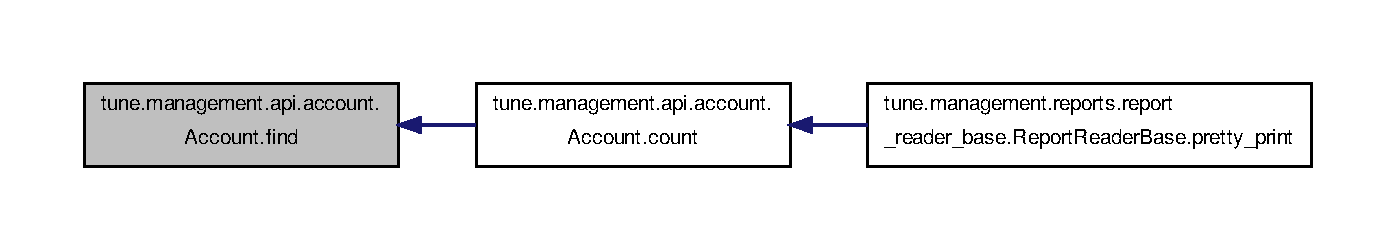
\includegraphics[width=350pt]{classtune_1_1management_1_1api_1_1account_1_1Account_af37c9d36cde138ff763e9a2b94b6218f_icgraph}
\end{center}
\end{figure}




The documentation for this class was generated from the following file\-:\begin{DoxyCompactItemize}
\item 
tune/management/api/account/\hyperlink{management_2api_2account_2____init_____8py}{\-\_\-\-\_\-init\-\_\-\-\_\-.\-py}\end{DoxyCompactItemize}

\hypertarget{classtune_1_1management_1_1api_1_1advertiser_1_1Advertiser}{\section{tune.\-management.\-api.\-advertiser.\-Advertiser Class Reference}
\label{classtune_1_1management_1_1api_1_1advertiser_1_1Advertiser}\index{tune.\-management.\-api.\-advertiser.\-Advertiser@{tune.\-management.\-api.\-advertiser.\-Advertiser}}
}


Endpoint '/advertisers'.  




Inheritance diagram for tune.\-management.\-api.\-advertiser.\-Advertiser\-:
\nopagebreak
\begin{figure}[H]
\begin{center}
\leavevmode
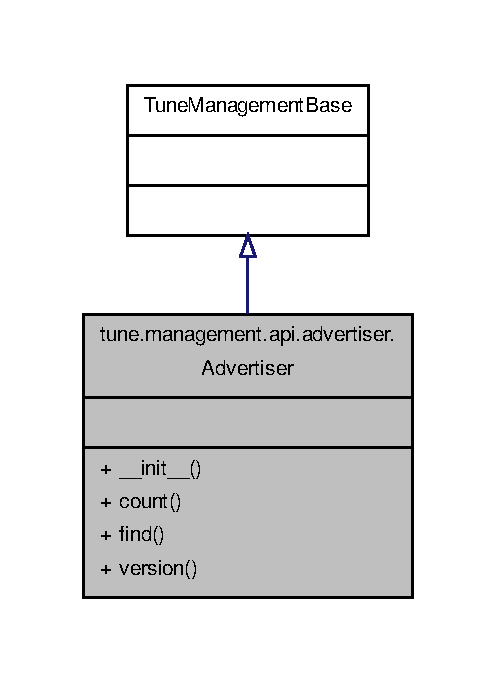
\includegraphics[width=238pt]{classtune_1_1management_1_1api_1_1advertiser_1_1Advertiser__inherit__graph}
\end{center}
\end{figure}


Collaboration diagram for tune.\-management.\-api.\-advertiser.\-Advertiser\-:
\nopagebreak
\begin{figure}[H]
\begin{center}
\leavevmode
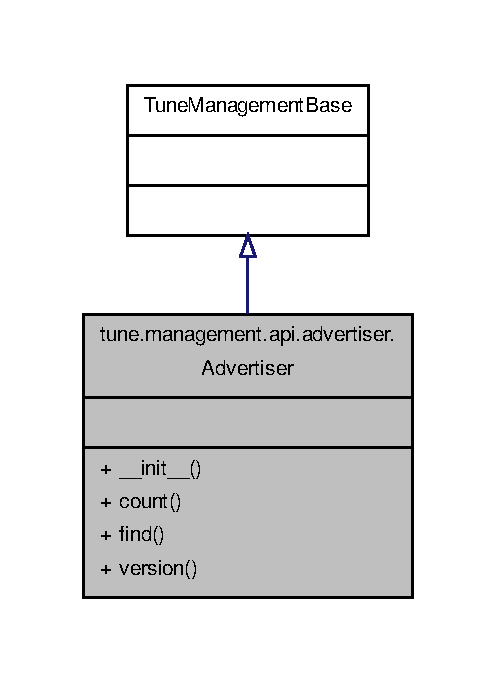
\includegraphics[width=238pt]{classtune_1_1management_1_1api_1_1advertiser_1_1Advertiser__coll__graph}
\end{center}
\end{figure}
\subsection*{Public Member Functions}
\begin{DoxyCompactItemize}
\item 
def \hyperlink{classtune_1_1management_1_1api_1_1advertiser_1_1Advertiser_a47b225259643daa567a8cf872b6af878}{\-\_\-\-\_\-init\-\_\-\-\_\-}
\begin{DoxyCompactList}\small\item\em The constructor. \end{DoxyCompactList}\item 
def \hyperlink{classtune_1_1management_1_1api_1_1advertiser_1_1Advertiser_a797fdee675b686bd1e3b0b9b3bcb6b98}{count}
\begin{DoxyCompactList}\small\item\em Counts all existing records that match filter criteria. \end{DoxyCompactList}\item 
def \hyperlink{classtune_1_1management_1_1api_1_1advertiser_1_1Advertiser_a758ffc0ead470458c29a5e3da342cfd7}{find}
\begin{DoxyCompactList}\small\item\em Finds all existing records that match filter criteria and returns an array of found model data. \end{DoxyCompactList}\end{DoxyCompactItemize}
\subsection*{Static Public Member Functions}
\begin{DoxyCompactItemize}
\item 
def \hyperlink{classtune_1_1management_1_1api_1_1advertiser_1_1Advertiser_a930b9245bf74b54deff8d6cd64aa37f4}{version}
\end{DoxyCompactItemize}


\subsection{Detailed Description}
Endpoint '/advertisers'. 

Tune Management A\-P\-I endpoint '/advertiser/' 

Definition at line 65 of file \-\_\-\-\_\-init\-\_\-\-\_\-.\-py.



\subsection{Constructor \& Destructor Documentation}
\hypertarget{classtune_1_1management_1_1api_1_1advertiser_1_1Advertiser_a47b225259643daa567a8cf872b6af878}{\index{tune\-::management\-::api\-::advertiser\-::\-Advertiser@{tune\-::management\-::api\-::advertiser\-::\-Advertiser}!\-\_\-\-\_\-init\-\_\-\-\_\-@{\-\_\-\-\_\-init\-\_\-\-\_\-}}
\index{\-\_\-\-\_\-init\-\_\-\-\_\-@{\-\_\-\-\_\-init\-\_\-\-\_\-}!tune::management::api::advertiser::Advertiser@{tune\-::management\-::api\-::advertiser\-::\-Advertiser}}
\subsubsection[{\-\_\-\-\_\-init\-\_\-\-\_\-}]{\setlength{\rightskip}{0pt plus 5cm}def tune.\-management.\-api.\-advertiser.\-Advertiser.\-\_\-\-\_\-init\-\_\-\-\_\- (
\begin{DoxyParamCaption}
\item[{}]{self, }
\item[{}]{api\-\_\-key, }
\item[{}]{validate = {\ttfamily False}}
\end{DoxyParamCaption}
)}}\label{classtune_1_1management_1_1api_1_1advertiser_1_1Advertiser_a47b225259643daa567a8cf872b6af878}


The constructor. 


\begin{DoxyParams}{Parameters}
{\em str} & api\-\_\-key Mobile\-App\-Tracking A\-P\-I Key. \\
\hline
{\em bool} & validate Validate fields used by actions. \\
\hline
\end{DoxyParams}


Definition at line 76 of file \-\_\-\-\_\-init\-\_\-\-\_\-.\-py.


\begin{DoxyCode}
76 
77         ):
78         TuneManagementBase.\_\_init\_\_(self, \textcolor{stringliteral}{"account"}, api\_key, validate)

\end{DoxyCode}


Here is the call graph for this function\-:
\nopagebreak
\begin{figure}[H]
\begin{center}
\leavevmode
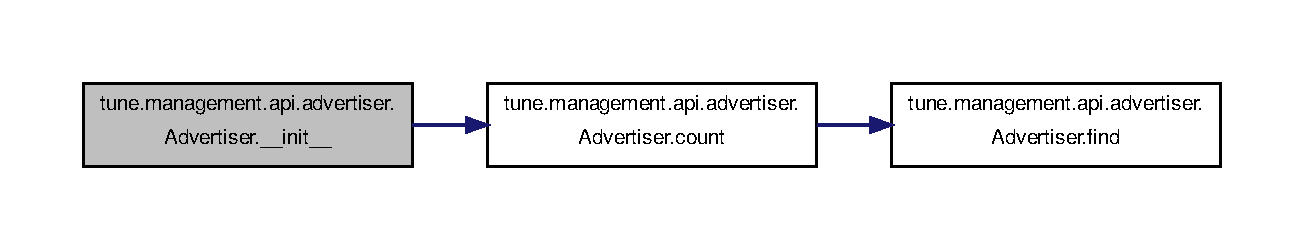
\includegraphics[width=350pt]{classtune_1_1management_1_1api_1_1advertiser_1_1Advertiser_a47b225259643daa567a8cf872b6af878_cgraph}
\end{center}
\end{figure}




\subsection{Member Function Documentation}
\hypertarget{classtune_1_1management_1_1api_1_1advertiser_1_1Advertiser_a797fdee675b686bd1e3b0b9b3bcb6b98}{\index{tune\-::management\-::api\-::advertiser\-::\-Advertiser@{tune\-::management\-::api\-::advertiser\-::\-Advertiser}!count@{count}}
\index{count@{count}!tune::management::api::advertiser::Advertiser@{tune\-::management\-::api\-::advertiser\-::\-Advertiser}}
\subsubsection[{count}]{\setlength{\rightskip}{0pt plus 5cm}def tune.\-management.\-api.\-advertiser.\-Advertiser.\-count (
\begin{DoxyParamCaption}
\item[{}]{self, }
\item[{}]{filter = {\ttfamily None}}
\end{DoxyParamCaption}
)}}\label{classtune_1_1management_1_1api_1_1advertiser_1_1Advertiser_a797fdee675b686bd1e3b0b9b3bcb6b98}


Counts all existing records that match filter criteria. 


\begin{DoxyParams}{Parameters}
{\em string} & filter Filter the results and apply conditions that must be met for records to be included in data.\\
\hline
\end{DoxyParams}
Count advertisers based upon provided constraints. 

Definition at line 88 of file \-\_\-\-\_\-init\-\_\-\-\_\-.\-py.


\begin{DoxyCode}
88 
89         ):
90         \textcolor{keywordflow}{return} TuneManagementBase.call(
91             self,
92             action=\textcolor{stringliteral}{"count"},
93             query\_string\_dict=\{
94                 \textcolor{stringliteral}{'filter'}: filter
95             \}
96         )

\end{DoxyCode}


Here is the call graph for this function\-:
\nopagebreak
\begin{figure}[H]
\begin{center}
\leavevmode
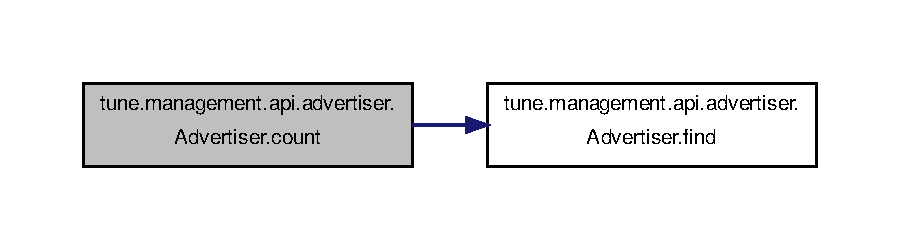
\includegraphics[width=350pt]{classtune_1_1management_1_1api_1_1advertiser_1_1Advertiser_a797fdee675b686bd1e3b0b9b3bcb6b98_cgraph}
\end{center}
\end{figure}




Here is the caller graph for this function\-:
\nopagebreak
\begin{figure}[H]
\begin{center}
\leavevmode
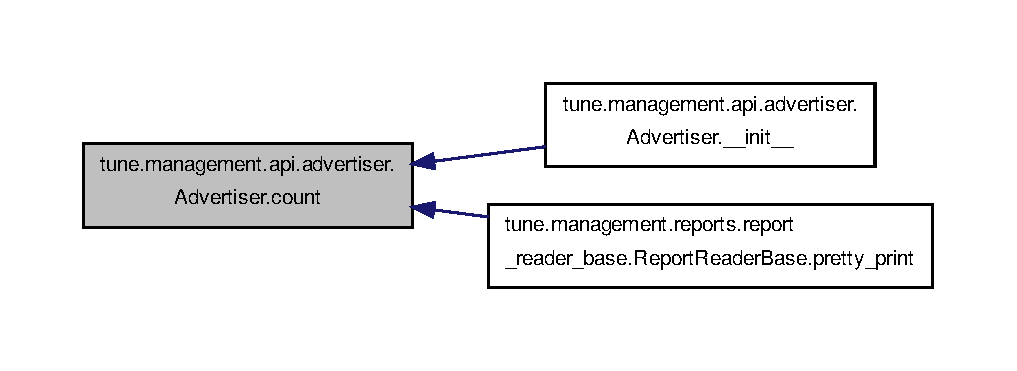
\includegraphics[width=350pt]{classtune_1_1management_1_1api_1_1advertiser_1_1Advertiser_a797fdee675b686bd1e3b0b9b3bcb6b98_icgraph}
\end{center}
\end{figure}


\hypertarget{classtune_1_1management_1_1api_1_1advertiser_1_1Advertiser_a758ffc0ead470458c29a5e3da342cfd7}{\index{tune\-::management\-::api\-::advertiser\-::\-Advertiser@{tune\-::management\-::api\-::advertiser\-::\-Advertiser}!find@{find}}
\index{find@{find}!tune::management::api::advertiser::Advertiser@{tune\-::management\-::api\-::advertiser\-::\-Advertiser}}
\subsubsection[{find}]{\setlength{\rightskip}{0pt plus 5cm}def tune.\-management.\-api.\-advertiser.\-Advertiser.\-find (
\begin{DoxyParamCaption}
\item[{}]{self, }
\item[{}]{fields = {\ttfamily None}, }
\item[{}]{filter = {\ttfamily None}, }
\item[{}]{limit = {\ttfamily None}, }
\item[{}]{page = {\ttfamily None}, }
\item[{}]{sort = {\ttfamily None}}
\end{DoxyParamCaption}
)}}\label{classtune_1_1management_1_1api_1_1advertiser_1_1Advertiser_a758ffc0ead470458c29a5e3da342cfd7}


Finds all existing records that match filter criteria and returns an array of found model data. 


\begin{DoxyParams}{Parameters}
{\em string} & filter Filter the results and apply conditions that must be met for records to be included in data. \\
\hline
{\em string} & fields No value returns default fields, \char`\"{}\#  \char`\"{} returns all available fields, or provide specific fields. \\
\hline
{\em int} & limit Limit number of results, default 10, 0 shows all. \\
\hline
{\em int} & page Pagination, default 1. \\
\hline
{\em dict} & sort Expression defining sorting found records in result set base upon provided fields and its modifier (A\-S\-C or D\-E\-S\-C).\\
\hline
\end{DoxyParams}
\begin{DoxyReturn}{Returns}
object 
\end{DoxyReturn}
\begin{DoxySeeAlso}{See Also}
Response
\end{DoxySeeAlso}
Find advertisers based upon provided constraints. 

Definition at line 123 of file \-\_\-\-\_\-init\-\_\-\-\_\-.\-py.


\begin{DoxyCode}
123 
124         ):
125         \textcolor{keywordflow}{return} TuneManagementBase.call(
126             self,
127             action=\textcolor{stringliteral}{"find"},
128             query\_string\_dict=\{
129                 \textcolor{stringliteral}{'fields'}: fields,
130                 \textcolor{stringliteral}{'filter'}: filter,
131                 \textcolor{stringliteral}{'limit'}: limit,
132                 \textcolor{stringliteral}{'page'}: page,
133                 \textcolor{stringliteral}{'sort'}: sort
134             \}
135         )

\end{DoxyCode}


Here is the caller graph for this function\-:
\nopagebreak
\begin{figure}[H]
\begin{center}
\leavevmode
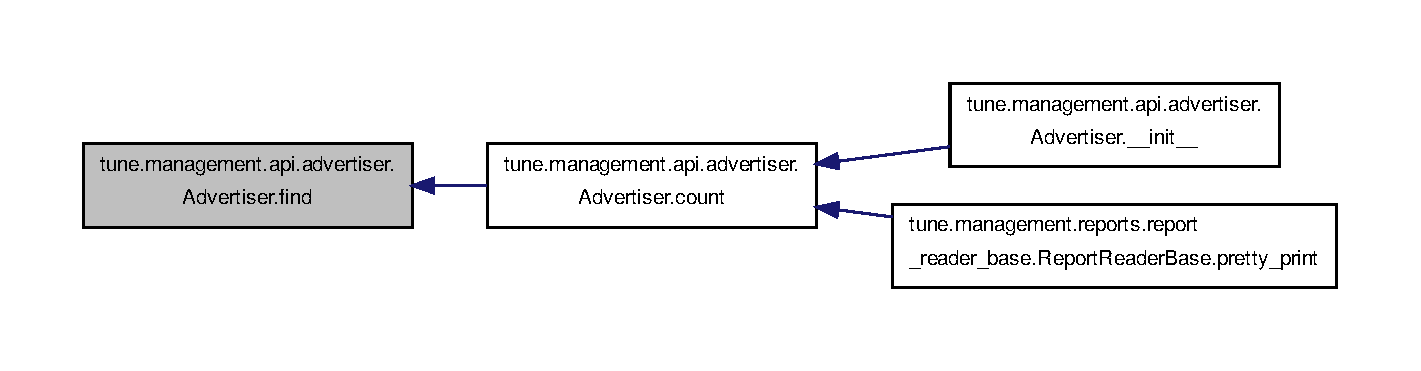
\includegraphics[width=350pt]{classtune_1_1management_1_1api_1_1advertiser_1_1Advertiser_a758ffc0ead470458c29a5e3da342cfd7_icgraph}
\end{center}
\end{figure}


\hypertarget{classtune_1_1management_1_1api_1_1advertiser_1_1Advertiser_a930b9245bf74b54deff8d6cd64aa37f4}{\index{tune\-::management\-::api\-::advertiser\-::\-Advertiser@{tune\-::management\-::api\-::advertiser\-::\-Advertiser}!version@{version}}
\index{version@{version}!tune::management::api::advertiser::Advertiser@{tune\-::management\-::api\-::advertiser\-::\-Advertiser}}
\subsubsection[{version}]{\setlength{\rightskip}{0pt plus 5cm}def tune.\-management.\-api.\-advertiser.\-Advertiser.\-version (
\begin{DoxyParamCaption}
{}
\end{DoxyParamCaption}
)\hspace{0.3cm}{\ttfamily [static]}}}\label{classtune_1_1management_1_1api_1_1advertiser_1_1Advertiser_a930b9245bf74b54deff8d6cd64aa37f4}


Definition at line 137 of file \-\_\-\-\_\-init\-\_\-\-\_\-.\-py.


\begin{DoxyCode}
137 
138     \textcolor{keyword}{def }\hyperlink{classtune_1_1management_1_1api_1_1advertiser_1_1Advertiser_a930b9245bf74b54deff8d6cd64aa37f4}{version}():
139         \textcolor{keywordflow}{return} TuneManagementBase.version()
\end{DoxyCode}


The documentation for this class was generated from the following file\-:\begin{DoxyCompactItemize}
\item 
tune/management/api/advertiser/\hyperlink{management_2api_2advertiser_2____init_____8py}{\-\_\-\-\_\-init\-\_\-\-\_\-.\-py}\end{DoxyCompactItemize}

\hypertarget{classtune_1_1management_1_1api_1_1advertiser_1_1stats_1_1clicks_1_1Clicks}{\section{tune.\-management.\-api.\-advertiser.\-stats.\-clicks.\-Clicks Class Reference}
\label{classtune_1_1management_1_1api_1_1advertiser_1_1stats_1_1clicks_1_1Clicks}\index{tune.\-management.\-api.\-advertiser.\-stats.\-clicks.\-Clicks@{tune.\-management.\-api.\-advertiser.\-stats.\-clicks.\-Clicks}}
}


Inheritance diagram for tune.\-management.\-api.\-advertiser.\-stats.\-clicks.\-Clicks\-:
\nopagebreak
\begin{figure}[H]
\begin{center}
\leavevmode
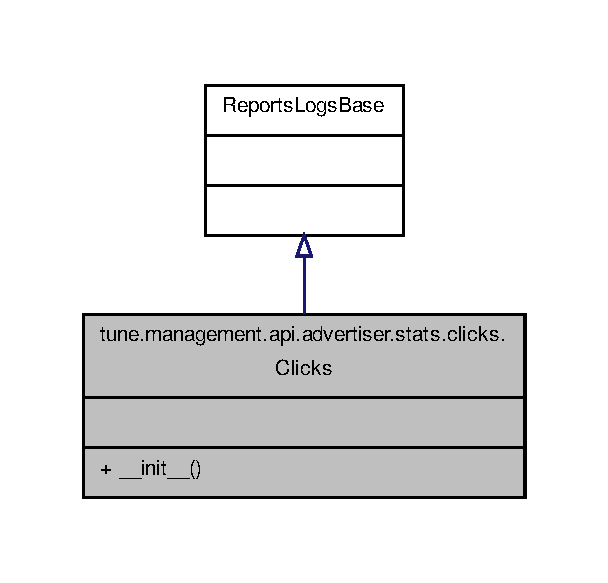
\includegraphics[width=292pt]{classtune_1_1management_1_1api_1_1advertiser_1_1stats_1_1clicks_1_1Clicks__inherit__graph}
\end{center}
\end{figure}


Collaboration diagram for tune.\-management.\-api.\-advertiser.\-stats.\-clicks.\-Clicks\-:
\nopagebreak
\begin{figure}[H]
\begin{center}
\leavevmode
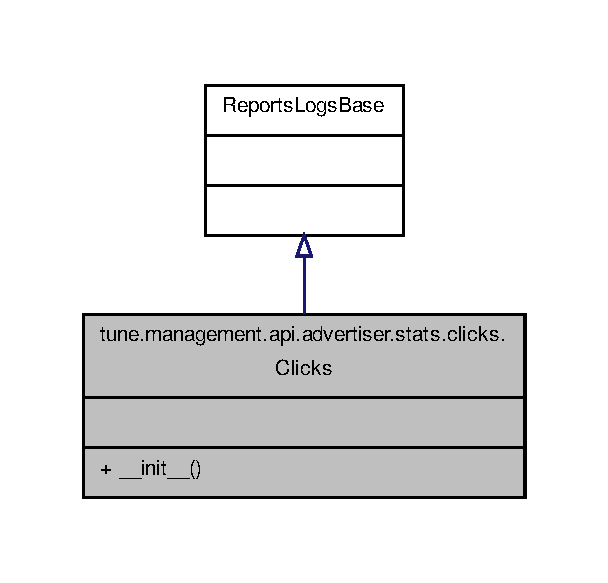
\includegraphics[width=292pt]{classtune_1_1management_1_1api_1_1advertiser_1_1stats_1_1clicks_1_1Clicks__coll__graph}
\end{center}
\end{figure}
\subsection*{Public Member Functions}
\begin{DoxyCompactItemize}
\item 
def \hyperlink{classtune_1_1management_1_1api_1_1advertiser_1_1stats_1_1clicks_1_1Clicks_a730985abef7492c713af38c105aa224f}{\-\_\-\-\_\-init\-\_\-\-\_\-}
\begin{DoxyCompactList}\small\item\em The constructor. \end{DoxyCompactList}\end{DoxyCompactItemize}


\subsection{Detailed Description}


Definition at line 55 of file clicks.\-py.



\subsection{Constructor \& Destructor Documentation}
\hypertarget{classtune_1_1management_1_1api_1_1advertiser_1_1stats_1_1clicks_1_1Clicks_a730985abef7492c713af38c105aa224f}{\index{tune\-::management\-::api\-::advertiser\-::stats\-::clicks\-::\-Clicks@{tune\-::management\-::api\-::advertiser\-::stats\-::clicks\-::\-Clicks}!\-\_\-\-\_\-init\-\_\-\-\_\-@{\-\_\-\-\_\-init\-\_\-\-\_\-}}
\index{\-\_\-\-\_\-init\-\_\-\-\_\-@{\-\_\-\-\_\-init\-\_\-\-\_\-}!tune::management::api::advertiser::stats::clicks::Clicks@{tune\-::management\-::api\-::advertiser\-::stats\-::clicks\-::\-Clicks}}
\subsubsection[{\-\_\-\-\_\-init\-\_\-\-\_\-}]{\setlength{\rightskip}{0pt plus 5cm}def tune.\-management.\-api.\-advertiser.\-stats.\-clicks.\-Clicks.\-\_\-\-\_\-init\-\_\-\-\_\- (
\begin{DoxyParamCaption}
\item[{}]{self, }
\item[{}]{api\-\_\-key, }
\item[{}]{validate = {\ttfamily False}}
\end{DoxyParamCaption}
)}}\label{classtune_1_1management_1_1api_1_1advertiser_1_1stats_1_1clicks_1_1Clicks_a730985abef7492c713af38c105aa224f}


The constructor. 


\begin{DoxyParams}{Parameters}
{\em str} & api\-\_\-key Mobile\-App\-Tracking A\-P\-I Key. \\
\hline
{\em bool} & validate Validate fields used by actions. \\
\hline
\end{DoxyParams}


Definition at line 66 of file clicks.\-py.


\begin{DoxyCode}
66 
67         ):
68         ReportsLogsBase.\_\_init\_\_(
69             self,
70             \textcolor{stringliteral}{"advertiser/stats/clicks"},
71             api\_key,
72             \textcolor{keyword}{True},
73             \textcolor{keyword}{True},
74             validate
75         )
\end{DoxyCode}


The documentation for this class was generated from the following file\-:\begin{DoxyCompactItemize}
\item 
tune/management/api/advertiser/stats/\hyperlink{clicks_8py}{clicks.\-py}\end{DoxyCompactItemize}

\hypertarget{classtune_1_1management_1_1api_1_1advertiser_1_1stats_1_1event__items_1_1EventItems}{\section{tune.\-management.\-api.\-advertiser.\-stats.\-event\-\_\-items.\-Event\-Items Class Reference}
\label{classtune_1_1management_1_1api_1_1advertiser_1_1stats_1_1event__items_1_1EventItems}\index{tune.\-management.\-api.\-advertiser.\-stats.\-event\-\_\-items.\-Event\-Items@{tune.\-management.\-api.\-advertiser.\-stats.\-event\-\_\-items.\-Event\-Items}}
}


Inheritance diagram for tune.\-management.\-api.\-advertiser.\-stats.\-event\-\_\-items.\-Event\-Items\-:
\nopagebreak
\begin{figure}[H]
\begin{center}
\leavevmode
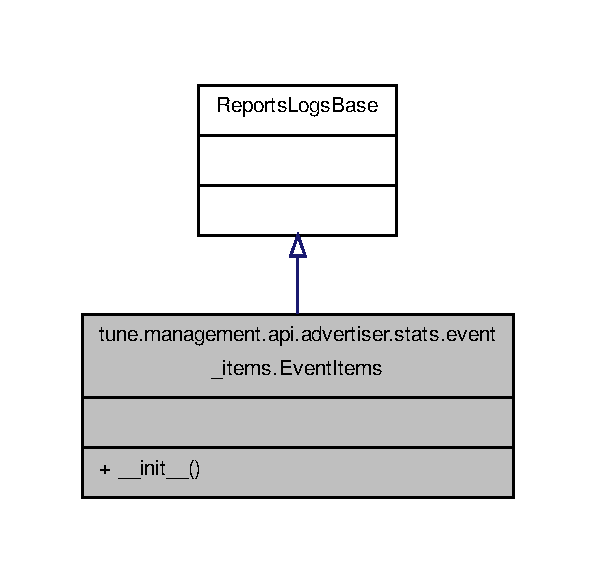
\includegraphics[width=286pt]{classtune_1_1management_1_1api_1_1advertiser_1_1stats_1_1event__items_1_1EventItems__inherit__graph}
\end{center}
\end{figure}


Collaboration diagram for tune.\-management.\-api.\-advertiser.\-stats.\-event\-\_\-items.\-Event\-Items\-:
\nopagebreak
\begin{figure}[H]
\begin{center}
\leavevmode
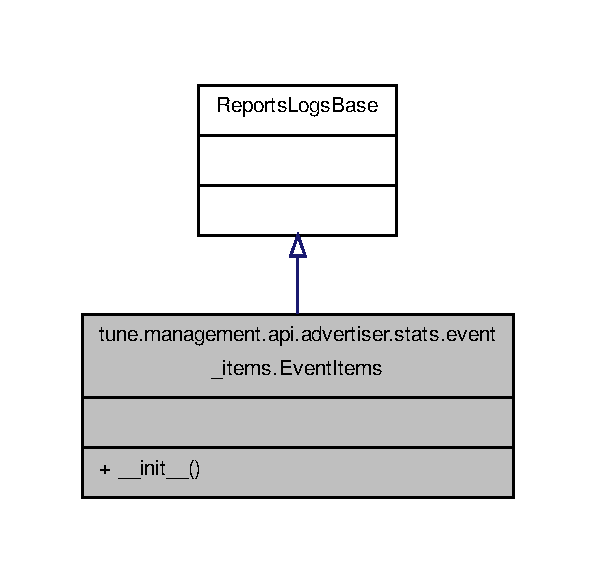
\includegraphics[width=286pt]{classtune_1_1management_1_1api_1_1advertiser_1_1stats_1_1event__items_1_1EventItems__coll__graph}
\end{center}
\end{figure}
\subsection*{Public Member Functions}
\begin{DoxyCompactItemize}
\item 
def \hyperlink{classtune_1_1management_1_1api_1_1advertiser_1_1stats_1_1event__items_1_1EventItems_aa5989b22c37e1bbe7ae8d12d1d3d9a87}{\-\_\-\-\_\-init\-\_\-\-\_\-}
\begin{DoxyCompactList}\small\item\em The constructor. \end{DoxyCompactList}\end{DoxyCompactItemize}


\subsection{Detailed Description}


Definition at line 51 of file event\-\_\-items.\-py.



\subsection{Constructor \& Destructor Documentation}
\hypertarget{classtune_1_1management_1_1api_1_1advertiser_1_1stats_1_1event__items_1_1EventItems_aa5989b22c37e1bbe7ae8d12d1d3d9a87}{\index{tune\-::management\-::api\-::advertiser\-::stats\-::event\-\_\-items\-::\-Event\-Items@{tune\-::management\-::api\-::advertiser\-::stats\-::event\-\_\-items\-::\-Event\-Items}!\-\_\-\-\_\-init\-\_\-\-\_\-@{\-\_\-\-\_\-init\-\_\-\-\_\-}}
\index{\-\_\-\-\_\-init\-\_\-\-\_\-@{\-\_\-\-\_\-init\-\_\-\-\_\-}!tune::management::api::advertiser::stats::event_items::EventItems@{tune\-::management\-::api\-::advertiser\-::stats\-::event\-\_\-items\-::\-Event\-Items}}
\subsubsection[{\-\_\-\-\_\-init\-\_\-\-\_\-}]{\setlength{\rightskip}{0pt plus 5cm}def tune.\-management.\-api.\-advertiser.\-stats.\-event\-\_\-items.\-Event\-Items.\-\_\-\-\_\-init\-\_\-\-\_\- (
\begin{DoxyParamCaption}
\item[{}]{self, }
\item[{}]{api\-\_\-key, }
\item[{}]{validate = {\ttfamily False}}
\end{DoxyParamCaption}
)}}\label{classtune_1_1management_1_1api_1_1advertiser_1_1stats_1_1event__items_1_1EventItems_aa5989b22c37e1bbe7ae8d12d1d3d9a87}


The constructor. 


\begin{DoxyParams}{Parameters}
{\em str} & api\-\_\-key Mobile\-App\-Tracking A\-P\-I Key. \\
\hline
{\em bool} & validate Validate fields used by actions. \\
\hline
\end{DoxyParams}


Definition at line 62 of file event\-\_\-items.\-py.


\begin{DoxyCode}
62 
63         ):
64         ReportsLogsBase.\_\_init\_\_(
65             self,
66             \textcolor{stringliteral}{"advertiser/stats/event/items"},
67             api\_key,
68             \textcolor{keyword}{False},
69             \textcolor{keyword}{True},
70             validate
71         )
\end{DoxyCode}


The documentation for this class was generated from the following file\-:\begin{DoxyCompactItemize}
\item 
tune/management/api/advertiser/stats/\hyperlink{event__items_8py}{event\-\_\-items.\-py}\end{DoxyCompactItemize}

\hypertarget{classtune_1_1management_1_1api_1_1advertiser_1_1stats_1_1events_1_1Events}{\section{tune.\-management.\-api.\-advertiser.\-stats.\-events.\-Events Class Reference}
\label{classtune_1_1management_1_1api_1_1advertiser_1_1stats_1_1events_1_1Events}\index{tune.\-management.\-api.\-advertiser.\-stats.\-events.\-Events@{tune.\-management.\-api.\-advertiser.\-stats.\-events.\-Events}}
}


Inheritance diagram for tune.\-management.\-api.\-advertiser.\-stats.\-events.\-Events\-:
\nopagebreak
\begin{figure}[H]
\begin{center}
\leavevmode
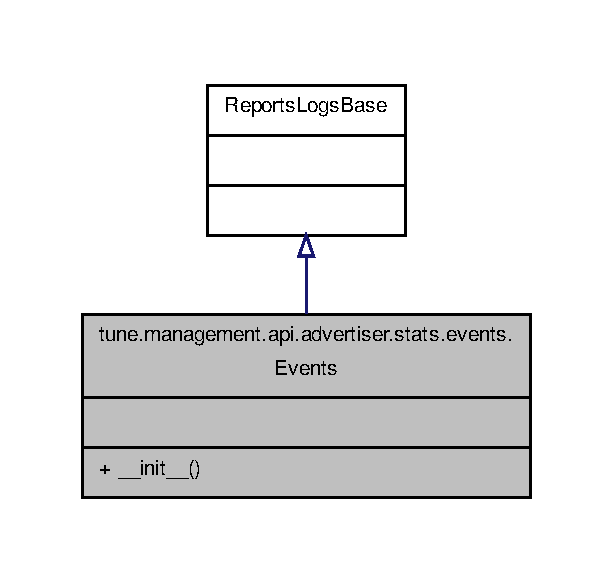
\includegraphics[width=294pt]{classtune_1_1management_1_1api_1_1advertiser_1_1stats_1_1events_1_1Events__inherit__graph}
\end{center}
\end{figure}


Collaboration diagram for tune.\-management.\-api.\-advertiser.\-stats.\-events.\-Events\-:
\nopagebreak
\begin{figure}[H]
\begin{center}
\leavevmode
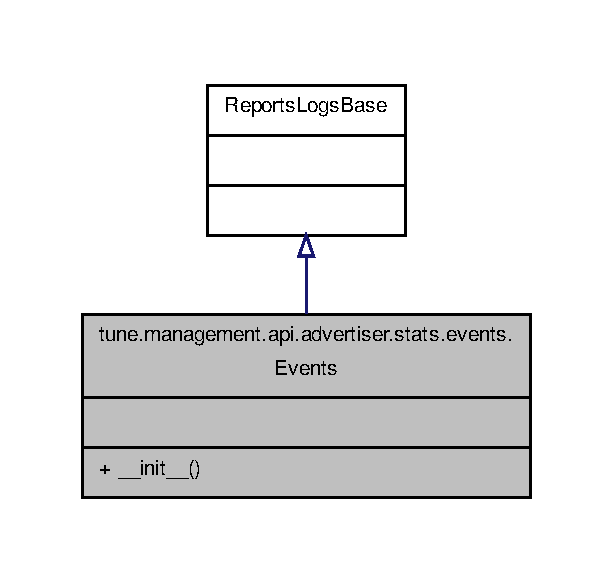
\includegraphics[width=294pt]{classtune_1_1management_1_1api_1_1advertiser_1_1stats_1_1events_1_1Events__coll__graph}
\end{center}
\end{figure}
\subsection*{Public Member Functions}
\begin{DoxyCompactItemize}
\item 
def \hyperlink{classtune_1_1management_1_1api_1_1advertiser_1_1stats_1_1events_1_1Events_ad5a3bc6a4fcf5cfaeee850847f5ad259}{\-\_\-\-\_\-init\-\_\-\-\_\-}
\begin{DoxyCompactList}\small\item\em The constructor. \end{DoxyCompactList}\end{DoxyCompactItemize}


\subsection{Detailed Description}


Definition at line 50 of file events.\-py.



\subsection{Constructor \& Destructor Documentation}
\hypertarget{classtune_1_1management_1_1api_1_1advertiser_1_1stats_1_1events_1_1Events_ad5a3bc6a4fcf5cfaeee850847f5ad259}{\index{tune\-::management\-::api\-::advertiser\-::stats\-::events\-::\-Events@{tune\-::management\-::api\-::advertiser\-::stats\-::events\-::\-Events}!\-\_\-\-\_\-init\-\_\-\-\_\-@{\-\_\-\-\_\-init\-\_\-\-\_\-}}
\index{\-\_\-\-\_\-init\-\_\-\-\_\-@{\-\_\-\-\_\-init\-\_\-\-\_\-}!tune::management::api::advertiser::stats::events::Events@{tune\-::management\-::api\-::advertiser\-::stats\-::events\-::\-Events}}
\subsubsection[{\-\_\-\-\_\-init\-\_\-\-\_\-}]{\setlength{\rightskip}{0pt plus 5cm}def tune.\-management.\-api.\-advertiser.\-stats.\-events.\-Events.\-\_\-\-\_\-init\-\_\-\-\_\- (
\begin{DoxyParamCaption}
\item[{}]{self, }
\item[{}]{api\-\_\-key, }
\item[{}]{validate = {\ttfamily False}}
\end{DoxyParamCaption}
)}}\label{classtune_1_1management_1_1api_1_1advertiser_1_1stats_1_1events_1_1Events_ad5a3bc6a4fcf5cfaeee850847f5ad259}


The constructor. 


\begin{DoxyParams}{Parameters}
{\em str} & api\-\_\-key Mobile\-App\-Tracking A\-P\-I Key. \\
\hline
{\em bool} & validate Validate fields used by actions. \\
\hline
\end{DoxyParams}


Definition at line 61 of file events.\-py.


\begin{DoxyCode}
61 
62         ):
63         ReportsLogsBase.\_\_init\_\_(
64             self,
65             \textcolor{stringliteral}{"advertiser/stats/events"},
66             api\_key,
67             \textcolor{keyword}{True},
68             \textcolor{keyword}{True},
69             validate
70         )
\end{DoxyCode}


The documentation for this class was generated from the following file\-:\begin{DoxyCompactItemize}
\item 
tune/management/api/advertiser/stats/\hyperlink{events_8py}{events.\-py}\end{DoxyCompactItemize}

\hypertarget{classException}{\section{Exception Class Reference}
\label{classException}\index{Exception@{Exception}}
}


Inheritance diagram for Exception\-:
\nopagebreak
\begin{figure}[H]
\begin{center}
\leavevmode
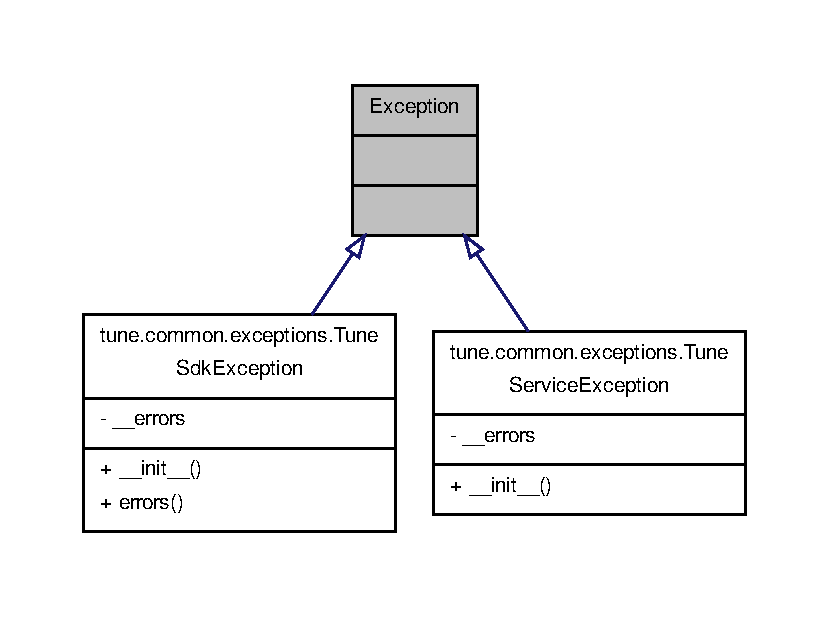
\includegraphics[width=350pt]{classException__inherit__graph}
\end{center}
\end{figure}


Collaboration diagram for Exception\-:
\nopagebreak
\begin{figure}[H]
\begin{center}
\leavevmode
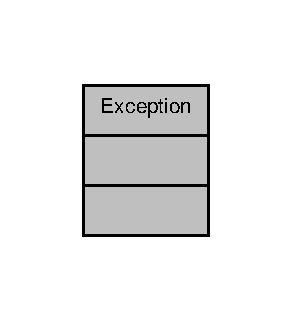
\includegraphics[width=140pt]{classException__coll__graph}
\end{center}
\end{figure}


The documentation for this class was generated from the following file\-:\begin{DoxyCompactItemize}
\item 
tune/common/\hyperlink{exceptions_8py}{exceptions.\-py}\end{DoxyCompactItemize}

\hypertarget{classtune_1_1management_1_1api_1_1export_1_1Export}{\section{tune.\-management.\-api.\-export.\-Export Class Reference}
\label{classtune_1_1management_1_1api_1_1export_1_1Export}\index{tune.\-management.\-api.\-export.\-Export@{tune.\-management.\-api.\-export.\-Export}}
}


/export  




Inheritance diagram for tune.\-management.\-api.\-export.\-Export\-:
\nopagebreak
\begin{figure}[H]
\begin{center}
\leavevmode
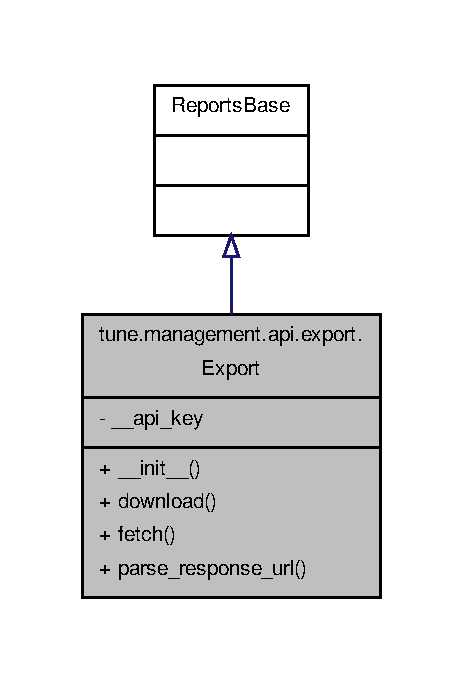
\includegraphics[width=222pt]{classtune_1_1management_1_1api_1_1export_1_1Export__inherit__graph}
\end{center}
\end{figure}


Collaboration diagram for tune.\-management.\-api.\-export.\-Export\-:
\nopagebreak
\begin{figure}[H]
\begin{center}
\leavevmode
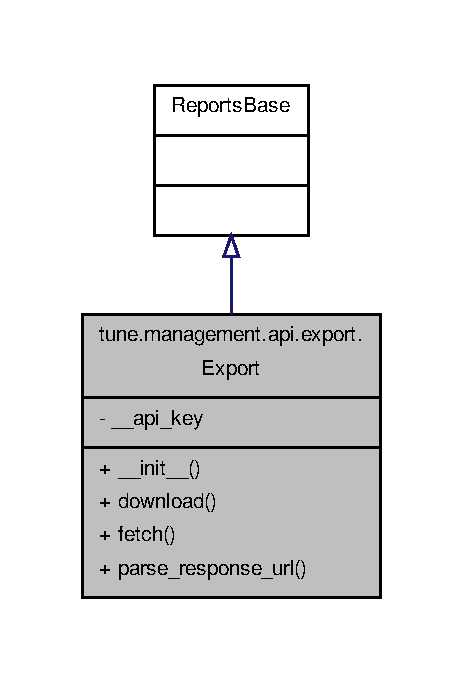
\includegraphics[width=222pt]{classtune_1_1management_1_1api_1_1export_1_1Export__coll__graph}
\end{center}
\end{figure}
\subsection*{Public Member Functions}
\begin{DoxyCompactItemize}
\item 
def \hyperlink{classtune_1_1management_1_1api_1_1export_1_1Export_a14c11f5e86025609ee4f1a02d190b038}{\-\_\-\-\_\-init\-\_\-\-\_\-}
\begin{DoxyCompactList}\small\item\em Constructor. \end{DoxyCompactList}\item 
def \hyperlink{classtune_1_1management_1_1api_1_1export_1_1Export_a7c8f4a974ae5d915feb57bc4c3502f93}{download}
\begin{DoxyCompactList}\small\item\em Request status from export queue for report. \end{DoxyCompactList}\item 
def \hyperlink{classtune_1_1management_1_1api_1_1export_1_1Export_af0819d2ba55d77f4f7f45ef5a91e1b96}{fetch}
\end{DoxyCompactItemize}
\subsection*{Static Public Member Functions}
\begin{DoxyCompactItemize}
\item 
def \hyperlink{classtune_1_1management_1_1api_1_1export_1_1Export_a39968f1bdbfdba59678de14db78c7ccc}{parse\-\_\-response\-\_\-url}
\begin{DoxyCompactList}\small\item\em Helper function for parsing export status response to gather report url. \end{DoxyCompactList}\end{DoxyCompactItemize}
\subsection*{Private Attributes}
\begin{DoxyCompactItemize}
\item 
\hyperlink{classtune_1_1management_1_1api_1_1export_1_1Export_ad9a517a5da2e72b2c26695151909ffe2}{\-\_\-\-\_\-api\-\_\-key}
\end{DoxyCompactItemize}


\subsection{Detailed Description}
/export 

Tune Management A\-P\-I controller '/export/'. 

Definition at line 49 of file export.\-py.



\subsection{Constructor \& Destructor Documentation}
\hypertarget{classtune_1_1management_1_1api_1_1export_1_1Export_a14c11f5e86025609ee4f1a02d190b038}{\index{tune\-::management\-::api\-::export\-::\-Export@{tune\-::management\-::api\-::export\-::\-Export}!\-\_\-\-\_\-init\-\_\-\-\_\-@{\-\_\-\-\_\-init\-\_\-\-\_\-}}
\index{\-\_\-\-\_\-init\-\_\-\-\_\-@{\-\_\-\-\_\-init\-\_\-\-\_\-}!tune::management::api::export::Export@{tune\-::management\-::api\-::export\-::\-Export}}
\subsubsection[{\-\_\-\-\_\-init\-\_\-\-\_\-}]{\setlength{\rightskip}{0pt plus 5cm}def tune.\-management.\-api.\-export.\-Export.\-\_\-\-\_\-init\-\_\-\-\_\- (
\begin{DoxyParamCaption}
\item[{}]{self, }
\item[{}]{api\-\_\-key}
\end{DoxyParamCaption}
)}}\label{classtune_1_1management_1_1api_1_1export_1_1Export_a14c11f5e86025609ee4f1a02d190b038}


Constructor. 


\begin{DoxyParams}{Parameters}
{\em str} & api\-\_\-key Tune Mobile\-App\-Tracking A\-P\-I Key \\
\hline
\end{DoxyParams}


Definition at line 53 of file export.\-py.


\begin{DoxyCode}
53 
54     \textcolor{keyword}{def }\hyperlink{classtune_1_1management_1_1api_1_1export_1_1Export_a14c11f5e86025609ee4f1a02d190b038}{\_\_init\_\_}(self, api\_key):
55         \textcolor{keywordflow}{if} \textcolor{keywordflow}{not} api\_key \textcolor{keywordflow}{or} len(api\_key) < 1:
56             \textcolor{keywordflow}{raise} ValueError(\textcolor{stringliteral}{"Parameter 'api\_key' is not defined."})
57 
58         self.\hyperlink{classtune_1_1management_1_1api_1_1export_1_1Export_ad9a517a5da2e72b2c26695151909ffe2}{\_\_api\_key} = api\_key
59         ReportsBase.\_\_init\_\_(
60             self,
61             controller=\textcolor{stringliteral}{"export"},
62             api\_key=api\_key,
63             filter\_debug\_mode=\textcolor{keyword}{False},
64             filter\_test\_profile\_id=\textcolor{keyword}{False}
65         )

\end{DoxyCode}


\subsection{Member Function Documentation}
\hypertarget{classtune_1_1management_1_1api_1_1export_1_1Export_a7c8f4a974ae5d915feb57bc4c3502f93}{\index{tune\-::management\-::api\-::export\-::\-Export@{tune\-::management\-::api\-::export\-::\-Export}!download@{download}}
\index{download@{download}!tune::management::api::export::Export@{tune\-::management\-::api\-::export\-::\-Export}}
\subsubsection[{download}]{\setlength{\rightskip}{0pt plus 5cm}def tune.\-management.\-api.\-export.\-Export.\-download (
\begin{DoxyParamCaption}
\item[{}]{self, }
\item[{}]{job\-\_\-id}
\end{DoxyParamCaption}
)}}\label{classtune_1_1management_1_1api_1_1export_1_1Export_a7c8f4a974ae5d915feb57bc4c3502f93}


Request status from export queue for report. 

When completed, url will be provided for downloading report. 
\begin{DoxyParams}{Parameters}
{\em str} & job\-\_\-id Job identifier assigned for report export. \\
\hline
\end{DoxyParams}
\begin{DoxyReturn}{Returns}
object 
\end{DoxyReturn}
\begin{DoxySeeAlso}{See Also}
Response
\end{DoxySeeAlso}
\begin{DoxyVerb}     Action 'download' for polling export queue for status information on
     request report to be exported.\end{DoxyVerb}
 

Definition at line 77 of file export.\-py.


\begin{DoxyCode}
77 
78     ):
79         \textcolor{keywordflow}{if} \textcolor{keywordflow}{not} job\_id \textcolor{keywordflow}{or} len(job\_id) < 1:
80             \textcolor{keywordflow}{raise} ValueError(\textcolor{stringliteral}{"Parameter 'job\_id' is not defined."})
81 
82         \textcolor{keywordflow}{return} ReportsBase.call(
83             self,
84             action=\textcolor{stringliteral}{"download"},
85             query\_string\_dict=\{
86                 \textcolor{stringliteral}{'job\_id'}: job\_id
87             \}
88         )

\end{DoxyCode}


Here is the call graph for this function\-:
\nopagebreak
\begin{figure}[H]
\begin{center}
\leavevmode
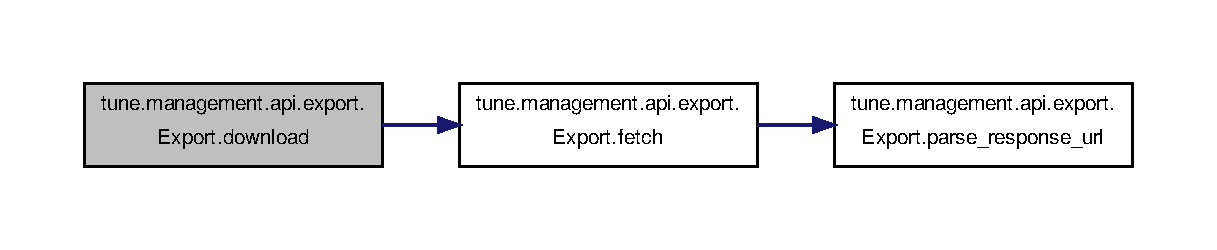
\includegraphics[width=350pt]{classtune_1_1management_1_1api_1_1export_1_1Export_a7c8f4a974ae5d915feb57bc4c3502f93_cgraph}
\end{center}
\end{figure}


\hypertarget{classtune_1_1management_1_1api_1_1export_1_1Export_af0819d2ba55d77f4f7f45ef5a91e1b96}{\index{tune\-::management\-::api\-::export\-::\-Export@{tune\-::management\-::api\-::export\-::\-Export}!fetch@{fetch}}
\index{fetch@{fetch}!tune::management::api::export::Export@{tune\-::management\-::api\-::export\-::\-Export}}
\subsubsection[{fetch}]{\setlength{\rightskip}{0pt plus 5cm}def tune.\-management.\-api.\-export.\-Export.\-fetch (
\begin{DoxyParamCaption}
\item[{}]{self, }
\item[{}]{job\-\_\-id, }
\item[{}]{report\-\_\-format, }
\item[{}]{verbose = {\ttfamily False}, }
\item[{}]{sleep = {\ttfamily 60}}
\end{DoxyParamCaption}
)}}\label{classtune_1_1management_1_1api_1_1export_1_1Export_af0819d2ba55d77f4f7f45ef5a91e1b96}


Definition at line 104 of file export.\-py.


\begin{DoxyCode}
104 
105     ):
106         \textcolor{keywordflow}{if} \textcolor{keywordflow}{not} self.\hyperlink{classtune_1_1management_1_1api_1_1export_1_1Export_ad9a517a5da2e72b2c26695151909ffe2}{\_\_api\_key} \textcolor{keywordflow}{or} len(self.\hyperlink{classtune_1_1management_1_1api_1_1export_1_1Export_ad9a517a5da2e72b2c26695151909ffe2}{\_\_api\_key}) < 1:
107             \textcolor{keywordflow}{raise} ValueError(\textcolor{stringliteral}{"Parameter 'api\_key' is not defined."})
108         \textcolor{keywordflow}{if} \textcolor{keywordflow}{not} job\_id \textcolor{keywordflow}{or} len(job\_id) < 1:
109             \textcolor{keywordflow}{raise} ValueError(\textcolor{stringliteral}{"Parameter 'job\_id' is not defined."})
110 
111         \textcolor{keywordflow}{return} ReportsBase.fetch(
112             self,
113             \textcolor{stringliteral}{"tune.management.api.export"},
114             \textcolor{stringliteral}{"Export"},
115             \textcolor{stringliteral}{"download"},
116             job\_id,
117             report\_format,
118             verbose,
119             sleep
120         )

\end{DoxyCode}


Here is the call graph for this function\-:
\nopagebreak
\begin{figure}[H]
\begin{center}
\leavevmode
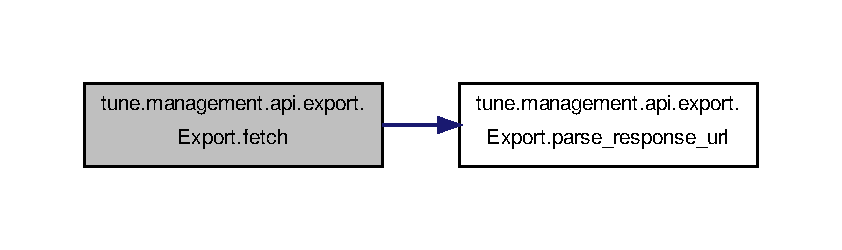
\includegraphics[width=350pt]{classtune_1_1management_1_1api_1_1export_1_1Export_af0819d2ba55d77f4f7f45ef5a91e1b96_cgraph}
\end{center}
\end{figure}




Here is the caller graph for this function\-:
\nopagebreak
\begin{figure}[H]
\begin{center}
\leavevmode
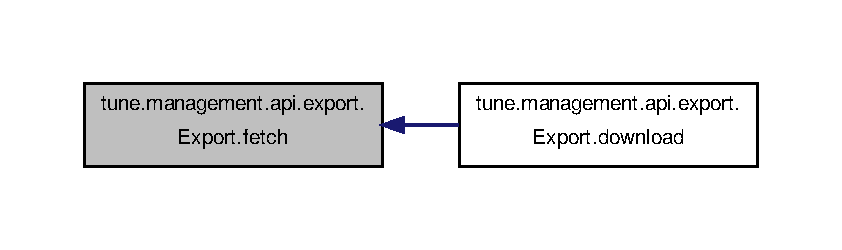
\includegraphics[width=350pt]{classtune_1_1management_1_1api_1_1export_1_1Export_af0819d2ba55d77f4f7f45ef5a91e1b96_icgraph}
\end{center}
\end{figure}


\hypertarget{classtune_1_1management_1_1api_1_1export_1_1Export_a39968f1bdbfdba59678de14db78c7ccc}{\index{tune\-::management\-::api\-::export\-::\-Export@{tune\-::management\-::api\-::export\-::\-Export}!parse\-\_\-response\-\_\-url@{parse\-\_\-response\-\_\-url}}
\index{parse\-\_\-response\-\_\-url@{parse\-\_\-response\-\_\-url}!tune::management::api::export::Export@{tune\-::management\-::api\-::export\-::\-Export}}
\subsubsection[{parse\-\_\-response\-\_\-url}]{\setlength{\rightskip}{0pt plus 5cm}def tune.\-management.\-api.\-export.\-Export.\-parse\-\_\-response\-\_\-url (
\begin{DoxyParamCaption}
\item[{}]{response}
\end{DoxyParamCaption}
)\hspace{0.3cm}{\ttfamily [static]}}}\label{classtune_1_1management_1_1api_1_1export_1_1Export_a39968f1bdbfdba59678de14db78c7ccc}


Helper function for parsing export status response to gather report url. 


\begin{DoxyParams}{Parameters}
{\em @see} & Response \\
\hline
\end{DoxyParams}
\begin{DoxyReturn}{Returns}
str Report Url 
\end{DoxyReturn}


Definition at line 127 of file export.\-py.


\begin{DoxyCode}
127 
128     ):
129         print(\textcolor{stringliteral}{"parse\_response\_url: \{\}"}.format(response))
130 
131         \textcolor{keywordflow}{if} \textcolor{keywordflow}{not} response:
132             \textcolor{keywordflow}{raise} ValueError(\textcolor{stringliteral}{"Parameter 'response' is not defined."})
133         \textcolor{keywordflow}{if} \textcolor{keywordflow}{not} response.data:
134             \textcolor{keywordflow}{raise} ValueError(\textcolor{stringliteral}{"Parameter 'response.data' is not defined."})
135         \textcolor{keywordflow}{if} \textcolor{stringliteral}{"data"} \textcolor{keywordflow}{not} \textcolor{keywordflow}{in} response.data:
136             \textcolor{keywordflow}{raise} ValueError(\textcolor{stringliteral}{"Parameter 'response.data['data'] is not defined."})
137         \textcolor{keywordflow}{if} \textcolor{stringliteral}{"url"} \textcolor{keywordflow}{not} \textcolor{keywordflow}{in} response.data[\textcolor{stringliteral}{"data"}]:
138             \textcolor{keywordflow}{raise} ValueError(\textcolor{stringliteral}{"Parameter 'response.data['data']['url'] is not defined."})
139 
140         url = response.data[\textcolor{stringliteral}{"data"}][\textcolor{stringliteral}{"url"}]
141 
142         \textcolor{keywordflow}{return} url
\end{DoxyCode}


Here is the caller graph for this function\-:
\nopagebreak
\begin{figure}[H]
\begin{center}
\leavevmode
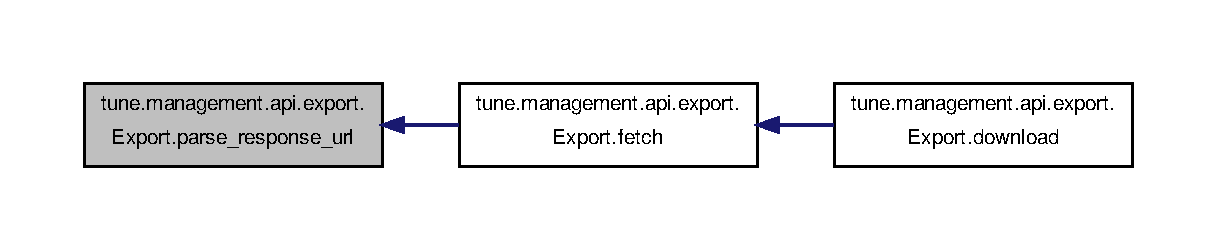
\includegraphics[width=350pt]{classtune_1_1management_1_1api_1_1export_1_1Export_a39968f1bdbfdba59678de14db78c7ccc_icgraph}
\end{center}
\end{figure}




\subsection{Member Data Documentation}
\hypertarget{classtune_1_1management_1_1api_1_1export_1_1Export_ad9a517a5da2e72b2c26695151909ffe2}{\index{tune\-::management\-::api\-::export\-::\-Export@{tune\-::management\-::api\-::export\-::\-Export}!\-\_\-\-\_\-api\-\_\-key@{\-\_\-\-\_\-api\-\_\-key}}
\index{\-\_\-\-\_\-api\-\_\-key@{\-\_\-\-\_\-api\-\_\-key}!tune::management::api::export::Export@{tune\-::management\-::api\-::export\-::\-Export}}
\subsubsection[{\-\_\-\-\_\-api\-\_\-key}]{\setlength{\rightskip}{0pt plus 5cm}tune.\-management.\-api.\-export.\-Export.\-\_\-\-\_\-api\-\_\-key\hspace{0.3cm}{\ttfamily [private]}}}\label{classtune_1_1management_1_1api_1_1export_1_1Export_ad9a517a5da2e72b2c26695151909ffe2}


Definition at line 57 of file export.\-py.



The documentation for this class was generated from the following file\-:\begin{DoxyCompactItemize}
\item 
tune/management/api/\hyperlink{export_8py}{export.\-py}\end{DoxyCompactItemize}

\hypertarget{classtune_1_1management_1_1api_1_1advertiser_1_1stats_1_1installs_1_1Installs}{\section{tune.\-management.\-api.\-advertiser.\-stats.\-installs.\-Installs Class Reference}
\label{classtune_1_1management_1_1api_1_1advertiser_1_1stats_1_1installs_1_1Installs}\index{tune.\-management.\-api.\-advertiser.\-stats.\-installs.\-Installs@{tune.\-management.\-api.\-advertiser.\-stats.\-installs.\-Installs}}
}


Inheritance diagram for tune.\-management.\-api.\-advertiser.\-stats.\-installs.\-Installs\-:
\nopagebreak
\begin{figure}[H]
\begin{center}
\leavevmode
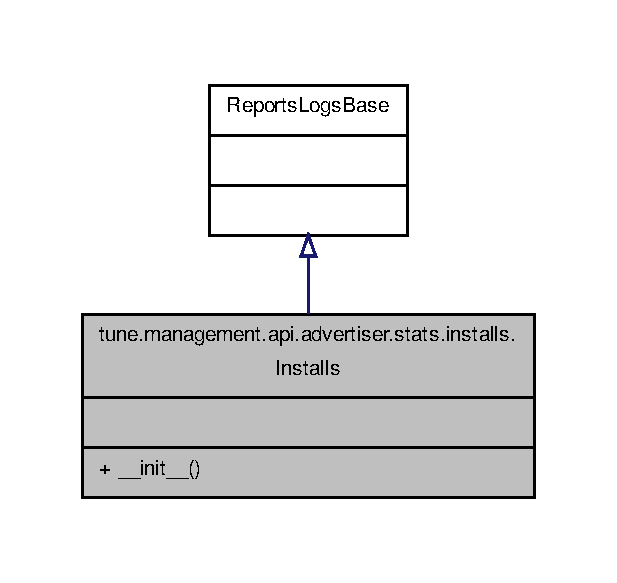
\includegraphics[width=296pt]{classtune_1_1management_1_1api_1_1advertiser_1_1stats_1_1installs_1_1Installs__inherit__graph}
\end{center}
\end{figure}


Collaboration diagram for tune.\-management.\-api.\-advertiser.\-stats.\-installs.\-Installs\-:
\nopagebreak
\begin{figure}[H]
\begin{center}
\leavevmode
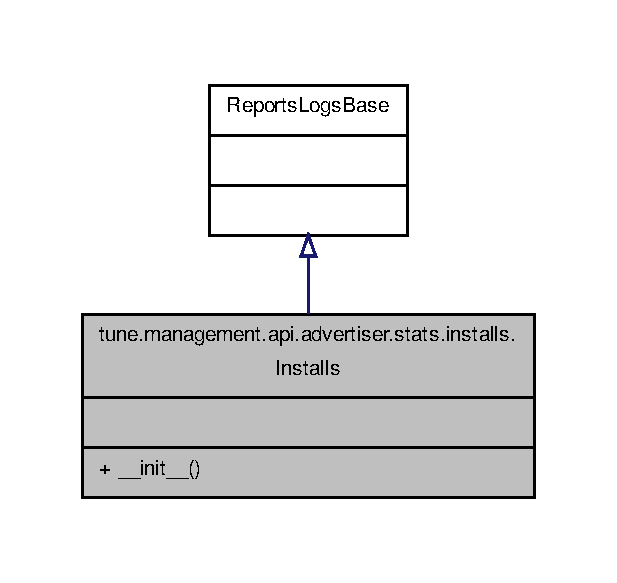
\includegraphics[width=296pt]{classtune_1_1management_1_1api_1_1advertiser_1_1stats_1_1installs_1_1Installs__coll__graph}
\end{center}
\end{figure}
\subsection*{Public Member Functions}
\begin{DoxyCompactItemize}
\item 
def \hyperlink{classtune_1_1management_1_1api_1_1advertiser_1_1stats_1_1installs_1_1Installs_a7d50d6bd87ad812e00353417a8fc2ea0}{\-\_\-\-\_\-init\-\_\-\-\_\-}
\begin{DoxyCompactList}\small\item\em The constructor. \end{DoxyCompactList}\end{DoxyCompactItemize}


\subsection{Detailed Description}


Definition at line 51 of file installs.\-py.



\subsection{Constructor \& Destructor Documentation}
\hypertarget{classtune_1_1management_1_1api_1_1advertiser_1_1stats_1_1installs_1_1Installs_a7d50d6bd87ad812e00353417a8fc2ea0}{\index{tune\-::management\-::api\-::advertiser\-::stats\-::installs\-::\-Installs@{tune\-::management\-::api\-::advertiser\-::stats\-::installs\-::\-Installs}!\-\_\-\-\_\-init\-\_\-\-\_\-@{\-\_\-\-\_\-init\-\_\-\-\_\-}}
\index{\-\_\-\-\_\-init\-\_\-\-\_\-@{\-\_\-\-\_\-init\-\_\-\-\_\-}!tune::management::api::advertiser::stats::installs::Installs@{tune\-::management\-::api\-::advertiser\-::stats\-::installs\-::\-Installs}}
\subsubsection[{\-\_\-\-\_\-init\-\_\-\-\_\-}]{\setlength{\rightskip}{0pt plus 5cm}def tune.\-management.\-api.\-advertiser.\-stats.\-installs.\-Installs.\-\_\-\-\_\-init\-\_\-\-\_\- (
\begin{DoxyParamCaption}
\item[{}]{self, }
\item[{}]{api\-\_\-key, }
\item[{}]{validate = {\ttfamily False}}
\end{DoxyParamCaption}
)}}\label{classtune_1_1management_1_1api_1_1advertiser_1_1stats_1_1installs_1_1Installs_a7d50d6bd87ad812e00353417a8fc2ea0}


The constructor. 


\begin{DoxyParams}{Parameters}
{\em str} & api\-\_\-key Mobile\-App\-Tracking A\-P\-I Key. \\
\hline
{\em bool} & validate Validate fields used by actions. \\
\hline
\end{DoxyParams}


Definition at line 62 of file installs.\-py.


\begin{DoxyCode}
62 
63         ):
64         ReportsLogsBase.\_\_init\_\_(
65             self,
66             \textcolor{stringliteral}{"advertiser/stats/installs"},
67             api\_key,
68             \textcolor{keyword}{True},
69             \textcolor{keyword}{True},
70             validate
71         )
\end{DoxyCode}


The documentation for this class was generated from the following file\-:\begin{DoxyCompactItemize}
\item 
tune/management/api/advertiser/stats/\hyperlink{installs_8py}{installs.\-py}\end{DoxyCompactItemize}

\hypertarget{classtune_1_1management_1_1api_1_1advertiser_1_1stats_1_1ltv_1_1LTV}{\section{tune.\-management.\-api.\-advertiser.\-stats.\-ltv.\-L\-T\-V Class Reference}
\label{classtune_1_1management_1_1api_1_1advertiser_1_1stats_1_1ltv_1_1LTV}\index{tune.\-management.\-api.\-advertiser.\-stats.\-ltv.\-L\-T\-V@{tune.\-management.\-api.\-advertiser.\-stats.\-ltv.\-L\-T\-V}}
}


Inheritance diagram for tune.\-management.\-api.\-advertiser.\-stats.\-ltv.\-L\-T\-V\-:
\nopagebreak
\begin{figure}[H]
\begin{center}
\leavevmode
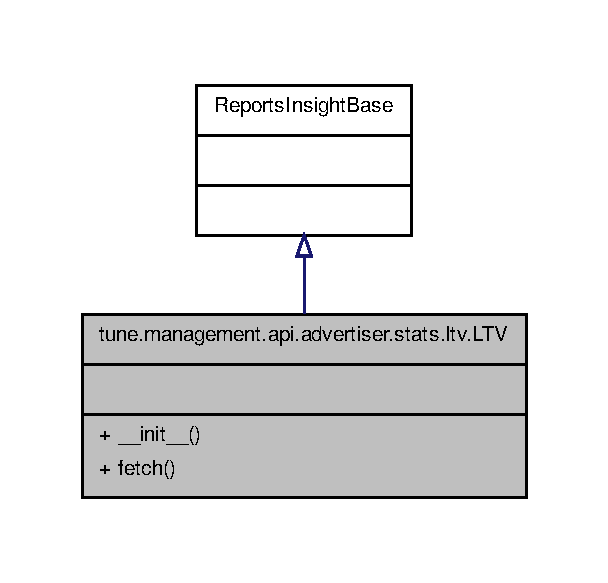
\includegraphics[width=292pt]{classtune_1_1management_1_1api_1_1advertiser_1_1stats_1_1ltv_1_1LTV__inherit__graph}
\end{center}
\end{figure}


Collaboration diagram for tune.\-management.\-api.\-advertiser.\-stats.\-ltv.\-L\-T\-V\-:
\nopagebreak
\begin{figure}[H]
\begin{center}
\leavevmode
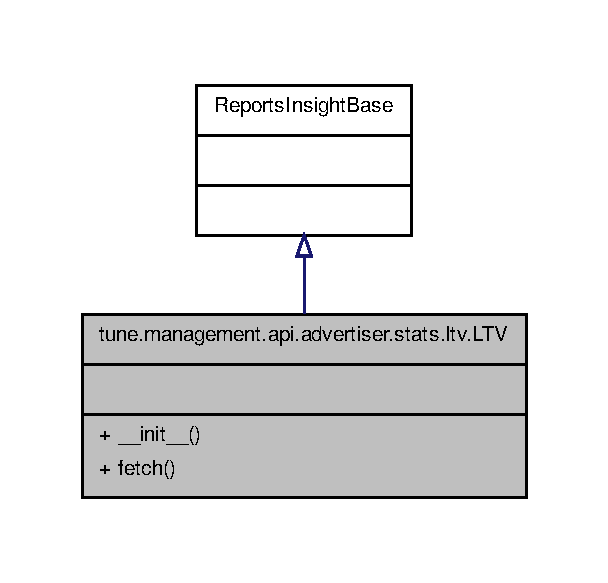
\includegraphics[width=292pt]{classtune_1_1management_1_1api_1_1advertiser_1_1stats_1_1ltv_1_1LTV__coll__graph}
\end{center}
\end{figure}
\subsection*{Public Member Functions}
\begin{DoxyCompactItemize}
\item 
def \hyperlink{classtune_1_1management_1_1api_1_1advertiser_1_1stats_1_1ltv_1_1LTV_af779610e2442bd593981f26fe1da0563}{\-\_\-\-\_\-init\-\_\-\-\_\-}
\begin{DoxyCompactList}\small\item\em The constructor. \end{DoxyCompactList}\item 
def \hyperlink{classtune_1_1management_1_1api_1_1advertiser_1_1stats_1_1ltv_1_1LTV_a10f3a6a49f64a203162ae337ff5ccefd}{fetch}
\begin{DoxyCompactList}\small\item\em Helper function for fetching report document given provided job identifier. \end{DoxyCompactList}\end{DoxyCompactItemize}


\subsection{Detailed Description}


Definition at line 51 of file ltv.\-py.



\subsection{Constructor \& Destructor Documentation}
\hypertarget{classtune_1_1management_1_1api_1_1advertiser_1_1stats_1_1ltv_1_1LTV_af779610e2442bd593981f26fe1da0563}{\index{tune\-::management\-::api\-::advertiser\-::stats\-::ltv\-::\-L\-T\-V@{tune\-::management\-::api\-::advertiser\-::stats\-::ltv\-::\-L\-T\-V}!\-\_\-\-\_\-init\-\_\-\-\_\-@{\-\_\-\-\_\-init\-\_\-\-\_\-}}
\index{\-\_\-\-\_\-init\-\_\-\-\_\-@{\-\_\-\-\_\-init\-\_\-\-\_\-}!tune::management::api::advertiser::stats::ltv::LTV@{tune\-::management\-::api\-::advertiser\-::stats\-::ltv\-::\-L\-T\-V}}
\subsubsection[{\-\_\-\-\_\-init\-\_\-\-\_\-}]{\setlength{\rightskip}{0pt plus 5cm}def tune.\-management.\-api.\-advertiser.\-stats.\-ltv.\-L\-T\-V.\-\_\-\-\_\-init\-\_\-\-\_\- (
\begin{DoxyParamCaption}
\item[{}]{self, }
\item[{}]{api\-\_\-key, }
\item[{}]{validate = {\ttfamily False}}
\end{DoxyParamCaption}
)}}\label{classtune_1_1management_1_1api_1_1advertiser_1_1stats_1_1ltv_1_1LTV_af779610e2442bd593981f26fe1da0563}


The constructor. 


\begin{DoxyParams}{Parameters}
{\em str} & api\-\_\-key Mobile\-App\-Tracking A\-P\-I Key. \\
\hline
{\em bool} & validate Validate fields used by actions. \\
\hline
\end{DoxyParams}


Definition at line 62 of file ltv.\-py.


\begin{DoxyCode}
62 
63         ):
64         ReportsInsightBase.\_\_init\_\_(
65             self,
66             \textcolor{stringliteral}{"advertiser/stats/ltv"},
67             api\_key,
68             \textcolor{keyword}{False},
69             \textcolor{keyword}{True},
70             validate
71         )

\end{DoxyCode}


Here is the call graph for this function\-:
\nopagebreak
\begin{figure}[H]
\begin{center}
\leavevmode
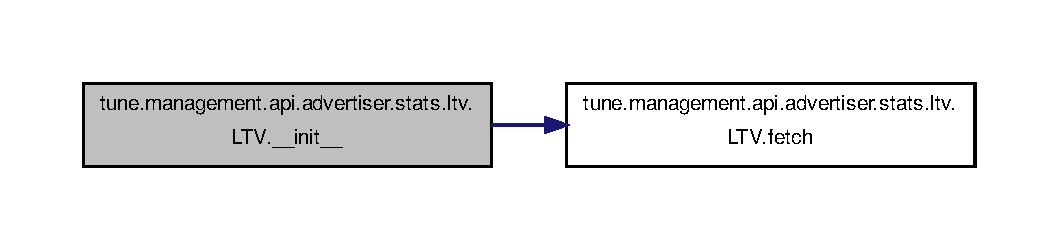
\includegraphics[width=350pt]{classtune_1_1management_1_1api_1_1advertiser_1_1stats_1_1ltv_1_1LTV_af779610e2442bd593981f26fe1da0563_cgraph}
\end{center}
\end{figure}




\subsection{Member Function Documentation}
\hypertarget{classtune_1_1management_1_1api_1_1advertiser_1_1stats_1_1ltv_1_1LTV_a10f3a6a49f64a203162ae337ff5ccefd}{\index{tune\-::management\-::api\-::advertiser\-::stats\-::ltv\-::\-L\-T\-V@{tune\-::management\-::api\-::advertiser\-::stats\-::ltv\-::\-L\-T\-V}!fetch@{fetch}}
\index{fetch@{fetch}!tune::management::api::advertiser::stats::ltv::LTV@{tune\-::management\-::api\-::advertiser\-::stats\-::ltv\-::\-L\-T\-V}}
\subsubsection[{fetch}]{\setlength{\rightskip}{0pt plus 5cm}def tune.\-management.\-api.\-advertiser.\-stats.\-ltv.\-L\-T\-V.\-fetch (
\begin{DoxyParamCaption}
\item[{}]{self, }
\item[{}]{job\-\_\-id, }
\item[{}]{report\-\_\-format = {\ttfamily \char`\"{}csv\char`\"{}}, }
\item[{}]{verbose = {\ttfamily False}, }
\item[{}]{sleep = {\ttfamily 60~\#~seconds~~~~~~~~~~~~~\#}}
\end{DoxyParamCaption}
)}}\label{classtune_1_1management_1_1api_1_1advertiser_1_1stats_1_1ltv_1_1LTV_a10f3a6a49f64a203162ae337ff5ccefd}


Helper function for fetching report document given provided job identifier. 


\begin{DoxyParams}{Parameters}
{\em string} & job\-\_\-id Job Identifier of report on queue. \\
\hline
{\em string} & report\-\_\-format Requested document format\-: csv, json \\
\hline
{\em bool} & verbose For debugging purposes only. \\
\hline
{\em int} & sleep How long thread should sleep before next status request.\\
\hline
\end{DoxyParams}
\begin{DoxyReturn}{Returns}
object 
\end{DoxyReturn}


Definition at line 87 of file ltv.\-py.


\begin{DoxyCode}
87 
88     ):
89         \textcolor{keywordflow}{return} ReportsInsightBase.fetch(
90             self,
91             \textcolor{stringliteral}{"tune.management.api.advertiser.stats.ltv"},
92             self.\_\_class\_\_.\_\_name\_\_,
93             job\_id,
94             report\_format,
95             verbose,
96             sleep \textcolor{comment}{# seconds}
97         )
\end{DoxyCode}


Here is the caller graph for this function\-:
\nopagebreak
\begin{figure}[H]
\begin{center}
\leavevmode
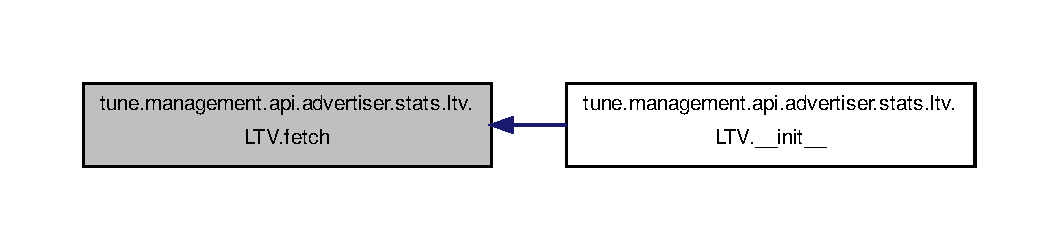
\includegraphics[width=350pt]{classtune_1_1management_1_1api_1_1advertiser_1_1stats_1_1ltv_1_1LTV_a10f3a6a49f64a203162ae337ff5ccefd_icgraph}
\end{center}
\end{figure}




The documentation for this class was generated from the following file\-:\begin{DoxyCompactItemize}
\item 
tune/management/api/advertiser/stats/\hyperlink{ltv_8py}{ltv.\-py}\end{DoxyCompactItemize}

\hypertarget{classobject}{\section{object Class Reference}
\label{classobject}\index{object@{object}}
}


Inheritance diagram for object\-:
\nopagebreak
\begin{figure}[H]
\begin{center}
\leavevmode
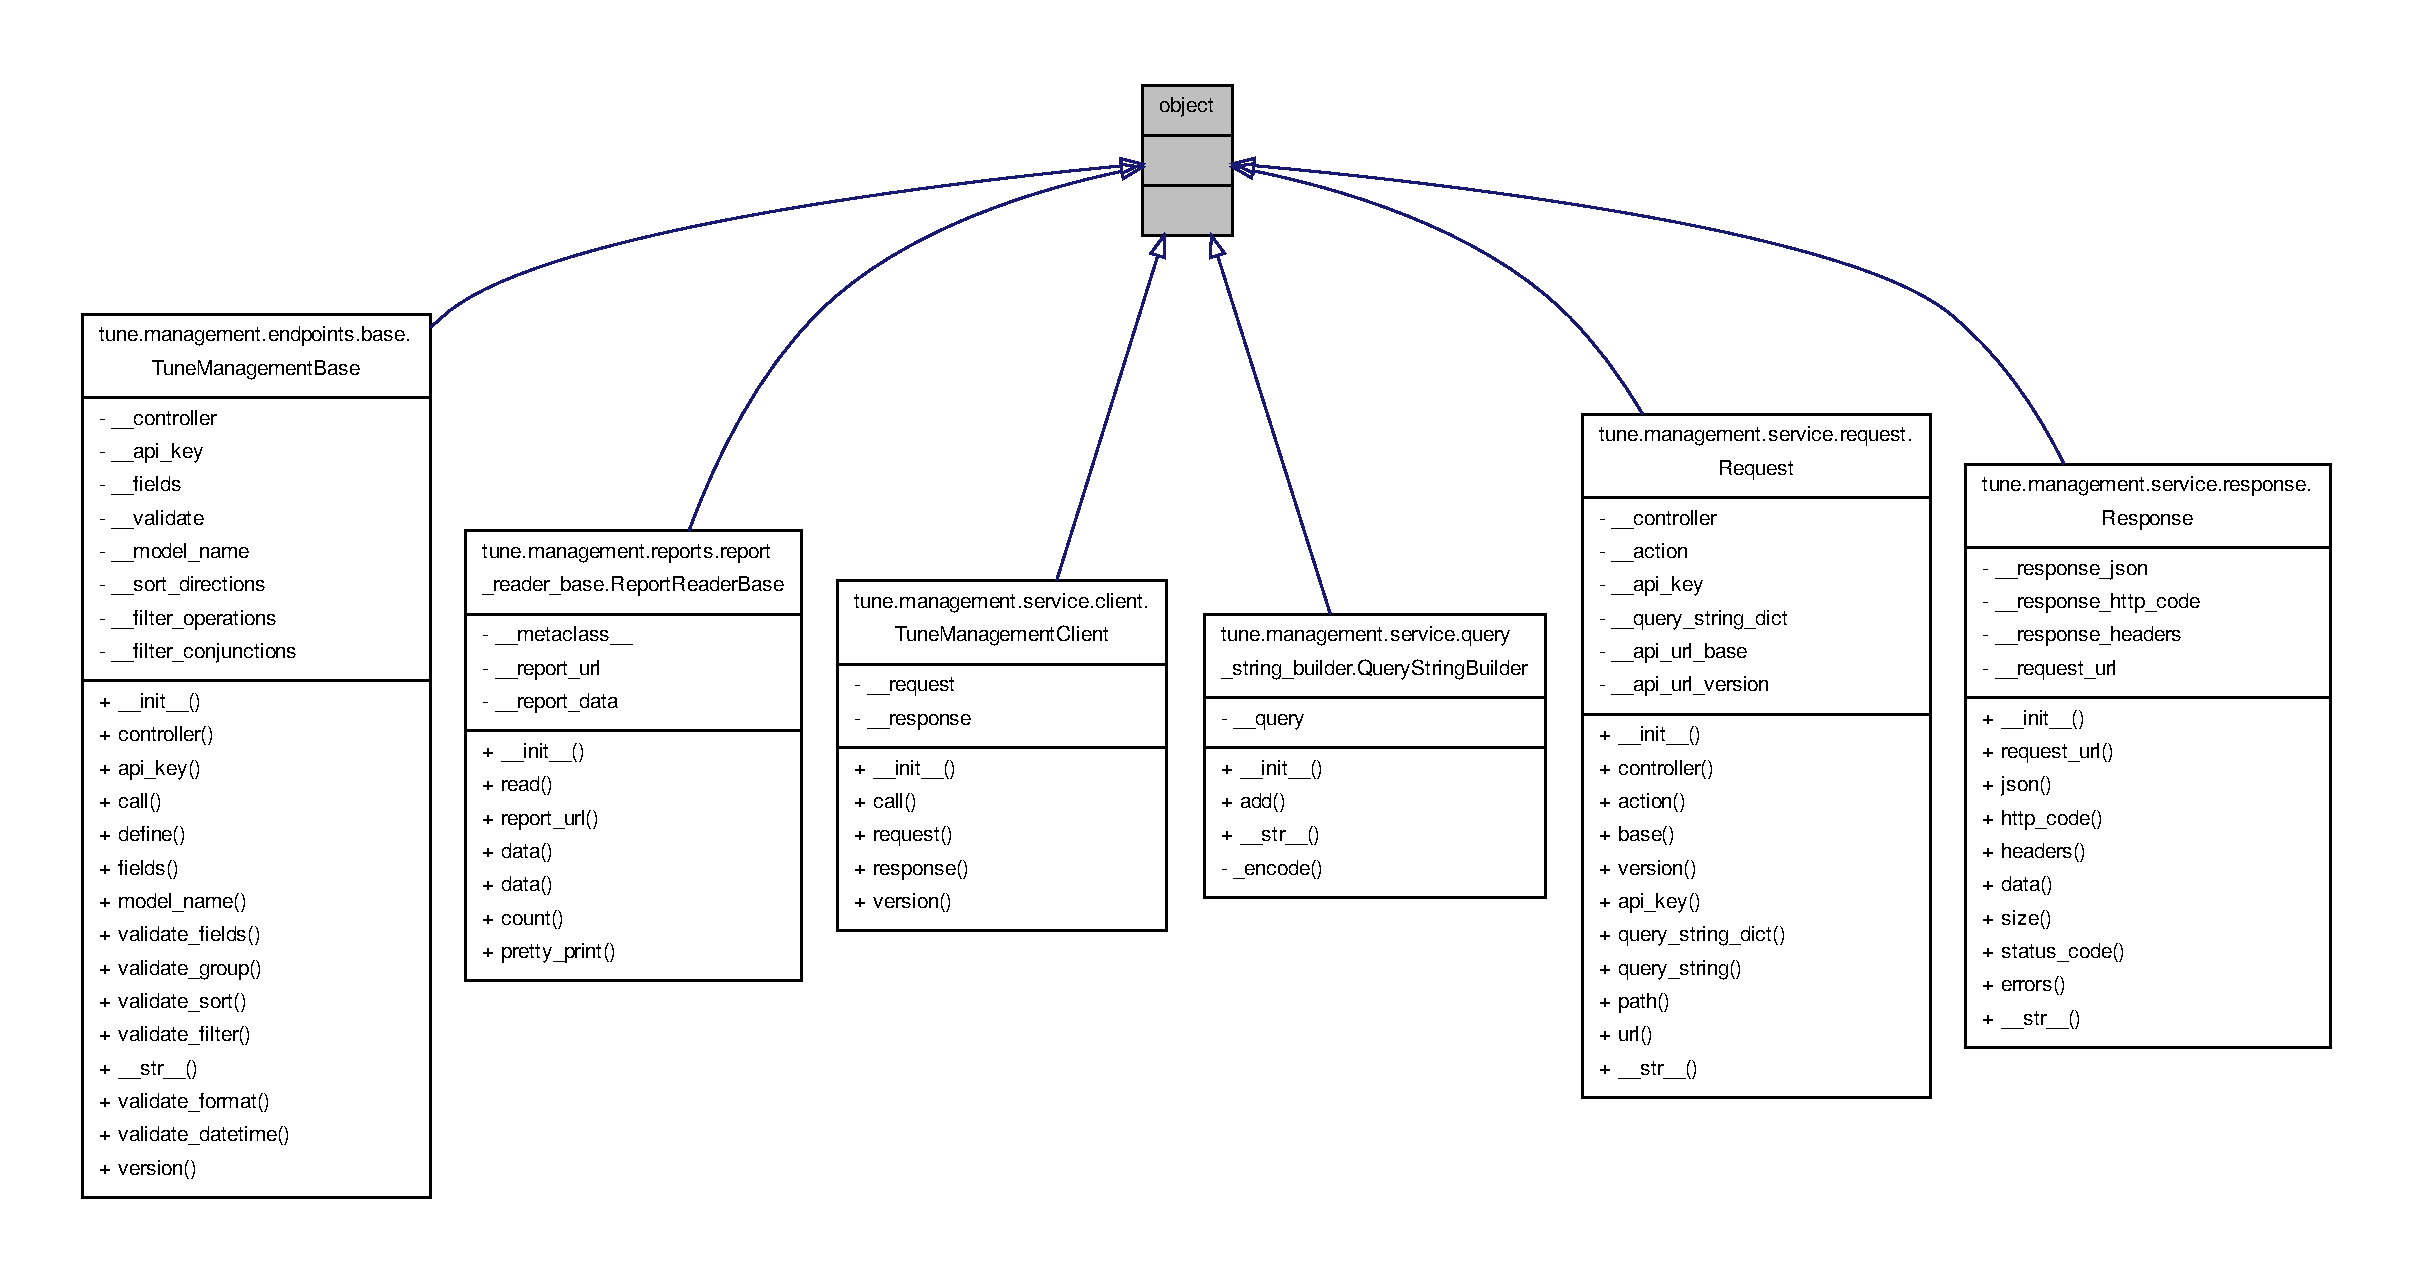
\includegraphics[width=350pt]{classobject__inherit__graph}
\end{center}
\end{figure}


Collaboration diagram for object\-:
\nopagebreak
\begin{figure}[H]
\begin{center}
\leavevmode
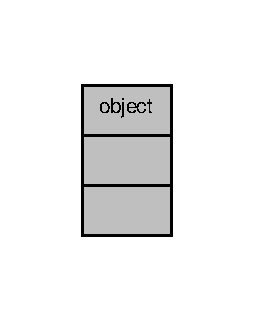
\includegraphics[width=122pt]{classobject__coll__graph}
\end{center}
\end{figure}


The documentation for this class was generated from the following file\-:\begin{DoxyCompactItemize}
\item 
tune/management/service/\hyperlink{query__string__builder_8py}{query\-\_\-string\-\_\-builder.\-py}\end{DoxyCompactItemize}

\hypertarget{classtune_1_1management_1_1api_1_1advertiser_1_1stats_1_1postbacks_1_1Postbacks}{\section{tune.\-management.\-api.\-advertiser.\-stats.\-postbacks.\-Postbacks Class Reference}
\label{classtune_1_1management_1_1api_1_1advertiser_1_1stats_1_1postbacks_1_1Postbacks}\index{tune.\-management.\-api.\-advertiser.\-stats.\-postbacks.\-Postbacks@{tune.\-management.\-api.\-advertiser.\-stats.\-postbacks.\-Postbacks}}
}


Inheritance diagram for tune.\-management.\-api.\-advertiser.\-stats.\-postbacks.\-Postbacks\-:
\nopagebreak
\begin{figure}[H]
\begin{center}
\leavevmode
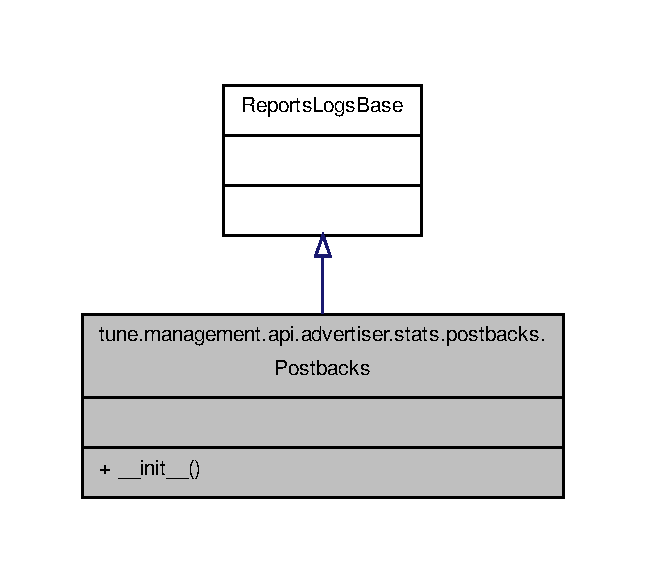
\includegraphics[width=310pt]{classtune_1_1management_1_1api_1_1advertiser_1_1stats_1_1postbacks_1_1Postbacks__inherit__graph}
\end{center}
\end{figure}


Collaboration diagram for tune.\-management.\-api.\-advertiser.\-stats.\-postbacks.\-Postbacks\-:
\nopagebreak
\begin{figure}[H]
\begin{center}
\leavevmode
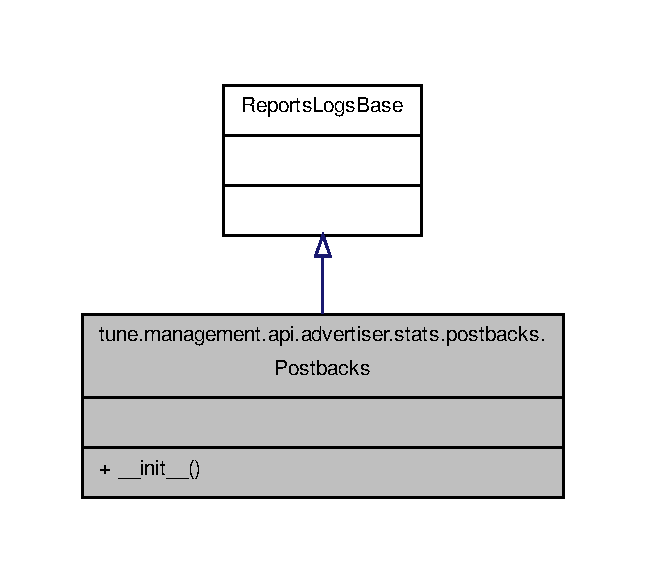
\includegraphics[width=310pt]{classtune_1_1management_1_1api_1_1advertiser_1_1stats_1_1postbacks_1_1Postbacks__coll__graph}
\end{center}
\end{figure}
\subsection*{Public Member Functions}
\begin{DoxyCompactItemize}
\item 
def \hyperlink{classtune_1_1management_1_1api_1_1advertiser_1_1stats_1_1postbacks_1_1Postbacks_a4c0dc04eacce08fdf61e8a9812892645}{\-\_\-\-\_\-init\-\_\-\-\_\-}
\begin{DoxyCompactList}\small\item\em The constructor. \end{DoxyCompactList}\end{DoxyCompactItemize}


\subsection{Detailed Description}


Definition at line 51 of file postbacks.\-py.



\subsection{Constructor \& Destructor Documentation}
\hypertarget{classtune_1_1management_1_1api_1_1advertiser_1_1stats_1_1postbacks_1_1Postbacks_a4c0dc04eacce08fdf61e8a9812892645}{\index{tune\-::management\-::api\-::advertiser\-::stats\-::postbacks\-::\-Postbacks@{tune\-::management\-::api\-::advertiser\-::stats\-::postbacks\-::\-Postbacks}!\-\_\-\-\_\-init\-\_\-\-\_\-@{\-\_\-\-\_\-init\-\_\-\-\_\-}}
\index{\-\_\-\-\_\-init\-\_\-\-\_\-@{\-\_\-\-\_\-init\-\_\-\-\_\-}!tune::management::api::advertiser::stats::postbacks::Postbacks@{tune\-::management\-::api\-::advertiser\-::stats\-::postbacks\-::\-Postbacks}}
\subsubsection[{\-\_\-\-\_\-init\-\_\-\-\_\-}]{\setlength{\rightskip}{0pt plus 5cm}def tune.\-management.\-api.\-advertiser.\-stats.\-postbacks.\-Postbacks.\-\_\-\-\_\-init\-\_\-\-\_\- (
\begin{DoxyParamCaption}
\item[{}]{self, }
\item[{}]{api\-\_\-key, }
\item[{}]{validate = {\ttfamily False}}
\end{DoxyParamCaption}
)}}\label{classtune_1_1management_1_1api_1_1advertiser_1_1stats_1_1postbacks_1_1Postbacks_a4c0dc04eacce08fdf61e8a9812892645}


The constructor. 


\begin{DoxyParams}{Parameters}
{\em str} & api\-\_\-key Mobile\-App\-Tracking A\-P\-I Key. \\
\hline
{\em bool} & validate Validate fields used by actions. \\
\hline
\end{DoxyParams}


Definition at line 62 of file postbacks.\-py.


\begin{DoxyCode}
62 
63         ):
64         ReportsLogsBase.\_\_init\_\_(
65             self,
66             \textcolor{stringliteral}{"advertiser/stats/postbacks"},
67             api\_key,
68             \textcolor{keyword}{False},
69             \textcolor{keyword}{True},
70             validate
71         )
\end{DoxyCode}


The documentation for this class was generated from the following file\-:\begin{DoxyCompactItemize}
\item 
tune/management/api/advertiser/stats/\hyperlink{postbacks_8py}{postbacks.\-py}\end{DoxyCompactItemize}

\hypertarget{classtune_1_1management_1_1service_1_1proxy_1_1Proxy}{\section{tune.\-management.\-service.\-proxy.\-Proxy Class Reference}
\label{classtune_1_1management_1_1service_1_1proxy_1_1Proxy}\index{tune.\-management.\-service.\-proxy.\-Proxy@{tune.\-management.\-service.\-proxy.\-Proxy}}
}


Service proxy class for connecting to Tune Management A\-P\-I service.  




Collaboration diagram for tune.\-management.\-service.\-proxy.\-Proxy\-:
\nopagebreak
\begin{figure}[H]
\begin{center}
\leavevmode
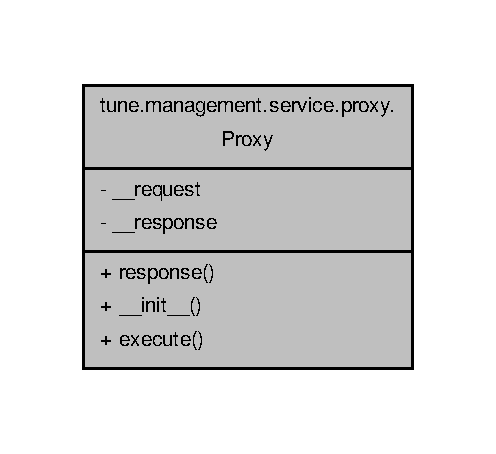
\includegraphics[width=238pt]{classtune_1_1management_1_1service_1_1proxy_1_1Proxy__coll__graph}
\end{center}
\end{figure}
\subsection*{Public Member Functions}
\begin{DoxyCompactItemize}
\item 
def \hyperlink{classtune_1_1management_1_1service_1_1proxy_1_1Proxy_a0b3f63ff9936b0857c4ae47b38b5f926}{response}
\begin{DoxyCompactList}\small\item\em Full response object to Tune Management A\-P\-I service. \end{DoxyCompactList}\item 
def \hyperlink{classtune_1_1management_1_1service_1_1proxy_1_1Proxy_a8fe235be39f55c27191277d95d7ef25f}{\-\_\-\-\_\-init\-\_\-\-\_\-}
\item 
def \hyperlink{classtune_1_1management_1_1service_1_1proxy_1_1Proxy_af3c0cf7d72b8b929b0e5fbbd1611c7ef}{execute}
\begin{DoxyCompactList}\small\item\em H\-T\-T\-P P\-O\-S\-T request to Tune Mobile\-App\-Tracking Management A\-P\-I. \end{DoxyCompactList}\end{DoxyCompactItemize}
\subsection*{Static Private Attributes}
\begin{DoxyCompactItemize}
\item 
\hyperlink{classtune_1_1management_1_1service_1_1proxy_1_1Proxy_a8152a63a83044f4106c6202e1d3621a8}{\-\_\-\-\_\-request} = None
\item 
\hyperlink{classtune_1_1management_1_1service_1_1proxy_1_1Proxy_a1f7385defeef51c4ec8ca120c720dcfd}{\-\_\-\-\_\-response} = None
\end{DoxyCompactItemize}


\subsection{Detailed Description}
Service proxy class for connecting to Tune Management A\-P\-I service. 

Attributes\-: \-\_\-\-\_\-request\-: Tune Management A\-P\-I request object\par
 \-\_\-\-\_\-response\-: Tune Management A\-P\-I response object\par


Definition at line 65 of file proxy.\-py.



\subsection{Constructor \& Destructor Documentation}
\hypertarget{classtune_1_1management_1_1service_1_1proxy_1_1Proxy_a8fe235be39f55c27191277d95d7ef25f}{\index{tune\-::management\-::service\-::proxy\-::\-Proxy@{tune\-::management\-::service\-::proxy\-::\-Proxy}!\-\_\-\-\_\-init\-\_\-\-\_\-@{\-\_\-\-\_\-init\-\_\-\-\_\-}}
\index{\-\_\-\-\_\-init\-\_\-\-\_\-@{\-\_\-\-\_\-init\-\_\-\-\_\-}!tune::management::service::proxy::Proxy@{tune\-::management\-::service\-::proxy\-::\-Proxy}}
\subsubsection[{\-\_\-\-\_\-init\-\_\-\-\_\-}]{\setlength{\rightskip}{0pt plus 5cm}def tune.\-management.\-service.\-proxy.\-Proxy.\-\_\-\-\_\-init\-\_\-\-\_\- (
\begin{DoxyParamCaption}
\item[{}]{self, }
\item[{}]{request}
\end{DoxyParamCaption}
)}}\label{classtune_1_1management_1_1service_1_1proxy_1_1Proxy_a8fe235be39f55c27191277d95d7ef25f}


Definition at line 76 of file proxy.\-py.


\begin{DoxyCode}
76 
77     \textcolor{keyword}{def }\hyperlink{classtune_1_1management_1_1service_1_1proxy_1_1Proxy_a8fe235be39f55c27191277d95d7ef25f}{\_\_init\_\_}(self, request):
78         \textcolor{keywordflow}{if} request \textcolor{keywordflow}{is} \textcolor{keywordtype}{None} \textcolor{keywordflow}{or} \textcolor{keywordflow}{not} isinstance(request, Request):
79             \textcolor{keywordflow}{raise} ValueError(\textcolor{stringliteral}{"Invalid request provided."})
80 
81         self.\hyperlink{classtune_1_1management_1_1service_1_1proxy_1_1Proxy_a8152a63a83044f4106c6202e1d3621a8}{\_\_request} = request

\end{DoxyCode}


\subsection{Member Function Documentation}
\hypertarget{classtune_1_1management_1_1service_1_1proxy_1_1Proxy_af3c0cf7d72b8b929b0e5fbbd1611c7ef}{\index{tune\-::management\-::service\-::proxy\-::\-Proxy@{tune\-::management\-::service\-::proxy\-::\-Proxy}!execute@{execute}}
\index{execute@{execute}!tune::management::service::proxy::Proxy@{tune\-::management\-::service\-::proxy\-::\-Proxy}}
\subsubsection[{execute}]{\setlength{\rightskip}{0pt plus 5cm}def tune.\-management.\-service.\-proxy.\-Proxy.\-execute (
\begin{DoxyParamCaption}
\item[{}]{self}
\end{DoxyParamCaption}
)}}\label{classtune_1_1management_1_1service_1_1proxy_1_1Proxy_af3c0cf7d72b8b929b0e5fbbd1611c7ef}


H\-T\-T\-P P\-O\-S\-T request to Tune Mobile\-App\-Tracking Management A\-P\-I. 

Returns\-: bool\-: True upon success. 

Definition at line 88 of file proxy.\-py.


\begin{DoxyCode}
88 
89     \textcolor{keyword}{def }\hyperlink{classtune_1_1management_1_1service_1_1proxy_1_1Proxy_af3c0cf7d72b8b929b0e5fbbd1611c7ef}{execute}(self):
90         \textcolor{keywordflow}{if} self.\hyperlink{classtune_1_1management_1_1service_1_1proxy_1_1Proxy_a8152a63a83044f4106c6202e1d3621a8}{\_\_request} \textcolor{keywordflow}{is} \textcolor{keywordtype}{None}:
91             \textcolor{keywordflow}{raise} TuneSdkException(\textcolor{stringliteral}{'Request is not set.'})
92 
93         \textcolor{keywordflow}{try}:
94             request\_url = self.\_\_request.url
95             self.\hyperlink{classtune_1_1management_1_1service_1_1proxy_1_1Proxy_a1f7385defeef51c4ec8ca120c720dcfd}{\_\_response} = urllib.request.urlopen(request\_url)
96 
97         \textcolor{keywordflow}{except} TuneSdkException \textcolor{keyword}{as} ex:
98             \textcolor{keywordflow}{raise}
99         \textcolor{keywordflow}{except} TuneServiceException \textcolor{keyword}{as} ex:
100             \textcolor{keywordflow}{raise}
101         \textcolor{keywordflow}{except} urllib.error.URLError \textcolor{keyword}{as} ex:
102             \textcolor{keywordflow}{raise} TuneServiceException(\textcolor{stringliteral}{"URLError: \{\}"}.format(str(ex)))
103         \textcolor{keywordflow}{except} urllib.error.HTTPError \textcolor{keyword}{as} ex:
104             \textcolor{keywordflow}{raise} TuneServiceException(\textcolor{stringliteral}{"HTTPError: \{\}"}.format(str(ex)))
105         \textcolor{keywordflow}{except} Exception \textcolor{keyword}{as} ex:
106             \textcolor{keywordflow}{raise} TuneSdkException(
107                 \textcolor{stringliteral}{"Failed to post request: (Error:\{0\}, Url:\{1\})"}.format(
108                     str(ex),
109                     self.\_\_request.url),
110                 ex
111             )
112 
113         \textcolor{keywordflow}{return} \textcolor{keyword}{True}
\end{DoxyCode}
\hypertarget{classtune_1_1management_1_1service_1_1proxy_1_1Proxy_a0b3f63ff9936b0857c4ae47b38b5f926}{\index{tune\-::management\-::service\-::proxy\-::\-Proxy@{tune\-::management\-::service\-::proxy\-::\-Proxy}!response@{response}}
\index{response@{response}!tune::management::service::proxy::Proxy@{tune\-::management\-::service\-::proxy\-::\-Proxy}}
\subsubsection[{response}]{\setlength{\rightskip}{0pt plus 5cm}def tune.\-management.\-service.\-proxy.\-Proxy.\-response (
\begin{DoxyParamCaption}
\item[{}]{self}
\end{DoxyParamCaption}
)}}\label{classtune_1_1management_1_1service_1_1proxy_1_1Proxy_a0b3f63ff9936b0857c4ae47b38b5f926}


Full response object to Tune Management A\-P\-I service. 



Definition at line 73 of file proxy.\-py.


\begin{DoxyCode}
73 
74     \textcolor{keyword}{def }\hyperlink{classtune_1_1management_1_1service_1_1proxy_1_1Proxy_a0b3f63ff9936b0857c4ae47b38b5f926}{response}(self):
75         \textcolor{keywordflow}{return} self.\hyperlink{classtune_1_1management_1_1service_1_1proxy_1_1Proxy_a1f7385defeef51c4ec8ca120c720dcfd}{\_\_response}

\end{DoxyCode}


\subsection{Member Data Documentation}
\hypertarget{classtune_1_1management_1_1service_1_1proxy_1_1Proxy_a8152a63a83044f4106c6202e1d3621a8}{\index{tune\-::management\-::service\-::proxy\-::\-Proxy@{tune\-::management\-::service\-::proxy\-::\-Proxy}!\-\_\-\-\_\-request@{\-\_\-\-\_\-request}}
\index{\-\_\-\-\_\-request@{\-\_\-\-\_\-request}!tune::management::service::proxy::Proxy@{tune\-::management\-::service\-::proxy\-::\-Proxy}}
\subsubsection[{\-\_\-\-\_\-request}]{\setlength{\rightskip}{0pt plus 5cm}tune.\-management.\-service.\-proxy.\-Proxy.\-\_\-\-\_\-request = None\hspace{0.3cm}{\ttfamily [static]}, {\ttfamily [private]}}}\label{classtune_1_1management_1_1service_1_1proxy_1_1Proxy_a8152a63a83044f4106c6202e1d3621a8}


Definition at line 67 of file proxy.\-py.

\hypertarget{classtune_1_1management_1_1service_1_1proxy_1_1Proxy_a1f7385defeef51c4ec8ca120c720dcfd}{\index{tune\-::management\-::service\-::proxy\-::\-Proxy@{tune\-::management\-::service\-::proxy\-::\-Proxy}!\-\_\-\-\_\-response@{\-\_\-\-\_\-response}}
\index{\-\_\-\-\_\-response@{\-\_\-\-\_\-response}!tune::management::service::proxy::Proxy@{tune\-::management\-::service\-::proxy\-::\-Proxy}}
\subsubsection[{\-\_\-\-\_\-response}]{\setlength{\rightskip}{0pt plus 5cm}tune.\-management.\-service.\-proxy.\-Proxy.\-\_\-\-\_\-response = None\hspace{0.3cm}{\ttfamily [static]}, {\ttfamily [private]}}}\label{classtune_1_1management_1_1service_1_1proxy_1_1Proxy_a1f7385defeef51c4ec8ca120c720dcfd}


Definition at line 68 of file proxy.\-py.



The documentation for this class was generated from the following file\-:\begin{DoxyCompactItemize}
\item 
tune/management/service/\hyperlink{proxy_8py}{proxy.\-py}\end{DoxyCompactItemize}

\hypertarget{classtune_1_1management_1_1service_1_1query__string__builder_1_1QueryStringBuilder}{\section{tune.\-management.\-service.\-query\-\_\-string\-\_\-builder.\-Query\-String\-Builder Class Reference}
\label{classtune_1_1management_1_1service_1_1query__string__builder_1_1QueryStringBuilder}\index{tune.\-management.\-service.\-query\-\_\-string\-\_\-builder.\-Query\-String\-Builder@{tune.\-management.\-service.\-query\-\_\-string\-\_\-builder.\-Query\-String\-Builder}}
}


Build Query String provide with dictionary of query parameters.  




Inheritance diagram for tune.\-management.\-service.\-query\-\_\-string\-\_\-builder.\-Query\-String\-Builder\-:
\nopagebreak
\begin{figure}[H]
\begin{center}
\leavevmode
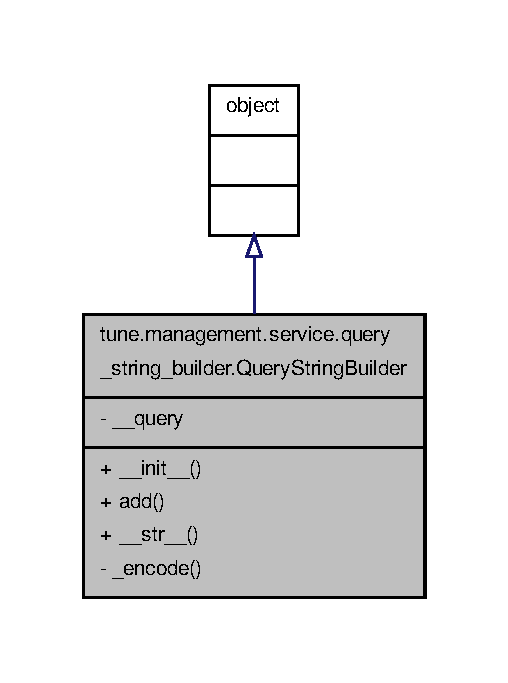
\includegraphics[width=244pt]{classtune_1_1management_1_1service_1_1query__string__builder_1_1QueryStringBuilder__inherit__graph}
\end{center}
\end{figure}


Collaboration diagram for tune.\-management.\-service.\-query\-\_\-string\-\_\-builder.\-Query\-String\-Builder\-:
\nopagebreak
\begin{figure}[H]
\begin{center}
\leavevmode
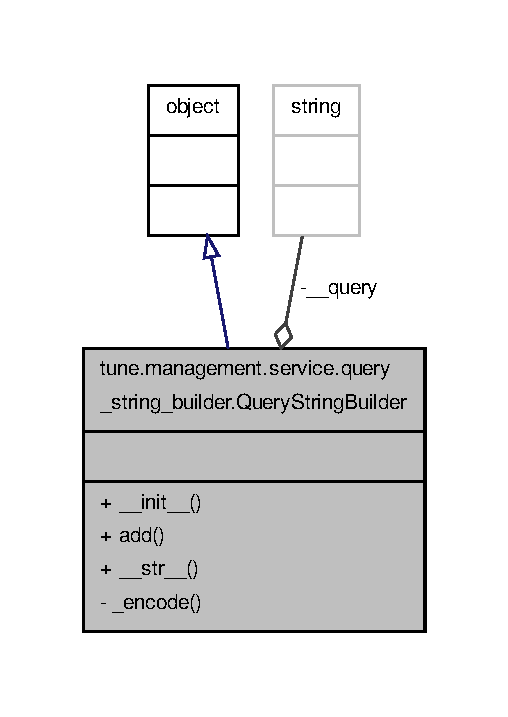
\includegraphics[width=244pt]{classtune_1_1management_1_1service_1_1query__string__builder_1_1QueryStringBuilder__coll__graph}
\end{center}
\end{figure}
\subsection*{Public Member Functions}
\begin{DoxyCompactItemize}
\item 
def \hyperlink{classtune_1_1management_1_1service_1_1query__string__builder_1_1QueryStringBuilder_a6364c0e70322f6fd9fc6446285fb916f}{\-\_\-\-\_\-init\-\_\-\-\_\-}
\begin{DoxyCompactList}\small\item\em Constructor a query string builder. \end{DoxyCompactList}\item 
def \hyperlink{classtune_1_1management_1_1service_1_1query__string__builder_1_1QueryStringBuilder_a52936a3c60cbe5dc990ece2561c4d69e}{add}
\begin{DoxyCompactList}\small\item\em Add query string parameter. \end{DoxyCompactList}\item 
def \hyperlink{classtune_1_1management_1_1service_1_1query__string__builder_1_1QueryStringBuilder_a7239f3a1db6e6d797aa07867b1029b21}{\-\_\-\-\_\-str\-\_\-\-\_\-}
\begin{DoxyCompactList}\small\item\em String representation of an object. \end{DoxyCompactList}\end{DoxyCompactItemize}
\subsection*{Private Member Functions}
\begin{DoxyCompactItemize}
\item 
def \hyperlink{classtune_1_1management_1_1service_1_1query__string__builder_1_1QueryStringBuilder_a0b965e40a56591054bb62d0178bbe8b9}{\-\_\-encode}
\begin{DoxyCompactList}\small\item\em U\-R\-L Encode query string parameter. \end{DoxyCompactList}\end{DoxyCompactItemize}
\subsection*{Static Private Attributes}
\begin{DoxyCompactItemize}
\item 
string \hyperlink{classtune_1_1management_1_1service_1_1query__string__builder_1_1QueryStringBuilder_a51080f1efb7e53b5df7c2ee223f73660}{\-\_\-\-\_\-query} = \char`\"{}\char`\"{}
\end{DoxyCompactItemize}


\subsection{Detailed Description}
Build Query String provide with dictionary of query parameters. 



Definition at line 55 of file query\-\_\-string\-\_\-builder.\-py.



\subsection{Constructor \& Destructor Documentation}
\hypertarget{classtune_1_1management_1_1service_1_1query__string__builder_1_1QueryStringBuilder_a6364c0e70322f6fd9fc6446285fb916f}{\index{tune\-::management\-::service\-::query\-\_\-string\-\_\-builder\-::\-Query\-String\-Builder@{tune\-::management\-::service\-::query\-\_\-string\-\_\-builder\-::\-Query\-String\-Builder}!\-\_\-\-\_\-init\-\_\-\-\_\-@{\-\_\-\-\_\-init\-\_\-\-\_\-}}
\index{\-\_\-\-\_\-init\-\_\-\-\_\-@{\-\_\-\-\_\-init\-\_\-\-\_\-}!tune::management::service::query_string_builder::QueryStringBuilder@{tune\-::management\-::service\-::query\-\_\-string\-\_\-builder\-::\-Query\-String\-Builder}}
\subsubsection[{\-\_\-\-\_\-init\-\_\-\-\_\-}]{\setlength{\rightskip}{0pt plus 5cm}def tune.\-management.\-service.\-query\-\_\-string\-\_\-builder.\-Query\-String\-Builder.\-\_\-\-\_\-init\-\_\-\-\_\- (
\begin{DoxyParamCaption}
\item[{}]{self, }
\item[{}]{name = {\ttfamily None}, }
\item[{}]{value = {\ttfamily None}}
\end{DoxyParamCaption}
)}}\label{classtune_1_1management_1_1service_1_1query__string__builder_1_1QueryStringBuilder_a6364c0e70322f6fd9fc6446285fb916f}


Constructor a query string builder. 

Args\-: name (str, optional)\-: query string parameter's key.\par
 value (str, optional)\-: query string parameter's value.\par


Definition at line 66 of file query\-\_\-string\-\_\-builder.\-py.


\begin{DoxyCode}
66 
67     \textcolor{keyword}{def }\hyperlink{classtune_1_1management_1_1service_1_1query__string__builder_1_1QueryStringBuilder_a6364c0e70322f6fd9fc6446285fb916f}{\_\_init\_\_}(self, name=None, value=None):
68         \textcolor{keywordflow}{if} name \textcolor{keywordflow}{is} \textcolor{keywordflow}{not} \textcolor{keywordtype}{None} \textcolor{keywordflow}{and} isinstance(name, str) \textcolor{keywordflow}{and} len(name) > 0:
69             self.\hyperlink{classtune_1_1management_1_1service_1_1query__string__builder_1_1QueryStringBuilder_a52936a3c60cbe5dc990ece2561c4d69e}{add}(name, value)

\end{DoxyCode}


Here is the call graph for this function\-:
\nopagebreak
\begin{figure}[H]
\begin{center}
\leavevmode
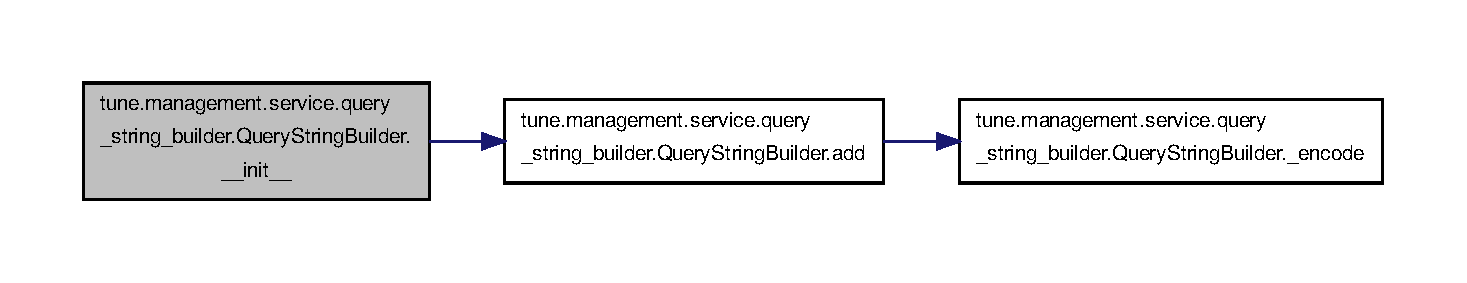
\includegraphics[width=350pt]{classtune_1_1management_1_1service_1_1query__string__builder_1_1QueryStringBuilder_a6364c0e70322f6fd9fc6446285fb916f_cgraph}
\end{center}
\end{figure}




\subsection{Member Function Documentation}
\hypertarget{classtune_1_1management_1_1service_1_1query__string__builder_1_1QueryStringBuilder_a7239f3a1db6e6d797aa07867b1029b21}{\index{tune\-::management\-::service\-::query\-\_\-string\-\_\-builder\-::\-Query\-String\-Builder@{tune\-::management\-::service\-::query\-\_\-string\-\_\-builder\-::\-Query\-String\-Builder}!\-\_\-\-\_\-str\-\_\-\-\_\-@{\-\_\-\-\_\-str\-\_\-\-\_\-}}
\index{\-\_\-\-\_\-str\-\_\-\-\_\-@{\-\_\-\-\_\-str\-\_\-\-\_\-}!tune::management::service::query_string_builder::QueryStringBuilder@{tune\-::management\-::service\-::query\-\_\-string\-\_\-builder\-::\-Query\-String\-Builder}}
\subsubsection[{\-\_\-\-\_\-str\-\_\-\-\_\-}]{\setlength{\rightskip}{0pt plus 5cm}def tune.\-management.\-service.\-query\-\_\-string\-\_\-builder.\-Query\-String\-Builder.\-\_\-\-\_\-str\-\_\-\-\_\- (
\begin{DoxyParamCaption}
\item[{}]{self}
\end{DoxyParamCaption}
)}}\label{classtune_1_1management_1_1service_1_1query__string__builder_1_1QueryStringBuilder_a7239f3a1db6e6d797aa07867b1029b21}


String representation of an object. 



Definition at line 173 of file query\-\_\-string\-\_\-builder.\-py.


\begin{DoxyCode}
173 
174     \textcolor{keyword}{def }\hyperlink{classtune_1_1management_1_1service_1_1query__string__builder_1_1QueryStringBuilder_a7239f3a1db6e6d797aa07867b1029b21}{\_\_str\_\_}(self):
175         \textcolor{keywordflow}{return} self.\hyperlink{classtune_1_1management_1_1service_1_1query__string__builder_1_1QueryStringBuilder_a51080f1efb7e53b5df7c2ee223f73660}{\_\_query}
\end{DoxyCode}
\hypertarget{classtune_1_1management_1_1service_1_1query__string__builder_1_1QueryStringBuilder_a0b965e40a56591054bb62d0178bbe8b9}{\index{tune\-::management\-::service\-::query\-\_\-string\-\_\-builder\-::\-Query\-String\-Builder@{tune\-::management\-::service\-::query\-\_\-string\-\_\-builder\-::\-Query\-String\-Builder}!\-\_\-encode@{\-\_\-encode}}
\index{\-\_\-encode@{\-\_\-encode}!tune::management::service::query_string_builder::QueryStringBuilder@{tune\-::management\-::service\-::query\-\_\-string\-\_\-builder\-::\-Query\-String\-Builder}}
\subsubsection[{\-\_\-encode}]{\setlength{\rightskip}{0pt plus 5cm}def tune.\-management.\-service.\-query\-\_\-string\-\_\-builder.\-Query\-String\-Builder.\-\_\-encode (
\begin{DoxyParamCaption}
\item[{}]{self, }
\item[{}]{name, }
\item[{}]{value}
\end{DoxyParamCaption}
)\hspace{0.3cm}{\ttfamily [private]}}}\label{classtune_1_1management_1_1service_1_1query__string__builder_1_1QueryStringBuilder_a0b965e40a56591054bb62d0178bbe8b9}


U\-R\-L Encode query string parameter. 

Args\-: name (str)\-: query string parameter's key.\par
 value (str)\-: query string parameter's value.\par


Definition at line 154 of file query\-\_\-string\-\_\-builder.\-py.


\begin{DoxyCode}
154 
155     \textcolor{keyword}{def }\hyperlink{classtune_1_1management_1_1service_1_1query__string__builder_1_1QueryStringBuilder_a0b965e40a56591054bb62d0178bbe8b9}{\_encode}(self, name, value):
156         \textcolor{keywordflow}{try}:
157             \textcolor{keywordflow}{if} self.\hyperlink{classtune_1_1management_1_1service_1_1query__string__builder_1_1QueryStringBuilder_a51080f1efb7e53b5df7c2ee223f73660}{\_\_query}:
158                 self.\hyperlink{classtune_1_1management_1_1service_1_1query__string__builder_1_1QueryStringBuilder_a51080f1efb7e53b5df7c2ee223f73660}{\_\_query} += \textcolor{stringliteral}{"&"}
159 
160             param = urllib.parse.urlencode(\{name : value\})
161             self.\hyperlink{classtune_1_1management_1_1service_1_1query__string__builder_1_1QueryStringBuilder_a51080f1efb7e53b5df7c2ee223f73660}{\_\_query} += param
162         \textcolor{keywordflow}{except} Exception \textcolor{keyword}{as} ex:
163             \textcolor{keywordflow}{raise} TuneSdkException(
164                 \textcolor{stringliteral}{"Failed to URL encode \{\}:\{\}: (\{0\})"}.format(
165                     name,
166                     value,
167                     str(ex)
168                     ),
169                 ex
170             )

\end{DoxyCode}


Here is the caller graph for this function\-:
\nopagebreak
\begin{figure}[H]
\begin{center}
\leavevmode
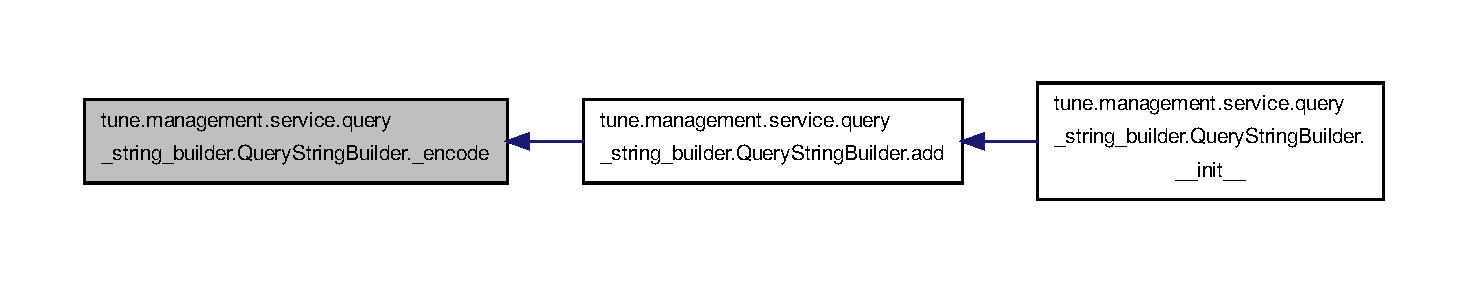
\includegraphics[width=350pt]{classtune_1_1management_1_1service_1_1query__string__builder_1_1QueryStringBuilder_a0b965e40a56591054bb62d0178bbe8b9_icgraph}
\end{center}
\end{figure}


\hypertarget{classtune_1_1management_1_1service_1_1query__string__builder_1_1QueryStringBuilder_a52936a3c60cbe5dc990ece2561c4d69e}{\index{tune\-::management\-::service\-::query\-\_\-string\-\_\-builder\-::\-Query\-String\-Builder@{tune\-::management\-::service\-::query\-\_\-string\-\_\-builder\-::\-Query\-String\-Builder}!add@{add}}
\index{add@{add}!tune::management::service::query_string_builder::QueryStringBuilder@{tune\-::management\-::service\-::query\-\_\-string\-\_\-builder\-::\-Query\-String\-Builder}}
\subsubsection[{add}]{\setlength{\rightskip}{0pt plus 5cm}def tune.\-management.\-service.\-query\-\_\-string\-\_\-builder.\-Query\-String\-Builder.\-add (
\begin{DoxyParamCaption}
\item[{}]{self, }
\item[{}]{name, }
\item[{}]{value}
\end{DoxyParamCaption}
)}}\label{classtune_1_1management_1_1service_1_1query__string__builder_1_1QueryStringBuilder_a52936a3c60cbe5dc990ece2561c4d69e}


Add query string parameter. 

Args\-: name (str)\-: query string parameter's key.\par
 value (str)\-: query string parameter's value.\par


Definition at line 77 of file query\-\_\-string\-\_\-builder.\-py.


\begin{DoxyCode}
77 
78     \textcolor{keyword}{def }\hyperlink{classtune_1_1management_1_1service_1_1query__string__builder_1_1QueryStringBuilder_a52936a3c60cbe5dc990ece2561c4d69e}{add}(self, name, value):
79         \textcolor{keywordflow}{if} value \textcolor{keywordflow}{is} \textcolor{keywordtype}{None}:
80             \textcolor{keywordflow}{return}
81 
82         \textcolor{keywordflow}{if} \textcolor{keywordflow}{not} name \textcolor{keywordflow}{or} \textcolor{keywordflow}{not} isinstance(name, str):
83             \textcolor{keywordflow}{raise} ValueError(\textcolor{stringliteral}{"Parameter 'name' is not defined."})
84 
85         name = name.strip()
86 
87         \textcolor{keywordflow}{if} len(name) < 1:
88             \textcolor{keywordflow}{raise} ValueError(\textcolor{stringliteral}{"Parameter 'name' is not defined."})
89 
90         \textcolor{keywordflow}{if} isinstance(value, str):
91             value = value.strip()
92             \textcolor{keywordflow}{if} len(value) < 1:
93                 \textcolor{keywordflow}{return}
94 
95         \textcolor{keywordflow}{try}:
96             \textcolor{keywordflow}{if} name == \textcolor{stringliteral}{"fields"}:
97                 \textcolor{comment}{# Remove all spaces}
98                 fields\_value = re.sub(\textcolor{stringliteral}{r'\(\backslash\)s+'}, \textcolor{stringliteral}{''}, value)
99 
100                 self.\hyperlink{classtune_1_1management_1_1service_1_1query__string__builder_1_1QueryStringBuilder_a0b965e40a56591054bb62d0178bbe8b9}{\_encode}(name, fields\_value)
101 
102             \textcolor{keywordflow}{elif} name == \textcolor{stringliteral}{"sort"}:
103                 \textcolor{keywordflow}{if} type(value) \textcolor{keywordflow}{is} \textcolor{keywordflow}{not} dict:
104                     \textcolor{keywordflow}{raise} ValueError(\textcolor{stringliteral}{"Parameter 'sort' value is not a dictionary."})
105 
106                 \textcolor{keywordflow}{for} sort\_field, sort\_direction \textcolor{keywordflow}{in} value.items():
107                     sort\_direction = sort\_direction.upper()
108                     \textcolor{keywordflow}{if} sort\_direction != \textcolor{stringliteral}{"ASC"} \textcolor{keywordflow}{and} sort\_direction != \textcolor{stringliteral}{"DESC"}:
109                         \textcolor{keywordflow}{raise} ValueError(\textcolor{stringliteral}{"Parameter 'sort' has invalid direction: '\{\}'"}.format(
110                             sort\_direction
111                             )
112                         )
113                     sort\_name = \textcolor{stringliteral}{"sort[\{\}]"}.format(sort\_field)
114                     sort\_value = sort\_direction
115                     self.\hyperlink{classtune_1_1management_1_1service_1_1query__string__builder_1_1QueryStringBuilder_a0b965e40a56591054bb62d0178bbe8b9}{\_encode}(sort\_name, sort\_value)
116 
117             \textcolor{keywordflow}{elif} name == \textcolor{stringliteral}{"filter"}:
118                 filter\_value = re.sub(\textcolor{stringliteral}{r'\(\backslash\)s+'}, \textcolor{stringliteral}{' '}, value)
119 
120                 self.\hyperlink{classtune_1_1management_1_1service_1_1query__string__builder_1_1QueryStringBuilder_a0b965e40a56591054bb62d0178bbe8b9}{\_encode}(name, filter\_value)
121 
122             \textcolor{keywordflow}{elif} name == \textcolor{stringliteral}{"group"}:
123                 group\_value = re.sub(\textcolor{stringliteral}{r'\(\backslash\)s+'}, \textcolor{stringliteral}{''}, value)
124 
125                 self.\hyperlink{classtune_1_1management_1_1service_1_1query__string__builder_1_1QueryStringBuilder_a0b965e40a56591054bb62d0178bbe8b9}{\_encode}(name, group\_value)
126 
127             \textcolor{keywordflow}{elif} isinstance(value, bool):
128                 \textcolor{keywordflow}{if} value == \textcolor{keyword}{False}:
129                     bool\_value = \textcolor{stringliteral}{"false"}
130                 \textcolor{keywordflow}{elif} value == \textcolor{keyword}{True}:
131                     bool\_value = \textcolor{stringliteral}{"true"}
132 
133                 self.\hyperlink{classtune_1_1management_1_1service_1_1query__string__builder_1_1QueryStringBuilder_a0b965e40a56591054bb62d0178bbe8b9}{\_encode}(name, bool\_value)
134 
135             \textcolor{keywordflow}{else}:
136 
137                 self.\hyperlink{classtune_1_1management_1_1service_1_1query__string__builder_1_1QueryStringBuilder_a0b965e40a56591054bb62d0178bbe8b9}{\_encode}(name, value)
138         \textcolor{keywordflow}{except} Exception \textcolor{keyword}{as} ex:
139             \textcolor{keywordflow}{raise} TuneSdkException(
140                 \textcolor{stringliteral}{"Failed to add query string parameter (\{0\},\{1\}): \{2\}"}.format(
141                     name,
142                     value,
143                     str(ex)
144                     ),
145                 ex
146             )

\end{DoxyCode}


Here is the call graph for this function\-:
\nopagebreak
\begin{figure}[H]
\begin{center}
\leavevmode
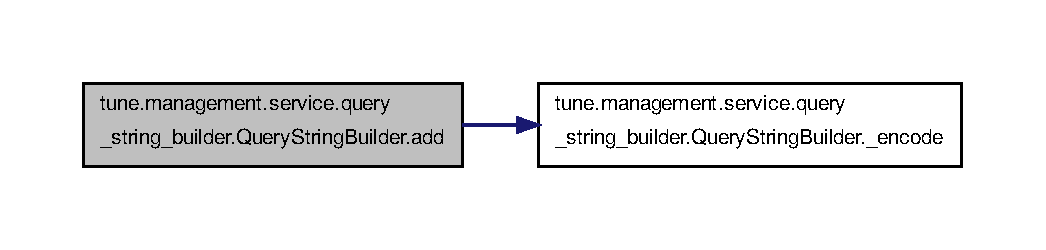
\includegraphics[width=350pt]{classtune_1_1management_1_1service_1_1query__string__builder_1_1QueryStringBuilder_a52936a3c60cbe5dc990ece2561c4d69e_cgraph}
\end{center}
\end{figure}




Here is the caller graph for this function\-:
\nopagebreak
\begin{figure}[H]
\begin{center}
\leavevmode
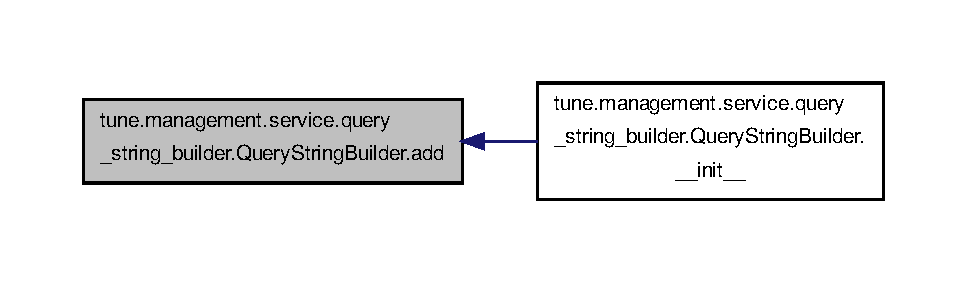
\includegraphics[width=350pt]{classtune_1_1management_1_1service_1_1query__string__builder_1_1QueryStringBuilder_a52936a3c60cbe5dc990ece2561c4d69e_icgraph}
\end{center}
\end{figure}




\subsection{Member Data Documentation}
\hypertarget{classtune_1_1management_1_1service_1_1query__string__builder_1_1QueryStringBuilder_a51080f1efb7e53b5df7c2ee223f73660}{\index{tune\-::management\-::service\-::query\-\_\-string\-\_\-builder\-::\-Query\-String\-Builder@{tune\-::management\-::service\-::query\-\_\-string\-\_\-builder\-::\-Query\-String\-Builder}!\-\_\-\-\_\-query@{\-\_\-\-\_\-query}}
\index{\-\_\-\-\_\-query@{\-\_\-\-\_\-query}!tune::management::service::query_string_builder::QueryStringBuilder@{tune\-::management\-::service\-::query\-\_\-string\-\_\-builder\-::\-Query\-String\-Builder}}
\subsubsection[{\-\_\-\-\_\-query}]{\setlength{\rightskip}{0pt plus 5cm}string tune.\-management.\-service.\-query\-\_\-string\-\_\-builder.\-Query\-String\-Builder.\-\_\-\-\_\-query = \char`\"{}\char`\"{}\hspace{0.3cm}{\ttfamily [static]}, {\ttfamily [private]}}}\label{classtune_1_1management_1_1service_1_1query__string__builder_1_1QueryStringBuilder_a51080f1efb7e53b5df7c2ee223f73660}


Definition at line 57 of file query\-\_\-string\-\_\-builder.\-py.



The documentation for this class was generated from the following file\-:\begin{DoxyCompactItemize}
\item 
tune/management/service/\hyperlink{query__string__builder_8py}{query\-\_\-string\-\_\-builder.\-py}\end{DoxyCompactItemize}

\hypertarget{classtune_1_1management_1_1reports_1_1report__export__worker_1_1ReportExportWorker}{\section{tune.\-management.\-reports.\-report\-\_\-export\-\_\-worker.\-Report\-Export\-Worker Class Reference}
\label{classtune_1_1management_1_1reports_1_1report__export__worker_1_1ReportExportWorker}\index{tune.\-management.\-reports.\-report\-\_\-export\-\_\-worker.\-Report\-Export\-Worker@{tune.\-management.\-reports.\-report\-\_\-export\-\_\-worker.\-Report\-Export\-Worker}}
}


Threaded worker for handle polling of report request on export queue.  




Inheritance diagram for tune.\-management.\-reports.\-report\-\_\-export\-\_\-worker.\-Report\-Export\-Worker\-:
\nopagebreak
\begin{figure}[H]
\begin{center}
\leavevmode
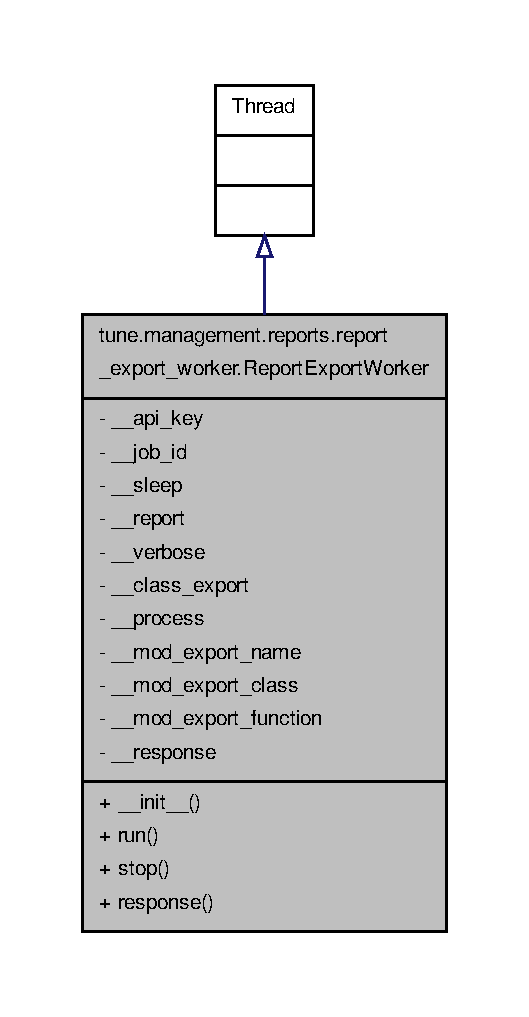
\includegraphics[width=254pt]{classtune_1_1management_1_1reports_1_1report__export__worker_1_1ReportExportWorker__inherit__graph}
\end{center}
\end{figure}


Collaboration diagram for tune.\-management.\-reports.\-report\-\_\-export\-\_\-worker.\-Report\-Export\-Worker\-:
\nopagebreak
\begin{figure}[H]
\begin{center}
\leavevmode
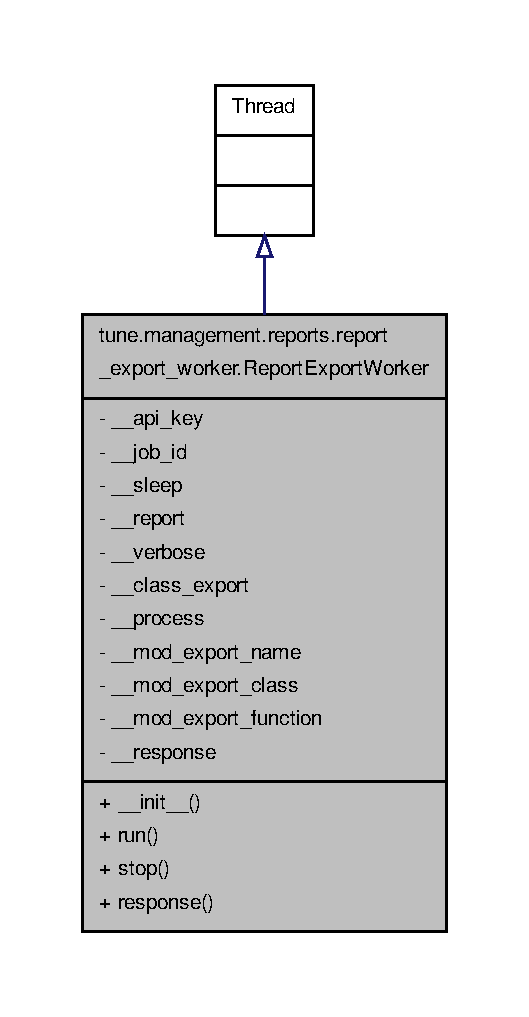
\includegraphics[width=254pt]{classtune_1_1management_1_1reports_1_1report__export__worker_1_1ReportExportWorker__coll__graph}
\end{center}
\end{figure}
\subsection*{Public Member Functions}
\begin{DoxyCompactItemize}
\item 
def \hyperlink{classtune_1_1management_1_1reports_1_1report__export__worker_1_1ReportExportWorker_a499f66d898085a548f1ac4fbe7987751}{\-\_\-\-\_\-init\-\_\-\-\_\-}
\begin{DoxyCompactList}\small\item\em The constructor. \end{DoxyCompactList}\item 
def \hyperlink{classtune_1_1management_1_1reports_1_1report__export__worker_1_1ReportExportWorker_a44d3b02f06bbe340a4311e84a28055ac}{run}
\begin{DoxyCompactList}\small\item\em Poll export for download U\-R\-L. \end{DoxyCompactList}\item 
def \hyperlink{classtune_1_1management_1_1reports_1_1report__export__worker_1_1ReportExportWorker_a448cbf72ff829120b72294d038025548}{stop}
\begin{DoxyCompactList}\small\item\em Terminate thread. \end{DoxyCompactList}\item 
def \hyperlink{classtune_1_1management_1_1reports_1_1report__export__worker_1_1ReportExportWorker_ab802b6d34e51728b8fce42fc8910a02c}{response}
\begin{DoxyCompactList}\small\item\em Property that will hold completed report downloaded from Management A\-P\-I service. \end{DoxyCompactList}\end{DoxyCompactItemize}
\subsection*{Private Attributes}
\begin{DoxyCompactItemize}
\item 
\hyperlink{classtune_1_1management_1_1reports_1_1report__export__worker_1_1ReportExportWorker_af497eaf63b74b36fb52c624c4cd3ed69}{\-\_\-\-\_\-api\-\_\-key}
\item 
\hyperlink{classtune_1_1management_1_1reports_1_1report__export__worker_1_1ReportExportWorker_a5360619387f156dd92ebf971b5353047}{\-\_\-\-\_\-job\-\_\-id}
\item 
\hyperlink{classtune_1_1management_1_1reports_1_1report__export__worker_1_1ReportExportWorker_af49d9582e87d273aeb98dd89fdddd6ef}{\-\_\-\-\_\-sleep}
\item 
\hyperlink{classtune_1_1management_1_1reports_1_1report__export__worker_1_1ReportExportWorker_a010bd4cacd16b8ed1b16d5a87c0b80ac}{\-\_\-\-\_\-report}
\item 
\hyperlink{classtune_1_1management_1_1reports_1_1report__export__worker_1_1ReportExportWorker_a06a086d2025a26d725ed44f0d3340c7a}{\-\_\-\-\_\-verbose}
\item 
\hyperlink{classtune_1_1management_1_1reports_1_1report__export__worker_1_1ReportExportWorker_a398025eb4319898a002a2996e9e12e55}{\-\_\-\-\_\-class\-\_\-export}
\item 
\hyperlink{classtune_1_1management_1_1reports_1_1report__export__worker_1_1ReportExportWorker_afbdedb366ee3e00378979a90bac67bb8}{\-\_\-\-\_\-process}
\item 
\hyperlink{classtune_1_1management_1_1reports_1_1report__export__worker_1_1ReportExportWorker_a91eca8e3ded9a6c9de6178e3d79a4aef}{\-\_\-\-\_\-mod\-\_\-export\-\_\-name}
\item 
\hyperlink{classtune_1_1management_1_1reports_1_1report__export__worker_1_1ReportExportWorker_a4c386593ffcdd04855e2ab55112c7c92}{\-\_\-\-\_\-mod\-\_\-export\-\_\-class}
\item 
\hyperlink{classtune_1_1management_1_1reports_1_1report__export__worker_1_1ReportExportWorker_a817a81e441f511cd5464c5e9358d4d59}{\-\_\-\-\_\-mod\-\_\-export\-\_\-function}
\item 
\hyperlink{classtune_1_1management_1_1reports_1_1report__export__worker_1_1ReportExportWorker_a5b667fc3fb9be24b55282e0ef26671b1}{\-\_\-\-\_\-response}
\end{DoxyCompactItemize}


\subsection{Detailed Description}
Threaded worker for handle polling of report request on export queue. 

Definition at line 59 of file report\-\_\-export\-\_\-worker.\-py.



\subsection{Constructor \& Destructor Documentation}
\hypertarget{classtune_1_1management_1_1reports_1_1report__export__worker_1_1ReportExportWorker_a499f66d898085a548f1ac4fbe7987751}{\index{tune\-::management\-::reports\-::report\-\_\-export\-\_\-worker\-::\-Report\-Export\-Worker@{tune\-::management\-::reports\-::report\-\_\-export\-\_\-worker\-::\-Report\-Export\-Worker}!\-\_\-\-\_\-init\-\_\-\-\_\-@{\-\_\-\-\_\-init\-\_\-\-\_\-}}
\index{\-\_\-\-\_\-init\-\_\-\-\_\-@{\-\_\-\-\_\-init\-\_\-\-\_\-}!tune::management::reports::report_export_worker::ReportExportWorker@{tune\-::management\-::reports\-::report\-\_\-export\-\_\-worker\-::\-Report\-Export\-Worker}}
\subsubsection[{\-\_\-\-\_\-init\-\_\-\-\_\-}]{\setlength{\rightskip}{0pt plus 5cm}def tune.\-management.\-reports.\-report\-\_\-export\-\_\-worker.\-Report\-Export\-Worker.\-\_\-\-\_\-init\-\_\-\-\_\- (
\begin{DoxyParamCaption}
\item[{}]{self, }
\item[{}]{mod\-\_\-export\-\_\-namespace, }
\item[{}]{mod\-\_\-export\-\_\-class, }
\item[{}]{mod\-\_\-export\-\_\-function, }
\item[{}]{api\-\_\-key, }
\item[{}]{job\-\_\-id, }
\item[{}]{verbose = {\ttfamily False}, }
\item[{}]{sleep = {\ttfamily 60~\#~seconds}}
\end{DoxyParamCaption}
)}}\label{classtune_1_1management_1_1reports_1_1report__export__worker_1_1ReportExportWorker_a499f66d898085a548f1ac4fbe7987751}


The constructor. 


\begin{DoxyParams}{Parameters}
{\em string} & mod\-\_\-export\-\_\-class Reference class name for worker to perform download status query. \\
\hline
{\em string} & mod\-\_\-export\-\_\-function Reference class function name for worker to perform download status query. \\
\hline
{\em string} & api\-\_\-key Mobile\-App\-Tracking A\-P\-I Key \\
\hline
{\em string} & job\-\_\-id Provided Job Identifier to reference requested report on export queue. \\
\hline
{\em bool} & verbose Debug purposes only to view progress of job on export queue. \\
\hline
{\em int} & sleep Polling delay between querying job status on export queue. \\
\hline
\end{DoxyParams}


Definition at line 83 of file report\-\_\-export\-\_\-worker.\-py.


\begin{DoxyCode}
83 
84          ):
85         \textcolor{comment}{# api\_key}
86         \textcolor{keywordflow}{if} \textcolor{keywordflow}{not} api\_key \textcolor{keywordflow}{or} len(api\_key) < 1:
87             \textcolor{keywordflow}{raise} ValueError(\textcolor{stringliteral}{"Parameter 'api\_key' is not defined."})
88 
89         \textcolor{comment}{# job\_id}
90         \textcolor{keywordflow}{if} \textcolor{keywordflow}{not} job\_id \textcolor{keywordflow}{or} len(job\_id) < 1:
91             \textcolor{keywordflow}{raise} ValueError(\textcolor{stringliteral}{"Parameter 'job\_id' is not defined."})
92 
93         loaded\_mod = \_\_import\_\_(mod\_export\_namespace, fromlist=[mod\_export\_namespace])
94 
95         \textcolor{comment}{# Load it from imported module}
96         loaded\_class = getattr(loaded\_mod, mod\_export\_class)
97 
98         \textcolor{comment}{# Create an instance of it}
99         instance = loaded\_class(api\_key)
100 
101         Thread.\_\_init\_\_(self)
102         self.\hyperlink{classtune_1_1management_1_1reports_1_1report__export__worker_1_1ReportExportWorker_af497eaf63b74b36fb52c624c4cd3ed69}{\_\_api\_key} = api\_key
103         self.\hyperlink{classtune_1_1management_1_1reports_1_1report__export__worker_1_1ReportExportWorker_a5360619387f156dd92ebf971b5353047}{\_\_job\_id} = job\_id
104         self.\hyperlink{classtune_1_1management_1_1reports_1_1report__export__worker_1_1ReportExportWorker_af49d9582e87d273aeb98dd89fdddd6ef}{\_\_sleep} = sleep
105         self.\hyperlink{classtune_1_1management_1_1reports_1_1report__export__worker_1_1ReportExportWorker_a010bd4cacd16b8ed1b16d5a87c0b80ac}{\_\_report} = \textcolor{keywordtype}{None}
106         self.\hyperlink{classtune_1_1management_1_1reports_1_1report__export__worker_1_1ReportExportWorker_a06a086d2025a26d725ed44f0d3340c7a}{\_\_verbose} = verbose
107         self.\hyperlink{classtune_1_1management_1_1reports_1_1report__export__worker_1_1ReportExportWorker_a398025eb4319898a002a2996e9e12e55}{\_\_class\_export} = instance
108         self.\hyperlink{classtune_1_1management_1_1reports_1_1report__export__worker_1_1ReportExportWorker_afbdedb366ee3e00378979a90bac67bb8}{\_\_process} = \textcolor{keywordtype}{None}
109         self.\hyperlink{classtune_1_1management_1_1reports_1_1report__export__worker_1_1ReportExportWorker_a91eca8e3ded9a6c9de6178e3d79a4aef}{\_\_mod\_export\_name} = mod\_export\_namespace
110         self.\hyperlink{classtune_1_1management_1_1reports_1_1report__export__worker_1_1ReportExportWorker_a4c386593ffcdd04855e2ab55112c7c92}{\_\_mod\_export\_class} = mod\_export\_class
111         self.\hyperlink{classtune_1_1management_1_1reports_1_1report__export__worker_1_1ReportExportWorker_a817a81e441f511cd5464c5e9358d4d59}{\_\_mod\_export\_function} = mod\_export\_function
112         self.\hyperlink{classtune_1_1management_1_1reports_1_1report__export__worker_1_1ReportExportWorker_a5b667fc3fb9be24b55282e0ef26671b1}{\_\_response} = \textcolor{keywordtype}{None}

\end{DoxyCode}


\subsection{Member Function Documentation}
\hypertarget{classtune_1_1management_1_1reports_1_1report__export__worker_1_1ReportExportWorker_ab802b6d34e51728b8fce42fc8910a02c}{\index{tune\-::management\-::reports\-::report\-\_\-export\-\_\-worker\-::\-Report\-Export\-Worker@{tune\-::management\-::reports\-::report\-\_\-export\-\_\-worker\-::\-Report\-Export\-Worker}!response@{response}}
\index{response@{response}!tune::management::reports::report_export_worker::ReportExportWorker@{tune\-::management\-::reports\-::report\-\_\-export\-\_\-worker\-::\-Report\-Export\-Worker}}
\subsubsection[{response}]{\setlength{\rightskip}{0pt plus 5cm}def tune.\-management.\-reports.\-report\-\_\-export\-\_\-worker.\-Report\-Export\-Worker.\-response (
\begin{DoxyParamCaption}
\item[{}]{self}
\end{DoxyParamCaption}
)}}\label{classtune_1_1management_1_1reports_1_1report__export__worker_1_1ReportExportWorker_ab802b6d34e51728b8fce42fc8910a02c}


Property that will hold completed report downloaded from Management A\-P\-I service. 



Definition at line 189 of file report\-\_\-export\-\_\-worker.\-py.


\begin{DoxyCode}
189 
190     \textcolor{keyword}{def }\hyperlink{classtune_1_1management_1_1reports_1_1report__export__worker_1_1ReportExportWorker_ab802b6d34e51728b8fce42fc8910a02c}{response}(self):
191         \textcolor{keywordflow}{return} self.\hyperlink{classtune_1_1management_1_1reports_1_1report__export__worker_1_1ReportExportWorker_a5b667fc3fb9be24b55282e0ef26671b1}{\_\_response}
\end{DoxyCode}
\hypertarget{classtune_1_1management_1_1reports_1_1report__export__worker_1_1ReportExportWorker_a44d3b02f06bbe340a4311e84a28055ac}{\index{tune\-::management\-::reports\-::report\-\_\-export\-\_\-worker\-::\-Report\-Export\-Worker@{tune\-::management\-::reports\-::report\-\_\-export\-\_\-worker\-::\-Report\-Export\-Worker}!run@{run}}
\index{run@{run}!tune::management::reports::report_export_worker::ReportExportWorker@{tune\-::management\-::reports\-::report\-\_\-export\-\_\-worker\-::\-Report\-Export\-Worker}}
\subsubsection[{run}]{\setlength{\rightskip}{0pt plus 5cm}def tune.\-management.\-reports.\-report\-\_\-export\-\_\-worker.\-Report\-Export\-Worker.\-run (
\begin{DoxyParamCaption}
\item[{}]{self}
\end{DoxyParamCaption}
)}}\label{classtune_1_1management_1_1reports_1_1report__export__worker_1_1ReportExportWorker_a44d3b02f06bbe340a4311e84a28055ac}


Poll export for download U\-R\-L. 

Method representing the thread's activity. 

Definition at line 116 of file report\-\_\-export\-\_\-worker.\-py.


\begin{DoxyCode}
116 
117     \textcolor{keyword}{def }\hyperlink{classtune_1_1management_1_1reports_1_1report__export__worker_1_1ReportExportWorker_a44d3b02f06bbe340a4311e84a28055ac}{run}(self):
118         cmd = [\textcolor{stringliteral}{"bash"}, \textcolor{stringliteral}{'process.sh'}]
119         self.\hyperlink{classtune_1_1management_1_1reports_1_1report__export__worker_1_1ReportExportWorker_afbdedb366ee3e00378979a90bac67bb8}{\_\_process} = subprocess.Popen(cmd,
120                      stdout=subprocess.PIPE,
121                      stderr=subprocess.STDOUT)
122         status = \textcolor{stringliteral}{"running"}
123         response = \textcolor{keywordtype}{None}
124         attempt = 0
125 
126         \textcolor{keywordflow}{while} \textcolor{keyword}{True}:
127             response = getattr(self.\hyperlink{classtune_1_1management_1_1reports_1_1report__export__worker_1_1ReportExportWorker_a398025eb4319898a002a2996e9e12e55}{\_\_class\_export}, self.
      \hyperlink{classtune_1_1management_1_1reports_1_1report__export__worker_1_1ReportExportWorker_a817a81e441f511cd5464c5e9358d4d59}{\_\_mod\_export\_function})(
128                     self.\hyperlink{classtune_1_1management_1_1reports_1_1report__export__worker_1_1ReportExportWorker_a5360619387f156dd92ebf971b5353047}{\_\_job\_id}
129                 )
130 
131             \textcolor{keywordflow}{if} \textcolor{keywordflow}{not} response:
132                 \textcolor{keywordflow}{raise} TuneSdkException(
133                     \textcolor{stringliteral}{"No response returned from export request."}
134                 )
135 
136             \textcolor{keywordflow}{if} \textcolor{keywordflow}{not} response.data:
137                 \textcolor{keywordflow}{raise} TuneSdkException(
138                     \textcolor{stringliteral}{"No response data returned from export. Request URL: \{\}"}.format(
139                         response.request\_url
140                     )
141                 )
142 
143             \textcolor{keywordflow}{if} response.http\_code != 200:
144                 \textcolor{keywordflow}{raise} TuneServiceException(
145                     \textcolor{stringliteral}{"Request failed: HTTP Error Code: \{\}: \{\}"}.format(
146                         response.http\_code,
147                         response.request\_url
148                     )
149                 )
150 
151             status = response.data[\textcolor{stringliteral}{"status"}]
152             \textcolor{keywordflow}{if} status == \textcolor{stringliteral}{"complete"} \textcolor{keywordflow}{or} status == \textcolor{stringliteral}{"fail"}:
153                 \textcolor{keywordflow}{break}
154 
155             attempt += 1
156             \textcolor{keywordflow}{if} self.\hyperlink{classtune_1_1management_1_1reports_1_1report__export__worker_1_1ReportExportWorker_a06a086d2025a26d725ed44f0d3340c7a}{\_\_verbose}:
157                 print(\textcolor{stringliteral}{"= thread id \{\}: attempt: \{\}, response: \{\}"}.format(
158                         current\_thread().ident,
159                         attempt,
160                         response
161                     )
162                 )
163 
164             time.sleep(self.\hyperlink{classtune_1_1management_1_1reports_1_1report__export__worker_1_1ReportExportWorker_af49d9582e87d273aeb98dd89fdddd6ef}{\_\_sleep})
165 
166         \textcolor{keywordflow}{if} self.\hyperlink{classtune_1_1management_1_1reports_1_1report__export__worker_1_1ReportExportWorker_a06a086d2025a26d725ed44f0d3340c7a}{\_\_verbose}:
167             print(\textcolor{stringliteral}{"= thread id \{\}: response: \{\}"}.format(
168                     current\_thread().ident,
169                     response
170                 )
171             )
172 
173         self.\hyperlink{classtune_1_1management_1_1reports_1_1report__export__worker_1_1ReportExportWorker_a5b667fc3fb9be24b55282e0ef26671b1}{\_\_response} = response

\end{DoxyCode}
\hypertarget{classtune_1_1management_1_1reports_1_1report__export__worker_1_1ReportExportWorker_a448cbf72ff829120b72294d038025548}{\index{tune\-::management\-::reports\-::report\-\_\-export\-\_\-worker\-::\-Report\-Export\-Worker@{tune\-::management\-::reports\-::report\-\_\-export\-\_\-worker\-::\-Report\-Export\-Worker}!stop@{stop}}
\index{stop@{stop}!tune::management::reports::report_export_worker::ReportExportWorker@{tune\-::management\-::reports\-::report\-\_\-export\-\_\-worker\-::\-Report\-Export\-Worker}}
\subsubsection[{stop}]{\setlength{\rightskip}{0pt plus 5cm}def tune.\-management.\-reports.\-report\-\_\-export\-\_\-worker.\-Report\-Export\-Worker.\-stop (
\begin{DoxyParamCaption}
\item[{}]{self}
\end{DoxyParamCaption}
)}}\label{classtune_1_1management_1_1reports_1_1report__export__worker_1_1ReportExportWorker_a448cbf72ff829120b72294d038025548}


Terminate thread. 



Definition at line 176 of file report\-\_\-export\-\_\-worker.\-py.


\begin{DoxyCode}
176 
177     \textcolor{keyword}{def }\hyperlink{classtune_1_1management_1_1reports_1_1report__export__worker_1_1ReportExportWorker_a448cbf72ff829120b72294d038025548}{stop}(self):
178         \textcolor{keywordflow}{if} self.\hyperlink{classtune_1_1management_1_1reports_1_1report__export__worker_1_1ReportExportWorker_a06a086d2025a26d725ed44f0d3340c7a}{\_\_verbose}:
179             print(\textcolor{stringliteral}{"= \{\}: Trying to stop"}.format(current\_thread()))
180         \textcolor{keywordflow}{if} self.\hyperlink{classtune_1_1management_1_1reports_1_1report__export__worker_1_1ReportExportWorker_afbdedb366ee3e00378979a90bac67bb8}{\_\_process} \textcolor{keywordflow}{is} \textcolor{keywordflow}{not} \textcolor{keywordtype}{None}:
181             self.\_\_process.terminate()
182             self.\hyperlink{classtune_1_1management_1_1reports_1_1report__export__worker_1_1ReportExportWorker_afbdedb366ee3e00378979a90bac67bb8}{\_\_process} = \textcolor{keywordtype}{None}

\end{DoxyCode}


\subsection{Member Data Documentation}
\hypertarget{classtune_1_1management_1_1reports_1_1report__export__worker_1_1ReportExportWorker_af497eaf63b74b36fb52c624c4cd3ed69}{\index{tune\-::management\-::reports\-::report\-\_\-export\-\_\-worker\-::\-Report\-Export\-Worker@{tune\-::management\-::reports\-::report\-\_\-export\-\_\-worker\-::\-Report\-Export\-Worker}!\-\_\-\-\_\-api\-\_\-key@{\-\_\-\-\_\-api\-\_\-key}}
\index{\-\_\-\-\_\-api\-\_\-key@{\-\_\-\-\_\-api\-\_\-key}!tune::management::reports::report_export_worker::ReportExportWorker@{tune\-::management\-::reports\-::report\-\_\-export\-\_\-worker\-::\-Report\-Export\-Worker}}
\subsubsection[{\-\_\-\-\_\-api\-\_\-key}]{\setlength{\rightskip}{0pt plus 5cm}tune.\-management.\-reports.\-report\-\_\-export\-\_\-worker.\-Report\-Export\-Worker.\-\_\-\-\_\-api\-\_\-key\hspace{0.3cm}{\ttfamily [private]}}}\label{classtune_1_1management_1_1reports_1_1report__export__worker_1_1ReportExportWorker_af497eaf63b74b36fb52c624c4cd3ed69}


Definition at line 101 of file report\-\_\-export\-\_\-worker.\-py.

\hypertarget{classtune_1_1management_1_1reports_1_1report__export__worker_1_1ReportExportWorker_a398025eb4319898a002a2996e9e12e55}{\index{tune\-::management\-::reports\-::report\-\_\-export\-\_\-worker\-::\-Report\-Export\-Worker@{tune\-::management\-::reports\-::report\-\_\-export\-\_\-worker\-::\-Report\-Export\-Worker}!\-\_\-\-\_\-class\-\_\-export@{\-\_\-\-\_\-class\-\_\-export}}
\index{\-\_\-\-\_\-class\-\_\-export@{\-\_\-\-\_\-class\-\_\-export}!tune::management::reports::report_export_worker::ReportExportWorker@{tune\-::management\-::reports\-::report\-\_\-export\-\_\-worker\-::\-Report\-Export\-Worker}}
\subsubsection[{\-\_\-\-\_\-class\-\_\-export}]{\setlength{\rightskip}{0pt plus 5cm}tune.\-management.\-reports.\-report\-\_\-export\-\_\-worker.\-Report\-Export\-Worker.\-\_\-\-\_\-class\-\_\-export\hspace{0.3cm}{\ttfamily [private]}}}\label{classtune_1_1management_1_1reports_1_1report__export__worker_1_1ReportExportWorker_a398025eb4319898a002a2996e9e12e55}


Definition at line 106 of file report\-\_\-export\-\_\-worker.\-py.

\hypertarget{classtune_1_1management_1_1reports_1_1report__export__worker_1_1ReportExportWorker_a5360619387f156dd92ebf971b5353047}{\index{tune\-::management\-::reports\-::report\-\_\-export\-\_\-worker\-::\-Report\-Export\-Worker@{tune\-::management\-::reports\-::report\-\_\-export\-\_\-worker\-::\-Report\-Export\-Worker}!\-\_\-\-\_\-job\-\_\-id@{\-\_\-\-\_\-job\-\_\-id}}
\index{\-\_\-\-\_\-job\-\_\-id@{\-\_\-\-\_\-job\-\_\-id}!tune::management::reports::report_export_worker::ReportExportWorker@{tune\-::management\-::reports\-::report\-\_\-export\-\_\-worker\-::\-Report\-Export\-Worker}}
\subsubsection[{\-\_\-\-\_\-job\-\_\-id}]{\setlength{\rightskip}{0pt plus 5cm}tune.\-management.\-reports.\-report\-\_\-export\-\_\-worker.\-Report\-Export\-Worker.\-\_\-\-\_\-job\-\_\-id\hspace{0.3cm}{\ttfamily [private]}}}\label{classtune_1_1management_1_1reports_1_1report__export__worker_1_1ReportExportWorker_a5360619387f156dd92ebf971b5353047}


Definition at line 102 of file report\-\_\-export\-\_\-worker.\-py.

\hypertarget{classtune_1_1management_1_1reports_1_1report__export__worker_1_1ReportExportWorker_a4c386593ffcdd04855e2ab55112c7c92}{\index{tune\-::management\-::reports\-::report\-\_\-export\-\_\-worker\-::\-Report\-Export\-Worker@{tune\-::management\-::reports\-::report\-\_\-export\-\_\-worker\-::\-Report\-Export\-Worker}!\-\_\-\-\_\-mod\-\_\-export\-\_\-class@{\-\_\-\-\_\-mod\-\_\-export\-\_\-class}}
\index{\-\_\-\-\_\-mod\-\_\-export\-\_\-class@{\-\_\-\-\_\-mod\-\_\-export\-\_\-class}!tune::management::reports::report_export_worker::ReportExportWorker@{tune\-::management\-::reports\-::report\-\_\-export\-\_\-worker\-::\-Report\-Export\-Worker}}
\subsubsection[{\-\_\-\-\_\-mod\-\_\-export\-\_\-class}]{\setlength{\rightskip}{0pt plus 5cm}tune.\-management.\-reports.\-report\-\_\-export\-\_\-worker.\-Report\-Export\-Worker.\-\_\-\-\_\-mod\-\_\-export\-\_\-class\hspace{0.3cm}{\ttfamily [private]}}}\label{classtune_1_1management_1_1reports_1_1report__export__worker_1_1ReportExportWorker_a4c386593ffcdd04855e2ab55112c7c92}


Definition at line 109 of file report\-\_\-export\-\_\-worker.\-py.

\hypertarget{classtune_1_1management_1_1reports_1_1report__export__worker_1_1ReportExportWorker_a817a81e441f511cd5464c5e9358d4d59}{\index{tune\-::management\-::reports\-::report\-\_\-export\-\_\-worker\-::\-Report\-Export\-Worker@{tune\-::management\-::reports\-::report\-\_\-export\-\_\-worker\-::\-Report\-Export\-Worker}!\-\_\-\-\_\-mod\-\_\-export\-\_\-function@{\-\_\-\-\_\-mod\-\_\-export\-\_\-function}}
\index{\-\_\-\-\_\-mod\-\_\-export\-\_\-function@{\-\_\-\-\_\-mod\-\_\-export\-\_\-function}!tune::management::reports::report_export_worker::ReportExportWorker@{tune\-::management\-::reports\-::report\-\_\-export\-\_\-worker\-::\-Report\-Export\-Worker}}
\subsubsection[{\-\_\-\-\_\-mod\-\_\-export\-\_\-function}]{\setlength{\rightskip}{0pt plus 5cm}tune.\-management.\-reports.\-report\-\_\-export\-\_\-worker.\-Report\-Export\-Worker.\-\_\-\-\_\-mod\-\_\-export\-\_\-function\hspace{0.3cm}{\ttfamily [private]}}}\label{classtune_1_1management_1_1reports_1_1report__export__worker_1_1ReportExportWorker_a817a81e441f511cd5464c5e9358d4d59}


Definition at line 110 of file report\-\_\-export\-\_\-worker.\-py.

\hypertarget{classtune_1_1management_1_1reports_1_1report__export__worker_1_1ReportExportWorker_a91eca8e3ded9a6c9de6178e3d79a4aef}{\index{tune\-::management\-::reports\-::report\-\_\-export\-\_\-worker\-::\-Report\-Export\-Worker@{tune\-::management\-::reports\-::report\-\_\-export\-\_\-worker\-::\-Report\-Export\-Worker}!\-\_\-\-\_\-mod\-\_\-export\-\_\-name@{\-\_\-\-\_\-mod\-\_\-export\-\_\-name}}
\index{\-\_\-\-\_\-mod\-\_\-export\-\_\-name@{\-\_\-\-\_\-mod\-\_\-export\-\_\-name}!tune::management::reports::report_export_worker::ReportExportWorker@{tune\-::management\-::reports\-::report\-\_\-export\-\_\-worker\-::\-Report\-Export\-Worker}}
\subsubsection[{\-\_\-\-\_\-mod\-\_\-export\-\_\-name}]{\setlength{\rightskip}{0pt plus 5cm}tune.\-management.\-reports.\-report\-\_\-export\-\_\-worker.\-Report\-Export\-Worker.\-\_\-\-\_\-mod\-\_\-export\-\_\-name\hspace{0.3cm}{\ttfamily [private]}}}\label{classtune_1_1management_1_1reports_1_1report__export__worker_1_1ReportExportWorker_a91eca8e3ded9a6c9de6178e3d79a4aef}


Definition at line 108 of file report\-\_\-export\-\_\-worker.\-py.

\hypertarget{classtune_1_1management_1_1reports_1_1report__export__worker_1_1ReportExportWorker_afbdedb366ee3e00378979a90bac67bb8}{\index{tune\-::management\-::reports\-::report\-\_\-export\-\_\-worker\-::\-Report\-Export\-Worker@{tune\-::management\-::reports\-::report\-\_\-export\-\_\-worker\-::\-Report\-Export\-Worker}!\-\_\-\-\_\-process@{\-\_\-\-\_\-process}}
\index{\-\_\-\-\_\-process@{\-\_\-\-\_\-process}!tune::management::reports::report_export_worker::ReportExportWorker@{tune\-::management\-::reports\-::report\-\_\-export\-\_\-worker\-::\-Report\-Export\-Worker}}
\subsubsection[{\-\_\-\-\_\-process}]{\setlength{\rightskip}{0pt plus 5cm}tune.\-management.\-reports.\-report\-\_\-export\-\_\-worker.\-Report\-Export\-Worker.\-\_\-\-\_\-process\hspace{0.3cm}{\ttfamily [private]}}}\label{classtune_1_1management_1_1reports_1_1report__export__worker_1_1ReportExportWorker_afbdedb366ee3e00378979a90bac67bb8}


Definition at line 107 of file report\-\_\-export\-\_\-worker.\-py.

\hypertarget{classtune_1_1management_1_1reports_1_1report__export__worker_1_1ReportExportWorker_a010bd4cacd16b8ed1b16d5a87c0b80ac}{\index{tune\-::management\-::reports\-::report\-\_\-export\-\_\-worker\-::\-Report\-Export\-Worker@{tune\-::management\-::reports\-::report\-\_\-export\-\_\-worker\-::\-Report\-Export\-Worker}!\-\_\-\-\_\-report@{\-\_\-\-\_\-report}}
\index{\-\_\-\-\_\-report@{\-\_\-\-\_\-report}!tune::management::reports::report_export_worker::ReportExportWorker@{tune\-::management\-::reports\-::report\-\_\-export\-\_\-worker\-::\-Report\-Export\-Worker}}
\subsubsection[{\-\_\-\-\_\-report}]{\setlength{\rightskip}{0pt plus 5cm}tune.\-management.\-reports.\-report\-\_\-export\-\_\-worker.\-Report\-Export\-Worker.\-\_\-\-\_\-report\hspace{0.3cm}{\ttfamily [private]}}}\label{classtune_1_1management_1_1reports_1_1report__export__worker_1_1ReportExportWorker_a010bd4cacd16b8ed1b16d5a87c0b80ac}


Definition at line 104 of file report\-\_\-export\-\_\-worker.\-py.

\hypertarget{classtune_1_1management_1_1reports_1_1report__export__worker_1_1ReportExportWorker_a5b667fc3fb9be24b55282e0ef26671b1}{\index{tune\-::management\-::reports\-::report\-\_\-export\-\_\-worker\-::\-Report\-Export\-Worker@{tune\-::management\-::reports\-::report\-\_\-export\-\_\-worker\-::\-Report\-Export\-Worker}!\-\_\-\-\_\-response@{\-\_\-\-\_\-response}}
\index{\-\_\-\-\_\-response@{\-\_\-\-\_\-response}!tune::management::reports::report_export_worker::ReportExportWorker@{tune\-::management\-::reports\-::report\-\_\-export\-\_\-worker\-::\-Report\-Export\-Worker}}
\subsubsection[{\-\_\-\-\_\-response}]{\setlength{\rightskip}{0pt plus 5cm}tune.\-management.\-reports.\-report\-\_\-export\-\_\-worker.\-Report\-Export\-Worker.\-\_\-\-\_\-response\hspace{0.3cm}{\ttfamily [private]}}}\label{classtune_1_1management_1_1reports_1_1report__export__worker_1_1ReportExportWorker_a5b667fc3fb9be24b55282e0ef26671b1}


Definition at line 111 of file report\-\_\-export\-\_\-worker.\-py.

\hypertarget{classtune_1_1management_1_1reports_1_1report__export__worker_1_1ReportExportWorker_af49d9582e87d273aeb98dd89fdddd6ef}{\index{tune\-::management\-::reports\-::report\-\_\-export\-\_\-worker\-::\-Report\-Export\-Worker@{tune\-::management\-::reports\-::report\-\_\-export\-\_\-worker\-::\-Report\-Export\-Worker}!\-\_\-\-\_\-sleep@{\-\_\-\-\_\-sleep}}
\index{\-\_\-\-\_\-sleep@{\-\_\-\-\_\-sleep}!tune::management::reports::report_export_worker::ReportExportWorker@{tune\-::management\-::reports\-::report\-\_\-export\-\_\-worker\-::\-Report\-Export\-Worker}}
\subsubsection[{\-\_\-\-\_\-sleep}]{\setlength{\rightskip}{0pt plus 5cm}tune.\-management.\-reports.\-report\-\_\-export\-\_\-worker.\-Report\-Export\-Worker.\-\_\-\-\_\-sleep\hspace{0.3cm}{\ttfamily [private]}}}\label{classtune_1_1management_1_1reports_1_1report__export__worker_1_1ReportExportWorker_af49d9582e87d273aeb98dd89fdddd6ef}


Definition at line 103 of file report\-\_\-export\-\_\-worker.\-py.

\hypertarget{classtune_1_1management_1_1reports_1_1report__export__worker_1_1ReportExportWorker_a06a086d2025a26d725ed44f0d3340c7a}{\index{tune\-::management\-::reports\-::report\-\_\-export\-\_\-worker\-::\-Report\-Export\-Worker@{tune\-::management\-::reports\-::report\-\_\-export\-\_\-worker\-::\-Report\-Export\-Worker}!\-\_\-\-\_\-verbose@{\-\_\-\-\_\-verbose}}
\index{\-\_\-\-\_\-verbose@{\-\_\-\-\_\-verbose}!tune::management::reports::report_export_worker::ReportExportWorker@{tune\-::management\-::reports\-::report\-\_\-export\-\_\-worker\-::\-Report\-Export\-Worker}}
\subsubsection[{\-\_\-\-\_\-verbose}]{\setlength{\rightskip}{0pt plus 5cm}tune.\-management.\-reports.\-report\-\_\-export\-\_\-worker.\-Report\-Export\-Worker.\-\_\-\-\_\-verbose\hspace{0.3cm}{\ttfamily [private]}}}\label{classtune_1_1management_1_1reports_1_1report__export__worker_1_1ReportExportWorker_a06a086d2025a26d725ed44f0d3340c7a}


Definition at line 105 of file report\-\_\-export\-\_\-worker.\-py.



The documentation for this class was generated from the following file\-:\begin{DoxyCompactItemize}
\item 
tune/management/reports/\hyperlink{report__export__worker_8py}{report\-\_\-export\-\_\-worker.\-py}\end{DoxyCompactItemize}

\hypertarget{classReportReaderBase}{\section{Report\-Reader\-Base Class Reference}
\label{classReportReaderBase}\index{Report\-Reader\-Base@{Report\-Reader\-Base}}
}


Inheritance diagram for Report\-Reader\-Base\-:
\nopagebreak
\begin{figure}[H]
\begin{center}
\leavevmode
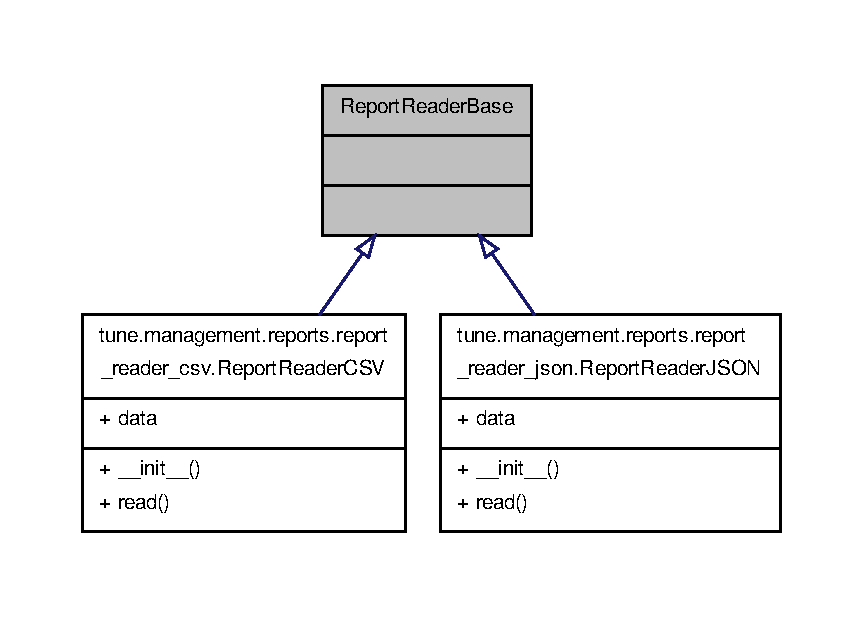
\includegraphics[width=350pt]{classReportReaderBase__inherit__graph}
\end{center}
\end{figure}


Collaboration diagram for Report\-Reader\-Base\-:
\nopagebreak
\begin{figure}[H]
\begin{center}
\leavevmode
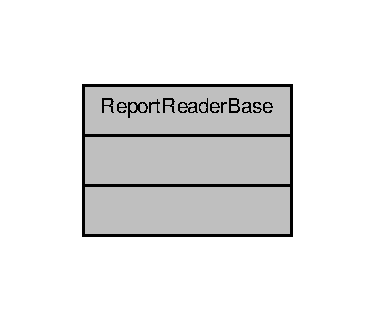
\includegraphics[width=180pt]{classReportReaderBase__coll__graph}
\end{center}
\end{figure}


The documentation for this class was generated from the following file\-:\begin{DoxyCompactItemize}
\item 
tune/management/reports/\hyperlink{report__reader__json_8py}{report\-\_\-reader\-\_\-json.\-py}\end{DoxyCompactItemize}

\hypertarget{classtune_1_1management_1_1reports_1_1report__reader__base_1_1ReportReaderBase}{\section{tune.\-management.\-reports.\-report\-\_\-reader\-\_\-base.\-Report\-Reader\-Base Class Reference}
\label{classtune_1_1management_1_1reports_1_1report__reader__base_1_1ReportReaderBase}\index{tune.\-management.\-reports.\-report\-\_\-reader\-\_\-base.\-Report\-Reader\-Base@{tune.\-management.\-reports.\-report\-\_\-reader\-\_\-base.\-Report\-Reader\-Base}}
}


Base Abstract class.  




Inheritance diagram for tune.\-management.\-reports.\-report\-\_\-reader\-\_\-base.\-Report\-Reader\-Base\-:
\nopagebreak
\begin{figure}[H]
\begin{center}
\leavevmode
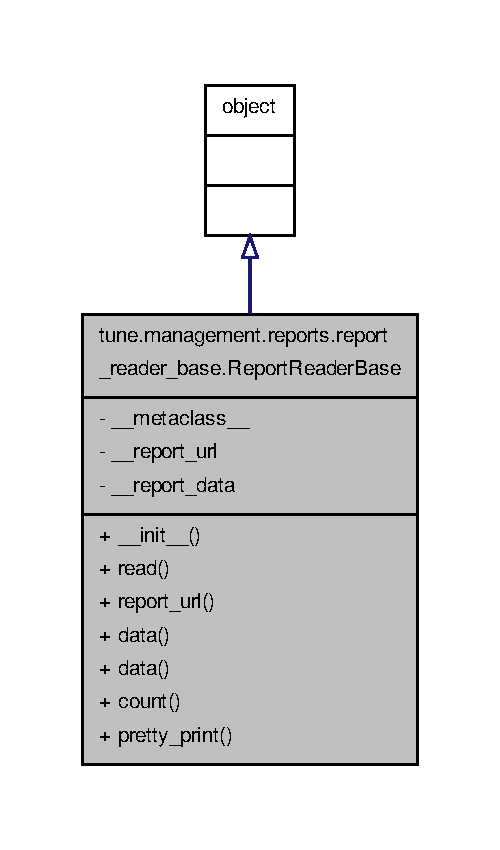
\includegraphics[width=240pt]{classtune_1_1management_1_1reports_1_1report__reader__base_1_1ReportReaderBase__inherit__graph}
\end{center}
\end{figure}


Collaboration diagram for tune.\-management.\-reports.\-report\-\_\-reader\-\_\-base.\-Report\-Reader\-Base\-:
\nopagebreak
\begin{figure}[H]
\begin{center}
\leavevmode
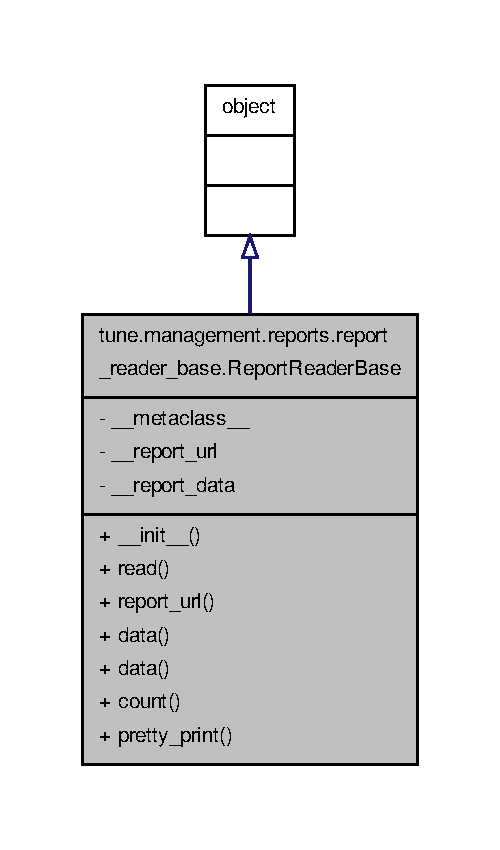
\includegraphics[width=240pt]{classtune_1_1management_1_1reports_1_1report__reader__base_1_1ReportReaderBase__coll__graph}
\end{center}
\end{figure}
\subsection*{Public Member Functions}
\begin{DoxyCompactItemize}
\item 
def \hyperlink{classtune_1_1management_1_1reports_1_1report__reader__base_1_1ReportReaderBase_a209c6b9ba1151084c53ef3767a75bcf3}{\-\_\-\-\_\-init\-\_\-\-\_\-}
\begin{DoxyCompactList}\small\item\em The constructor. \end{DoxyCompactList}\item 
def \hyperlink{classtune_1_1management_1_1reports_1_1report__reader__base_1_1ReportReaderBase_aa69b060ba23ee7403800be602c083a49}{read}
\begin{DoxyCompactList}\small\item\em Get property for Request Action Name. \end{DoxyCompactList}\item 
def \hyperlink{classtune_1_1management_1_1reports_1_1report__reader__base_1_1ReportReaderBase_ae6122bbe9996bc93ec9f9535ae568c77}{report\-\_\-url}
\begin{DoxyCompactList}\small\item\em R\-E\-P\-O\-R\-T\-\_\-\-U\-R\-L of completed report on S\-Q\-S. \end{DoxyCompactList}\item 
def \hyperlink{classtune_1_1management_1_1reports_1_1report__reader__base_1_1ReportReaderBase_a5c606aca915fa4590882722175756683}{data}
\begin{DoxyCompactList}\small\item\em Provide created reader populated with file data. \end{DoxyCompactList}\item 
def \hyperlink{classtune_1_1management_1_1reports_1_1report__reader__base_1_1ReportReaderBase_a5c606aca915fa4590882722175756683}{data}
\begin{DoxyCompactList}\small\item\em Provide data value. \end{DoxyCompactList}\item 
def \hyperlink{classtune_1_1management_1_1reports_1_1report__reader__base_1_1ReportReaderBase_a75cd9fbd6e625b7d7b4bf5bfce50ff3b}{count}
\begin{DoxyCompactList}\small\item\em Count number of row within gather file data. \end{DoxyCompactList}\item 
def \hyperlink{classtune_1_1management_1_1reports_1_1report__reader__base_1_1ReportReaderBase_ab6b5349638da5f23fc37a1b7d856f88b}{pretty\-\_\-print}
\begin{DoxyCompactList}\small\item\em Pretty print exported data. \end{DoxyCompactList}\end{DoxyCompactItemize}
\subsection*{Static Private Attributes}
\begin{DoxyCompactItemize}
\item 
\hyperlink{classtune_1_1management_1_1reports_1_1report__reader__base_1_1ReportReaderBase_a28f3b5212c0d73e7012eca3ab751de9a}{\-\_\-\-\_\-metaclass\-\_\-\-\_\-} = A\-B\-C\-Meta
\item 
\hyperlink{classtune_1_1management_1_1reports_1_1report__reader__base_1_1ReportReaderBase_a54ece2ab143966999222b2d9de8b9319}{\-\_\-\-\_\-report\-\_\-url} = None
\item 
\hyperlink{classtune_1_1management_1_1reports_1_1report__reader__base_1_1ReportReaderBase_a7f0df9aaf6dce143084db4849cbc1d12}{\-\_\-\-\_\-report\-\_\-data} = None
\end{DoxyCompactItemize}


\subsection{Detailed Description}
Base Abstract class. 



Definition at line 48 of file report\-\_\-reader\-\_\-base.\-py.



\subsection{Constructor \& Destructor Documentation}
\hypertarget{classtune_1_1management_1_1reports_1_1report__reader__base_1_1ReportReaderBase_a209c6b9ba1151084c53ef3767a75bcf3}{\index{tune\-::management\-::reports\-::report\-\_\-reader\-\_\-base\-::\-Report\-Reader\-Base@{tune\-::management\-::reports\-::report\-\_\-reader\-\_\-base\-::\-Report\-Reader\-Base}!\-\_\-\-\_\-init\-\_\-\-\_\-@{\-\_\-\-\_\-init\-\_\-\-\_\-}}
\index{\-\_\-\-\_\-init\-\_\-\-\_\-@{\-\_\-\-\_\-init\-\_\-\-\_\-}!tune::management::reports::report_reader_base::ReportReaderBase@{tune\-::management\-::reports\-::report\-\_\-reader\-\_\-base\-::\-Report\-Reader\-Base}}
\subsubsection[{\-\_\-\-\_\-init\-\_\-\-\_\-}]{\setlength{\rightskip}{0pt plus 5cm}def tune.\-management.\-reports.\-report\-\_\-reader\-\_\-base.\-Report\-Reader\-Base.\-\_\-\-\_\-init\-\_\-\-\_\- (
\begin{DoxyParamCaption}
\item[{}]{self, }
\item[{}]{report\-\_\-url}
\end{DoxyParamCaption}
)}}\label{classtune_1_1management_1_1reports_1_1report__reader__base_1_1ReportReaderBase_a209c6b9ba1151084c53ef3767a75bcf3}


The constructor. 


\begin{DoxyParams}{Parameters}
{\em string} & report\-\_\-url Download report U\-R\-L of requested report to be exported. \\
\hline
\end{DoxyParams}


Definition at line 58 of file report\-\_\-reader\-\_\-base.\-py.


\begin{DoxyCode}
58 
59     \textcolor{keyword}{def }\hyperlink{classtune_1_1management_1_1reports_1_1report__reader__base_1_1ReportReaderBase_a209c6b9ba1151084c53ef3767a75bcf3}{\_\_init\_\_}(self, report\_url):
60         self.\hyperlink{classtune_1_1management_1_1reports_1_1report__reader__base_1_1ReportReaderBase_a54ece2ab143966999222b2d9de8b9319}{\_\_report\_url} = report\_url
61         self.\hyperlink{classtune_1_1management_1_1reports_1_1report__reader__base_1_1ReportReaderBase_a7f0df9aaf6dce143084db4849cbc1d12}{\_\_report\_data} = \textcolor{keywordtype}{None}

\end{DoxyCode}


\subsection{Member Function Documentation}
\hypertarget{classtune_1_1management_1_1reports_1_1report__reader__base_1_1ReportReaderBase_a75cd9fbd6e625b7d7b4bf5bfce50ff3b}{\index{tune\-::management\-::reports\-::report\-\_\-reader\-\_\-base\-::\-Report\-Reader\-Base@{tune\-::management\-::reports\-::report\-\_\-reader\-\_\-base\-::\-Report\-Reader\-Base}!count@{count}}
\index{count@{count}!tune::management::reports::report_reader_base::ReportReaderBase@{tune\-::management\-::reports\-::report\-\_\-reader\-\_\-base\-::\-Report\-Reader\-Base}}
\subsubsection[{count}]{\setlength{\rightskip}{0pt plus 5cm}def tune.\-management.\-reports.\-report\-\_\-reader\-\_\-base.\-Report\-Reader\-Base.\-count (
\begin{DoxyParamCaption}
\item[{}]{self}
\end{DoxyParamCaption}
)}}\label{classtune_1_1management_1_1reports_1_1report__reader__base_1_1ReportReaderBase_a75cd9fbd6e625b7d7b4bf5bfce50ff3b}


Count number of row within gather file data. 



Definition at line 89 of file report\-\_\-reader\-\_\-base.\-py.


\begin{DoxyCode}
89 
90     \textcolor{keyword}{def }\hyperlink{classtune_1_1management_1_1reports_1_1report__reader__base_1_1ReportReaderBase_a75cd9fbd6e625b7d7b4bf5bfce50ff3b}{count}(self):
91         \textcolor{keywordflow}{return} len(self.\hyperlink{classtune_1_1management_1_1reports_1_1report__reader__base_1_1ReportReaderBase_a7f0df9aaf6dce143084db4849cbc1d12}{\_\_report\_data})

\end{DoxyCode}


Here is the caller graph for this function\-:
\nopagebreak
\begin{figure}[H]
\begin{center}
\leavevmode
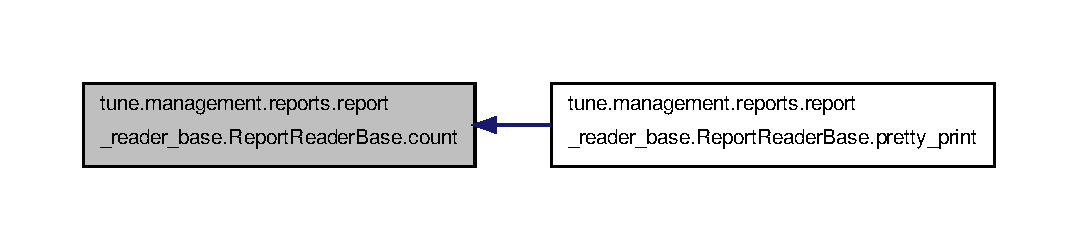
\includegraphics[width=350pt]{classtune_1_1management_1_1reports_1_1report__reader__base_1_1ReportReaderBase_a75cd9fbd6e625b7d7b4bf5bfce50ff3b_icgraph}
\end{center}
\end{figure}


\hypertarget{classtune_1_1management_1_1reports_1_1report__reader__base_1_1ReportReaderBase_a5c606aca915fa4590882722175756683}{\index{tune\-::management\-::reports\-::report\-\_\-reader\-\_\-base\-::\-Report\-Reader\-Base@{tune\-::management\-::reports\-::report\-\_\-reader\-\_\-base\-::\-Report\-Reader\-Base}!data@{data}}
\index{data@{data}!tune::management::reports::report_reader_base::ReportReaderBase@{tune\-::management\-::reports\-::report\-\_\-reader\-\_\-base\-::\-Report\-Reader\-Base}}
\subsubsection[{data}]{\setlength{\rightskip}{0pt plus 5cm}def tune.\-management.\-reports.\-report\-\_\-reader\-\_\-base.\-Report\-Reader\-Base.\-data (
\begin{DoxyParamCaption}
\item[{}]{self}
\end{DoxyParamCaption}
)}}\label{classtune_1_1management_1_1reports_1_1report__reader__base_1_1ReportReaderBase_a5c606aca915fa4590882722175756683}


Provide created reader populated with file data. 



Definition at line 77 of file report\-\_\-reader\-\_\-base.\-py.


\begin{DoxyCode}
77 
78     \textcolor{keyword}{def }\hyperlink{classtune_1_1management_1_1reports_1_1report__reader__base_1_1ReportReaderBase_a5c606aca915fa4590882722175756683}{data}(self):
79         \textcolor{keywordflow}{return} self.\hyperlink{classtune_1_1management_1_1reports_1_1report__reader__base_1_1ReportReaderBase_a7f0df9aaf6dce143084db4849cbc1d12}{\_\_report\_data}

\end{DoxyCode}


Here is the caller graph for this function\-:
\nopagebreak
\begin{figure}[H]
\begin{center}
\leavevmode
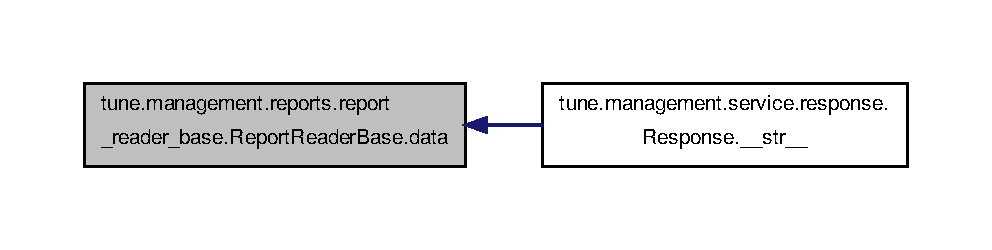
\includegraphics[width=350pt]{classtune_1_1management_1_1reports_1_1report__reader__base_1_1ReportReaderBase_a5c606aca915fa4590882722175756683_icgraph}
\end{center}
\end{figure}


\hypertarget{classtune_1_1management_1_1reports_1_1report__reader__base_1_1ReportReaderBase_a5c606aca915fa4590882722175756683}{\index{tune\-::management\-::reports\-::report\-\_\-reader\-\_\-base\-::\-Report\-Reader\-Base@{tune\-::management\-::reports\-::report\-\_\-reader\-\_\-base\-::\-Report\-Reader\-Base}!data@{data}}
\index{data@{data}!tune::management::reports::report_reader_base::ReportReaderBase@{tune\-::management\-::reports\-::report\-\_\-reader\-\_\-base\-::\-Report\-Reader\-Base}}
\subsubsection[{data}]{\setlength{\rightskip}{0pt plus 5cm}def tune.\-management.\-reports.\-report\-\_\-reader\-\_\-base.\-Report\-Reader\-Base.\-data (
\begin{DoxyParamCaption}
\item[{}]{self, }
\item[{}]{value}
\end{DoxyParamCaption}
)}}\label{classtune_1_1management_1_1reports_1_1report__reader__base_1_1ReportReaderBase_a5c606aca915fa4590882722175756683}


Provide data value. 



Definition at line 83 of file report\-\_\-reader\-\_\-base.\-py.


\begin{DoxyCode}
83 
84     \textcolor{keyword}{def }\hyperlink{classtune_1_1management_1_1reports_1_1report__reader__base_1_1ReportReaderBase_a5c606aca915fa4590882722175756683}{data}(self, value):
85         self.\hyperlink{classtune_1_1management_1_1reports_1_1report__reader__base_1_1ReportReaderBase_a7f0df9aaf6dce143084db4849cbc1d12}{\_\_report\_data} = value

\end{DoxyCode}


Here is the call graph for this function\-:
\nopagebreak
\begin{figure}[H]
\begin{center}
\leavevmode
\includegraphics[width=264pt]{classtune_1_1management_1_1reports_1_1report__reader__base_1_1ReportReaderBase_a5c606aca915fa4590882722175756683_cgraph}
\end{center}
\end{figure}




Here is the caller graph for this function\-:
\nopagebreak
\begin{figure}[H]
\begin{center}
\leavevmode
\includegraphics[width=350pt]{classtune_1_1management_1_1reports_1_1report__reader__base_1_1ReportReaderBase_a5c606aca915fa4590882722175756683_icgraph}
\end{center}
\end{figure}


\hypertarget{classtune_1_1management_1_1reports_1_1report__reader__base_1_1ReportReaderBase_ab6b5349638da5f23fc37a1b7d856f88b}{\index{tune\-::management\-::reports\-::report\-\_\-reader\-\_\-base\-::\-Report\-Reader\-Base@{tune\-::management\-::reports\-::report\-\_\-reader\-\_\-base\-::\-Report\-Reader\-Base}!pretty\-\_\-print@{pretty\-\_\-print}}
\index{pretty\-\_\-print@{pretty\-\_\-print}!tune::management::reports::report_reader_base::ReportReaderBase@{tune\-::management\-::reports\-::report\-\_\-reader\-\_\-base\-::\-Report\-Reader\-Base}}
\subsubsection[{pretty\-\_\-print}]{\setlength{\rightskip}{0pt plus 5cm}def tune.\-management.\-reports.\-report\-\_\-reader\-\_\-base.\-Report\-Reader\-Base.\-pretty\-\_\-print (
\begin{DoxyParamCaption}
\item[{}]{self, }
\item[{}]{limit = {\ttfamily 0}}
\end{DoxyParamCaption}
)}}\label{classtune_1_1management_1_1reports_1_1report__reader__base_1_1ReportReaderBase_ab6b5349638da5f23fc37a1b7d856f88b}


Pretty print exported data. 



Definition at line 94 of file report\-\_\-reader\-\_\-base.\-py.


\begin{DoxyCode}
94 
95     \textcolor{keyword}{def }\hyperlink{classtune_1_1management_1_1reports_1_1report__reader__base_1_1ReportReaderBase_ab6b5349638da5f23fc37a1b7d856f88b}{pretty\_print}(self, limit=0):
96         print(\textcolor{stringliteral}{"Report REPORT\_URL: \{\}"}.format(self.\hyperlink{classtune_1_1management_1_1reports_1_1report__reader__base_1_1ReportReaderBase_ae6122bbe9996bc93ec9f9535ae568c77}{report\_url}))
97         print(\textcolor{stringliteral}{"Report total row count: \{\}"}.format(self.\hyperlink{classtune_1_1management_1_1reports_1_1report__reader__base_1_1ReportReaderBase_a75cd9fbd6e625b7d7b4bf5bfce50ff3b}{count}))
98         \textcolor{keywordflow}{if} self.\hyperlink{classtune_1_1management_1_1reports_1_1report__reader__base_1_1ReportReaderBase_a75cd9fbd6e625b7d7b4bf5bfce50ff3b}{count} > 0:
99             print(\textcolor{stringliteral}{"------------------"})
100             rows = list(self.\hyperlink{classtune_1_1management_1_1reports_1_1report__reader__base_1_1ReportReaderBase_a5c606aca915fa4590882722175756683}{data})
101             \textcolor{keywordflow}{for} i, row \textcolor{keywordflow}{in} enumerate(rows):
102                 print(\textcolor{stringliteral}{"\{\}. \{\}"}.format(i+1, str(row)))
103                 \textcolor{keywordflow}{if} (limit > 0) \textcolor{keywordflow}{and} (i > limit):
104                     \textcolor{keywordflow}{break}
105             print(\textcolor{stringliteral}{"------------------"})
\end{DoxyCode}


Here is the call graph for this function\-:
\nopagebreak
\begin{figure}[H]
\begin{center}
\leavevmode
\includegraphics[width=350pt]{classtune_1_1management_1_1reports_1_1report__reader__base_1_1ReportReaderBase_ab6b5349638da5f23fc37a1b7d856f88b_cgraph}
\end{center}
\end{figure}


\hypertarget{classtune_1_1management_1_1reports_1_1report__reader__base_1_1ReportReaderBase_aa69b060ba23ee7403800be602c083a49}{\index{tune\-::management\-::reports\-::report\-\_\-reader\-\_\-base\-::\-Report\-Reader\-Base@{tune\-::management\-::reports\-::report\-\_\-reader\-\_\-base\-::\-Report\-Reader\-Base}!read@{read}}
\index{read@{read}!tune::management::reports::report_reader_base::ReportReaderBase@{tune\-::management\-::reports\-::report\-\_\-reader\-\_\-base\-::\-Report\-Reader\-Base}}
\subsubsection[{read}]{\setlength{\rightskip}{0pt plus 5cm}def tune.\-management.\-reports.\-report\-\_\-reader\-\_\-base.\-Report\-Reader\-Base.\-read (
\begin{DoxyParamCaption}
\item[{}]{self}
\end{DoxyParamCaption}
)}}\label{classtune_1_1management_1_1reports_1_1report__reader__base_1_1ReportReaderBase_aa69b060ba23ee7403800be602c083a49}


Get property for Request Action Name. 



Definition at line 65 of file report\-\_\-reader\-\_\-base.\-py.


\begin{DoxyCode}
65 
66     \textcolor{keyword}{def }\hyperlink{classtune_1_1management_1_1reports_1_1report__reader__base_1_1ReportReaderBase_aa69b060ba23ee7403800be602c083a49}{read}(self):
67         \textcolor{keywordflow}{return}

\end{DoxyCode}
\hypertarget{classtune_1_1management_1_1reports_1_1report__reader__base_1_1ReportReaderBase_ae6122bbe9996bc93ec9f9535ae568c77}{\index{tune\-::management\-::reports\-::report\-\_\-reader\-\_\-base\-::\-Report\-Reader\-Base@{tune\-::management\-::reports\-::report\-\_\-reader\-\_\-base\-::\-Report\-Reader\-Base}!report\-\_\-url@{report\-\_\-url}}
\index{report\-\_\-url@{report\-\_\-url}!tune::management::reports::report_reader_base::ReportReaderBase@{tune\-::management\-::reports\-::report\-\_\-reader\-\_\-base\-::\-Report\-Reader\-Base}}
\subsubsection[{report\-\_\-url}]{\setlength{\rightskip}{0pt plus 5cm}def tune.\-management.\-reports.\-report\-\_\-reader\-\_\-base.\-Report\-Reader\-Base.\-report\-\_\-url (
\begin{DoxyParamCaption}
\item[{}]{self}
\end{DoxyParamCaption}
)}}\label{classtune_1_1management_1_1reports_1_1report__reader__base_1_1ReportReaderBase_ae6122bbe9996bc93ec9f9535ae568c77}


R\-E\-P\-O\-R\-T\-\_\-\-U\-R\-L of completed report on S\-Q\-S. 



Definition at line 71 of file report\-\_\-reader\-\_\-base.\-py.


\begin{DoxyCode}
71 
72     \textcolor{keyword}{def }\hyperlink{classtune_1_1management_1_1reports_1_1report__reader__base_1_1ReportReaderBase_ae6122bbe9996bc93ec9f9535ae568c77}{report\_url}(self):
73         \textcolor{keywordflow}{return} self.\hyperlink{classtune_1_1management_1_1reports_1_1report__reader__base_1_1ReportReaderBase_a54ece2ab143966999222b2d9de8b9319}{\_\_report\_url}

\end{DoxyCode}


Here is the caller graph for this function\-:
\nopagebreak
\begin{figure}[H]
\begin{center}
\leavevmode
\includegraphics[width=350pt]{classtune_1_1management_1_1reports_1_1report__reader__base_1_1ReportReaderBase_ae6122bbe9996bc93ec9f9535ae568c77_icgraph}
\end{center}
\end{figure}




\subsection{Member Data Documentation}
\hypertarget{classtune_1_1management_1_1reports_1_1report__reader__base_1_1ReportReaderBase_a28f3b5212c0d73e7012eca3ab751de9a}{\index{tune\-::management\-::reports\-::report\-\_\-reader\-\_\-base\-::\-Report\-Reader\-Base@{tune\-::management\-::reports\-::report\-\_\-reader\-\_\-base\-::\-Report\-Reader\-Base}!\-\_\-\-\_\-metaclass\-\_\-\-\_\-@{\-\_\-\-\_\-metaclass\-\_\-\-\_\-}}
\index{\-\_\-\-\_\-metaclass\-\_\-\-\_\-@{\-\_\-\-\_\-metaclass\-\_\-\-\_\-}!tune::management::reports::report_reader_base::ReportReaderBase@{tune\-::management\-::reports\-::report\-\_\-reader\-\_\-base\-::\-Report\-Reader\-Base}}
\subsubsection[{\-\_\-\-\_\-metaclass\-\_\-\-\_\-}]{\setlength{\rightskip}{0pt plus 5cm}tune.\-management.\-reports.\-report\-\_\-reader\-\_\-base.\-Report\-Reader\-Base.\-\_\-\-\_\-metaclass\-\_\-\-\_\- = A\-B\-C\-Meta\hspace{0.3cm}{\ttfamily [static]}, {\ttfamily [private]}}}\label{classtune_1_1management_1_1reports_1_1report__reader__base_1_1ReportReaderBase_a28f3b5212c0d73e7012eca3ab751de9a}


Definition at line 50 of file report\-\_\-reader\-\_\-base.\-py.

\hypertarget{classtune_1_1management_1_1reports_1_1report__reader__base_1_1ReportReaderBase_a7f0df9aaf6dce143084db4849cbc1d12}{\index{tune\-::management\-::reports\-::report\-\_\-reader\-\_\-base\-::\-Report\-Reader\-Base@{tune\-::management\-::reports\-::report\-\_\-reader\-\_\-base\-::\-Report\-Reader\-Base}!\-\_\-\-\_\-report\-\_\-data@{\-\_\-\-\_\-report\-\_\-data}}
\index{\-\_\-\-\_\-report\-\_\-data@{\-\_\-\-\_\-report\-\_\-data}!tune::management::reports::report_reader_base::ReportReaderBase@{tune\-::management\-::reports\-::report\-\_\-reader\-\_\-base\-::\-Report\-Reader\-Base}}
\subsubsection[{\-\_\-\-\_\-report\-\_\-data}]{\setlength{\rightskip}{0pt plus 5cm}tune.\-management.\-reports.\-report\-\_\-reader\-\_\-base.\-Report\-Reader\-Base.\-\_\-\-\_\-report\-\_\-data = None\hspace{0.3cm}{\ttfamily [static]}, {\ttfamily [private]}}}\label{classtune_1_1management_1_1reports_1_1report__reader__base_1_1ReportReaderBase_a7f0df9aaf6dce143084db4849cbc1d12}


Definition at line 53 of file report\-\_\-reader\-\_\-base.\-py.

\hypertarget{classtune_1_1management_1_1reports_1_1report__reader__base_1_1ReportReaderBase_a54ece2ab143966999222b2d9de8b9319}{\index{tune\-::management\-::reports\-::report\-\_\-reader\-\_\-base\-::\-Report\-Reader\-Base@{tune\-::management\-::reports\-::report\-\_\-reader\-\_\-base\-::\-Report\-Reader\-Base}!\-\_\-\-\_\-report\-\_\-url@{\-\_\-\-\_\-report\-\_\-url}}
\index{\-\_\-\-\_\-report\-\_\-url@{\-\_\-\-\_\-report\-\_\-url}!tune::management::reports::report_reader_base::ReportReaderBase@{tune\-::management\-::reports\-::report\-\_\-reader\-\_\-base\-::\-Report\-Reader\-Base}}
\subsubsection[{\-\_\-\-\_\-report\-\_\-url}]{\setlength{\rightskip}{0pt plus 5cm}tune.\-management.\-reports.\-report\-\_\-reader\-\_\-base.\-Report\-Reader\-Base.\-\_\-\-\_\-report\-\_\-url = None\hspace{0.3cm}{\ttfamily [static]}, {\ttfamily [private]}}}\label{classtune_1_1management_1_1reports_1_1report__reader__base_1_1ReportReaderBase_a54ece2ab143966999222b2d9de8b9319}


Definition at line 52 of file report\-\_\-reader\-\_\-base.\-py.



The documentation for this class was generated from the following file\-:\begin{DoxyCompactItemize}
\item 
tune/management/reports/\hyperlink{report__reader__base_8py}{report\-\_\-reader\-\_\-base.\-py}\end{DoxyCompactItemize}

\hypertarget{classtune_1_1management_1_1reports_1_1report__reader__csv_1_1ReportReaderCSV}{\section{tune.\-management.\-reports.\-report\-\_\-reader\-\_\-csv.\-Report\-Reader\-C\-S\-V Class Reference}
\label{classtune_1_1management_1_1reports_1_1report__reader__csv_1_1ReportReaderCSV}\index{tune.\-management.\-reports.\-report\-\_\-reader\-\_\-csv.\-Report\-Reader\-C\-S\-V@{tune.\-management.\-reports.\-report\-\_\-reader\-\_\-csv.\-Report\-Reader\-C\-S\-V}}
}


Helper class for reading reading remote C\-S\-V file.  




Inheritance diagram for tune.\-management.\-reports.\-report\-\_\-reader\-\_\-csv.\-Report\-Reader\-C\-S\-V\-:
\nopagebreak
\begin{figure}[H]
\begin{center}
\leavevmode
\includegraphics[width=234pt]{classtune_1_1management_1_1reports_1_1report__reader__csv_1_1ReportReaderCSV__inherit__graph}
\end{center}
\end{figure}


Collaboration diagram for tune.\-management.\-reports.\-report\-\_\-reader\-\_\-csv.\-Report\-Reader\-C\-S\-V\-:
\nopagebreak
\begin{figure}[H]
\begin{center}
\leavevmode
\includegraphics[width=234pt]{classtune_1_1management_1_1reports_1_1report__reader__csv_1_1ReportReaderCSV__coll__graph}
\end{center}
\end{figure}
\subsection*{Public Member Functions}
\begin{DoxyCompactItemize}
\item 
def \hyperlink{classtune_1_1management_1_1reports_1_1report__reader__csv_1_1ReportReaderCSV_a418f8a33369c1269d59406d70c4d5562}{\-\_\-\-\_\-init\-\_\-\-\_\-}
\begin{DoxyCompactList}\small\item\em The constructor. \end{DoxyCompactList}\item 
def \hyperlink{classtune_1_1management_1_1reports_1_1report__reader__csv_1_1ReportReaderCSV_a761840bd958d0c771e9638a637bcfd55}{read}
\begin{DoxyCompactList}\small\item\em Using provided report download U\-R\-L, extract C\-S\-V contents. \end{DoxyCompactList}\end{DoxyCompactItemize}
\subsection*{Public Attributes}
\begin{DoxyCompactItemize}
\item 
\hyperlink{classtune_1_1management_1_1reports_1_1report__reader__csv_1_1ReportReaderCSV_a54edf30f0b976974d271d655393f90d8}{data}
\end{DoxyCompactItemize}


\subsection{Detailed Description}
Helper class for reading reading remote C\-S\-V file. 

Helper class for reading reading remote C\-S\-V file 

Definition at line 60 of file report\-\_\-reader\-\_\-csv.\-py.



\subsection{Constructor \& Destructor Documentation}
\hypertarget{classtune_1_1management_1_1reports_1_1report__reader__csv_1_1ReportReaderCSV_a418f8a33369c1269d59406d70c4d5562}{\index{tune\-::management\-::reports\-::report\-\_\-reader\-\_\-csv\-::\-Report\-Reader\-C\-S\-V@{tune\-::management\-::reports\-::report\-\_\-reader\-\_\-csv\-::\-Report\-Reader\-C\-S\-V}!\-\_\-\-\_\-init\-\_\-\-\_\-@{\-\_\-\-\_\-init\-\_\-\-\_\-}}
\index{\-\_\-\-\_\-init\-\_\-\-\_\-@{\-\_\-\-\_\-init\-\_\-\-\_\-}!tune::management::reports::report_reader_csv::ReportReaderCSV@{tune\-::management\-::reports\-::report\-\_\-reader\-\_\-csv\-::\-Report\-Reader\-C\-S\-V}}
\subsubsection[{\-\_\-\-\_\-init\-\_\-\-\_\-}]{\setlength{\rightskip}{0pt plus 5cm}def tune.\-management.\-reports.\-report\-\_\-reader\-\_\-csv.\-Report\-Reader\-C\-S\-V.\-\_\-\-\_\-init\-\_\-\-\_\- (
\begin{DoxyParamCaption}
\item[{}]{self, }
\item[{}]{report\-\_\-url}
\end{DoxyParamCaption}
)}}\label{classtune_1_1management_1_1reports_1_1report__reader__csv_1_1ReportReaderCSV_a418f8a33369c1269d59406d70c4d5562}


The constructor. 


\begin{DoxyParams}{Parameters}
{\em string} & report\-\_\-url Download report U\-R\-L of requested report to be exported. \\
\hline
\end{DoxyParams}


Definition at line 65 of file report\-\_\-reader\-\_\-csv.\-py.


\begin{DoxyCode}
65 
66     \textcolor{keyword}{def }\hyperlink{classtune_1_1management_1_1reports_1_1report__reader__csv_1_1ReportReaderCSV_a418f8a33369c1269d59406d70c4d5562}{\_\_init\_\_}(self, report\_url):
67         ReportReaderBase.\_\_init\_\_(self, report\_url)

\end{DoxyCode}


\subsection{Member Function Documentation}
\hypertarget{classtune_1_1management_1_1reports_1_1report__reader__csv_1_1ReportReaderCSV_a761840bd958d0c771e9638a637bcfd55}{\index{tune\-::management\-::reports\-::report\-\_\-reader\-\_\-csv\-::\-Report\-Reader\-C\-S\-V@{tune\-::management\-::reports\-::report\-\_\-reader\-\_\-csv\-::\-Report\-Reader\-C\-S\-V}!read@{read}}
\index{read@{read}!tune::management::reports::report_reader_csv::ReportReaderCSV@{tune\-::management\-::reports\-::report\-\_\-reader\-\_\-csv\-::\-Report\-Reader\-C\-S\-V}}
\subsubsection[{read}]{\setlength{\rightskip}{0pt plus 5cm}def tune.\-management.\-reports.\-report\-\_\-reader\-\_\-csv.\-Report\-Reader\-C\-S\-V.\-read (
\begin{DoxyParamCaption}
\item[{}]{self}
\end{DoxyParamCaption}
)}}\label{classtune_1_1management_1_1reports_1_1report__reader__csv_1_1ReportReaderCSV_a761840bd958d0c771e9638a637bcfd55}


Using provided report download U\-R\-L, extract C\-S\-V contents. 

Read C\-S\-V data provided remote path report\-\_\-url. 

Definition at line 72 of file report\-\_\-reader\-\_\-csv.\-py.


\begin{DoxyCode}
72 
73     \textcolor{keyword}{def }\hyperlink{classtune_1_1management_1_1reports_1_1report__reader__csv_1_1ReportReaderCSV_a761840bd958d0c771e9638a637bcfd55}{read}(self):
74 
75         self.\hyperlink{classtune_1_1management_1_1reports_1_1report__reader__csv_1_1ReportReaderCSV_a54edf30f0b976974d271d655393f90d8}{data} = []
76         report\_reader = \textcolor{keywordtype}{None}
77         \textcolor{keywordflow}{try}:
78             report\_stream = urllib.request.urlopen(self.report\_url)
79             report\_reader = csv.reader(codecs.iterdecode(report\_stream, \textcolor{stringliteral}{'utf-8'}))
80         \textcolor{keywordflow}{except} urllib.error.URLError \textcolor{keyword}{as} ex:
81             \textcolor{keywordflow}{raise} TuneServiceException(\textcolor{stringliteral}{"URLError: \{\}"}.format(str(ex)), ex)
82         \textcolor{keywordflow}{except} urllib.error.HTTPError \textcolor{keyword}{as} ex:
83             \textcolor{keywordflow}{raise} TuneServiceException(\textcolor{stringliteral}{"HTTPError: \{\}"}.format(str(ex)), ex)
84         \textcolor{keywordflow}{except} Exception \textcolor{keyword}{as} ex:
85             \textcolor{keywordflow}{raise} TuneSdkException(
86                 \textcolor{stringliteral}{"Unexpected: \{\}: \{\}"}.format(ex.\_\_class\_\_.\_\_name\_\_, str(ex)),
87                 ex
88             )
89 
90         \textcolor{keywordflow}{if} \textcolor{keywordflow}{not} report\_reader:
91             \textcolor{keywordflow}{raise} TuneSdkException(\textcolor{stringliteral}{"CSV Reader not provided."})
92 
93         \textcolor{keywordflow}{for} row \textcolor{keywordflow}{in} report\_reader:
94             self.data.append(row)
\end{DoxyCode}


\subsection{Member Data Documentation}
\hypertarget{classtune_1_1management_1_1reports_1_1report__reader__csv_1_1ReportReaderCSV_a54edf30f0b976974d271d655393f90d8}{\index{tune\-::management\-::reports\-::report\-\_\-reader\-\_\-csv\-::\-Report\-Reader\-C\-S\-V@{tune\-::management\-::reports\-::report\-\_\-reader\-\_\-csv\-::\-Report\-Reader\-C\-S\-V}!data@{data}}
\index{data@{data}!tune::management::reports::report_reader_csv::ReportReaderCSV@{tune\-::management\-::reports\-::report\-\_\-reader\-\_\-csv\-::\-Report\-Reader\-C\-S\-V}}
\subsubsection[{data}]{\setlength{\rightskip}{0pt plus 5cm}tune.\-management.\-reports.\-report\-\_\-reader\-\_\-csv.\-Report\-Reader\-C\-S\-V.\-data}}\label{classtune_1_1management_1_1reports_1_1report__reader__csv_1_1ReportReaderCSV_a54edf30f0b976974d271d655393f90d8}


Definition at line 74 of file report\-\_\-reader\-\_\-csv.\-py.



The documentation for this class was generated from the following file\-:\begin{DoxyCompactItemize}
\item 
tune/management/reports/\hyperlink{report__reader__csv_8py}{report\-\_\-reader\-\_\-csv.\-py}\end{DoxyCompactItemize}

\hypertarget{classtune_1_1management_1_1reports_1_1report__reader__json_1_1ReportReaderJSON}{\section{tune.\-management.\-reports.\-report\-\_\-reader\-\_\-json.\-Report\-Reader\-J\-S\-O\-N Class Reference}
\label{classtune_1_1management_1_1reports_1_1report__reader__json_1_1ReportReaderJSON}\index{tune.\-management.\-reports.\-report\-\_\-reader\-\_\-json.\-Report\-Reader\-J\-S\-O\-N@{tune.\-management.\-reports.\-report\-\_\-reader\-\_\-json.\-Report\-Reader\-J\-S\-O\-N}}
}


Helper class for reading reading remote J\-S\-O\-N file.  




Inheritance diagram for tune.\-management.\-reports.\-report\-\_\-reader\-\_\-json.\-Report\-Reader\-J\-S\-O\-N\-:
\nopagebreak
\begin{figure}[H]
\begin{center}
\leavevmode
\includegraphics[width=242pt]{classtune_1_1management_1_1reports_1_1report__reader__json_1_1ReportReaderJSON__inherit__graph}
\end{center}
\end{figure}


Collaboration diagram for tune.\-management.\-reports.\-report\-\_\-reader\-\_\-json.\-Report\-Reader\-J\-S\-O\-N\-:
\nopagebreak
\begin{figure}[H]
\begin{center}
\leavevmode
\includegraphics[width=242pt]{classtune_1_1management_1_1reports_1_1report__reader__json_1_1ReportReaderJSON__coll__graph}
\end{center}
\end{figure}
\subsection*{Public Member Functions}
\begin{DoxyCompactItemize}
\item 
def \hyperlink{classtune_1_1management_1_1reports_1_1report__reader__json_1_1ReportReaderJSON_aa828e0e4a41834a6a678224676df232c}{\-\_\-\-\_\-init\-\_\-\-\_\-}
\begin{DoxyCompactList}\small\item\em The constructor. \end{DoxyCompactList}\item 
def \hyperlink{classtune_1_1management_1_1reports_1_1report__reader__json_1_1ReportReaderJSON_a9690c4e4ce8f0e9ab5e827eafbc9ccdf}{read}
\begin{DoxyCompactList}\small\item\em Using provided report download U\-R\-L, extract J\-S\-O\-N contents. \end{DoxyCompactList}\end{DoxyCompactItemize}
\subsection*{Public Attributes}
\begin{DoxyCompactItemize}
\item 
\hyperlink{classtune_1_1management_1_1reports_1_1report__reader__json_1_1ReportReaderJSON_a75b908b0ea9e8a3b405eab59294199a4}{data}
\end{DoxyCompactItemize}


\subsection{Detailed Description}
Helper class for reading reading remote J\-S\-O\-N file. 

Definition at line 58 of file report\-\_\-reader\-\_\-json.\-py.



\subsection{Constructor \& Destructor Documentation}
\hypertarget{classtune_1_1management_1_1reports_1_1report__reader__json_1_1ReportReaderJSON_aa828e0e4a41834a6a678224676df232c}{\index{tune\-::management\-::reports\-::report\-\_\-reader\-\_\-json\-::\-Report\-Reader\-J\-S\-O\-N@{tune\-::management\-::reports\-::report\-\_\-reader\-\_\-json\-::\-Report\-Reader\-J\-S\-O\-N}!\-\_\-\-\_\-init\-\_\-\-\_\-@{\-\_\-\-\_\-init\-\_\-\-\_\-}}
\index{\-\_\-\-\_\-init\-\_\-\-\_\-@{\-\_\-\-\_\-init\-\_\-\-\_\-}!tune::management::reports::report_reader_json::ReportReaderJSON@{tune\-::management\-::reports\-::report\-\_\-reader\-\_\-json\-::\-Report\-Reader\-J\-S\-O\-N}}
\subsubsection[{\-\_\-\-\_\-init\-\_\-\-\_\-}]{\setlength{\rightskip}{0pt plus 5cm}def tune.\-management.\-reports.\-report\-\_\-reader\-\_\-json.\-Report\-Reader\-J\-S\-O\-N.\-\_\-\-\_\-init\-\_\-\-\_\- (
\begin{DoxyParamCaption}
\item[{}]{self, }
\item[{}]{report\-\_\-url}
\end{DoxyParamCaption}
)}}\label{classtune_1_1management_1_1reports_1_1report__reader__json_1_1ReportReaderJSON_aa828e0e4a41834a6a678224676df232c}


The constructor. 


\begin{DoxyParams}{Parameters}
{\em string} & report\-\_\-url Download report U\-R\-L of requested report to be exported. \\
\hline
\end{DoxyParams}


Definition at line 63 of file report\-\_\-reader\-\_\-json.\-py.


\begin{DoxyCode}
63 
64     \textcolor{keyword}{def }\hyperlink{classtune_1_1management_1_1reports_1_1report__reader__json_1_1ReportReaderJSON_aa828e0e4a41834a6a678224676df232c}{\_\_init\_\_}(self, report\_url):
65         ReportReaderBase.\_\_init\_\_(self, report\_url)

\end{DoxyCode}


\subsection{Member Function Documentation}
\hypertarget{classtune_1_1management_1_1reports_1_1report__reader__json_1_1ReportReaderJSON_a9690c4e4ce8f0e9ab5e827eafbc9ccdf}{\index{tune\-::management\-::reports\-::report\-\_\-reader\-\_\-json\-::\-Report\-Reader\-J\-S\-O\-N@{tune\-::management\-::reports\-::report\-\_\-reader\-\_\-json\-::\-Report\-Reader\-J\-S\-O\-N}!read@{read}}
\index{read@{read}!tune::management::reports::report_reader_json::ReportReaderJSON@{tune\-::management\-::reports\-::report\-\_\-reader\-\_\-json\-::\-Report\-Reader\-J\-S\-O\-N}}
\subsubsection[{read}]{\setlength{\rightskip}{0pt plus 5cm}def tune.\-management.\-reports.\-report\-\_\-reader\-\_\-json.\-Report\-Reader\-J\-S\-O\-N.\-read (
\begin{DoxyParamCaption}
\item[{}]{self}
\end{DoxyParamCaption}
)}}\label{classtune_1_1management_1_1reports_1_1report__reader__json_1_1ReportReaderJSON_a9690c4e4ce8f0e9ab5e827eafbc9ccdf}


Using provided report download U\-R\-L, extract J\-S\-O\-N contents. 

Read J\-S\-O\-N data provided remote path report\-\_\-url. 

Definition at line 70 of file report\-\_\-reader\-\_\-json.\-py.


\begin{DoxyCode}
70 
71     \textcolor{keyword}{def }\hyperlink{classtune_1_1management_1_1reports_1_1report__reader__json_1_1ReportReaderJSON_a9690c4e4ce8f0e9ab5e827eafbc9ccdf}{read}(self):
72         self.\hyperlink{classtune_1_1management_1_1reports_1_1report__reader__json_1_1ReportReaderJSON_a75b908b0ea9e8a3b405eab59294199a4}{data} = \textcolor{keywordtype}{None}
73         \textcolor{keywordflow}{try}:
74             report\_stream = urllib.request.urlopen(self.report\_url)
75             report\_content = report\_stream.read()
76             report\_utf8\_str = report\_content.decode(\textcolor{stringliteral}{"utf8"})
77             self.\hyperlink{classtune_1_1management_1_1reports_1_1report__reader__json_1_1ReportReaderJSON_a75b908b0ea9e8a3b405eab59294199a4}{data} = json.loads(report\_utf8\_str)
78         \textcolor{keywordflow}{except} urllib.error.URLError \textcolor{keyword}{as} ex:
79             \textcolor{keywordflow}{raise} TuneServiceException(\textcolor{stringliteral}{"URLError: \{\}"}.format(str(ex)), ex)
80         \textcolor{keywordflow}{except} urllib.error.HTTPError \textcolor{keyword}{as} ex:
81             \textcolor{keywordflow}{raise} TuneServiceException(\textcolor{stringliteral}{"HTTPError: \{\}"}.format(str(ex)), ex)
82         \textcolor{keywordflow}{except} Exception \textcolor{keyword}{as} ex:
83             \textcolor{keywordflow}{raise} TuneSdkException(
84                 \textcolor{stringliteral}{"Unexpected: \{\}: \{\}"}.format(ex.\_\_class\_\_.\_\_name\_\_, str(ex)), ex
85             )
\end{DoxyCode}


\subsection{Member Data Documentation}
\hypertarget{classtune_1_1management_1_1reports_1_1report__reader__json_1_1ReportReaderJSON_a75b908b0ea9e8a3b405eab59294199a4}{\index{tune\-::management\-::reports\-::report\-\_\-reader\-\_\-json\-::\-Report\-Reader\-J\-S\-O\-N@{tune\-::management\-::reports\-::report\-\_\-reader\-\_\-json\-::\-Report\-Reader\-J\-S\-O\-N}!data@{data}}
\index{data@{data}!tune::management::reports::report_reader_json::ReportReaderJSON@{tune\-::management\-::reports\-::report\-\_\-reader\-\_\-json\-::\-Report\-Reader\-J\-S\-O\-N}}
\subsubsection[{data}]{\setlength{\rightskip}{0pt plus 5cm}tune.\-management.\-reports.\-report\-\_\-reader\-\_\-json.\-Report\-Reader\-J\-S\-O\-N.\-data}}\label{classtune_1_1management_1_1reports_1_1report__reader__json_1_1ReportReaderJSON_a75b908b0ea9e8a3b405eab59294199a4}


Definition at line 71 of file report\-\_\-reader\-\_\-json.\-py.



The documentation for this class was generated from the following file\-:\begin{DoxyCompactItemize}
\item 
tune/management/reports/\hyperlink{report__reader__json_8py}{report\-\_\-reader\-\_\-json.\-py}\end{DoxyCompactItemize}

\hypertarget{classReportsActualsBase}{\section{Reports\-Actuals\-Base Class Reference}
\label{classReportsActualsBase}\index{Reports\-Actuals\-Base@{Reports\-Actuals\-Base}}
}


Inheritance diagram for Reports\-Actuals\-Base\-:
\nopagebreak
\begin{figure}[H]
\begin{center}
\leavevmode
\includegraphics[width=262pt]{classReportsActualsBase__inherit__graph}
\end{center}
\end{figure}


Collaboration diagram for Reports\-Actuals\-Base\-:
\nopagebreak
\begin{figure}[H]
\begin{center}
\leavevmode
\includegraphics[width=186pt]{classReportsActualsBase__coll__graph}
\end{center}
\end{figure}


The documentation for this class was generated from the following file\-:\begin{DoxyCompactItemize}
\item 
tune/management/api/advertiser/stats/\hyperlink{management_2api_2advertiser_2stats_2____init_____8py}{\-\_\-\-\_\-init\-\_\-\-\_\-.\-py}\end{DoxyCompactItemize}

\hypertarget{classtune_1_1management_1_1reports_1_1reports__actuals__base_1_1ReportsActualsBase}{\section{tune.\-management.\-reports.\-reports\-\_\-actuals\-\_\-base.\-Reports\-Actuals\-Base Class Reference}
\label{classtune_1_1management_1_1reports_1_1reports__actuals__base_1_1ReportsActualsBase}\index{tune.\-management.\-reports.\-reports\-\_\-actuals\-\_\-base.\-Reports\-Actuals\-Base@{tune.\-management.\-reports.\-reports\-\_\-actuals\-\_\-base.\-Reports\-Actuals\-Base}}
}


Base class intended for gathering from Advertiser Stats actuals.  




Inheritance diagram for tune.\-management.\-reports.\-reports\-\_\-actuals\-\_\-base.\-Reports\-Actuals\-Base\-:
\nopagebreak
\begin{figure}[H]
\begin{center}
\leavevmode
\includegraphics[width=252pt]{classtune_1_1management_1_1reports_1_1reports__actuals__base_1_1ReportsActualsBase__inherit__graph}
\end{center}
\end{figure}


Collaboration diagram for tune.\-management.\-reports.\-reports\-\_\-actuals\-\_\-base.\-Reports\-Actuals\-Base\-:
\nopagebreak
\begin{figure}[H]
\begin{center}
\leavevmode
\includegraphics[width=252pt]{classtune_1_1management_1_1reports_1_1reports__actuals__base_1_1ReportsActualsBase__coll__graph}
\end{center}
\end{figure}
\subsection*{Public Member Functions}
\begin{DoxyCompactItemize}
\item 
def \hyperlink{classtune_1_1management_1_1reports_1_1reports__actuals__base_1_1ReportsActualsBase_ad6dd33811e39b883d39844d3a895fdb9}{\-\_\-\-\_\-init\-\_\-\-\_\-}
\begin{DoxyCompactList}\small\item\em The constructor. \end{DoxyCompactList}\item 
def \hyperlink{classtune_1_1management_1_1reports_1_1reports__actuals__base_1_1ReportsActualsBase_a152cce9b560399e908b65d68bc057d3c}{count}
\begin{DoxyCompactList}\small\item\em Counts all existing records that match filter criteria and returns an array of found model data. \end{DoxyCompactList}\item 
def \hyperlink{classtune_1_1management_1_1reports_1_1reports__actuals__base_1_1ReportsActualsBase_a5ec06fdd1b657010235b66d4a5521e44}{find}
\begin{DoxyCompactList}\small\item\em Finds all existing records that match filter criteria and returns an array of found model data. \end{DoxyCompactList}\item 
def \hyperlink{classtune_1_1management_1_1reports_1_1reports__actuals__base_1_1ReportsActualsBase_a88c5946314a561c7dc764c696b1d325e}{export}
\begin{DoxyCompactList}\small\item\em Places a job into a queue to generate a report that will contain records that match provided filter criteria, and it returns a job identifier to be provided to action /export/download.json to download completed report. \end{DoxyCompactList}\end{DoxyCompactItemize}
\subsection*{Static Public Member Functions}
\begin{DoxyCompactItemize}
\item 
def \hyperlink{classtune_1_1management_1_1reports_1_1reports__actuals__base_1_1ReportsActualsBase_a2808fb349b9515465dab9d2c1e12cafd}{validate\-\_\-timestamp}
\begin{DoxyCompactList}\small\item\em Validate 'timestamp' parameter. \end{DoxyCompactList}\end{DoxyCompactItemize}


\subsection{Detailed Description}
Base class intended for gathering from Advertiser Stats actuals. 

Base class intended for gathering from Advertiser Stats actuals. 

Definition at line 56 of file reports\-\_\-actuals\-\_\-base.\-py.



\subsection{Constructor \& Destructor Documentation}
\hypertarget{classtune_1_1management_1_1reports_1_1reports__actuals__base_1_1ReportsActualsBase_ad6dd33811e39b883d39844d3a895fdb9}{\index{tune\-::management\-::reports\-::reports\-\_\-actuals\-\_\-base\-::\-Reports\-Actuals\-Base@{tune\-::management\-::reports\-::reports\-\_\-actuals\-\_\-base\-::\-Reports\-Actuals\-Base}!\-\_\-\-\_\-init\-\_\-\-\_\-@{\-\_\-\-\_\-init\-\_\-\-\_\-}}
\index{\-\_\-\-\_\-init\-\_\-\-\_\-@{\-\_\-\-\_\-init\-\_\-\-\_\-}!tune::management::reports::reports_actuals_base::ReportsActualsBase@{tune\-::management\-::reports\-::reports\-\_\-actuals\-\_\-base\-::\-Reports\-Actuals\-Base}}
\subsubsection[{\-\_\-\-\_\-init\-\_\-\-\_\-}]{\setlength{\rightskip}{0pt plus 5cm}def tune.\-management.\-reports.\-reports\-\_\-actuals\-\_\-base.\-Reports\-Actuals\-Base.\-\_\-\-\_\-init\-\_\-\-\_\- (
\begin{DoxyParamCaption}
\item[{}]{self, }
\item[{}]{controller, }
\item[{}]{api\-\_\-key, }
\item[{}]{filter\-\_\-debug\-\_\-mode, }
\item[{}]{filter\-\_\-test\-\_\-profile\-\_\-id, }
\item[{}]{validate = {\ttfamily False}}
\end{DoxyParamCaption}
)}}\label{classtune_1_1management_1_1reports_1_1reports__actuals__base_1_1ReportsActualsBase_ad6dd33811e39b883d39844d3a895fdb9}


The constructor. 


\begin{DoxyParams}{Parameters}
{\em string} & controller Tune Management A\-P\-I endpoint name. \\
\hline
{\em string} & api\-\_\-key Tune Mobile\-App\-Tracking A\-P\-I Key. \\
\hline
{\em bool} & filter\-\_\-debug\-\_\-mode Remove debug mode information from results. \\
\hline
{\em bool} & filter\-\_\-test\-\_\-profile\-\_\-id Remove test profile information from results. \\
\hline
{\em bool} & validate Validate fields used by actions' parameters. \\
\hline
\end{DoxyParams}


Definition at line 72 of file reports\-\_\-actuals\-\_\-base.\-py.


\begin{DoxyCode}
72 
73     ):
74         \textcolor{comment}{# controller}
75         \textcolor{keywordflow}{if} \textcolor{keywordflow}{not} controller \textcolor{keywordflow}{or} len(controller) < 1:
76             \textcolor{keywordflow}{raise} ValueError(\textcolor{stringliteral}{"Parameter 'controller' is not defined."})
77         \textcolor{comment}{# api key}
78         \textcolor{keywordflow}{if} \textcolor{keywordflow}{not} api\_key \textcolor{keywordflow}{or} len(api\_key) < 1:
79             \textcolor{keywordflow}{raise} ValueError(\textcolor{stringliteral}{"Parameter 'api\_key' is not defined."})
80 
81         ReportsBase.\_\_init\_\_(
82             self,
83             controller,
84             api\_key,
85             filter\_debug\_mode,
86             filter\_test\_profile\_id,
87             validate
88         )

\end{DoxyCode}


Here is the call graph for this function\-:
\nopagebreak
\begin{figure}[H]
\begin{center}
\leavevmode
\includegraphics[width=350pt]{classtune_1_1management_1_1reports_1_1reports__actuals__base_1_1ReportsActualsBase_ad6dd33811e39b883d39844d3a895fdb9_cgraph}
\end{center}
\end{figure}




\subsection{Member Function Documentation}
\hypertarget{classtune_1_1management_1_1reports_1_1reports__actuals__base_1_1ReportsActualsBase_a152cce9b560399e908b65d68bc057d3c}{\index{tune\-::management\-::reports\-::reports\-\_\-actuals\-\_\-base\-::\-Reports\-Actuals\-Base@{tune\-::management\-::reports\-::reports\-\_\-actuals\-\_\-base\-::\-Reports\-Actuals\-Base}!count@{count}}
\index{count@{count}!tune::management::reports::reports_actuals_base::ReportsActualsBase@{tune\-::management\-::reports\-::reports\-\_\-actuals\-\_\-base\-::\-Reports\-Actuals\-Base}}
\subsubsection[{count}]{\setlength{\rightskip}{0pt plus 5cm}def tune.\-management.\-reports.\-reports\-\_\-actuals\-\_\-base.\-Reports\-Actuals\-Base.\-count (
\begin{DoxyParamCaption}
\item[{}]{self, }
\item[{}]{start\-\_\-date = {\ttfamily None}, }
\item[{}]{end\-\_\-date = {\ttfamily None}, }
\item[{}]{group = {\ttfamily None}, }
\item[{}]{filter = {\ttfamily None}, }
\item[{}]{response\-\_\-timezone = {\ttfamily None}}
\end{DoxyParamCaption}
)}}\label{classtune_1_1management_1_1reports_1_1reports__actuals__base_1_1ReportsActualsBase_a152cce9b560399e908b65d68bc057d3c}


Counts all existing records that match filter criteria and returns an array of found model data. 


\begin{DoxyParams}{Parameters}
{\em string} & start\-\_\-date Y\-Y\-Y\-Y-\/\-M\-M-\/\-D\-D H\-H\-:\-M\-M\-:S\-S \\
\hline
{\em string} & end\-\_\-date Y\-Y\-Y\-Y-\/\-M\-M-\/\-D\-D H\-H\-:\-M\-M\-:S\-S \\
\hline
{\em string} & group Group by one of more field names \\
\hline
{\em string} & filter Filter the results and apply conditions that must be met for records to be included in data. \\
\hline
{\em string} & response\-\_\-timezone Setting expected time for data \\
\hline
\end{DoxyParams}


Definition at line 106 of file reports\-\_\-actuals\-\_\-base.\-py.


\begin{DoxyCode}
106 
107     ):
108         \textcolor{keywordflow}{if} start\_date \textcolor{keywordflow}{is} \textcolor{keywordflow}{not} \textcolor{keywordtype}{None} \textcolor{keywordflow}{and} isinstance(start\_date, str):
109             TuneManagementBase.validate\_datetime(\textcolor{stringliteral}{'start\_date'}, start\_date)
110         \textcolor{keywordflow}{if} end\_date \textcolor{keywordflow}{is} \textcolor{keywordflow}{not} \textcolor{keywordtype}{None} \textcolor{keywordflow}{and} isinstance(end\_date, str):
111             TuneManagementBase.validate\_datetime(\textcolor{stringliteral}{'end\_date'}, end\_date)
112 
113         \textcolor{keywordflow}{if} group \textcolor{keywordflow}{is} \textcolor{keywordflow}{not} \textcolor{keywordtype}{None}:
114             group = TuneManagementBase.validate\_group(self, group)
115         \textcolor{keywordflow}{if} filter \textcolor{keywordflow}{is} \textcolor{keywordflow}{not} \textcolor{keywordtype}{None}:
116             filter = TuneManagementBase.validate\_filter(self, filter)
117 
118         \textcolor{keywordflow}{return} ReportsBase.call(
119             self,
120             action=\textcolor{stringliteral}{"count"},
121             query\_string\_dict=\{
122                 \textcolor{stringliteral}{'start\_date'}: start\_date,
123                 \textcolor{stringliteral}{'end\_date'}: end\_date,
124                 \textcolor{stringliteral}{'filter'}: filter,
125                 \textcolor{stringliteral}{'group'}: group,
126                 \textcolor{stringliteral}{'response\_timezone'}: response\_timezone
127             \}
128         )

\end{DoxyCode}


Here is the call graph for this function\-:
\nopagebreak
\begin{figure}[H]
\begin{center}
\leavevmode
\includegraphics[width=350pt]{classtune_1_1management_1_1reports_1_1reports__actuals__base_1_1ReportsActualsBase_a152cce9b560399e908b65d68bc057d3c_cgraph}
\end{center}
\end{figure}




Here is the caller graph for this function\-:
\nopagebreak
\begin{figure}[H]
\begin{center}
\leavevmode
\includegraphics[width=350pt]{classtune_1_1management_1_1reports_1_1reports__actuals__base_1_1ReportsActualsBase_a152cce9b560399e908b65d68bc057d3c_icgraph}
\end{center}
\end{figure}


\hypertarget{classtune_1_1management_1_1reports_1_1reports__actuals__base_1_1ReportsActualsBase_a88c5946314a561c7dc764c696b1d325e}{\index{tune\-::management\-::reports\-::reports\-\_\-actuals\-\_\-base\-::\-Reports\-Actuals\-Base@{tune\-::management\-::reports\-::reports\-\_\-actuals\-\_\-base\-::\-Reports\-Actuals\-Base}!export@{export}}
\index{export@{export}!tune::management::reports::reports_actuals_base::ReportsActualsBase@{tune\-::management\-::reports\-::reports\-\_\-actuals\-\_\-base\-::\-Reports\-Actuals\-Base}}
\subsubsection[{export}]{\setlength{\rightskip}{0pt plus 5cm}def tune.\-management.\-reports.\-reports\-\_\-actuals\-\_\-base.\-Reports\-Actuals\-Base.\-export (
\begin{DoxyParamCaption}
\item[{}]{self, }
\item[{}]{start\-\_\-date = {\ttfamily None}, }
\item[{}]{end\-\_\-date = {\ttfamily None}, }
\item[{}]{filter = {\ttfamily None}, }
\item[{}]{fields = {\ttfamily None}, }
\item[{}]{group = {\ttfamily None}, }
\item[{}]{timestamp = {\ttfamily None}, }
\item[{}]{format = {\ttfamily None}, }
\item[{}]{response\-\_\-timezone = {\ttfamily None}}
\end{DoxyParamCaption}
)}}\label{classtune_1_1management_1_1reports_1_1reports__actuals__base_1_1ReportsActualsBase_a88c5946314a561c7dc764c696b1d325e}


Places a job into a queue to generate a report that will contain records that match provided filter criteria, and it returns a job identifier to be provided to action /export/download.json to download completed report. 


\begin{DoxyParams}{Parameters}
{\em string} & start\-\_\-date Y\-Y\-Y\-Y-\/\-M\-M-\/\-D\-D H\-H\-:\-M\-M\-:S\-S \\
\hline
{\em string} & end\-\_\-date Y\-Y\-Y\-Y-\/\-M\-M-\/\-D\-D H\-H\-:\-M\-M\-:S\-S \\
\hline
{\em string} & filter Filter the results and apply conditions that must be met for records to be included in data. \\
\hline
{\em string} & fields No value returns default fields, \char`\"{}\# \char`\"{} returns all available fields, or provide specific fields. \\
\hline
{\em string} & timestamp Set to breakdown stats by timestamp choices\-: hour, datehour, date, week, month. \\
\hline
{\em string} & format Export format for downloaded report\-: json, csv. \\
\hline
{\em string} & response\-\_\-timezone Setting expected timezone for data. Default is set by account.\\
\hline
\end{DoxyParams}
\begin{DoxyReturn}{Returns}
object 
\end{DoxyReturn}


Definition at line 219 of file reports\-\_\-actuals\-\_\-base.\-py.


\begin{DoxyCode}
219 
220     ):
221         \textcolor{keywordflow}{if} start\_date \textcolor{keywordflow}{is} \textcolor{keywordflow}{not} \textcolor{keywordtype}{None} \textcolor{keywordflow}{and} isinstance(start\_date, str):
222             TuneManagementBase.validate\_datetime(\textcolor{stringliteral}{'start\_date'}, start\_date)
223         \textcolor{keywordflow}{if} end\_date \textcolor{keywordflow}{is} \textcolor{keywordflow}{not} \textcolor{keywordtype}{None} \textcolor{keywordflow}{and} isinstance(end\_date, str):
224             TuneManagementBase.validate\_datetime(\textcolor{stringliteral}{'end\_date'}, end\_date)
225 
226         \textcolor{keywordflow}{if} group \textcolor{keywordflow}{is} \textcolor{keywordflow}{not} \textcolor{keywordtype}{None}:
227             group = TuneManagementBase.validate\_group(self, group)
228         \textcolor{keywordflow}{if} filter \textcolor{keywordflow}{is} \textcolor{keywordflow}{not} \textcolor{keywordtype}{None}:
229             filter = TuneManagementBase.validate\_filter(self, filter)
230         \textcolor{keywordflow}{if} fields \textcolor{keywordflow}{is} \textcolor{keywordflow}{not} \textcolor{keywordtype}{None}:
231             fields = TuneManagementBase.validate\_fields(self, fields)
232 
233         self.\hyperlink{classtune_1_1management_1_1reports_1_1reports__actuals__base_1_1ReportsActualsBase_a2808fb349b9515465dab9d2c1e12cafd}{validate\_timestamp}(timestamp)
234 
235         TuneManagementBase.validate\_format(format)
236 
237         \textcolor{keywordflow}{return} ReportsBase.call(
238             self,
239             action=\textcolor{stringliteral}{"find\_export\_queue"},
240             query\_string\_dict=\{
241                 \textcolor{stringliteral}{'start\_date'}: start\_date,
242                 \textcolor{stringliteral}{'end\_date'}: end\_date,
243                 \textcolor{stringliteral}{'filter'}: filter,
244                 \textcolor{stringliteral}{'fields'}: fields,
245                 \textcolor{stringliteral}{'format'}: format,
246                 \textcolor{stringliteral}{'group'}: group,
247                 \textcolor{stringliteral}{'timestamp'}: timestamp,
248                 \textcolor{stringliteral}{'response\_timezone'}: response\_timezone
249             \}
250         )

\end{DoxyCode}


Here is the call graph for this function\-:
\nopagebreak
\begin{figure}[H]
\begin{center}
\leavevmode
\includegraphics[width=350pt]{classtune_1_1management_1_1reports_1_1reports__actuals__base_1_1ReportsActualsBase_a88c5946314a561c7dc764c696b1d325e_cgraph}
\end{center}
\end{figure}




Here is the caller graph for this function\-:
\nopagebreak
\begin{figure}[H]
\begin{center}
\leavevmode
\includegraphics[width=350pt]{classtune_1_1management_1_1reports_1_1reports__actuals__base_1_1ReportsActualsBase_a88c5946314a561c7dc764c696b1d325e_icgraph}
\end{center}
\end{figure}


\hypertarget{classtune_1_1management_1_1reports_1_1reports__actuals__base_1_1ReportsActualsBase_a5ec06fdd1b657010235b66d4a5521e44}{\index{tune\-::management\-::reports\-::reports\-\_\-actuals\-\_\-base\-::\-Reports\-Actuals\-Base@{tune\-::management\-::reports\-::reports\-\_\-actuals\-\_\-base\-::\-Reports\-Actuals\-Base}!find@{find}}
\index{find@{find}!tune::management::reports::reports_actuals_base::ReportsActualsBase@{tune\-::management\-::reports\-::reports\-\_\-actuals\-\_\-base\-::\-Reports\-Actuals\-Base}}
\subsubsection[{find}]{\setlength{\rightskip}{0pt plus 5cm}def tune.\-management.\-reports.\-reports\-\_\-actuals\-\_\-base.\-Reports\-Actuals\-Base.\-find (
\begin{DoxyParamCaption}
\item[{}]{self, }
\item[{}]{start\-\_\-date = {\ttfamily None}, }
\item[{}]{end\-\_\-date = {\ttfamily None}, }
\item[{}]{group = {\ttfamily None}, }
\item[{}]{filter = {\ttfamily None}, }
\item[{}]{fields = {\ttfamily None}, }
\item[{}]{limit = {\ttfamily None}, }
\item[{}]{page = {\ttfamily None}, }
\item[{}]{sort = {\ttfamily None}, }
\item[{}]{timestamp = {\ttfamily None}, }
\item[{}]{response\-\_\-timezone = {\ttfamily None}}
\end{DoxyParamCaption}
)}}\label{classtune_1_1management_1_1reports_1_1reports__actuals__base_1_1ReportsActualsBase_a5ec06fdd1b657010235b66d4a5521e44}


Finds all existing records that match filter criteria and returns an array of found model data. 


\begin{DoxyParams}{Parameters}
{\em string} & start\-\_\-date Y\-Y\-Y\-Y-\/\-M\-M-\/\-D\-D H\-H\-:\-M\-M\-:S\-S \\
\hline
{\em string} & end\-\_\-date Y\-Y\-Y\-Y-\/\-M\-M-\/\-D\-D H\-H\-:\-M\-M\-:S\-S \\
\hline
{\em string} & filter Filter the results and apply conditions that must be met for records to be included in data. \\
\hline
{\em string} & fields No value returns default fields, \char`\"{}$\ast$\char`\"{} returns all available fields, or provide specific fields. \\
\hline
{\em integer} & limit Limit number of results, default 10, \\
\hline
{\em integer} & page Pagination, default 1. \\
\hline
{\em array} & sort Sort by field name, A\-S\-C (default) or D\-E\-S\-C \\
\hline
{\em string} & timestamp Set to breakdown stats by timestamp choices\-: hour, datehour, date, week, month. \\
\hline
{\em string} & response\-\_\-timezone Setting expected timezone for data. Default is set by account.\\
\hline
\end{DoxyParams}
\begin{DoxyReturn}{Returns}
object 
\end{DoxyReturn}


Definition at line 159 of file reports\-\_\-actuals\-\_\-base.\-py.


\begin{DoxyCode}
159 
160     ):
161         \textcolor{keywordflow}{if} start\_date \textcolor{keywordflow}{is} \textcolor{keywordflow}{not} \textcolor{keywordtype}{None} \textcolor{keywordflow}{and} isinstance(start\_date, str):
162             TuneManagementBase.validate\_datetime(\textcolor{stringliteral}{'start\_date'}, start\_date)
163         \textcolor{keywordflow}{if} end\_date \textcolor{keywordflow}{is} \textcolor{keywordflow}{not} \textcolor{keywordtype}{None} \textcolor{keywordflow}{and} isinstance(end\_date, str):
164             TuneManagementBase.validate\_datetime(\textcolor{stringliteral}{'end\_date'}, end\_date)
165 
166         \textcolor{keywordflow}{if} group \textcolor{keywordflow}{is} \textcolor{keywordflow}{not} \textcolor{keywordtype}{None}:
167             group = TuneManagementBase.validate\_group(self, group)
168         \textcolor{keywordflow}{if} filter \textcolor{keywordflow}{is} \textcolor{keywordflow}{not} \textcolor{keywordtype}{None}:
169             filter = TuneManagementBase.validate\_filter(self, filter)
170         \textcolor{keywordflow}{if} fields \textcolor{keywordflow}{is} \textcolor{keywordflow}{not} \textcolor{keywordtype}{None}:
171             fields = TuneManagementBase.validate\_fields(self, fields)
172 
173         self.\hyperlink{classtune_1_1management_1_1reports_1_1reports__actuals__base_1_1ReportsActualsBase_a2808fb349b9515465dab9d2c1e12cafd}{validate\_timestamp}(timestamp)
174 
175         \textcolor{keywordflow}{return} ReportsBase.call(
176             self,
177             action=\textcolor{stringliteral}{"find"},
178             query\_string\_dict=\{
179                 \textcolor{stringliteral}{'start\_date'}: start\_date,
180                 \textcolor{stringliteral}{'end\_date'}: end\_date,
181                 \textcolor{stringliteral}{'filter'}: filter,
182                 \textcolor{stringliteral}{'fields'}: fields,
183                 \textcolor{stringliteral}{'limit'}: limit,
184                 \textcolor{stringliteral}{'page'}: page,
185                 \textcolor{stringliteral}{'sort'}: sort,
186                 \textcolor{stringliteral}{'group'}: group,
187                 \textcolor{stringliteral}{'timestamp'}: timestamp,
188                 \textcolor{stringliteral}{'response\_timezone'}: response\_timezone
189             \}
190         )

\end{DoxyCode}


Here is the call graph for this function\-:
\nopagebreak
\begin{figure}[H]
\begin{center}
\leavevmode
\includegraphics[width=350pt]{classtune_1_1management_1_1reports_1_1reports__actuals__base_1_1ReportsActualsBase_a5ec06fdd1b657010235b66d4a5521e44_cgraph}
\end{center}
\end{figure}




Here is the caller graph for this function\-:
\nopagebreak
\begin{figure}[H]
\begin{center}
\leavevmode
\includegraphics[width=350pt]{classtune_1_1management_1_1reports_1_1reports__actuals__base_1_1ReportsActualsBase_a5ec06fdd1b657010235b66d4a5521e44_icgraph}
\end{center}
\end{figure}


\hypertarget{classtune_1_1management_1_1reports_1_1reports__actuals__base_1_1ReportsActualsBase_a2808fb349b9515465dab9d2c1e12cafd}{\index{tune\-::management\-::reports\-::reports\-\_\-actuals\-\_\-base\-::\-Reports\-Actuals\-Base@{tune\-::management\-::reports\-::reports\-\_\-actuals\-\_\-base\-::\-Reports\-Actuals\-Base}!validate\-\_\-timestamp@{validate\-\_\-timestamp}}
\index{validate\-\_\-timestamp@{validate\-\_\-timestamp}!tune::management::reports::reports_actuals_base::ReportsActualsBase@{tune\-::management\-::reports\-::reports\-\_\-actuals\-\_\-base\-::\-Reports\-Actuals\-Base}}
\subsubsection[{validate\-\_\-timestamp}]{\setlength{\rightskip}{0pt plus 5cm}def tune.\-management.\-reports.\-reports\-\_\-actuals\-\_\-base.\-Reports\-Actuals\-Base.\-validate\-\_\-timestamp (
\begin{DoxyParamCaption}
\item[{}]{timestamp}
\end{DoxyParamCaption}
)\hspace{0.3cm}{\ttfamily [static]}}}\label{classtune_1_1management_1_1reports_1_1reports__actuals__base_1_1ReportsActualsBase_a2808fb349b9515465dab9d2c1e12cafd}


Validate 'timestamp' parameter. 


\begin{DoxyParams}{Parameters}
{\em null$\vert$string} & timestamp \\
\hline
\end{DoxyParams}


Definition at line 254 of file reports\-\_\-actuals\-\_\-base.\-py.


\begin{DoxyCode}
254 
255     \textcolor{keyword}{def }\hyperlink{classtune_1_1management_1_1reports_1_1reports__actuals__base_1_1ReportsActualsBase_a2808fb349b9515465dab9d2c1e12cafd}{validate\_timestamp}(timestamp):
256         timestamps = [
257             \textcolor{stringliteral}{"hour"},
258             \textcolor{stringliteral}{"datehour"},
259             \textcolor{stringliteral}{"date"},
260             \textcolor{stringliteral}{"week"},
261             \textcolor{stringliteral}{"month"}
262         ]
263         \textcolor{keywordflow}{if} (isinstance(timestamp, str)
264             \textcolor{keywordflow}{and} (timestamp \textcolor{keywordflow}{not} \textcolor{keywordflow}{in} timestamps)):
265             \textcolor{keywordflow}{raise} ValueError(\textcolor{stringliteral}{"Parameter 'timestamp' is invalid: '\{\}'."}.format(
266                 timestamp
267                 )
268             )
\end{DoxyCode}


Here is the caller graph for this function\-:
\nopagebreak
\begin{figure}[H]
\begin{center}
\leavevmode
\includegraphics[width=350pt]{classtune_1_1management_1_1reports_1_1reports__actuals__base_1_1ReportsActualsBase_a2808fb349b9515465dab9d2c1e12cafd_icgraph}
\end{center}
\end{figure}




The documentation for this class was generated from the following file\-:\begin{DoxyCompactItemize}
\item 
tune/management/reports/\hyperlink{reports__actuals__base_8py}{reports\-\_\-actuals\-\_\-base.\-py}\end{DoxyCompactItemize}

\hypertarget{classReportsBase}{\section{Reports\-Base Class Reference}
\label{classReportsBase}\index{Reports\-Base@{Reports\-Base}}
}


Inheritance diagram for Reports\-Base\-:
\nopagebreak
\begin{figure}[H]
\begin{center}
\leavevmode
\includegraphics[width=350pt]{classReportsBase__inherit__graph}
\end{center}
\end{figure}


Collaboration diagram for Reports\-Base\-:
\nopagebreak
\begin{figure}[H]
\begin{center}
\leavevmode
\includegraphics[width=154pt]{classReportsBase__coll__graph}
\end{center}
\end{figure}


The documentation for this class was generated from the following file\-:\begin{DoxyCompactItemize}
\item 
tune/management/reports/\hyperlink{reports__insights__base_8py}{reports\-\_\-insights\-\_\-base.\-py}\end{DoxyCompactItemize}

\hypertarget{classtune_1_1management_1_1reports_1_1reports__base_1_1ReportsBase}{\section{tune.\-management.\-reports.\-reports\-\_\-base.\-Reports\-Base Class Reference}
\label{classtune_1_1management_1_1reports_1_1reports__base_1_1ReportsBase}\index{tune.\-management.\-reports.\-reports\-\_\-base.\-Reports\-Base@{tune.\-management.\-reports.\-reports\-\_\-base.\-Reports\-Base}}
}


Base components for every Tune Management A\-P\-I reports.  




Inheritance diagram for tune.\-management.\-reports.\-reports\-\_\-base.\-Reports\-Base\-:
\nopagebreak
\begin{figure}[H]
\begin{center}
\leavevmode
\includegraphics[width=240pt]{classtune_1_1management_1_1reports_1_1reports__base_1_1ReportsBase__inherit__graph}
\end{center}
\end{figure}


Collaboration diagram for tune.\-management.\-reports.\-reports\-\_\-base.\-Reports\-Base\-:
\nopagebreak
\begin{figure}[H]
\begin{center}
\leavevmode
\includegraphics[width=240pt]{classtune_1_1management_1_1reports_1_1reports__base_1_1ReportsBase__coll__graph}
\end{center}
\end{figure}
\subsection*{Public Member Functions}
\begin{DoxyCompactItemize}
\item 
def \hyperlink{classtune_1_1management_1_1reports_1_1reports__base_1_1ReportsBase_a7c3d8bf4c6e2bbb094de29da317c370e}{\-\_\-\-\_\-init\-\_\-\-\_\-}
\begin{DoxyCompactList}\small\item\em The constructor. \end{DoxyCompactList}\item 
def \hyperlink{classtune_1_1management_1_1reports_1_1reports__base_1_1ReportsBase_a1fb536c3921bc036376ad46ba5415b77}{call}
\begin{DoxyCompactList}\small\item\em Prepare action with provided query str parameters, then call Management A\-P\-I service. \end{DoxyCompactList}\item 
def \hyperlink{classtune_1_1management_1_1reports_1_1reports__base_1_1ReportsBase_acc99351961b5f4bc700bf28cff0d1de2}{fetch}
\begin{DoxyCompactList}\small\item\em Helper function for fetching report document given provided job identifier. \end{DoxyCompactList}\end{DoxyCompactItemize}
\subsection*{Static Public Member Functions}
\begin{DoxyCompactItemize}
\item 
def \hyperlink{classtune_1_1management_1_1reports_1_1reports__base_1_1ReportsBase_ab256e31b545798be9e0d3a00513bcf7a}{parse\-\_\-report\-\_\-data}
\begin{DoxyCompactList}\small\item\em Helper function for fetching report document given provided job identifier. \end{DoxyCompactList}\end{DoxyCompactItemize}
\subsection*{Private Attributes}
\begin{DoxyCompactItemize}
\item 
\hyperlink{classtune_1_1management_1_1reports_1_1reports__base_1_1ReportsBase_a11cc8a3041bc8b00d69f19c743db691c}{\-\_\-\-\_\-api\-\_\-key}
\end{DoxyCompactItemize}
\subsection*{Static Private Attributes}
\begin{DoxyCompactItemize}
\item 
\hyperlink{classtune_1_1management_1_1reports_1_1reports__base_1_1ReportsBase_a90eca5e0c1887df285f34643969652a1}{\-\_\-\-\_\-filter\-\_\-debug\-\_\-mode} = False
\item 
\hyperlink{classtune_1_1management_1_1reports_1_1reports__base_1_1ReportsBase_a00dede100fc4e3a6468f15a057bfc1c1}{\-\_\-\-\_\-filter\-\_\-test\-\_\-profile\-\_\-id} = False
\end{DoxyCompactItemize}


\subsection{Detailed Description}
Base components for every Tune Management A\-P\-I reports. 

Base components for every Tune Management A\-P\-I reports. 

Definition at line 66 of file reports\-\_\-base.\-py.



\subsection{Constructor \& Destructor Documentation}
\hypertarget{classtune_1_1management_1_1reports_1_1reports__base_1_1ReportsBase_a7c3d8bf4c6e2bbb094de29da317c370e}{\index{tune\-::management\-::reports\-::reports\-\_\-base\-::\-Reports\-Base@{tune\-::management\-::reports\-::reports\-\_\-base\-::\-Reports\-Base}!\-\_\-\-\_\-init\-\_\-\-\_\-@{\-\_\-\-\_\-init\-\_\-\-\_\-}}
\index{\-\_\-\-\_\-init\-\_\-\-\_\-@{\-\_\-\-\_\-init\-\_\-\-\_\-}!tune::management::reports::reports_base::ReportsBase@{tune\-::management\-::reports\-::reports\-\_\-base\-::\-Reports\-Base}}
\subsubsection[{\-\_\-\-\_\-init\-\_\-\-\_\-}]{\setlength{\rightskip}{0pt plus 5cm}def tune.\-management.\-reports.\-reports\-\_\-base.\-Reports\-Base.\-\_\-\-\_\-init\-\_\-\-\_\- (
\begin{DoxyParamCaption}
\item[{}]{self, }
\item[{}]{controller, }
\item[{}]{api\-\_\-key, }
\item[{}]{filter\-\_\-debug\-\_\-mode, }
\item[{}]{filter\-\_\-test\-\_\-profile\-\_\-id, }
\item[{}]{validate = {\ttfamily False}}
\end{DoxyParamCaption}
)}}\label{classtune_1_1management_1_1reports_1_1reports__base_1_1ReportsBase_a7c3d8bf4c6e2bbb094de29da317c370e}


The constructor. 


\begin{DoxyParams}{Parameters}
{\em str} & controller Tune Management A\-P\-I endpoint name. \\
\hline
{\em str} & api\-\_\-key Mobile\-App\-Tracking A\-P\-I Key. \\
\hline
{\em bool} & filter\-\_\-debug\-\_\-mode Remove debug mode information from results. \\
\hline
{\em bool} & filter\-\_\-test\-\_\-profile\-\_\-id Remove test profile information from results. \\
\hline
{\em bool} & validate Validate fields used by actions' parameters. \\
\hline
\end{DoxyParams}


Definition at line 93 of file reports\-\_\-base.\-py.


\begin{DoxyCode}
93 
94         ):
95 
96         \textcolor{keywordflow}{if} \textcolor{keywordflow}{not} isinstance(controller, str) \textcolor{keywordflow}{or} len(controller) < 1:
97             \textcolor{keywordflow}{raise} ValueError(
98                 \textcolor{stringliteral}{"Parameter 'controller' is not defined."}
99             )
100         \textcolor{keywordflow}{if} \textcolor{keywordflow}{not} isinstance(api\_key, str) \textcolor{keywordflow}{or} len(api\_key) < 1:
101             \textcolor{keywordflow}{raise} ValueError(
102                 \textcolor{stringliteral}{"Parameter 'api\_key' is not defined."}
103             )
104         \textcolor{keywordflow}{if} \textcolor{keywordflow}{not} isinstance(filter\_debug\_mode, bool):
105             \textcolor{keywordflow}{raise} ValueError(
106                 \textcolor{stringliteral}{"Parameter 'filter\_debug\_mode' is not defined as bool."}
107             )
108         \textcolor{keywordflow}{if} \textcolor{keywordflow}{not} isinstance(filter\_test\_profile\_id, bool):
109             \textcolor{keywordflow}{raise} ValueError(
110                 \textcolor{stringliteral}{"Parameter 'filter\_test\_profile\_id' is not defined as bool."}
111             )
112 
113         self.\hyperlink{classtune_1_1management_1_1reports_1_1reports__base_1_1ReportsBase_a11cc8a3041bc8b00d69f19c743db691c}{\_\_api\_key} = api\_key
114         self.\hyperlink{classtune_1_1management_1_1reports_1_1reports__base_1_1ReportsBase_a90eca5e0c1887df285f34643969652a1}{\_\_filter\_debug\_mode} = filter\_debug\_mode
115         self.\hyperlink{classtune_1_1management_1_1reports_1_1reports__base_1_1ReportsBase_a00dede100fc4e3a6468f15a057bfc1c1}{\_\_filter\_test\_profile\_id} = filter\_test\_profile\_id
116 
117         TuneManagementBase.\_\_init\_\_(
118             self,
119             controller,
120             api\_key,
121             validate
122             )

\end{DoxyCode}


\subsection{Member Function Documentation}
\hypertarget{classtune_1_1management_1_1reports_1_1reports__base_1_1ReportsBase_a1fb536c3921bc036376ad46ba5415b77}{\index{tune\-::management\-::reports\-::reports\-\_\-base\-::\-Reports\-Base@{tune\-::management\-::reports\-::reports\-\_\-base\-::\-Reports\-Base}!call@{call}}
\index{call@{call}!tune::management::reports::reports_base::ReportsBase@{tune\-::management\-::reports\-::reports\-\_\-base\-::\-Reports\-Base}}
\subsubsection[{call}]{\setlength{\rightskip}{0pt plus 5cm}def tune.\-management.\-reports.\-reports\-\_\-base.\-Reports\-Base.\-call (
\begin{DoxyParamCaption}
\item[{}]{self, }
\item[{}]{action, }
\item[{}]{query\-\_\-string\-\_\-dict}
\end{DoxyParamCaption}
)}}\label{classtune_1_1management_1_1reports_1_1reports__base_1_1ReportsBase_a1fb536c3921bc036376ad46ba5415b77}


Prepare action with provided query str parameters, then call Management A\-P\-I service. 


\begin{DoxyParams}[1]{Parameters}
str & {\em \$action} & Endpoint action to be called. \\
\hline
dict & {\em \$query\-\_\-string\-\_\-dict} & Query str parameters for this action.\\
\hline
\end{DoxyParams}
\begin{DoxyVerb}     Make service request for report.

     Parameters:
         action (str) - Endpoint action name.
         query_string_dict(dict) - Query str parameters of action.\end{DoxyVerb}
 

Definition at line 141 of file reports\-\_\-base.\-py.


\begin{DoxyCode}
141 
142     ):
143         \textcolor{keywordflow}{if} \textcolor{keywordflow}{not} isinstance(action, str) \textcolor{keywordflow}{or} len(action) < 1:
144             \textcolor{keywordflow}{raise} ValueError(
145                 \textcolor{stringliteral}{"Parameter 'action' is not defined."}
146                 )
147 
148         \textcolor{keywordflow}{if} query\_string\_dict \textcolor{keywordflow}{is} \textcolor{keywordtype}{None} \textcolor{keywordflow}{and} \textcolor{keywordflow}{not} isinstance(query\_string\_dict, dict):
149             \textcolor{keywordflow}{raise} ValueError(
150                 \textcolor{stringliteral}{"Parameter 'query\_string\_dict' is not defined as dict."}
151                 )
152 
153         sdk\_filter = \textcolor{keywordtype}{None}
154 
155         \textcolor{keywordflow}{if} self.\hyperlink{classtune_1_1management_1_1reports_1_1reports__base_1_1ReportsBase_a90eca5e0c1887df285f34643969652a1}{\_\_filter\_debug\_mode} \textcolor{keywordflow}{or} self.
      \hyperlink{classtune_1_1management_1_1reports_1_1reports__base_1_1ReportsBase_a00dede100fc4e3a6468f15a057bfc1c1}{\_\_filter\_test\_profile\_id}:
156             sdk\_filter = \textcolor{keywordtype}{None}
157             \textcolor{keywordflow}{if} self.\hyperlink{classtune_1_1management_1_1reports_1_1reports__base_1_1ReportsBase_a90eca5e0c1887df285f34643969652a1}{\_\_filter\_debug\_mode}:
158                 sdk\_filter = \textcolor{stringliteral}{"(debug\_mode=0 OR debug\_mode is NULL)"}
159 
160             \textcolor{keywordflow}{if} self.\hyperlink{classtune_1_1management_1_1reports_1_1reports__base_1_1ReportsBase_a00dede100fc4e3a6468f15a057bfc1c1}{\_\_filter\_test\_profile\_id}:
161                 \textcolor{keywordflow}{if} sdk\_filter \textcolor{keywordflow}{is} \textcolor{keywordflow}{not} \textcolor{keywordtype}{None}:
162                     sdk\_filter = sdk\_filter + \textcolor{stringliteral}{" AND "}
163                 sdk\_filter = \textcolor{stringliteral}{"(test\_profile\_id=0 OR test\_profile\_id IS NULL)"}
164 
165         \textcolor{keywordflow}{if} sdk\_filter \textcolor{keywordflow}{is} \textcolor{keywordflow}{not} \textcolor{keywordtype}{None}:
166             \textcolor{keywordflow}{if} \textcolor{stringliteral}{'filter'} \textcolor{keywordflow}{in} query\_string\_dict:
167                 \textcolor{keywordflow}{if} query\_string\_dict[\textcolor{stringliteral}{'filter'}] \textcolor{keywordflow}{is} \textcolor{keywordflow}{not} \textcolor{keywordtype}{None}:
168                     \textcolor{keywordflow}{if} isinstance(query\_string\_dict[\textcolor{stringliteral}{'filter'}], str):
169                         \textcolor{keywordflow}{if} len(query\_string\_dict[\textcolor{stringliteral}{'filter'}]) > 0:
170                             query\_string\_dict[\textcolor{stringliteral}{'filter'}] = \textcolor{stringliteral}{"(\{\}) AND \{\}"}.format(
171                                 query\_string\_dict[\textcolor{stringliteral}{'filter'}],
172                                 sdk\_filter
173                                 )
174                         \textcolor{keywordflow}{else}:
175                             query\_string\_dict[\textcolor{stringliteral}{'filter'}] = sdk\_filter
176                     \textcolor{keywordflow}{else}:
177                         query\_string\_dict[\textcolor{stringliteral}{'filter'}] = sdk\_filter
178                 \textcolor{keywordflow}{else}:
179                     query\_string\_dict[\textcolor{stringliteral}{'filter'}] = sdk\_filter
180             \textcolor{keywordflow}{else}:
181                 query\_string\_dict[\textcolor{stringliteral}{'filter'}] = sdk\_filter
182 
183         \textcolor{keywordflow}{if} \textcolor{stringliteral}{'filter'} \textcolor{keywordflow}{in} query\_string\_dict:
184             \textcolor{keywordflow}{if} query\_string\_dict[\textcolor{stringliteral}{'filter'}] \textcolor{keywordflow}{is} \textcolor{keywordflow}{not} \textcolor{keywordtype}{None}:
185                 \textcolor{keywordflow}{if} isinstance(query\_string\_dict[\textcolor{stringliteral}{'filter'}], str):
186                     \textcolor{keywordflow}{if} len(query\_string\_dict[\textcolor{stringliteral}{'filter'}]) > 0:
187                         query\_string\_dict[\textcolor{stringliteral}{'filter'}] = \textcolor{stringliteral}{"(\{\})"}.format(
188                             query\_string\_dict[\textcolor{stringliteral}{'filter'}]
189                         )
190 
191         \textcolor{keywordflow}{return} TuneManagementBase.call(
192             self,
193             action,
194             query\_string\_dict
195         )

\end{DoxyCode}


Here is the call graph for this function\-:
\nopagebreak
\begin{figure}[H]
\begin{center}
\leavevmode
\includegraphics[width=350pt]{classtune_1_1management_1_1reports_1_1reports__base_1_1ReportsBase_a1fb536c3921bc036376ad46ba5415b77_cgraph}
\end{center}
\end{figure}


\hypertarget{classtune_1_1management_1_1reports_1_1reports__base_1_1ReportsBase_acc99351961b5f4bc700bf28cff0d1de2}{\index{tune\-::management\-::reports\-::reports\-\_\-base\-::\-Reports\-Base@{tune\-::management\-::reports\-::reports\-\_\-base\-::\-Reports\-Base}!fetch@{fetch}}
\index{fetch@{fetch}!tune::management::reports::reports_base::ReportsBase@{tune\-::management\-::reports\-::reports\-\_\-base\-::\-Reports\-Base}}
\subsubsection[{fetch}]{\setlength{\rightskip}{0pt plus 5cm}def tune.\-management.\-reports.\-reports\-\_\-base.\-Reports\-Base.\-fetch (
\begin{DoxyParamCaption}
\item[{}]{self, }
\item[{}]{mod\-\_\-export\-\_\-namespace, }
\item[{}]{mod\-\_\-export\-\_\-class, }
\item[{}]{mod\-\_\-export\-\_\-function, }
\item[{}]{job\-\_\-id, }
\item[{}]{report\-\_\-format, }
\item[{}]{verbose = {\ttfamily False}, }
\item[{}]{sleep = {\ttfamily 60~\#~seconds}}
\end{DoxyParamCaption}
)}}\label{classtune_1_1management_1_1reports_1_1reports__base_1_1ReportsBase_acc99351961b5f4bc700bf28cff0d1de2}


Helper function for fetching report document given provided job identifier. 

Requesting for report url is not the same for all report endpoints.


\begin{DoxyParams}{Parameters}
{\em str} & mod\-\_\-export\-\_\-class Report class. \\
\hline
{\em str} & mod\-\_\-export\-\_\-function Report function performing status request. \\
\hline
{\em str} & job\-\_\-id Job Identifier of report on queue. \\
\hline
{\em str} & report\-\_\-format Requested document format\-: csv, json \\
\hline
{\em bool} & verbose For debugging purposes only. \\
\hline
{\em int} & sleep How long thread should sleep before next status request.\\
\hline
\end{DoxyParams}
\begin{DoxyReturn}{Returns}
object Report reader 
\end{DoxyReturn}

\begin{DoxyExceptions}{Exceptions}
{\em Value\-Error} & \\
\hline
{\em Tune\-Service\-Exception} & \\
\hline
\end{DoxyExceptions}
\begin{DoxyVerb}     Helper function for fetching report document given provided job identifier.\end{DoxyVerb}
 

Definition at line 225 of file reports\-\_\-base.\-py.


\begin{DoxyCode}
225 
226     ):
227 
228         \textcolor{comment}{# api\_key}
229         \textcolor{keywordflow}{if} \textcolor{keywordflow}{not} self.\hyperlink{classtune_1_1management_1_1reports_1_1reports__base_1_1ReportsBase_a11cc8a3041bc8b00d69f19c743db691c}{\_\_api\_key} \textcolor{keywordflow}{or} len(self.\hyperlink{classtune_1_1management_1_1reports_1_1reports__base_1_1ReportsBase_a11cc8a3041bc8b00d69f19c743db691c}{\_\_api\_key}) < 1:
230             \textcolor{keywordflow}{raise} ValueError(\textcolor{stringliteral}{"Parameter 'api\_key' is not defined."})
231         \textcolor{keywordflow}{if} \textcolor{keywordflow}{not} mod\_export\_namespace \textcolor{keywordflow}{or} len(mod\_export\_namespace) < 1:
232             \textcolor{keywordflow}{raise} ValueError(\textcolor{stringliteral}{"Parameter 'mod\_export\_namespace' is not defined."})
233         \textcolor{keywordflow}{if} \textcolor{keywordflow}{not} mod\_export\_class \textcolor{keywordflow}{or} len(mod\_export\_class) < 1:
234             \textcolor{keywordflow}{raise} ValueError(\textcolor{stringliteral}{"Parameter 'mod\_export\_function' is not defined."})
235         \textcolor{keywordflow}{if} \textcolor{keywordflow}{not} mod\_export\_function \textcolor{keywordflow}{or} len(mod\_export\_function) < 1:
236             \textcolor{keywordflow}{raise} ValueError(\textcolor{stringliteral}{"Parameter 'mod\_export\_function' is not defined."})
237         \textcolor{keywordflow}{if} \textcolor{keywordflow}{not} job\_id \textcolor{keywordflow}{or} len(job\_id) < 1:
238             \textcolor{keywordflow}{raise} ValueError(\textcolor{stringliteral}{"Parameter 'job\_id' is not defined."})
239         \textcolor{keywordflow}{if} \textcolor{keywordflow}{not} report\_format \textcolor{keywordflow}{or} len(report\_format) < 1:
240             \textcolor{keywordflow}{raise} ValueError(\textcolor{stringliteral}{"Parameter 'report\_format' is not defined."})
241 
242         export\_worker = ReportExportWorker(
243             mod\_export\_namespace,
244             mod\_export\_class,
245             mod\_export\_function,
246             self.\hyperlink{classtune_1_1management_1_1reports_1_1reports__base_1_1ReportsBase_a11cc8a3041bc8b00d69f19c743db691c}{\_\_api\_key},
247             job\_id,
248             verbose,
249             sleep
250         )
251         thread\_killed = \textcolor{keyword}{False}
252         \textcolor{keywordflow}{try}:
253             \textcolor{keywordflow}{if} verbose:
254                 print(\textcolor{stringliteral}{"Starting..."})
255             export\_worker.start()
256             \textcolor{keywordflow}{if} verbose:
257                 print(\textcolor{stringliteral}{"Waiting..."})
258             export\_worker.join()
259             \textcolor{keywordflow}{if} verbose:
260                 print(\textcolor{stringliteral}{"Completed..."})
261                 print(export\_worker.response)
262         \textcolor{keywordflow}{except} (KeyboardInterrupt, SystemExit):
263             print(\textcolor{stringliteral}{"\(\backslash\)n! Received keyboard interrupt, quitting threads.\(\backslash\)n"})
264             thread\_killed = \textcolor{keyword}{True}
265             export\_worker.stop()
266         \textcolor{keywordflow}{except} TuneSdkException \textcolor{keyword}{as} ex:
267             \textcolor{keywordflow}{raise}
268         \textcolor{keywordflow}{except} Exception \textcolor{keyword}{as} ex:
269             \textcolor{keywordflow}{raise} TuneSdkException(
270                 \textcolor{stringliteral}{"Failed to post request: (Error:\{0\})"}.format(
271                     str(ex)
272                     ),
273                 ex
274                 )
275 
276         \textcolor{keywordflow}{if} thread\_killed:
277             \textcolor{keywordflow}{return} \textcolor{keywordtype}{None}
278 
279         \textcolor{keywordflow}{if} (\textcolor{keywordflow}{not} export\_worker.response
280             \textcolor{keywordflow}{or} export\_worker.response.http\_code != 200
281             \textcolor{keywordflow}{or} export\_worker.response.data[\textcolor{stringliteral}{"status"}] == \textcolor{stringliteral}{"fail"}
282         ):
283             \textcolor{keywordflow}{raise} TuneServiceException(
284                 \textcolor{stringliteral}{"Report request failed: \{\}"}.format(str(export\_worker.response))
285                 )
286 
287         loaded\_mod = \_\_import\_\_(mod\_export\_namespace, fromlist=[mod\_export\_namespace])
288 
289         \textcolor{comment}{# Load it from imported module}
290         loaded\_class = getattr(loaded\_mod, mod\_export\_class)
291 
292         report\_url = loaded\_class.parse\_response\_url(export\_worker.response)
293 
294         \textcolor{keywordflow}{if} \textcolor{keywordflow}{not} report\_url \textcolor{keywordflow}{or} len(report\_url) < 1:
295             \textcolor{keywordflow}{raise} TuneSdkException(\textcolor{stringliteral}{"Failed to get report url from response."})
296 
297         \textcolor{keywordflow}{return} self.\hyperlink{classtune_1_1management_1_1reports_1_1reports__base_1_1ReportsBase_ab256e31b545798be9e0d3a00513bcf7a}{parse\_report\_data}(report\_url, report\_format)

\end{DoxyCode}


Here is the call graph for this function\-:
\nopagebreak
\begin{figure}[H]
\begin{center}
\leavevmode
\includegraphics[width=350pt]{classtune_1_1management_1_1reports_1_1reports__base_1_1ReportsBase_acc99351961b5f4bc700bf28cff0d1de2_cgraph}
\end{center}
\end{figure}




Here is the caller graph for this function\-:
\nopagebreak
\begin{figure}[H]
\begin{center}
\leavevmode
\includegraphics[width=350pt]{classtune_1_1management_1_1reports_1_1reports__base_1_1ReportsBase_acc99351961b5f4bc700bf28cff0d1de2_icgraph}
\end{center}
\end{figure}


\hypertarget{classtune_1_1management_1_1reports_1_1reports__base_1_1ReportsBase_ab256e31b545798be9e0d3a00513bcf7a}{\index{tune\-::management\-::reports\-::reports\-\_\-base\-::\-Reports\-Base@{tune\-::management\-::reports\-::reports\-\_\-base\-::\-Reports\-Base}!parse\-\_\-report\-\_\-data@{parse\-\_\-report\-\_\-data}}
\index{parse\-\_\-report\-\_\-data@{parse\-\_\-report\-\_\-data}!tune::management::reports::reports_base::ReportsBase@{tune\-::management\-::reports\-::reports\-\_\-base\-::\-Reports\-Base}}
\subsubsection[{parse\-\_\-report\-\_\-data}]{\setlength{\rightskip}{0pt plus 5cm}def tune.\-management.\-reports.\-reports\-\_\-base.\-Reports\-Base.\-parse\-\_\-report\-\_\-data (
\begin{DoxyParamCaption}
\item[{}]{report\-\_\-url, }
\item[{}]{report\-\_\-format}
\end{DoxyParamCaption}
)\hspace{0.3cm}{\ttfamily [static]}}}\label{classtune_1_1management_1_1reports_1_1reports__base_1_1ReportsBase_ab256e31b545798be9e0d3a00513bcf7a}


Helper function for fetching report document given provided job identifier. 

Response is not the same for all report endpoints.


\begin{DoxyParams}{Parameters}
{\em str} & report\-\_\-url Report url provided upon completing of export processing. \\
\hline
{\em str} & report\-\_\-format Expected format of exported report. \begin{DoxyVerb}   Helper function for fetching report document given provided job identifier.\end{DoxyVerb}
 \\
\hline
\end{DoxyParams}


Definition at line 314 of file reports\-\_\-base.\-py.


\begin{DoxyCode}
314 
315     ):
316 
317         report\_reader = \textcolor{keywordtype}{None}
318         \textcolor{keywordflow}{try}:
319             \textcolor{keywordflow}{if} report\_format == \textcolor{stringliteral}{"csv"}:
320                 report\_reader = ReportReaderCSV(
321                     report\_url
322                 )
323             \textcolor{keywordflow}{elif} report\_format == \textcolor{stringliteral}{"json"}:
324                 report\_reader = ReportReaderJSON(
325                     report\_url
326                 )
327         \textcolor{keywordflow}{except} Exception \textcolor{keyword}{as} ex:
328             \textcolor{keywordflow}{raise} TuneSdkException(
329                 \textcolor{stringliteral}{"Failed to create reader provided by report url \{\}: \{\}"}.format(
330                     report\_url,
331                     str(ex)
332                 )
333             )
334 
335         \textcolor{keywordflow}{return} report\_reader
336 
\end{DoxyCode}


Here is the caller graph for this function\-:
\nopagebreak
\begin{figure}[H]
\begin{center}
\leavevmode
\includegraphics[width=350pt]{classtune_1_1management_1_1reports_1_1reports__base_1_1ReportsBase_ab256e31b545798be9e0d3a00513bcf7a_icgraph}
\end{center}
\end{figure}




\subsection{Member Data Documentation}
\hypertarget{classtune_1_1management_1_1reports_1_1reports__base_1_1ReportsBase_a11cc8a3041bc8b00d69f19c743db691c}{\index{tune\-::management\-::reports\-::reports\-\_\-base\-::\-Reports\-Base@{tune\-::management\-::reports\-::reports\-\_\-base\-::\-Reports\-Base}!\-\_\-\-\_\-api\-\_\-key@{\-\_\-\-\_\-api\-\_\-key}}
\index{\-\_\-\-\_\-api\-\_\-key@{\-\_\-\-\_\-api\-\_\-key}!tune::management::reports::reports_base::ReportsBase@{tune\-::management\-::reports\-::reports\-\_\-base\-::\-Reports\-Base}}
\subsubsection[{\-\_\-\-\_\-api\-\_\-key}]{\setlength{\rightskip}{0pt plus 5cm}tune.\-management.\-reports.\-reports\-\_\-base.\-Reports\-Base.\-\_\-\-\_\-api\-\_\-key\hspace{0.3cm}{\ttfamily [private]}}}\label{classtune_1_1management_1_1reports_1_1reports__base_1_1ReportsBase_a11cc8a3041bc8b00d69f19c743db691c}


Definition at line 112 of file reports\-\_\-base.\-py.

\hypertarget{classtune_1_1management_1_1reports_1_1reports__base_1_1ReportsBase_a90eca5e0c1887df285f34643969652a1}{\index{tune\-::management\-::reports\-::reports\-\_\-base\-::\-Reports\-Base@{tune\-::management\-::reports\-::reports\-\_\-base\-::\-Reports\-Base}!\-\_\-\-\_\-filter\-\_\-debug\-\_\-mode@{\-\_\-\-\_\-filter\-\_\-debug\-\_\-mode}}
\index{\-\_\-\-\_\-filter\-\_\-debug\-\_\-mode@{\-\_\-\-\_\-filter\-\_\-debug\-\_\-mode}!tune::management::reports::reports_base::ReportsBase@{tune\-::management\-::reports\-::reports\-\_\-base\-::\-Reports\-Base}}
\subsubsection[{\-\_\-\-\_\-filter\-\_\-debug\-\_\-mode}]{\setlength{\rightskip}{0pt plus 5cm}tune.\-management.\-reports.\-reports\-\_\-base.\-Reports\-Base.\-\_\-\-\_\-filter\-\_\-debug\-\_\-mode = False\hspace{0.3cm}{\ttfamily [static]}, {\ttfamily [private]}}}\label{classtune_1_1management_1_1reports_1_1reports__base_1_1ReportsBase_a90eca5e0c1887df285f34643969652a1}


Definition at line 70 of file reports\-\_\-base.\-py.

\hypertarget{classtune_1_1management_1_1reports_1_1reports__base_1_1ReportsBase_a00dede100fc4e3a6468f15a057bfc1c1}{\index{tune\-::management\-::reports\-::reports\-\_\-base\-::\-Reports\-Base@{tune\-::management\-::reports\-::reports\-\_\-base\-::\-Reports\-Base}!\-\_\-\-\_\-filter\-\_\-test\-\_\-profile\-\_\-id@{\-\_\-\-\_\-filter\-\_\-test\-\_\-profile\-\_\-id}}
\index{\-\_\-\-\_\-filter\-\_\-test\-\_\-profile\-\_\-id@{\-\_\-\-\_\-filter\-\_\-test\-\_\-profile\-\_\-id}!tune::management::reports::reports_base::ReportsBase@{tune\-::management\-::reports\-::reports\-\_\-base\-::\-Reports\-Base}}
\subsubsection[{\-\_\-\-\_\-filter\-\_\-test\-\_\-profile\-\_\-id}]{\setlength{\rightskip}{0pt plus 5cm}tune.\-management.\-reports.\-reports\-\_\-base.\-Reports\-Base.\-\_\-\-\_\-filter\-\_\-test\-\_\-profile\-\_\-id = False\hspace{0.3cm}{\ttfamily [static]}, {\ttfamily [private]}}}\label{classtune_1_1management_1_1reports_1_1reports__base_1_1ReportsBase_a00dede100fc4e3a6468f15a057bfc1c1}


Definition at line 74 of file reports\-\_\-base.\-py.



The documentation for this class was generated from the following file\-:\begin{DoxyCompactItemize}
\item 
tune/management/reports/\hyperlink{reports__base_8py}{reports\-\_\-base.\-py}\end{DoxyCompactItemize}

\hypertarget{classReportsInsightBase}{\section{Reports\-Insight\-Base Class Reference}
\label{classReportsInsightBase}\index{Reports\-Insight\-Base@{Reports\-Insight\-Base}}
}


Inheritance diagram for Reports\-Insight\-Base\-:
\nopagebreak
\begin{figure}[H]
\begin{center}
\leavevmode
\includegraphics[width=350pt]{classReportsInsightBase__inherit__graph}
\end{center}
\end{figure}


Collaboration diagram for Reports\-Insight\-Base\-:
\nopagebreak
\begin{figure}[H]
\begin{center}
\leavevmode
\includegraphics[width=182pt]{classReportsInsightBase__coll__graph}
\end{center}
\end{figure}


The documentation for this class was generated from the following file\-:\begin{DoxyCompactItemize}
\item 
tune/management/api/advertiser/stats/\hyperlink{retention_8py}{retention.\-py}\end{DoxyCompactItemize}

\hypertarget{classtune_1_1management_1_1reports_1_1reports__insights__base_1_1ReportsInsightBase}{\section{tune.\-management.\-reports.\-reports\-\_\-insights\-\_\-base.\-Reports\-Insight\-Base Class Reference}
\label{classtune_1_1management_1_1reports_1_1reports__insights__base_1_1ReportsInsightBase}\index{tune.\-management.\-reports.\-reports\-\_\-insights\-\_\-base.\-Reports\-Insight\-Base@{tune.\-management.\-reports.\-reports\-\_\-insights\-\_\-base.\-Reports\-Insight\-Base}}
}


Base class for handling Tune Management A\-P\-I Insight stats reports.  




Inheritance diagram for tune.\-management.\-reports.\-reports\-\_\-insights\-\_\-base.\-Reports\-Insight\-Base\-:
\nopagebreak
\begin{figure}[H]
\begin{center}
\leavevmode
\includegraphics[width=250pt]{classtune_1_1management_1_1reports_1_1reports__insights__base_1_1ReportsInsightBase__inherit__graph}
\end{center}
\end{figure}


Collaboration diagram for tune.\-management.\-reports.\-reports\-\_\-insights\-\_\-base.\-Reports\-Insight\-Base\-:
\nopagebreak
\begin{figure}[H]
\begin{center}
\leavevmode
\includegraphics[width=250pt]{classtune_1_1management_1_1reports_1_1reports__insights__base_1_1ReportsInsightBase__coll__graph}
\end{center}
\end{figure}
\subsection*{Public Member Functions}
\begin{DoxyCompactItemize}
\item 
def \hyperlink{classtune_1_1management_1_1reports_1_1reports__insights__base_1_1ReportsInsightBase_a92ce64372ea1665fb6826883a2739f3d}{\-\_\-\-\_\-init\-\_\-\-\_\-}
\begin{DoxyCompactList}\small\item\em The constructor. \end{DoxyCompactList}\item 
def \hyperlink{classtune_1_1management_1_1reports_1_1reports__insights__base_1_1ReportsInsightBase_a6333765e99d27cf78b6f7bac1260e7c1}{count}
\begin{DoxyCompactList}\small\item\em Counts all existing records that match filter criteria and returns an array of found model data. \end{DoxyCompactList}\item 
def \hyperlink{classtune_1_1management_1_1reports_1_1reports__insights__base_1_1ReportsInsightBase_a3b2e66b7d0cc8024605af26ca9792bd3}{find}
\begin{DoxyCompactList}\small\item\em Finds all existing records that match filter criteria and returns an array of found model data. \end{DoxyCompactList}\item 
def \hyperlink{classtune_1_1management_1_1reports_1_1reports__insights__base_1_1ReportsInsightBase_a8bee2fdfa90cf8a89064e23207c6441f}{export}
\begin{DoxyCompactList}\small\item\em Places a job into a queue to generate a report that will contain records that match provided filter criteria, and it returns a job identifier to be provided to action /export/download.json to download completed report. \end{DoxyCompactList}\item 
def \hyperlink{classtune_1_1management_1_1reports_1_1reports__insights__base_1_1ReportsInsightBase_a60bbb91121fe5d73863303ace66ae81a}{status}
\begin{DoxyCompactList}\small\item\em Query status of insight reports. \end{DoxyCompactList}\item 
def \hyperlink{classtune_1_1management_1_1reports_1_1reports__insights__base_1_1ReportsInsightBase_af7c12d70fdcb9b557ecf5fa3ee3dcf10}{fetch}
\begin{DoxyCompactList}\small\item\em Helper function for fetching report upon completion. \end{DoxyCompactList}\end{DoxyCompactItemize}
\subsection*{Static Public Member Functions}
\begin{DoxyCompactItemize}
\item 
def \hyperlink{classtune_1_1management_1_1reports_1_1reports__insights__base_1_1ReportsInsightBase_ad46443a32fbdae1590e4dfbeb945c566}{validate\-\_\-cohort\-\_\-interval}
\begin{DoxyCompactList}\small\item\em Validate 'cohort\-\_\-interval' parameter. \end{DoxyCompactList}\item 
def \hyperlink{classtune_1_1management_1_1reports_1_1reports__insights__base_1_1ReportsInsightBase_a78f6a5bfe7258d65e381281510ae9909}{validate\-\_\-cohort\-\_\-type}
\begin{DoxyCompactList}\small\item\em Validate 'cohort\-\_\-type' parameter. \end{DoxyCompactList}\item 
def \hyperlink{classtune_1_1management_1_1reports_1_1reports__insights__base_1_1ReportsInsightBase_a21b9eb499a7eb17b2a9bb887d4490688}{validate\-\_\-aggregation\-\_\-type}
\begin{DoxyCompactList}\small\item\em Validate 'aggregation\-\_\-type' parameter. \end{DoxyCompactList}\item 
def \hyperlink{classtune_1_1management_1_1reports_1_1reports__insights__base_1_1ReportsInsightBase_ac71e815c7e9b4f3183b81d221589cbfb}{parse\-\_\-response\-\_\-url}
\begin{DoxyCompactList}\small\item\em Helper function for parsing export status response to gather report url. \end{DoxyCompactList}\end{DoxyCompactItemize}
\subsection*{Private Attributes}
\begin{DoxyCompactItemize}
\item 
\hyperlink{classtune_1_1management_1_1reports_1_1reports__insights__base_1_1ReportsInsightBase_a0d22e330edc50e64ff0a26b6f6f6154a}{\-\_\-\-\_\-api\-\_\-key}
\end{DoxyCompactItemize}


\subsection{Detailed Description}
Base class for handling Tune Management A\-P\-I Insight stats reports. 

Base class for handling Tune Management A\-P\-I Insight stats reports. 

Definition at line 59 of file reports\-\_\-insights\-\_\-base.\-py.



\subsection{Constructor \& Destructor Documentation}
\hypertarget{classtune_1_1management_1_1reports_1_1reports__insights__base_1_1ReportsInsightBase_a92ce64372ea1665fb6826883a2739f3d}{\index{tune\-::management\-::reports\-::reports\-\_\-insights\-\_\-base\-::\-Reports\-Insight\-Base@{tune\-::management\-::reports\-::reports\-\_\-insights\-\_\-base\-::\-Reports\-Insight\-Base}!\-\_\-\-\_\-init\-\_\-\-\_\-@{\-\_\-\-\_\-init\-\_\-\-\_\-}}
\index{\-\_\-\-\_\-init\-\_\-\-\_\-@{\-\_\-\-\_\-init\-\_\-\-\_\-}!tune::management::reports::reports_insights_base::ReportsInsightBase@{tune\-::management\-::reports\-::reports\-\_\-insights\-\_\-base\-::\-Reports\-Insight\-Base}}
\subsubsection[{\-\_\-\-\_\-init\-\_\-\-\_\-}]{\setlength{\rightskip}{0pt plus 5cm}def tune.\-management.\-reports.\-reports\-\_\-insights\-\_\-base.\-Reports\-Insight\-Base.\-\_\-\-\_\-init\-\_\-\-\_\- (
\begin{DoxyParamCaption}
\item[{}]{self, }
\item[{}]{controller, }
\item[{}]{api\-\_\-key, }
\item[{}]{filter\-\_\-debug\-\_\-mode, }
\item[{}]{filter\-\_\-test\-\_\-profile\-\_\-id, }
\item[{}]{validate = {\ttfamily False}}
\end{DoxyParamCaption}
)}}\label{classtune_1_1management_1_1reports_1_1reports__insights__base_1_1ReportsInsightBase_a92ce64372ea1665fb6826883a2739f3d}


The constructor. 


\begin{DoxyParams}{Parameters}
{\em string} & controller Tune Management A\-P\-I endpoint name. \\
\hline
{\em string} & api\-\_\-key Tune Mobile\-App\-Tracking A\-P\-I Key. \\
\hline
{\em bool} & filter\-\_\-debug\-\_\-mode Remove debug mode information from results. \\
\hline
{\em bool} & filter\-\_\-test\-\_\-profile\-\_\-id Remove test profile information from results. \\
\hline
{\em bool} & validate Validate fields used by actions' parameters. \\
\hline
\end{DoxyParams}


Definition at line 135 of file reports\-\_\-insights\-\_\-base.\-py.


\begin{DoxyCode}
135 
136     ):
137         ReportsBase.\_\_init\_\_(
138             self,
139             controller,
140             api\_key,
141             filter\_debug\_mode,
142             filter\_test\_profile\_id,
143             validate
144         )
145         self.\hyperlink{classtune_1_1management_1_1reports_1_1reports__insights__base_1_1ReportsInsightBase_a0d22e330edc50e64ff0a26b6f6f6154a}{\_\_api\_key} = api\_key

\end{DoxyCode}


Here is the caller graph for this function\-:
\nopagebreak
\begin{figure}[H]
\begin{center}
\leavevmode
\includegraphics[width=350pt]{classtune_1_1management_1_1reports_1_1reports__insights__base_1_1ReportsInsightBase_a92ce64372ea1665fb6826883a2739f3d_icgraph}
\end{center}
\end{figure}




\subsection{Member Function Documentation}
\hypertarget{classtune_1_1management_1_1reports_1_1reports__insights__base_1_1ReportsInsightBase_a6333765e99d27cf78b6f7bac1260e7c1}{\index{tune\-::management\-::reports\-::reports\-\_\-insights\-\_\-base\-::\-Reports\-Insight\-Base@{tune\-::management\-::reports\-::reports\-\_\-insights\-\_\-base\-::\-Reports\-Insight\-Base}!count@{count}}
\index{count@{count}!tune::management::reports::reports_insights_base::ReportsInsightBase@{tune\-::management\-::reports\-::reports\-\_\-insights\-\_\-base\-::\-Reports\-Insight\-Base}}
\subsubsection[{count}]{\setlength{\rightskip}{0pt plus 5cm}def tune.\-management.\-reports.\-reports\-\_\-insights\-\_\-base.\-Reports\-Insight\-Base.\-count (
\begin{DoxyParamCaption}
\item[{}]{self, }
\item[{}]{start\-\_\-date, }
\item[{}]{end\-\_\-date, }
\item[{}]{cohort\-\_\-type, }
\item[{}]{group, }
\item[{}]{cohort\-\_\-interval = {\ttfamily None}, }
\item[{}]{filter = {\ttfamily None}, }
\item[{}]{response\-\_\-timezone = {\ttfamily None}}
\end{DoxyParamCaption}
)}}\label{classtune_1_1management_1_1reports_1_1reports__insights__base_1_1ReportsInsightBase_a6333765e99d27cf78b6f7bac1260e7c1}


Counts all existing records that match filter criteria and returns an array of found model data. 


\begin{DoxyParams}{Parameters}
{\em string} & start\-\_\-date Y\-Y\-Y\-Y-\/\-M\-M-\/\-D\-D H\-H\-:\-M\-M\-:S\-S \\
\hline
{\em string} & end\-\_\-date Y\-Y\-Y\-Y-\/\-M\-M-\/\-D\-D H\-H\-:\-M\-M\-:S\-S \\
\hline
{\em string} & cohort\-\_\-type Cohort types\-: click, install \\
\hline
{\em string} & group Group results using this endpoint's fields. \\
\hline
{\em string} & cohort\-\_\-interval Cohort intervals\-: year\-\_\-day, year\-\_\-week, year\-\_\-month, year \\
\hline
{\em string} & filter Apply constraints based upon values associated with this endpoint's fields. \\
\hline
{\em string} & response\-\_\-timezone Setting expected timezone for results, default is set in account.\\
\hline
\end{DoxyParams}
\begin{DoxyReturn}{Returns}
object 
\end{DoxyReturn}
\begin{DoxySeeAlso}{See Also}
\hyperlink{response_8py}{response.\-py} 
\end{DoxySeeAlso}


Definition at line 170 of file reports\-\_\-insights\-\_\-base.\-py.


\begin{DoxyCode}
170 
171     ):
172         TuneManagementBase.validate\_datetime(\textcolor{stringliteral}{'start\_date'}, start\_date)
173         TuneManagementBase.validate\_datetime(\textcolor{stringliteral}{'end\_date'}, end\_date)
174 
175         self.\hyperlink{classtune_1_1management_1_1reports_1_1reports__insights__base_1_1ReportsInsightBase_a78f6a5bfe7258d65e381281510ae9909}{validate\_cohort\_type}(cohort\_type)
176         \textcolor{keywordflow}{if} cohort\_interval \textcolor{keywordflow}{is} \textcolor{keywordflow}{not} \textcolor{keywordtype}{None}:
177             self.\hyperlink{classtune_1_1management_1_1reports_1_1reports__insights__base_1_1ReportsInsightBase_ad46443a32fbdae1590e4dfbeb945c566}{validate\_cohort\_interval}(cohort\_interval)
178 
179         \textcolor{keywordflow}{if} filter \textcolor{keywordflow}{is} \textcolor{keywordflow}{not} \textcolor{keywordtype}{None}:
180             filter = TuneManagementBase.validate\_filter(self, filter)
181 
182         \textcolor{keywordflow}{return} ReportsBase.call(
183             self,
184             action=\textcolor{stringliteral}{"count"},
185             query\_string\_dict=\{
186                 \textcolor{stringliteral}{'start\_date'}: start\_date,
187                 \textcolor{stringliteral}{'end\_date'}: end\_date,
188                 \textcolor{stringliteral}{'cohort\_type'}: cohort\_type,
189                 \textcolor{stringliteral}{'group'}: group,
190                 \textcolor{stringliteral}{'interval'}: cohort\_interval,
191                 \textcolor{stringliteral}{'filter'}: filter,
192                 \textcolor{stringliteral}{'response\_timezone'}: response\_timezone
193             \}
194         )

\end{DoxyCode}


Here is the call graph for this function\-:
\nopagebreak
\begin{figure}[H]
\begin{center}
\leavevmode
\includegraphics[width=350pt]{classtune_1_1management_1_1reports_1_1reports__insights__base_1_1ReportsInsightBase_a6333765e99d27cf78b6f7bac1260e7c1_cgraph}
\end{center}
\end{figure}


\hypertarget{classtune_1_1management_1_1reports_1_1reports__insights__base_1_1ReportsInsightBase_a8bee2fdfa90cf8a89064e23207c6441f}{\index{tune\-::management\-::reports\-::reports\-\_\-insights\-\_\-base\-::\-Reports\-Insight\-Base@{tune\-::management\-::reports\-::reports\-\_\-insights\-\_\-base\-::\-Reports\-Insight\-Base}!export@{export}}
\index{export@{export}!tune::management::reports::reports_insights_base::ReportsInsightBase@{tune\-::management\-::reports\-::reports\-\_\-insights\-\_\-base\-::\-Reports\-Insight\-Base}}
\subsubsection[{export}]{\setlength{\rightskip}{0pt plus 5cm}def tune.\-management.\-reports.\-reports\-\_\-insights\-\_\-base.\-Reports\-Insight\-Base.\-export (
\begin{DoxyParamCaption}
\item[{}]{self, }
\item[{}]{start\-\_\-date, }
\item[{}]{end\-\_\-date, }
\item[{}]{cohort\-\_\-type, }
\item[{}]{aggregation\-\_\-type, }
\item[{}]{group, }
\item[{}]{fields, }
\item[{}]{cohort\-\_\-interval = {\ttfamily None}, }
\item[{}]{filter = {\ttfamily None}, }
\item[{}]{response\-\_\-timezone = {\ttfamily None}}
\end{DoxyParamCaption}
)}}\label{classtune_1_1management_1_1reports_1_1reports__insights__base_1_1ReportsInsightBase_a8bee2fdfa90cf8a89064e23207c6441f}


Places a job into a queue to generate a report that will contain records that match provided filter criteria, and it returns a job identifier to be provided to action /export/download.json to download completed report. 


\begin{DoxyParams}{Parameters}
{\em string} & start\-\_\-date Y\-Y\-Y\-Y-\/\-M\-M-\/\-D\-D H\-H\-:\-M\-M\-:S\-S \\
\hline
{\em string} & end\-\_\-date Y\-Y\-Y\-Y-\/\-M\-M-\/\-D\-D H\-H\-:\-M\-M\-:S\-S \\
\hline
{\em string} & cohort\-\_\-type Cohort types\-: click, install \\
\hline
{\em string} & aggregation\-\_\-type Aggregation types\-: cumulative, incremental \\
\hline
{\em string} & group Group results using this endpoint's fields. \\
\hline
{\em string} & cohort\-\_\-interval Cohort intervals\-: year\-\_\-day, year\-\_\-week, year\-\_\-month, year \\
\hline
{\em string} & filter Apply constraints based upon values associated with this endpoint's fields. \\
\hline
{\em string} & fields Present results using these endpoint's fields. \\
\hline
{\em string} & response\-\_\-timezone Setting expected timezone for results, default is set in account.\\
\hline
\end{DoxyParams}
\begin{DoxyReturn}{Returns}
object 
\end{DoxyReturn}
\begin{DoxySeeAlso}{See Also}
\hyperlink{response_8py}{response.\-py} 
\end{DoxySeeAlso}


Definition at line 303 of file reports\-\_\-insights\-\_\-base.\-py.


\begin{DoxyCode}
303 
304     ):
305         TuneManagementBase.validate\_datetime(\textcolor{stringliteral}{'start\_date'}, start\_date)
306         TuneManagementBase.validate\_datetime(\textcolor{stringliteral}{'end\_date'}, end\_date)
307 
308         self.\hyperlink{classtune_1_1management_1_1reports_1_1reports__insights__base_1_1ReportsInsightBase_a78f6a5bfe7258d65e381281510ae9909}{validate\_cohort\_type}(cohort\_type)
309         self.\hyperlink{classtune_1_1management_1_1reports_1_1reports__insights__base_1_1ReportsInsightBase_a21b9eb499a7eb17b2a9bb887d4490688}{validate\_aggregation\_type}(aggregation\_type)
310 
311         fields = TuneManagementBase.validate\_fields(self, fields)
312         group = TuneManagementBase.validate\_group(self, group)
313         
314         \textcolor{keywordflow}{if} cohort\_interval \textcolor{keywordflow}{is} \textcolor{keywordflow}{not} \textcolor{keywordtype}{None}:
315             self.\hyperlink{classtune_1_1management_1_1reports_1_1reports__insights__base_1_1ReportsInsightBase_ad46443a32fbdae1590e4dfbeb945c566}{validate\_cohort\_interval}(cohort\_interval)
316 
317         \textcolor{keywordflow}{if} filter \textcolor{keywordflow}{is} \textcolor{keywordflow}{not} \textcolor{keywordtype}{None}:
318             filter = TuneManagementBase.validate\_filter(self, filter)
319 
320         \textcolor{keywordflow}{return} ReportsBase.call(
321             self,
322             action=\textcolor{stringliteral}{"export"},
323             query\_string\_dict=\{
324                 \textcolor{stringliteral}{'start\_date'}: start\_date,
325                 \textcolor{stringliteral}{'end\_date'}: end\_date,
326                 \textcolor{stringliteral}{'cohort\_type'}: cohort\_type,
327                 \textcolor{stringliteral}{'aggregation\_type'}: aggregation\_type,
328                 \textcolor{stringliteral}{'interval'}: cohort\_interval,
329                 \textcolor{stringliteral}{'filter'}: filter,
330                 \textcolor{stringliteral}{'fields'}: fields,
331                 \textcolor{stringliteral}{'group'}: group,
332                 \textcolor{stringliteral}{'response\_timezone'}: response\_timezone
333             \}
334         )

\end{DoxyCode}


Here is the call graph for this function\-:
\nopagebreak
\begin{figure}[H]
\begin{center}
\leavevmode
\includegraphics[width=350pt]{classtune_1_1management_1_1reports_1_1reports__insights__base_1_1ReportsInsightBase_a8bee2fdfa90cf8a89064e23207c6441f_cgraph}
\end{center}
\end{figure}




Here is the caller graph for this function\-:
\nopagebreak
\begin{figure}[H]
\begin{center}
\leavevmode
\includegraphics[width=350pt]{classtune_1_1management_1_1reports_1_1reports__insights__base_1_1ReportsInsightBase_a8bee2fdfa90cf8a89064e23207c6441f_icgraph}
\end{center}
\end{figure}


\hypertarget{classtune_1_1management_1_1reports_1_1reports__insights__base_1_1ReportsInsightBase_af7c12d70fdcb9b557ecf5fa3ee3dcf10}{\index{tune\-::management\-::reports\-::reports\-\_\-insights\-\_\-base\-::\-Reports\-Insight\-Base@{tune\-::management\-::reports\-::reports\-\_\-insights\-\_\-base\-::\-Reports\-Insight\-Base}!fetch@{fetch}}
\index{fetch@{fetch}!tune::management::reports::reports_insights_base::ReportsInsightBase@{tune\-::management\-::reports\-::reports\-\_\-insights\-\_\-base\-::\-Reports\-Insight\-Base}}
\subsubsection[{fetch}]{\setlength{\rightskip}{0pt plus 5cm}def tune.\-management.\-reports.\-reports\-\_\-insights\-\_\-base.\-Reports\-Insight\-Base.\-fetch (
\begin{DoxyParamCaption}
\item[{}]{self, }
\item[{}]{mod\-\_\-export\-\_\-namespace, }
\item[{}]{mod\-\_\-export\-\_\-class, }
\item[{}]{job\-\_\-id, }
\item[{}]{report\-\_\-format, }
\item[{}]{verbose = {\ttfamily False}, }
\item[{}]{sleep = {\ttfamily 60~\#~seconds}}
\end{DoxyParamCaption}
)}}\label{classtune_1_1management_1_1reports_1_1reports__insights__base_1_1ReportsInsightBase_af7c12d70fdcb9b557ecf5fa3ee3dcf10}


Helper function for fetching report upon completion. 

Starts worker thread for polling export queue.


\begin{DoxyParams}{Parameters}
{\em string} & mod\-\_\-export\-\_\-class Requesting report class for this export. \\
\hline
{\em string} & job\-\_\-id Provided Job Identifier to reference requested report on export queue. \\
\hline
{\em string} & report\-\_\-format Expected content format of exported report. \\
\hline
{\em bool} & verbose Debug purposes only to view progress of job on export queue. \\
\hline
{\em int} & sleep Polling delay between querying job status on export queue.\\
\hline
\end{DoxyParams}
\begin{DoxyReturn}{Returns}
object 
\end{DoxyReturn}
\begin{DoxySeeAlso}{See Also}
\hyperlink{report__reader__base_8py}{report\-\_\-reader\-\_\-base.\-py} 
\end{DoxySeeAlso}


Definition at line 383 of file reports\-\_\-insights\-\_\-base.\-py.


\begin{DoxyCode}
383 
384     ):
385         \textcolor{comment}{# job\_id}
386         \textcolor{keywordflow}{if} \textcolor{keywordflow}{not} job\_id \textcolor{keywordflow}{or} len(job\_id) < 1:
387             \textcolor{keywordflow}{raise} ValueError(\textcolor{stringliteral}{"Parameter 'job\_id' is not defined."})
388 
389         TuneManagementBase.validate\_format(report\_format)
390 
391         \textcolor{keywordflow}{return} ReportsBase.fetch(
392             self,
393             mod\_export\_namespace,
394             mod\_export\_class,
395             \textcolor{stringliteral}{"status"},
396             job\_id,
397             report\_format,
398             verbose,
399             sleep \textcolor{comment}{# seconds}
400         )

\end{DoxyCode}


Here is the call graph for this function\-:
\nopagebreak
\begin{figure}[H]
\begin{center}
\leavevmode
\includegraphics[width=350pt]{classtune_1_1management_1_1reports_1_1reports__insights__base_1_1ReportsInsightBase_af7c12d70fdcb9b557ecf5fa3ee3dcf10_cgraph}
\end{center}
\end{figure}




Here is the caller graph for this function\-:
\nopagebreak
\begin{figure}[H]
\begin{center}
\leavevmode
\includegraphics[width=350pt]{classtune_1_1management_1_1reports_1_1reports__insights__base_1_1ReportsInsightBase_af7c12d70fdcb9b557ecf5fa3ee3dcf10_icgraph}
\end{center}
\end{figure}


\hypertarget{classtune_1_1management_1_1reports_1_1reports__insights__base_1_1ReportsInsightBase_a3b2e66b7d0cc8024605af26ca9792bd3}{\index{tune\-::management\-::reports\-::reports\-\_\-insights\-\_\-base\-::\-Reports\-Insight\-Base@{tune\-::management\-::reports\-::reports\-\_\-insights\-\_\-base\-::\-Reports\-Insight\-Base}!find@{find}}
\index{find@{find}!tune::management::reports::reports_insights_base::ReportsInsightBase@{tune\-::management\-::reports\-::reports\-\_\-insights\-\_\-base\-::\-Reports\-Insight\-Base}}
\subsubsection[{find}]{\setlength{\rightskip}{0pt plus 5cm}def tune.\-management.\-reports.\-reports\-\_\-insights\-\_\-base.\-Reports\-Insight\-Base.\-find (
\begin{DoxyParamCaption}
\item[{}]{self, }
\item[{}]{start\-\_\-date, }
\item[{}]{end\-\_\-date, }
\item[{}]{cohort\-\_\-type, }
\item[{}]{aggregation\-\_\-type, }
\item[{}]{group, }
\item[{}]{cohort\-\_\-interval = {\ttfamily None}, }
\item[{}]{filter = {\ttfamily None}, }
\item[{}]{fields = {\ttfamily None}, }
\item[{}]{limit = {\ttfamily None}, }
\item[{}]{page = {\ttfamily None}, }
\item[{}]{sort = {\ttfamily None}, }
\item[{}]{format = {\ttfamily None}, }
\item[{}]{response\-\_\-timezone = {\ttfamily None}}
\end{DoxyParamCaption}
)}}\label{classtune_1_1management_1_1reports_1_1reports__insights__base_1_1ReportsInsightBase_a3b2e66b7d0cc8024605af26ca9792bd3}


Finds all existing records that match filter criteria and returns an array of found model data. 


\begin{DoxyParams}{Parameters}
{\em string} & start\-\_\-date Y\-Y\-Y\-Y-\/\-M\-M-\/\-D\-D H\-H\-:\-M\-M\-:S\-S \\
\hline
{\em string} & end\-\_\-date Y\-Y\-Y\-Y-\/\-M\-M-\/\-D\-D H\-H\-:\-M\-M\-:S\-S \\
\hline
{\em string} & cohort\-\_\-type Cohort types\-: click, install \\
\hline
{\em string} & aggregation\-\_\-type Aggregation types\-: cumulative, incremental \\
\hline
{\em string} & group Group results using this endpoint's fields. \\
\hline
{\em string} & cohort\-\_\-interval Cohort intervals\-: year\-\_\-day, year\-\_\-week, year\-\_\-month, year \\
\hline
{\em string} & filter Apply constraints based upon values associated with this endpoint's fields. \\
\hline
{\em string} & fields Present results using these endpoint's fields. \\
\hline
{\em int} & limit Limit number of results, default 10, 0 shows all \\
\hline
{\em int} & page Pagination, default 1. \\
\hline
{\em string} & sort Sort results using this endpoint's fields. Directions\-: D\-E\-S\-C, A\-S\-C \\
\hline
{\em string} & format \\
\hline
{\em string} & response\-\_\-timezone Setting expected timezone for results, default is set in account.\\
\hline
\end{DoxyParams}
\begin{DoxyReturn}{Returns}
object 
\end{DoxyReturn}
\begin{DoxySeeAlso}{See Also}
\hyperlink{response_8py}{response.\-py} 
\end{DoxySeeAlso}


Definition at line 233 of file reports\-\_\-insights\-\_\-base.\-py.


\begin{DoxyCode}
233 
234     ):
235         TuneManagementBase.validate\_datetime(\textcolor{stringliteral}{'start\_date'}, start\_date)
236         TuneManagementBase.validate\_datetime(\textcolor{stringliteral}{'end\_date'}, end\_date)
237 
238         self.\hyperlink{classtune_1_1management_1_1reports_1_1reports__insights__base_1_1ReportsInsightBase_a78f6a5bfe7258d65e381281510ae9909}{validate\_cohort\_type}(cohort\_type)
239         self.\hyperlink{classtune_1_1management_1_1reports_1_1reports__insights__base_1_1ReportsInsightBase_a21b9eb499a7eb17b2a9bb887d4490688}{validate\_aggregation\_type}(aggregation\_type)
240         \textcolor{keywordflow}{if} cohort\_interval \textcolor{keywordflow}{is} \textcolor{keywordflow}{not} \textcolor{keywordtype}{None}:
241             self.\hyperlink{classtune_1_1management_1_1reports_1_1reports__insights__base_1_1ReportsInsightBase_ad46443a32fbdae1590e4dfbeb945c566}{validate\_cohort\_interval}(cohort\_interval)
242 
243         group = TuneManagementBase.validate\_group(self, group)
244 
245         \textcolor{keywordflow}{if} filter \textcolor{keywordflow}{is} \textcolor{keywordflow}{not} \textcolor{keywordtype}{None}:
246             filter = TuneManagementBase.validate\_filter(self, filter)
247         \textcolor{keywordflow}{if} fields \textcolor{keywordflow}{is} \textcolor{keywordflow}{not} \textcolor{keywordtype}{None}:
248             fields = TuneManagementBase.validate\_fields(self, fields)
249         \textcolor{keywordflow}{if} sort \textcolor{keywordflow}{is} \textcolor{keywordflow}{not} \textcolor{keywordtype}{None}:
250             sort = TuneManagementBase.validate\_sort(self, sort)
251 
252         \textcolor{keywordflow}{return} ReportsBase.call(
253             self,
254             action=\textcolor{stringliteral}{"find"},
255             query\_string\_dict=\{
256                 \textcolor{stringliteral}{'start\_date'}: start\_date,
257                 \textcolor{stringliteral}{'end\_date'}: end\_date,
258                 \textcolor{stringliteral}{'cohort\_type'}: cohort\_type,
259                 \textcolor{stringliteral}{'aggregation\_type'}: aggregation\_type,
260                 \textcolor{stringliteral}{'group'}: group,
261                 \textcolor{stringliteral}{'interval'}: cohort\_interval,
262                 \textcolor{stringliteral}{'filter'}: filter,
263                 \textcolor{stringliteral}{'fields'}: fields,
264                 \textcolor{stringliteral}{'limit'}: limit,
265                 \textcolor{stringliteral}{'page'}: page,
266                 \textcolor{stringliteral}{'sort'}: sort,
267                 \textcolor{stringliteral}{'format'}: format,
268                 \textcolor{stringliteral}{'response\_timezone'}: response\_timezone
269             \}
270         )

\end{DoxyCode}


Here is the call graph for this function\-:
\nopagebreak
\begin{figure}[H]
\begin{center}
\leavevmode
\includegraphics[width=350pt]{classtune_1_1management_1_1reports_1_1reports__insights__base_1_1ReportsInsightBase_a3b2e66b7d0cc8024605af26ca9792bd3_cgraph}
\end{center}
\end{figure}




Here is the caller graph for this function\-:
\nopagebreak
\begin{figure}[H]
\begin{center}
\leavevmode
\includegraphics[width=350pt]{classtune_1_1management_1_1reports_1_1reports__insights__base_1_1ReportsInsightBase_a3b2e66b7d0cc8024605af26ca9792bd3_icgraph}
\end{center}
\end{figure}


\hypertarget{classtune_1_1management_1_1reports_1_1reports__insights__base_1_1ReportsInsightBase_ac71e815c7e9b4f3183b81d221589cbfb}{\index{tune\-::management\-::reports\-::reports\-\_\-insights\-\_\-base\-::\-Reports\-Insight\-Base@{tune\-::management\-::reports\-::reports\-\_\-insights\-\_\-base\-::\-Reports\-Insight\-Base}!parse\-\_\-response\-\_\-url@{parse\-\_\-response\-\_\-url}}
\index{parse\-\_\-response\-\_\-url@{parse\-\_\-response\-\_\-url}!tune::management::reports::reports_insights_base::ReportsInsightBase@{tune\-::management\-::reports\-::reports\-\_\-insights\-\_\-base\-::\-Reports\-Insight\-Base}}
\subsubsection[{parse\-\_\-response\-\_\-url}]{\setlength{\rightskip}{0pt plus 5cm}def tune.\-management.\-reports.\-reports\-\_\-insights\-\_\-base.\-Reports\-Insight\-Base.\-parse\-\_\-response\-\_\-url (
\begin{DoxyParamCaption}
\item[{}]{response}
\end{DoxyParamCaption}
)\hspace{0.3cm}{\ttfamily [static]}}}\label{classtune_1_1management_1_1reports_1_1reports__insights__base_1_1ReportsInsightBase_ac71e815c7e9b4f3183b81d221589cbfb}


Helper function for parsing export status response to gather report url. 


\begin{DoxyParams}{Parameters}
{\em @see} & Response \\
\hline
\end{DoxyParams}
\begin{DoxyReturn}{Returns}
str Report Url Helper function for parsing export status response to gather report url. \begin{DoxyVerb}        Args:\end{DoxyVerb}
 
\end{DoxyReturn}


Definition at line 412 of file reports\-\_\-insights\-\_\-base.\-py.


\begin{DoxyCode}
412 
413     ):
414         \textcolor{keywordflow}{if} (\textcolor{keywordflow}{not} response.data
415             \textcolor{keywordflow}{or} \textcolor{stringliteral}{"url"} \textcolor{keywordflow}{not} \textcolor{keywordflow}{in} response.data
416         ):
417             \textcolor{keywordflow}{raise} TuneSdkException(\textcolor{stringliteral}{"Report request failed to get export data."})
418 
419         url = response.data[\textcolor{stringliteral}{"url"}]
420 
421         \textcolor{keywordflow}{return} url
\end{DoxyCode}


Here is the caller graph for this function\-:
\nopagebreak
\begin{figure}[H]
\begin{center}
\leavevmode
\includegraphics[width=350pt]{classtune_1_1management_1_1reports_1_1reports__insights__base_1_1ReportsInsightBase_ac71e815c7e9b4f3183b81d221589cbfb_icgraph}
\end{center}
\end{figure}


\hypertarget{classtune_1_1management_1_1reports_1_1reports__insights__base_1_1ReportsInsightBase_a60bbb91121fe5d73863303ace66ae81a}{\index{tune\-::management\-::reports\-::reports\-\_\-insights\-\_\-base\-::\-Reports\-Insight\-Base@{tune\-::management\-::reports\-::reports\-\_\-insights\-\_\-base\-::\-Reports\-Insight\-Base}!status@{status}}
\index{status@{status}!tune::management::reports::reports_insights_base::ReportsInsightBase@{tune\-::management\-::reports\-::reports\-\_\-insights\-\_\-base\-::\-Reports\-Insight\-Base}}
\subsubsection[{status}]{\setlength{\rightskip}{0pt plus 5cm}def tune.\-management.\-reports.\-reports\-\_\-insights\-\_\-base.\-Reports\-Insight\-Base.\-status (
\begin{DoxyParamCaption}
\item[{}]{self, }
\item[{}]{job\-\_\-id}
\end{DoxyParamCaption}
)}}\label{classtune_1_1management_1_1reports_1_1reports__insights__base_1_1ReportsInsightBase_a60bbb91121fe5d73863303ace66ae81a}


Query status of insight reports. 

Upon completion will return url to download requested report.


\begin{DoxyParams}{Parameters}
{\em string} & job\-\_\-id Provided Job Identifier to reference requested report on export queue.\\
\hline
\end{DoxyParams}
Query status of insight reports. Upon completion will return url to download requested report. \begin{DoxyVerb}Args:\end{DoxyVerb}
 

Definition at line 348 of file reports\-\_\-insights\-\_\-base.\-py.


\begin{DoxyCode}
348 
349     ):
350 
351         \textcolor{comment}{# job\_id}
352         \textcolor{keywordflow}{if} \textcolor{keywordflow}{not} job\_id \textcolor{keywordflow}{or} len(job\_id) < 1:
353             \textcolor{keywordflow}{raise} ValueError(\textcolor{stringliteral}{"Parameter 'job\_id' is not defined."})
354 
355         \textcolor{keywordflow}{return} ReportsBase.call(
356             self,
357             \textcolor{stringliteral}{"status"},
358             \{
359                 \textcolor{stringliteral}{'job\_id'}: job\_id
360             \}
361         )

\end{DoxyCode}


Here is the call graph for this function\-:
\nopagebreak
\begin{figure}[H]
\begin{center}
\leavevmode
\includegraphics[width=350pt]{classtune_1_1management_1_1reports_1_1reports__insights__base_1_1ReportsInsightBase_a60bbb91121fe5d73863303ace66ae81a_cgraph}
\end{center}
\end{figure}




Here is the caller graph for this function\-:
\nopagebreak
\begin{figure}[H]
\begin{center}
\leavevmode
\includegraphics[width=350pt]{classtune_1_1management_1_1reports_1_1reports__insights__base_1_1ReportsInsightBase_a60bbb91121fe5d73863303ace66ae81a_icgraph}
\end{center}
\end{figure}


\hypertarget{classtune_1_1management_1_1reports_1_1reports__insights__base_1_1ReportsInsightBase_a21b9eb499a7eb17b2a9bb887d4490688}{\index{tune\-::management\-::reports\-::reports\-\_\-insights\-\_\-base\-::\-Reports\-Insight\-Base@{tune\-::management\-::reports\-::reports\-\_\-insights\-\_\-base\-::\-Reports\-Insight\-Base}!validate\-\_\-aggregation\-\_\-type@{validate\-\_\-aggregation\-\_\-type}}
\index{validate\-\_\-aggregation\-\_\-type@{validate\-\_\-aggregation\-\_\-type}!tune::management::reports::reports_insights_base::ReportsInsightBase@{tune\-::management\-::reports\-::reports\-\_\-insights\-\_\-base\-::\-Reports\-Insight\-Base}}
\subsubsection[{validate\-\_\-aggregation\-\_\-type}]{\setlength{\rightskip}{0pt plus 5cm}def tune.\-management.\-reports.\-reports\-\_\-insights\-\_\-base.\-Reports\-Insight\-Base.\-validate\-\_\-aggregation\-\_\-type (
\begin{DoxyParamCaption}
\item[{}]{aggregation\-\_\-type}
\end{DoxyParamCaption}
)\hspace{0.3cm}{\ttfamily [static]}}}\label{classtune_1_1management_1_1reports_1_1reports__insights__base_1_1ReportsInsightBase_a21b9eb499a7eb17b2a9bb887d4490688}


Validate 'aggregation\-\_\-type' parameter. 


\begin{DoxyParams}{Parameters}
{\em null$\vert$str} & format \\
\hline
\end{DoxyParams}


Definition at line 104 of file reports\-\_\-insights\-\_\-base.\-py.


\begin{DoxyCode}
104 
105     \textcolor{keyword}{def }\hyperlink{classtune_1_1management_1_1reports_1_1reports__insights__base_1_1ReportsInsightBase_a21b9eb499a7eb17b2a9bb887d4490688}{validate\_aggregation\_type}(aggregation\_type):
106         aggregation\_types = [
107             \textcolor{stringliteral}{"incremental"},
108             \textcolor{stringliteral}{"cumulative"}
109             ]
110 
111         \textcolor{keywordflow}{if} (\textcolor{keywordflow}{not} isinstance(aggregation\_type, str)
112             \textcolor{keywordflow}{or} (aggregation\_type \textcolor{keywordflow}{not} \textcolor{keywordflow}{in} aggregation\_types)):
113             \textcolor{keywordflow}{raise} TuneSdkException(
114                 \textcolor{stringliteral}{"Parameter 'aggregation\_type' is invalid: '\{\}'."}.format(
115                 aggregation\_type
116                 )
117             )
118 
119         \textcolor{keywordflow}{return} \textcolor{keyword}{True}

\end{DoxyCode}


Here is the call graph for this function\-:
\nopagebreak
\begin{figure}[H]
\begin{center}
\leavevmode
\includegraphics[width=350pt]{classtune_1_1management_1_1reports_1_1reports__insights__base_1_1ReportsInsightBase_a21b9eb499a7eb17b2a9bb887d4490688_cgraph}
\end{center}
\end{figure}




Here is the caller graph for this function\-:
\nopagebreak
\begin{figure}[H]
\begin{center}
\leavevmode
\includegraphics[width=350pt]{classtune_1_1management_1_1reports_1_1reports__insights__base_1_1ReportsInsightBase_a21b9eb499a7eb17b2a9bb887d4490688_icgraph}
\end{center}
\end{figure}


\hypertarget{classtune_1_1management_1_1reports_1_1reports__insights__base_1_1ReportsInsightBase_ad46443a32fbdae1590e4dfbeb945c566}{\index{tune\-::management\-::reports\-::reports\-\_\-insights\-\_\-base\-::\-Reports\-Insight\-Base@{tune\-::management\-::reports\-::reports\-\_\-insights\-\_\-base\-::\-Reports\-Insight\-Base}!validate\-\_\-cohort\-\_\-interval@{validate\-\_\-cohort\-\_\-interval}}
\index{validate\-\_\-cohort\-\_\-interval@{validate\-\_\-cohort\-\_\-interval}!tune::management::reports::reports_insights_base::ReportsInsightBase@{tune\-::management\-::reports\-::reports\-\_\-insights\-\_\-base\-::\-Reports\-Insight\-Base}}
\subsubsection[{validate\-\_\-cohort\-\_\-interval}]{\setlength{\rightskip}{0pt plus 5cm}def tune.\-management.\-reports.\-reports\-\_\-insights\-\_\-base.\-Reports\-Insight\-Base.\-validate\-\_\-cohort\-\_\-interval (
\begin{DoxyParamCaption}
\item[{}]{cohort\-\_\-interval}
\end{DoxyParamCaption}
)\hspace{0.3cm}{\ttfamily [static]}}}\label{classtune_1_1management_1_1reports_1_1reports__insights__base_1_1ReportsInsightBase_ad46443a32fbdae1590e4dfbeb945c566}


Validate 'cohort\-\_\-interval' parameter. 


\begin{DoxyParams}{Parameters}
{\em null$\vert$str} & format \\
\hline
\end{DoxyParams}


Definition at line 64 of file reports\-\_\-insights\-\_\-base.\-py.


\begin{DoxyCode}
64 
65     \textcolor{keyword}{def }\hyperlink{classtune_1_1management_1_1reports_1_1reports__insights__base_1_1ReportsInsightBase_ad46443a32fbdae1590e4dfbeb945c566}{validate\_cohort\_interval}(cohort\_interval):
66         cohort\_intervals = [
67             \textcolor{stringliteral}{"year\_day"},
68             \textcolor{stringliteral}{"year\_week"},
69             \textcolor{stringliteral}{"year\_month"},
70             \textcolor{stringliteral}{"year"}
71         ]
72 
73         \textcolor{keywordflow}{if} (\textcolor{keywordflow}{not} isinstance(cohort\_interval, str)
74             \textcolor{keywordflow}{or} (cohort\_interval \textcolor{keywordflow}{not} \textcolor{keywordflow}{in} cohort\_intervals)):
75             \textcolor{keywordflow}{raise} TuneSdkException(
76                 \textcolor{stringliteral}{"Parameter 'cohort\_interval' is invalid: '\{\}'."}.format(
77                 cohort\_interval
78                 )
79             )
80 
81         \textcolor{keywordflow}{return} \textcolor{keyword}{True}

\end{DoxyCode}


Here is the caller graph for this function\-:
\nopagebreak
\begin{figure}[H]
\begin{center}
\leavevmode
\includegraphics[width=350pt]{classtune_1_1management_1_1reports_1_1reports__insights__base_1_1ReportsInsightBase_ad46443a32fbdae1590e4dfbeb945c566_icgraph}
\end{center}
\end{figure}


\hypertarget{classtune_1_1management_1_1reports_1_1reports__insights__base_1_1ReportsInsightBase_a78f6a5bfe7258d65e381281510ae9909}{\index{tune\-::management\-::reports\-::reports\-\_\-insights\-\_\-base\-::\-Reports\-Insight\-Base@{tune\-::management\-::reports\-::reports\-\_\-insights\-\_\-base\-::\-Reports\-Insight\-Base}!validate\-\_\-cohort\-\_\-type@{validate\-\_\-cohort\-\_\-type}}
\index{validate\-\_\-cohort\-\_\-type@{validate\-\_\-cohort\-\_\-type}!tune::management::reports::reports_insights_base::ReportsInsightBase@{tune\-::management\-::reports\-::reports\-\_\-insights\-\_\-base\-::\-Reports\-Insight\-Base}}
\subsubsection[{validate\-\_\-cohort\-\_\-type}]{\setlength{\rightskip}{0pt plus 5cm}def tune.\-management.\-reports.\-reports\-\_\-insights\-\_\-base.\-Reports\-Insight\-Base.\-validate\-\_\-cohort\-\_\-type (
\begin{DoxyParamCaption}
\item[{}]{cohort\-\_\-type}
\end{DoxyParamCaption}
)\hspace{0.3cm}{\ttfamily [static]}}}\label{classtune_1_1management_1_1reports_1_1reports__insights__base_1_1ReportsInsightBase_a78f6a5bfe7258d65e381281510ae9909}


Validate 'cohort\-\_\-type' parameter. 


\begin{DoxyParams}{Parameters}
{\em null$\vert$str} & format \\
\hline
\end{DoxyParams}


Definition at line 85 of file reports\-\_\-insights\-\_\-base.\-py.


\begin{DoxyCode}
85 
86     \textcolor{keyword}{def }\hyperlink{classtune_1_1management_1_1reports_1_1reports__insights__base_1_1ReportsInsightBase_a78f6a5bfe7258d65e381281510ae9909}{validate\_cohort\_type}(cohort\_type):
87         cohort\_types = [
88             \textcolor{stringliteral}{"click"},
89             \textcolor{stringliteral}{"install"}
90         ]
91 
92         \textcolor{keywordflow}{if} (\textcolor{keywordflow}{not} isinstance(cohort\_type, str)
93             \textcolor{keywordflow}{or} (cohort\_type \textcolor{keywordflow}{not} \textcolor{keywordflow}{in} cohort\_types)):
94             \textcolor{keywordflow}{raise} TuneSdkException(
95                 \textcolor{stringliteral}{"Parameter 'cohort\_type' is invalid: '\{\}'."}.format(
96                 cohort\_type
97                 )
98             )
99 
100         \textcolor{keywordflow}{return} \textcolor{keyword}{True}

\end{DoxyCode}


Here is the caller graph for this function\-:
\nopagebreak
\begin{figure}[H]
\begin{center}
\leavevmode
\includegraphics[width=350pt]{classtune_1_1management_1_1reports_1_1reports__insights__base_1_1ReportsInsightBase_a78f6a5bfe7258d65e381281510ae9909_icgraph}
\end{center}
\end{figure}




\subsection{Member Data Documentation}
\hypertarget{classtune_1_1management_1_1reports_1_1reports__insights__base_1_1ReportsInsightBase_a0d22e330edc50e64ff0a26b6f6f6154a}{\index{tune\-::management\-::reports\-::reports\-\_\-insights\-\_\-base\-::\-Reports\-Insight\-Base@{tune\-::management\-::reports\-::reports\-\_\-insights\-\_\-base\-::\-Reports\-Insight\-Base}!\-\_\-\-\_\-api\-\_\-key@{\-\_\-\-\_\-api\-\_\-key}}
\index{\-\_\-\-\_\-api\-\_\-key@{\-\_\-\-\_\-api\-\_\-key}!tune::management::reports::reports_insights_base::ReportsInsightBase@{tune\-::management\-::reports\-::reports\-\_\-insights\-\_\-base\-::\-Reports\-Insight\-Base}}
\subsubsection[{\-\_\-\-\_\-api\-\_\-key}]{\setlength{\rightskip}{0pt plus 5cm}tune.\-management.\-reports.\-reports\-\_\-insights\-\_\-base.\-Reports\-Insight\-Base.\-\_\-\-\_\-api\-\_\-key\hspace{0.3cm}{\ttfamily [private]}}}\label{classtune_1_1management_1_1reports_1_1reports__insights__base_1_1ReportsInsightBase_a0d22e330edc50e64ff0a26b6f6f6154a}


Definition at line 144 of file reports\-\_\-insights\-\_\-base.\-py.



The documentation for this class was generated from the following file\-:\begin{DoxyCompactItemize}
\item 
tune/management/reports/\hyperlink{reports__insights__base_8py}{reports\-\_\-insights\-\_\-base.\-py}\end{DoxyCompactItemize}

\hypertarget{classtune_1_1management_1_1reports_1_1reports__logs__base_1_1ReportsLogsBase}{\section{tune.\-management.\-reports.\-reports\-\_\-logs\-\_\-base.\-Reports\-Logs\-Base Class Reference}
\label{classtune_1_1management_1_1reports_1_1reports__logs__base_1_1ReportsLogsBase}\index{tune.\-management.\-reports.\-reports\-\_\-logs\-\_\-base.\-Reports\-Logs\-Base@{tune.\-management.\-reports.\-reports\-\_\-logs\-\_\-base.\-Reports\-Logs\-Base}}
}


Base class intended for gathering from Advertiser Stats logs.  




Inheritance diagram for tune.\-management.\-reports.\-reports\-\_\-logs\-\_\-base.\-Reports\-Logs\-Base\-:
\nopagebreak
\begin{figure}[H]
\begin{center}
\leavevmode
\includegraphics[width=240pt]{classtune_1_1management_1_1reports_1_1reports__logs__base_1_1ReportsLogsBase__inherit__graph}
\end{center}
\end{figure}


Collaboration diagram for tune.\-management.\-reports.\-reports\-\_\-logs\-\_\-base.\-Reports\-Logs\-Base\-:
\nopagebreak
\begin{figure}[H]
\begin{center}
\leavevmode
\includegraphics[width=240pt]{classtune_1_1management_1_1reports_1_1reports__logs__base_1_1ReportsLogsBase__coll__graph}
\end{center}
\end{figure}
\subsection*{Public Member Functions}
\begin{DoxyCompactItemize}
\item 
def \hyperlink{classtune_1_1management_1_1reports_1_1reports__logs__base_1_1ReportsLogsBase_a61c9ec1789d7b39d2fe86261b38e4c1b}{\-\_\-\-\_\-init\-\_\-\-\_\-}
\begin{DoxyCompactList}\small\item\em The constructor. \end{DoxyCompactList}\item 
def \hyperlink{classtune_1_1management_1_1reports_1_1reports__logs__base_1_1ReportsLogsBase_aed75ad9c6fddb320f4a4dff10d988730}{count}
\begin{DoxyCompactList}\small\item\em Counts all existing records that match filter criteria and returns an array of found model data. \end{DoxyCompactList}\item 
def \hyperlink{classtune_1_1management_1_1reports_1_1reports__logs__base_1_1ReportsLogsBase_aa5e600c4e26a37c9f71230b38b53a7fb}{find}
\begin{DoxyCompactList}\small\item\em Finds all existing records that match filter criteria and returns an array of found model data. \end{DoxyCompactList}\item 
def \hyperlink{classtune_1_1management_1_1reports_1_1reports__logs__base_1_1ReportsLogsBase_adb84c7933f69d2e513859acd5c542a71}{export}
\begin{DoxyCompactList}\small\item\em Places a job into a queue to generate a report that will contain records that match provided filter criteria, and it returns a job identifier to be provided to action /export/download.json to download completed report. \end{DoxyCompactList}\end{DoxyCompactItemize}


\subsection{Detailed Description}
Base class intended for gathering from Advertiser Stats logs. 

Base class intended for gathering from Advertiser Stats logs. 

Definition at line 57 of file reports\-\_\-logs\-\_\-base.\-py.



\subsection{Constructor \& Destructor Documentation}
\hypertarget{classtune_1_1management_1_1reports_1_1reports__logs__base_1_1ReportsLogsBase_a61c9ec1789d7b39d2fe86261b38e4c1b}{\index{tune\-::management\-::reports\-::reports\-\_\-logs\-\_\-base\-::\-Reports\-Logs\-Base@{tune\-::management\-::reports\-::reports\-\_\-logs\-\_\-base\-::\-Reports\-Logs\-Base}!\-\_\-\-\_\-init\-\_\-\-\_\-@{\-\_\-\-\_\-init\-\_\-\-\_\-}}
\index{\-\_\-\-\_\-init\-\_\-\-\_\-@{\-\_\-\-\_\-init\-\_\-\-\_\-}!tune::management::reports::reports_logs_base::ReportsLogsBase@{tune\-::management\-::reports\-::reports\-\_\-logs\-\_\-base\-::\-Reports\-Logs\-Base}}
\subsubsection[{\-\_\-\-\_\-init\-\_\-\-\_\-}]{\setlength{\rightskip}{0pt plus 5cm}def tune.\-management.\-reports.\-reports\-\_\-logs\-\_\-base.\-Reports\-Logs\-Base.\-\_\-\-\_\-init\-\_\-\-\_\- (
\begin{DoxyParamCaption}
\item[{}]{self, }
\item[{}]{controller, }
\item[{}]{api\-\_\-key, }
\item[{}]{filter\-\_\-debug\-\_\-mode, }
\item[{}]{filter\-\_\-test\-\_\-profile\-\_\-id, }
\item[{}]{validate = {\ttfamily False}}
\end{DoxyParamCaption}
)}}\label{classtune_1_1management_1_1reports_1_1reports__logs__base_1_1ReportsLogsBase_a61c9ec1789d7b39d2fe86261b38e4c1b}


The constructor. 


\begin{DoxyParams}{Parameters}
{\em string} & controller Tune Management A\-P\-I endpoint name. \\
\hline
{\em string} & api\-\_\-key Tune Mobile\-App\-Tracking A\-P\-I Key. \\
\hline
{\em bool} & filter\-\_\-debug\-\_\-mode Remove debug mode information from results. \\
\hline
{\em bool} & filter\-\_\-test\-\_\-profile\-\_\-id Remove test profile information from results. \\
\hline
{\em bool} & validate Validate fields used by actions' parameters. \\
\hline
\end{DoxyParams}


Definition at line 73 of file reports\-\_\-logs\-\_\-base.\-py.


\begin{DoxyCode}
73 
74     ):
75         \textcolor{comment}{# controller}
76         \textcolor{keywordflow}{if} \textcolor{keywordflow}{not} controller \textcolor{keywordflow}{or} len(controller) < 1:
77             \textcolor{keywordflow}{raise} ValueError(\textcolor{stringliteral}{"Parameter 'controller' is not defined."})
78         \textcolor{comment}{# api key}
79         \textcolor{keywordflow}{if} \textcolor{keywordflow}{not} api\_key \textcolor{keywordflow}{or} len(api\_key) < 1:
80             \textcolor{keywordflow}{raise} ValueError(\textcolor{stringliteral}{"Parameter 'api\_key' is not defined."})
81 
82         ReportsBase.\_\_init\_\_(
83             self,
84             controller,
85             api\_key,
86             filter\_debug\_mode,
87             filter\_test\_profile\_id,
88             validate
89         )

\end{DoxyCode}


Here is the call graph for this function\-:
\nopagebreak
\begin{figure}[H]
\begin{center}
\leavevmode
\includegraphics[width=350pt]{classtune_1_1management_1_1reports_1_1reports__logs__base_1_1ReportsLogsBase_a61c9ec1789d7b39d2fe86261b38e4c1b_cgraph}
\end{center}
\end{figure}




\subsection{Member Function Documentation}
\hypertarget{classtune_1_1management_1_1reports_1_1reports__logs__base_1_1ReportsLogsBase_aed75ad9c6fddb320f4a4dff10d988730}{\index{tune\-::management\-::reports\-::reports\-\_\-logs\-\_\-base\-::\-Reports\-Logs\-Base@{tune\-::management\-::reports\-::reports\-\_\-logs\-\_\-base\-::\-Reports\-Logs\-Base}!count@{count}}
\index{count@{count}!tune::management::reports::reports_logs_base::ReportsLogsBase@{tune\-::management\-::reports\-::reports\-\_\-logs\-\_\-base\-::\-Reports\-Logs\-Base}}
\subsubsection[{count}]{\setlength{\rightskip}{0pt plus 5cm}def tune.\-management.\-reports.\-reports\-\_\-logs\-\_\-base.\-Reports\-Logs\-Base.\-count (
\begin{DoxyParamCaption}
\item[{}]{self, }
\item[{}]{start\-\_\-date = {\ttfamily None}, }
\item[{}]{end\-\_\-date = {\ttfamily None}, }
\item[{}]{filter = {\ttfamily None}, }
\item[{}]{response\-\_\-timezone = {\ttfamily None}}
\end{DoxyParamCaption}
)}}\label{classtune_1_1management_1_1reports_1_1reports__logs__base_1_1ReportsLogsBase_aed75ad9c6fddb320f4a4dff10d988730}


Counts all existing records that match filter criteria and returns an array of found model data. 


\begin{DoxyParams}{Parameters}
{\em string} & start\-\_\-date Y\-Y\-Y\-Y-\/\-M\-M-\/\-D\-D H\-H\-:\-M\-M\-:S\-S \\
\hline
{\em string} & end\-\_\-date Y\-Y\-Y\-Y-\/\-M\-M-\/\-D\-D H\-H\-:\-M\-M\-:S\-S \\
\hline
{\em string} & filter Filter the results and apply conditions that must be met for records to be included in data. \\
\hline
{\em string} & response\-\_\-timezone Setting expected time for data \\
\hline
\end{DoxyParams}


Definition at line 105 of file reports\-\_\-logs\-\_\-base.\-py.


\begin{DoxyCode}
105 
106     ):
107         \textcolor{keywordflow}{if} start\_date \textcolor{keywordflow}{is} \textcolor{keywordflow}{not} \textcolor{keywordtype}{None} \textcolor{keywordflow}{and} isinstance(start\_date, str):
108             TuneManagementBase.validate\_datetime(\textcolor{stringliteral}{'start\_date'}, start\_date)
109         \textcolor{keywordflow}{if} end\_date \textcolor{keywordflow}{is} \textcolor{keywordflow}{not} \textcolor{keywordtype}{None} \textcolor{keywordflow}{and} isinstance(end\_date, str):
110             TuneManagementBase.validate\_datetime(\textcolor{stringliteral}{'end\_date'}, end\_date)
111 
112         filter = TuneManagementBase.validate\_filter(self, filter)
113 
114         \textcolor{keywordflow}{return} ReportsBase.call(
115             self,
116             action=\textcolor{stringliteral}{"count"},
117             query\_string\_dict=\{
118                 \textcolor{stringliteral}{'start\_date'}: start\_date,
119                 \textcolor{stringliteral}{'end\_date'}: end\_date,
120                 \textcolor{stringliteral}{'filter'}: filter,
121                 \textcolor{stringliteral}{'response\_timezone'}: response\_timezone
122             \}
123         )

\end{DoxyCode}


Here is the call graph for this function\-:
\nopagebreak
\begin{figure}[H]
\begin{center}
\leavevmode
\includegraphics[width=350pt]{classtune_1_1management_1_1reports_1_1reports__logs__base_1_1ReportsLogsBase_aed75ad9c6fddb320f4a4dff10d988730_cgraph}
\end{center}
\end{figure}




Here is the caller graph for this function\-:
\nopagebreak
\begin{figure}[H]
\begin{center}
\leavevmode
\includegraphics[width=350pt]{classtune_1_1management_1_1reports_1_1reports__logs__base_1_1ReportsLogsBase_aed75ad9c6fddb320f4a4dff10d988730_icgraph}
\end{center}
\end{figure}


\hypertarget{classtune_1_1management_1_1reports_1_1reports__logs__base_1_1ReportsLogsBase_adb84c7933f69d2e513859acd5c542a71}{\index{tune\-::management\-::reports\-::reports\-\_\-logs\-\_\-base\-::\-Reports\-Logs\-Base@{tune\-::management\-::reports\-::reports\-\_\-logs\-\_\-base\-::\-Reports\-Logs\-Base}!export@{export}}
\index{export@{export}!tune::management::reports::reports_logs_base::ReportsLogsBase@{tune\-::management\-::reports\-::reports\-\_\-logs\-\_\-base\-::\-Reports\-Logs\-Base}}
\subsubsection[{export}]{\setlength{\rightskip}{0pt plus 5cm}def tune.\-management.\-reports.\-reports\-\_\-logs\-\_\-base.\-Reports\-Logs\-Base.\-export (
\begin{DoxyParamCaption}
\item[{}]{self, }
\item[{}]{start\-\_\-date = {\ttfamily None}, }
\item[{}]{end\-\_\-date = {\ttfamily None}, }
\item[{}]{filter = {\ttfamily None}, }
\item[{}]{fields = {\ttfamily None}, }
\item[{}]{format = {\ttfamily None}, }
\item[{}]{response\-\_\-timezone = {\ttfamily None}}
\end{DoxyParamCaption}
)}}\label{classtune_1_1management_1_1reports_1_1reports__logs__base_1_1ReportsLogsBase_adb84c7933f69d2e513859acd5c542a71}


Places a job into a queue to generate a report that will contain records that match provided filter criteria, and it returns a job identifier to be provided to action /export/download.json to download completed report. 


\begin{DoxyParams}{Parameters}
{\em string} & start\-\_\-date Y\-Y\-Y\-Y-\/\-M\-M-\/\-D\-D H\-H\-:\-M\-M\-:S\-S \\
\hline
{\em string} & end\-\_\-date Y\-Y\-Y\-Y-\/\-M\-M-\/\-D\-D H\-H\-:\-M\-M\-:S\-S \\
\hline
{\em string} & filter Filter the results and apply conditions that must be met for records to be included in data. \\
\hline
{\em string} & fields Provide fields if format is 'csv'. \\
\hline
{\em string} & format Export format\-: csv, json \\
\hline
{\em string} & response\-\_\-timezone Setting expected timezone for results, default is set in account.\\
\hline
\end{DoxyParams}
\begin{DoxyReturn}{Returns}
object 
\end{DoxyReturn}


Definition at line 203 of file reports\-\_\-logs\-\_\-base.\-py.


\begin{DoxyCode}
203 
204     ):
205         \textcolor{keywordflow}{if} start\_date \textcolor{keywordflow}{is} \textcolor{keywordflow}{not} \textcolor{keywordtype}{None} \textcolor{keywordflow}{and} isinstance(start\_date, str):
206             TuneManagementBase.validate\_datetime(\textcolor{stringliteral}{'start\_date'}, start\_date)
207         \textcolor{keywordflow}{if} end\_date \textcolor{keywordflow}{is} \textcolor{keywordflow}{not} \textcolor{keywordtype}{None} \textcolor{keywordflow}{and} isinstance(end\_date, str):
208             TuneManagementBase.validate\_datetime(\textcolor{stringliteral}{'end\_date'}, end\_date)
209 
210         fields = TuneManagementBase.validate\_fields(self, fields)
211         filter = TuneManagementBase.validate\_filter(self, filter)
212 
213         TuneManagementBase.validate\_format(format)
214 
215         \textcolor{keywordflow}{return} ReportsBase.call(
216             self,
217             action=\textcolor{stringliteral}{"find\_export\_queue"},
218             query\_string\_dict=\{
219                 \textcolor{stringliteral}{'start\_date'}: start\_date,
220                 \textcolor{stringliteral}{'end\_date'}: end\_date,
221                 \textcolor{stringliteral}{'filter'}: filter,
222                 \textcolor{stringliteral}{'fields'}: fields,
223                 \textcolor{stringliteral}{'format'}: format,
224                 \textcolor{stringliteral}{'response\_timezone'}: response\_timezone
225             \}
226         )
\end{DoxyCode}


Here is the caller graph for this function\-:
\nopagebreak
\begin{figure}[H]
\begin{center}
\leavevmode
\includegraphics[width=350pt]{classtune_1_1management_1_1reports_1_1reports__logs__base_1_1ReportsLogsBase_adb84c7933f69d2e513859acd5c542a71_icgraph}
\end{center}
\end{figure}


\hypertarget{classtune_1_1management_1_1reports_1_1reports__logs__base_1_1ReportsLogsBase_aa5e600c4e26a37c9f71230b38b53a7fb}{\index{tune\-::management\-::reports\-::reports\-\_\-logs\-\_\-base\-::\-Reports\-Logs\-Base@{tune\-::management\-::reports\-::reports\-\_\-logs\-\_\-base\-::\-Reports\-Logs\-Base}!find@{find}}
\index{find@{find}!tune::management::reports::reports_logs_base::ReportsLogsBase@{tune\-::management\-::reports\-::reports\-\_\-logs\-\_\-base\-::\-Reports\-Logs\-Base}}
\subsubsection[{find}]{\setlength{\rightskip}{0pt plus 5cm}def tune.\-management.\-reports.\-reports\-\_\-logs\-\_\-base.\-Reports\-Logs\-Base.\-find (
\begin{DoxyParamCaption}
\item[{}]{self, }
\item[{}]{start\-\_\-date = {\ttfamily None}, }
\item[{}]{end\-\_\-date = {\ttfamily None}, }
\item[{}]{filter = {\ttfamily None}, }
\item[{}]{fields = {\ttfamily None}, }
\item[{}]{limit = {\ttfamily None}, }
\item[{}]{page = {\ttfamily None}, }
\item[{}]{sort = {\ttfamily None}, }
\item[{}]{response\-\_\-timezone = {\ttfamily None}}
\end{DoxyParamCaption}
)}}\label{classtune_1_1management_1_1reports_1_1reports__logs__base_1_1ReportsLogsBase_aa5e600c4e26a37c9f71230b38b53a7fb}


Finds all existing records that match filter criteria and returns an array of found model data. 


\begin{DoxyParams}{Parameters}
{\em string} & start\-\_\-date Y\-Y\-Y\-Y-\/\-M\-M-\/\-D\-D H\-H\-:\-M\-M\-:S\-S \\
\hline
{\em string} & end\-\_\-date Y\-Y\-Y\-Y-\/\-M\-M-\/\-D\-D H\-H\-:\-M\-M\-:S\-S \\
\hline
{\em string} & filter Filter the results and apply conditions that must be met for records to be included in data. \\
\hline
{\em string} & fields No value returns default fields, \char`\"{}$\ast$\char`\"{} returns all available fields, or provide specific fields. \\
\hline
{\em int} & limit Limit number of results, default 10, 0 shows all. \\
\hline
{\em int} & page Pagination, default 1. \\
\hline
{\em dict} & sort Expression defining sorting found records in result set base upon provided fields and its modifier (A\-S\-C or D\-E\-S\-C). \\
\hline
{\em string} & response\-\_\-timezone Setting expected timezone for results, default is set in account. \\
\hline
\end{DoxyParams}
\begin{DoxyReturn}{Returns}
object 
\end{DoxyReturn}


Definition at line 154 of file reports\-\_\-logs\-\_\-base.\-py.


\begin{DoxyCode}
154 
155     ):
156         \textcolor{keywordflow}{if} start\_date \textcolor{keywordflow}{is} \textcolor{keywordflow}{not} \textcolor{keywordtype}{None} \textcolor{keywordflow}{and} isinstance(start\_date, str):
157             TuneManagementBase.validate\_datetime(\textcolor{stringliteral}{'start\_date'}, start\_date)
158         \textcolor{keywordflow}{if} end\_date \textcolor{keywordflow}{is} \textcolor{keywordflow}{not} \textcolor{keywordtype}{None} \textcolor{keywordflow}{and} isinstance(end\_date, str):
159             TuneManagementBase.validate\_datetime(\textcolor{stringliteral}{'end\_date'}, end\_date)
160 
161         fields = TuneManagementBase.validate\_fields(self, fields)
162         filter = TuneManagementBase.validate\_filter(self, filter)
163         sort = TuneManagementBase.validate\_sort(self, sort)
164 
165         \textcolor{keywordflow}{return} ReportsBase.call(
166             self,
167             action=\textcolor{stringliteral}{"find"},
168             query\_string\_dict=\{
169                 \textcolor{stringliteral}{'start\_date'}: start\_date,
170                 \textcolor{stringliteral}{'end\_date'}: end\_date,
171                 \textcolor{stringliteral}{'filter'}: filter,
172                 \textcolor{stringliteral}{'fields'}: fields,
173                 \textcolor{stringliteral}{'limit'}: limit,
174                 \textcolor{stringliteral}{'page'}: page,
175                 \textcolor{stringliteral}{'sort'}: sort,
176                 \textcolor{stringliteral}{'response\_timezone'}: response\_timezone
177             \}
178         )

\end{DoxyCode}


Here is the call graph for this function\-:
\nopagebreak
\begin{figure}[H]
\begin{center}
\leavevmode
\includegraphics[width=350pt]{classtune_1_1management_1_1reports_1_1reports__logs__base_1_1ReportsLogsBase_aa5e600c4e26a37c9f71230b38b53a7fb_cgraph}
\end{center}
\end{figure}




Here is the caller graph for this function\-:
\nopagebreak
\begin{figure}[H]
\begin{center}
\leavevmode
\includegraphics[width=350pt]{classtune_1_1management_1_1reports_1_1reports__logs__base_1_1ReportsLogsBase_aa5e600c4e26a37c9f71230b38b53a7fb_icgraph}
\end{center}
\end{figure}




The documentation for this class was generated from the following file\-:\begin{DoxyCompactItemize}
\item 
tune/management/reports/\hyperlink{reports__logs__base_8py}{reports\-\_\-logs\-\_\-base.\-py}\end{DoxyCompactItemize}

\hypertarget{classReportsLogsBase}{\section{Reports\-Logs\-Base Class Reference}
\label{classReportsLogsBase}\index{Reports\-Logs\-Base@{Reports\-Logs\-Base}}
}


Inheritance diagram for Reports\-Logs\-Base\-:
\nopagebreak
\begin{figure}[H]
\begin{center}
\leavevmode
\includegraphics[width=350pt]{classReportsLogsBase__inherit__graph}
\end{center}
\end{figure}


Collaboration diagram for Reports\-Logs\-Base\-:
\nopagebreak
\begin{figure}[H]
\begin{center}
\leavevmode
\includegraphics[width=174pt]{classReportsLogsBase__coll__graph}
\end{center}
\end{figure}


The documentation for this class was generated from the following file\-:\begin{DoxyCompactItemize}
\item 
tune/management/api/advertiser/stats/\hyperlink{event__items_8py}{event\-\_\-items.\-py}\end{DoxyCompactItemize}

\hypertarget{classtune_1_1management_1_1service_1_1request_1_1Request}{\section{tune.\-management.\-service.\-request.\-Request Class Reference}
\label{classtune_1_1management_1_1service_1_1request_1_1Request}\index{tune.\-management.\-service.\-request.\-Request@{tune.\-management.\-service.\-request.\-Request}}
}


Base components for every Tune Management A\-P\-I request.  




Inheritance diagram for tune.\-management.\-service.\-request.\-Request\-:
\nopagebreak
\begin{figure}[H]
\begin{center}
\leavevmode
\includegraphics[width=246pt]{classtune_1_1management_1_1service_1_1request_1_1Request__inherit__graph}
\end{center}
\end{figure}


Collaboration diagram for tune.\-management.\-service.\-request.\-Request\-:
\nopagebreak
\begin{figure}[H]
\begin{center}
\leavevmode
\includegraphics[width=246pt]{classtune_1_1management_1_1service_1_1request_1_1Request__coll__graph}
\end{center}
\end{figure}
\subsection*{Public Member Functions}
\begin{DoxyCompactItemize}
\item 
def \hyperlink{classtune_1_1management_1_1service_1_1request_1_1Request_a00c4b46fd520819e920dcbf055ebd56f}{\-\_\-\-\_\-init\-\_\-\-\_\-}
\begin{DoxyCompactList}\small\item\em Constructor a new request object. \end{DoxyCompactList}\item 
def \hyperlink{classtune_1_1management_1_1service_1_1request_1_1Request_ad562e043475077f74e85e62a542df183}{controller}
\begin{DoxyCompactList}\small\item\em Tune Management A\-P\-I controller. \end{DoxyCompactList}\item 
def \hyperlink{classtune_1_1management_1_1service_1_1request_1_1Request_a0e2dc4328008db734e2bdf18731228ea}{action}
\begin{DoxyCompactList}\small\item\em Tune Management A\-P\-I action. \end{DoxyCompactList}\item 
def \hyperlink{classtune_1_1management_1_1service_1_1request_1_1Request_abfd476a6b9ea9b82a69e123efc9f5246}{base}
\begin{DoxyCompactList}\small\item\em Tune Management A\-P\-I base U\-R\-L. \end{DoxyCompactList}\item 
def \hyperlink{classtune_1_1management_1_1service_1_1request_1_1Request_a9b7a30d116b32072ba5c508037c8db6d}{version}
\begin{DoxyCompactList}\small\item\em Tune Management A\-P\-I version. \end{DoxyCompactList}\item 
def \hyperlink{classtune_1_1management_1_1service_1_1request_1_1Request_aa667f438b5b15c4fd635e95381c06757}{api\-\_\-key}
\begin{DoxyCompactList}\small\item\em Tune Management A\-P\-I K\-E\-Y. \end{DoxyCompactList}\item 
def \hyperlink{classtune_1_1management_1_1service_1_1request_1_1Request_ad688dcf65800127503968818b61af56e}{query\-\_\-string\-\_\-dict}
\begin{DoxyCompactList}\small\item\em Tune Management A\-P\-I query string dictionary used to build Query String. \end{DoxyCompactList}\item 
def \hyperlink{classtune_1_1management_1_1service_1_1request_1_1Request_adfe1bde13c0956896cac9925bd20d723}{query\-\_\-string}
\begin{DoxyCompactList}\small\item\em Tune Management A\-P\-I query string. \end{DoxyCompactList}\item 
def \hyperlink{classtune_1_1management_1_1service_1_1request_1_1Request_a7a10f1e3cf3559c4a4bc0449c8aedc23}{path}
\begin{DoxyCompactList}\small\item\em Tune Management A\-P\-I service path. \end{DoxyCompactList}\item 
def \hyperlink{classtune_1_1management_1_1service_1_1request_1_1Request_a4842aa40cbc1e2df7f33cb0febfd33df}{url}
\begin{DoxyCompactList}\small\item\em Tune Management A\-P\-I full service request. \end{DoxyCompactList}\item 
def \hyperlink{classtune_1_1management_1_1service_1_1request_1_1Request_a6a49b5dedd5afb3be4bbc38918c604e1}{\-\_\-\-\_\-str\-\_\-\-\_\-}
\begin{DoxyCompactList}\small\item\em Pretty print. \end{DoxyCompactList}\end{DoxyCompactItemize}
\subsection*{Static Private Attributes}
\begin{DoxyCompactItemize}
\item 
\hyperlink{classtune_1_1management_1_1service_1_1request_1_1Request_a16ea1de1e3528c170d6d6d4e886d8a57}{\-\_\-\-\_\-controller} = None
\item 
\hyperlink{classtune_1_1management_1_1service_1_1request_1_1Request_a4cfd4168ab674ad3c00f1c51042fdb52}{\-\_\-\-\_\-action} = None
\item 
\hyperlink{classtune_1_1management_1_1service_1_1request_1_1Request_a22c60e8b0bc6ebf34ef274bad727c326}{\-\_\-\-\_\-api\-\_\-key} = None
\item 
\hyperlink{classtune_1_1management_1_1service_1_1request_1_1Request_aa260968d316e04dd072fb75d678cd09f}{\-\_\-\-\_\-query\-\_\-string\-\_\-dict} = None
\item 
\hyperlink{classtune_1_1management_1_1service_1_1request_1_1Request_a96e16362ed19c5a920c8db329ed1efc2}{\-\_\-\-\_\-api\-\_\-url\-\_\-base} = None
\item 
\hyperlink{classtune_1_1management_1_1service_1_1request_1_1Request_a32a69015326a6969e0da384e9a444641}{\-\_\-\-\_\-api\-\_\-url\-\_\-version} = None
\end{DoxyCompactItemize}


\subsection{Detailed Description}
Base components for every Tune Management A\-P\-I request. 

Attributes\-: \-\_\-\-\_\-controller Tune Management A\-P\-I controller \-\_\-\-\_\-action Tune Management A\-P\-I action \-\_\-\-\_\-api\-\_\-key Tune Management A\-P\-I key of user \-\_\-\-\_\-query\-\_\-string\-\_\-dict Query String parameters \-\_\-\-\_\-api\-\_\-url\-\_\-base Tune Management A\-P\-I base U\-R\-L \-\_\-\-\_\-api\-\_\-url\-\_\-version Tune Management A\-P\-I version 

Definition at line 61 of file request.\-py.



\subsection{Constructor \& Destructor Documentation}
\hypertarget{classtune_1_1management_1_1service_1_1request_1_1Request_a00c4b46fd520819e920dcbf055ebd56f}{\index{tune\-::management\-::service\-::request\-::\-Request@{tune\-::management\-::service\-::request\-::\-Request}!\-\_\-\-\_\-init\-\_\-\-\_\-@{\-\_\-\-\_\-init\-\_\-\-\_\-}}
\index{\-\_\-\-\_\-init\-\_\-\-\_\-@{\-\_\-\-\_\-init\-\_\-\-\_\-}!tune::management::service::request::Request@{tune\-::management\-::service\-::request\-::\-Request}}
\subsubsection[{\-\_\-\-\_\-init\-\_\-\-\_\-}]{\setlength{\rightskip}{0pt plus 5cm}def tune.\-management.\-service.\-request.\-Request.\-\_\-\-\_\-init\-\_\-\-\_\- (
\begin{DoxyParamCaption}
\item[{}]{self, }
\item[{}]{controller, }
\item[{}]{action, }
\item[{}]{api\-\_\-key, }
\item[{}]{query\-\_\-string\-\_\-dict, }
\item[{}]{api\-\_\-url\-\_\-base, }
\item[{}]{api\-\_\-url\-\_\-version}
\end{DoxyParamCaption}
)}}\label{classtune_1_1management_1_1service_1_1request_1_1Request_a00c4b46fd520819e920dcbf055ebd56f}


Constructor a new request object. 

Args\-: controller (str)\-: Controller portion of Tune Service request.\par
 action (str)\-: Action portion of Tune Service request.\par
 api\-\_\-key (str)\-: User's Tune A\-P\-I Key.\par
 query\-\_\-string\-\_\-dict (dictionary, optional)\-: Other attributes to be included in the request's query string.\par


Definition at line 88 of file request.\-py.


\begin{DoxyCode}
88 
89         ):
90         \textcolor{comment}{# -----------------------------------------------------------------}
91         \textcolor{comment}{# validate inputs}
92         \textcolor{comment}{# -----------------------------------------------------------------}
93 
94         \textcolor{comment}{# controller}
95         \textcolor{keywordflow}{if} \textcolor{keywordflow}{not} controller \textcolor{keywordflow}{or} len(controller) < 1:
96             \textcolor{keywordflow}{raise} ValueError(\textcolor{stringliteral}{"Parameter 'controller' is not defined."})
97         \textcolor{comment}{# action}
98         \textcolor{keywordflow}{if} \textcolor{keywordflow}{not} action \textcolor{keywordflow}{or} len(action) < 1:
99             \textcolor{keywordflow}{raise} ValueError(\textcolor{stringliteral}{"Parameter 'action' is not defined."})
100         \textcolor{comment}{# api\_key}
101         \textcolor{keywordflow}{if} \textcolor{keywordflow}{not} api\_key \textcolor{keywordflow}{or} len(api\_key) < 1:
102             \textcolor{keywordflow}{raise} ValueError(\textcolor{stringliteral}{"Parameter 'api\_key' is not defined."})
103 
104         \textcolor{keywordflow}{if} \textcolor{keywordflow}{not} api\_url\_base \textcolor{keywordflow}{or} len(api\_url\_base) < 1:
105             \textcolor{keywordflow}{raise} ValueError(\textcolor{stringliteral}{"Parameter 'api\_url\_base' is not defined."})
106         \textcolor{keywordflow}{if} \textcolor{keywordflow}{not} api\_url\_version \textcolor{keywordflow}{or} len(api\_url\_version) < 1:
107             \textcolor{keywordflow}{raise} ValueError(\textcolor{stringliteral}{"Parameter 'api\_url\_version' is not defined."})
108 
109         self.\hyperlink{classtune_1_1management_1_1service_1_1request_1_1Request_a16ea1de1e3528c170d6d6d4e886d8a57}{\_\_controller} = controller
110         self.\hyperlink{classtune_1_1management_1_1service_1_1request_1_1Request_a4cfd4168ab674ad3c00f1c51042fdb52}{\_\_action} = action
111         self.\hyperlink{classtune_1_1management_1_1service_1_1request_1_1Request_a22c60e8b0bc6ebf34ef274bad727c326}{\_\_api\_key} = api\_key
112         self.\hyperlink{classtune_1_1management_1_1service_1_1request_1_1Request_aa260968d316e04dd072fb75d678cd09f}{\_\_query\_string\_dict} = query\_string\_dict
113         self.\hyperlink{classtune_1_1management_1_1service_1_1request_1_1Request_a96e16362ed19c5a920c8db329ed1efc2}{\_\_api\_url\_base} = api\_url\_base
114         self.\hyperlink{classtune_1_1management_1_1service_1_1request_1_1Request_a32a69015326a6969e0da384e9a444641}{\_\_api\_url\_version} = api\_url\_version

\end{DoxyCode}


\subsection{Member Function Documentation}
\hypertarget{classtune_1_1management_1_1service_1_1request_1_1Request_a6a49b5dedd5afb3be4bbc38918c604e1}{\index{tune\-::management\-::service\-::request\-::\-Request@{tune\-::management\-::service\-::request\-::\-Request}!\-\_\-\-\_\-str\-\_\-\-\_\-@{\-\_\-\-\_\-str\-\_\-\-\_\-}}
\index{\-\_\-\-\_\-str\-\_\-\-\_\-@{\-\_\-\-\_\-str\-\_\-\-\_\-}!tune::management::service::request::Request@{tune\-::management\-::service\-::request\-::\-Request}}
\subsubsection[{\-\_\-\-\_\-str\-\_\-\-\_\-}]{\setlength{\rightskip}{0pt plus 5cm}def tune.\-management.\-service.\-request.\-Request.\-\_\-\-\_\-str\-\_\-\-\_\- (
\begin{DoxyParamCaption}
\item[{}]{self}
\end{DoxyParamCaption}
)}}\label{classtune_1_1management_1_1service_1_1request_1_1Request_a6a49b5dedd5afb3be4bbc38918c604e1}


Pretty print. 

Returns\-: string 

Definition at line 200 of file request.\-py.


\begin{DoxyCode}
200 
201     \textcolor{keyword}{def }\hyperlink{classtune_1_1management_1_1service_1_1request_1_1Request_a6a49b5dedd5afb3be4bbc38918c604e1}{\_\_str\_\_}(self):
202         pretty = \textcolor{stringliteral}{"\(\backslash\)napi\_url\_base:\(\backslash\)t "} + str(self.\hyperlink{classtune_1_1management_1_1service_1_1request_1_1Request_a96e16362ed19c5a920c8db329ed1efc2}{\_\_api\_url\_base})
203         pretty += \textcolor{stringliteral}{"\(\backslash\)napi\_url\_version:\(\backslash\)t "} + str(self.\hyperlink{classtune_1_1management_1_1service_1_1request_1_1Request_a32a69015326a6969e0da384e9a444641}{\_\_api\_url\_version})
204         pretty += \textcolor{stringliteral}{"\(\backslash\)ncontroller:\(\backslash\)t "} + str(self.\hyperlink{classtune_1_1management_1_1service_1_1request_1_1Request_a16ea1de1e3528c170d6d6d4e886d8a57}{\_\_controller})
205         pretty += \textcolor{stringliteral}{"\(\backslash\)naction:\(\backslash\)t "} + str(self.\hyperlink{classtune_1_1management_1_1service_1_1request_1_1Request_a4cfd4168ab674ad3c00f1c51042fdb52}{\_\_action})
206         pretty += \textcolor{stringliteral}{"\(\backslash\)napi\_key:\(\backslash\)t "} + str(self.\hyperlink{classtune_1_1management_1_1service_1_1request_1_1Request_a22c60e8b0bc6ebf34ef274bad727c326}{\_\_api\_key})
207         pretty += \textcolor{stringliteral}{"\(\backslash\)nurl:\(\backslash\)t "} + str(self.\hyperlink{classtune_1_1management_1_1service_1_1request_1_1Request_a4842aa40cbc1e2df7f33cb0febfd33df}{url})
208         \textcolor{keywordflow}{return} pretty
\end{DoxyCode}


Here is the call graph for this function\-:
\nopagebreak
\begin{figure}[H]
\begin{center}
\leavevmode
\includegraphics[width=350pt]{classtune_1_1management_1_1service_1_1request_1_1Request_a6a49b5dedd5afb3be4bbc38918c604e1_cgraph}
\end{center}
\end{figure}


\hypertarget{classtune_1_1management_1_1service_1_1request_1_1Request_a0e2dc4328008db734e2bdf18731228ea}{\index{tune\-::management\-::service\-::request\-::\-Request@{tune\-::management\-::service\-::request\-::\-Request}!action@{action}}
\index{action@{action}!tune::management::service::request::Request@{tune\-::management\-::service\-::request\-::\-Request}}
\subsubsection[{action}]{\setlength{\rightskip}{0pt plus 5cm}def tune.\-management.\-service.\-request.\-Request.\-action (
\begin{DoxyParamCaption}
\item[{}]{self}
\end{DoxyParamCaption}
)}}\label{classtune_1_1management_1_1service_1_1request_1_1Request_a0e2dc4328008db734e2bdf18731228ea}


Tune Management A\-P\-I action. 



Definition at line 124 of file request.\-py.


\begin{DoxyCode}
124 
125     \textcolor{keyword}{def }\hyperlink{classtune_1_1management_1_1service_1_1request_1_1Request_a0e2dc4328008db734e2bdf18731228ea}{action}(self):
126         \textcolor{keywordflow}{return} self.\hyperlink{classtune_1_1management_1_1service_1_1request_1_1Request_a4cfd4168ab674ad3c00f1c51042fdb52}{\_\_action}

\end{DoxyCode}
\hypertarget{classtune_1_1management_1_1service_1_1request_1_1Request_aa667f438b5b15c4fd635e95381c06757}{\index{tune\-::management\-::service\-::request\-::\-Request@{tune\-::management\-::service\-::request\-::\-Request}!api\-\_\-key@{api\-\_\-key}}
\index{api\-\_\-key@{api\-\_\-key}!tune::management::service::request::Request@{tune\-::management\-::service\-::request\-::\-Request}}
\subsubsection[{api\-\_\-key}]{\setlength{\rightskip}{0pt plus 5cm}def tune.\-management.\-service.\-request.\-Request.\-api\-\_\-key (
\begin{DoxyParamCaption}
\item[{}]{self}
\end{DoxyParamCaption}
)}}\label{classtune_1_1management_1_1service_1_1request_1_1Request_aa667f438b5b15c4fd635e95381c06757}


Tune Management A\-P\-I K\-E\-Y. 



Definition at line 142 of file request.\-py.


\begin{DoxyCode}
142 
143     \textcolor{keyword}{def }\hyperlink{classtune_1_1management_1_1service_1_1request_1_1Request_aa667f438b5b15c4fd635e95381c06757}{api\_key}(self):
144         \textcolor{keywordflow}{return} self.\hyperlink{classtune_1_1management_1_1service_1_1request_1_1Request_a22c60e8b0bc6ebf34ef274bad727c326}{\_\_api\_key}

\end{DoxyCode}
\hypertarget{classtune_1_1management_1_1service_1_1request_1_1Request_abfd476a6b9ea9b82a69e123efc9f5246}{\index{tune\-::management\-::service\-::request\-::\-Request@{tune\-::management\-::service\-::request\-::\-Request}!base@{base}}
\index{base@{base}!tune::management::service::request::Request@{tune\-::management\-::service\-::request\-::\-Request}}
\subsubsection[{base}]{\setlength{\rightskip}{0pt plus 5cm}def tune.\-management.\-service.\-request.\-Request.\-base (
\begin{DoxyParamCaption}
\item[{}]{self}
\end{DoxyParamCaption}
)}}\label{classtune_1_1management_1_1service_1_1request_1_1Request_abfd476a6b9ea9b82a69e123efc9f5246}


Tune Management A\-P\-I base U\-R\-L. 



Definition at line 130 of file request.\-py.


\begin{DoxyCode}
130 
131     \textcolor{keyword}{def }\hyperlink{classtune_1_1management_1_1service_1_1request_1_1Request_abfd476a6b9ea9b82a69e123efc9f5246}{base}(self):
132         \textcolor{keywordflow}{return} self.\hyperlink{classtune_1_1management_1_1service_1_1request_1_1Request_a96e16362ed19c5a920c8db329ed1efc2}{\_\_api\_url\_base}

\end{DoxyCode}
\hypertarget{classtune_1_1management_1_1service_1_1request_1_1Request_ad562e043475077f74e85e62a542df183}{\index{tune\-::management\-::service\-::request\-::\-Request@{tune\-::management\-::service\-::request\-::\-Request}!controller@{controller}}
\index{controller@{controller}!tune::management::service::request::Request@{tune\-::management\-::service\-::request\-::\-Request}}
\subsubsection[{controller}]{\setlength{\rightskip}{0pt plus 5cm}def tune.\-management.\-service.\-request.\-Request.\-controller (
\begin{DoxyParamCaption}
\item[{}]{self}
\end{DoxyParamCaption}
)}}\label{classtune_1_1management_1_1service_1_1request_1_1Request_ad562e043475077f74e85e62a542df183}


Tune Management A\-P\-I controller. 



Definition at line 118 of file request.\-py.


\begin{DoxyCode}
118 
119     \textcolor{keyword}{def }\hyperlink{classtune_1_1management_1_1service_1_1request_1_1Request_ad562e043475077f74e85e62a542df183}{controller}(self):
120         \textcolor{keywordflow}{return} self.\hyperlink{classtune_1_1management_1_1service_1_1request_1_1Request_a16ea1de1e3528c170d6d6d4e886d8a57}{\_\_controller}

\end{DoxyCode}
\hypertarget{classtune_1_1management_1_1service_1_1request_1_1Request_a7a10f1e3cf3559c4a4bc0449c8aedc23}{\index{tune\-::management\-::service\-::request\-::\-Request@{tune\-::management\-::service\-::request\-::\-Request}!path@{path}}
\index{path@{path}!tune::management::service::request::Request@{tune\-::management\-::service\-::request\-::\-Request}}
\subsubsection[{path}]{\setlength{\rightskip}{0pt plus 5cm}def tune.\-management.\-service.\-request.\-Request.\-path (
\begin{DoxyParamCaption}
\item[{}]{self}
\end{DoxyParamCaption}
)}}\label{classtune_1_1management_1_1service_1_1request_1_1Request_a7a10f1e3cf3559c4a4bc0449c8aedc23}


Tune Management A\-P\-I service path. 



Definition at line 173 of file request.\-py.


\begin{DoxyCode}
173 
174     \textcolor{keyword}{def }\hyperlink{classtune_1_1management_1_1service_1_1request_1_1Request_a7a10f1e3cf3559c4a4bc0449c8aedc23}{path}(self):
175         request\_path = \textcolor{stringliteral}{"\{0\}/\{1\}/\{2\}/\{3\}"}.format(
176                 self.\hyperlink{classtune_1_1management_1_1service_1_1request_1_1Request_a96e16362ed19c5a920c8db329ed1efc2}{\_\_api\_url\_base},
177                 self.\hyperlink{classtune_1_1management_1_1service_1_1request_1_1Request_a32a69015326a6969e0da384e9a444641}{\_\_api\_url\_version},
178                 self.\hyperlink{classtune_1_1management_1_1service_1_1request_1_1Request_a16ea1de1e3528c170d6d6d4e886d8a57}{\_\_controller},
179                 self.\hyperlink{classtune_1_1management_1_1service_1_1request_1_1Request_a4cfd4168ab674ad3c00f1c51042fdb52}{\_\_action}
180             )
181 
182         \textcolor{keywordflow}{return} request\_path

\end{DoxyCode}


Here is the caller graph for this function\-:
\nopagebreak
\begin{figure}[H]
\begin{center}
\leavevmode
\includegraphics[width=350pt]{classtune_1_1management_1_1service_1_1request_1_1Request_a7a10f1e3cf3559c4a4bc0449c8aedc23_icgraph}
\end{center}
\end{figure}


\hypertarget{classtune_1_1management_1_1service_1_1request_1_1Request_adfe1bde13c0956896cac9925bd20d723}{\index{tune\-::management\-::service\-::request\-::\-Request@{tune\-::management\-::service\-::request\-::\-Request}!query\-\_\-string@{query\-\_\-string}}
\index{query\-\_\-string@{query\-\_\-string}!tune::management::service::request::Request@{tune\-::management\-::service\-::request\-::\-Request}}
\subsubsection[{query\-\_\-string}]{\setlength{\rightskip}{0pt plus 5cm}def tune.\-management.\-service.\-request.\-Request.\-query\-\_\-string (
\begin{DoxyParamCaption}
\item[{}]{self}
\end{DoxyParamCaption}
)}}\label{classtune_1_1management_1_1service_1_1request_1_1Request_adfe1bde13c0956896cac9925bd20d723}


Tune Management A\-P\-I query string. 



Definition at line 154 of file request.\-py.


\begin{DoxyCode}
154 
155     \textcolor{keyword}{def }\hyperlink{classtune_1_1management_1_1service_1_1request_1_1Request_adfe1bde13c0956896cac9925bd20d723}{query\_string}(self):
156         qsb = QueryStringBuilder()
157 
158         \textcolor{comment}{# Every request should contain an API Key}
159         \textcolor{keywordflow}{if} \textcolor{keywordflow}{not} self.\hyperlink{classtune_1_1management_1_1service_1_1request_1_1Request_a22c60e8b0bc6ebf34ef274bad727c326}{\_\_api\_key} \textcolor{keywordflow}{or} len(self.\hyperlink{classtune_1_1management_1_1service_1_1request_1_1Request_a22c60e8b0bc6ebf34ef274bad727c326}{\_\_api\_key}) < 1:
160             \textcolor{keywordflow}{raise} TuneSdkException(\textcolor{stringliteral}{"Parameter 'api\_key' is not defined."})
161 
162         qsb.add(\textcolor{stringliteral}{"api\_key"}, self.\hyperlink{classtune_1_1management_1_1service_1_1request_1_1Request_a22c60e8b0bc6ebf34ef274bad727c326}{\_\_api\_key})
163 
164         \textcolor{comment}{# Build query string with provided contents in dictionary}
165         \textcolor{keywordflow}{if} self.\hyperlink{classtune_1_1management_1_1service_1_1request_1_1Request_aa260968d316e04dd072fb75d678cd09f}{\_\_query\_string\_dict} \textcolor{keywordflow}{is} \textcolor{keywordflow}{not} \textcolor{keywordtype}{None}:
166             \textcolor{keywordflow}{for} name, value \textcolor{keywordflow}{in} self.\_\_query\_string\_dict.items():
167                 qsb.add(name, value)
168 
169         \textcolor{keywordflow}{return} str(qsb)

\end{DoxyCode}


Here is the caller graph for this function\-:
\nopagebreak
\begin{figure}[H]
\begin{center}
\leavevmode
\includegraphics[width=350pt]{classtune_1_1management_1_1service_1_1request_1_1Request_adfe1bde13c0956896cac9925bd20d723_icgraph}
\end{center}
\end{figure}


\hypertarget{classtune_1_1management_1_1service_1_1request_1_1Request_ad688dcf65800127503968818b61af56e}{\index{tune\-::management\-::service\-::request\-::\-Request@{tune\-::management\-::service\-::request\-::\-Request}!query\-\_\-string\-\_\-dict@{query\-\_\-string\-\_\-dict}}
\index{query\-\_\-string\-\_\-dict@{query\-\_\-string\-\_\-dict}!tune::management::service::request::Request@{tune\-::management\-::service\-::request\-::\-Request}}
\subsubsection[{query\-\_\-string\-\_\-dict}]{\setlength{\rightskip}{0pt plus 5cm}def tune.\-management.\-service.\-request.\-Request.\-query\-\_\-string\-\_\-dict (
\begin{DoxyParamCaption}
\item[{}]{self}
\end{DoxyParamCaption}
)}}\label{classtune_1_1management_1_1service_1_1request_1_1Request_ad688dcf65800127503968818b61af56e}


Tune Management A\-P\-I query string dictionary used to build Query String. 



Definition at line 148 of file request.\-py.


\begin{DoxyCode}
148 
149     \textcolor{keyword}{def }\hyperlink{classtune_1_1management_1_1service_1_1request_1_1Request_ad688dcf65800127503968818b61af56e}{query\_string\_dict}(self):
150         \textcolor{keywordflow}{return} self.\hyperlink{classtune_1_1management_1_1service_1_1request_1_1Request_aa260968d316e04dd072fb75d678cd09f}{\_\_query\_string\_dict}

\end{DoxyCode}
\hypertarget{classtune_1_1management_1_1service_1_1request_1_1Request_a4842aa40cbc1e2df7f33cb0febfd33df}{\index{tune\-::management\-::service\-::request\-::\-Request@{tune\-::management\-::service\-::request\-::\-Request}!url@{url}}
\index{url@{url}!tune::management::service::request::Request@{tune\-::management\-::service\-::request\-::\-Request}}
\subsubsection[{url}]{\setlength{\rightskip}{0pt plus 5cm}def tune.\-management.\-service.\-request.\-Request.\-url (
\begin{DoxyParamCaption}
\item[{}]{self}
\end{DoxyParamCaption}
)}}\label{classtune_1_1management_1_1service_1_1request_1_1Request_a4842aa40cbc1e2df7f33cb0febfd33df}


Tune Management A\-P\-I full service request. 



Definition at line 186 of file request.\-py.


\begin{DoxyCode}
186 
187     \textcolor{keyword}{def }\hyperlink{classtune_1_1management_1_1service_1_1request_1_1Request_a4842aa40cbc1e2df7f33cb0febfd33df}{url}(self):
188         request\_url = \textcolor{stringliteral}{"\{0\}?\{1\}"}.format(
189                     self.\hyperlink{classtune_1_1management_1_1service_1_1request_1_1Request_a7a10f1e3cf3559c4a4bc0449c8aedc23}{path},
190                     self.\hyperlink{classtune_1_1management_1_1service_1_1request_1_1Request_adfe1bde13c0956896cac9925bd20d723}{query\_string}
191                 )
192 
193         \textcolor{keywordflow}{return} request\_url

\end{DoxyCode}


Here is the call graph for this function\-:
\nopagebreak
\begin{figure}[H]
\begin{center}
\leavevmode
\includegraphics[width=350pt]{classtune_1_1management_1_1service_1_1request_1_1Request_a4842aa40cbc1e2df7f33cb0febfd33df_cgraph}
\end{center}
\end{figure}




Here is the caller graph for this function\-:
\nopagebreak
\begin{figure}[H]
\begin{center}
\leavevmode
\includegraphics[width=350pt]{classtune_1_1management_1_1service_1_1request_1_1Request_a4842aa40cbc1e2df7f33cb0febfd33df_icgraph}
\end{center}
\end{figure}


\hypertarget{classtune_1_1management_1_1service_1_1request_1_1Request_a9b7a30d116b32072ba5c508037c8db6d}{\index{tune\-::management\-::service\-::request\-::\-Request@{tune\-::management\-::service\-::request\-::\-Request}!version@{version}}
\index{version@{version}!tune::management::service::request::Request@{tune\-::management\-::service\-::request\-::\-Request}}
\subsubsection[{version}]{\setlength{\rightskip}{0pt plus 5cm}def tune.\-management.\-service.\-request.\-Request.\-version (
\begin{DoxyParamCaption}
\item[{}]{self}
\end{DoxyParamCaption}
)}}\label{classtune_1_1management_1_1service_1_1request_1_1Request_a9b7a30d116b32072ba5c508037c8db6d}


Tune Management A\-P\-I version. 



Definition at line 136 of file request.\-py.


\begin{DoxyCode}
136 
137     \textcolor{keyword}{def }\hyperlink{classtune_1_1management_1_1service_1_1request_1_1Request_a9b7a30d116b32072ba5c508037c8db6d}{version}(self):
138         \textcolor{keywordflow}{return} self.\hyperlink{classtune_1_1management_1_1service_1_1request_1_1Request_a32a69015326a6969e0da384e9a444641}{\_\_api\_url\_version}

\end{DoxyCode}


\subsection{Member Data Documentation}
\hypertarget{classtune_1_1management_1_1service_1_1request_1_1Request_a4cfd4168ab674ad3c00f1c51042fdb52}{\index{tune\-::management\-::service\-::request\-::\-Request@{tune\-::management\-::service\-::request\-::\-Request}!\-\_\-\-\_\-action@{\-\_\-\-\_\-action}}
\index{\-\_\-\-\_\-action@{\-\_\-\-\_\-action}!tune::management::service::request::Request@{tune\-::management\-::service\-::request\-::\-Request}}
\subsubsection[{\-\_\-\-\_\-action}]{\setlength{\rightskip}{0pt plus 5cm}tune.\-management.\-service.\-request.\-Request.\-\_\-\-\_\-action = None\hspace{0.3cm}{\ttfamily [static]}, {\ttfamily [private]}}}\label{classtune_1_1management_1_1service_1_1request_1_1Request_a4cfd4168ab674ad3c00f1c51042fdb52}


Definition at line 64 of file request.\-py.

\hypertarget{classtune_1_1management_1_1service_1_1request_1_1Request_a22c60e8b0bc6ebf34ef274bad727c326}{\index{tune\-::management\-::service\-::request\-::\-Request@{tune\-::management\-::service\-::request\-::\-Request}!\-\_\-\-\_\-api\-\_\-key@{\-\_\-\-\_\-api\-\_\-key}}
\index{\-\_\-\-\_\-api\-\_\-key@{\-\_\-\-\_\-api\-\_\-key}!tune::management::service::request::Request@{tune\-::management\-::service\-::request\-::\-Request}}
\subsubsection[{\-\_\-\-\_\-api\-\_\-key}]{\setlength{\rightskip}{0pt plus 5cm}tune.\-management.\-service.\-request.\-Request.\-\_\-\-\_\-api\-\_\-key = None\hspace{0.3cm}{\ttfamily [static]}, {\ttfamily [private]}}}\label{classtune_1_1management_1_1service_1_1request_1_1Request_a22c60e8b0bc6ebf34ef274bad727c326}


Definition at line 65 of file request.\-py.

\hypertarget{classtune_1_1management_1_1service_1_1request_1_1Request_a96e16362ed19c5a920c8db329ed1efc2}{\index{tune\-::management\-::service\-::request\-::\-Request@{tune\-::management\-::service\-::request\-::\-Request}!\-\_\-\-\_\-api\-\_\-url\-\_\-base@{\-\_\-\-\_\-api\-\_\-url\-\_\-base}}
\index{\-\_\-\-\_\-api\-\_\-url\-\_\-base@{\-\_\-\-\_\-api\-\_\-url\-\_\-base}!tune::management::service::request::Request@{tune\-::management\-::service\-::request\-::\-Request}}
\subsubsection[{\-\_\-\-\_\-api\-\_\-url\-\_\-base}]{\setlength{\rightskip}{0pt plus 5cm}tune.\-management.\-service.\-request.\-Request.\-\_\-\-\_\-api\-\_\-url\-\_\-base = None\hspace{0.3cm}{\ttfamily [static]}, {\ttfamily [private]}}}\label{classtune_1_1management_1_1service_1_1request_1_1Request_a96e16362ed19c5a920c8db329ed1efc2}


Definition at line 67 of file request.\-py.

\hypertarget{classtune_1_1management_1_1service_1_1request_1_1Request_a32a69015326a6969e0da384e9a444641}{\index{tune\-::management\-::service\-::request\-::\-Request@{tune\-::management\-::service\-::request\-::\-Request}!\-\_\-\-\_\-api\-\_\-url\-\_\-version@{\-\_\-\-\_\-api\-\_\-url\-\_\-version}}
\index{\-\_\-\-\_\-api\-\_\-url\-\_\-version@{\-\_\-\-\_\-api\-\_\-url\-\_\-version}!tune::management::service::request::Request@{tune\-::management\-::service\-::request\-::\-Request}}
\subsubsection[{\-\_\-\-\_\-api\-\_\-url\-\_\-version}]{\setlength{\rightskip}{0pt plus 5cm}tune.\-management.\-service.\-request.\-Request.\-\_\-\-\_\-api\-\_\-url\-\_\-version = None\hspace{0.3cm}{\ttfamily [static]}, {\ttfamily [private]}}}\label{classtune_1_1management_1_1service_1_1request_1_1Request_a32a69015326a6969e0da384e9a444641}


Definition at line 68 of file request.\-py.

\hypertarget{classtune_1_1management_1_1service_1_1request_1_1Request_a16ea1de1e3528c170d6d6d4e886d8a57}{\index{tune\-::management\-::service\-::request\-::\-Request@{tune\-::management\-::service\-::request\-::\-Request}!\-\_\-\-\_\-controller@{\-\_\-\-\_\-controller}}
\index{\-\_\-\-\_\-controller@{\-\_\-\-\_\-controller}!tune::management::service::request::Request@{tune\-::management\-::service\-::request\-::\-Request}}
\subsubsection[{\-\_\-\-\_\-controller}]{\setlength{\rightskip}{0pt plus 5cm}tune.\-management.\-service.\-request.\-Request.\-\_\-\-\_\-controller = None\hspace{0.3cm}{\ttfamily [static]}, {\ttfamily [private]}}}\label{classtune_1_1management_1_1service_1_1request_1_1Request_a16ea1de1e3528c170d6d6d4e886d8a57}


Definition at line 63 of file request.\-py.

\hypertarget{classtune_1_1management_1_1service_1_1request_1_1Request_aa260968d316e04dd072fb75d678cd09f}{\index{tune\-::management\-::service\-::request\-::\-Request@{tune\-::management\-::service\-::request\-::\-Request}!\-\_\-\-\_\-query\-\_\-string\-\_\-dict@{\-\_\-\-\_\-query\-\_\-string\-\_\-dict}}
\index{\-\_\-\-\_\-query\-\_\-string\-\_\-dict@{\-\_\-\-\_\-query\-\_\-string\-\_\-dict}!tune::management::service::request::Request@{tune\-::management\-::service\-::request\-::\-Request}}
\subsubsection[{\-\_\-\-\_\-query\-\_\-string\-\_\-dict}]{\setlength{\rightskip}{0pt plus 5cm}tune.\-management.\-service.\-request.\-Request.\-\_\-\-\_\-query\-\_\-string\-\_\-dict = None\hspace{0.3cm}{\ttfamily [static]}, {\ttfamily [private]}}}\label{classtune_1_1management_1_1service_1_1request_1_1Request_aa260968d316e04dd072fb75d678cd09f}


Definition at line 66 of file request.\-py.



The documentation for this class was generated from the following file\-:\begin{DoxyCompactItemize}
\item 
tune/management/service/\hyperlink{request_8py}{request.\-py}\end{DoxyCompactItemize}

\hypertarget{classtune_1_1management_1_1service_1_1response_1_1Response}{\section{tune.\-management.\-service.\-response.\-Response Class Reference}
\label{classtune_1_1management_1_1service_1_1response_1_1Response}\index{tune.\-management.\-service.\-response.\-Response@{tune.\-management.\-service.\-response.\-Response}}
}


Base components for every Tune Management A\-P\-I response.  




Inheritance diagram for tune.\-management.\-service.\-response.\-Response\-:
\nopagebreak
\begin{figure}[H]
\begin{center}
\leavevmode
\includegraphics[width=254pt]{classtune_1_1management_1_1service_1_1response_1_1Response__inherit__graph}
\end{center}
\end{figure}


Collaboration diagram for tune.\-management.\-service.\-response.\-Response\-:
\nopagebreak
\begin{figure}[H]
\begin{center}
\leavevmode
\includegraphics[width=254pt]{classtune_1_1management_1_1service_1_1response_1_1Response__coll__graph}
\end{center}
\end{figure}
\subsection*{Public Member Functions}
\begin{DoxyCompactItemize}
\item 
def \hyperlink{classtune_1_1management_1_1service_1_1response_1_1Response_aaef1dd19afa1fdf82f71b4f0bc9626c5}{\-\_\-\-\_\-init\-\_\-\-\_\-}
\item 
def \hyperlink{classtune_1_1management_1_1service_1_1response_1_1Response_afa11fd38f621b34e4a07f070247d2607}{request\-\_\-url}
\begin{DoxyCompactList}\small\item\em Initial Request U\-R\-L to Tune Management A\-P\-I Service. \end{DoxyCompactList}\item 
def \hyperlink{classtune_1_1management_1_1service_1_1response_1_1Response_af5eb053601c88f96cc166a7c1f043e1d}{json}
\begin{DoxyCompactList}\small\item\em Get property for Full J\-S\-O\-N response returned from Tune Management A\-P\-I Service. \end{DoxyCompactList}\item 
def \hyperlink{classtune_1_1management_1_1service_1_1response_1_1Response_a5a0beea3d6dc7a87f5852223cbdb81d4}{http\-\_\-code}
\begin{DoxyCompactList}\small\item\em Get property for H\-T\-T\-P Code of response. \end{DoxyCompactList}\item 
def \hyperlink{classtune_1_1management_1_1service_1_1response_1_1Response_ac2b687a8ea401d4eec918938c2b31eef}{headers}
\begin{DoxyCompactList}\small\item\em Get property for H\-T\-T\-P Headers of response. \end{DoxyCompactList}\item 
def \hyperlink{classtune_1_1management_1_1service_1_1response_1_1Response_a489487dfd2da9439a947c610d7dbe7e2}{data}
\begin{DoxyCompactList}\small\item\em Get property to get 'data' portion of J\-S\-O\-N response returned from Tune Management A\-P\-I Service. \end{DoxyCompactList}\item 
def \hyperlink{classtune_1_1management_1_1service_1_1response_1_1Response_a99753d93283d6e77089d28fca9959f02}{size}
\begin{DoxyCompactList}\small\item\em Get property to get 'response\-\_\-size' portion of J\-S\-O\-N response returned from Tune Management A\-P\-I Service. \end{DoxyCompactList}\item 
def \hyperlink{classtune_1_1management_1_1service_1_1response_1_1Response_a10a95432a282af7407bddd9344d730f6}{status\-\_\-code}
\begin{DoxyCompactList}\small\item\em Get property to get 'status\-\_\-code' portion of J\-S\-O\-N response returned from Tune Management A\-P\-I Service. \end{DoxyCompactList}\item 
def \hyperlink{classtune_1_1management_1_1service_1_1response_1_1Response_a93e5e055921312176f698952a93d3313}{errors}
\begin{DoxyCompactList}\small\item\em Get property to get 'errors' portion of J\-S\-O\-N response returned from Tune Management A\-P\-I Service. \end{DoxyCompactList}\item 
def \hyperlink{classtune_1_1management_1_1service_1_1response_1_1Response_a9ecb3db9eb6591a7d23d3ab7ec547b99}{\-\_\-\-\_\-str\-\_\-\-\_\-}
\begin{DoxyCompactList}\small\item\em Pretty print response including H\-T\-T\-P connection results and Tune Service J\-S\-O\-N components. \end{DoxyCompactList}\end{DoxyCompactItemize}
\subsection*{Static Private Attributes}
\begin{DoxyCompactItemize}
\item 
\hyperlink{classtune_1_1management_1_1service_1_1response_1_1Response_a7204647871c6fae73990626219ba1edf}{\-\_\-\-\_\-response\-\_\-json} = None
\item 
\hyperlink{classtune_1_1management_1_1service_1_1response_1_1Response_a92924ef057f2e75f8238f3761e418fca}{\-\_\-\-\_\-response\-\_\-http\-\_\-code} = None
\item 
\hyperlink{classtune_1_1management_1_1service_1_1response_1_1Response_a04c01c415d84f9ab4a13d73339c68d30}{\-\_\-\-\_\-response\-\_\-headers} = None
\item 
\hyperlink{classtune_1_1management_1_1service_1_1response_1_1Response_acbdfb2cb79419de467e392991dbd1c78}{\-\_\-\-\_\-request\-\_\-url} = None
\end{DoxyCompactItemize}


\subsection{Detailed Description}
Base components for every Tune Management A\-P\-I response. 

Attributes\-: response\-\_\-json -\/ Full J\-S\-O\-N response returned from Tune Management A\-P\-I Service.\par
 response\-\_\-http\-\_\-code -\/ H\-T\-T\-P Code for connection with Tune Management A\-P\-I Service.\par
 response\-\_\-headers -\/ H\-T\-T\-P Code for connection with Tune Management A\-P\-I Service.\par


Definition at line 61 of file response.\-py.



\subsection{Constructor \& Destructor Documentation}
\hypertarget{classtune_1_1management_1_1service_1_1response_1_1Response_aaef1dd19afa1fdf82f71b4f0bc9626c5}{\index{tune\-::management\-::service\-::response\-::\-Response@{tune\-::management\-::service\-::response\-::\-Response}!\-\_\-\-\_\-init\-\_\-\-\_\-@{\-\_\-\-\_\-init\-\_\-\-\_\-}}
\index{\-\_\-\-\_\-init\-\_\-\-\_\-@{\-\_\-\-\_\-init\-\_\-\-\_\-}!tune::management::service::response::Response@{tune\-::management\-::service\-::response\-::\-Response}}
\subsubsection[{\-\_\-\-\_\-init\-\_\-\-\_\-}]{\setlength{\rightskip}{0pt plus 5cm}def tune.\-management.\-service.\-response.\-Response.\-\_\-\-\_\-init\-\_\-\-\_\- (
\begin{DoxyParamCaption}
\item[{}]{self, }
\item[{}]{response\-\_\-json = {\ttfamily None}, }
\item[{}]{response\-\_\-http\-\_\-code = {\ttfamily None}, }
\item[{}]{response\-\_\-headers = {\ttfamily None}, }
\item[{}]{request\-\_\-url = {\ttfamily None}}
\end{DoxyParamCaption}
)}}\label{classtune_1_1management_1_1service_1_1response_1_1Response_aaef1dd19afa1fdf82f71b4f0bc9626c5}


Definition at line 74 of file response.\-py.


\begin{DoxyCode}
74 
75      ):
76         self.\hyperlink{classtune_1_1management_1_1service_1_1response_1_1Response_a7204647871c6fae73990626219ba1edf}{\_\_response\_json} = response\_json
77         self.\hyperlink{classtune_1_1management_1_1service_1_1response_1_1Response_a92924ef057f2e75f8238f3761e418fca}{\_\_response\_http\_code} = response\_http\_code
78         self.\hyperlink{classtune_1_1management_1_1service_1_1response_1_1Response_a04c01c415d84f9ab4a13d73339c68d30}{\_\_response\_headers} = response\_headers
79         self.\hyperlink{classtune_1_1management_1_1service_1_1response_1_1Response_acbdfb2cb79419de467e392991dbd1c78}{\_\_request\_url} = request\_url

\end{DoxyCode}


\subsection{Member Function Documentation}
\hypertarget{classtune_1_1management_1_1service_1_1response_1_1Response_a9ecb3db9eb6591a7d23d3ab7ec547b99}{\index{tune\-::management\-::service\-::response\-::\-Response@{tune\-::management\-::service\-::response\-::\-Response}!\-\_\-\-\_\-str\-\_\-\-\_\-@{\-\_\-\-\_\-str\-\_\-\-\_\-}}
\index{\-\_\-\-\_\-str\-\_\-\-\_\-@{\-\_\-\-\_\-str\-\_\-\-\_\-}!tune::management::service::response::Response@{tune\-::management\-::service\-::response\-::\-Response}}
\subsubsection[{\-\_\-\-\_\-str\-\_\-\-\_\-}]{\setlength{\rightskip}{0pt plus 5cm}def tune.\-management.\-service.\-response.\-Response.\-\_\-\-\_\-str\-\_\-\-\_\- (
\begin{DoxyParamCaption}
\item[{}]{self}
\end{DoxyParamCaption}
)}}\label{classtune_1_1management_1_1service_1_1response_1_1Response_a9ecb3db9eb6591a7d23d3ab7ec547b99}


Pretty print response including H\-T\-T\-P connection results and Tune Service J\-S\-O\-N components. 

Returns\-: string 

Definition at line 160 of file response.\-py.


\begin{DoxyCode}
160 
161     \textcolor{keyword}{def }\hyperlink{classtune_1_1management_1_1service_1_1response_1_1Response_a9ecb3db9eb6591a7d23d3ab7ec547b99}{\_\_str\_\_}(self):
162         pretty = \textcolor{stringliteral}{"\(\backslash\)nrequest\_url:\(\backslash\)t "} + str(self.\hyperlink{classtune_1_1management_1_1service_1_1response_1_1Response_afa11fd38f621b34e4a07f070247d2607}{request\_url})
163         pretty += \textcolor{stringliteral}{"\(\backslash\)nstatus\_code:\(\backslash\)t "} + str(self.\hyperlink{classtune_1_1management_1_1service_1_1response_1_1Response_a10a95432a282af7407bddd9344d730f6}{status\_code})
164         pretty += \textcolor{stringliteral}{"\(\backslash\)nresponse\_size:\(\backslash\)t "} + str(self.\hyperlink{classtune_1_1management_1_1service_1_1response_1_1Response_a99753d93283d6e77089d28fca9959f02}{size})
165         pretty += \textcolor{stringliteral}{"\(\backslash\)ndata:\(\backslash\)t\(\backslash\)t"} + json.dumps(
166             self.\hyperlink{classtune_1_1management_1_1service_1_1response_1_1Response_a489487dfd2da9439a947c610d7dbe7e2}{data},
167             sort\_keys=\textcolor{keyword}{True},
168             indent=4,
169             separators=(\textcolor{stringliteral}{','}, \textcolor{stringliteral}{': '})
170             )
171         pretty += \textcolor{stringliteral}{"\(\backslash\)nerrors:\(\backslash\)t\(\backslash\)t"} + json.dumps(
172             self.\hyperlink{classtune_1_1management_1_1service_1_1response_1_1Response_a93e5e055921312176f698952a93d3313}{errors},
173             sort\_keys=\textcolor{keyword}{True},
174             indent=4,
175             separators=(\textcolor{stringliteral}{','}, \textcolor{stringliteral}{': '})
176             )
177         pretty += \textcolor{stringliteral}{"\(\backslash\)nhttp\_code:\(\backslash\)t\(\backslash\)t"} + str(self.\hyperlink{classtune_1_1management_1_1service_1_1response_1_1Response_a5a0beea3d6dc7a87f5852223cbdb81d4}{http\_code})
178         pretty += \textcolor{stringliteral}{"\(\backslash\)nheaders:\(\backslash\)n"} + str(self.\hyperlink{classtune_1_1management_1_1service_1_1response_1_1Response_ac2b687a8ea401d4eec918938c2b31eef}{headers})
179         \textcolor{keywordflow}{return} pretty
\end{DoxyCode}


Here is the call graph for this function\-:
\nopagebreak
\begin{figure}[H]
\begin{center}
\leavevmode
\includegraphics[width=350pt]{classtune_1_1management_1_1service_1_1response_1_1Response_a9ecb3db9eb6591a7d23d3ab7ec547b99_cgraph}
\end{center}
\end{figure}


\hypertarget{classtune_1_1management_1_1service_1_1response_1_1Response_a489487dfd2da9439a947c610d7dbe7e2}{\index{tune\-::management\-::service\-::response\-::\-Response@{tune\-::management\-::service\-::response\-::\-Response}!data@{data}}
\index{data@{data}!tune::management::service::response::Response@{tune\-::management\-::service\-::response\-::\-Response}}
\subsubsection[{data}]{\setlength{\rightskip}{0pt plus 5cm}def tune.\-management.\-service.\-response.\-Response.\-data (
\begin{DoxyParamCaption}
\item[{}]{self}
\end{DoxyParamCaption}
)}}\label{classtune_1_1management_1_1service_1_1response_1_1Response_a489487dfd2da9439a947c610d7dbe7e2}


Get property to get 'data' portion of J\-S\-O\-N response returned from Tune Management A\-P\-I Service. 



Definition at line 114 of file response.\-py.


\begin{DoxyCode}
114 
115     \textcolor{keyword}{def }\hyperlink{classtune_1_1management_1_1service_1_1response_1_1Response_a489487dfd2da9439a947c610d7dbe7e2}{data}(self):
116         \textcolor{keywordflow}{if} \textcolor{stringliteral}{'data'} \textcolor{keywordflow}{in} self.\hyperlink{classtune_1_1management_1_1service_1_1response_1_1Response_a7204647871c6fae73990626219ba1edf}{\_\_response\_json}:
117             \textcolor{keywordflow}{return} self.\hyperlink{classtune_1_1management_1_1service_1_1response_1_1Response_a7204647871c6fae73990626219ba1edf}{\_\_response\_json}[\textcolor{stringliteral}{'data'}]
118         \textcolor{keywordflow}{return} \textcolor{keywordtype}{None}

\end{DoxyCode}


Here is the caller graph for this function\-:
\nopagebreak
\begin{figure}[H]
\begin{center}
\leavevmode
\includegraphics[width=350pt]{classtune_1_1management_1_1service_1_1response_1_1Response_a489487dfd2da9439a947c610d7dbe7e2_icgraph}
\end{center}
\end{figure}


\hypertarget{classtune_1_1management_1_1service_1_1response_1_1Response_a93e5e055921312176f698952a93d3313}{\index{tune\-::management\-::service\-::response\-::\-Response@{tune\-::management\-::service\-::response\-::\-Response}!errors@{errors}}
\index{errors@{errors}!tune::management::service::response::Response@{tune\-::management\-::service\-::response\-::\-Response}}
\subsubsection[{errors}]{\setlength{\rightskip}{0pt plus 5cm}def tune.\-management.\-service.\-response.\-Response.\-errors (
\begin{DoxyParamCaption}
\item[{}]{self}
\end{DoxyParamCaption}
)}}\label{classtune_1_1management_1_1service_1_1response_1_1Response_a93e5e055921312176f698952a93d3313}


Get property to get 'errors' portion of J\-S\-O\-N response returned from Tune Management A\-P\-I Service. 



Definition at line 147 of file response.\-py.


\begin{DoxyCode}
147 
148     \textcolor{keyword}{def }\hyperlink{classtune_1_1management_1_1service_1_1response_1_1Response_a93e5e055921312176f698952a93d3313}{errors}(self):
149         \textcolor{keywordflow}{if} \textcolor{stringliteral}{'errors'} \textcolor{keywordflow}{in} self.\hyperlink{classtune_1_1management_1_1service_1_1response_1_1Response_a7204647871c6fae73990626219ba1edf}{\_\_response\_json}:
150             \textcolor{keywordflow}{return} self.\hyperlink{classtune_1_1management_1_1service_1_1response_1_1Response_a7204647871c6fae73990626219ba1edf}{\_\_response\_json}[\textcolor{stringliteral}{'errors'}]
151         \textcolor{keywordflow}{return} \textcolor{keywordtype}{None}

\end{DoxyCode}


Here is the caller graph for this function\-:
\nopagebreak
\begin{figure}[H]
\begin{center}
\leavevmode
\includegraphics[width=350pt]{classtune_1_1management_1_1service_1_1response_1_1Response_a93e5e055921312176f698952a93d3313_icgraph}
\end{center}
\end{figure}


\hypertarget{classtune_1_1management_1_1service_1_1response_1_1Response_ac2b687a8ea401d4eec918938c2b31eef}{\index{tune\-::management\-::service\-::response\-::\-Response@{tune\-::management\-::service\-::response\-::\-Response}!headers@{headers}}
\index{headers@{headers}!tune::management::service::response::Response@{tune\-::management\-::service\-::response\-::\-Response}}
\subsubsection[{headers}]{\setlength{\rightskip}{0pt plus 5cm}def tune.\-management.\-service.\-response.\-Response.\-headers (
\begin{DoxyParamCaption}
\item[{}]{self}
\end{DoxyParamCaption}
)}}\label{classtune_1_1management_1_1service_1_1response_1_1Response_ac2b687a8ea401d4eec918938c2b31eef}


Get property for H\-T\-T\-P Headers of response. 



Definition at line 105 of file response.\-py.


\begin{DoxyCode}
105 
106     \textcolor{keyword}{def }\hyperlink{classtune_1_1management_1_1service_1_1response_1_1Response_ac2b687a8ea401d4eec918938c2b31eef}{headers}(self):
107         \textcolor{keywordflow}{return} self.\hyperlink{classtune_1_1management_1_1service_1_1response_1_1Response_a04c01c415d84f9ab4a13d73339c68d30}{\_\_response\_headers}

\end{DoxyCode}


Here is the caller graph for this function\-:
\nopagebreak
\begin{figure}[H]
\begin{center}
\leavevmode
\includegraphics[width=350pt]{classtune_1_1management_1_1service_1_1response_1_1Response_ac2b687a8ea401d4eec918938c2b31eef_icgraph}
\end{center}
\end{figure}


\hypertarget{classtune_1_1management_1_1service_1_1response_1_1Response_a5a0beea3d6dc7a87f5852223cbdb81d4}{\index{tune\-::management\-::service\-::response\-::\-Response@{tune\-::management\-::service\-::response\-::\-Response}!http\-\_\-code@{http\-\_\-code}}
\index{http\-\_\-code@{http\-\_\-code}!tune::management::service::response::Response@{tune\-::management\-::service\-::response\-::\-Response}}
\subsubsection[{http\-\_\-code}]{\setlength{\rightskip}{0pt plus 5cm}def tune.\-management.\-service.\-response.\-Response.\-http\-\_\-code (
\begin{DoxyParamCaption}
\item[{}]{self}
\end{DoxyParamCaption}
)}}\label{classtune_1_1management_1_1service_1_1response_1_1Response_a5a0beea3d6dc7a87f5852223cbdb81d4}


Get property for H\-T\-T\-P Code of response. 



Definition at line 99 of file response.\-py.


\begin{DoxyCode}
99 
100     \textcolor{keyword}{def }\hyperlink{classtune_1_1management_1_1service_1_1response_1_1Response_a5a0beea3d6dc7a87f5852223cbdb81d4}{http\_code}(self):
101         \textcolor{keywordflow}{return} self.\hyperlink{classtune_1_1management_1_1service_1_1response_1_1Response_a92924ef057f2e75f8238f3761e418fca}{\_\_response\_http\_code}

\end{DoxyCode}


Here is the caller graph for this function\-:
\nopagebreak
\begin{figure}[H]
\begin{center}
\leavevmode
\includegraphics[width=350pt]{classtune_1_1management_1_1service_1_1response_1_1Response_a5a0beea3d6dc7a87f5852223cbdb81d4_icgraph}
\end{center}
\end{figure}


\hypertarget{classtune_1_1management_1_1service_1_1response_1_1Response_af5eb053601c88f96cc166a7c1f043e1d}{\index{tune\-::management\-::service\-::response\-::\-Response@{tune\-::management\-::service\-::response\-::\-Response}!json@{json}}
\index{json@{json}!tune::management::service::response::Response@{tune\-::management\-::service\-::response\-::\-Response}}
\subsubsection[{json}]{\setlength{\rightskip}{0pt plus 5cm}def tune.\-management.\-service.\-response.\-Response.\-json (
\begin{DoxyParamCaption}
\item[{}]{self}
\end{DoxyParamCaption}
)}}\label{classtune_1_1management_1_1service_1_1response_1_1Response_af5eb053601c88f96cc166a7c1f043e1d}


Get property for Full J\-S\-O\-N response returned from Tune Management A\-P\-I Service. 



Definition at line 93 of file response.\-py.


\begin{DoxyCode}
93 
94     \textcolor{keyword}{def }\hyperlink{classtune_1_1management_1_1service_1_1response_1_1Response_af5eb053601c88f96cc166a7c1f043e1d}{json}(self):
95         \textcolor{keywordflow}{return} self.\hyperlink{classtune_1_1management_1_1service_1_1response_1_1Response_a7204647871c6fae73990626219ba1edf}{\_\_response\_json}

\end{DoxyCode}
\hypertarget{classtune_1_1management_1_1service_1_1response_1_1Response_afa11fd38f621b34e4a07f070247d2607}{\index{tune\-::management\-::service\-::response\-::\-Response@{tune\-::management\-::service\-::response\-::\-Response}!request\-\_\-url@{request\-\_\-url}}
\index{request\-\_\-url@{request\-\_\-url}!tune::management::service::response::Response@{tune\-::management\-::service\-::response\-::\-Response}}
\subsubsection[{request\-\_\-url}]{\setlength{\rightskip}{0pt plus 5cm}def tune.\-management.\-service.\-response.\-Response.\-request\-\_\-url (
\begin{DoxyParamCaption}
\item[{}]{self}
\end{DoxyParamCaption}
)}}\label{classtune_1_1management_1_1service_1_1response_1_1Response_afa11fd38f621b34e4a07f070247d2607}


Initial Request U\-R\-L to Tune Management A\-P\-I Service. 



Definition at line 85 of file response.\-py.


\begin{DoxyCode}
85 
86     \textcolor{keyword}{def }\hyperlink{classtune_1_1management_1_1service_1_1response_1_1Response_afa11fd38f621b34e4a07f070247d2607}{request\_url}(self):
87         \textcolor{keywordflow}{return} self.\hyperlink{classtune_1_1management_1_1service_1_1response_1_1Response_acbdfb2cb79419de467e392991dbd1c78}{\_\_request\_url}

\end{DoxyCode}


Here is the caller graph for this function\-:
\nopagebreak
\begin{figure}[H]
\begin{center}
\leavevmode
\includegraphics[width=350pt]{classtune_1_1management_1_1service_1_1response_1_1Response_afa11fd38f621b34e4a07f070247d2607_icgraph}
\end{center}
\end{figure}


\hypertarget{classtune_1_1management_1_1service_1_1response_1_1Response_a99753d93283d6e77089d28fca9959f02}{\index{tune\-::management\-::service\-::response\-::\-Response@{tune\-::management\-::service\-::response\-::\-Response}!size@{size}}
\index{size@{size}!tune::management::service::response::Response@{tune\-::management\-::service\-::response\-::\-Response}}
\subsubsection[{size}]{\setlength{\rightskip}{0pt plus 5cm}def tune.\-management.\-service.\-response.\-Response.\-size (
\begin{DoxyParamCaption}
\item[{}]{self}
\end{DoxyParamCaption}
)}}\label{classtune_1_1management_1_1service_1_1response_1_1Response_a99753d93283d6e77089d28fca9959f02}


Get property to get 'response\-\_\-size' portion of J\-S\-O\-N response returned from Tune Management A\-P\-I Service. 



Definition at line 125 of file response.\-py.


\begin{DoxyCode}
125 
126     \textcolor{keyword}{def }\hyperlink{classtune_1_1management_1_1service_1_1response_1_1Response_a99753d93283d6e77089d28fca9959f02}{size}(self):
127         \textcolor{keywordflow}{if} \textcolor{stringliteral}{'response\_size'} \textcolor{keywordflow}{in} self.\hyperlink{classtune_1_1management_1_1service_1_1response_1_1Response_a7204647871c6fae73990626219ba1edf}{\_\_response\_json}:
128             \textcolor{keywordflow}{return} self.\hyperlink{classtune_1_1management_1_1service_1_1response_1_1Response_a7204647871c6fae73990626219ba1edf}{\_\_response\_json}[\textcolor{stringliteral}{'response\_size'}]
129         \textcolor{keywordflow}{return} \textcolor{keywordtype}{None}

\end{DoxyCode}


Here is the caller graph for this function\-:
\nopagebreak
\begin{figure}[H]
\begin{center}
\leavevmode
\includegraphics[width=350pt]{classtune_1_1management_1_1service_1_1response_1_1Response_a99753d93283d6e77089d28fca9959f02_icgraph}
\end{center}
\end{figure}


\hypertarget{classtune_1_1management_1_1service_1_1response_1_1Response_a10a95432a282af7407bddd9344d730f6}{\index{tune\-::management\-::service\-::response\-::\-Response@{tune\-::management\-::service\-::response\-::\-Response}!status\-\_\-code@{status\-\_\-code}}
\index{status\-\_\-code@{status\-\_\-code}!tune::management::service::response::Response@{tune\-::management\-::service\-::response\-::\-Response}}
\subsubsection[{status\-\_\-code}]{\setlength{\rightskip}{0pt plus 5cm}def tune.\-management.\-service.\-response.\-Response.\-status\-\_\-code (
\begin{DoxyParamCaption}
\item[{}]{self}
\end{DoxyParamCaption}
)}}\label{classtune_1_1management_1_1service_1_1response_1_1Response_a10a95432a282af7407bddd9344d730f6}


Get property to get 'status\-\_\-code' portion of J\-S\-O\-N response returned from Tune Management A\-P\-I Service. 



Definition at line 136 of file response.\-py.


\begin{DoxyCode}
136 
137     \textcolor{keyword}{def }\hyperlink{classtune_1_1management_1_1service_1_1response_1_1Response_a10a95432a282af7407bddd9344d730f6}{status\_code}(self):
138         \textcolor{keywordflow}{if} \textcolor{stringliteral}{'status\_code'} \textcolor{keywordflow}{in} self.\hyperlink{classtune_1_1management_1_1service_1_1response_1_1Response_a7204647871c6fae73990626219ba1edf}{\_\_response\_json}:
139             \textcolor{keywordflow}{return} self.\hyperlink{classtune_1_1management_1_1service_1_1response_1_1Response_a7204647871c6fae73990626219ba1edf}{\_\_response\_json}[\textcolor{stringliteral}{'status\_code'}]
140         \textcolor{keywordflow}{return} \textcolor{keywordtype}{None}

\end{DoxyCode}


Here is the caller graph for this function\-:
\nopagebreak
\begin{figure}[H]
\begin{center}
\leavevmode
\includegraphics[width=350pt]{classtune_1_1management_1_1service_1_1response_1_1Response_a10a95432a282af7407bddd9344d730f6_icgraph}
\end{center}
\end{figure}




\subsection{Member Data Documentation}
\hypertarget{classtune_1_1management_1_1service_1_1response_1_1Response_acbdfb2cb79419de467e392991dbd1c78}{\index{tune\-::management\-::service\-::response\-::\-Response@{tune\-::management\-::service\-::response\-::\-Response}!\-\_\-\-\_\-request\-\_\-url@{\-\_\-\-\_\-request\-\_\-url}}
\index{\-\_\-\-\_\-request\-\_\-url@{\-\_\-\-\_\-request\-\_\-url}!tune::management::service::response::Response@{tune\-::management\-::service\-::response\-::\-Response}}
\subsubsection[{\-\_\-\-\_\-request\-\_\-url}]{\setlength{\rightskip}{0pt plus 5cm}tune.\-management.\-service.\-response.\-Response.\-\_\-\-\_\-request\-\_\-url = None\hspace{0.3cm}{\ttfamily [static]}, {\ttfamily [private]}}}\label{classtune_1_1management_1_1service_1_1response_1_1Response_acbdfb2cb79419de467e392991dbd1c78}


Definition at line 66 of file response.\-py.

\hypertarget{classtune_1_1management_1_1service_1_1response_1_1Response_a04c01c415d84f9ab4a13d73339c68d30}{\index{tune\-::management\-::service\-::response\-::\-Response@{tune\-::management\-::service\-::response\-::\-Response}!\-\_\-\-\_\-response\-\_\-headers@{\-\_\-\-\_\-response\-\_\-headers}}
\index{\-\_\-\-\_\-response\-\_\-headers@{\-\_\-\-\_\-response\-\_\-headers}!tune::management::service::response::Response@{tune\-::management\-::service\-::response\-::\-Response}}
\subsubsection[{\-\_\-\-\_\-response\-\_\-headers}]{\setlength{\rightskip}{0pt plus 5cm}tune.\-management.\-service.\-response.\-Response.\-\_\-\-\_\-response\-\_\-headers = None\hspace{0.3cm}{\ttfamily [static]}, {\ttfamily [private]}}}\label{classtune_1_1management_1_1service_1_1response_1_1Response_a04c01c415d84f9ab4a13d73339c68d30}


Definition at line 65 of file response.\-py.

\hypertarget{classtune_1_1management_1_1service_1_1response_1_1Response_a92924ef057f2e75f8238f3761e418fca}{\index{tune\-::management\-::service\-::response\-::\-Response@{tune\-::management\-::service\-::response\-::\-Response}!\-\_\-\-\_\-response\-\_\-http\-\_\-code@{\-\_\-\-\_\-response\-\_\-http\-\_\-code}}
\index{\-\_\-\-\_\-response\-\_\-http\-\_\-code@{\-\_\-\-\_\-response\-\_\-http\-\_\-code}!tune::management::service::response::Response@{tune\-::management\-::service\-::response\-::\-Response}}
\subsubsection[{\-\_\-\-\_\-response\-\_\-http\-\_\-code}]{\setlength{\rightskip}{0pt plus 5cm}tune.\-management.\-service.\-response.\-Response.\-\_\-\-\_\-response\-\_\-http\-\_\-code = None\hspace{0.3cm}{\ttfamily [static]}, {\ttfamily [private]}}}\label{classtune_1_1management_1_1service_1_1response_1_1Response_a92924ef057f2e75f8238f3761e418fca}


Definition at line 64 of file response.\-py.

\hypertarget{classtune_1_1management_1_1service_1_1response_1_1Response_a7204647871c6fae73990626219ba1edf}{\index{tune\-::management\-::service\-::response\-::\-Response@{tune\-::management\-::service\-::response\-::\-Response}!\-\_\-\-\_\-response\-\_\-json@{\-\_\-\-\_\-response\-\_\-json}}
\index{\-\_\-\-\_\-response\-\_\-json@{\-\_\-\-\_\-response\-\_\-json}!tune::management::service::response::Response@{tune\-::management\-::service\-::response\-::\-Response}}
\subsubsection[{\-\_\-\-\_\-response\-\_\-json}]{\setlength{\rightskip}{0pt plus 5cm}tune.\-management.\-service.\-response.\-Response.\-\_\-\-\_\-response\-\_\-json = None\hspace{0.3cm}{\ttfamily [static]}, {\ttfamily [private]}}}\label{classtune_1_1management_1_1service_1_1response_1_1Response_a7204647871c6fae73990626219ba1edf}


Definition at line 63 of file response.\-py.



The documentation for this class was generated from the following file\-:\begin{DoxyCompactItemize}
\item 
tune/management/service/\hyperlink{response_8py}{response.\-py}\end{DoxyCompactItemize}

\hypertarget{classtune_1_1management_1_1api_1_1advertiser_1_1stats_1_1retention_1_1Retention}{\section{tune.\-management.\-api.\-advertiser.\-stats.\-retention.\-Retention Class Reference}
\label{classtune_1_1management_1_1api_1_1advertiser_1_1stats_1_1retention_1_1Retention}\index{tune.\-management.\-api.\-advertiser.\-stats.\-retention.\-Retention@{tune.\-management.\-api.\-advertiser.\-stats.\-retention.\-Retention}}
}


Inheritance diagram for tune.\-management.\-api.\-advertiser.\-stats.\-retention.\-Retention\-:
\nopagebreak
\begin{figure}[H]
\begin{center}
\leavevmode
\includegraphics[width=304pt]{classtune_1_1management_1_1api_1_1advertiser_1_1stats_1_1retention_1_1Retention__inherit__graph}
\end{center}
\end{figure}


Collaboration diagram for tune.\-management.\-api.\-advertiser.\-stats.\-retention.\-Retention\-:
\nopagebreak
\begin{figure}[H]
\begin{center}
\leavevmode
\includegraphics[width=304pt]{classtune_1_1management_1_1api_1_1advertiser_1_1stats_1_1retention_1_1Retention__coll__graph}
\end{center}
\end{figure}
\subsection*{Public Member Functions}
\begin{DoxyCompactItemize}
\item 
def \hyperlink{classtune_1_1management_1_1api_1_1advertiser_1_1stats_1_1retention_1_1Retention_ac2fbd3cb788b0409b7211fd03080f65f}{\-\_\-\-\_\-init\-\_\-\-\_\-}
\begin{DoxyCompactList}\small\item\em The constructor. \end{DoxyCompactList}\item 
def \hyperlink{classtune_1_1management_1_1api_1_1advertiser_1_1stats_1_1retention_1_1Retention_a0ecab9d27a30745d5ebed4f53d53bb0e}{fetch}
\begin{DoxyCompactList}\small\item\em Helper function for fetching report document given provided job identifier. \end{DoxyCompactList}\end{DoxyCompactItemize}


\subsection{Detailed Description}


Definition at line 53 of file retention.\-py.



\subsection{Constructor \& Destructor Documentation}
\hypertarget{classtune_1_1management_1_1api_1_1advertiser_1_1stats_1_1retention_1_1Retention_ac2fbd3cb788b0409b7211fd03080f65f}{\index{tune\-::management\-::api\-::advertiser\-::stats\-::retention\-::\-Retention@{tune\-::management\-::api\-::advertiser\-::stats\-::retention\-::\-Retention}!\-\_\-\-\_\-init\-\_\-\-\_\-@{\-\_\-\-\_\-init\-\_\-\-\_\-}}
\index{\-\_\-\-\_\-init\-\_\-\-\_\-@{\-\_\-\-\_\-init\-\_\-\-\_\-}!tune::management::api::advertiser::stats::retention::Retention@{tune\-::management\-::api\-::advertiser\-::stats\-::retention\-::\-Retention}}
\subsubsection[{\-\_\-\-\_\-init\-\_\-\-\_\-}]{\setlength{\rightskip}{0pt plus 5cm}def tune.\-management.\-api.\-advertiser.\-stats.\-retention.\-Retention.\-\_\-\-\_\-init\-\_\-\-\_\- (
\begin{DoxyParamCaption}
\item[{}]{self, }
\item[{}]{api\-\_\-key, }
\item[{}]{validate = {\ttfamily False}}
\end{DoxyParamCaption}
)}}\label{classtune_1_1management_1_1api_1_1advertiser_1_1stats_1_1retention_1_1Retention_ac2fbd3cb788b0409b7211fd03080f65f}


The constructor. 


\begin{DoxyParams}{Parameters}
{\em str} & api\-\_\-key Mobile\-App\-Tracking A\-P\-I Key. \\
\hline
{\em bool} & validate Validate fields used by actions. \\
\hline
\end{DoxyParams}


Definition at line 64 of file retention.\-py.


\begin{DoxyCode}
64 
65         ):
66         ReportsInsightBase.\_\_init\_\_(
67             self,
68             \textcolor{stringliteral}{"advertiser/stats/retention"},
69             api\_key,
70             \textcolor{keyword}{False},
71             \textcolor{keyword}{True},
72             validate
73         )

\end{DoxyCode}


Here is the call graph for this function\-:
\nopagebreak
\begin{figure}[H]
\begin{center}
\leavevmode
\includegraphics[width=350pt]{classtune_1_1management_1_1api_1_1advertiser_1_1stats_1_1retention_1_1Retention_ac2fbd3cb788b0409b7211fd03080f65f_cgraph}
\end{center}
\end{figure}




\subsection{Member Function Documentation}
\hypertarget{classtune_1_1management_1_1api_1_1advertiser_1_1stats_1_1retention_1_1Retention_a0ecab9d27a30745d5ebed4f53d53bb0e}{\index{tune\-::management\-::api\-::advertiser\-::stats\-::retention\-::\-Retention@{tune\-::management\-::api\-::advertiser\-::stats\-::retention\-::\-Retention}!fetch@{fetch}}
\index{fetch@{fetch}!tune::management::api::advertiser::stats::retention::Retention@{tune\-::management\-::api\-::advertiser\-::stats\-::retention\-::\-Retention}}
\subsubsection[{fetch}]{\setlength{\rightskip}{0pt plus 5cm}def tune.\-management.\-api.\-advertiser.\-stats.\-retention.\-Retention.\-fetch (
\begin{DoxyParamCaption}
\item[{}]{self, }
\item[{}]{job\-\_\-id, }
\item[{}]{report\-\_\-format = {\ttfamily \char`\"{}csv\char`\"{}}, }
\item[{}]{verbose = {\ttfamily False}, }
\item[{}]{sleep = {\ttfamily 60}}
\end{DoxyParamCaption}
)}}\label{classtune_1_1management_1_1api_1_1advertiser_1_1stats_1_1retention_1_1Retention_a0ecab9d27a30745d5ebed4f53d53bb0e}


Helper function for fetching report document given provided job identifier. 


\begin{DoxyParams}{Parameters}
{\em string} & job\-\_\-id Job Identifier of report on queue. \\
\hline
{\em string} & report\-\_\-format Requested document format\-: csv, json \\
\hline
{\em bool} & verbose For debugging purposes only. \\
\hline
{\em int} & sleep How long thread should sleep before next status request.\\
\hline
\end{DoxyParams}
\begin{DoxyReturn}{Returns}
object 
\end{DoxyReturn}


Definition at line 89 of file retention.\-py.


\begin{DoxyCode}
89 
90     ):
91         \textcolor{keywordflow}{return} ReportsInsightBase.fetch(
92             self,
93             \textcolor{stringliteral}{"tune.management.api.advertiser.stats.retention"},
94             self.\_\_class\_\_.\_\_name\_\_,
95             job\_id,
96             report\_format,
97             verbose,
98             sleep, \textcolor{comment}{# seconds}
99         )
\end{DoxyCode}


Here is the caller graph for this function\-:
\nopagebreak
\begin{figure}[H]
\begin{center}
\leavevmode
\includegraphics[width=350pt]{classtune_1_1management_1_1api_1_1advertiser_1_1stats_1_1retention_1_1Retention_a0ecab9d27a30745d5ebed4f53d53bb0e_icgraph}
\end{center}
\end{figure}




The documentation for this class was generated from the following file\-:\begin{DoxyCompactItemize}
\item 
tune/management/api/advertiser/stats/\hyperlink{retention_8py}{retention.\-py}\end{DoxyCompactItemize}

\hypertarget{classtune_1_1management_1_1api_1_1advertiser_1_1stats_1_1Stats}{\section{tune.\-management.\-api.\-advertiser.\-stats.\-Stats Class Reference}
\label{classtune_1_1management_1_1api_1_1advertiser_1_1stats_1_1Stats}\index{tune.\-management.\-api.\-advertiser.\-stats.\-Stats@{tune.\-management.\-api.\-advertiser.\-stats.\-Stats}}
}


Inheritance diagram for tune.\-management.\-api.\-advertiser.\-stats.\-Stats\-:
\nopagebreak
\begin{figure}[H]
\begin{center}
\leavevmode
\includegraphics[width=262pt]{classtune_1_1management_1_1api_1_1advertiser_1_1stats_1_1Stats__inherit__graph}
\end{center}
\end{figure}


Collaboration diagram for tune.\-management.\-api.\-advertiser.\-stats.\-Stats\-:
\nopagebreak
\begin{figure}[H]
\begin{center}
\leavevmode
\includegraphics[width=262pt]{classtune_1_1management_1_1api_1_1advertiser_1_1stats_1_1Stats__coll__graph}
\end{center}
\end{figure}
\subsection*{Public Member Functions}
\begin{DoxyCompactItemize}
\item 
def \hyperlink{classtune_1_1management_1_1api_1_1advertiser_1_1stats_1_1Stats_a2b69c12a7f578a90f355070db62010af}{\-\_\-\-\_\-init\-\_\-\-\_\-}
\begin{DoxyCompactList}\small\item\em The constructor. \end{DoxyCompactList}\end{DoxyCompactItemize}


\subsection{Detailed Description}


Definition at line 62 of file \-\_\-\-\_\-init\-\_\-\-\_\-.\-py.



\subsection{Constructor \& Destructor Documentation}
\hypertarget{classtune_1_1management_1_1api_1_1advertiser_1_1stats_1_1Stats_a2b69c12a7f578a90f355070db62010af}{\index{tune\-::management\-::api\-::advertiser\-::stats\-::\-Stats@{tune\-::management\-::api\-::advertiser\-::stats\-::\-Stats}!\-\_\-\-\_\-init\-\_\-\-\_\-@{\-\_\-\-\_\-init\-\_\-\-\_\-}}
\index{\-\_\-\-\_\-init\-\_\-\-\_\-@{\-\_\-\-\_\-init\-\_\-\-\_\-}!tune::management::api::advertiser::stats::Stats@{tune\-::management\-::api\-::advertiser\-::stats\-::\-Stats}}
\subsubsection[{\-\_\-\-\_\-init\-\_\-\-\_\-}]{\setlength{\rightskip}{0pt plus 5cm}def tune.\-management.\-api.\-advertiser.\-stats.\-Stats.\-\_\-\-\_\-init\-\_\-\-\_\- (
\begin{DoxyParamCaption}
\item[{}]{self, }
\item[{}]{api\-\_\-key, }
\item[{}]{validate = {\ttfamily False}}
\end{DoxyParamCaption}
)}}\label{classtune_1_1management_1_1api_1_1advertiser_1_1stats_1_1Stats_a2b69c12a7f578a90f355070db62010af}


The constructor. 


\begin{DoxyParams}{Parameters}
{\em str} & api\-\_\-key Mobile\-App\-Tracking A\-P\-I Key. \\
\hline
{\em bool} & validate Validate fields used by actions' \\
\hline
\end{DoxyParams}


Definition at line 73 of file \-\_\-\-\_\-init\-\_\-\-\_\-.\-py.


\begin{DoxyCode}
73 
74         ):
75         ReportsActualsBase.\_\_init\_\_(
76             self,
77             \textcolor{stringliteral}{"advertiser/stats"},
78             api\_key,
79             \textcolor{keyword}{True},
80             \textcolor{keyword}{True},
81             validate
82         )
\end{DoxyCode}


The documentation for this class was generated from the following file\-:\begin{DoxyCompactItemize}
\item 
tune/management/api/advertiser/stats/\hyperlink{management_2api_2advertiser_2stats_2____init_____8py}{\-\_\-\-\_\-init\-\_\-\-\_\-.\-py}\end{DoxyCompactItemize}

\hypertarget{classThread}{\section{Thread Class Reference}
\label{classThread}\index{Thread@{Thread}}
}


Inheritance diagram for Thread\-:
\nopagebreak
\begin{figure}[H]
\begin{center}
\leavevmode
\includegraphics[width=254pt]{classThread__inherit__graph}
\end{center}
\end{figure}


Collaboration diagram for Thread\-:
\nopagebreak
\begin{figure}[H]
\begin{center}
\leavevmode
\includegraphics[width=126pt]{classThread__coll__graph}
\end{center}
\end{figure}


The documentation for this class was generated from the following file\-:\begin{DoxyCompactItemize}
\item 
tune/management/reports/\hyperlink{report__export__worker_8py}{report\-\_\-export\-\_\-worker.\-py}\end{DoxyCompactItemize}

\hypertarget{classTuneManagementBase}{\section{Tune\-Management\-Base Class Reference}
\label{classTuneManagementBase}\index{Tune\-Management\-Base@{Tune\-Management\-Base}}
}


Inheritance diagram for Tune\-Management\-Base\-:
\nopagebreak
\begin{figure}[H]
\begin{center}
\leavevmode
\includegraphics[width=350pt]{classTuneManagementBase__inherit__graph}
\end{center}
\end{figure}


Collaboration diagram for Tune\-Management\-Base\-:
\nopagebreak
\begin{figure}[H]
\begin{center}
\leavevmode
\includegraphics[width=196pt]{classTuneManagementBase__coll__graph}
\end{center}
\end{figure}


The documentation for this class was generated from the following file\-:\begin{DoxyCompactItemize}
\item 
tune/management/reports/\hyperlink{reports__base_8py}{reports\-\_\-base.\-py}\end{DoxyCompactItemize}

\hypertarget{classtune_1_1management_1_1endpoints_1_1base_1_1TuneManagementBase}{\section{tune.\-management.\-endpoints.\-base.\-Tune\-Management\-Base Class Reference}
\label{classtune_1_1management_1_1endpoints_1_1base_1_1TuneManagementBase}\index{tune.\-management.\-endpoints.\-base.\-Tune\-Management\-Base@{tune.\-management.\-endpoints.\-base.\-Tune\-Management\-Base}}
}


Base components for every Tune Management A\-P\-I request.  




Inheritance diagram for tune.\-management.\-endpoints.\-base.\-Tune\-Management\-Base\-:
\nopagebreak
\begin{figure}[H]
\begin{center}
\leavevmode
\includegraphics[height=550pt]{classtune_1_1management_1_1endpoints_1_1base_1_1TuneManagementBase__inherit__graph}
\end{center}
\end{figure}


Collaboration diagram for tune.\-management.\-endpoints.\-base.\-Tune\-Management\-Base\-:
\nopagebreak
\begin{figure}[H]
\begin{center}
\leavevmode
\includegraphics[height=550pt]{classtune_1_1management_1_1endpoints_1_1base_1_1TuneManagementBase__coll__graph}
\end{center}
\end{figure}
\subsection*{Public Member Functions}
\begin{DoxyCompactItemize}
\item 
def \hyperlink{classtune_1_1management_1_1endpoints_1_1base_1_1TuneManagementBase_aaaf30eede3cb5b3fd3c161cb6f8dd41a}{\-\_\-\-\_\-init\-\_\-\-\_\-}
\begin{DoxyCompactList}\small\item\em Constructor. \end{DoxyCompactList}\item 
def \hyperlink{classtune_1_1management_1_1endpoints_1_1base_1_1TuneManagementBase_a0b97b7e853b69db1d925bc4794c091f8}{controller}
\begin{DoxyCompactList}\small\item\em Get controller. \end{DoxyCompactList}\item 
def \hyperlink{classtune_1_1management_1_1endpoints_1_1base_1_1TuneManagementBase_a46aee833b1a1d07053c31e3fdba75b83}{api\-\_\-key}
\begin{DoxyCompactList}\small\item\em Get A\-P\-I Key. \end{DoxyCompactList}\item 
def \hyperlink{classtune_1_1management_1_1endpoints_1_1base_1_1TuneManagementBase_a41f81802f37253c41938063641ab4841}{call}
\begin{DoxyCompactList}\small\item\em Call Tune Management A\-P\-I service for this controller. \end{DoxyCompactList}\item 
def \hyperlink{classtune_1_1management_1_1endpoints_1_1base_1_1TuneManagementBase_a030cef567c5456a12b6a5d2ca612e295}{define}
\begin{DoxyCompactList}\small\item\em Provide complete definition for this endpoint. \end{DoxyCompactList}\item 
def \hyperlink{classtune_1_1management_1_1endpoints_1_1base_1_1TuneManagementBase_abf3e64564de650a15b23f5be8b9d8058}{fields}
\begin{DoxyCompactList}\small\item\em Get all fields for assigned endpoint. \end{DoxyCompactList}\item 
def \hyperlink{classtune_1_1management_1_1endpoints_1_1base_1_1TuneManagementBase_a87488fcb698ee6951ce9474c137145e4}{model\-\_\-name}
\begin{DoxyCompactList}\small\item\em Get model name for this endpoint. \end{DoxyCompactList}\item 
def \hyperlink{classtune_1_1management_1_1endpoints_1_1base_1_1TuneManagementBase_a817d9e1554db6d83669848ea01cee3ba}{validate\-\_\-fields}
\begin{DoxyCompactList}\small\item\em Validate query string parameter 'fields' having valid endpoint's fields. \end{DoxyCompactList}\item 
def \hyperlink{classtune_1_1management_1_1endpoints_1_1base_1_1TuneManagementBase_ae60c7ea424b0242e7d54d5b488d85f91}{validate\-\_\-group}
\begin{DoxyCompactList}\small\item\em Validate query string parameter 'group' having valid endpoint's fields. \end{DoxyCompactList}\item 
def \hyperlink{classtune_1_1management_1_1endpoints_1_1base_1_1TuneManagementBase_af064daad44e8aff9af194ef16b5f3c1a}{validate\-\_\-sort}
\begin{DoxyCompactList}\small\item\em Validate query string parameter 'sort' having valid endpoint's fields. \end{DoxyCompactList}\item 
def \hyperlink{classtune_1_1management_1_1endpoints_1_1base_1_1TuneManagementBase_a4212800b1266ce63b27eb5d1558311f2}{validate\-\_\-filter}
\begin{DoxyCompactList}\small\item\em Validate filter parameter. \end{DoxyCompactList}\item 
def \hyperlink{classtune_1_1management_1_1endpoints_1_1base_1_1TuneManagementBase_a39ccb1b99d81cf28d624f02213bd5d52}{\-\_\-\-\_\-str\-\_\-\-\_\-}
\begin{DoxyCompactList}\small\item\em To string. \end{DoxyCompactList}\end{DoxyCompactItemize}
\subsection*{Static Public Member Functions}
\begin{DoxyCompactItemize}
\item 
def \hyperlink{classtune_1_1management_1_1endpoints_1_1base_1_1TuneManagementBase_a038cfc72de4ae1d6adb6734c1fd70456}{validate\-\_\-format}
\begin{DoxyCompactList}\small\item\em Validate 'format' parameter. \end{DoxyCompactList}\item 
def \hyperlink{classtune_1_1management_1_1endpoints_1_1base_1_1TuneManagementBase_a438af78ad95093fdd2296a09c376201d}{validate\-\_\-datetime}
\begin{DoxyCompactList}\small\item\em Validate parameters of type datetime. \end{DoxyCompactList}\item 
def \hyperlink{classtune_1_1management_1_1endpoints_1_1base_1_1TuneManagementBase_ace2789409c9468dd54f0e94e6fa768cd}{version}
\begin{DoxyCompactList}\small\item\em Get S\-D\-K version. \end{DoxyCompactList}\end{DoxyCompactItemize}
\subsection*{Static Private Attributes}
\begin{DoxyCompactItemize}
\item 
\hyperlink{classtune_1_1management_1_1endpoints_1_1base_1_1TuneManagementBase_a7eb2a74b2e4271de8b86758a20dfcb98}{\-\_\-\-\_\-controller} = None
\item 
\hyperlink{classtune_1_1management_1_1endpoints_1_1base_1_1TuneManagementBase_a402a65f71acc926f4ffdda120822dbe8}{\-\_\-\-\_\-api\-\_\-key} = None
\item 
\hyperlink{classtune_1_1management_1_1endpoints_1_1base_1_1TuneManagementBase_ac4a85901e26423540bf102209827a737}{\-\_\-\-\_\-fields} = None
\item 
\hyperlink{classtune_1_1management_1_1endpoints_1_1base_1_1TuneManagementBase_a1cbfd5de3682af94b39f02abfd89e1dc}{\-\_\-\-\_\-validate} = False
\item 
\hyperlink{classtune_1_1management_1_1endpoints_1_1base_1_1TuneManagementBase_aa45c1144a2f1adf38d534562f69f49f0}{\-\_\-\-\_\-model\-\_\-name} = None
\item 
list \hyperlink{classtune_1_1management_1_1endpoints_1_1base_1_1TuneManagementBase_aeffbf18313b470d8d8feec8ee8916aaa}{\-\_\-\-\_\-sort\-\_\-directions}
\item 
list \hyperlink{classtune_1_1management_1_1endpoints_1_1base_1_1TuneManagementBase_a03dd75b057c56f6d1b0a9a3d7e26190f}{\-\_\-\-\_\-filter\-\_\-operations}
\item 
list \hyperlink{classtune_1_1management_1_1endpoints_1_1base_1_1TuneManagementBase_a7478579ae48607ab70b989f75e3a84ce}{\-\_\-\-\_\-filter\-\_\-conjunctions}
\end{DoxyCompactItemize}


\subsection{Detailed Description}
Base components for every Tune Management A\-P\-I request. 

Base components for every Tune Management A\-P\-I request. 

Definition at line 65 of file base.\-py.



\subsection{Constructor \& Destructor Documentation}
\hypertarget{classtune_1_1management_1_1endpoints_1_1base_1_1TuneManagementBase_aaaf30eede3cb5b3fd3c161cb6f8dd41a}{\index{tune\-::management\-::endpoints\-::base\-::\-Tune\-Management\-Base@{tune\-::management\-::endpoints\-::base\-::\-Tune\-Management\-Base}!\-\_\-\-\_\-init\-\_\-\-\_\-@{\-\_\-\-\_\-init\-\_\-\-\_\-}}
\index{\-\_\-\-\_\-init\-\_\-\-\_\-@{\-\_\-\-\_\-init\-\_\-\-\_\-}!tune::management::endpoints::base::TuneManagementBase@{tune\-::management\-::endpoints\-::base\-::\-Tune\-Management\-Base}}
\subsubsection[{\-\_\-\-\_\-init\-\_\-\-\_\-}]{\setlength{\rightskip}{0pt plus 5cm}def tune.\-management.\-endpoints.\-base.\-Tune\-Management\-Base.\-\_\-\-\_\-init\-\_\-\-\_\- (
\begin{DoxyParamCaption}
\item[{}]{self, }
\item[{}]{controller, }
\item[{}]{api\-\_\-key, }
\item[{}]{validate}
\end{DoxyParamCaption}
)}}\label{classtune_1_1management_1_1endpoints_1_1base_1_1TuneManagementBase_aaaf30eede3cb5b3fd3c161cb6f8dd41a}


Constructor. 


\begin{DoxyParams}{Parameters}
{\em string} & controller Tune Management A\-P\-I Endpoint \\
\hline
{\em string} & api\-\_\-key Mobile\-App\-Tracking A\-P\-I Key \\
\hline
{\em bool} & validate Validate fields used by actions' parameters.\\
\hline
\end{DoxyParams}
Constructor a new request object. \begin{DoxyVerb}        Args:
            controller (str): Controller portion of Tune Service request.\n
            api_key (str): User's Tune API Key.\n\end{DoxyVerb}
 

Definition at line 143 of file base.\-py.


\begin{DoxyCode}
143 
144         ):
145         \textcolor{comment}{# -----------------------------------------------------------------}
146         \textcolor{comment}{# validate inputs}
147         \textcolor{comment}{# -----------------------------------------------------------------}
148 
149         \textcolor{comment}{# controller}
150         \textcolor{keywordflow}{if} \textcolor{keywordflow}{not} controller \textcolor{keywordflow}{or} len(controller) < 1:
151             \textcolor{keywordflow}{raise} ValueError(\textcolor{stringliteral}{"Parameter 'controller' is not defined."})
152         \textcolor{comment}{# api\_key}
153         \textcolor{keywordflow}{if} \textcolor{keywordflow}{not} api\_key \textcolor{keywordflow}{or} len(api\_key) < 1:
154             \textcolor{keywordflow}{raise} ValueError(\textcolor{stringliteral}{"Parameter 'api\_key' is not defined."})
155 
156         self.\hyperlink{classtune_1_1management_1_1endpoints_1_1base_1_1TuneManagementBase_a7eb2a74b2e4271de8b86758a20dfcb98}{\_\_controller} = controller
157         self.\hyperlink{classtune_1_1management_1_1endpoints_1_1base_1_1TuneManagementBase_a402a65f71acc926f4ffdda120822dbe8}{\_\_api\_key} = api\_key
158         self.\hyperlink{classtune_1_1management_1_1endpoints_1_1base_1_1TuneManagementBase_a1cbfd5de3682af94b39f02abfd89e1dc}{\_\_validate} = validate

\end{DoxyCode}


\subsection{Member Function Documentation}
\hypertarget{classtune_1_1management_1_1endpoints_1_1base_1_1TuneManagementBase_a39ccb1b99d81cf28d624f02213bd5d52}{\index{tune\-::management\-::endpoints\-::base\-::\-Tune\-Management\-Base@{tune\-::management\-::endpoints\-::base\-::\-Tune\-Management\-Base}!\-\_\-\-\_\-str\-\_\-\-\_\-@{\-\_\-\-\_\-str\-\_\-\-\_\-}}
\index{\-\_\-\-\_\-str\-\_\-\-\_\-@{\-\_\-\-\_\-str\-\_\-\-\_\-}!tune::management::endpoints::base::TuneManagementBase@{tune\-::management\-::endpoints\-::base\-::\-Tune\-Management\-Base}}
\subsubsection[{\-\_\-\-\_\-str\-\_\-\-\_\-}]{\setlength{\rightskip}{0pt plus 5cm}def tune.\-management.\-endpoints.\-base.\-Tune\-Management\-Base.\-\_\-\-\_\-str\-\_\-\-\_\- (
\begin{DoxyParamCaption}
\item[{}]{self}
\end{DoxyParamCaption}
)}}\label{classtune_1_1management_1_1endpoints_1_1base_1_1TuneManagementBase_a39ccb1b99d81cf28d624f02213bd5d52}


To string. 

\begin{DoxyReturn}{Returns}
string
\end{DoxyReturn}
For debug purposes, provide string representation of this object. 

Definition at line 463 of file base.\-py.


\begin{DoxyCode}
463 
464     \textcolor{keyword}{def }\hyperlink{classtune_1_1management_1_1endpoints_1_1base_1_1TuneManagementBase_a39ccb1b99d81cf28d624f02213bd5d52}{\_\_str\_\_}(self):
465         \textcolor{keywordflow}{return} \textcolor{stringliteral}{"\{\}, \{\}"}.format(self.\hyperlink{classtune_1_1management_1_1endpoints_1_1base_1_1TuneManagementBase_a7eb2a74b2e4271de8b86758a20dfcb98}{\_\_controller}, self.\hyperlink{classtune_1_1management_1_1endpoints_1_1base_1_1TuneManagementBase_a402a65f71acc926f4ffdda120822dbe8}{\_\_api\_key})
\end{DoxyCode}
\hypertarget{classtune_1_1management_1_1endpoints_1_1base_1_1TuneManagementBase_a46aee833b1a1d07053c31e3fdba75b83}{\index{tune\-::management\-::endpoints\-::base\-::\-Tune\-Management\-Base@{tune\-::management\-::endpoints\-::base\-::\-Tune\-Management\-Base}!api\-\_\-key@{api\-\_\-key}}
\index{api\-\_\-key@{api\-\_\-key}!tune::management::endpoints::base::TuneManagementBase@{tune\-::management\-::endpoints\-::base\-::\-Tune\-Management\-Base}}
\subsubsection[{api\-\_\-key}]{\setlength{\rightskip}{0pt plus 5cm}def tune.\-management.\-endpoints.\-base.\-Tune\-Management\-Base.\-api\-\_\-key (
\begin{DoxyParamCaption}
\item[{}]{self}
\end{DoxyParamCaption}
)}}\label{classtune_1_1management_1_1endpoints_1_1base_1_1TuneManagementBase_a46aee833b1a1d07053c31e3fdba75b83}


Get A\-P\-I Key. 

\begin{DoxyReturn}{Returns}
string Tune Management A\-P\-I K\-E\-Y. 
\end{DoxyReturn}


Definition at line 172 of file base.\-py.


\begin{DoxyCode}
172 
173     \textcolor{keyword}{def }\hyperlink{classtune_1_1management_1_1endpoints_1_1base_1_1TuneManagementBase_a46aee833b1a1d07053c31e3fdba75b83}{api\_key}(self):
174         \textcolor{keywordflow}{return} self.\hyperlink{classtune_1_1management_1_1endpoints_1_1base_1_1TuneManagementBase_a402a65f71acc926f4ffdda120822dbe8}{\_\_api\_key}

\end{DoxyCode}


Here is the call graph for this function\-:
\nopagebreak
\begin{figure}[H]
\begin{center}
\leavevmode
\includegraphics[width=350pt]{classtune_1_1management_1_1endpoints_1_1base_1_1TuneManagementBase_a46aee833b1a1d07053c31e3fdba75b83_cgraph}
\end{center}
\end{figure}


\hypertarget{classtune_1_1management_1_1endpoints_1_1base_1_1TuneManagementBase_a41f81802f37253c41938063641ab4841}{\index{tune\-::management\-::endpoints\-::base\-::\-Tune\-Management\-Base@{tune\-::management\-::endpoints\-::base\-::\-Tune\-Management\-Base}!call@{call}}
\index{call@{call}!tune::management::endpoints::base::TuneManagementBase@{tune\-::management\-::endpoints\-::base\-::\-Tune\-Management\-Base}}
\subsubsection[{call}]{\setlength{\rightskip}{0pt plus 5cm}def tune.\-management.\-endpoints.\-base.\-Tune\-Management\-Base.\-call (
\begin{DoxyParamCaption}
\item[{}]{self, }
\item[{}]{action, }
\item[{}]{query\-\_\-string\-\_\-dict = {\ttfamily None}}
\end{DoxyParamCaption}
)}}\label{classtune_1_1management_1_1endpoints_1_1base_1_1TuneManagementBase_a41f81802f37253c41938063641ab4841}


Call Tune Management A\-P\-I service for this controller. 


\begin{DoxyParams}{Parameters}
{\em string} & action Tune Management A\-P\-I endpoint's action name \\
\hline
{\em array} & query\-\_\-string\-\_\-dict Action's query string parameters \\
\hline
\end{DoxyParams}
\begin{DoxyReturn}{Returns}
object 
\end{DoxyReturn}
\begin{DoxySeeAlso}{See Also}
Response
\end{DoxySeeAlso}
Call Tune Management A\-P\-I service requesting response base upon provided controller/action?query\-\_\-string. 

Definition at line 188 of file base.\-py.


\begin{DoxyCode}
188 
189     ):
190         client = TuneManagementClient(
191             self.\hyperlink{classtune_1_1management_1_1endpoints_1_1base_1_1TuneManagementBase_a7eb2a74b2e4271de8b86758a20dfcb98}{\_\_controller},
192             action,
193             self.\hyperlink{classtune_1_1management_1_1endpoints_1_1base_1_1TuneManagementBase_a402a65f71acc926f4ffdda120822dbe8}{\_\_api\_key},
194             query\_string\_dict
195             )
196 
197         client.call()
198 
199         \textcolor{keywordflow}{return} client.response

\end{DoxyCode}


Here is the caller graph for this function\-:
\nopagebreak
\begin{figure}[H]
\begin{center}
\leavevmode
\includegraphics[width=350pt]{classtune_1_1management_1_1endpoints_1_1base_1_1TuneManagementBase_a41f81802f37253c41938063641ab4841_icgraph}
\end{center}
\end{figure}


\hypertarget{classtune_1_1management_1_1endpoints_1_1base_1_1TuneManagementBase_a0b97b7e853b69db1d925bc4794c091f8}{\index{tune\-::management\-::endpoints\-::base\-::\-Tune\-Management\-Base@{tune\-::management\-::endpoints\-::base\-::\-Tune\-Management\-Base}!controller@{controller}}
\index{controller@{controller}!tune::management::endpoints::base::TuneManagementBase@{tune\-::management\-::endpoints\-::base\-::\-Tune\-Management\-Base}}
\subsubsection[{controller}]{\setlength{\rightskip}{0pt plus 5cm}def tune.\-management.\-endpoints.\-base.\-Tune\-Management\-Base.\-controller (
\begin{DoxyParamCaption}
\item[{}]{self}
\end{DoxyParamCaption}
)}}\label{classtune_1_1management_1_1endpoints_1_1base_1_1TuneManagementBase_a0b97b7e853b69db1d925bc4794c091f8}


Get controller. 

\begin{DoxyReturn}{Returns}
string Tune Management A\-P\-I controller. 
\end{DoxyReturn}


Definition at line 164 of file base.\-py.


\begin{DoxyCode}
164 
165     \textcolor{keyword}{def }\hyperlink{classtune_1_1management_1_1endpoints_1_1base_1_1TuneManagementBase_a0b97b7e853b69db1d925bc4794c091f8}{controller}(self):
166         \textcolor{keywordflow}{return} self.\hyperlink{classtune_1_1management_1_1endpoints_1_1base_1_1TuneManagementBase_a7eb2a74b2e4271de8b86758a20dfcb98}{\_\_controller}

\end{DoxyCode}
\hypertarget{classtune_1_1management_1_1endpoints_1_1base_1_1TuneManagementBase_a030cef567c5456a12b6a5d2ca612e295}{\index{tune\-::management\-::endpoints\-::base\-::\-Tune\-Management\-Base@{tune\-::management\-::endpoints\-::base\-::\-Tune\-Management\-Base}!define@{define}}
\index{define@{define}!tune::management::endpoints::base::TuneManagementBase@{tune\-::management\-::endpoints\-::base\-::\-Tune\-Management\-Base}}
\subsubsection[{define}]{\setlength{\rightskip}{0pt plus 5cm}def tune.\-management.\-endpoints.\-base.\-Tune\-Management\-Base.\-define (
\begin{DoxyParamCaption}
\item[{}]{self}
\end{DoxyParamCaption}
)}}\label{classtune_1_1management_1_1endpoints_1_1base_1_1TuneManagementBase_a030cef567c5456a12b6a5d2ca612e295}


Provide complete definition for this endpoint. 

\begin{DoxyReturn}{Returns}
object 
\end{DoxyReturn}
\begin{DoxySeeAlso}{See Also}
Response 
\end{DoxySeeAlso}


Definition at line 202 of file base.\-py.


\begin{DoxyCode}
202 
203     \textcolor{keyword}{def }\hyperlink{classtune_1_1management_1_1endpoints_1_1base_1_1TuneManagementBase_a030cef567c5456a12b6a5d2ca612e295}{define}(self):
204         \textcolor{keywordflow}{return} self.\hyperlink{classtune_1_1management_1_1endpoints_1_1base_1_1TuneManagementBase_a41f81802f37253c41938063641ab4841}{call}(
205             action=\textcolor{stringliteral}{"define"}
206         )

\end{DoxyCode}


Here is the call graph for this function\-:
\nopagebreak
\begin{figure}[H]
\begin{center}
\leavevmode
\includegraphics[width=350pt]{classtune_1_1management_1_1endpoints_1_1base_1_1TuneManagementBase_a030cef567c5456a12b6a5d2ca612e295_cgraph}
\end{center}
\end{figure}


\hypertarget{classtune_1_1management_1_1endpoints_1_1base_1_1TuneManagementBase_abf3e64564de650a15b23f5be8b9d8058}{\index{tune\-::management\-::endpoints\-::base\-::\-Tune\-Management\-Base@{tune\-::management\-::endpoints\-::base\-::\-Tune\-Management\-Base}!fields@{fields}}
\index{fields@{fields}!tune::management::endpoints::base::TuneManagementBase@{tune\-::management\-::endpoints\-::base\-::\-Tune\-Management\-Base}}
\subsubsection[{fields}]{\setlength{\rightskip}{0pt plus 5cm}def tune.\-management.\-endpoints.\-base.\-Tune\-Management\-Base.\-fields (
\begin{DoxyParamCaption}
\item[{}]{self}
\end{DoxyParamCaption}
)}}\label{classtune_1_1management_1_1endpoints_1_1base_1_1TuneManagementBase_abf3e64564de650a15b23f5be8b9d8058}


Get all fields for assigned endpoint. 

\begin{DoxyReturn}{Returns}
list endpoint fields 
\end{DoxyReturn}

\begin{DoxyExceptions}{Exceptions}
{\em Tune\-Service\-Exception} & \\
\hline
\end{DoxyExceptions}


Definition at line 210 of file base.\-py.


\begin{DoxyCode}
210 
211     \textcolor{keyword}{def }\hyperlink{classtune_1_1management_1_1endpoints_1_1base_1_1TuneManagementBase_abf3e64564de650a15b23f5be8b9d8058}{fields}(self):
212         query\_string\_dict = \{
213                 \textcolor{stringliteral}{'controllers'}: self.\hyperlink{classtune_1_1management_1_1endpoints_1_1base_1_1TuneManagementBase_a7eb2a74b2e4271de8b86758a20dfcb98}{\_\_controller},
214                 \textcolor{stringliteral}{'details'}: \textcolor{stringliteral}{'modelName,fields'}
215             \}
216 
217         client = TuneManagementClient(
218             \textcolor{stringliteral}{"apidoc"},
219             \textcolor{stringliteral}{"get\_controllers"},
220             self.\hyperlink{classtune_1_1management_1_1endpoints_1_1base_1_1TuneManagementBase_a402a65f71acc926f4ffdda120822dbe8}{\_\_api\_key},
221             query\_string\_dict
222             )
223 
224         client.call()
225 
226         \textcolor{keywordflow}{if} client.response.http\_code != 200:
227             \textcolor{keywordflow}{raise} TuneServiceException(
228                     \textcolor{stringliteral}{"Connection failure '\{\}': \{\}"}.format(
229                         client.response.request\_url,
230                         client.response.http\_code
231                     )
232                 )
233 
234         \textcolor{keywordflow}{if} ((client.response.data \textcolor{keywordflow}{is} \textcolor{keywordtype}{None})
235             \textcolor{keywordflow}{or} (isinstance(client.response.data, list)
236                 \textcolor{keywordflow}{and} (len(client.response.data) == 0))):
237             \textcolor{keywordflow}{raise} TuneServiceException(
238                     \textcolor{stringliteral}{"Failed to get fields for endpoint: '\{\}'"}.format(
239                        self.\hyperlink{classtune_1_1management_1_1endpoints_1_1base_1_1TuneManagementBase_a7eb2a74b2e4271de8b86758a20dfcb98}{\_\_controller}
240                     )
241                 )
242 
243         fields = client.response.data[0][\textcolor{stringliteral}{"fields"}]
244         self.\hyperlink{classtune_1_1management_1_1endpoints_1_1base_1_1TuneManagementBase_aa45c1144a2f1adf38d534562f69f49f0}{\_\_model\_name} = client.response.data[0][\textcolor{stringliteral}{"modelName"}]
245 
246         field\_names = []
247         related\_fields = \{\}
248         \textcolor{keywordflow}{for} field \textcolor{keywordflow}{in} fields:
249 
250             \textcolor{keywordflow}{if} field[\textcolor{stringliteral}{"related"}] == 1:
251                 \textcolor{keywordflow}{if} field[\textcolor{stringliteral}{"type"}] == \textcolor{stringliteral}{"property"}:
252                     related\_property = field[\textcolor{stringliteral}{"name"}]
253                     \textcolor{keywordflow}{if} related\_property \textcolor{keywordflow}{not} \textcolor{keywordflow}{in} related\_fields:
254                         related\_fields[related\_property] = []
255                     \textcolor{keywordflow}{continue}
256 
257                 field\_related = field[\textcolor{stringliteral}{"name"}].split(\textcolor{stringliteral}{"."})
258                 related\_property = field\_related[0];
259                 related\_field\_name = field\_related[1];
260 
261                 \textcolor{keywordflow}{if} related\_property \textcolor{keywordflow}{not} \textcolor{keywordflow}{in} related\_fields:
262                     related\_fields[related\_property] = []
263 
264                 related\_fields[related\_property].append(related\_field\_name)
265                 \textcolor{keywordflow}{continue}
266 
267             field\_name = field[\textcolor{stringliteral}{"name"}]
268             field\_names.append(field\_name)
269 
270         field\_names\_merged = []
271 
272         field\_names.sort()
273 
274         \textcolor{keywordflow}{for} field\_name \textcolor{keywordflow}{in} field\_names:
275             field\_names\_merged.append(field\_name)
276             \textcolor{keywordflow}{if} ((field\_name != \textcolor{stringliteral}{"\_id"}) \textcolor{keywordflow}{and} field\_name.endswith(\textcolor{stringliteral}{"\_id"})):
277                 related\_property = field\_name[:-3]
278 
279                 \textcolor{keywordflow}{if} ((related\_property \textcolor{keywordflow}{in} related\_fields)
280                     \textcolor{keywordflow}{and} (len(related\_fields[related\_property]) > 0)):
281                     \textcolor{keywordflow}{for} related\_field\_name \textcolor{keywordflow}{in} related\_fields[related\_property]:
282                         field\_names\_merged.append(\textcolor{stringliteral}{"\{\}.\{\}"}.format(
283                             related\_property,
284                             related\_field\_name
285                             )
286                         )
287                 \textcolor{keywordflow}{else}:
288                     field\_names\_merged.append(\textcolor{stringliteral}{"\{\}.name"}.format(
289                         related\_property
290                         )
291                     )
292 
293         self.\hyperlink{classtune_1_1management_1_1endpoints_1_1base_1_1TuneManagementBase_ac4a85901e26423540bf102209827a737}{\_\_fields} = field\_names\_merged
294 
295         \textcolor{keywordflow}{return} self.\hyperlink{classtune_1_1management_1_1endpoints_1_1base_1_1TuneManagementBase_ac4a85901e26423540bf102209827a737}{\_\_fields}

\end{DoxyCode}


Here is the caller graph for this function\-:
\nopagebreak
\begin{figure}[H]
\begin{center}
\leavevmode
\includegraphics[width=350pt]{classtune_1_1management_1_1endpoints_1_1base_1_1TuneManagementBase_abf3e64564de650a15b23f5be8b9d8058_icgraph}
\end{center}
\end{figure}


\hypertarget{classtune_1_1management_1_1endpoints_1_1base_1_1TuneManagementBase_a87488fcb698ee6951ce9474c137145e4}{\index{tune\-::management\-::endpoints\-::base\-::\-Tune\-Management\-Base@{tune\-::management\-::endpoints\-::base\-::\-Tune\-Management\-Base}!model\-\_\-name@{model\-\_\-name}}
\index{model\-\_\-name@{model\-\_\-name}!tune::management::endpoints::base::TuneManagementBase@{tune\-::management\-::endpoints\-::base\-::\-Tune\-Management\-Base}}
\subsubsection[{model\-\_\-name}]{\setlength{\rightskip}{0pt plus 5cm}def tune.\-management.\-endpoints.\-base.\-Tune\-Management\-Base.\-model\-\_\-name (
\begin{DoxyParamCaption}
\item[{}]{self}
\end{DoxyParamCaption}
)}}\label{classtune_1_1management_1_1endpoints_1_1base_1_1TuneManagementBase_a87488fcb698ee6951ce9474c137145e4}


Get model name for this endpoint. 

\begin{DoxyReturn}{Returns}
string model name 
\end{DoxyReturn}


Definition at line 298 of file base.\-py.


\begin{DoxyCode}
298 
299     \textcolor{keyword}{def }\hyperlink{classtune_1_1management_1_1endpoints_1_1base_1_1TuneManagementBase_a87488fcb698ee6951ce9474c137145e4}{model\_name}(self):
300         \textcolor{keywordflow}{if} self.\hyperlink{classtune_1_1management_1_1endpoints_1_1base_1_1TuneManagementBase_ac4a85901e26423540bf102209827a737}{\_\_fields} \textcolor{keywordflow}{is} \textcolor{keywordtype}{None}:
301             self.\hyperlink{classtune_1_1management_1_1endpoints_1_1base_1_1TuneManagementBase_abf3e64564de650a15b23f5be8b9d8058}{fields}()
302 
303         \textcolor{keywordflow}{return} self.\hyperlink{classtune_1_1management_1_1endpoints_1_1base_1_1TuneManagementBase_aa45c1144a2f1adf38d534562f69f49f0}{\_\_model\_name}

\end{DoxyCode}


Here is the call graph for this function\-:
\nopagebreak
\begin{figure}[H]
\begin{center}
\leavevmode
\includegraphics[width=350pt]{classtune_1_1management_1_1endpoints_1_1base_1_1TuneManagementBase_a87488fcb698ee6951ce9474c137145e4_cgraph}
\end{center}
\end{figure}


\hypertarget{classtune_1_1management_1_1endpoints_1_1base_1_1TuneManagementBase_a438af78ad95093fdd2296a09c376201d}{\index{tune\-::management\-::endpoints\-::base\-::\-Tune\-Management\-Base@{tune\-::management\-::endpoints\-::base\-::\-Tune\-Management\-Base}!validate\-\_\-datetime@{validate\-\_\-datetime}}
\index{validate\-\_\-datetime@{validate\-\_\-datetime}!tune::management::endpoints::base::TuneManagementBase@{tune\-::management\-::endpoints\-::base\-::\-Tune\-Management\-Base}}
\subsubsection[{validate\-\_\-datetime}]{\setlength{\rightskip}{0pt plus 5cm}def tune.\-management.\-endpoints.\-base.\-Tune\-Management\-Base.\-validate\-\_\-datetime (
\begin{DoxyParamCaption}
\item[{}]{param\-\_\-name, }
\item[{}]{date\-\_\-time}
\end{DoxyParamCaption}
)\hspace{0.3cm}{\ttfamily [static]}}}\label{classtune_1_1management_1_1endpoints_1_1base_1_1TuneManagementBase_a438af78ad95093fdd2296a09c376201d}


Validate parameters of type datetime. 


\begin{DoxyParams}{Parameters}
{\em str} & param\-\_\-name \\
\hline
{\em str} & datetime \\
\hline
\end{DoxyParams}


Definition at line 434 of file base.\-py.


\begin{DoxyCode}
434 
435     \textcolor{keyword}{def }\hyperlink{classtune_1_1management_1_1endpoints_1_1base_1_1TuneManagementBase_a438af78ad95093fdd2296a09c376201d}{validate\_datetime}(param\_name, date\_time):
436 
437         \textcolor{keywordflow}{try}:
438             datetime.strptime(date\_time, \textcolor{stringliteral}{'%Y-%m-%d'})
439             \textcolor{keywordflow}{return} \textcolor{keyword}{True}
440         \textcolor{keywordflow}{except} ValueError:
441             \textcolor{keywordflow}{pass}
442 
443         \textcolor{keywordflow}{try}:
444             datetime.strptime(date\_time, \textcolor{stringliteral}{'%Y-%m-%d %H:%M:%S'})
445             \textcolor{keywordflow}{return} \textcolor{keyword}{True}
446         \textcolor{keywordflow}{except} ValueError:
447             \textcolor{keywordflow}{pass}
448 
449         \textcolor{keywordflow}{raise} ValueError(
450             \textcolor{stringliteral}{"Parameter '\{\}' is invalid: '\{\}'."}.format(param\_name, date\_time))

\end{DoxyCode}
\hypertarget{classtune_1_1management_1_1endpoints_1_1base_1_1TuneManagementBase_a817d9e1554db6d83669848ea01cee3ba}{\index{tune\-::management\-::endpoints\-::base\-::\-Tune\-Management\-Base@{tune\-::management\-::endpoints\-::base\-::\-Tune\-Management\-Base}!validate\-\_\-fields@{validate\-\_\-fields}}
\index{validate\-\_\-fields@{validate\-\_\-fields}!tune::management::endpoints::base::TuneManagementBase@{tune\-::management\-::endpoints\-::base\-::\-Tune\-Management\-Base}}
\subsubsection[{validate\-\_\-fields}]{\setlength{\rightskip}{0pt plus 5cm}def tune.\-management.\-endpoints.\-base.\-Tune\-Management\-Base.\-validate\-\_\-fields (
\begin{DoxyParamCaption}
\item[{}]{self, }
\item[{}]{fields}
\end{DoxyParamCaption}
)}}\label{classtune_1_1management_1_1endpoints_1_1base_1_1TuneManagementBase_a817d9e1554db6d83669848ea01cee3ba}


Validate query string parameter 'fields' having valid endpoint's fields. 


\begin{DoxyParams}{Parameters}
{\em array$\vert$string} & fields \\
\hline
\end{DoxyParams}
\begin{DoxyReturn}{Returns}
string 
\end{DoxyReturn}

\begin{DoxyExceptions}{Exceptions}
{\em Tune\-Sdk\-Exception} & \\
\hline
\end{DoxyExceptions}


Definition at line 308 of file base.\-py.


\begin{DoxyCode}
308 
309     \textcolor{keyword}{def }\hyperlink{classtune_1_1management_1_1endpoints_1_1base_1_1TuneManagementBase_a817d9e1554db6d83669848ea01cee3ba}{validate\_fields}(self, fields):
310         \textcolor{keywordflow}{if} \textcolor{keywordflow}{not} isinstance(fields, str) \textcolor{keywordflow}{and} \textcolor{keywordflow}{not} isinstance(fields, list):
311             \textcolor{keywordflow}{raise} TuneSdkException(
312                 \textcolor{stringliteral}{"Invalid parameter 'fields' provided: '\{\}'"}.format(fields))
313 
314         fields\_list = \textcolor{keywordtype}{None}
315         \textcolor{keywordflow}{if} isinstance(fields, str):
316             fields\_list = []
317             \textcolor{keywordflow}{for} item \textcolor{keywordflow}{in} fields.split(\textcolor{stringliteral}{","}):
318                 fields\_list.append(item.strip())
319         \textcolor{keywordflow}{else}:
320             fields\_list = fields
321 
322         \textcolor{keywordflow}{if} len(fields\_list) == 0:
323             \textcolor{keywordflow}{raise} TuneSdkException(
324                 \textcolor{stringliteral}{"Invalid parameter 'fields' provided: '\{\}'"}.format(fields))
325 
326         \textcolor{keywordflow}{if} self.\hyperlink{classtune_1_1management_1_1endpoints_1_1base_1_1TuneManagementBase_a1cbfd5de3682af94b39f02abfd89e1dc}{\_\_validate}:
327             \textcolor{keywordflow}{if} self.\hyperlink{classtune_1_1management_1_1endpoints_1_1base_1_1TuneManagementBase_ac4a85901e26423540bf102209827a737}{\_\_fields} \textcolor{keywordflow}{is} \textcolor{keywordtype}{None}:
328                 self.\hyperlink{classtune_1_1management_1_1endpoints_1_1base_1_1TuneManagementBase_abf3e64564de650a15b23f5be8b9d8058}{fields}()
329 
330             \textcolor{keywordflow}{for} field \textcolor{keywordflow}{in} fields\_list:
331                 \textcolor{keywordflow}{if} field \textcolor{keywordflow}{not} \textcolor{keywordflow}{in} self.\hyperlink{classtune_1_1management_1_1endpoints_1_1base_1_1TuneManagementBase_ac4a85901e26423540bf102209827a737}{\_\_fields}:
332                     \textcolor{keywordflow}{raise} TuneSdkException(
333                         \textcolor{stringliteral}{"Parameter 'fields' contains an invalid field: '\{\}'."}.format(
334                             field
335                             )
336                         )
337 
338         \textcolor{keywordflow}{return} \textcolor{stringliteral}{","}.join(fields\_list)

\end{DoxyCode}


Here is the call graph for this function\-:
\nopagebreak
\begin{figure}[H]
\begin{center}
\leavevmode
\includegraphics[width=350pt]{classtune_1_1management_1_1endpoints_1_1base_1_1TuneManagementBase_a817d9e1554db6d83669848ea01cee3ba_cgraph}
\end{center}
\end{figure}


\hypertarget{classtune_1_1management_1_1endpoints_1_1base_1_1TuneManagementBase_a4212800b1266ce63b27eb5d1558311f2}{\index{tune\-::management\-::endpoints\-::base\-::\-Tune\-Management\-Base@{tune\-::management\-::endpoints\-::base\-::\-Tune\-Management\-Base}!validate\-\_\-filter@{validate\-\_\-filter}}
\index{validate\-\_\-filter@{validate\-\_\-filter}!tune::management::endpoints::base::TuneManagementBase@{tune\-::management\-::endpoints\-::base\-::\-Tune\-Management\-Base}}
\subsubsection[{validate\-\_\-filter}]{\setlength{\rightskip}{0pt plus 5cm}def tune.\-management.\-endpoints.\-base.\-Tune\-Management\-Base.\-validate\-\_\-filter (
\begin{DoxyParamCaption}
\item[{}]{self, }
\item[{}]{filter}
\end{DoxyParamCaption}
)}}\label{classtune_1_1management_1_1endpoints_1_1base_1_1TuneManagementBase_a4212800b1266ce63b27eb5d1558311f2}


Validate filter parameter. 



Definition at line 402 of file base.\-py.


\begin{DoxyCode}
402 
403     \textcolor{keyword}{def }\hyperlink{classtune_1_1management_1_1endpoints_1_1base_1_1TuneManagementBase_a4212800b1266ce63b27eb5d1558311f2}{validate\_filter}(self, filter):
404         \textcolor{keywordflow}{if} filter \textcolor{keywordflow}{is} \textcolor{keywordtype}{None}:
405             \textcolor{keywordflow}{return} filter
406 
407         \textcolor{keywordflow}{if} \textcolor{keywordflow}{not} isinstance(filter, str) \textcolor{keywordflow}{and} \textcolor{keywordflow}{not} isinstance(filter, list):
408             \textcolor{keywordflow}{raise} TuneSdkException(\textcolor{stringliteral}{"Invalid parameter 'filter' provided."})
409 
410         \textcolor{keywordflow}{return} filter

\end{DoxyCode}
\hypertarget{classtune_1_1management_1_1endpoints_1_1base_1_1TuneManagementBase_a038cfc72de4ae1d6adb6734c1fd70456}{\index{tune\-::management\-::endpoints\-::base\-::\-Tune\-Management\-Base@{tune\-::management\-::endpoints\-::base\-::\-Tune\-Management\-Base}!validate\-\_\-format@{validate\-\_\-format}}
\index{validate\-\_\-format@{validate\-\_\-format}!tune::management::endpoints::base::TuneManagementBase@{tune\-::management\-::endpoints\-::base\-::\-Tune\-Management\-Base}}
\subsubsection[{validate\-\_\-format}]{\setlength{\rightskip}{0pt plus 5cm}def tune.\-management.\-endpoints.\-base.\-Tune\-Management\-Base.\-validate\-\_\-format (
\begin{DoxyParamCaption}
\item[{}]{format}
\end{DoxyParamCaption}
)\hspace{0.3cm}{\ttfamily [static]}}}\label{classtune_1_1management_1_1endpoints_1_1base_1_1TuneManagementBase_a038cfc72de4ae1d6adb6734c1fd70456}


Validate 'format' parameter. 


\begin{DoxyParams}{Parameters}
{\em null$\vert$str} & format \\
\hline
\end{DoxyParams}


Definition at line 414 of file base.\-py.


\begin{DoxyCode}
414 
415     \textcolor{keyword}{def }\hyperlink{classtune_1_1management_1_1endpoints_1_1base_1_1TuneManagementBase_a038cfc72de4ae1d6adb6734c1fd70456}{validate\_format}(format):
416         report\_export\_formats = [
417             \textcolor{stringliteral}{"csv"},
418             \textcolor{stringliteral}{"json"}
419             ]
420         \textcolor{keywordflow}{if} format \textcolor{keywordflow}{is} \textcolor{keywordtype}{None}:
421             \textcolor{keywordflow}{return} format
422 
423         \textcolor{keywordflow}{if} (isinstance(format, str)
424             \textcolor{keywordflow}{and} (format \textcolor{keywordflow}{not} \textcolor{keywordflow}{in} report\_export\_formats)):
425             \textcolor{keywordflow}{raise} TuneSdkException(
426                 \textcolor{stringliteral}{"Parameter 'format' is invalid: '\{\}'."}.format(format))
427 
428         \textcolor{keywordflow}{return} \textcolor{keyword}{True}
429 

\end{DoxyCode}
\hypertarget{classtune_1_1management_1_1endpoints_1_1base_1_1TuneManagementBase_ae60c7ea424b0242e7d54d5b488d85f91}{\index{tune\-::management\-::endpoints\-::base\-::\-Tune\-Management\-Base@{tune\-::management\-::endpoints\-::base\-::\-Tune\-Management\-Base}!validate\-\_\-group@{validate\-\_\-group}}
\index{validate\-\_\-group@{validate\-\_\-group}!tune::management::endpoints::base::TuneManagementBase@{tune\-::management\-::endpoints\-::base\-::\-Tune\-Management\-Base}}
\subsubsection[{validate\-\_\-group}]{\setlength{\rightskip}{0pt plus 5cm}def tune.\-management.\-endpoints.\-base.\-Tune\-Management\-Base.\-validate\-\_\-group (
\begin{DoxyParamCaption}
\item[{}]{self, }
\item[{}]{group}
\end{DoxyParamCaption}
)}}\label{classtune_1_1management_1_1endpoints_1_1base_1_1TuneManagementBase_ae60c7ea424b0242e7d54d5b488d85f91}


Validate query string parameter 'group' having valid endpoint's fields. 


\begin{DoxyParams}{Parameters}
{\em array$\vert$string} & group \\
\hline
\end{DoxyParams}
\begin{DoxyReturn}{Returns}
string 
\end{DoxyReturn}

\begin{DoxyExceptions}{Exceptions}
{\em Tune\-Sdk\-Exception} & \\
\hline
\end{DoxyExceptions}


Definition at line 343 of file base.\-py.


\begin{DoxyCode}
343 
344     \textcolor{keyword}{def }\hyperlink{classtune_1_1management_1_1endpoints_1_1base_1_1TuneManagementBase_ae60c7ea424b0242e7d54d5b488d85f91}{validate\_group}(self, group):
345         \textcolor{keywordflow}{if} \textcolor{keywordflow}{not} isinstance(group, str) \textcolor{keywordflow}{and} \textcolor{keywordflow}{not} isinstance(group, list):
346             \textcolor{keywordflow}{raise} TuneSdkException(
347                 \textcolor{stringliteral}{"Invalid parameter 'group' provided: '\{\}'"}.format(group))
348 
349         group\_list = \textcolor{keywordtype}{None}
350         \textcolor{keywordflow}{if} isinstance(group, str):
351             group\_list = []
352             \textcolor{keywordflow}{for} item \textcolor{keywordflow}{in} group.split(\textcolor{stringliteral}{","}):
353                 group\_list.append(item.strip())
354         \textcolor{keywordflow}{else}:
355             group\_list = group
356 
357         \textcolor{keywordflow}{if} len(group\_list) == 0:
358             \textcolor{keywordflow}{raise} TuneSdkException(\textcolor{stringliteral}{"Invalid parameter 'group' provided: '\{\}'"}.format(group))
359 
360         \textcolor{keywordflow}{if} self.\hyperlink{classtune_1_1management_1_1endpoints_1_1base_1_1TuneManagementBase_a1cbfd5de3682af94b39f02abfd89e1dc}{\_\_validate}:
361             \textcolor{keywordflow}{if} self.\hyperlink{classtune_1_1management_1_1endpoints_1_1base_1_1TuneManagementBase_ac4a85901e26423540bf102209827a737}{\_\_fields} \textcolor{keywordflow}{is} \textcolor{keywordtype}{None}:
362                 self.\hyperlink{classtune_1_1management_1_1endpoints_1_1base_1_1TuneManagementBase_abf3e64564de650a15b23f5be8b9d8058}{fields}()
363 
364             \textcolor{keywordflow}{for} group\_field \textcolor{keywordflow}{in} group\_list:
365                 \textcolor{keywordflow}{if} group\_field \textcolor{keywordflow}{not} \textcolor{keywordflow}{in} self.\hyperlink{classtune_1_1management_1_1endpoints_1_1base_1_1TuneManagementBase_ac4a85901e26423540bf102209827a737}{\_\_fields}:
366                     \textcolor{keywordflow}{raise} TuneSdkException(
367                         \textcolor{stringliteral}{"Parameter 'group' contains an invalid field: '\{\}'."}.format(
368                             group\_field
369                             )
370                         )
371 
372         \textcolor{keywordflow}{return} \textcolor{stringliteral}{","}.join(group\_list)

\end{DoxyCode}


Here is the call graph for this function\-:
\nopagebreak
\begin{figure}[H]
\begin{center}
\leavevmode
\includegraphics[width=350pt]{classtune_1_1management_1_1endpoints_1_1base_1_1TuneManagementBase_ae60c7ea424b0242e7d54d5b488d85f91_cgraph}
\end{center}
\end{figure}


\hypertarget{classtune_1_1management_1_1endpoints_1_1base_1_1TuneManagementBase_af064daad44e8aff9af194ef16b5f3c1a}{\index{tune\-::management\-::endpoints\-::base\-::\-Tune\-Management\-Base@{tune\-::management\-::endpoints\-::base\-::\-Tune\-Management\-Base}!validate\-\_\-sort@{validate\-\_\-sort}}
\index{validate\-\_\-sort@{validate\-\_\-sort}!tune::management::endpoints::base::TuneManagementBase@{tune\-::management\-::endpoints\-::base\-::\-Tune\-Management\-Base}}
\subsubsection[{validate\-\_\-sort}]{\setlength{\rightskip}{0pt plus 5cm}def tune.\-management.\-endpoints.\-base.\-Tune\-Management\-Base.\-validate\-\_\-sort (
\begin{DoxyParamCaption}
\item[{}]{self, }
\item[{}]{sort}
\end{DoxyParamCaption}
)}}\label{classtune_1_1management_1_1endpoints_1_1base_1_1TuneManagementBase_af064daad44e8aff9af194ef16b5f3c1a}


Validate query string parameter 'sort' having valid endpoint's fields. 


\begin{DoxyParams}{Parameters}
{\em dict} & sort \\
\hline
\end{DoxyParams}
\begin{DoxyReturn}{Returns}
dict 
\end{DoxyReturn}

\begin{DoxyExceptions}{Exceptions}
{\em Tune\-Sdk\-Exception} & \\
\hline
\end{DoxyExceptions}


Definition at line 377 of file base.\-py.


\begin{DoxyCode}
377 
378     \textcolor{keyword}{def }\hyperlink{classtune_1_1management_1_1endpoints_1_1base_1_1TuneManagementBase_af064daad44e8aff9af194ef16b5f3c1a}{validate\_sort}(self, sort):
379         \textcolor{keywordflow}{if} \textcolor{keywordflow}{not} isinstance(sort, dict):
380             \textcolor{keywordflow}{raise} TuneSdkException(\textcolor{stringliteral}{"Invalid parameter 'sort' provided."})
381 
382         \textcolor{keywordflow}{if} self.\hyperlink{classtune_1_1management_1_1endpoints_1_1base_1_1TuneManagementBase_a1cbfd5de3682af94b39f02abfd89e1dc}{\_\_validate}:
383             \textcolor{keywordflow}{if} self.\hyperlink{classtune_1_1management_1_1endpoints_1_1base_1_1TuneManagementBase_ac4a85901e26423540bf102209827a737}{\_\_fields} \textcolor{keywordflow}{is} \textcolor{keywordtype}{None}:
384                 self.\hyperlink{classtune_1_1management_1_1endpoints_1_1base_1_1TuneManagementBase_abf3e64564de650a15b23f5be8b9d8058}{fields}()
385 
386             \textcolor{keywordflow}{for} sort\_field, sort\_direction \textcolor{keywordflow}{in} sort.items():
387                 \textcolor{keywordflow}{if} sort\_field \textcolor{keywordflow}{not} \textcolor{keywordflow}{in} self.\hyperlink{classtune_1_1management_1_1endpoints_1_1base_1_1TuneManagementBase_ac4a85901e26423540bf102209827a737}{\_\_fields}:
388                     \textcolor{keywordflow}{raise} TuneSdkException(
389                         \textcolor{stringliteral}{"Parameter 'sort' contains an invalid field: '\{\}'."}.format(
390                             sort\_field
391                             )
392                         )
393                 \textcolor{keywordflow}{if} sort\_direction \textcolor{keywordflow}{not} \textcolor{keywordflow}{in} self.\hyperlink{classtune_1_1management_1_1endpoints_1_1base_1_1TuneManagementBase_aeffbf18313b470d8d8feec8ee8916aaa}{\_\_sort\_directions}:
394                     \textcolor{keywordflow}{raise} TuneSdkException(
395                         \textcolor{stringliteral}{"Parameter 'sort' contains an invalid direction: '\{\}'."}.format(
396                             sort\_direction
397                             )
398                         )
399         \textcolor{keywordflow}{return} sort

\end{DoxyCode}


Here is the call graph for this function\-:
\nopagebreak
\begin{figure}[H]
\begin{center}
\leavevmode
\includegraphics[width=350pt]{classtune_1_1management_1_1endpoints_1_1base_1_1TuneManagementBase_af064daad44e8aff9af194ef16b5f3c1a_cgraph}
\end{center}
\end{figure}


\hypertarget{classtune_1_1management_1_1endpoints_1_1base_1_1TuneManagementBase_ace2789409c9468dd54f0e94e6fa768cd}{\index{tune\-::management\-::endpoints\-::base\-::\-Tune\-Management\-Base@{tune\-::management\-::endpoints\-::base\-::\-Tune\-Management\-Base}!version@{version}}
\index{version@{version}!tune::management::endpoints::base::TuneManagementBase@{tune\-::management\-::endpoints\-::base\-::\-Tune\-Management\-Base}}
\subsubsection[{version}]{\setlength{\rightskip}{0pt plus 5cm}def tune.\-management.\-endpoints.\-base.\-Tune\-Management\-Base.\-version (
\begin{DoxyParamCaption}
{}
\end{DoxyParamCaption}
)\hspace{0.3cm}{\ttfamily [static]}}}\label{classtune_1_1management_1_1endpoints_1_1base_1_1TuneManagementBase_ace2789409c9468dd54f0e94e6fa768cd}


Get S\-D\-K version. 

\begin{DoxyReturn}{Returns}
string Get S\-D\-K version. 
\end{DoxyReturn}


Definition at line 456 of file base.\-py.


\begin{DoxyCode}
456 
457     \textcolor{keyword}{def }\hyperlink{classtune_1_1management_1_1endpoints_1_1base_1_1TuneManagementBase_ace2789409c9468dd54f0e94e6fa768cd}{version}():
458         \textcolor{keywordflow}{return} \_\_version\_\_

\end{DoxyCode}


\subsection{Member Data Documentation}
\hypertarget{classtune_1_1management_1_1endpoints_1_1base_1_1TuneManagementBase_a402a65f71acc926f4ffdda120822dbe8}{\index{tune\-::management\-::endpoints\-::base\-::\-Tune\-Management\-Base@{tune\-::management\-::endpoints\-::base\-::\-Tune\-Management\-Base}!\-\_\-\-\_\-api\-\_\-key@{\-\_\-\-\_\-api\-\_\-key}}
\index{\-\_\-\-\_\-api\-\_\-key@{\-\_\-\-\_\-api\-\_\-key}!tune::management::endpoints::base::TuneManagementBase@{tune\-::management\-::endpoints\-::base\-::\-Tune\-Management\-Base}}
\subsubsection[{\-\_\-\-\_\-api\-\_\-key}]{\setlength{\rightskip}{0pt plus 5cm}tune.\-management.\-endpoints.\-base.\-Tune\-Management\-Base.\-\_\-\-\_\-api\-\_\-key = None\hspace{0.3cm}{\ttfamily [static]}, {\ttfamily [private]}}}\label{classtune_1_1management_1_1endpoints_1_1base_1_1TuneManagementBase_a402a65f71acc926f4ffdda120822dbe8}


Definition at line 73 of file base.\-py.

\hypertarget{classtune_1_1management_1_1endpoints_1_1base_1_1TuneManagementBase_a7eb2a74b2e4271de8b86758a20dfcb98}{\index{tune\-::management\-::endpoints\-::base\-::\-Tune\-Management\-Base@{tune\-::management\-::endpoints\-::base\-::\-Tune\-Management\-Base}!\-\_\-\-\_\-controller@{\-\_\-\-\_\-controller}}
\index{\-\_\-\-\_\-controller@{\-\_\-\-\_\-controller}!tune::management::endpoints::base::TuneManagementBase@{tune\-::management\-::endpoints\-::base\-::\-Tune\-Management\-Base}}
\subsubsection[{\-\_\-\-\_\-controller}]{\setlength{\rightskip}{0pt plus 5cm}tune.\-management.\-endpoints.\-base.\-Tune\-Management\-Base.\-\_\-\-\_\-controller = None\hspace{0.3cm}{\ttfamily [static]}, {\ttfamily [private]}}}\label{classtune_1_1management_1_1endpoints_1_1base_1_1TuneManagementBase_a7eb2a74b2e4271de8b86758a20dfcb98}


Definition at line 69 of file base.\-py.

\hypertarget{classtune_1_1management_1_1endpoints_1_1base_1_1TuneManagementBase_ac4a85901e26423540bf102209827a737}{\index{tune\-::management\-::endpoints\-::base\-::\-Tune\-Management\-Base@{tune\-::management\-::endpoints\-::base\-::\-Tune\-Management\-Base}!\-\_\-\-\_\-fields@{\-\_\-\-\_\-fields}}
\index{\-\_\-\-\_\-fields@{\-\_\-\-\_\-fields}!tune::management::endpoints::base::TuneManagementBase@{tune\-::management\-::endpoints\-::base\-::\-Tune\-Management\-Base}}
\subsubsection[{\-\_\-\-\_\-fields}]{\setlength{\rightskip}{0pt plus 5cm}tune.\-management.\-endpoints.\-base.\-Tune\-Management\-Base.\-\_\-\-\_\-fields = None\hspace{0.3cm}{\ttfamily [static]}, {\ttfamily [private]}}}\label{classtune_1_1management_1_1endpoints_1_1base_1_1TuneManagementBase_ac4a85901e26423540bf102209827a737}


Definition at line 77 of file base.\-py.

\hypertarget{classtune_1_1management_1_1endpoints_1_1base_1_1TuneManagementBase_a7478579ae48607ab70b989f75e3a84ce}{\index{tune\-::management\-::endpoints\-::base\-::\-Tune\-Management\-Base@{tune\-::management\-::endpoints\-::base\-::\-Tune\-Management\-Base}!\-\_\-\-\_\-filter\-\_\-conjunctions@{\-\_\-\-\_\-filter\-\_\-conjunctions}}
\index{\-\_\-\-\_\-filter\-\_\-conjunctions@{\-\_\-\-\_\-filter\-\_\-conjunctions}!tune::management::endpoints::base::TuneManagementBase@{tune\-::management\-::endpoints\-::base\-::\-Tune\-Management\-Base}}
\subsubsection[{\-\_\-\-\_\-filter\-\_\-conjunctions}]{\setlength{\rightskip}{0pt plus 5cm}list tune.\-management.\-endpoints.\-base.\-Tune\-Management\-Base.\-\_\-\-\_\-filter\-\_\-conjunctions\hspace{0.3cm}{\ttfamily [static]}, {\ttfamily [private]}}}\label{classtune_1_1management_1_1endpoints_1_1base_1_1TuneManagementBase_a7478579ae48607ab70b989f75e3a84ce}
{\bfseries Initial value\-:}
\begin{DoxyCode}
1 = [
2         \textcolor{stringliteral}{"AND"},
3         \textcolor{stringliteral}{"OR"}
4         ]
\end{DoxyCode}


Definition at line 119 of file base.\-py.

\hypertarget{classtune_1_1management_1_1endpoints_1_1base_1_1TuneManagementBase_a03dd75b057c56f6d1b0a9a3d7e26190f}{\index{tune\-::management\-::endpoints\-::base\-::\-Tune\-Management\-Base@{tune\-::management\-::endpoints\-::base\-::\-Tune\-Management\-Base}!\-\_\-\-\_\-filter\-\_\-operations@{\-\_\-\-\_\-filter\-\_\-operations}}
\index{\-\_\-\-\_\-filter\-\_\-operations@{\-\_\-\-\_\-filter\-\_\-operations}!tune::management::endpoints::base::TuneManagementBase@{tune\-::management\-::endpoints\-::base\-::\-Tune\-Management\-Base}}
\subsubsection[{\-\_\-\-\_\-filter\-\_\-operations}]{\setlength{\rightskip}{0pt plus 5cm}list tune.\-management.\-endpoints.\-base.\-Tune\-Management\-Base.\-\_\-\-\_\-filter\-\_\-operations\hspace{0.3cm}{\ttfamily [static]}, {\ttfamily [private]}}}\label{classtune_1_1management_1_1endpoints_1_1base_1_1TuneManagementBase_a03dd75b057c56f6d1b0a9a3d7e26190f}
{\bfseries Initial value\-:}
\begin{DoxyCode}
1 = [
2         \textcolor{stringliteral}{"="},
3         \textcolor{stringliteral}{"!="},
4         \textcolor{stringliteral}{"<"},
5         \textcolor{stringliteral}{"<="},
6         \textcolor{stringliteral}{">"},
7         \textcolor{stringliteral}{">="},
8         \textcolor{stringliteral}{"IS NULL"},
9         \textcolor{stringliteral}{"IS NOT NULL"},
10         \textcolor{stringliteral}{"IN"},
11         \textcolor{stringliteral}{"NOT IN"},
12         \textcolor{stringliteral}{"LIKE"},
13         \textcolor{stringliteral}{"NOT LIKE"},
14         \textcolor{stringliteral}{"RLIKE"},
15         \textcolor{stringliteral}{"NOT RLIKE"},
16         \textcolor{stringliteral}{"REGEXP"},
17         \textcolor{stringliteral}{"NOT REGEXP"},
18         \textcolor{stringliteral}{"BETWEEN"},
19         \textcolor{stringliteral}{"NOT BETWEEN"}
20         ]
\end{DoxyCode}


Definition at line 96 of file base.\-py.

\hypertarget{classtune_1_1management_1_1endpoints_1_1base_1_1TuneManagementBase_aa45c1144a2f1adf38d534562f69f49f0}{\index{tune\-::management\-::endpoints\-::base\-::\-Tune\-Management\-Base@{tune\-::management\-::endpoints\-::base\-::\-Tune\-Management\-Base}!\-\_\-\-\_\-model\-\_\-name@{\-\_\-\-\_\-model\-\_\-name}}
\index{\-\_\-\-\_\-model\-\_\-name@{\-\_\-\-\_\-model\-\_\-name}!tune::management::endpoints::base::TuneManagementBase@{tune\-::management\-::endpoints\-::base\-::\-Tune\-Management\-Base}}
\subsubsection[{\-\_\-\-\_\-model\-\_\-name}]{\setlength{\rightskip}{0pt plus 5cm}tune.\-management.\-endpoints.\-base.\-Tune\-Management\-Base.\-\_\-\-\_\-model\-\_\-name = None\hspace{0.3cm}{\ttfamily [static]}, {\ttfamily [private]}}}\label{classtune_1_1management_1_1endpoints_1_1base_1_1TuneManagementBase_aa45c1144a2f1adf38d534562f69f49f0}


Definition at line 85 of file base.\-py.

\hypertarget{classtune_1_1management_1_1endpoints_1_1base_1_1TuneManagementBase_aeffbf18313b470d8d8feec8ee8916aaa}{\index{tune\-::management\-::endpoints\-::base\-::\-Tune\-Management\-Base@{tune\-::management\-::endpoints\-::base\-::\-Tune\-Management\-Base}!\-\_\-\-\_\-sort\-\_\-directions@{\-\_\-\-\_\-sort\-\_\-directions}}
\index{\-\_\-\-\_\-sort\-\_\-directions@{\-\_\-\-\_\-sort\-\_\-directions}!tune::management::endpoints::base::TuneManagementBase@{tune\-::management\-::endpoints\-::base\-::\-Tune\-Management\-Base}}
\subsubsection[{\-\_\-\-\_\-sort\-\_\-directions}]{\setlength{\rightskip}{0pt plus 5cm}list tune.\-management.\-endpoints.\-base.\-Tune\-Management\-Base.\-\_\-\-\_\-sort\-\_\-directions\hspace{0.3cm}{\ttfamily [static]}, {\ttfamily [private]}}}\label{classtune_1_1management_1_1endpoints_1_1base_1_1TuneManagementBase_aeffbf18313b470d8d8feec8ee8916aaa}
{\bfseries Initial value\-:}
\begin{DoxyCode}
1 = [
2         \textcolor{stringliteral}{"DESC"},
3         \textcolor{stringliteral}{"ASC"}
4         ]
\end{DoxyCode}


Definition at line 89 of file base.\-py.

\hypertarget{classtune_1_1management_1_1endpoints_1_1base_1_1TuneManagementBase_a1cbfd5de3682af94b39f02abfd89e1dc}{\index{tune\-::management\-::endpoints\-::base\-::\-Tune\-Management\-Base@{tune\-::management\-::endpoints\-::base\-::\-Tune\-Management\-Base}!\-\_\-\-\_\-validate@{\-\_\-\-\_\-validate}}
\index{\-\_\-\-\_\-validate@{\-\_\-\-\_\-validate}!tune::management::endpoints::base::TuneManagementBase@{tune\-::management\-::endpoints\-::base\-::\-Tune\-Management\-Base}}
\subsubsection[{\-\_\-\-\_\-validate}]{\setlength{\rightskip}{0pt plus 5cm}tune.\-management.\-endpoints.\-base.\-Tune\-Management\-Base.\-\_\-\-\_\-validate = False\hspace{0.3cm}{\ttfamily [static]}, {\ttfamily [private]}}}\label{classtune_1_1management_1_1endpoints_1_1base_1_1TuneManagementBase_a1cbfd5de3682af94b39f02abfd89e1dc}


Definition at line 81 of file base.\-py.



The documentation for this class was generated from the following file\-:\begin{DoxyCompactItemize}
\item 
tune/management/endpoints/\hyperlink{base_8py}{base.\-py}\end{DoxyCompactItemize}

\hypertarget{classtune_1_1management_1_1service_1_1client_1_1TuneManagementClient}{\section{tune.\-management.\-service.\-client.\-Tune\-Management\-Client Class Reference}
\label{classtune_1_1management_1_1service_1_1client_1_1TuneManagementClient}\index{tune.\-management.\-service.\-client.\-Tune\-Management\-Client@{tune.\-management.\-service.\-client.\-Tune\-Management\-Client}}
}


Inheritance diagram for tune.\-management.\-service.\-client.\-Tune\-Management\-Client\-:
\nopagebreak
\begin{figure}[H]
\begin{center}
\leavevmode
\includegraphics[width=238pt]{classtune_1_1management_1_1service_1_1client_1_1TuneManagementClient__inherit__graph}
\end{center}
\end{figure}


Collaboration diagram for tune.\-management.\-service.\-client.\-Tune\-Management\-Client\-:
\nopagebreak
\begin{figure}[H]
\begin{center}
\leavevmode
\includegraphics[width=238pt]{classtune_1_1management_1_1service_1_1client_1_1TuneManagementClient__coll__graph}
\end{center}
\end{figure}
\subsection*{Public Member Functions}
\begin{DoxyCompactItemize}
\item 
def \hyperlink{classtune_1_1management_1_1service_1_1client_1_1TuneManagementClient_a05c236fee54396f069efb3608399ec6e}{\-\_\-\-\_\-init\-\_\-\-\_\-}
\begin{DoxyCompactList}\small\item\em Constructor. \end{DoxyCompactList}\item 
def \hyperlink{classtune_1_1management_1_1service_1_1client_1_1TuneManagementClient_a9a6fb9b3cbb0e578a1cd53fb8a39f6a7}{call}
\begin{DoxyCompactList}\small\item\em Sends a request and gets a response from the Tune Management A\-P\-I Service. \end{DoxyCompactList}\item 
def \hyperlink{classtune_1_1management_1_1service_1_1client_1_1TuneManagementClient_a3f6613d4f867a8a6b2a3cba37bda76ad}{request}
\item 
def \hyperlink{classtune_1_1management_1_1service_1_1client_1_1TuneManagementClient_a804a1ffd027e56af5a1983725112048b}{response}
\end{DoxyCompactItemize}
\subsection*{Static Public Member Functions}
\begin{DoxyCompactItemize}
\item 
def \hyperlink{classtune_1_1management_1_1service_1_1client_1_1TuneManagementClient_afc93616f2c5e2fad000d9d273cf31eb3}{version}
\begin{DoxyCompactList}\small\item\em Get S\-D\-K version. \end{DoxyCompactList}\end{DoxyCompactItemize}
\subsection*{Static Private Attributes}
\begin{DoxyCompactItemize}
\item 
\hyperlink{classtune_1_1management_1_1service_1_1client_1_1TuneManagementClient_a2e3f42c415bc8c9bdaf55f75acddbbd5}{\-\_\-\-\_\-request} = None
\item 
\hyperlink{classtune_1_1management_1_1service_1_1client_1_1TuneManagementClient_a07773038d49e05c7e999a687f477e418}{\-\_\-\-\_\-response} = None
\end{DoxyCompactItemize}


\subsection{Detailed Description}


Definition at line 73 of file client.\-py.



\subsection{Constructor \& Destructor Documentation}
\hypertarget{classtune_1_1management_1_1service_1_1client_1_1TuneManagementClient_a05c236fee54396f069efb3608399ec6e}{\index{tune\-::management\-::service\-::client\-::\-Tune\-Management\-Client@{tune\-::management\-::service\-::client\-::\-Tune\-Management\-Client}!\-\_\-\-\_\-init\-\_\-\-\_\-@{\-\_\-\-\_\-init\-\_\-\-\_\-}}
\index{\-\_\-\-\_\-init\-\_\-\-\_\-@{\-\_\-\-\_\-init\-\_\-\-\_\-}!tune::management::service::client::TuneManagementClient@{tune\-::management\-::service\-::client\-::\-Tune\-Management\-Client}}
\subsubsection[{\-\_\-\-\_\-init\-\_\-\-\_\-}]{\setlength{\rightskip}{0pt plus 5cm}def tune.\-management.\-service.\-client.\-Tune\-Management\-Client.\-\_\-\-\_\-init\-\_\-\-\_\- (
\begin{DoxyParamCaption}
\item[{}]{self, }
\item[{}]{controller, }
\item[{}]{action, }
\item[{}]{api\-\_\-key, }
\item[{}]{query\-\_\-string\-\_\-dict = {\ttfamily None}, }
\item[{}]{api\-\_\-url\-\_\-base = {\ttfamily \-\_\-\-\_\-tune\-\_\-management\-\_\-api\-\_\-base\-\_\-url\-\_\-\-\_\-}, }
\item[{}]{api\-\_\-url\-\_\-version = {\ttfamily \-\_\-\-\_\-tune\-\_\-management\-\_\-api\-\_\-version\-\_\-\-\_\-}}
\end{DoxyParamCaption}
)}}\label{classtune_1_1management_1_1service_1_1client_1_1TuneManagementClient_a05c236fee54396f069efb3608399ec6e}


Constructor. 


\begin{DoxyParams}{Parameters}
{\em string} & controller Tune Management A\-P\-I endpoint name \\
\hline
{\em string} & action Tune Management A\-P\-I endpoint's action name \\
\hline
{\em string} & api\-\_\-key Tune Mobile\-App\-Tracking A\-P\-I Key \\
\hline
{\em null$\vert$array} & query\-\_\-string\-\_\-dict Action's query string parameters \\
\hline
{\em null$\vert$string} & api\-\_\-url\-\_\-base Tune Management A\-P\-I base path \\
\hline
{\em null$\vert$string} & api\-\_\-url\-\_\-version Tune Management A\-P\-I version \\
\hline
\end{DoxyParams}


Definition at line 95 of file client.\-py.


\begin{DoxyCode}
95 
96     ):
97         \textcolor{comment}{# controller}
98         \textcolor{keywordflow}{if} \textcolor{keywordflow}{not} controller \textcolor{keywordflow}{or} len(controller) < 1:
99             \textcolor{keywordflow}{raise} ValueError(\textcolor{stringliteral}{"Parameter 'controller' is not defined."})
100         \textcolor{comment}{# action}
101         \textcolor{keywordflow}{if} \textcolor{keywordflow}{not} action \textcolor{keywordflow}{or} len(action) < 1:
102             \textcolor{keywordflow}{raise} ValueError(\textcolor{stringliteral}{"Parameter 'action' is not defined."})
103         \textcolor{comment}{# api\_key}
104         \textcolor{keywordflow}{if} \textcolor{keywordflow}{not} api\_key \textcolor{keywordflow}{or} len(api\_key) < 1:
105             \textcolor{keywordflow}{raise} ValueError(\textcolor{stringliteral}{"Parameter 'api\_key' is not defined."})
106 
107         \textcolor{comment}{# set up the request}
108         self.\hyperlink{classtune_1_1management_1_1service_1_1client_1_1TuneManagementClient_a2e3f42c415bc8c9bdaf55f75acddbbd5}{\_\_request} = Request(
109                 controller.strip(),
110                 action.strip(),
111                 api\_key.strip(),
112                 query\_string\_dict,
113                 api\_url\_base,
114                 api\_url\_version
115             )

\end{DoxyCode}


\subsection{Member Function Documentation}
\hypertarget{classtune_1_1management_1_1service_1_1client_1_1TuneManagementClient_a9a6fb9b3cbb0e578a1cd53fb8a39f6a7}{\index{tune\-::management\-::service\-::client\-::\-Tune\-Management\-Client@{tune\-::management\-::service\-::client\-::\-Tune\-Management\-Client}!call@{call}}
\index{call@{call}!tune::management::service::client::TuneManagementClient@{tune\-::management\-::service\-::client\-::\-Tune\-Management\-Client}}
\subsubsection[{call}]{\setlength{\rightskip}{0pt plus 5cm}def tune.\-management.\-service.\-client.\-Tune\-Management\-Client.\-call (
\begin{DoxyParamCaption}
\item[{}]{self}
\end{DoxyParamCaption}
)}}\label{classtune_1_1management_1_1service_1_1client_1_1TuneManagementClient_a9a6fb9b3cbb0e578a1cd53fb8a39f6a7}


Sends a request and gets a response from the Tune Management A\-P\-I Service. 



Definition at line 124 of file client.\-py.


\begin{DoxyCode}
124 
125     \textcolor{keyword}{def }\hyperlink{classtune_1_1management_1_1service_1_1client_1_1TuneManagementClient_a9a6fb9b3cbb0e578a1cd53fb8a39f6a7}{call}(self):
126         response\_success = \textcolor{keyword}{False}
127 
128         \textcolor{keywordflow}{if} self.\hyperlink{classtune_1_1management_1_1service_1_1client_1_1TuneManagementClient_a2e3f42c415bc8c9bdaf55f75acddbbd5}{\_\_request} \textcolor{keywordflow}{is} \textcolor{keywordtype}{None} \textcolor{keywordflow}{or} \textcolor{keywordflow}{not} isinstance(self.\hyperlink{classtune_1_1management_1_1service_1_1client_1_1TuneManagementClient_a2e3f42c415bc8c9bdaf55f75acddbbd5}{\_\_request}, Request):
129             \textcolor{keywordflow}{raise} TuneSdkException(\textcolor{stringliteral}{"Request was not defined."})
130 
131         \textcolor{keywordflow}{try}:
132             proxy = Proxy(self.\hyperlink{classtune_1_1management_1_1service_1_1client_1_1TuneManagementClient_a2e3f42c415bc8c9bdaf55f75acddbbd5}{\_\_request})
133             \textcolor{keywordflow}{if} proxy.execute():
134                 json\_string = proxy.response.read().decode(\textcolor{stringliteral}{'utf-8'})
135                 \textcolor{comment}{# Convert from json to python data}
136                 response\_json = json.loads(json\_string)
137                 response\_http\_code = proxy.response.getcode()
138                 response\_headers = proxy.response.info()
139 
140                 self.\hyperlink{classtune_1_1management_1_1service_1_1client_1_1TuneManagementClient_a07773038d49e05c7e999a687f477e418}{\_\_response} = Response(
141                     response\_json,
142                     response\_http\_code,
143                     response\_headers,
144                     request\_url= self.\_\_request.url
145                     )
146 
147                 \textcolor{keywordflow}{if} response\_http\_code == 200:
148                     response\_success = \textcolor{keyword}{True}
149 
150         \textcolor{keywordflow}{except} Exception \textcolor{keyword}{as} e:
151             \textcolor{keywordflow}{raise} TuneSdkException(
152                 \textcolor{stringliteral}{"Failed to execute client request (\{\}): (\{\})"}.format(
153                     str(self.\hyperlink{classtune_1_1management_1_1service_1_1client_1_1TuneManagementClient_a2e3f42c415bc8c9bdaf55f75acddbbd5}{\_\_request}),
154                     str(e)
155                     ),
156                 e )
157 
158         \textcolor{keywordflow}{return} response\_success;

\end{DoxyCode}
\hypertarget{classtune_1_1management_1_1service_1_1client_1_1TuneManagementClient_a3f6613d4f867a8a6b2a3cba37bda76ad}{\index{tune\-::management\-::service\-::client\-::\-Tune\-Management\-Client@{tune\-::management\-::service\-::client\-::\-Tune\-Management\-Client}!request@{request}}
\index{request@{request}!tune::management::service::client::TuneManagementClient@{tune\-::management\-::service\-::client\-::\-Tune\-Management\-Client}}
\subsubsection[{request}]{\setlength{\rightskip}{0pt plus 5cm}def tune.\-management.\-service.\-client.\-Tune\-Management\-Client.\-request (
\begin{DoxyParamCaption}
\item[{}]{self}
\end{DoxyParamCaption}
)}}\label{classtune_1_1management_1_1service_1_1client_1_1TuneManagementClient_a3f6613d4f867a8a6b2a3cba37bda76ad}


Definition at line 160 of file client.\-py.


\begin{DoxyCode}
160 
161     \textcolor{keyword}{def }\hyperlink{classtune_1_1management_1_1service_1_1client_1_1TuneManagementClient_a3f6613d4f867a8a6b2a3cba37bda76ad}{request}(self):
162         \textcolor{keywordflow}{return} self.\hyperlink{classtune_1_1management_1_1service_1_1client_1_1TuneManagementClient_a2e3f42c415bc8c9bdaf55f75acddbbd5}{\_\_request}

\end{DoxyCode}
\hypertarget{classtune_1_1management_1_1service_1_1client_1_1TuneManagementClient_a804a1ffd027e56af5a1983725112048b}{\index{tune\-::management\-::service\-::client\-::\-Tune\-Management\-Client@{tune\-::management\-::service\-::client\-::\-Tune\-Management\-Client}!response@{response}}
\index{response@{response}!tune::management::service::client::TuneManagementClient@{tune\-::management\-::service\-::client\-::\-Tune\-Management\-Client}}
\subsubsection[{response}]{\setlength{\rightskip}{0pt plus 5cm}def tune.\-management.\-service.\-client.\-Tune\-Management\-Client.\-response (
\begin{DoxyParamCaption}
\item[{}]{self}
\end{DoxyParamCaption}
)}}\label{classtune_1_1management_1_1service_1_1client_1_1TuneManagementClient_a804a1ffd027e56af5a1983725112048b}


Definition at line 164 of file client.\-py.


\begin{DoxyCode}
164 
165     \textcolor{keyword}{def }\hyperlink{classtune_1_1management_1_1service_1_1client_1_1TuneManagementClient_a804a1ffd027e56af5a1983725112048b}{response}(self):
166         \textcolor{keywordflow}{return} self.\hyperlink{classtune_1_1management_1_1service_1_1client_1_1TuneManagementClient_a07773038d49e05c7e999a687f477e418}{\_\_response}
\end{DoxyCode}
\hypertarget{classtune_1_1management_1_1service_1_1client_1_1TuneManagementClient_afc93616f2c5e2fad000d9d273cf31eb3}{\index{tune\-::management\-::service\-::client\-::\-Tune\-Management\-Client@{tune\-::management\-::service\-::client\-::\-Tune\-Management\-Client}!version@{version}}
\index{version@{version}!tune::management::service::client::TuneManagementClient@{tune\-::management\-::service\-::client\-::\-Tune\-Management\-Client}}
\subsubsection[{version}]{\setlength{\rightskip}{0pt plus 5cm}def tune.\-management.\-service.\-client.\-Tune\-Management\-Client.\-version (
\begin{DoxyParamCaption}
{}
\end{DoxyParamCaption}
)\hspace{0.3cm}{\ttfamily [static]}}}\label{classtune_1_1management_1_1service_1_1client_1_1TuneManagementClient_afc93616f2c5e2fad000d9d273cf31eb3}


Get S\-D\-K version. 



Definition at line 119 of file client.\-py.


\begin{DoxyCode}
119 
120     \textcolor{keyword}{def }\hyperlink{classtune_1_1management_1_1service_1_1client_1_1TuneManagementClient_afc93616f2c5e2fad000d9d273cf31eb3}{version}():
121         \textcolor{keywordflow}{return} \_\_version\_\_

\end{DoxyCode}


\subsection{Member Data Documentation}
\hypertarget{classtune_1_1management_1_1service_1_1client_1_1TuneManagementClient_a2e3f42c415bc8c9bdaf55f75acddbbd5}{\index{tune\-::management\-::service\-::client\-::\-Tune\-Management\-Client@{tune\-::management\-::service\-::client\-::\-Tune\-Management\-Client}!\-\_\-\-\_\-request@{\-\_\-\-\_\-request}}
\index{\-\_\-\-\_\-request@{\-\_\-\-\_\-request}!tune::management::service::client::TuneManagementClient@{tune\-::management\-::service\-::client\-::\-Tune\-Management\-Client}}
\subsubsection[{\-\_\-\-\_\-request}]{\setlength{\rightskip}{0pt plus 5cm}tune.\-management.\-service.\-client.\-Tune\-Management\-Client.\-\_\-\-\_\-request = None\hspace{0.3cm}{\ttfamily [static]}, {\ttfamily [private]}}}\label{classtune_1_1management_1_1service_1_1client_1_1TuneManagementClient_a2e3f42c415bc8c9bdaf55f75acddbbd5}


Definition at line 75 of file client.\-py.

\hypertarget{classtune_1_1management_1_1service_1_1client_1_1TuneManagementClient_a07773038d49e05c7e999a687f477e418}{\index{tune\-::management\-::service\-::client\-::\-Tune\-Management\-Client@{tune\-::management\-::service\-::client\-::\-Tune\-Management\-Client}!\-\_\-\-\_\-response@{\-\_\-\-\_\-response}}
\index{\-\_\-\-\_\-response@{\-\_\-\-\_\-response}!tune::management::service::client::TuneManagementClient@{tune\-::management\-::service\-::client\-::\-Tune\-Management\-Client}}
\subsubsection[{\-\_\-\-\_\-response}]{\setlength{\rightskip}{0pt plus 5cm}tune.\-management.\-service.\-client.\-Tune\-Management\-Client.\-\_\-\-\_\-response = None\hspace{0.3cm}{\ttfamily [static]}, {\ttfamily [private]}}}\label{classtune_1_1management_1_1service_1_1client_1_1TuneManagementClient_a07773038d49e05c7e999a687f477e418}


Definition at line 76 of file client.\-py.



The documentation for this class was generated from the following file\-:\begin{DoxyCompactItemize}
\item 
tune/management/service/\hyperlink{client_8py}{client.\-py}\end{DoxyCompactItemize}

\hypertarget{classtune_1_1common_1_1exceptions_1_1TuneSdkException}{\section{tune.\-common.\-exceptions.\-Tune\-Sdk\-Exception Class Reference}
\label{classtune_1_1common_1_1exceptions_1_1TuneSdkException}\index{tune.\-common.\-exceptions.\-Tune\-Sdk\-Exception@{tune.\-common.\-exceptions.\-Tune\-Sdk\-Exception}}
}


\hyperlink{classException}{Exception} raised for errors when using Tune S\-D\-K.  




Inheritance diagram for tune.\-common.\-exceptions.\-Tune\-Sdk\-Exception\-:
\nopagebreak
\begin{figure}[H]
\begin{center}
\leavevmode
\includegraphics[width=230pt]{classtune_1_1common_1_1exceptions_1_1TuneSdkException__inherit__graph}
\end{center}
\end{figure}


Collaboration diagram for tune.\-common.\-exceptions.\-Tune\-Sdk\-Exception\-:
\nopagebreak
\begin{figure}[H]
\begin{center}
\leavevmode
\includegraphics[width=230pt]{classtune_1_1common_1_1exceptions_1_1TuneSdkException__coll__graph}
\end{center}
\end{figure}
\subsection*{Public Member Functions}
\begin{DoxyCompactItemize}
\item 
def \hyperlink{classtune_1_1common_1_1exceptions_1_1TuneSdkException_a73d360d1867d5e024f7382d32a6b8fff}{\-\_\-\-\_\-init\-\_\-\-\_\-}
\begin{DoxyCompactList}\small\item\em Tune S\-D\-K exception constructor Args\-: message (str, optional)\-: Message describing error. \end{DoxyCompactList}\item 
def \hyperlink{classtune_1_1common_1_1exceptions_1_1TuneSdkException_ab729754c9031f531e7d6eed2389733fd}{errors}
\begin{DoxyCompactList}\small\item\em Get property of error object. \end{DoxyCompactList}\end{DoxyCompactItemize}
\subsection*{Static Private Attributes}
\begin{DoxyCompactItemize}
\item 
\hyperlink{classtune_1_1common_1_1exceptions_1_1TuneSdkException_a17770d669ae88aeb8aab99d01bf900c8}{\-\_\-\-\_\-errors} = None
\end{DoxyCompactItemize}


\subsection{Detailed Description}
\hyperlink{classException}{Exception} raised for errors when using Tune S\-D\-K. 

Attributes\-: message -- explanation of the error exc -- initial exception 

Definition at line 50 of file exceptions.\-py.



\subsection{Constructor \& Destructor Documentation}
\hypertarget{classtune_1_1common_1_1exceptions_1_1TuneSdkException_a73d360d1867d5e024f7382d32a6b8fff}{\index{tune\-::common\-::exceptions\-::\-Tune\-Sdk\-Exception@{tune\-::common\-::exceptions\-::\-Tune\-Sdk\-Exception}!\-\_\-\-\_\-init\-\_\-\-\_\-@{\-\_\-\-\_\-init\-\_\-\-\_\-}}
\index{\-\_\-\-\_\-init\-\_\-\-\_\-@{\-\_\-\-\_\-init\-\_\-\-\_\-}!tune::common::exceptions::TuneSdkException@{tune\-::common\-::exceptions\-::\-Tune\-Sdk\-Exception}}
\subsubsection[{\-\_\-\-\_\-init\-\_\-\-\_\-}]{\setlength{\rightskip}{0pt plus 5cm}def tune.\-common.\-exceptions.\-Tune\-Sdk\-Exception.\-\_\-\-\_\-init\-\_\-\-\_\- (
\begin{DoxyParamCaption}
\item[{}]{self, }
\item[{}]{message = {\ttfamily None}, }
\item[{}]{errors = {\ttfamily None}}
\end{DoxyParamCaption}
)}}\label{classtune_1_1common_1_1exceptions_1_1TuneSdkException_a73d360d1867d5e024f7382d32a6b8fff}


Tune S\-D\-K exception constructor Args\-: message (str, optional)\-: Message describing error. 

exc (\hyperlink{classException}{Exception}, optional)\-: Caught exception. 

Definition at line 63 of file exceptions.\-py.


\begin{DoxyCode}
63 
64     \textcolor{keyword}{def }\hyperlink{classtune_1_1common_1_1exceptions_1_1TuneSdkException_a73d360d1867d5e024f7382d32a6b8fff}{\_\_init\_\_}(self, message=None, errors=None):
65         \textcolor{keywordflow}{if} message \textcolor{keywordflow}{is} \textcolor{keywordtype}{None}:
66             message = \textcolor{stringliteral}{"Tune SDK error"}
67 
68         \textcolor{comment}{# Call the base class constructor with the parameters it needs}
69         Exception.\_\_init\_\_(self, message)
70 
71         \textcolor{comment}{# Now for your custom code...}
72         self.\hyperlink{classtune_1_1common_1_1exceptions_1_1TuneSdkException_a17770d669ae88aeb8aab99d01bf900c8}{\_\_errors} = errors

\end{DoxyCode}


\subsection{Member Function Documentation}
\hypertarget{classtune_1_1common_1_1exceptions_1_1TuneSdkException_ab729754c9031f531e7d6eed2389733fd}{\index{tune\-::common\-::exceptions\-::\-Tune\-Sdk\-Exception@{tune\-::common\-::exceptions\-::\-Tune\-Sdk\-Exception}!errors@{errors}}
\index{errors@{errors}!tune::common::exceptions::TuneSdkException@{tune\-::common\-::exceptions\-::\-Tune\-Sdk\-Exception}}
\subsubsection[{errors}]{\setlength{\rightskip}{0pt plus 5cm}def tune.\-common.\-exceptions.\-Tune\-Sdk\-Exception.\-errors (
\begin{DoxyParamCaption}
\item[{}]{self}
\end{DoxyParamCaption}
)}}\label{classtune_1_1common_1_1exceptions_1_1TuneSdkException_ab729754c9031f531e7d6eed2389733fd}


Get property of error object. 



Definition at line 76 of file exceptions.\-py.


\begin{DoxyCode}
76 
77     \textcolor{keyword}{def }\hyperlink{classtune_1_1common_1_1exceptions_1_1TuneSdkException_ab729754c9031f531e7d6eed2389733fd}{errors}(self):
78         \textcolor{keywordflow}{return} self.\hyperlink{classtune_1_1common_1_1exceptions_1_1TuneSdkException_a17770d669ae88aeb8aab99d01bf900c8}{\_\_errors}

\end{DoxyCode}


Here is the caller graph for this function\-:
\nopagebreak
\begin{figure}[H]
\begin{center}
\leavevmode
\includegraphics[width=350pt]{classtune_1_1common_1_1exceptions_1_1TuneSdkException_ab729754c9031f531e7d6eed2389733fd_icgraph}
\end{center}
\end{figure}




\subsection{Member Data Documentation}
\hypertarget{classtune_1_1common_1_1exceptions_1_1TuneSdkException_a17770d669ae88aeb8aab99d01bf900c8}{\index{tune\-::common\-::exceptions\-::\-Tune\-Sdk\-Exception@{tune\-::common\-::exceptions\-::\-Tune\-Sdk\-Exception}!\-\_\-\-\_\-errors@{\-\_\-\-\_\-errors}}
\index{\-\_\-\-\_\-errors@{\-\_\-\-\_\-errors}!tune::common::exceptions::TuneSdkException@{tune\-::common\-::exceptions\-::\-Tune\-Sdk\-Exception}}
\subsubsection[{\-\_\-\-\_\-errors}]{\setlength{\rightskip}{0pt plus 5cm}tune.\-common.\-exceptions.\-Tune\-Sdk\-Exception.\-\_\-\-\_\-errors = None\hspace{0.3cm}{\ttfamily [static]}, {\ttfamily [private]}}}\label{classtune_1_1common_1_1exceptions_1_1TuneSdkException_a17770d669ae88aeb8aab99d01bf900c8}


Definition at line 55 of file exceptions.\-py.



The documentation for this class was generated from the following file\-:\begin{DoxyCompactItemize}
\item 
tune/common/\hyperlink{exceptions_8py}{exceptions.\-py}\end{DoxyCompactItemize}

\hypertarget{classtune_1_1common_1_1exceptions_1_1TuneServiceException}{\section{tune.\-common.\-exceptions.\-Tune\-Service\-Exception Class Reference}
\label{classtune_1_1common_1_1exceptions_1_1TuneServiceException}\index{tune.\-common.\-exceptions.\-Tune\-Service\-Exception@{tune.\-common.\-exceptions.\-Tune\-Service\-Exception}}
}


\hyperlink{classException}{Exception} raised when error is returned from Tune Service.  




Inheritance diagram for tune.\-common.\-exceptions.\-Tune\-Service\-Exception\-:
\nopagebreak
\begin{figure}[H]
\begin{center}
\leavevmode
\includegraphics[width=230pt]{classtune_1_1common_1_1exceptions_1_1TuneServiceException__inherit__graph}
\end{center}
\end{figure}


Collaboration diagram for tune.\-common.\-exceptions.\-Tune\-Service\-Exception\-:
\nopagebreak
\begin{figure}[H]
\begin{center}
\leavevmode
\includegraphics[width=230pt]{classtune_1_1common_1_1exceptions_1_1TuneServiceException__coll__graph}
\end{center}
\end{figure}
\subsection*{Public Member Functions}
\begin{DoxyCompactItemize}
\item 
def \hyperlink{classtune_1_1common_1_1exceptions_1_1TuneServiceException_a2bb9ebc50e8b82d8f568b1a2b3c96572}{\-\_\-\-\_\-init\-\_\-\-\_\-}
\begin{DoxyCompactList}\small\item\em Tune S\-D\-K exception constructor Args\-: message (str, optional)\-: Message describing error. \end{DoxyCompactList}\end{DoxyCompactItemize}
\subsection*{Static Private Attributes}
\begin{DoxyCompactItemize}
\item 
\hyperlink{classtune_1_1common_1_1exceptions_1_1TuneServiceException_af7c571cf3406ac91701b8227b6cf261c}{\-\_\-\-\_\-errors} = None
\end{DoxyCompactItemize}


\subsection{Detailed Description}
\hyperlink{classException}{Exception} raised when error is returned from Tune Service. 

Attributes\-: message -- explanation of the error exc -- initial exception 

Definition at line 86 of file exceptions.\-py.



\subsection{Constructor \& Destructor Documentation}
\hypertarget{classtune_1_1common_1_1exceptions_1_1TuneServiceException_a2bb9ebc50e8b82d8f568b1a2b3c96572}{\index{tune\-::common\-::exceptions\-::\-Tune\-Service\-Exception@{tune\-::common\-::exceptions\-::\-Tune\-Service\-Exception}!\-\_\-\-\_\-init\-\_\-\-\_\-@{\-\_\-\-\_\-init\-\_\-\-\_\-}}
\index{\-\_\-\-\_\-init\-\_\-\-\_\-@{\-\_\-\-\_\-init\-\_\-\-\_\-}!tune::common::exceptions::TuneServiceException@{tune\-::common\-::exceptions\-::\-Tune\-Service\-Exception}}
\subsubsection[{\-\_\-\-\_\-init\-\_\-\-\_\-}]{\setlength{\rightskip}{0pt plus 5cm}def tune.\-common.\-exceptions.\-Tune\-Service\-Exception.\-\_\-\-\_\-init\-\_\-\-\_\- (
\begin{DoxyParamCaption}
\item[{}]{self, }
\item[{}]{message = {\ttfamily None}, }
\item[{}]{errors = {\ttfamily None}}
\end{DoxyParamCaption}
)}}\label{classtune_1_1common_1_1exceptions_1_1TuneServiceException_a2bb9ebc50e8b82d8f568b1a2b3c96572}


Tune S\-D\-K exception constructor Args\-: message (str, optional)\-: Message describing error. 

exc (\hyperlink{classException}{Exception}, optional)\-: Caught exception. 

Definition at line 99 of file exceptions.\-py.


\begin{DoxyCode}
99 
100     \textcolor{keyword}{def }\hyperlink{classtune_1_1common_1_1exceptions_1_1TuneServiceException_a2bb9ebc50e8b82d8f568b1a2b3c96572}{\_\_init\_\_}(self, message=None, errors=None):
101         \textcolor{keywordflow}{if} message \textcolor{keywordflow}{is} \textcolor{keywordtype}{None}:
102             message = \textcolor{stringliteral}{"Tune Service error"}
103 
104         \textcolor{comment}{# Call the base class constructor with the parameters it needs}
105         Exception.\_\_init\_\_(self, message)
106 
107         \textcolor{comment}{# Now for your custom code...}
108         self.\hyperlink{classtune_1_1common_1_1exceptions_1_1TuneServiceException_af7c571cf3406ac91701b8227b6cf261c}{\_\_errors} = errors
\end{DoxyCode}


\subsection{Member Data Documentation}
\hypertarget{classtune_1_1common_1_1exceptions_1_1TuneServiceException_af7c571cf3406ac91701b8227b6cf261c}{\index{tune\-::common\-::exceptions\-::\-Tune\-Service\-Exception@{tune\-::common\-::exceptions\-::\-Tune\-Service\-Exception}!\-\_\-\-\_\-errors@{\-\_\-\-\_\-errors}}
\index{\-\_\-\-\_\-errors@{\-\_\-\-\_\-errors}!tune::common::exceptions::TuneServiceException@{tune\-::common\-::exceptions\-::\-Tune\-Service\-Exception}}
\subsubsection[{\-\_\-\-\_\-errors}]{\setlength{\rightskip}{0pt plus 5cm}tune.\-common.\-exceptions.\-Tune\-Service\-Exception.\-\_\-\-\_\-errors = None\hspace{0.3cm}{\ttfamily [static]}, {\ttfamily [private]}}}\label{classtune_1_1common_1_1exceptions_1_1TuneServiceException_af7c571cf3406ac91701b8227b6cf261c}


Definition at line 91 of file exceptions.\-py.



The documentation for this class was generated from the following file\-:\begin{DoxyCompactItemize}
\item 
tune/common/\hyperlink{exceptions_8py}{exceptions.\-py}\end{DoxyCompactItemize}

\hypertarget{classtune_1_1management_1_1api_1_1advertiser_1_1stats_1_1updates_1_1Updates}{\section{tune.\-management.\-api.\-advertiser.\-stats.\-updates.\-Updates Class Reference}
\label{classtune_1_1management_1_1api_1_1advertiser_1_1stats_1_1updates_1_1Updates}\index{tune.\-management.\-api.\-advertiser.\-stats.\-updates.\-Updates@{tune.\-management.\-api.\-advertiser.\-stats.\-updates.\-Updates}}
}


Inheritance diagram for tune.\-management.\-api.\-advertiser.\-stats.\-updates.\-Updates\-:
\nopagebreak
\begin{figure}[H]
\begin{center}
\leavevmode
\includegraphics[width=300pt]{classtune_1_1management_1_1api_1_1advertiser_1_1stats_1_1updates_1_1Updates__inherit__graph}
\end{center}
\end{figure}


Collaboration diagram for tune.\-management.\-api.\-advertiser.\-stats.\-updates.\-Updates\-:
\nopagebreak
\begin{figure}[H]
\begin{center}
\leavevmode
\includegraphics[width=300pt]{classtune_1_1management_1_1api_1_1advertiser_1_1stats_1_1updates_1_1Updates__coll__graph}
\end{center}
\end{figure}
\subsection*{Public Member Functions}
\begin{DoxyCompactItemize}
\item 
def \hyperlink{classtune_1_1management_1_1api_1_1advertiser_1_1stats_1_1updates_1_1Updates_a2c2988c09c49b5cd99e387bf9cb61c0b}{\-\_\-\-\_\-init\-\_\-\-\_\-}
\end{DoxyCompactItemize}


\subsection{Detailed Description}


Definition at line 52 of file updates.\-py.



\subsection{Constructor \& Destructor Documentation}
\hypertarget{classtune_1_1management_1_1api_1_1advertiser_1_1stats_1_1updates_1_1Updates_a2c2988c09c49b5cd99e387bf9cb61c0b}{\index{tune\-::management\-::api\-::advertiser\-::stats\-::updates\-::\-Updates@{tune\-::management\-::api\-::advertiser\-::stats\-::updates\-::\-Updates}!\-\_\-\-\_\-init\-\_\-\-\_\-@{\-\_\-\-\_\-init\-\_\-\-\_\-}}
\index{\-\_\-\-\_\-init\-\_\-\-\_\-@{\-\_\-\-\_\-init\-\_\-\-\_\-}!tune::management::api::advertiser::stats::updates::Updates@{tune\-::management\-::api\-::advertiser\-::stats\-::updates\-::\-Updates}}
\subsubsection[{\-\_\-\-\_\-init\-\_\-\-\_\-}]{\setlength{\rightskip}{0pt plus 5cm}def tune.\-management.\-api.\-advertiser.\-stats.\-updates.\-Updates.\-\_\-\-\_\-init\-\_\-\-\_\- (
\begin{DoxyParamCaption}
\item[{}]{self, }
\item[{}]{api\-\_\-key, }
\item[{}]{validate = {\ttfamily False}}
\end{DoxyParamCaption}
)}}\label{classtune_1_1management_1_1api_1_1advertiser_1_1stats_1_1updates_1_1Updates_a2c2988c09c49b5cd99e387bf9cb61c0b}


Definition at line 57 of file updates.\-py.


\begin{DoxyCode}
57 
58         ):
59         ReportsLogsBase.\_\_init\_\_(
60             self,
61             \textcolor{stringliteral}{"advertiser/stats/updates"},
62             api\_key,
63             \textcolor{keyword}{True},
64             \textcolor{keyword}{True},
65             validate
66         )
\end{DoxyCode}


The documentation for this class was generated from the following file\-:\begin{DoxyCompactItemize}
\item 
tune/management/api/advertiser/stats/\hyperlink{updates_8py}{updates.\-py}\end{DoxyCompactItemize}

\hypertarget{classtune_1_1management_1_1api_1_1account_1_1users_1_1Users}{\section{tune.\-management.\-api.\-account.\-users.\-Users Class Reference}
\label{classtune_1_1management_1_1api_1_1account_1_1users_1_1Users}\index{tune.\-management.\-api.\-account.\-users.\-Users@{tune.\-management.\-api.\-account.\-users.\-Users}}
}


Endpoint '/account/users'.  




Inheritance diagram for tune.\-management.\-api.\-account.\-users.\-Users\-:
\nopagebreak
\begin{figure}[H]
\begin{center}
\leavevmode
\includegraphics[width=258pt]{classtune_1_1management_1_1api_1_1account_1_1users_1_1Users__inherit__graph}
\end{center}
\end{figure}


Collaboration diagram for tune.\-management.\-api.\-account.\-users.\-Users\-:
\nopagebreak
\begin{figure}[H]
\begin{center}
\leavevmode
\includegraphics[width=258pt]{classtune_1_1management_1_1api_1_1account_1_1users_1_1Users__coll__graph}
\end{center}
\end{figure}
\subsection*{Public Member Functions}
\begin{DoxyCompactItemize}
\item 
def \hyperlink{classtune_1_1management_1_1api_1_1account_1_1users_1_1Users_a75c0ccaf0b1024604837f3095a8b70b0}{\-\_\-\-\_\-init\-\_\-\-\_\-}
\begin{DoxyCompactList}\small\item\em The constructor. \end{DoxyCompactList}\item 
def \hyperlink{classtune_1_1management_1_1api_1_1account_1_1users_1_1Users_aab3b1e9346a3e57e9b6f41a597abc521}{count}
\begin{DoxyCompactList}\small\item\em Counts all existing records that match filter criteria. \end{DoxyCompactList}\item 
def \hyperlink{classtune_1_1management_1_1api_1_1account_1_1users_1_1Users_aee5847e22764f22e1cccf55a67e59c89}{find}
\begin{DoxyCompactList}\small\item\em Finds all existing records that match filter criteria and returns an array of found model data. \end{DoxyCompactList}\end{DoxyCompactItemize}


\subsection{Detailed Description}
Endpoint '/account/users'. 

Tune Management A\-P\-I endpoint '/account/users/' 

Definition at line 53 of file \-\_\-\-\_\-init\-\_\-\-\_\-.\-py.



\subsection{Constructor \& Destructor Documentation}
\hypertarget{classtune_1_1management_1_1api_1_1account_1_1users_1_1Users_a75c0ccaf0b1024604837f3095a8b70b0}{\index{tune\-::management\-::api\-::account\-::users\-::\-Users@{tune\-::management\-::api\-::account\-::users\-::\-Users}!\-\_\-\-\_\-init\-\_\-\-\_\-@{\-\_\-\-\_\-init\-\_\-\-\_\-}}
\index{\-\_\-\-\_\-init\-\_\-\-\_\-@{\-\_\-\-\_\-init\-\_\-\-\_\-}!tune::management::api::account::users::Users@{tune\-::management\-::api\-::account\-::users\-::\-Users}}
\subsubsection[{\-\_\-\-\_\-init\-\_\-\-\_\-}]{\setlength{\rightskip}{0pt plus 5cm}def tune.\-management.\-api.\-account.\-users.\-Users.\-\_\-\-\_\-init\-\_\-\-\_\- (
\begin{DoxyParamCaption}
\item[{}]{self, }
\item[{}]{api\-\_\-key, }
\item[{}]{validate = {\ttfamily False}}
\end{DoxyParamCaption}
)}}\label{classtune_1_1management_1_1api_1_1account_1_1users_1_1Users_a75c0ccaf0b1024604837f3095a8b70b0}


The constructor. 


\begin{DoxyParams}{Parameters}
{\em str} & api\-\_\-key Mobile\-App\-Tracking A\-P\-I Key. \\
\hline
{\em bool} & validate Validate fields used by actions. \\
\hline
\end{DoxyParams}


Definition at line 64 of file \-\_\-\-\_\-init\-\_\-\-\_\-.\-py.


\begin{DoxyCode}
64 
65         ):
66         TuneManagementBase.\_\_init\_\_(self, \textcolor{stringliteral}{"account/users"}, api\_key, validate)

\end{DoxyCode}


\subsection{Member Function Documentation}
\hypertarget{classtune_1_1management_1_1api_1_1account_1_1users_1_1Users_aab3b1e9346a3e57e9b6f41a597abc521}{\index{tune\-::management\-::api\-::account\-::users\-::\-Users@{tune\-::management\-::api\-::account\-::users\-::\-Users}!count@{count}}
\index{count@{count}!tune::management::api::account::users::Users@{tune\-::management\-::api\-::account\-::users\-::\-Users}}
\subsubsection[{count}]{\setlength{\rightskip}{0pt plus 5cm}def tune.\-management.\-api.\-account.\-users.\-Users.\-count (
\begin{DoxyParamCaption}
\item[{}]{self, }
\item[{}]{filter = {\ttfamily None}}
\end{DoxyParamCaption}
)}}\label{classtune_1_1management_1_1api_1_1account_1_1users_1_1Users_aab3b1e9346a3e57e9b6f41a597abc521}


Counts all existing records that match filter criteria. 


\begin{DoxyParams}{Parameters}
{\em string} & filter Filter the results and apply conditions\\
\hline
\end{DoxyParams}
Count users with current account based upon provided constraints. 

Definition at line 73 of file \-\_\-\-\_\-init\-\_\-\-\_\-.\-py.


\begin{DoxyCode}
73 
74     \textcolor{keyword}{def }\hyperlink{classtune_1_1management_1_1api_1_1account_1_1users_1_1Users_aab3b1e9346a3e57e9b6f41a597abc521}{count}(self, filter=None):
75         \textcolor{keywordflow}{return} TuneManagementBase.call(
76             self,
77             action=\textcolor{stringliteral}{"count"},
78             query\_string\_dict=\{
79                 \textcolor{stringliteral}{'filter'}: filter
80                 \}
81             )

\end{DoxyCode}


Here is the call graph for this function\-:
\nopagebreak
\begin{figure}[H]
\begin{center}
\leavevmode
\includegraphics[width=350pt]{classtune_1_1management_1_1api_1_1account_1_1users_1_1Users_aab3b1e9346a3e57e9b6f41a597abc521_cgraph}
\end{center}
\end{figure}




Here is the caller graph for this function\-:
\nopagebreak
\begin{figure}[H]
\begin{center}
\leavevmode
\includegraphics[width=350pt]{classtune_1_1management_1_1api_1_1account_1_1users_1_1Users_aab3b1e9346a3e57e9b6f41a597abc521_icgraph}
\end{center}
\end{figure}


\hypertarget{classtune_1_1management_1_1api_1_1account_1_1users_1_1Users_aee5847e22764f22e1cccf55a67e59c89}{\index{tune\-::management\-::api\-::account\-::users\-::\-Users@{tune\-::management\-::api\-::account\-::users\-::\-Users}!find@{find}}
\index{find@{find}!tune::management::api::account::users::Users@{tune\-::management\-::api\-::account\-::users\-::\-Users}}
\subsubsection[{find}]{\setlength{\rightskip}{0pt plus 5cm}def tune.\-management.\-api.\-account.\-users.\-Users.\-find (
\begin{DoxyParamCaption}
\item[{}]{self, }
\item[{}]{fields = {\ttfamily None}, }
\item[{}]{filter = {\ttfamily None}, }
\item[{}]{limit = {\ttfamily None}, }
\item[{}]{page = {\ttfamily None}, }
\item[{}]{sort = {\ttfamily None}}
\end{DoxyParamCaption}
)}}\label{classtune_1_1management_1_1api_1_1account_1_1users_1_1Users_aee5847e22764f22e1cccf55a67e59c89}


Finds all existing records that match filter criteria and returns an array of found model data. 


\begin{DoxyParams}{Parameters}
{\em string} & filter Filter the results and apply conditions that must be met for records to be included in data. \\
\hline
{\em string} & fields No value returns default fields, \char`\"{}\#  \char`\"{} returns all available fields, or provide specific fields. \\
\hline
{\em int} & limit Limit number of results, default 10, 0 shows all. \\
\hline
{\em int} & page Pagination, default 1. \\
\hline
{\em dict} & sort Expression defining sorting found records in result set base upon provided fields and its modifier (A\-S\-C or D\-E\-S\-C).\\
\hline
\end{DoxyParams}
\begin{DoxyReturn}{Returns}
object
\end{DoxyReturn}
Find users with current account based upon provided constraints. 

Definition at line 108 of file \-\_\-\-\_\-init\-\_\-\-\_\-.\-py.


\begin{DoxyCode}
108 
109         ):
110         \textcolor{keywordflow}{return} TuneManagementBase.call(
111             self,
112             action=\textcolor{stringliteral}{"find"},
113             query\_string\_dict=\{
114                 \textcolor{stringliteral}{'fields'}: fields,
115                 \textcolor{stringliteral}{'filter'}: filter,
116                 \textcolor{stringliteral}{'limit'}: limit,
117                 \textcolor{stringliteral}{'page'}: page,
118                 \textcolor{stringliteral}{'sort'}: sort
119                 \}
120             )
\end{DoxyCode}


Here is the caller graph for this function\-:
\nopagebreak
\begin{figure}[H]
\begin{center}
\leavevmode
\includegraphics[width=350pt]{classtune_1_1management_1_1api_1_1account_1_1users_1_1Users_aee5847e22764f22e1cccf55a67e59c89_icgraph}
\end{center}
\end{figure}




The documentation for this class was generated from the following file\-:\begin{DoxyCompactItemize}
\item 
tune/management/api/account/users/\hyperlink{management_2api_2account_2users_2____init_____8py}{\-\_\-\-\_\-init\-\_\-\-\_\-.\-py}\end{DoxyCompactItemize}

\chapter{File Documentation}
\hypertarget{____init_____8py}{\section{tune/\-\_\-\-\_\-init\-\_\-\-\_\-.py File Reference}
\label{____init_____8py}\index{tune/\-\_\-\-\_\-init\-\_\-\-\_\-.\-py@{tune/\-\_\-\-\_\-init\-\_\-\-\_\-.\-py}}
}
\subsection*{Namespaces}
\begin{DoxyCompactItemize}
\item 
\hyperlink{namespacetune}{tune}
\item 
\hyperlink{namespaceTune__PHP__SDK}{Tune\-\_\-\-P\-H\-P\-\_\-\-S\-D\-K}
\end{DoxyCompactItemize}
\subsection*{Variables}
\begin{DoxyCompactItemize}
\item 
string \hyperlink{namespacetune_aebd95de7f1e0713438deabad8213f921}{tune.\-\_\-\-\_\-title\-\_\-\-\_\-} = 'tune'
\item 
int \hyperlink{namespacetune_a6d8e129c5551d67c880bfa5e4deb52ab}{tune.\-\_\-\-\_\-build\-\_\-\-\_\-} = 0x000090
\item 
string \hyperlink{namespacetune_a3ae77ee6e2838b0cfc0f246e9682aebc}{tune.\-\_\-\-\_\-author\-\_\-\-\_\-} = 'Tune, Inc.'
\item 
string \hyperlink{namespacetune_a17571a6e3a57f5df06f9a721b48b853f}{tune.\-\_\-\-\_\-license\-\_\-\-\_\-} = 'L\-I\-C\-E\-N\-S\-E.\-md'
\item 
string \hyperlink{namespacetune_a647f6c750f7edd2a15a877ca860f1751}{tune.\-\_\-\-\_\-copyright\-\_\-\-\_\-} = 'Copyright 2014 Tune, Inc'
\end{DoxyCompactItemize}

\hypertarget{common_2____init_____8py}{\section{tune/common/\-\_\-\-\_\-init\-\_\-\-\_\-.py File Reference}
\label{common_2____init_____8py}\index{tune/common/\-\_\-\-\_\-init\-\_\-\-\_\-.\-py@{tune/common/\-\_\-\-\_\-init\-\_\-\-\_\-.\-py}}
}
\subsection*{Namespaces}
\begin{DoxyCompactItemize}
\item 
\hyperlink{namespacetune_1_1common}{tune.\-common}
\item 
\hyperlink{namespaceTune__PHP__SDK}{Tune\-\_\-\-P\-H\-P\-\_\-\-S\-D\-K}
\end{DoxyCompactItemize}

\hypertarget{management_2____init_____8py}{\section{tune/management/\-\_\-\-\_\-init\-\_\-\-\_\-.py File Reference}
\label{management_2____init_____8py}\index{tune/management/\-\_\-\-\_\-init\-\_\-\-\_\-.\-py@{tune/management/\-\_\-\-\_\-init\-\_\-\-\_\-.\-py}}
}
\subsection*{Namespaces}
\begin{DoxyCompactItemize}
\item 
\hyperlink{namespacetune_1_1management}{tune.\-management}
\item 
\hyperlink{namespaceTune__PHP__SDK}{Tune\-\_\-\-P\-H\-P\-\_\-\-S\-D\-K}
\end{DoxyCompactItemize}

\hypertarget{management_2api_2____init_____8py}{\section{tune/management/api/\-\_\-\-\_\-init\-\_\-\-\_\-.py File Reference}
\label{management_2api_2____init_____8py}\index{tune/management/api/\-\_\-\-\_\-init\-\_\-\-\_\-.\-py@{tune/management/api/\-\_\-\-\_\-init\-\_\-\-\_\-.\-py}}
}
\subsection*{Namespaces}
\begin{DoxyCompactItemize}
\item 
\hyperlink{namespacetune_1_1management_1_1api}{tune.\-management.\-api}
\item 
\hyperlink{namespaceTune__PHP__SDK}{Tune\-\_\-\-P\-H\-P\-\_\-\-S\-D\-K}
\end{DoxyCompactItemize}

\hypertarget{management_2api_2account_2____init_____8py}{\section{tune/management/api/account/\-\_\-\-\_\-init\-\_\-\-\_\-.py File Reference}
\label{management_2api_2account_2____init_____8py}\index{tune/management/api/account/\-\_\-\-\_\-init\-\_\-\-\_\-.\-py@{tune/management/api/account/\-\_\-\-\_\-init\-\_\-\-\_\-.\-py}}
}
\subsection*{Classes}
\begin{DoxyCompactItemize}
\item 
class \hyperlink{classtune_1_1management_1_1api_1_1account_1_1Account}{tune.\-management.\-api.\-account.\-Account}
\begin{DoxyCompactList}\small\item\em Endpoint '/account'. \end{DoxyCompactList}\end{DoxyCompactItemize}
\subsection*{Namespaces}
\begin{DoxyCompactItemize}
\item 
\hyperlink{namespacetune_1_1management_1_1api_1_1account}{tune.\-management.\-api.\-account}
\item 
\hyperlink{namespaceTune__PHP__SDK}{Tune\-\_\-\-P\-H\-P\-\_\-\-S\-D\-K}
\end{DoxyCompactItemize}

\hypertarget{management_2api_2account_2users_2____init_____8py}{\section{tune/management/api/account/users/\-\_\-\-\_\-init\-\_\-\-\_\-.py File Reference}
\label{management_2api_2account_2users_2____init_____8py}\index{tune/management/api/account/users/\-\_\-\-\_\-init\-\_\-\-\_\-.\-py@{tune/management/api/account/users/\-\_\-\-\_\-init\-\_\-\-\_\-.\-py}}
}
\subsection*{Classes}
\begin{DoxyCompactItemize}
\item 
class \hyperlink{classtune_1_1management_1_1api_1_1account_1_1users_1_1Users}{tune.\-management.\-api.\-account.\-users.\-Users}
\begin{DoxyCompactList}\small\item\em Endpoint '/account/users'. \end{DoxyCompactList}\end{DoxyCompactItemize}
\subsection*{Namespaces}
\begin{DoxyCompactItemize}
\item 
\hyperlink{namespacetune_1_1management_1_1api_1_1account_1_1users}{tune.\-management.\-api.\-account.\-users}
\item 
\hyperlink{namespaceTune__PHP__SDK}{Tune\-\_\-\-P\-H\-P\-\_\-\-S\-D\-K}
\end{DoxyCompactItemize}

\hypertarget{management_2api_2advertiser_2____init_____8py}{\section{tune/management/api/advertiser/\-\_\-\-\_\-init\-\_\-\-\_\-.py File Reference}
\label{management_2api_2advertiser_2____init_____8py}\index{tune/management/api/advertiser/\-\_\-\-\_\-init\-\_\-\-\_\-.\-py@{tune/management/api/advertiser/\-\_\-\-\_\-init\-\_\-\-\_\-.\-py}}
}
\subsection*{Classes}
\begin{DoxyCompactItemize}
\item 
class \hyperlink{classtune_1_1management_1_1api_1_1advertiser_1_1Advertiser}{tune.\-management.\-api.\-advertiser.\-Advertiser}
\begin{DoxyCompactList}\small\item\em Endpoint '/advertisers'. \end{DoxyCompactList}\end{DoxyCompactItemize}
\subsection*{Namespaces}
\begin{DoxyCompactItemize}
\item 
\hyperlink{namespacetune_1_1management_1_1api_1_1advertiser}{tune.\-management.\-api.\-advertiser}
\item 
\hyperlink{namespaceTune__PHP__SDK}{Tune\-\_\-\-P\-H\-P\-\_\-\-S\-D\-K}
\end{DoxyCompactItemize}

\hypertarget{management_2api_2advertiser_2stats_2____init_____8py}{\section{tune/management/api/advertiser/stats/\-\_\-\-\_\-init\-\_\-\-\_\-.py File Reference}
\label{management_2api_2advertiser_2stats_2____init_____8py}\index{tune/management/api/advertiser/stats/\-\_\-\-\_\-init\-\_\-\-\_\-.\-py@{tune/management/api/advertiser/stats/\-\_\-\-\_\-init\-\_\-\-\_\-.\-py}}
}
\subsection*{Classes}
\begin{DoxyCompactItemize}
\item 
class \hyperlink{classtune_1_1management_1_1api_1_1advertiser_1_1stats_1_1Stats}{tune.\-management.\-api.\-advertiser.\-stats.\-Stats}
\end{DoxyCompactItemize}
\subsection*{Namespaces}
\begin{DoxyCompactItemize}
\item 
\hyperlink{namespacetune_1_1management_1_1api_1_1advertiser_1_1stats}{tune.\-management.\-api.\-advertiser.\-stats}
\item 
\hyperlink{namespaceTune__PHP__SDK}{Tune\-\_\-\-P\-H\-P\-\_\-\-S\-D\-K}
\end{DoxyCompactItemize}

\hypertarget{management_2endpoints_2____init_____8py}{\section{tune/management/endpoints/\-\_\-\-\_\-init\-\_\-\-\_\-.py File Reference}
\label{management_2endpoints_2____init_____8py}\index{tune/management/endpoints/\-\_\-\-\_\-init\-\_\-\-\_\-.\-py@{tune/management/endpoints/\-\_\-\-\_\-init\-\_\-\-\_\-.\-py}}
}
\subsection*{Namespaces}
\begin{DoxyCompactItemize}
\item 
\hyperlink{namespacetune_1_1management_1_1endpoints}{tune.\-management.\-endpoints}
\item 
\hyperlink{namespaceTune__PHP__SDK}{Tune\-\_\-\-P\-H\-P\-\_\-\-S\-D\-K}
\end{DoxyCompactItemize}

\hypertarget{management_2reports_2____init_____8py}{\section{tune/management/reports/\-\_\-\-\_\-init\-\_\-\-\_\-.py File Reference}
\label{management_2reports_2____init_____8py}\index{tune/management/reports/\-\_\-\-\_\-init\-\_\-\-\_\-.\-py@{tune/management/reports/\-\_\-\-\_\-init\-\_\-\-\_\-.\-py}}
}
\subsection*{Namespaces}
\begin{DoxyCompactItemize}
\item 
\hyperlink{namespacetune_1_1management_1_1reports}{tune.\-management.\-reports}
\item 
\hyperlink{namespaceTune__PHP__SDK}{Tune\-\_\-\-P\-H\-P\-\_\-\-S\-D\-K}
\end{DoxyCompactItemize}

\hypertarget{management_2service_2____init_____8py}{\section{tune/management/service/\-\_\-\-\_\-init\-\_\-\-\_\-.py File Reference}
\label{management_2service_2____init_____8py}\index{tune/management/service/\-\_\-\-\_\-init\-\_\-\-\_\-.\-py@{tune/management/service/\-\_\-\-\_\-init\-\_\-\-\_\-.\-py}}
}
\subsection*{Namespaces}
\begin{DoxyCompactItemize}
\item 
\hyperlink{namespacetune_1_1management_1_1service}{tune.\-management.\-service}
\item 
\hyperlink{namespaceTune__PHP__SDK}{Tune\-\_\-\-P\-H\-P\-\_\-\-S\-D\-K}
\end{DoxyCompactItemize}

\hypertarget{exceptions_8py}{\section{tune/common/exceptions.py File Reference}
\label{exceptions_8py}\index{tune/common/exceptions.\-py@{tune/common/exceptions.\-py}}
}
\subsection*{Classes}
\begin{DoxyCompactItemize}
\item 
class \hyperlink{classtune_1_1common_1_1exceptions_1_1TuneSdkException}{tune.\-common.\-exceptions.\-Tune\-Sdk\-Exception}
\begin{DoxyCompactList}\small\item\em \hyperlink{classException}{Exception} raised for errors when using Tune S\-D\-K. \end{DoxyCompactList}\item 
class \hyperlink{classtune_1_1common_1_1exceptions_1_1TuneServiceException}{tune.\-common.\-exceptions.\-Tune\-Service\-Exception}
\begin{DoxyCompactList}\small\item\em \hyperlink{classException}{Exception} raised when error is returned from Tune Service. \end{DoxyCompactList}\end{DoxyCompactItemize}
\subsection*{Namespaces}
\begin{DoxyCompactItemize}
\item 
\hyperlink{namespacetune_1_1common_1_1exceptions}{tune.\-common.\-exceptions}
\item 
\hyperlink{namespaceTune__PHP__SDK}{Tune\-\_\-\-P\-H\-P\-\_\-\-S\-D\-K}
\end{DoxyCompactItemize}

\hypertarget{helpers_8py}{\section{tune/common/helpers.py File Reference}
\label{helpers_8py}\index{tune/common/helpers.\-py@{tune/common/helpers.\-py}}
}
\subsection*{Namespaces}
\begin{DoxyCompactItemize}
\item 
\hyperlink{namespacetune_1_1common_1_1helpers}{tune.\-common.\-helpers}
\item 
\hyperlink{namespaceTune__PHP__SDK}{Tune\-\_\-\-P\-H\-P\-\_\-\-S\-D\-K}
\end{DoxyCompactItemize}
\subsection*{Functions}
\begin{DoxyCompactItemize}
\item 
def \hyperlink{namespacetune_1_1common_1_1helpers_ab015ba9e37b406738dcd4e9052a32afa}{tune.\-common.\-helpers.\-python\-\_\-check\-\_\-version}
\begin{DoxyCompactList}\small\item\em Check Python Version. \end{DoxyCompactList}\item 
def \hyperlink{namespacetune_1_1common_1_1helpers_aee8dd34a1dc5f79bd80d321c56e7c74d}{tune.\-common.\-helpers.\-validate\-\_\-date}
\item 
def \hyperlink{namespacetune_1_1common_1_1helpers_a829e00d18c4a80515648f15debb75a6a}{tune.\-common.\-helpers.\-validate\-\_\-datetime}
\end{DoxyCompactItemize}

\hypertarget{parentheses__parser_8py}{\section{tune/common/parentheses\-\_\-parser.py File Reference}
\label{parentheses__parser_8py}\index{tune/common/parentheses\-\_\-parser.\-py@{tune/common/parentheses\-\_\-parser.\-py}}
}
\subsection*{Namespaces}
\begin{DoxyCompactItemize}
\item 
\hyperlink{namespacetune_1_1common_1_1parentheses__parser}{tune.\-common.\-parentheses\-\_\-parser}
\item 
\hyperlink{namespaceTune__PHP__SDK}{Tune\-\_\-\-P\-H\-P\-\_\-\-S\-D\-K}
\end{DoxyCompactItemize}
\subsection*{Functions}
\begin{DoxyCompactItemize}
\item 
def \hyperlink{namespacetune_1_1common_1_1parentheses__parser_a05cf9ed33956f07959abd63f2a8c525c}{tune.\-common.\-parentheses\-\_\-parser.\-parentheses\-\_\-parser}
\end{DoxyCompactItemize}

\hypertarget{clicks_8py}{\section{tune/management/api/advertiser/stats/clicks.py File Reference}
\label{clicks_8py}\index{tune/management/api/advertiser/stats/clicks.\-py@{tune/management/api/advertiser/stats/clicks.\-py}}
}
\subsection*{Classes}
\begin{DoxyCompactItemize}
\item 
class \hyperlink{classtune_1_1management_1_1api_1_1advertiser_1_1stats_1_1clicks_1_1Clicks}{tune.\-management.\-api.\-advertiser.\-stats.\-clicks.\-Clicks}
\end{DoxyCompactItemize}
\subsection*{Namespaces}
\begin{DoxyCompactItemize}
\item 
\hyperlink{namespacetune_1_1management_1_1api_1_1advertiser_1_1stats_1_1clicks}{tune.\-management.\-api.\-advertiser.\-stats.\-clicks}
\item 
\hyperlink{namespaceTune__PHP__SDK}{Tune\-\_\-\-P\-H\-P\-\_\-\-S\-D\-K}
\end{DoxyCompactItemize}

\hypertarget{event__items_8py}{\section{tune/management/api/advertiser/stats/event\-\_\-items.py File Reference}
\label{event__items_8py}\index{tune/management/api/advertiser/stats/event\-\_\-items.\-py@{tune/management/api/advertiser/stats/event\-\_\-items.\-py}}
}
\subsection*{Classes}
\begin{DoxyCompactItemize}
\item 
class \hyperlink{classtune_1_1management_1_1api_1_1advertiser_1_1stats_1_1event__items_1_1EventItems}{tune.\-management.\-api.\-advertiser.\-stats.\-event\-\_\-items.\-Event\-Items}
\end{DoxyCompactItemize}
\subsection*{Namespaces}
\begin{DoxyCompactItemize}
\item 
\hyperlink{namespacetune_1_1management_1_1api_1_1advertiser_1_1stats_1_1event__items}{tune.\-management.\-api.\-advertiser.\-stats.\-event\-\_\-items}
\item 
\hyperlink{namespaceTune__PHP__SDK}{Tune\-\_\-\-P\-H\-P\-\_\-\-S\-D\-K}
\end{DoxyCompactItemize}

\hypertarget{events_8py}{\section{tune/management/api/advertiser/stats/events.py File Reference}
\label{events_8py}\index{tune/management/api/advertiser/stats/events.\-py@{tune/management/api/advertiser/stats/events.\-py}}
}
\subsection*{Classes}
\begin{DoxyCompactItemize}
\item 
class \hyperlink{classtune_1_1management_1_1api_1_1advertiser_1_1stats_1_1events_1_1Events}{tune.\-management.\-api.\-advertiser.\-stats.\-events.\-Events}
\end{DoxyCompactItemize}
\subsection*{Namespaces}
\begin{DoxyCompactItemize}
\item 
\hyperlink{namespacetune_1_1management_1_1api_1_1advertiser_1_1stats_1_1events}{tune.\-management.\-api.\-advertiser.\-stats.\-events}
\item 
\hyperlink{namespaceTune__PHP__SDK}{Tune\-\_\-\-P\-H\-P\-\_\-\-S\-D\-K}
\end{DoxyCompactItemize}

\hypertarget{installs_8py}{\section{tune/management/api/advertiser/stats/installs.py File Reference}
\label{installs_8py}\index{tune/management/api/advertiser/stats/installs.\-py@{tune/management/api/advertiser/stats/installs.\-py}}
}
\subsection*{Classes}
\begin{DoxyCompactItemize}
\item 
class \hyperlink{classtune_1_1management_1_1api_1_1advertiser_1_1stats_1_1installs_1_1Installs}{tune.\-management.\-api.\-advertiser.\-stats.\-installs.\-Installs}
\end{DoxyCompactItemize}
\subsection*{Namespaces}
\begin{DoxyCompactItemize}
\item 
\hyperlink{namespacetune_1_1management_1_1api_1_1advertiser_1_1stats_1_1installs}{tune.\-management.\-api.\-advertiser.\-stats.\-installs}
\item 
\hyperlink{namespaceTune__PHP__SDK}{Tune\-\_\-\-P\-H\-P\-\_\-\-S\-D\-K}
\end{DoxyCompactItemize}

\hypertarget{ltv_8py}{\section{tune/management/api/advertiser/stats/ltv.py File Reference}
\label{ltv_8py}\index{tune/management/api/advertiser/stats/ltv.\-py@{tune/management/api/advertiser/stats/ltv.\-py}}
}
\subsection*{Classes}
\begin{DoxyCompactItemize}
\item 
class \hyperlink{classtune_1_1management_1_1api_1_1advertiser_1_1stats_1_1ltv_1_1LTV}{tune.\-management.\-api.\-advertiser.\-stats.\-ltv.\-L\-T\-V}
\end{DoxyCompactItemize}
\subsection*{Namespaces}
\begin{DoxyCompactItemize}
\item 
\hyperlink{namespacetune_1_1management_1_1api_1_1advertiser_1_1stats_1_1ltv}{tune.\-management.\-api.\-advertiser.\-stats.\-ltv}
\item 
\hyperlink{namespaceTune__PHP__SDK}{Tune\-\_\-\-P\-H\-P\-\_\-\-S\-D\-K}
\end{DoxyCompactItemize}

\hypertarget{postbacks_8py}{\section{tune/management/api/advertiser/stats/postbacks.py File Reference}
\label{postbacks_8py}\index{tune/management/api/advertiser/stats/postbacks.\-py@{tune/management/api/advertiser/stats/postbacks.\-py}}
}
\subsection*{Classes}
\begin{DoxyCompactItemize}
\item 
class \hyperlink{classtune_1_1management_1_1api_1_1advertiser_1_1stats_1_1postbacks_1_1Postbacks}{tune.\-management.\-api.\-advertiser.\-stats.\-postbacks.\-Postbacks}
\end{DoxyCompactItemize}
\subsection*{Namespaces}
\begin{DoxyCompactItemize}
\item 
\hyperlink{namespacetune_1_1management_1_1api_1_1advertiser_1_1stats_1_1postbacks}{tune.\-management.\-api.\-advertiser.\-stats.\-postbacks}
\item 
\hyperlink{namespaceTune__PHP__SDK}{Tune\-\_\-\-P\-H\-P\-\_\-\-S\-D\-K}
\end{DoxyCompactItemize}

\hypertarget{retention_8py}{\section{tune/management/api/advertiser/stats/retention.py File Reference}
\label{retention_8py}\index{tune/management/api/advertiser/stats/retention.\-py@{tune/management/api/advertiser/stats/retention.\-py}}
}
\subsection*{Classes}
\begin{DoxyCompactItemize}
\item 
class \hyperlink{classtune_1_1management_1_1api_1_1advertiser_1_1stats_1_1retention_1_1Retention}{tune.\-management.\-api.\-advertiser.\-stats.\-retention.\-Retention}
\end{DoxyCompactItemize}
\subsection*{Namespaces}
\begin{DoxyCompactItemize}
\item 
\hyperlink{namespacetune_1_1management_1_1api_1_1advertiser_1_1stats_1_1retention}{tune.\-management.\-api.\-advertiser.\-stats.\-retention}
\item 
\hyperlink{namespaceTune__PHP__SDK}{Tune\-\_\-\-P\-H\-P\-\_\-\-S\-D\-K}
\end{DoxyCompactItemize}

\hypertarget{updates_8py}{\section{tune/management/api/advertiser/stats/updates.py File Reference}
\label{updates_8py}\index{tune/management/api/advertiser/stats/updates.\-py@{tune/management/api/advertiser/stats/updates.\-py}}
}
\subsection*{Classes}
\begin{DoxyCompactItemize}
\item 
class \hyperlink{classtune_1_1management_1_1api_1_1advertiser_1_1stats_1_1updates_1_1Updates}{tune.\-management.\-api.\-advertiser.\-stats.\-updates.\-Updates}
\end{DoxyCompactItemize}
\subsection*{Namespaces}
\begin{DoxyCompactItemize}
\item 
\hyperlink{namespacetune_1_1management_1_1api_1_1advertiser_1_1stats_1_1updates}{tune.\-management.\-api.\-advertiser.\-stats.\-updates}
\item 
\hyperlink{namespaceTune__PHP__SDK}{Tune\-\_\-\-P\-H\-P\-\_\-\-S\-D\-K}
\end{DoxyCompactItemize}

\hypertarget{export_8py}{\section{tune/management/api/export.py File Reference}
\label{export_8py}\index{tune/management/api/export.\-py@{tune/management/api/export.\-py}}
}
\subsection*{Classes}
\begin{DoxyCompactItemize}
\item 
class \hyperlink{classtune_1_1management_1_1api_1_1export_1_1Export}{tune.\-management.\-api.\-export.\-Export}
\begin{DoxyCompactList}\small\item\em /export \end{DoxyCompactList}\end{DoxyCompactItemize}
\subsection*{Namespaces}
\begin{DoxyCompactItemize}
\item 
\hyperlink{namespacetune_1_1management_1_1api_1_1export}{tune.\-management.\-api.\-export}
\item 
\hyperlink{namespaceTune__PHP__SDK}{Tune\-\_\-\-P\-H\-P\-\_\-\-S\-D\-K}
\end{DoxyCompactItemize}

\hypertarget{base_8py}{\section{tune/management/endpoints/base.py File Reference}
\label{base_8py}\index{tune/management/endpoints/base.\-py@{tune/management/endpoints/base.\-py}}
}
\subsection*{Classes}
\begin{DoxyCompactItemize}
\item 
class \hyperlink{classtune_1_1management_1_1endpoints_1_1base_1_1TuneManagementBase}{tune.\-management.\-endpoints.\-base.\-Tune\-Management\-Base}
\begin{DoxyCompactList}\small\item\em Base components for every Tune Management A\-P\-I request. \end{DoxyCompactList}\end{DoxyCompactItemize}
\subsection*{Namespaces}
\begin{DoxyCompactItemize}
\item 
\hyperlink{namespacetune_1_1management_1_1endpoints_1_1base}{tune.\-management.\-endpoints.\-base}
\item 
\hyperlink{namespaceTune__PHP__SDK}{Tune\-\_\-\-P\-H\-P\-\_\-\-S\-D\-K}
\end{DoxyCompactItemize}

\hypertarget{report__export__worker_8py}{\section{tune/management/reports/report\-\_\-export\-\_\-worker.py File Reference}
\label{report__export__worker_8py}\index{tune/management/reports/report\-\_\-export\-\_\-worker.\-py@{tune/management/reports/report\-\_\-export\-\_\-worker.\-py}}
}
\subsection*{Classes}
\begin{DoxyCompactItemize}
\item 
class \hyperlink{classtune_1_1management_1_1reports_1_1report__export__worker_1_1ReportExportWorker}{tune.\-management.\-reports.\-report\-\_\-export\-\_\-worker.\-Report\-Export\-Worker}
\begin{DoxyCompactList}\small\item\em Threaded worker for handle polling of report request on export queue. \end{DoxyCompactList}\end{DoxyCompactItemize}
\subsection*{Namespaces}
\begin{DoxyCompactItemize}
\item 
\hyperlink{namespacetune_1_1management_1_1reports_1_1report__export__worker}{tune.\-management.\-reports.\-report\-\_\-export\-\_\-worker}
\item 
\hyperlink{namespaceTune__PHP__SDK}{Tune\-\_\-\-P\-H\-P\-\_\-\-S\-D\-K}
\end{DoxyCompactItemize}

\hypertarget{report__reader__base_8py}{\section{tune/management/reports/report\-\_\-reader\-\_\-base.py File Reference}
\label{report__reader__base_8py}\index{tune/management/reports/report\-\_\-reader\-\_\-base.\-py@{tune/management/reports/report\-\_\-reader\-\_\-base.\-py}}
}
\subsection*{Classes}
\begin{DoxyCompactItemize}
\item 
class \hyperlink{classtune_1_1management_1_1reports_1_1report__reader__base_1_1ReportReaderBase}{tune.\-management.\-reports.\-report\-\_\-reader\-\_\-base.\-Report\-Reader\-Base}
\begin{DoxyCompactList}\small\item\em Base Abstract class. \end{DoxyCompactList}\end{DoxyCompactItemize}
\subsection*{Namespaces}
\begin{DoxyCompactItemize}
\item 
\hyperlink{namespacetune_1_1management_1_1reports_1_1report__reader__base}{tune.\-management.\-reports.\-report\-\_\-reader\-\_\-base}
\item 
\hyperlink{namespaceTune__PHP__SDK}{Tune\-\_\-\-P\-H\-P\-\_\-\-S\-D\-K}
\end{DoxyCompactItemize}

\hypertarget{report__reader__csv_8py}{\section{tune/management/reports/report\-\_\-reader\-\_\-csv.py File Reference}
\label{report__reader__csv_8py}\index{tune/management/reports/report\-\_\-reader\-\_\-csv.\-py@{tune/management/reports/report\-\_\-reader\-\_\-csv.\-py}}
}
\subsection*{Classes}
\begin{DoxyCompactItemize}
\item 
class \hyperlink{classtune_1_1management_1_1reports_1_1report__reader__csv_1_1ReportReaderCSV}{tune.\-management.\-reports.\-report\-\_\-reader\-\_\-csv.\-Report\-Reader\-C\-S\-V}
\begin{DoxyCompactList}\small\item\em Helper class for reading reading remote C\-S\-V file. \end{DoxyCompactList}\end{DoxyCompactItemize}
\subsection*{Namespaces}
\begin{DoxyCompactItemize}
\item 
\hyperlink{namespacetune_1_1management_1_1reports_1_1report__reader__csv}{tune.\-management.\-reports.\-report\-\_\-reader\-\_\-csv}
\item 
\hyperlink{namespaceTune__PHP__SDK}{Tune\-\_\-\-P\-H\-P\-\_\-\-S\-D\-K}
\end{DoxyCompactItemize}

\hypertarget{report__reader__json_8py}{\section{tune/management/reports/report\-\_\-reader\-\_\-json.py File Reference}
\label{report__reader__json_8py}\index{tune/management/reports/report\-\_\-reader\-\_\-json.\-py@{tune/management/reports/report\-\_\-reader\-\_\-json.\-py}}
}
\subsection*{Classes}
\begin{DoxyCompactItemize}
\item 
class \hyperlink{classtune_1_1management_1_1reports_1_1report__reader__json_1_1ReportReaderJSON}{tune.\-management.\-reports.\-report\-\_\-reader\-\_\-json.\-Report\-Reader\-J\-S\-O\-N}
\begin{DoxyCompactList}\small\item\em Helper class for reading reading remote J\-S\-O\-N file. \end{DoxyCompactList}\end{DoxyCompactItemize}
\subsection*{Namespaces}
\begin{DoxyCompactItemize}
\item 
\hyperlink{namespacetune_1_1management_1_1reports_1_1report__reader__json}{tune.\-management.\-reports.\-report\-\_\-reader\-\_\-json}
\item 
\hyperlink{namespaceTune__PHP__SDK}{Tune\-\_\-\-P\-H\-P\-\_\-\-S\-D\-K}
\end{DoxyCompactItemize}

\hypertarget{reports__actuals__base_8py}{\section{tune/management/reports/reports\-\_\-actuals\-\_\-base.py File Reference}
\label{reports__actuals__base_8py}\index{tune/management/reports/reports\-\_\-actuals\-\_\-base.\-py@{tune/management/reports/reports\-\_\-actuals\-\_\-base.\-py}}
}
\subsection*{Classes}
\begin{DoxyCompactItemize}
\item 
class \hyperlink{classtune_1_1management_1_1reports_1_1reports__actuals__base_1_1ReportsActualsBase}{tune.\-management.\-reports.\-reports\-\_\-actuals\-\_\-base.\-Reports\-Actuals\-Base}
\begin{DoxyCompactList}\small\item\em Base class intended for gathering from Advertiser Stats actuals. \end{DoxyCompactList}\end{DoxyCompactItemize}
\subsection*{Namespaces}
\begin{DoxyCompactItemize}
\item 
\hyperlink{namespacetune_1_1management_1_1reports_1_1reports__actuals__base}{tune.\-management.\-reports.\-reports\-\_\-actuals\-\_\-base}
\item 
\hyperlink{namespaceTune__PHP__SDK}{Tune\-\_\-\-P\-H\-P\-\_\-\-S\-D\-K}
\end{DoxyCompactItemize}

\hypertarget{reports__base_8py}{\section{tune/management/reports/reports\-\_\-base.py File Reference}
\label{reports__base_8py}\index{tune/management/reports/reports\-\_\-base.\-py@{tune/management/reports/reports\-\_\-base.\-py}}
}
\subsection*{Classes}
\begin{DoxyCompactItemize}
\item 
class \hyperlink{classtune_1_1management_1_1reports_1_1reports__base_1_1ReportsBase}{tune.\-management.\-reports.\-reports\-\_\-base.\-Reports\-Base}
\begin{DoxyCompactList}\small\item\em Base components for every Tune Management A\-P\-I reports. \end{DoxyCompactList}\end{DoxyCompactItemize}
\subsection*{Namespaces}
\begin{DoxyCompactItemize}
\item 
\hyperlink{namespacetune_1_1management_1_1reports_1_1reports__base}{tune.\-management.\-reports.\-reports\-\_\-base}
\item 
\hyperlink{namespaceTune__PHP__SDK}{Tune\-\_\-\-P\-H\-P\-\_\-\-S\-D\-K}
\end{DoxyCompactItemize}

\hypertarget{reports__insights__base_8py}{\section{tune/management/reports/reports\-\_\-insights\-\_\-base.py File Reference}
\label{reports__insights__base_8py}\index{tune/management/reports/reports\-\_\-insights\-\_\-base.\-py@{tune/management/reports/reports\-\_\-insights\-\_\-base.\-py}}
}
\subsection*{Classes}
\begin{DoxyCompactItemize}
\item 
class \hyperlink{classtune_1_1management_1_1reports_1_1reports__insights__base_1_1ReportsInsightBase}{tune.\-management.\-reports.\-reports\-\_\-insights\-\_\-base.\-Reports\-Insight\-Base}
\begin{DoxyCompactList}\small\item\em Base class for handling Tune Management A\-P\-I Insight stats reports. \end{DoxyCompactList}\end{DoxyCompactItemize}
\subsection*{Namespaces}
\begin{DoxyCompactItemize}
\item 
\hyperlink{namespacetune_1_1management_1_1reports_1_1reports__insights__base}{tune.\-management.\-reports.\-reports\-\_\-insights\-\_\-base}
\item 
\hyperlink{namespaceTune__PHP__SDK}{Tune\-\_\-\-P\-H\-P\-\_\-\-S\-D\-K}
\end{DoxyCompactItemize}

\hypertarget{reports__logs__base_8py}{\section{tune/management/reports/reports\-\_\-logs\-\_\-base.py File Reference}
\label{reports__logs__base_8py}\index{tune/management/reports/reports\-\_\-logs\-\_\-base.\-py@{tune/management/reports/reports\-\_\-logs\-\_\-base.\-py}}
}
\subsection*{Classes}
\begin{DoxyCompactItemize}
\item 
class \hyperlink{classtune_1_1management_1_1reports_1_1reports__logs__base_1_1ReportsLogsBase}{tune.\-management.\-reports.\-reports\-\_\-logs\-\_\-base.\-Reports\-Logs\-Base}
\begin{DoxyCompactList}\small\item\em Base class intended for gathering from Advertiser Stats logs. \end{DoxyCompactList}\end{DoxyCompactItemize}
\subsection*{Namespaces}
\begin{DoxyCompactItemize}
\item 
\hyperlink{namespacetune_1_1management_1_1reports_1_1reports__logs__base}{tune.\-management.\-reports.\-reports\-\_\-logs\-\_\-base}
\item 
\hyperlink{namespaceTune__PHP__SDK}{Tune\-\_\-\-P\-H\-P\-\_\-\-S\-D\-K}
\end{DoxyCompactItemize}

\hypertarget{client_8py}{\section{tune/management/service/client.py File Reference}
\label{client_8py}\index{tune/management/service/client.\-py@{tune/management/service/client.\-py}}
}
\subsection*{Classes}
\begin{DoxyCompactItemize}
\item 
class \hyperlink{classtune_1_1management_1_1service_1_1client_1_1TuneManagementClient}{tune.\-management.\-service.\-client.\-Tune\-Management\-Client}
\end{DoxyCompactItemize}
\subsection*{Namespaces}
\begin{DoxyCompactItemize}
\item 
\hyperlink{namespacetune_1_1management_1_1service_1_1client}{tune.\-management.\-service.\-client}
\item 
\hyperlink{namespaceTune__PHP__SDK}{Tune\-\_\-\-P\-H\-P\-\_\-\-S\-D\-K}
\end{DoxyCompactItemize}

\hypertarget{constants_8py}{\section{tune/management/service/constants.py File Reference}
\label{constants_8py}\index{tune/management/service/constants.\-py@{tune/management/service/constants.\-py}}
}
\subsection*{Namespaces}
\begin{DoxyCompactItemize}
\item 
\hyperlink{namespacetune_1_1management_1_1service_1_1constants}{tune.\-management.\-service.\-constants}
\item 
\hyperlink{namespaceTune__PHP__SDK}{Tune\-\_\-\-P\-H\-P\-\_\-\-S\-D\-K}
\end{DoxyCompactItemize}
\subsection*{Variables}
\begin{DoxyCompactItemize}
\item 
string \hyperlink{namespacetune_1_1management_1_1service_1_1constants_ab14166d045e8e4f68dc043ad10f1e64a}{tune.\-management.\-service.\-constants.\-\_\-\-\_\-tune\-\_\-management\-\_\-api\-\_\-base\-\_\-url\-\_\-\-\_\-} = 'https\-://api.\-mobileapptracking.\-com'
\item 
string \hyperlink{namespacetune_1_1management_1_1service_1_1constants_ac90fb32e530083d3a7cff927d9553df8}{tune.\-management.\-service.\-constants.\-\_\-\-\_\-tune\-\_\-management\-\_\-api\-\_\-version\-\_\-\-\_\-} = 'v2'
\end{DoxyCompactItemize}

\hypertarget{proxy_8py}{\section{tune/management/service/proxy.py File Reference}
\label{proxy_8py}\index{tune/management/service/proxy.\-py@{tune/management/service/proxy.\-py}}
}
\subsection*{Classes}
\begin{DoxyCompactItemize}
\item 
class \hyperlink{classtune_1_1management_1_1service_1_1proxy_1_1Proxy}{tune.\-management.\-service.\-proxy.\-Proxy}
\begin{DoxyCompactList}\small\item\em Service proxy class for connecting to Tune Management A\-P\-I service. \end{DoxyCompactList}\end{DoxyCompactItemize}
\subsection*{Namespaces}
\begin{DoxyCompactItemize}
\item 
\hyperlink{namespacetune_1_1management_1_1service_1_1proxy}{tune.\-management.\-service.\-proxy}
\item 
\hyperlink{namespaceTune__PHP__SDK}{Tune\-\_\-\-P\-H\-P\-\_\-\-S\-D\-K}
\end{DoxyCompactItemize}

\hypertarget{query__string__builder_8py}{\section{tune/management/service/query\-\_\-string\-\_\-builder.py File Reference}
\label{query__string__builder_8py}\index{tune/management/service/query\-\_\-string\-\_\-builder.\-py@{tune/management/service/query\-\_\-string\-\_\-builder.\-py}}
}
\subsection*{Classes}
\begin{DoxyCompactItemize}
\item 
class \hyperlink{classtune_1_1management_1_1service_1_1query__string__builder_1_1QueryStringBuilder}{tune.\-management.\-service.\-query\-\_\-string\-\_\-builder.\-Query\-String\-Builder}
\begin{DoxyCompactList}\small\item\em Build Query String provide with dictionary of query parameters. \end{DoxyCompactList}\end{DoxyCompactItemize}
\subsection*{Namespaces}
\begin{DoxyCompactItemize}
\item 
\hyperlink{namespacetune_1_1management_1_1service_1_1query__string__builder}{tune.\-management.\-service.\-query\-\_\-string\-\_\-builder}
\item 
\hyperlink{namespaceTune__PHP__SDK}{Tune\-\_\-\-P\-H\-P\-\_\-\-S\-D\-K}
\end{DoxyCompactItemize}

\hypertarget{request_8py}{\section{tune/management/service/request.py File Reference}
\label{request_8py}\index{tune/management/service/request.\-py@{tune/management/service/request.\-py}}
}
\subsection*{Classes}
\begin{DoxyCompactItemize}
\item 
class \hyperlink{classtune_1_1management_1_1service_1_1request_1_1Request}{tune.\-management.\-service.\-request.\-Request}
\begin{DoxyCompactList}\small\item\em Base components for every Tune Management A\-P\-I request. \end{DoxyCompactList}\end{DoxyCompactItemize}
\subsection*{Namespaces}
\begin{DoxyCompactItemize}
\item 
\hyperlink{namespacetune_1_1management_1_1service_1_1request}{tune.\-management.\-service.\-request}
\item 
\hyperlink{namespaceTune__PHP__SDK}{Tune\-\_\-\-P\-H\-P\-\_\-\-S\-D\-K}
\end{DoxyCompactItemize}

\hypertarget{response_8py}{\section{tune/management/service/response.py File Reference}
\label{response_8py}\index{tune/management/service/response.\-py@{tune/management/service/response.\-py}}
}
\subsection*{Classes}
\begin{DoxyCompactItemize}
\item 
class \hyperlink{classtune_1_1management_1_1service_1_1response_1_1Response}{tune.\-management.\-service.\-response.\-Response}
\begin{DoxyCompactList}\small\item\em Base components for every Tune Management A\-P\-I response. \end{DoxyCompactList}\end{DoxyCompactItemize}
\subsection*{Namespaces}
\begin{DoxyCompactItemize}
\item 
\hyperlink{namespacetune_1_1management_1_1service_1_1response}{tune.\-management.\-service.\-response}
\item 
\hyperlink{namespaceTune__PHP__SDK}{Tune\-\_\-\-P\-H\-P\-\_\-\-S\-D\-K}
\end{DoxyCompactItemize}

\hypertarget{version_8py}{\section{tune/version.py File Reference}
\label{version_8py}\index{tune/version.\-py@{tune/version.\-py}}
}
\subsection*{Namespaces}
\begin{DoxyCompactItemize}
\item 
\hyperlink{namespacetune_1_1version}{tune.\-version}
\item 
\hyperlink{namespaceTune__PHP__SDK}{Tune\-\_\-\-P\-H\-P\-\_\-\-S\-D\-K}
\end{DoxyCompactItemize}
\subsection*{Variables}
\begin{DoxyCompactItemize}
\item 
tuple \hyperlink{namespacetune_1_1version_a255c6d51f9903b9ca1fe52113542b20c}{tune.\-version.\-\_\-\-\_\-version\-\_\-info\-\_\-\-\_\-} = ('0', '9', '1')
\item 
string \hyperlink{namespacetune_1_1version_a8d792efcdefa99553b49602c0510ed10}{tune.\-version.\-\_\-\-\_\-version\-\_\-\-\_\-} = '.'
\item 
tuple \hyperlink{namespacetune_1_1version_a2d63f7a1e2cc50e699a5b575dc7997ae}{tune.\-version.\-\_\-\-\_\-python\-\_\-required\-\_\-version\-\_\-\-\_\-} = (3, 0)
\end{DoxyCompactItemize}

\chapter{Example Documentation}
\hypertarget{example_actuals_8py-example}{\section{example\-\_\-actuals.\-py}
}
/advertiser/stats Tune Management A\-P\-I endpoint '/advertiser/stats/'


\begin{DoxyCodeInclude}
1 \textcolor{comment}{#!/usr/bin/env python}
2 \textcolor{comment}{# -*- coding: utf-8 -*-}
3 \textcolor{comment}{#}
4 \textcolor{comment}{## example\_actuals.py}
5 \textcolor{comment}{#}
6 \textcolor{comment}{#  Copyright (c) 2014 Tune, Inc}
7 \textcolor{comment}{#  All rights reserved.}
8 \textcolor{comment}{#}
9 \textcolor{comment}{#  Permission is hereby granted, free of charge, to any person obtaining}
10 \textcolor{comment}{#  a copy of this software and associated documentation files}
11 \textcolor{comment}{#  (the "Software"), to deal in the Software without restriction, including}
12 \textcolor{comment}{#  without limitation the rights to use, copy, modify, merge, publish,}
13 \textcolor{comment}{#  distribute, sublicense, and/or sell copies of the Software, and to permit}
14 \textcolor{comment}{#  persons to whom the Software is furnished to do so, subject to the}
15 \textcolor{comment}{#  following conditions:}
16 \textcolor{comment}{#}
17 \textcolor{comment}{#  The above copyright notice and this permission notice shall be included in}
18 \textcolor{comment}{#  all copies or substantial portions of the Software.}
19 \textcolor{comment}{#}
20 \textcolor{comment}{#  THE SOFTWARE IS PROVIDED "AS IS", WITHOUT WARRANTY OF ANY KIND, EXPRESS OR}
21 \textcolor{comment}{#  IMPLIED, INCLUDING BUT NOT LIMITED TO THE WARRANTIES OF MERCHANTABILITY,}
22 \textcolor{comment}{#  FITNESS FOR A PARTICULAR PURPOSE AND NON-INFRINGEMENT. IN NO EVENT SHALL}
23 \textcolor{comment}{#  THE AUTHORS OR COPYRIGHT HOLDERS BE LIABLE FOR ANY CLAIM, DAMAGES OR OTHER}
24 \textcolor{comment}{#  LIABILITY, WHETHER IN AN ACTION OF CONTRACT, TORT OR OTHERWISE, ARISING}
25 \textcolor{comment}{#  FROM, OUT OF OR IN CONNECTION WITH THE SOFTWARE OR THE USE OR OTHER}
26 \textcolor{comment}{#  DEALINGS IN THE SOFTWARE.}
27 \textcolor{comment}{#}
28 \textcolor{comment}{#  Python 3.0}
29 \textcolor{comment}{#}
30 \textcolor{comment}{#  @category  Tune}
31 \textcolor{comment}{#  @package   Tune\_PHP\_SDK}
32 \textcolor{comment}{#  @author    Jeff Tanner <jefft@tune.com>}
33 \textcolor{comment}{#  @copyright 2014 Tune (http://www.tune.com)}
34 \textcolor{comment}{#  @license   http://opensource.org/licenses/MIT The MIT License (MIT)}
35 \textcolor{comment}{#  @version   0.9.1}
36 \textcolor{comment}{#  @link      https://developers.mobileapptracking.com Tune Developer Community @endlink}
37 \textcolor{comment}{#}
38 \textcolor{comment}{#  The Actuals report gives you quick insight into the performance of your apps}
39 \textcolor{comment}{#  and advertising partners (publishers). Use this report for reconciliation,}
40 \textcolor{comment}{#  testing, debugging, and ensuring that all measurement and attribution continues}
41 \textcolor{comment}{#  to operate smoothly. MAT generates this report by aggregating all the logs of}
42 \textcolor{comment}{#  each request (MAT updates the report every 5 minutes).}
43 \textcolor{comment}{#}
44 \textcolor{comment}{#  API call(s) stats/}
45 \textcolor{comment}{#}
46 
47 \textcolor{keyword}{import} sys
48 \textcolor{keyword}{import} traceback
49 \textcolor{keyword}{import} datetime
50 
51 \textcolor{keyword}{from} \hyperlink{namespacetune_1_1management_1_1api_1_1advertiser_1_1stats}{tune.management.api.advertiser.stats} \textcolor{keyword}{import} (Stats)
52 \textcolor{keyword}{from} \hyperlink{namespacetune_1_1management_1_1api}{tune.management.api} \textcolor{keyword}{import} (Export)
53 \textcolor{keyword}{from} \hyperlink{namespacetune_1_1common}{tune.common} \textcolor{keyword}{import} (TuneSdkException, TuneServiceException)
54 
55 \textcolor{comment}{##}
56 \textcolor{comment}{# Example using Tune Management API client.}
57 \textcolor{keyword}{class }ExampleActuals(\hyperlink{classobject}{object}):
58 
59     \textcolor{keyword}{def }\_\_init\_\_(self):
60         \textcolor{keywordflow}{pass}
61 
62     \textcolor{comment}{#}
63     \textcolor{comment}{# Example of running successful requests to Tune MobileAppTracking Management API.}
64     \textcolor{comment}{#}
65     \textcolor{comment}{##}
66     \textcolor{comment}{# Run Example\(\backslash\)n}
67     \textcolor{keyword}{def }run(self, api\_key):
68 
69         \textcolor{comment}{# api\_key}
70         \textcolor{keywordflow}{if} \textcolor{keywordflow}{not} api\_key \textcolor{keywordflow}{or} len(api\_key) < 1:
71             \textcolor{keywordflow}{raise} ValueError(\textcolor{stringliteral}{"Parameter 'api\_key' is not defined."})
72 
73         print(  \textcolor{stringliteral}{"=================================================="})
74         print(  \textcolor{stringliteral}{"= Tune Management API Advertiser Reports Actuals ="})
75         print(  \textcolor{stringliteral}{"=================================================="})
76 
77         \textcolor{keywordflow}{try}:
78             week\_ago = datetime.date.fromordinal(datetime.date.today().toordinal()-8)
79             yesterday = datetime.date.fromordinal(datetime.date.today().toordinal()-1)
80             start\_date  = \textcolor{stringliteral}{"\{\} 00:00:00"}.format(week\_ago)
81             end\_date    = \textcolor{stringliteral}{"\{\} 23:59:59"}.format(yesterday)
82 
83             stats = Stats(api\_key, validate = \textcolor{keyword}{True})
84             
85             response = stats.fields()
86             print(\textcolor{stringliteral}{"= advertiser/stats fields: \{\}"}.format(response))
87 
88             print(  \textcolor{stringliteral}{"= advertiser/stats/count.json request ="})
89             response = stats.count(
90                     start\_date,
91                     end\_date,
92                     filter              = \textcolor{stringliteral}{"(publisher\_id = 0)"},
93                     group               = \textcolor{stringliteral}{"site\_id,publisher\_id,campaign\_id"} \(\backslash\)
94                     \textcolor{stringliteral}{",site\_event\_id,match\_type,agency\_id,country\_id"},
95                     response\_timezone   = \textcolor{stringliteral}{"America/Los\_Angeles"}
96                 )
97             print(\textcolor{stringliteral}{"= advertiser/stats/count.json response: \{\}"}.format(response))
98 
99             \textcolor{keywordflow}{if} response.http\_code != 200:
100                 \textcolor{keywordflow}{raise} \hyperlink{classException}{Exception}(\textcolor{stringliteral}{"Failed: \{\}: \{\}"}.format(response.http\_code, str(response.errors)))
101 
102             print(\textcolor{stringliteral}{"Count: \{\}\(\backslash\)n"}.format(response.data))
103 
104             print(  \textcolor{stringliteral}{"= advertiser/stats/find.json request ="})
105             response = stats.find(
106                     start\_date,
107                     end\_date,
108                     filter              = \textcolor{stringliteral}{"(publisher\_id = 0)"},
109                     fields              = \textcolor{stringliteral}{"site\_id,site.name,publisher\_id"} \(\backslash\)
110                         \textcolor{stringliteral}{",publisher.name,campaign\_id,campaign.name"} \(\backslash\)
111                         \textcolor{stringliteral}{",site\_event\_id,site\_event.name,match\_type"} \(\backslash\)
112                         \textcolor{stringliteral}{",agency\_id,ad\_clicks,ad\_clicks\_unique"} \(\backslash\)
113                         \textcolor{stringliteral}{",installs,updates,opens,events,payouts,revenues\_usd"} \(\backslash\)
114                         \textcolor{stringliteral}{",country\_id,country.name,currency\_code"},
115                     limit               = 5,
116                     page                = \textcolor{keywordtype}{None},
117                     sort                = \{\textcolor{stringliteral}{"installs"}: \textcolor{stringliteral}{"DESC"}\},
118                     group               = \textcolor{stringliteral}{"site\_id,publisher\_id,campaign\_id"} \(\backslash\)
119                     \textcolor{stringliteral}{",site\_event\_id,match\_type,agency\_id,country\_id"},
120                     timestamp           = \textcolor{stringliteral}{"datehour"},  
121                     response\_timezone   = \textcolor{stringliteral}{"America/Los\_Angeles"}
122                 )
123             print(\textcolor{stringliteral}{"= advertiser/stats/find.json response: \{\}"}.format(response))
124 
125             \textcolor{keywordflow}{if} response.http\_code != 200:
126                 \textcolor{keywordflow}{raise} \hyperlink{classException}{Exception}(\textcolor{stringliteral}{"Failed: \{\}: \{\}"}.format(response.http\_code, str(response.errors)))
127 
128             print(  \textcolor{stringliteral}{"= advertiser/stats/find\_export\_queue.json request ="})
129             response = stats.export(
130                     start\_date,
131                     end\_date,
132                     filter              = \textcolor{stringliteral}{"(publisher\_id = 0)"},
133                     fields              = \textcolor{stringliteral}{"site\_id,site.name,publisher\_id"} \(\backslash\)
134                         \textcolor{stringliteral}{",publisher.name,campaign\_id,campaign.name"} \(\backslash\)
135                         \textcolor{stringliteral}{",site\_event\_id,site\_event.name,match\_type"} \(\backslash\)
136                         \textcolor{stringliteral}{",agency\_id,ad\_clicks,ad\_clicks\_unique"} \(\backslash\)
137                         \textcolor{stringliteral}{",installs,updates,opens,events,payouts,revenues\_usd"} \(\backslash\)
138                         \textcolor{stringliteral}{",country\_id,country.name,currency\_code"},
139                     format              = \textcolor{stringliteral}{"csv"},
140                     group               = \textcolor{stringliteral}{"site\_id,publisher\_id,campaign\_id"} \(\backslash\)
141                     \textcolor{stringliteral}{",site\_event\_id,match\_type,agency\_id,country\_id"},
142                     timestamp           = \textcolor{stringliteral}{"datehour"},
143                     response\_timezone   = \textcolor{stringliteral}{"America/Los\_Angeles"}
144                 )
145             print(\textcolor{stringliteral}{"= advertiser/stats/export.json response: \{\}"}.format(response))
146 
147             \textcolor{keywordflow}{if} response.http\_code != 200:
148                 \textcolor{keywordflow}{raise} \hyperlink{classException}{Exception}(\textcolor{stringliteral}{"Failed: \{\}: \{\}"}.format(response.http\_code, str(response.errors)))
149 
150             job\_id = response.data
151             print(\textcolor{stringliteral}{"Job ID: \{\}"}.format(job\_id))
152 
153             export = Export(api\_key)
154 
155             print(  \textcolor{stringliteral}{"\(\backslash\)n= advertiser stats stats status in CSV data format =\(\backslash\)n"})
156 
157             csv\_report\_reader = export.fetch(job\_id, report\_format=\textcolor{stringliteral}{"csv"}, verbose = \textcolor{keyword}{True})
158             csv\_report\_reader.read()
159             csv\_report\_reader.pretty\_print(limit=5)
160 
161             print(  \textcolor{stringliteral}{"= advertiser/stats/find\_export\_queue.json request ="})
162             response = stats.export(
163                     start\_date,
164                     end\_date,
165                     filter              = \textcolor{stringliteral}{"(publisher\_id = 0)"},
166                     fields              = \textcolor{stringliteral}{"site\_id,site.name,publisher\_id"} \(\backslash\)
167                         \textcolor{stringliteral}{",publisher.name,campaign\_id,campaign.name"} \(\backslash\)
168                         \textcolor{stringliteral}{",site\_event\_id,site\_event.name,match\_type"} \(\backslash\)
169                         \textcolor{stringliteral}{",agency\_id,ad\_clicks,ad\_clicks\_unique"} \(\backslash\)
170                         \textcolor{stringliteral}{",installs,updates,opens,events,payouts,revenues\_usd"} \(\backslash\)
171                         \textcolor{stringliteral}{",country\_id,country.name,currency\_code"},
172                     format              = \textcolor{stringliteral}{"json"},
173                     group               = \textcolor{stringliteral}{"site\_id,publisher\_id,campaign\_id"} \(\backslash\)
174                     \textcolor{stringliteral}{",site\_event\_id,match\_type,agency\_id,country\_id"},
175                     timestamp           = \textcolor{stringliteral}{"datehour"},  
176                     response\_timezone   = \textcolor{stringliteral}{"America/Los\_Angeles"}
177                 )
178             print(\textcolor{stringliteral}{"= advertiser/stats/export.json response: \{\}"}.format(response))
179 
180             \textcolor{keywordflow}{if} response.http\_code != 200:
181                 \textcolor{keywordflow}{raise} \hyperlink{classException}{Exception}(\textcolor{stringliteral}{"Failed: \{\}: \{\}"}.format(response.http\_code, str(response.errors)))
182 
183             job\_id = response.data
184             print(\textcolor{stringliteral}{"Job ID: \{\}"}.format(job\_id))
185 
186             export = Export(api\_key)
187 
188             json\_report\_reader = export.fetch(job\_id, report\_format=\textcolor{stringliteral}{"json"}, verbose = \textcolor{keyword}{True})
189             json\_report\_reader.read()
190             json\_report\_reader.pretty\_print(limit=5)
191 
192         \textcolor{keywordflow}{except} TuneSdkException \textcolor{keyword}{as} exc:
193             print(\textcolor{stringliteral}{"TuneSdkException (\{\})"}.format(exc))
194             print(self.format\_exception(exc.errors))
195             \textcolor{keywordflow}{raise}
196         \textcolor{keywordflow}{except} Exception:
197             exc\_type, exc\_value, exc\_traceback = sys.exc\_info()
198             print(\textcolor{stringliteral}{"*** print\_tb:"})
199             traceback.print\_tb(exc\_traceback, limit=1, file=sys.stdout)
200             print(\textcolor{stringliteral}{"*** print\_exception:"})
201             traceback.print\_exception(exc\_type, exc\_value, exc\_traceback,
202                                       limit=2, file=sys.stdout)
203             print(\textcolor{stringliteral}{"*** print\_exc:"})
204             traceback.print\_exc()
205             \textcolor{keywordflow}{raise}
206 
207         print(  \textcolor{stringliteral}{"======================================"})
208         print(  \textcolor{stringliteral}{"= End Example                        ="})
209         print(  \textcolor{stringliteral}{"======================================"})
210 
211     @staticmethod
212     \textcolor{keyword}{def }format\_exception(e):
213         \textcolor{stringliteral}{"Provide traceback of provided exception."}
214         exception\_list = traceback.format\_stack()
215         exception\_list = exception\_list[:-2]
216         exception\_list.extend(traceback.format\_tb(sys.exc\_info()[2]))
217         exception\_list.extend(traceback.format\_exception\_only(sys.exc\_info()[0], sys.exc\_info()[1]))
218 
219         exception\_str = \textcolor{stringliteral}{"Traceback (most recent call last):\(\backslash\)n"}
220         exception\_str += \textcolor{stringliteral}{""}.join(exception\_list)
221         \textcolor{comment}{# Removing the last \(\backslash\)n}
222         exception\_str = exception\_str[:-1]
223 
224         \textcolor{keywordflow}{return} exception\_str
225 
226 \textcolor{keywordflow}{if} \_\_name\_\_ == \textcolor{stringliteral}{'\_\_main\_\_'}:
227     \textcolor{keywordflow}{try}:
228         \textcolor{keywordflow}{if} len(sys.argv) < 2:
229             \textcolor{keywordflow}{raise} ValueError(\textcolor{stringliteral}{"Provide API Key to execute Tune Management API example \{\}."}.format(sys.argv[0
      ]))
230         api\_key = sys.argv[1]
231         example = ExampleActuals()
232         example.run(api\_key)
233     \textcolor{keywordflow}{except} Exception \textcolor{keyword}{as} exc:
234         print(\textcolor{stringliteral}{"Exception: \{0\}"}.format(exc))
235         \textcolor{keywordflow}{raise}
\end{DoxyCodeInclude}
 
\hypertarget{example_clicks_8py-example}{\section{example\-\_\-clicks.\-py}
}
/advertiser/stats/clicks Tune Management A\-P\-I endpoint '/advertiser/stats/clicks'


\begin{DoxyCodeInclude}
1 \textcolor{comment}{#!/usr/bin/env python}
2 \textcolor{comment}{# -*- coding: utf-8 -*-}
3 \textcolor{comment}{#}
4 \textcolor{comment}{## example\_clicks.py}
5 \textcolor{comment}{#}
6 \textcolor{comment}{#  Copyright (c) 2014 Tune, Inc}
7 \textcolor{comment}{#  All rights reserved.}
8 \textcolor{comment}{#}
9 \textcolor{comment}{#  Permission is hereby granted, free of charge, to any person obtaining}
10 \textcolor{comment}{#  a copy of this software and associated documentation files}
11 \textcolor{comment}{#  (the "Software"), to deal in the Software without restriction, including}
12 \textcolor{comment}{#  without limitation the rights to use, copy, modify, merge, publish,}
13 \textcolor{comment}{#  distribute, sublicense, and/or sell copies of the Software, and to permit}
14 \textcolor{comment}{#  persons to whom the Software is furnished to do so, subject to the}
15 \textcolor{comment}{#  following conditions:}
16 \textcolor{comment}{#}
17 \textcolor{comment}{#  The above copyright notice and this permission notice shall be included in}
18 \textcolor{comment}{#  all copies or substantial portions of the Software.}
19 \textcolor{comment}{#}
20 \textcolor{comment}{#  THE SOFTWARE IS PROVIDED "AS IS", WITHOUT WARRANTY OF ANY KIND, EXPRESS OR}
21 \textcolor{comment}{#  IMPLIED, INCLUDING BUT NOT LIMITED TO THE WARRANTIES OF MERCHANTABILITY,}
22 \textcolor{comment}{#  FITNESS FOR A PARTICULAR PURPOSE AND NON-INFRINGEMENT. IN NO EVENT SHALL}
23 \textcolor{comment}{#  THE AUTHORS OR COPYRIGHT HOLDERS BE LIABLE FOR ANY CLAIM, DAMAGES OR OTHER}
24 \textcolor{comment}{#  LIABILITY, WHETHER IN AN ACTION OF CONTRACT, TORT OR OTHERWISE, ARISING}
25 \textcolor{comment}{#  FROM, OUT OF OR IN CONNECTION WITH THE SOFTWARE OR THE USE OR OTHER}
26 \textcolor{comment}{#  DEALINGS IN THE SOFTWARE.}
27 \textcolor{comment}{#}
28 \textcolor{comment}{#  Python 3.0}
29 \textcolor{comment}{#}
30 \textcolor{comment}{#  @category  Tune}
31 \textcolor{comment}{#  @package   Tune\_PHP\_SDK}
32 \textcolor{comment}{#  @author    Jeff Tanner <jefft@tune.com>}
33 \textcolor{comment}{#  @copyright 2014 Tune (http://www.tune.com)}
34 \textcolor{comment}{#  @license   http://opensource.org/licenses/MIT The MIT License (MIT)}
35 \textcolor{comment}{#  @version   0.9.1}
36 \textcolor{comment}{#  @link      https://developers.mobileapptracking.com Tune Developer Community @endlink}
37 \textcolor{comment}{#}
38 \textcolor{comment}{#}
39 \textcolor{comment}{# You can use the Logs report in the same way as the Actuals reports, but}
40 \textcolor{comment}{# instead of being aggregated by request type, the Logs report contains the}
41 \textcolor{comment}{# logs of each individual request (including the logs for Clicks, Installs,}
42 \textcolor{comment}{# Updates, Events, Event Items, and Postback URLs). The log data is available}
43 \textcolor{comment}{# in real-time, so you can use it for testing, debugging, and ensuring that}
44 \textcolor{comment}{# all measurement and attribution continues to operate smoothly. MAT updates}
45 \textcolor{comment}{# the Logs report every 1 minute.}
46 \textcolor{comment}{#}
47 \textcolor{comment}{# https://platform.mobileapptracking.com/#!/Advertiser/Reports/logs?type=clicks}
48 \textcolor{comment}{#}
49 \textcolor{comment}{# Clicks API call: stats/clicks}
50 \textcolor{comment}{#}
51 
52 \textcolor{keyword}{import} os
53 \textcolor{keyword}{import} sys
54 \textcolor{keyword}{import} traceback
55 \textcolor{keyword}{import} datetime
56 
57 \textcolor{keywordflow}{try}:
58     \textcolor{keyword}{from} \hyperlink{namespacetune_1_1common}{tune.common} \textcolor{keyword}{import} (TuneSdkException, TuneServiceException)
59     \textcolor{keyword}{from} \hyperlink{namespacetune_1_1management_1_1api}{tune.management.api} \textcolor{keyword}{import} (Clicks, Export)
60 \textcolor{keywordflow}{except} ImportError \textcolor{keyword}{as} exc:
61     sys.stderr.write(\textcolor{stringliteral}{"Error: failed to import module (\{\})"}.format(exc))
62     \textcolor{keywordflow}{raise}
63 
64 \textcolor{comment}{##}
65 \textcolor{comment}{# Example using Tune Management API client.}
66 \textcolor{keyword}{class }ExampleClicks(\hyperlink{classobject}{object}):
67 
68     \textcolor{keyword}{def }\_\_init\_\_(self):
69         \textcolor{keywordflow}{pass}
70 
71     \textcolor{comment}{#}
72     \textcolor{comment}{# Example of running successful requests to Tune MobileAppTracking Management API.}
73     \textcolor{comment}{#}
74     \textcolor{comment}{##}
75     \textcolor{comment}{# Run Example\(\backslash\)n}
76     \textcolor{keyword}{def }run(self, api\_key):
77 
78         \textcolor{comment}{# api\_key}
79         \textcolor{keywordflow}{if} \textcolor{keywordflow}{not} api\_key \textcolor{keywordflow}{or} len(api\_key) < 1:
80             \textcolor{keywordflow}{raise} ValueError(\textcolor{stringliteral}{"Parameter 'api\_key' is not defined."})
81 
82         print(  \textcolor{stringliteral}{"======================================================"})
83         print(  \textcolor{stringliteral}{"= Tune Management API Advertiser Reports Logs Clicks ="})
84         print(  \textcolor{stringliteral}{"======================================================"})
85 
86         \textcolor{keywordflow}{try}:
87             yesterday = datetime.date.fromordinal(datetime.date.today().toordinal()-1)
88             start\_date  = \textcolor{stringliteral}{"\{\} 00:00:00"}.format(yesterday)
89             end\_date    = \textcolor{stringliteral}{"\{\} 23:59:59"}.format(yesterday)
90 
91             clicks = Clicks(api\_key, validate = \textcolor{keyword}{True})
92             
93             response = clicks.fields()
94             print(\textcolor{stringliteral}{"= advertiser/stats/clicks fields: \{\}"}.format(response))
95 
96             print(  \textcolor{stringliteral}{"= advertiser/stats/clicks/count.json request ="})
97             response = clicks.count(
98                     start\_date,
99                     end\_date,
100                     filter              = \textcolor{keywordtype}{None},
101                     response\_timezone   = \textcolor{stringliteral}{"America/Los\_Angeles"}
102                 )
103             print(\textcolor{stringliteral}{"= advertiser/stats/clicks/count.json response: \{\}"}.format(response))
104 
105             \textcolor{keywordflow}{if} response.http\_code != 200:
106                 \textcolor{keywordflow}{raise} \hyperlink{classException}{Exception}(\textcolor{stringliteral}{"Failed: \{\}: \{\}"}.format(response.http\_code, str(response.errors)))
107 
108             print(\textcolor{stringliteral}{"Count: \{\}\(\backslash\)n"}.format(response.data))
109 
110             print(  \textcolor{stringliteral}{"= advertiser/stats/clicks/find.json request ="})
111             response = clicks.find(
112                     start\_date,
113                     end\_date,
114                     filter              = \textcolor{keywordtype}{None},
115                     fields              = \textcolor{stringliteral}{"created,site.name,campaign.name \(\backslash\)}
116 \textcolor{stringliteral}{                                          ,publisher.name,is\_unique,publisher\_ref\_id \(\backslash\)}
117 \textcolor{stringliteral}{                                          ,country.name,region.name,agency.name \(\backslash\)}
118 \textcolor{stringliteral}{                                          ,site\_id,campaign\_id,publisher\_id \(\backslash\)}
119 \textcolor{stringliteral}{                                          ,agency\_id,country\_id,region\_id"},
120                     limit               = 5,
121                     page                = \textcolor{keywordtype}{None},
122                     sort                = \{\textcolor{stringliteral}{"created"}: \textcolor{stringliteral}{"DESC"}\},
123                     response\_timezone   = \textcolor{stringliteral}{"America/Los\_Angeles"}
124                 )
125             print(\textcolor{stringliteral}{"= advertiser/stats/clicks/find.json response: \{\}"}.format(response))
126 
127             \textcolor{keywordflow}{if} response.http\_code != 200:
128                 \textcolor{keywordflow}{raise} \hyperlink{classException}{Exception}(\textcolor{stringliteral}{"Failed: \{\}: \{\}"}.format(response.http\_code, str(response.errors)))
129 
130             print(  \textcolor{stringliteral}{"= advertiser/stats/clicks/find\_export\_queue.json request ="})
131             response = clicks.export(
132                     start\_date,
133                     end\_date,
134                     filter              = \textcolor{keywordtype}{None},
135                     fields              = \textcolor{stringliteral}{"created,site.name,campaign.name \(\backslash\)}
136 \textcolor{stringliteral}{                                          ,publisher.name,is\_unique,publisher\_ref\_id \(\backslash\)}
137 \textcolor{stringliteral}{                                          ,country.name,region.name,agency.name \(\backslash\)}
138 \textcolor{stringliteral}{                                          ,site\_id,campaign\_id,publisher\_id \(\backslash\)}
139 \textcolor{stringliteral}{                                          ,agency\_id,country\_id,region\_id"},
140                     format              = \textcolor{stringliteral}{"csv"},
141                     response\_timezone   = \textcolor{stringliteral}{"America/Los\_Angeles"}
142                 )
143             print(\textcolor{stringliteral}{"= advertiser/stats/clicks/export.json response: \{\}"}.format(response))
144 
145             \textcolor{keywordflow}{if} response.http\_code != 200:
146                 \textcolor{keywordflow}{raise} \hyperlink{classException}{Exception}(\textcolor{stringliteral}{"Failed: \{\}: \{\}"}.format(response.http\_code, str(response.errors)))
147 
148             job\_id = response.data
149             print(\textcolor{stringliteral}{"Job ID: \{\}"}.format(job\_id))
150 
151             export = Export(api\_key)
152 
153             print(  \textcolor{stringliteral}{"\(\backslash\)n= advertiser stats clicks status in CSV data format =\(\backslash\)n"})
154 
155             csv\_report\_reader = export.fetch(job\_id, report\_format=\textcolor{stringliteral}{"csv"}, verbose = \textcolor{keyword}{True})
156             csv\_report\_reader.read()
157             csv\_report\_reader.pretty\_print(limit=5)
158 
159             print(  \textcolor{stringliteral}{"= advertiser/stats/clicks/find\_export\_queue.json request ="})
160             response = clicks.export(
161                     start\_date,
162                     end\_date,
163                     filter              = \textcolor{keywordtype}{None},
164                     fields              = \textcolor{stringliteral}{"created,site.name,campaign.name \(\backslash\)}
165 \textcolor{stringliteral}{                                          ,publisher.name,is\_unique,publisher\_ref\_id \(\backslash\)}
166 \textcolor{stringliteral}{                                          ,country.name,region.name,agency.name \(\backslash\)}
167 \textcolor{stringliteral}{                                          ,site\_id,campaign\_id,publisher\_id \(\backslash\)}
168 \textcolor{stringliteral}{                                          ,agency\_id,country\_id,region\_id"},
169                     format              = \textcolor{stringliteral}{"json"},
170                     response\_timezone   = \textcolor{stringliteral}{"America/Los\_Angeles"}
171                 )
172             print(\textcolor{stringliteral}{"= advertiser/stats/clicks/export.json response: \{\}"}.format(response))
173 
174             \textcolor{keywordflow}{if} response.http\_code != 200:
175                 \textcolor{keywordflow}{raise} \hyperlink{classException}{Exception}(\textcolor{stringliteral}{"Failed: \{\}: \{\}"}.format(response.http\_code, str(response.errors)))
176 
177             job\_id = response.data
178             print(\textcolor{stringliteral}{"Job ID: \{\}"}.format(job\_id))
179 
180             export = Export(api\_key)
181 
182             json\_report\_reader = export.fetch(job\_id, report\_format=\textcolor{stringliteral}{"json"}, verbose = \textcolor{keyword}{True})
183             json\_report\_reader.read()
184             json\_report\_reader.pretty\_print(limit=5)
185 
186         \textcolor{keywordflow}{except} TuneSdkException \textcolor{keyword}{as} exc:
187             print(\textcolor{stringliteral}{"TuneSdkException (\{\})"}.format(exc))
188             print(self.format\_exception(exc.errors))
189         \textcolor{keywordflow}{except} Exception:
190             exc\_type, exc\_value, exc\_traceback = sys.exc\_info()
191             print(\textcolor{stringliteral}{"*** print\_tb:"})
192             traceback.print\_tb(exc\_traceback, limit=1, file=sys.stdout)
193             print(\textcolor{stringliteral}{"*** print\_exception:"})
194             traceback.print\_exception(exc\_type, exc\_value, exc\_traceback,
195                                       limit=2, file=sys.stdout)
196             print(\textcolor{stringliteral}{"*** print\_exc:"})
197             traceback.print\_exc()
198 
199         print(  \textcolor{stringliteral}{"======================================"})
200         print(  \textcolor{stringliteral}{"= End Example                        ="})
201         print(  \textcolor{stringliteral}{"======================================"})
202 
203     @staticmethod
204     \textcolor{keyword}{def }format\_exception(e):
205         \textcolor{stringliteral}{"Provide traceback of provided exception."}
206         exception\_list = traceback.format\_stack()
207         exception\_list = exception\_list[:-2]
208         exception\_list.extend(traceback.format\_tb(sys.exc\_info()[2]))
209         exception\_list.extend(traceback.format\_exception\_only(sys.exc\_info()[0], sys.exc\_info()[1]))
210 
211         exception\_str = \textcolor{stringliteral}{"Traceback (most recent call last):\(\backslash\)n"}
212         exception\_str += \textcolor{stringliteral}{""}.join(exception\_list)
213         \textcolor{comment}{# Removing the last \(\backslash\)n}
214         exception\_str = exception\_str[:-1]
215 
216         \textcolor{keywordflow}{return} exception\_str
217 
218 \textcolor{keywordflow}{if} \_\_name\_\_ == \textcolor{stringliteral}{'\_\_main\_\_'}:
219     \textcolor{keywordflow}{try}:
220         \textcolor{keywordflow}{if} len(sys.argv) < 2:
221             \textcolor{keywordflow}{raise} ValueError(\textcolor{stringliteral}{"Provide API Key to execute Tune Management API example \{\}."}.format(sys.argv[0
      ]))
222         api\_key = sys.argv[1]
223         example = ExampleClicks()
224         example.run(api\_key)
225     \textcolor{keywordflow}{except} Exception \textcolor{keyword}{as} exc:
226         print(\textcolor{stringliteral}{"Exception: \{0\}"}.format(exc))
227         \textcolor{keywordflow}{raise}
\end{DoxyCodeInclude}
 
\hypertarget{example_client_8py-example}{\section{example\-\_\-client.\-py}
}
Tune Mobile\-App\-Tracking Management A\-P\-I access class A client for accessing the Tune Management A\-P\-I service

\-:param str controller\-: Controller portion of Tune Management A\-P\-I service request. \-:param str action\-: Action portion of Tune Management A\-P\-I service request. \-:param str api\-\_\-key\-: Users management A\-P\-I Key \-:param dict query\-\_\-string\-\_\-dict\-: Query string parameters.

Attributes\-: \-\_\-\-\_\-request\-: Tune Management A\-P\-I request object\par
 \-\_\-\-\_\-response\-: Tune Management A\-P\-I response object\par
 
\begin{DoxyCodeInclude}
1 \textcolor{comment}{#!/usr/bin/env python}
2 \textcolor{comment}{# -*- coding: utf-8 -*-}
3 \textcolor{comment}{#}
4 \textcolor{comment}{## example\_client.py}
5 \textcolor{comment}{#}
6 \textcolor{comment}{#  Copyright (c) 2014 Tune, Inc}
7 \textcolor{comment}{#  All rights reserved.}
8 \textcolor{comment}{#}
9 \textcolor{comment}{#  Permission is hereby granted, free of charge, to any person obtaining}
10 \textcolor{comment}{#  a copy of this software and associated documentation files}
11 \textcolor{comment}{#  (the "Software"), to deal in the Software without restriction, including}
12 \textcolor{comment}{#  without limitation the rights to use, copy, modify, merge, publish,}
13 \textcolor{comment}{#  distribute, sublicense, and/or sell copies of the Software, and to permit}
14 \textcolor{comment}{#  persons to whom the Software is furnished to do so, subject to the}
15 \textcolor{comment}{#  following conditions:}
16 \textcolor{comment}{#}
17 \textcolor{comment}{#  The above copyright notice and this permission notice shall be included in}
18 \textcolor{comment}{#  all copies or substantial portions of the Software.}
19 \textcolor{comment}{#}
20 \textcolor{comment}{#  THE SOFTWARE IS PROVIDED "AS IS", WITHOUT WARRANTY OF ANY KIND, EXPRESS OR}
21 \textcolor{comment}{#  IMPLIED, INCLUDING BUT NOT LIMITED TO THE WARRANTIES OF MERCHANTABILITY,}
22 \textcolor{comment}{#  FITNESS FOR A PARTICULAR PURPOSE AND NON-INFRINGEMENT. IN NO EVENT SHALL}
23 \textcolor{comment}{#  THE AUTHORS OR COPYRIGHT HOLDERS BE LIABLE FOR ANY CLAIM, DAMAGES OR OTHER}
24 \textcolor{comment}{#  LIABILITY, WHETHER IN AN ACTION OF CONTRACT, TORT OR OTHERWISE, ARISING}
25 \textcolor{comment}{#  FROM, OUT OF OR IN CONNECTION WITH THE SOFTWARE OR THE USE OR OTHER}
26 \textcolor{comment}{#  DEALINGS IN THE SOFTWARE.}
27 \textcolor{comment}{#}
28 \textcolor{comment}{#  Python 3.0}
29 \textcolor{comment}{#}
30 \textcolor{comment}{#  @category  Tune}
31 \textcolor{comment}{#  @package   Tune\_PHP\_SDK}
32 \textcolor{comment}{#  @author    Jeff Tanner <jefft@tune.com>}
33 \textcolor{comment}{#  @copyright 2014 Tune (http://www.tune.com)}
34 \textcolor{comment}{#  @license   http://opensource.org/licenses/MIT The MIT License (MIT)}
35 \textcolor{comment}{#  @version   0.9.1}
36 \textcolor{comment}{#  @link      https://developers.mobileapptracking.com Tune Developer Community @endlink}
37 \textcolor{comment}{#}
38 
39 \textcolor{keyword}{import} sys
40 \textcolor{keyword}{import} traceback
41 
42 \textcolor{keyword}{from} \hyperlink{namespacetune_1_1common}{tune.common} \textcolor{keyword}{import} (TuneSdkException, TuneServiceException)
43 \textcolor{keyword}{from} \hyperlink{namespacetune_1_1management_1_1service}{tune.management.service} \textcolor{keyword}{import} (TuneManagementClient)
44 
45 \textcolor{comment}{##}
46 \textcolor{comment}{# Example using Tune Management API client.}
47 \textcolor{keyword}{class }ExampleClient(\hyperlink{classobject}{object}):
48 
49     \textcolor{keyword}{def }\_\_init\_\_(self):
50         \textcolor{keywordflow}{pass}
51 
52     \textcolor{comment}{#}
53     \textcolor{comment}{# Example of running successful requests to Tune MobileAppTracking Management API.}
54     \textcolor{comment}{#}
55     \textcolor{comment}{##}
56     \textcolor{comment}{# Run Example\(\backslash\)n}
57     \textcolor{keyword}{def }run(self, api\_key):
58 
59         print(  \textcolor{stringliteral}{"======================================"})
60         print(  \textcolor{stringliteral}{"= Tune Management API Client Example ="})
61         print(  \textcolor{stringliteral}{"======================================"})
62         print(  \textcolor{stringliteral}{"    Tune SDK version: \{0\}"}.format(
63                                 TuneManagementClient.version()
64                                 ))
65         print(\textcolor{stringliteral}{""})
66 
67         \textcolor{keywordflow}{if} \textcolor{keywordflow}{not} api\_key \textcolor{keywordflow}{or} len(api\_key) < 1:
68             \textcolor{keywordflow}{raise} ValueError(\textcolor{stringliteral}{"Parameter 'api\_key' is not defined."})
69 
70         \textcolor{keywordflow}{try}:
71             controller = \textcolor{stringliteral}{"account/users"}
72             action = \textcolor{stringliteral}{"find.json"}
73 
74             query\_string\_dict = \{
75                 \textcolor{stringliteral}{'limit'}: 5,
76                 \textcolor{stringliteral}{'fields'}: \textcolor{stringliteral}{'first\_name,last\_name,email,title'}
77             \}
78 
79             client = TuneManagementClient(
80                 controller,
81                 action,
82                 api\_key,
83                 query\_string\_dict
84                 )
85 
86             \textcolor{keywordflow}{if} client.call():
87                 print(client.response)
88             \textcolor{keywordflow}{else}:
89                 \textcolor{keywordflow}{raise} RuntimeError(\textcolor{stringliteral}{"Unexpected failure: \{\}."}.format(client.response))
90 
91         \textcolor{keywordflow}{except} TuneSdkException \textcolor{keyword}{as} exc:
92             print(\textcolor{stringliteral}{"TuneSdkException (\{\})"}.format(exc))
93             print(self.format\_exception(exc.errors))
94         \textcolor{keywordflow}{except} Exception:
95             exc\_type, exc\_value, exc\_traceback = sys.exc\_info()
96             print(\textcolor{stringliteral}{"*** print\_tb:"})
97             traceback.print\_tb(exc\_traceback, limit=1, file=sys.stdout)
98             print(\textcolor{stringliteral}{"*** print\_exception:"})
99             traceback.print\_exception(exc\_type, exc\_value, exc\_traceback,
100                                       limit=2, file=sys.stdout)
101             print(\textcolor{stringliteral}{"*** print\_exc:"})
102             traceback.print\_exc()
103 
104         print(  \textcolor{stringliteral}{"======================================"})
105         print(  \textcolor{stringliteral}{"= End Example                        ="})
106         print(  \textcolor{stringliteral}{"======================================"})
107 
108     @staticmethod
109     \textcolor{keyword}{def }format\_exception(e):
110         \textcolor{stringliteral}{"Provide traceback of provided exception."}
111         exception\_list = traceback.format\_stack()
112         exception\_list = exception\_list[:-2]
113         exception\_list.extend(traceback.format\_tb(sys.exc\_info()[2]))
114         exception\_list.extend(traceback.format\_exception\_only(sys.exc\_info()[0], sys.exc\_info()[1]))
115 
116         exception\_str = \textcolor{stringliteral}{"Traceback (most recent call last):\(\backslash\)n"}
117         exception\_str += \textcolor{stringliteral}{""}.join(exception\_list)
118         \textcolor{comment}{# Removing the last \(\backslash\)n}
119         exception\_str = exception\_str[:-1]
120 
121         \textcolor{keywordflow}{return} exception\_str
122 
123 \textcolor{keywordflow}{if} \_\_name\_\_ == \textcolor{stringliteral}{'\_\_main\_\_'}:
124     \textcolor{keywordflow}{try}:
125         \textcolor{keywordflow}{if} len(sys.argv) < 2:
126             \textcolor{keywordflow}{raise} ValueError(\textcolor{stringliteral}{"Provide API Key to examples\_execute Tune Management API example \{\}."}.format(
      sys.argv[0]))
127         api\_key = sys.argv[1]
128         example = ExampleClient()
129         example.run(api\_key)
130     \textcolor{keywordflow}{except} Exception \textcolor{keyword}{as} exc:
131         print(\textcolor{stringliteral}{"Exception: \{0\}"}.format(exc))
132         \textcolor{keywordflow}{raise}
\end{DoxyCodeInclude}
 
\hypertarget{example_cohort_8py-example}{\section{example\-\_\-cohort.\-py}
}
/advertiser/stats/ltv Tune Management A\-P\-I controller 'advertiser/stats/ltv'


\begin{DoxyCodeInclude}
1 \textcolor{comment}{#!/usr/bin/env python}
2 \textcolor{comment}{# -*- coding: utf-8 -*-}
3 \textcolor{comment}{#}
4 \textcolor{comment}{## example\_cohort.py}
5 \textcolor{comment}{#}
6 \textcolor{comment}{#  Copyright (c) 2014 Tune, Inc}
7 \textcolor{comment}{#  All rights reserved.}
8 \textcolor{comment}{#}
9 \textcolor{comment}{#  Permission is hereby granted, free of charge, to any person obtaining}
10 \textcolor{comment}{#  a copy of this software and associated documentation files}
11 \textcolor{comment}{#  (the "Software"), to deal in the Software without restriction, including}
12 \textcolor{comment}{#  without limitation the rights to use, copy, modify, merge, publish,}
13 \textcolor{comment}{#  distribute, sublicense, and/or sell copies of the Software, and to permit}
14 \textcolor{comment}{#  persons to whom the Software is furnished to do so, subject to the}
15 \textcolor{comment}{#  following conditions:}
16 \textcolor{comment}{#}
17 \textcolor{comment}{#  The above copyright notice and this permission notice shall be included in}
18 \textcolor{comment}{#  all copies or substantial portions of the Software.}
19 \textcolor{comment}{#}
20 \textcolor{comment}{#  THE SOFTWARE IS PROVIDED "AS IS", WITHOUT WARRANTY OF ANY KIND, EXPRESS OR}
21 \textcolor{comment}{#  IMPLIED, INCLUDING BUT NOT LIMITED TO THE WARRANTIES OF MERCHANTABILITY,}
22 \textcolor{comment}{#  FITNESS FOR A PARTICULAR PURPOSE AND NON-INFRINGEMENT. IN NO EVENT SHALL}
23 \textcolor{comment}{#  THE AUTHORS OR COPYRIGHT HOLDERS BE LIABLE FOR ANY CLAIM, DAMAGES OR OTHER}
24 \textcolor{comment}{#  LIABILITY, WHETHER IN AN ACTION OF CONTRACT, TORT OR OTHERWISE, ARISING}
25 \textcolor{comment}{#  FROM, OUT OF OR IN CONNECTION WITH THE SOFTWARE OR THE USE OR OTHER}
26 \textcolor{comment}{#  DEALINGS IN THE SOFTWARE.}
27 \textcolor{comment}{#}
28 \textcolor{comment}{#  Python 3.0}
29 \textcolor{comment}{#}
30 \textcolor{comment}{#  @category  Tune}
31 \textcolor{comment}{#  @package   Tune\_PHP\_SDK}
32 \textcolor{comment}{#  @author    Jeff Tanner <jefft@tune.com>}
33 \textcolor{comment}{#  @copyright 2014 Tune (http://www.tune.com)}
34 \textcolor{comment}{#  @license   http://opensource.org/licenses/MIT The MIT License (MIT)}
35 \textcolor{comment}{#  @version   0.9.1}
36 \textcolor{comment}{#  @link      https://developers.mobileapptracking.com Tune Developer Community @endlink}
37 \textcolor{comment}{#}
38 \textcolor{comment}{#  Cohort Report}
39 \textcolor{comment}{#}
40 \textcolor{comment}{#  For insight into the value of the users you’ve acquired for your mobile app}
41 \textcolor{comment}{#  (e.g. how acquired users are performing over time), you can use our Cohort Report.}
42 \textcolor{comment}{#}
43 \textcolor{comment}{#  The cohort report analyzes user behavior back to click date time (Cohort by Click)}
44 \textcolor{comment}{#  or to install date time (Cohort by Install). Based on whether you are viewing}
45 \textcolor{comment}{#  the results based on click or install, the data in the report is vastly different.}
46 \textcolor{comment}{#}
47 \textcolor{comment}{#  Aggregate "cumulative" shows the data compounds or grows over time.}
48 \textcolor{comment}{#}
49 \textcolor{comment}{#  Aggregate "incremental" shows the rate of change over time.}
50 \textcolor{comment}{#}
51 \textcolor{comment}{#  Aggregate "cumulative" shows user growth over time by taking into account}
52 \textcolor{comment}{#  all of the revenue from the cohort date time to the specified time interval.}
53 \textcolor{comment}{#  Because the data is cumulative (values added on top of each other), the graph}
54 \textcolor{comment}{#  shows an upward trend as shown in the following screenshot.}
55 \textcolor{comment}{#}
56 \textcolor{comment}{#  Aggregate "incremental" option only includes the data measured during the specified}
57 \textcolor{comment}{#  interval (such as Day, Week, Month, Year, or All Time). Viewing the data}
58 \textcolor{comment}{#  incrementally does not appear as impressive as viewing cumulative or aggregated}
59 \textcolor{comment}{#  data because it only shows incremental changes (and there is typically a}
60 \textcolor{comment}{#  downward trend because of decreases in retention).}
61 \textcolor{comment}{#}
62 \textcolor{comment}{#  Cohort "clicks" refers to the number of clicks through to the app store to}
63 \textcolor{comment}{#  download an app.}
64 \textcolor{comment}{#}
65 \textcolor{comment}{#  Cohort "installs" refers to the number of downloads of an app}
66 \textcolor{comment}{#}
67 
68 \textcolor{keyword}{import} sys
69 \textcolor{keyword}{import} traceback
70 \textcolor{keyword}{import} datetime
71 
72 \textcolor{keyword}{from} \hyperlink{namespacetune_1_1management_1_1api_1_1advertiser_1_1stats}{tune.management.api.advertiser.stats} \textcolor{keyword}{import} LTV
73 \textcolor{keyword}{from} \hyperlink{namespacetune_1_1common}{tune.common} \textcolor{keyword}{import} (TuneSdkException, TuneServiceException)
74 
75 \textcolor{comment}{##}
76 \textcolor{comment}{# Example using Tune Management API client.}
77 \textcolor{keyword}{class }ExampleCohort(\hyperlink{classobject}{object}):
78 
79     \textcolor{keyword}{def }\_\_init\_\_(self):
80         \textcolor{keywordflow}{pass}
81 
82     \textcolor{comment}{#}
83     \textcolor{comment}{# Example of running successful requests to Tune MobileAppTracking Management API.}
84     \textcolor{comment}{#}
85     \textcolor{comment}{##}
86     \textcolor{comment}{# Run Example\(\backslash\)n}
87     \textcolor{keyword}{def }run(self, api\_key):
88 
89         \textcolor{comment}{# api\_key}
90         \textcolor{keywordflow}{if} \textcolor{keywordflow}{not} api\_key \textcolor{keywordflow}{or} len(api\_key) < 1:
91             \textcolor{keywordflow}{raise} ValueError(\textcolor{stringliteral}{"Parameter 'api\_key' is not defined."})
92 
93         print(  \textcolor{stringliteral}{"===================================================="})
94         print(  \textcolor{stringliteral}{"= Tune Management API Advertiser Reports Cohort    ="})
95         print(  \textcolor{stringliteral}{"===================================================="})
96 
97         \textcolor{keywordflow}{try}:
98             week\_ago = datetime.date.fromordinal(datetime.date.today().toordinal()-8)
99             yesterday = datetime.date.fromordinal(datetime.date.today().toordinal()-1)
100             start\_date  = \textcolor{stringliteral}{"\{\} 00:00:00"}.format(week\_ago)
101             end\_date    = \textcolor{stringliteral}{"\{\} 23:59:59"}.format(yesterday)
102 
103             ltv = LTV(api\_key, validate = \textcolor{keyword}{True})
104             
105             response = ltv.fields()
106             print(\textcolor{stringliteral}{"= advertiser/stats/ltv fields: \{\}"}.format(response))
107 
108             print(  \textcolor{stringliteral}{"= advertiser/stats/ltv/count.json cohort click request ="})
109             response = ltv.count(
110                     start\_date,
111                     end\_date,
112                     cohort\_type         = \textcolor{stringliteral}{"click"},
113                     cohort\_interval     = \textcolor{stringliteral}{"year\_day"},
114                     group               = \textcolor{stringliteral}{"site\_id,campaign\_id,publisher\_id"},
115                     filter              = \textcolor{stringliteral}{"(publisher\_id > 0)"},
116                     response\_timezone   = \textcolor{stringliteral}{"America/Los\_Angeles"}
117                 )
118             print(\textcolor{stringliteral}{"= advertiser/stats/ltv/count.json response: \{\}"}.format(response))
119 
120             \textcolor{keywordflow}{if} response.http\_code != 200:
121                 \textcolor{keywordflow}{raise} \hyperlink{classException}{Exception}(\textcolor{stringliteral}{"Failed: \{\}: \{\}"}.format(response.http\_code, str(response.errors)))
122 
123             print(\textcolor{stringliteral}{"Count: \{\}\(\backslash\)n"}.format(response.data))
124 
125             print(  \textcolor{stringliteral}{"= advertiser/stats/ltv/count.json cohort install request ="})
126             response = ltv.count(
127                     start\_date,
128                     end\_date,
129                     cohort\_type         = \textcolor{stringliteral}{"install"},
130                     cohort\_interval     = \textcolor{stringliteral}{"year\_day"},
131                     group               = \textcolor{stringliteral}{"site\_id,campaign\_id,publisher\_id"},
132                     filter              = \textcolor{stringliteral}{"(publisher\_id > 0)"},
133                     response\_timezone   = \textcolor{stringliteral}{"America/Los\_Angeles"}
134                 )
135             print(\textcolor{stringliteral}{"= advertiser/stats/ltv/count.json response: \{\}"}.format(response))
136 
137             \textcolor{keywordflow}{if} response.http\_code != 200:
138                 \textcolor{keywordflow}{raise} \hyperlink{classException}{Exception}(\textcolor{stringliteral}{"Failed: \{\}: \{\}"}.format(response.http\_code, str(response.errors)))
139 
140             print(\textcolor{stringliteral}{"Count: \{\}\(\backslash\)n"}.format(response.data))
141 
142             print(  \textcolor{stringliteral}{"= advertiser/stats/ltv/find.json aggregate cumulative + cohort click request ="})
143             response = ltv.find(
144                     start\_date,
145                     end\_date,
146                     cohort\_type         = \textcolor{stringliteral}{"click"},
147                     aggregation\_type    = \textcolor{stringliteral}{"cumulative"},
148                     cohort\_interval     = \textcolor{stringliteral}{"year\_day"},
149                     group               = \textcolor{stringliteral}{"site\_id,campaign\_id,publisher\_id"},
150                     filter              = \textcolor{stringliteral}{"(publisher\_id > 0)"},
151                     fields              = \textcolor{stringliteral}{"site\_id,site.name,campaign\_id"} \(\backslash\)
152                         \textcolor{stringliteral}{",campaign.name,publisher\_id,publisher.name"} \(\backslash\)
153                         \textcolor{stringliteral}{",installs,events,purchases,opens,cpi,rpi,epi"} \(\backslash\)
154                         \textcolor{stringliteral}{",opi,currency\_code"},
155                     limit               = 5,
156                     page                = \textcolor{keywordtype}{None},
157                     sort                = \textcolor{keywordtype}{None},
158                     response\_timezone   = \textcolor{stringliteral}{"America/Los\_Angeles"}
159                 )
160             print(\textcolor{stringliteral}{"= advertiser/stats/ltv/find.json response: \{\}"}.format(response))
161 
162             \textcolor{keywordflow}{if} response.http\_code != 200:
163                 \textcolor{keywordflow}{raise} \hyperlink{classException}{Exception}(\textcolor{stringliteral}{"Failed: \{\}: \{\}"}.format(response.http\_code, str(response.errors)))
164 
165             print(  \textcolor{stringliteral}{"= advertiser/stats/ltv/export.json aggregate incremental + cohort click request ="})
166             response = ltv.find(
167                     start\_date,
168                     end\_date,
169                     cohort\_type         = \textcolor{stringliteral}{"click"},
170                     aggregation\_type    = \textcolor{stringliteral}{"incremental"},
171                     cohort\_interval     = \textcolor{stringliteral}{"year\_day"},
172                     group               = \textcolor{stringliteral}{"site\_id,campaign\_id,publisher\_id"},
173                     filter              = \textcolor{stringliteral}{"(publisher\_id > 0)"},
174                     fields              = \textcolor{stringliteral}{"site\_id,site.name,campaign\_id"} \(\backslash\)
175                         \textcolor{stringliteral}{",campaign.name,publisher\_id,publisher.name"} \(\backslash\)
176                         \textcolor{stringliteral}{",installs,events,purchases,opens,cpi,rpi,epi"} \(\backslash\)
177                         \textcolor{stringliteral}{",opi,currency\_code"},
178                     limit               = 5,
179                     page                = \textcolor{keywordtype}{None},
180                     sort                = \textcolor{keywordtype}{None}
181                 )
182             print(\textcolor{stringliteral}{"= advertiser/stats/ltv/find.json response: \{\}"}.format(response))
183 
184             \textcolor{keywordflow}{if} response.http\_code != 200:
185                 \textcolor{keywordflow}{raise} \hyperlink{classException}{Exception}(\textcolor{stringliteral}{"Failed: \{\}: \{\}"}.format(response.http\_code, str(response.errors)))
186 
187             print(  \textcolor{stringliteral}{"= advertiser/stats/ltv/export.json aggregate cumulative + cohort click request ="})
188             response = ltv.export(
189                     start\_date,
190                     end\_date,
191                     cohort\_type         = \textcolor{stringliteral}{"click"},
192                     aggregation\_type    = \textcolor{stringliteral}{"cumulative"},
193                     cohort\_interval     = \textcolor{stringliteral}{"year\_day"},
194                     group               = \textcolor{stringliteral}{"site\_id,campaign\_id,publisher\_id"},
195                     filter              = \textcolor{stringliteral}{"(publisher\_id > 0)"},
196                     fields              = \textcolor{stringliteral}{"site\_id,site.name,campaign\_id"} \(\backslash\)
197                         \textcolor{stringliteral}{",campaign.name,publisher\_id,publisher.name"} \(\backslash\)
198                         \textcolor{stringliteral}{",installs,events,purchases,opens,cpi,rpi,epi"} \(\backslash\)
199                         \textcolor{stringliteral}{",opi,currency\_code"},
200                     response\_timezone   = \textcolor{stringliteral}{"America/Los\_Angeles"}
201                 )
202             print(\textcolor{stringliteral}{"= advertiser/stats/ltv/export.json response: \{\}"}.format(response))
203 
204             \textcolor{keywordflow}{if} response.http\_code != 200:
205                 \textcolor{keywordflow}{raise} \hyperlink{classException}{Exception}(\textcolor{stringliteral}{"Failed: \{\}: \{\}"}.format(response.http\_code, str(response.errors)))
206 
207             job\_id = response.data[\textcolor{stringliteral}{"job\_id"}]
208             print(\textcolor{stringliteral}{"Job ID: \{\}"}.format(job\_id))
209 
210             print(  \textcolor{stringliteral}{"= advertiser stats ltv status in CSV data format ="})
211 
212             csv\_report\_reader = ltv.fetch(job\_id, report\_format=\textcolor{stringliteral}{"csv"}, verbose = \textcolor{keyword}{True})
213             csv\_report\_reader.read()
214             csv\_report\_reader.pretty\_print(limit=5)
215 
216             print(  \textcolor{stringliteral}{"= advertiser/stats/ltv/export.json aggregate incremental + cohort click request ="})
217             response = ltv.export(
218                     start\_date,
219                     end\_date,
220                     cohort\_type         = \textcolor{stringliteral}{"click"},
221                     aggregation\_type    = \textcolor{stringliteral}{"incremental"},
222                     cohort\_interval     = \textcolor{stringliteral}{"year\_day"},
223                     group               = \textcolor{stringliteral}{"site\_id,campaign\_id,publisher\_id"},
224                     filter              = \textcolor{stringliteral}{"(publisher\_id > 0)"},
225                     fields              = \textcolor{stringliteral}{"site\_id,site.name,campaign\_id"} \(\backslash\)
226                         \textcolor{stringliteral}{",campaign.name,publisher\_id,publisher.name"} \(\backslash\)
227                         \textcolor{stringliteral}{",installs,events,purchases,opens,cpi,rpi,epi"} \(\backslash\)
228                         \textcolor{stringliteral}{",opi,currency\_code"},
229                     response\_timezone   = \textcolor{stringliteral}{"America/Los\_Angeles"}
230                 )
231             print(\textcolor{stringliteral}{"= advertiser/stats/ltv/export.json response: \{\}"}.format(response))
232 
233             \textcolor{keywordflow}{if} response.http\_code != 200:
234                 \textcolor{keywordflow}{raise} \hyperlink{classException}{Exception}(\textcolor{stringliteral}{"Failed: \{\}: \{\}"}.format(response.http\_code, str(response.errors)))
235 
236             job\_id = response.data[\textcolor{stringliteral}{"job\_id"}]
237             print(\textcolor{stringliteral}{"Job ID: \{\}"}.format(job\_id))
238 
239             print(  \textcolor{stringliteral}{"= advertiser stats ltv status in CSV data format ="})
240 
241             csv\_report\_reader = ltv.fetch(job\_id, report\_format=\textcolor{stringliteral}{"csv"}, verbose = \textcolor{keyword}{True})
242             csv\_report\_reader.read()
243             csv\_report\_reader.pretty\_print(limit=5)
244 
245         \textcolor{keywordflow}{except} TuneSdkException \textcolor{keyword}{as} exc:
246             print(\textcolor{stringliteral}{"TuneSdkException (\{\})"}.format(exc))
247             print(self.format\_exception(exc.errors))
248             \textcolor{keywordflow}{raise}
249         \textcolor{keywordflow}{except} Exception:
250             exc\_type, exc\_value, exc\_traceback = sys.exc\_info()
251             print(\textcolor{stringliteral}{"*** print\_tb:"})
252             traceback.print\_tb(exc\_traceback, limit=1, file=sys.stdout)
253             print(\textcolor{stringliteral}{"*** print\_exception:"})
254             traceback.print\_exception(exc\_type, exc\_value, exc\_traceback,
255                                       limit=2, file=sys.stdout)
256             print(\textcolor{stringliteral}{"*** print\_exc:"})
257             traceback.print\_exc()
258             \textcolor{keywordflow}{raise}
259 
260         print(  \textcolor{stringliteral}{"======================================"})
261         print(  \textcolor{stringliteral}{"= End Example                        ="})
262         print(  \textcolor{stringliteral}{"======================================"})
263 
264     @staticmethod
265     \textcolor{keyword}{def }format\_exception(e):
266         \textcolor{stringliteral}{"Provide traceback of provided exception."}
267         exception\_list = traceback.format\_stack()
268         exception\_list = exception\_list[:-2]
269         exception\_list.extend(traceback.format\_tb(sys.exc\_info()[2]))
270         exception\_list.extend(traceback.format\_exception\_only(sys.exc\_info()[0], sys.exc\_info()[1]))
271 
272         exception\_str = \textcolor{stringliteral}{"Traceback (most recent call last):\(\backslash\)n"}
273         exception\_str += \textcolor{stringliteral}{""}.join(exception\_list)
274         \textcolor{comment}{# Removing the last \(\backslash\)n}
275         exception\_str = exception\_str[:-1]
276 
277         \textcolor{keywordflow}{return} exception\_str
278 
279 \textcolor{keywordflow}{if} \_\_name\_\_ == \textcolor{stringliteral}{'\_\_main\_\_'}:
280     \textcolor{keywordflow}{try}:
281         \textcolor{keywordflow}{if} len(sys.argv) < 2:
282             \textcolor{keywordflow}{raise} ValueError(\textcolor{stringliteral}{"Provide API Key to execute Tune Management API example \{\}."}.format(sys.argv[0
      ]))
283         api\_key = sys.argv[1]
284         example = ExampleCohort()
285         example.run(api\_key)
286     \textcolor{keywordflow}{except} Exception \textcolor{keyword}{as} exc:
287         print(\textcolor{stringliteral}{"Exception: \{0\}"}.format(exc))
288         \textcolor{keywordflow}{raise}
\end{DoxyCodeInclude}
 
\hypertarget{example_event_items_8py-example}{\section{example\-\_\-event\-\_\-items.\-py}
}
/advertiser/stats/event/items Advertiser Stats logs pertaining to event items.


\begin{DoxyCodeInclude}
1 \textcolor{comment}{##}
2 \textcolor{comment}{# Tune SDK - Request Front with Successful Requests.}
3 \textcolor{comment}{#!/usr/bin/env python}
4 \textcolor{comment}{# -*- coding: utf-8 -*-}
5 \textcolor{comment}{#}
6 \textcolor{comment}{## example\_event\_items.py}
7 \textcolor{comment}{#}
8 \textcolor{comment}{#  Copyright (c) 2014 Tune, Inc}
9 \textcolor{comment}{#  All rights reserved.}
10 \textcolor{comment}{#}
11 \textcolor{comment}{#  Permission is hereby granted, free of charge, to any person obtaining}
12 \textcolor{comment}{#  a copy of this software and associated documentation files}
13 \textcolor{comment}{#  (the "Software"), to deal in the Software without restriction, including}
14 \textcolor{comment}{#  without limitation the rights to use, copy, modify, merge, publish,}
15 \textcolor{comment}{#  distribute, sublicense, and/or sell copies of the Software, and to permit}
16 \textcolor{comment}{#  persons to whom the Software is furnished to do so, subject to the}
17 \textcolor{comment}{#  following conditions:}
18 \textcolor{comment}{#}
19 \textcolor{comment}{#  The above copyright notice and this permission notice shall be included in}
20 \textcolor{comment}{#  all copies or substantial portions of the Software.}
21 \textcolor{comment}{#}
22 \textcolor{comment}{#  THE SOFTWARE IS PROVIDED "AS IS", WITHOUT WARRANTY OF ANY KIND, EXPRESS OR}
23 \textcolor{comment}{#  IMPLIED, INCLUDING BUT NOT LIMITED TO THE WARRANTIES OF MERCHANTABILITY,}
24 \textcolor{comment}{#  FITNESS FOR A PARTICULAR PURPOSE AND NON-INFRINGEMENT. IN NO EVENT SHALL}
25 \textcolor{comment}{#  THE AUTHORS OR COPYRIGHT HOLDERS BE LIABLE FOR ANY CLAIM, DAMAGES OR OTHER}
26 \textcolor{comment}{#  LIABILITY, WHETHER IN AN ACTION OF CONTRACT, TORT OR OTHERWISE, ARISING}
27 \textcolor{comment}{#  FROM, OUT OF OR IN CONNECTION WITH THE SOFTWARE OR THE USE OR OTHER}
28 \textcolor{comment}{#  DEALINGS IN THE SOFTWARE.}
29 \textcolor{comment}{#}
30 \textcolor{comment}{#  Python 3.0}
31 \textcolor{comment}{#}
32 \textcolor{comment}{#  @category  Tune}
33 \textcolor{comment}{#  @package   Tune\_PHP\_SDK}
34 \textcolor{comment}{#  @author    Jeff Tanner <jefft@tune.com>}
35 \textcolor{comment}{#  @copyright 2014 Tune (http://www.tune.com)}
36 \textcolor{comment}{#  @license   http://opensource.org/licenses/MIT The MIT License (MIT)}
37 \textcolor{comment}{#  @version   0.9.1}
38 \textcolor{comment}{#  @link      https://developers.mobileapptracking.com Tune Developer Community @endlink}
39 \textcolor{comment}{#}
40 \textcolor{comment}{#}
41 \textcolor{comment}{# You can use the Logs report in the same way as the Actuals reports, but}
42 \textcolor{comment}{# instead of being aggregated by request type, the Logs report contains the}
43 \textcolor{comment}{# logs of each individual request (including the logs for Clicks, Installs,}
44 \textcolor{comment}{# Updates, Events, Event Items, and Postback URLs). The log data is available}
45 \textcolor{comment}{# in real-time, so you can use it for testing, debugging, and ensuring that}
46 \textcolor{comment}{# all measurement and attribution continues to operate smoothly. MAT updates}
47 \textcolor{comment}{# the Logs report every 1 minute.}
48 \textcolor{comment}{#}
49 \textcolor{comment}{# https://platform.mobileapptracking.com/#!/Advertiser/Reports/logs?type=eventItems}
50 \textcolor{comment}{#}
51 \textcolor{comment}{# Event Items API call: stats/event/items}
52 \textcolor{comment}{#}
53 
54 \textcolor{keyword}{import} sys
55 \textcolor{keyword}{import} traceback
56 \textcolor{keyword}{import} datetime
57 
58 \textcolor{keyword}{from} \hyperlink{namespacetune_1_1management_1_1api_1_1advertiser_1_1stats}{tune.management.api.advertiser.stats} \textcolor{keyword}{import} (EventItems)
59 \textcolor{keyword}{from} \hyperlink{namespacetune_1_1management_1_1api}{tune.management.api} \textcolor{keyword}{import} (Export)
60 \textcolor{keyword}{from} \hyperlink{namespacetune_1_1common}{tune.common} \textcolor{keyword}{import} (TuneSdkException, TuneServiceException)
61 
62 \textcolor{comment}{##}
63 \textcolor{comment}{# Example using Tune Management API client.}
64 \textcolor{keyword}{class }ExampleEventItems(\hyperlink{classobject}{object}):
65 
66     \textcolor{keyword}{def }\_\_init\_\_(self):
67         \textcolor{keywordflow}{pass}
68 
69     \textcolor{comment}{#}
70     \textcolor{comment}{# Example of running successful requests to Tune MobileAppTracking Management API.}
71     \textcolor{comment}{#}
72     \textcolor{comment}{##}
73     \textcolor{comment}{# Run Example\(\backslash\)n}
74     \textcolor{keyword}{def }run(self, api\_key):
75 
76         \textcolor{comment}{# api\_key}
77         \textcolor{keywordflow}{if} \textcolor{keywordflow}{not} api\_key \textcolor{keywordflow}{or} len(api\_key) < 1:
78             \textcolor{keywordflow}{raise} ValueError(\textcolor{stringliteral}{"Parameter 'api\_key' is not defined."})
79 
80         print(  \textcolor{stringliteral}{"==========================================================="})
81         print(  \textcolor{stringliteral}{"= Tune Management API Advertiser Reports Logs Event Items ="})
82         print(  \textcolor{stringliteral}{"==========================================================="})
83 
84         \textcolor{keywordflow}{try}:
85             yesterday = datetime.date.fromordinal(datetime.date.today().toordinal()-1)
86             start\_date  = \textcolor{stringliteral}{"\{\} 00:00:00"}.format(yesterday)
87             end\_date    = \textcolor{stringliteral}{"\{\} 23:59:59"}.format(yesterday)
88 
89             event\_items = EventItems(api\_key, validate = \textcolor{keyword}{True})
90             
91             response = event\_items.fields()
92             print(\textcolor{stringliteral}{"= advertiser/stats/event/items fields: \{\}"}.format(response))
93 
94             print(  \textcolor{stringliteral}{"= advertiser/stats/event/items/count.json request ="})
95             response = event\_items.count(
96                     start\_date,
97                     end\_date,
98                     filter              = \textcolor{keywordtype}{None},
99                     response\_timezone   = \textcolor{stringliteral}{"America/Los\_Angeles"}
100                 )
101             print(\textcolor{stringliteral}{"= advertiser/stats/event/items/count.json response: \{\}"}.format(response))
102 
103             \textcolor{keywordflow}{if} response.http\_code != 200:
104                 \textcolor{keywordflow}{raise} \hyperlink{classException}{Exception}(\textcolor{stringliteral}{"Failed: \{\}: \{\}"}.format(response.http\_code, str(response.errors)))
105 
106             print(\textcolor{stringliteral}{"Count: \{\}"}.format(response.data))
107 
108             print(  \textcolor{stringliteral}{"= advertiser/stats/event/items/find.json request ="})
109             response = event\_items.find(
110                     start\_date,
111                     end\_date,
112                     filter              = \textcolor{keywordtype}{None},
113                     fields              = \textcolor{stringliteral}{"created,site.name,campaign.name,publisher.name"} \(\backslash\)
114                     \textcolor{stringliteral}{",country.name,region.name,site\_id,campaign\_id,publisher\_id"} \(\backslash\)
115                     \textcolor{stringliteral}{",agency\_id,country\_id,region\_id"},
116                     limit               = 5,
117                     page                = \textcolor{keywordtype}{None},
118                     sort                = \{\textcolor{stringliteral}{"created"}: \textcolor{stringliteral}{"DESC"}\},
119                     response\_timezone   = \textcolor{stringliteral}{"America/Los\_Angeles"}
120                 )
121             print(\textcolor{stringliteral}{"= advertiser/stats/event/items/find.json response: \{\}"}.format(response))
122 
123             \textcolor{keywordflow}{if} response.http\_code != 200:
124                 \textcolor{keywordflow}{raise} \hyperlink{classException}{Exception}(\textcolor{stringliteral}{"Failed: \{\}: \{\}"}.format(response.http\_code, str(response.errors)))
125 
126             print(  \textcolor{stringliteral}{"= advertiser/stats/event/items/find\_export\_queue.json request ="})
127             response = event\_items.export(
128                     start\_date,
129                     end\_date,
130                     filter              = \textcolor{keywordtype}{None},
131                     fields              = \textcolor{stringliteral}{"created,site.name,campaign.name,publisher.name"} \(\backslash\)
132                     \textcolor{stringliteral}{",country.name,region.name,site\_id,campaign\_id,publisher\_id"} \(\backslash\)
133                     \textcolor{stringliteral}{",agency\_id,country\_id,region\_id"},
134                     format              = \textcolor{stringliteral}{"csv"},
135                     response\_timezone   = \textcolor{stringliteral}{"America/Los\_Angeles"}
136                 )
137             print(\textcolor{stringliteral}{"= advertiser/stats/event/items/export.json response: \{\}"}.format(response))
138 
139             \textcolor{keywordflow}{if} response.http\_code != 200:
140                 \textcolor{keywordflow}{raise} \hyperlink{classException}{Exception}(\textcolor{stringliteral}{"Failed: \{\}: \{\}"}.format(response.http\_code, str(response.errors)))
141 
142             job\_id = response.data
143             print(\textcolor{stringliteral}{"Job ID: \{\}"}.format(job\_id))
144 
145             export = Export(api\_key)
146 
147             print(  \textcolor{stringliteral}{"\(\backslash\)n= advertiser stats event\_items status in CSV data format =\(\backslash\)n"})
148 
149             csv\_report\_reader = export.fetch(job\_id, report\_format=\textcolor{stringliteral}{"csv"}, verbose = \textcolor{keyword}{True})
150             csv\_report\_reader.read()
151             csv\_report\_reader.pretty\_print(limit=5)
152 
153             print(  \textcolor{stringliteral}{"= advertiser/stats/event/items/find\_export\_queue.json request ="})
154             response = event\_items.export(
155                     start\_date,
156                     end\_date,
157                     filter              = \textcolor{keywordtype}{None},
158                     fields              = \textcolor{stringliteral}{"created,site.name,campaign.name,publisher.name"} \(\backslash\)
159                     \textcolor{stringliteral}{",country.name,region.name,site\_id,campaign\_id,publisher\_id"} \(\backslash\)
160                     \textcolor{stringliteral}{",agency\_id,country\_id,region\_id"},
161                     format              = \textcolor{stringliteral}{"json"},
162                     response\_timezone   = \textcolor{stringliteral}{"America/Los\_Angeles"}
163                 )
164             print(\textcolor{stringliteral}{"= advertiser/stats/event/items/export.json response: \{\}"}.format(response))
165 
166             \textcolor{keywordflow}{if} response.http\_code != 200:
167                 \textcolor{keywordflow}{raise} \hyperlink{classException}{Exception}(\textcolor{stringliteral}{"Failed: \{\}: \{\}"}.format(response.http\_code, str(response.errors)))
168 
169             job\_id = response.data
170             print(\textcolor{stringliteral}{"Job ID: \{\}"}.format(job\_id))
171 
172             export = Export(api\_key)
173 
174             json\_report\_reader = export.fetch(job\_id, report\_format=\textcolor{stringliteral}{"json"}, verbose = \textcolor{keyword}{True})
175             json\_report\_reader.read()
176             json\_report\_reader.pretty\_print(limit=5)
177 
178         \textcolor{keywordflow}{except} TuneSdkException \textcolor{keyword}{as} exc:
179             print(\textcolor{stringliteral}{"TuneSdkException (\{\})"}.format(exc))
180             print(self.format\_exception(exc.errors))
181             \textcolor{keywordflow}{raise}
182         \textcolor{keywordflow}{except} Exception:
183             exc\_type, exc\_value, exc\_traceback = sys.exc\_info()
184             print(\textcolor{stringliteral}{"*** print\_tb:"})
185             traceback.print\_tb(exc\_traceback, limit=1, file=sys.stdout)
186             print(\textcolor{stringliteral}{"*** print\_exception:"})
187             traceback.print\_exception(exc\_type, exc\_value, exc\_traceback,
188                                       limit=2, file=sys.stdout)
189             print(\textcolor{stringliteral}{"*** print\_exc:"})
190             traceback.print\_exc()
191             \textcolor{keywordflow}{raise}
192 
193         print(  \textcolor{stringliteral}{"======================================"})
194         print(  \textcolor{stringliteral}{"= End Example                        ="})
195         print(  \textcolor{stringliteral}{"======================================"})
196 
197     @staticmethod
198     \textcolor{keyword}{def }format\_exception(e):
199         \textcolor{stringliteral}{"Provide traceback of provided exception."}
200         exception\_list = traceback.format\_stack()
201         exception\_list = exception\_list[:-2]
202         exception\_list.extend(traceback.format\_tb(sys.exc\_info()[2]))
203         exception\_list.extend(traceback.format\_exception\_only(sys.exc\_info()[0], sys.exc\_info()[1]))
204 
205         exception\_str = \textcolor{stringliteral}{"Traceback (most recent call last):\(\backslash\)n"}
206         exception\_str += \textcolor{stringliteral}{""}.join(exception\_list)
207         \textcolor{comment}{# Removing the last \(\backslash\)n}
208         exception\_str = exception\_str[:-1]
209 
210         \textcolor{keywordflow}{return} exception\_str
211 
212 \textcolor{keywordflow}{if} \_\_name\_\_ == \textcolor{stringliteral}{'\_\_main\_\_'}:
213     \textcolor{keywordflow}{try}:
214         \textcolor{keywordflow}{if} len(sys.argv) < 2:
215             \textcolor{keywordflow}{raise} ValueError(\textcolor{stringliteral}{"Provide API Key to execute Tune Management API example \{\}."}.format(sys.argv[0
      ]))
216         api\_key = sys.argv[1]
217         example = ExampleEventItems()
218         example.run(api\_key)
219     \textcolor{keywordflow}{except} Exception \textcolor{keyword}{as} exc:
220         print(\textcolor{stringliteral}{"Exception: \{0\}"}.format(exc))
221         \textcolor{keywordflow}{raise}
\end{DoxyCodeInclude}
 
\hypertarget{example_events_8py-example}{\section{example\-\_\-events.\-py}
}
/advertiser/stats/events Advertiser Stats logs pertaining to events.


\begin{DoxyCodeInclude}
1 \textcolor{comment}{#!/usr/bin/env python}
2 \textcolor{comment}{# -*- coding: utf-8 -*-}
3 \textcolor{comment}{#}
4 \textcolor{comment}{## example\_events.py}
5 \textcolor{comment}{#}
6 \textcolor{comment}{#  Copyright (c) 2014 Tune, Inc}
7 \textcolor{comment}{#  All rights reserved.}
8 \textcolor{comment}{#}
9 \textcolor{comment}{#  Permission is hereby granted, free of charge, to any person obtaining}
10 \textcolor{comment}{#  a copy of this software and associated documentation files}
11 \textcolor{comment}{#  (the "Software"), to deal in the Software without restriction, including}
12 \textcolor{comment}{#  without limitation the rights to use, copy, modify, merge, publish,}
13 \textcolor{comment}{#  distribute, sublicense, and/or sell copies of the Software, and to permit}
14 \textcolor{comment}{#  persons to whom the Software is furnished to do so, subject to the}
15 \textcolor{comment}{#  following conditions:}
16 \textcolor{comment}{#}
17 \textcolor{comment}{#  The above copyright notice and this permission notice shall be included in}
18 \textcolor{comment}{#  all copies or substantial portions of the Software.}
19 \textcolor{comment}{#}
20 \textcolor{comment}{#  THE SOFTWARE IS PROVIDED "AS IS", WITHOUT WARRANTY OF ANY KIND, EXPRESS OR}
21 \textcolor{comment}{#  IMPLIED, INCLUDING BUT NOT LIMITED TO THE WARRANTIES OF MERCHANTABILITY,}
22 \textcolor{comment}{#  FITNESS FOR A PARTICULAR PURPOSE AND NON-INFRINGEMENT. IN NO EVENT SHALL}
23 \textcolor{comment}{#  THE AUTHORS OR COPYRIGHT HOLDERS BE LIABLE FOR ANY CLAIM, DAMAGES OR OTHER}
24 \textcolor{comment}{#  LIABILITY, WHETHER IN AN ACTION OF CONTRACT, TORT OR OTHERWISE, ARISING}
25 \textcolor{comment}{#  FROM, OUT OF OR IN CONNECTION WITH THE SOFTWARE OR THE USE OR OTHER}
26 \textcolor{comment}{#  DEALINGS IN THE SOFTWARE.}
27 \textcolor{comment}{#}
28 \textcolor{comment}{#  Python 3.0}
29 \textcolor{comment}{#}
30 \textcolor{comment}{#  @category  Tune}
31 \textcolor{comment}{#  @package   Tune\_PHP\_SDK}
32 \textcolor{comment}{#  @author    Jeff Tanner <jefft@tune.com>}
33 \textcolor{comment}{#  @copyright 2014 Tune (http://www.tune.com)}
34 \textcolor{comment}{#  @license   http://opensource.org/licenses/MIT The MIT License (MIT)}
35 \textcolor{comment}{#  @version   0.9.1}
36 \textcolor{comment}{#  @link      https://developers.mobileapptracking.com Tune Developer Community @endlink}
37 \textcolor{comment}{#}
38 \textcolor{comment}{#}
39 \textcolor{comment}{# You can use the Logs report in the same way as the Actuals reports, but}
40 \textcolor{comment}{# instead of being aggregated by request type, the Logs report contains the}
41 \textcolor{comment}{# logs of each individual request (including the logs for Clicks, Installs,}
42 \textcolor{comment}{# Updates, Events, Event Items, and Postback URLs). The log data is available}
43 \textcolor{comment}{# in real-time, so you can use it for testing, debugging, and ensuring that}
44 \textcolor{comment}{# all measurement and attribution continues to operate smoothly. MAT updates}
45 \textcolor{comment}{# the Logs report every 1 minute.}
46 \textcolor{comment}{#}
47 \textcolor{comment}{# https://platform.mobileapptracking.com/#!/Advertiser/Reports/logs?type=events}
48 \textcolor{comment}{#}
49 \textcolor{comment}{# Events API call: stats/events}
50 \textcolor{comment}{#}
51 
52 \textcolor{keyword}{import} sys
53 \textcolor{keyword}{import} traceback
54 \textcolor{keyword}{import} datetime
55 
56 \textcolor{keyword}{from} \hyperlink{namespacetune_1_1management_1_1api_1_1advertiser_1_1stats}{tune.management.api.advertiser.stats} \textcolor{keyword}{import} (Events)
57 \textcolor{keyword}{from} \hyperlink{namespacetune_1_1management}{tune.management} \textcolor{keyword}{import} (Export)
58 \textcolor{keyword}{from} \hyperlink{namespacetune_1_1common}{tune.common} \textcolor{keyword}{import} (TuneSdkException, TuneServiceException)
59 
60 \textcolor{comment}{##}
61 \textcolor{comment}{# Example using Tune Management API client.}
62 \textcolor{keyword}{class }ExampleEvents(\hyperlink{classobject}{object}):
63 
64     \textcolor{keyword}{def }\_\_init\_\_(self):
65         \textcolor{keywordflow}{pass}
66 
67     \textcolor{comment}{#}
68     \textcolor{comment}{# Example of running successful requests to Tune MobileAppTracking Management API.}
69     \textcolor{comment}{#}
70     \textcolor{comment}{##}
71     \textcolor{comment}{# Run Example\(\backslash\)n}
72     \textcolor{keyword}{def }run(self, api\_key):
73 
74         \textcolor{comment}{# api\_key}
75         \textcolor{keywordflow}{if} \textcolor{keywordflow}{not} api\_key \textcolor{keywordflow}{or} len(api\_key) < 1:
76             \textcolor{keywordflow}{raise} ValueError(\textcolor{stringliteral}{"Parameter 'api\_key' is not defined."})
77 
78         print(  \textcolor{stringliteral}{"==========================================================="})
79         print(  \textcolor{stringliteral}{"= Tune Management API Advertiser Reports Logs Events      ="})
80         print(  \textcolor{stringliteral}{"==========================================================="})
81 
82         \textcolor{keywordflow}{try}:
83             yesterday = datetime.date.fromordinal(datetime.date.today().toordinal()-1)
84             start\_date  = \textcolor{stringliteral}{"\{\} 00:00:00"}.format(yesterday)
85             end\_date    = \textcolor{stringliteral}{"\{\} 23:59:59"}.format(yesterday)
86 
87             events = Events(api\_key, validate = \textcolor{keyword}{True})
88             
89             response = events.fields()
90             print(\textcolor{stringliteral}{"= advertiser/stats/events fields: \{\}"}.format(response))
91 
92             print(  \textcolor{stringliteral}{"= advertiser/stats/events/count.json request ="})
93             response = events.count(
94                     start\_date,
95                     end\_date,
96                     filter              = \textcolor{stringliteral}{"(status = 'approved') AND (publisher\_id > 0)"},
97                     response\_timezone   = \textcolor{stringliteral}{"America/Los\_Angeles"}
98                 )
99             print(\textcolor{stringliteral}{"= advertiser/stats/events/count.json response: \{\}"}.format(response))
100 
101             \textcolor{keywordflow}{if} response.http\_code != 200:
102                 \textcolor{keywordflow}{raise} \hyperlink{classException}{Exception}(\textcolor{stringliteral}{"Failed: \{\}: \{\}"}.format(response.http\_code, str(response.errors)))
103 
104             print(\textcolor{stringliteral}{"Count: \{\}\(\backslash\)n"}.format(response.data))
105 
106             print(  \textcolor{stringliteral}{"= advertiser/stats/events/find.json request ="})
107             response = events.find(
108                     start\_date,
109                     end\_date,
110                     filter              = \textcolor{stringliteral}{"(status = 'approved') AND (publisher\_id > 0)"},
111                     fields              = \textcolor{stringliteral}{"created,site.name,campaign.name,install\_publisher.name"} \(\backslash\)
112                     \textcolor{stringliteral}{",publisher.name,site\_event.name,event\_type,payout,revenue\_usd,sdk"} \(\backslash\)
113                     \textcolor{stringliteral}{",sdk\_version,package\_name,app\_name,app\_version,country.name"} \(\backslash\)
114                     \textcolor{stringliteral}{",campaign\_id,install\_publisher\_id,publisher\_id,site\_event\_id"} \(\backslash\)
115                     \textcolor{stringliteral}{",country\_id,id,currency\_code,revenue,site\_event\_items\_count"},
116                     limit               = 5,
117                     page                = \textcolor{keywordtype}{None},
118                     sort                = \{\textcolor{stringliteral}{"created"}: \textcolor{stringliteral}{"DESC"}\},
119                     response\_timezone   = \textcolor{stringliteral}{"America/Los\_Angeles"}
120                 )
121             print(\textcolor{stringliteral}{"= advertiser/stats/events/find.json response: \{\}"}.format(response))
122 
123             \textcolor{keywordflow}{if} response.http\_code != 200:
124                 \textcolor{keywordflow}{raise} \hyperlink{classException}{Exception}(\textcolor{stringliteral}{"Failed: \{\}: \{\}"}.format(response.http\_code, str(response.errors)))
125 
126             print(  \textcolor{stringliteral}{"= advertiser/stats/events/find\_export\_queue.json request ="})
127             response = events.export(
128                     start\_date,
129                     end\_date,
130                     filter              = \textcolor{stringliteral}{"(status = 'approved') AND (publisher\_id > 0)"},
131                     fields              = \textcolor{stringliteral}{"created,site.name,campaign.name,install\_publisher.name"} \(\backslash\)
132                     \textcolor{stringliteral}{",publisher.name,site\_event.name,event\_type,payout,revenue\_usd,sdk"} \(\backslash\)
133                     \textcolor{stringliteral}{",sdk\_version,package\_name,app\_name,app\_version,country.name"} \(\backslash\)
134                     \textcolor{stringliteral}{",campaign\_id,install\_publisher\_id,publisher\_id,site\_event\_id"} \(\backslash\)
135                     \textcolor{stringliteral}{",country\_id,id,currency\_code,revenue,site\_event\_items\_count"},
136                     format              = \textcolor{stringliteral}{"csv"},
137                     response\_timezone   = \textcolor{stringliteral}{"America/Los\_Angeles"}
138                 )
139             print(\textcolor{stringliteral}{"= advertiser/stats/events/export.json response: \{\}"}.format(response))
140 
141             \textcolor{keywordflow}{if} response.http\_code != 200:
142                 \textcolor{keywordflow}{raise} \hyperlink{classException}{Exception}(\textcolor{stringliteral}{"Failed: \{\}: \{\}"}.format(response.http\_code, str(response.errors)))
143 
144             job\_id = response.data
145             print(\textcolor{stringliteral}{"Job ID: \{\}"}.format(job\_id))
146 
147             export = Export(api\_key)
148 
149             print(  \textcolor{stringliteral}{"\(\backslash\)n= advertiser stats events status in CSV data format =\(\backslash\)n"})
150 
151             csv\_report\_reader = export.fetch(job\_id, report\_format=\textcolor{stringliteral}{"csv"}, verbose = \textcolor{keyword}{True})
152             csv\_report\_reader.read()
153 
154             print(\textcolor{stringliteral}{"CSV report row count: \{\}"}.format(csv\_report\_reader.count))
155             print(\textcolor{stringliteral}{"------------------"})
156             rows = list(csv\_report\_reader.data)
157             \textcolor{keywordflow}{for} i, row \textcolor{keywordflow}{in} enumerate(rows):
158                 print(\textcolor{stringliteral}{"\{\}. \{\}"}.format(i+1, str(row)))
159                 \textcolor{keywordflow}{if} (i > 20):
160                     \textcolor{keywordflow}{break}
161             print(\textcolor{stringliteral}{"------------------"})
162 
163             print(  \textcolor{stringliteral}{"= advertiser/stats/events/find\_export\_queue.json request ="})
164             response = events.export(
165                     start\_date,
166                     end\_date,
167                     filter              = \textcolor{stringliteral}{"(status = 'approved') AND (publisher\_id > 0)"},
168                     fields              = \textcolor{stringliteral}{"created,site.name,campaign.name,install\_publisher.name"} \(\backslash\)
169                     \textcolor{stringliteral}{",publisher.name,site\_event.name,event\_type,payout,revenue\_usd,sdk"} \(\backslash\)
170                     \textcolor{stringliteral}{",sdk\_version,package\_name,app\_name,app\_version,country.name"} \(\backslash\)
171                     \textcolor{stringliteral}{",campaign\_id,install\_publisher\_id,publisher\_id,site\_event\_id"} \(\backslash\)
172                     \textcolor{stringliteral}{",country\_id,id,currency\_code,revenue,site\_event\_items\_count"},
173                     format              = \textcolor{stringliteral}{"json"},
174                     response\_timezone   = \textcolor{stringliteral}{"America/Los\_Angeles"}
175                 )
176             print(\textcolor{stringliteral}{"= advertiser/stats/events/export.json response: \{\}"}.format(response))
177 
178             \textcolor{keywordflow}{if} response.http\_code != 200:
179                 \textcolor{keywordflow}{raise} \hyperlink{classException}{Exception}(\textcolor{stringliteral}{"Failed: \{\}: \{\}"}.format(response.http\_code, str(response.errors)))
180 
181             job\_id = response.data
182             print(\textcolor{stringliteral}{"Job ID: \{\}"}.format(job\_id))
183 
184             export = Export(api\_key)
185 
186             json\_report\_reader = export.fetch(job\_id, report\_format=\textcolor{stringliteral}{"json"}, verbose = \textcolor{keyword}{True})
187             json\_report\_reader.read()
188 
189             print(\textcolor{stringliteral}{"JSON report row count: \{\}"}.format(json\_report\_reader.count))
190             print(\textcolor{stringliteral}{"------------------"})
191             rows = list(json\_report\_reader.data)
192             \textcolor{keywordflow}{for} i, row \textcolor{keywordflow}{in} enumerate(rows):
193                 print(\textcolor{stringliteral}{"\{\}. \{\}"}.format(i+1, str(row)))
194                 \textcolor{keywordflow}{if} (i > 20):
195                     \textcolor{keywordflow}{break}
196             print(\textcolor{stringliteral}{"------------------"})
197 
198         \textcolor{keywordflow}{except} TuneSdkException \textcolor{keyword}{as} exc:
199             print(\textcolor{stringliteral}{"TuneSdkException (\{\})"}.format(exc))
200             print(self.format\_exception(exc.errors))
201             \textcolor{keywordflow}{raise}
202         \textcolor{keywordflow}{except} Exception:
203             exc\_type, exc\_value, exc\_traceback = sys.exc\_info()
204             print(\textcolor{stringliteral}{"*** print\_tb:"})
205             traceback.print\_tb(exc\_traceback, limit=1, file=sys.stdout)
206             print(\textcolor{stringliteral}{"*** print\_exception:"})
207             traceback.print\_exception(exc\_type, exc\_value, exc\_traceback,
208                                       limit=2, file=sys.stdout)
209             print(\textcolor{stringliteral}{"*** print\_exc:"})
210             traceback.print\_exc()
211             \textcolor{keywordflow}{raise}
212 
213         print(  \textcolor{stringliteral}{"======================================"})
214         print(  \textcolor{stringliteral}{"= End Example                        ="})
215         print(  \textcolor{stringliteral}{"======================================"})
216 
217     @staticmethod
218     \textcolor{keyword}{def }format\_exception(e):
219         \textcolor{stringliteral}{"Provide traceback of provided exception."}
220         exception\_list = traceback.format\_stack()
221         exception\_list = exception\_list[:-2]
222         exception\_list.extend(traceback.format\_tb(sys.exc\_info()[2]))
223         exception\_list.extend(traceback.format\_exception\_only(sys.exc\_info()[0], sys.exc\_info()[1]))
224 
225         exception\_str = \textcolor{stringliteral}{"Traceback (most recent call last):\(\backslash\)n"}
226         exception\_str += \textcolor{stringliteral}{""}.join(exception\_list)
227         \textcolor{comment}{# Removing the last \(\backslash\)n}
228         exception\_str = exception\_str[:-1]
229 
230         \textcolor{keywordflow}{return} exception\_str
231 
232 \textcolor{keywordflow}{if} \_\_name\_\_ == \textcolor{stringliteral}{'\_\_main\_\_'}:
233     \textcolor{keywordflow}{try}:
234         \textcolor{keywordflow}{if} len(sys.argv) < 2:
235             \textcolor{keywordflow}{raise} ValueError(\textcolor{stringliteral}{"Provide API Key to execute Tune Management API example \{\}."}.format(sys.argv[0
      ]))
236         api\_key = sys.argv[1]
237         example = ExampleEvents()
238         example.run(api\_key)
239     \textcolor{keywordflow}{except} Exception \textcolor{keyword}{as} exc:
240         print(\textcolor{stringliteral}{"Exception: \{0\}"}.format(exc))
241         \textcolor{keywordflow}{raise}
\end{DoxyCodeInclude}
 
\hypertarget{example_installs_8py-example}{\section{example\-\_\-installs.\-py}
}
/advertiser/stats/installs Advertiser Stats logs pertaining to installs.


\begin{DoxyCodeInclude}
1 \textcolor{comment}{#!/usr/bin/env python}
2 \textcolor{comment}{# -*- coding: utf-8 -*-}
3 \textcolor{comment}{#}
4 \textcolor{comment}{## example\_installs.py}
5 \textcolor{comment}{#}
6 \textcolor{comment}{#  Copyright (c) 2014 Tune, Inc}
7 \textcolor{comment}{#  All rights reserved.}
8 \textcolor{comment}{#}
9 \textcolor{comment}{#  Permission is hereby granted, free of charge, to any person obtaining}
10 \textcolor{comment}{#  a copy of this software and associated documentation files}
11 \textcolor{comment}{#  (the "Software"), to deal in the Software without restriction, including}
12 \textcolor{comment}{#  without limitation the rights to use, copy, modify, merge, publish,}
13 \textcolor{comment}{#  distribute, sublicense, and/or sell copies of the Software, and to permit}
14 \textcolor{comment}{#  persons to whom the Software is furnished to do so, subject to the}
15 \textcolor{comment}{#  following conditions:}
16 \textcolor{comment}{#}
17 \textcolor{comment}{#  The above copyright notice and this permission notice shall be included in}
18 \textcolor{comment}{#  all copies or substantial portions of the Software.}
19 \textcolor{comment}{#}
20 \textcolor{comment}{#  THE SOFTWARE IS PROVIDED "AS IS", WITHOUT WARRANTY OF ANY KIND, EXPRESS OR}
21 \textcolor{comment}{#  IMPLIED, INCLUDING BUT NOT LIMITED TO THE WARRANTIES OF MERCHANTABILITY,}
22 \textcolor{comment}{#  FITNESS FOR A PARTICULAR PURPOSE AND NON-INFRINGEMENT. IN NO EVENT SHALL}
23 \textcolor{comment}{#  THE AUTHORS OR COPYRIGHT HOLDERS BE LIABLE FOR ANY CLAIM, DAMAGES OR OTHER}
24 \textcolor{comment}{#  LIABILITY, WHETHER IN AN ACTION OF CONTRACT, TORT OR OTHERWISE, ARISING}
25 \textcolor{comment}{#  FROM, OUT OF OR IN CONNECTION WITH THE SOFTWARE OR THE USE OR OTHER}
26 \textcolor{comment}{#  DEALINGS IN THE SOFTWARE.}
27 \textcolor{comment}{#}
28 \textcolor{comment}{#  Python 3.0}
29 \textcolor{comment}{#}
30 \textcolor{comment}{#  @category  Tune}
31 \textcolor{comment}{#  @package   Tune\_PHP\_SDK}
32 \textcolor{comment}{#  @author    Jeff Tanner <jefft@tune.com>}
33 \textcolor{comment}{#  @copyright 2014 Tune (http://www.tune.com)}
34 \textcolor{comment}{#  @license   http://opensource.org/licenses/MIT The MIT License (MIT)}
35 \textcolor{comment}{#  @version   0.9.1}
36 \textcolor{comment}{#  @link      https://developers.mobileapptracking.com Tune Developer Community @endlink}
37 \textcolor{comment}{#}
38 \textcolor{comment}{#}
39 \textcolor{comment}{# You can use the Logs report in the same way as the Actuals reports, but}
40 \textcolor{comment}{# instead of being aggregated by request type, the Logs report contains the}
41 \textcolor{comment}{# logs of each individual request (including the logs for Clicks, Installs,}
42 \textcolor{comment}{# Updates, Events, Event Items, and Postback URLs). The log data is available}
43 \textcolor{comment}{# in real-time, so you can use it for testing, debugging, and ensuring that}
44 \textcolor{comment}{# all measurement and attribution continues to operate smoothly. MAT updates}
45 \textcolor{comment}{# the Logs report every 1 minute.}
46 \textcolor{comment}{#}
47 \textcolor{comment}{# https://platform.mobileapptracking.com/#!/Advertiser/Reports/logs?type=installs}
48 \textcolor{comment}{#}
49 \textcolor{comment}{# Installs API call: stats/installs}
50 \textcolor{comment}{#}
51 
52 \textcolor{keyword}{import} sys
53 \textcolor{keyword}{import} traceback
54 \textcolor{keyword}{import} datetime
55 
56 \textcolor{keyword}{from} \hyperlink{namespacetune_1_1management_1_1api_1_1advertiser_1_1stats}{tune.management.api.advertiser.stats} \textcolor{keyword}{import} (Installs)
57 \textcolor{keyword}{from} \hyperlink{namespacetune_1_1management_1_1api}{tune.management.api} \textcolor{keyword}{import} (Export)
58 \textcolor{keyword}{from} \hyperlink{namespacetune_1_1common}{tune.common} \textcolor{keyword}{import} (TuneSdkException, TuneServiceException)
59 
60 \textcolor{comment}{##}
61 \textcolor{comment}{# Example using Tune Management API client.}
62 \textcolor{keyword}{class }ExampleInstalls(\hyperlink{classobject}{object}):
63 
64     \textcolor{keyword}{def }\_\_init\_\_(self):
65         \textcolor{keywordflow}{pass}
66 
67     \textcolor{comment}{#}
68     \textcolor{comment}{# Example of running successful requests to Tune MobileAppTracking Management API.}
69     \textcolor{comment}{#}
70     \textcolor{comment}{##}
71     \textcolor{comment}{# Run Example\(\backslash\)n}
72     \textcolor{keyword}{def }run(self, api\_key):
73 
74         \textcolor{comment}{# api\_key}
75         \textcolor{keywordflow}{if} \textcolor{keywordflow}{not} api\_key \textcolor{keywordflow}{or} len(api\_key) < 1:
76             \textcolor{keywordflow}{raise} ValueError(\textcolor{stringliteral}{"Parameter 'api\_key' is not defined."})
77 
78         print(  \textcolor{stringliteral}{"============================================================="})
79         print(  \textcolor{stringliteral}{"= Tune Management API Advertiser Reports Logs Installs      ="})
80         print(  \textcolor{stringliteral}{"============================================================="})
81 
82         \textcolor{keywordflow}{try}:
83             yesterday = datetime.date.fromordinal(datetime.date.today().toordinal()-1)
84             start\_date  = \textcolor{stringliteral}{"\{\} 00:00:00"}.format(yesterday)
85             end\_date    = \textcolor{stringliteral}{"\{\} 23:59:59"}.format(yesterday)
86 
87             installs = Installs(api\_key, validate = \textcolor{keyword}{True})
88             
89             response = installs.fields()
90             print(\textcolor{stringliteral}{"= advertiser/stats/installs fields: \{\}"}.format(response))
91 
92             print(  \textcolor{stringliteral}{"= advertiser/stats/installs/count.json request ="})
93             response = installs.count(
94                     start\_date,
95                     end\_date,
96                     filter              = \textcolor{stringliteral}{"(status = 'approved') AND (publisher\_id > 0)"},
97                     response\_timezone   = \textcolor{stringliteral}{"America/Los\_Angeles"}
98                 )
99             print(\textcolor{stringliteral}{"= advertiser/stats/installs/count.json response: \{\}"}.format(response))
100 
101             \textcolor{keywordflow}{if} response.http\_code != 200:
102                 \textcolor{keywordflow}{raise} \hyperlink{classException}{Exception}(\textcolor{stringliteral}{"Failed: \{\}: \{\}"}.format(response.http\_code, str(response.errors)))
103 
104             print(\textcolor{stringliteral}{"Count: \{\}\(\backslash\)n"}.format(response.data))
105 
106             print(  \textcolor{stringliteral}{"= advertiser/stats/installs/find.json request ="})
107             response = installs.find(
108                     start\_date,
109                     end\_date,
110                     filter              = \textcolor{stringliteral}{"(status = 'approved') AND (publisher\_id > 0)"},
111                     fields              = \textcolor{stringliteral}{"created,site.name,campaign.name,publisher.name"} \(\backslash\)
112                     \textcolor{stringliteral}{",status,status\_code,payout,sdk,sdk\_version,package\_name,app\_name"} \(\backslash\)
113                     \textcolor{stringliteral}{",app\_version,country.name,region.name,site\_id,campaign\_id"} \(\backslash\)
114                     \textcolor{stringliteral}{",publisher\_id,agency\_id,country\_id,region\_id"},
115                     limit               = 5,
116                     page                = \textcolor{keywordtype}{None},
117                     sort                = \{\textcolor{stringliteral}{"created"}: \textcolor{stringliteral}{"DESC"}\},
118                     response\_timezone   = \textcolor{stringliteral}{"America/Los\_Angeles"}
119                 )
120             print(\textcolor{stringliteral}{"= advertiser/stats/installs/find.json response: \{\}"}.format(response))
121 
122             \textcolor{keywordflow}{if} response.http\_code != 200:
123                 \textcolor{keywordflow}{raise} \hyperlink{classException}{Exception}(\textcolor{stringliteral}{"Failed: \{\}: \{\}"}.format(response.http\_code, str(response.errors)))
124 
125             print(  \textcolor{stringliteral}{"= advertiser/stats/installs/find\_export\_queue.json request ="})
126             response = installs.export(
127                     start\_date,
128                     end\_date,
129                     filter              = \textcolor{stringliteral}{"(status = 'approved') AND (publisher\_id > 0)"},
130                     fields              = \textcolor{stringliteral}{"created,site.name,campaign.name,publisher.name"} \(\backslash\)
131                     \textcolor{stringliteral}{",status,status\_code,payout,sdk,sdk\_version,package\_name,app\_name"} \(\backslash\)
132                     \textcolor{stringliteral}{",app\_version,country.name,region.name,site\_id,campaign\_id"} \(\backslash\)
133                     \textcolor{stringliteral}{",publisher\_id,agency\_id,country\_id,region\_id"},
134                     format              = \textcolor{stringliteral}{"csv"},
135                     response\_timezone   = \textcolor{stringliteral}{"America/Los\_Angeles"}
136                 )
137             print(\textcolor{stringliteral}{"= advertiser/stats/installs/export.json response: \{\}"}.format(response))
138 
139             \textcolor{keywordflow}{if} response.http\_code != 200:
140                 \textcolor{keywordflow}{raise} \hyperlink{classException}{Exception}(\textcolor{stringliteral}{"Failed: \{\}: \{\}"}.format(response.http\_code, str(response.errors)))
141 
142             job\_id = response.data
143             print(\textcolor{stringliteral}{"Job ID: \{\}"}.format(job\_id))
144 
145             export = Export(api\_key)
146 
147             print(  \textcolor{stringliteral}{"\(\backslash\)n= advertiser stats installs status in CSV data format =\(\backslash\)n"})
148 
149             csv\_report\_reader = export.fetch(job\_id, report\_format=\textcolor{stringliteral}{"csv"}, verbose = \textcolor{keyword}{True})
150             csv\_report\_reader.read()
151             csv\_report\_reader.pretty\_print(limit=5)
152 
153             print(  \textcolor{stringliteral}{"= advertiser/stats/installs/find\_export\_queue.json request ="})
154             response = installs.export(
155                     start\_date,
156                     end\_date,
157                     filter              = \textcolor{stringliteral}{"(status = 'approved') AND (publisher\_id > 0)"},
158                     fields              = \textcolor{stringliteral}{"created,site.name,campaign.name,publisher.name"} \(\backslash\)
159                     \textcolor{stringliteral}{",status,status\_code,payout,sdk,sdk\_version,package\_name,app\_name"} \(\backslash\)
160                     \textcolor{stringliteral}{",app\_version,country.name,region.name,site\_id,campaign\_id"} \(\backslash\)
161                     \textcolor{stringliteral}{",publisher\_id,agency\_id,country\_id,region\_id"},
162                     format              = \textcolor{stringliteral}{"json"},
163                     response\_timezone   = \textcolor{stringliteral}{"America/Los\_Angeles"}
164                 )
165             print(\textcolor{stringliteral}{"= advertiser/stats/installs/export.json response: \{\}"}.format(response))
166 
167             \textcolor{keywordflow}{if} response.http\_code != 200:
168                 \textcolor{keywordflow}{raise} \hyperlink{classException}{Exception}(\textcolor{stringliteral}{"Failed: \{\}: \{\}"}.format(response.http\_code, str(response.errors)))
169 
170             job\_id = response.data
171             print(\textcolor{stringliteral}{"Job ID: \{\}"}.format(job\_id))
172 
173             export = Export(api\_key)
174 
175             json\_report\_reader = export.fetch(job\_id, report\_format=\textcolor{stringliteral}{"json"}, verbose = \textcolor{keyword}{True})
176             json\_report\_reader.read()
177             json\_report\_reader.pretty\_print(limit=5)
178 
179         \textcolor{keywordflow}{except} TuneSdkException \textcolor{keyword}{as} exc:
180             print(\textcolor{stringliteral}{"TuneSdkException (\{\})"}.format(exc))
181             print(self.format\_exception(exc.errors))
182             \textcolor{keywordflow}{raise}
183         \textcolor{keywordflow}{except} Exception:
184             exc\_type, exc\_value, exc\_traceback = sys.exc\_info()
185             print(\textcolor{stringliteral}{"*** print\_tb:"})
186             traceback.print\_tb(exc\_traceback, limit=1, file=sys.stdout)
187             print(\textcolor{stringliteral}{"*** print\_exception:"})
188             traceback.print\_exception(exc\_type, exc\_value, exc\_traceback,
189                                       limit=2, file=sys.stdout)
190             print(\textcolor{stringliteral}{"*** print\_exc:"})
191             traceback.print\_exc()
192             \textcolor{keywordflow}{raise}
193 
194         print(  \textcolor{stringliteral}{"======================================"})
195         print(  \textcolor{stringliteral}{"= End Example                        ="})
196         print(  \textcolor{stringliteral}{"======================================"})
197 
198     @staticmethod
199     \textcolor{keyword}{def }format\_exception(e):
200         \textcolor{stringliteral}{"Provide traceback of provided exception."}
201         exception\_list = traceback.format\_stack()
202         exception\_list = exception\_list[:-2]
203         exception\_list.extend(traceback.format\_tb(sys.exc\_info()[2]))
204         exception\_list.extend(traceback.format\_exception\_only(sys.exc\_info()[0], sys.exc\_info()[1]))
205 
206         exception\_str = \textcolor{stringliteral}{"Traceback (most recent call last):\(\backslash\)n"}
207         exception\_str += \textcolor{stringliteral}{""}.join(exception\_list)
208         \textcolor{comment}{# Removing the last \(\backslash\)n}
209         exception\_str = exception\_str[:-1]
210 
211         \textcolor{keywordflow}{return} exception\_str
212 
213 \textcolor{keywordflow}{if} \_\_name\_\_ == \textcolor{stringliteral}{'\_\_main\_\_'}:
214     \textcolor{keywordflow}{try}:
215         \textcolor{keywordflow}{if} len(sys.argv) < 2:
216             \textcolor{keywordflow}{raise} ValueError(\textcolor{stringliteral}{"Provide API Key to execute Tune Management API example \{\}."}.format(sys.argv[0
      ]))
217         api\_key = sys.argv[1]
218         example = ExampleInstalls()
219         example.run(api\_key)
220     \textcolor{keywordflow}{except} Exception \textcolor{keyword}{as} exc:
221         print(\textcolor{stringliteral}{"Exception: \{0\}"}.format(exc))
222         \textcolor{keywordflow}{raise}
\end{DoxyCodeInclude}
 
\hypertarget{example_postback_urls_8py-example}{\section{example\-\_\-postback\-\_\-urls.\-py}
}
/advertiser/stats/postbacks Advertiser Stats logs pertaining to postbacks.


\begin{DoxyCodeInclude}
1 \textcolor{comment}{#!/usr/bin/env python}
2 \textcolor{comment}{# -*- coding: utf-8 -*-}
3 \textcolor{comment}{#}
4 \textcolor{comment}{## example\_postback\_urls.py}
5 \textcolor{comment}{#}
6 \textcolor{comment}{#  Copyright (c) 2014 Tune, Inc}
7 \textcolor{comment}{#  All rights reserved.}
8 \textcolor{comment}{#}
9 \textcolor{comment}{#  Permission is hereby granted, free of charge, to any person obtaining}
10 \textcolor{comment}{#  a copy of this software and associated documentation files}
11 \textcolor{comment}{#  (the "Software"), to deal in the Software without restriction, including}
12 \textcolor{comment}{#  without limitation the rights to use, copy, modify, merge, publish,}
13 \textcolor{comment}{#  distribute, sublicense, and/or sell copies of the Software, and to permit}
14 \textcolor{comment}{#  persons to whom the Software is furnished to do so, subject to the}
15 \textcolor{comment}{#  following conditions:}
16 \textcolor{comment}{#}
17 \textcolor{comment}{#  The above copyright notice and this permission notice shall be included in}
18 \textcolor{comment}{#  all copies or substantial portions of the Software.}
19 \textcolor{comment}{#}
20 \textcolor{comment}{#  THE SOFTWARE IS PROVIDED "AS IS", WITHOUT WARRANTY OF ANY KIND, EXPRESS OR}
21 \textcolor{comment}{#  IMPLIED, INCLUDING BUT NOT LIMITED TO THE WARRANTIES OF MERCHANTABILITY,}
22 \textcolor{comment}{#  FITNESS FOR A PARTICULAR PURPOSE AND NON-INFRINGEMENT. IN NO EVENT SHALL}
23 \textcolor{comment}{#  THE AUTHORS OR COPYRIGHT HOLDERS BE LIABLE FOR ANY CLAIM, DAMAGES OR OTHER}
24 \textcolor{comment}{#  LIABILITY, WHETHER IN AN ACTION OF CONTRACT, TORT OR OTHERWISE, ARISING}
25 \textcolor{comment}{#  FROM, OUT OF OR IN CONNECTION WITH THE SOFTWARE OR THE USE OR OTHER}
26 \textcolor{comment}{#  DEALINGS IN THE SOFTWARE.}
27 \textcolor{comment}{#}
28 \textcolor{comment}{#  Python 3.0}
29 \textcolor{comment}{#}
30 \textcolor{comment}{#  @category  Tune}
31 \textcolor{comment}{#  @package   Tune\_PHP\_SDK}
32 \textcolor{comment}{#  @author    Jeff Tanner <jefft@tune.com>}
33 \textcolor{comment}{#  @copyright 2014 Tune (http://www.tune.com)}
34 \textcolor{comment}{#  @license   http://opensource.org/licenses/MIT The MIT License (MIT)}
35 \textcolor{comment}{#  @version   0.9.1}
36 \textcolor{comment}{#  @link      https://developers.mobileapptracking.com Tune Developer Community @endlink}
37 \textcolor{comment}{#}
38 \textcolor{comment}{#  You can use the Logs report in the same way as the Actuals reports, but}
39 \textcolor{comment}{#  instead of being aggregated by request type, the Logs report contains the}
40 \textcolor{comment}{#  logs of each individual request (including the logs for Clicks, Installs,}
41 \textcolor{comment}{#  Updates, Events, Event Items, and Postback URLs). The log data is available}
42 \textcolor{comment}{#  in real-time, so you can use it for testing, debugging, and ensuring that}
43 \textcolor{comment}{#  all measurement and attribution continues to operate smoothly. MAT updates}
44 \textcolor{comment}{#  the Logs report every 1 minute.}
45 \textcolor{comment}{#}
46 \textcolor{comment}{#  @link https://platform.mobileapptracking.com/#!/Advertiser/Reports/logs?type=postbacks @endlink}
47 \textcolor{comment}{#}
48 \textcolor{comment}{#  Postback API call: stats/postbacks}
49 \textcolor{comment}{#}
50 
51 \textcolor{keyword}{import} sys
52 \textcolor{keyword}{import} traceback
53 \textcolor{keyword}{import} datetime
54 
55 \textcolor{keyword}{from} \hyperlink{namespacetune_1_1management_1_1api_1_1advertiser_1_1stats}{tune.management.api.advertiser.stats} \textcolor{keyword}{import} (Postbacks)
56 \textcolor{keyword}{from} \hyperlink{namespacetune_1_1management_1_1api}{tune.management.api} \textcolor{keyword}{import} (Export)
57 \textcolor{keyword}{from} \hyperlink{namespacetune_1_1common}{tune.common} \textcolor{keyword}{import} (TuneSdkException, TuneServiceException)
58 
59 \textcolor{comment}{##}
60 \textcolor{comment}{# Example using Tune Management API client.}
61 \textcolor{keyword}{class }ExamplePostbackUrls(\hyperlink{classobject}{object}):
62 
63     \textcolor{keyword}{def }\_\_init\_\_(self):
64         \textcolor{keywordflow}{pass}
65 
66     \textcolor{comment}{#}
67     \textcolor{comment}{# Example of running successful requests to Tune MobileAppTracking Management API.}
68     \textcolor{comment}{#}
69     \textcolor{comment}{##}
70     \textcolor{comment}{# Run Example\(\backslash\)n}
71     \textcolor{keyword}{def }run(self, api\_key):
72 
73         \textcolor{comment}{# api\_key}
74         \textcolor{keywordflow}{if} \textcolor{keywordflow}{not} api\_key \textcolor{keywordflow}{or} len(api\_key) < 1:
75             \textcolor{keywordflow}{raise} ValueError(\textcolor{stringliteral}{"Parameter 'api\_key' is not defined."})
76 
77         print(  \textcolor{stringliteral}{"============================================================="})
78         print(  \textcolor{stringliteral}{"= Tune Management API Advertiser Reports Logs Postback URLs ="})
79         print(  \textcolor{stringliteral}{"============================================================="})
80 
81         \textcolor{keywordflow}{try}:
82             yesterday = datetime.date.fromordinal(datetime.date.today().toordinal()-1)
83             start\_date  = \textcolor{stringliteral}{"\{\} 00:00:00"}.format(yesterday)
84             end\_date    = \textcolor{stringliteral}{"\{\} 23:59:59"}.format(yesterday)
85 
86             postbacks = Postbacks(api\_key, validate = \textcolor{keyword}{True})
87             
88             response = postbacks.fields()
89             print(\textcolor{stringliteral}{"= advertiser/stats/postbacks fields: \{\}"}.format(response))
90 
91             print(  \textcolor{stringliteral}{"= advertiser/stats/postbacks/count.json request ="})
92             response = postbacks.count(
93                     start\_date,
94                     end\_date,
95                     filter              = \textcolor{keywordtype}{None},
96                     response\_timezone   = \textcolor{stringliteral}{"America/Los\_Angeles"}
97                 )
98             print(\textcolor{stringliteral}{"= advertiser/stats/postbacks/count.json response: \{\}"}.format(response))
99 
100             \textcolor{keywordflow}{if} response.http\_code != 200:
101                 \textcolor{keywordflow}{raise} \hyperlink{classException}{Exception}(\textcolor{stringliteral}{"Failed: \{\}: \{\}"}.format(response.http\_code, str(response.errors)))
102 
103             print(\textcolor{stringliteral}{"Count: \{\}\(\backslash\)n"}.format(response.data))
104 
105             print(  \textcolor{stringliteral}{"= advertiser/stats/postbacks/find.json request ="})
106             response = postbacks.find(
107                     start\_date,
108                     end\_date,
109                     filter              = \textcolor{keywordtype}{None},
110                     fields              = \textcolor{stringliteral}{"created,site.name,campaign.name,publisher.name"} \(\backslash\)
111                     \textcolor{stringliteral}{",site\_event.name,conversion\_postback.comment,url,http\_result"} \(\backslash\)
112                     \textcolor{stringliteral}{",attributed\_publisher.name,campaign\_payout.id"} \(\backslash\)
113                     \textcolor{stringliteral}{",site\_id,campaign\_id,publisher\_id,attributed\_publisher\_id"} \(\backslash\)
114                     \textcolor{stringliteral}{",site\_event\_id,conversion\_postback\_id,campaign\_payout\_id"},
115                     limit               = 10,
116                     page                = \textcolor{keywordtype}{None},
117                     sort                = \{\textcolor{stringliteral}{"created"}: \textcolor{stringliteral}{"DESC"}\},
118                     response\_timezone   = \textcolor{stringliteral}{"America/Los\_Angeles"}
119                 )
120             print(\textcolor{stringliteral}{"= advertiser/stats/postbacks/find.json response: \{\}"}.format(response))
121 
122             \textcolor{keywordflow}{if} response.http\_code != 200:
123                 \textcolor{keywordflow}{raise} \hyperlink{classException}{Exception}(\textcolor{stringliteral}{"Failed: \{\}: \{\}"}.format(response.http\_code, str(response.errors)))
124 
125             print(  \textcolor{stringliteral}{"= advertiser/stats/postbacks/find\_export\_queue.json request ="})
126             response = postbacks.export(
127                     start\_date,
128                     end\_date,
129                     filter              = \textcolor{keywordtype}{None},
130                     fields              = \textcolor{stringliteral}{"created,site.name,campaign.name,publisher.name"} \(\backslash\)
131                     \textcolor{stringliteral}{",site\_event.name,conversion\_postback.comment,url,http\_result"} \(\backslash\)
132                     \textcolor{stringliteral}{",attributed\_publisher.name,campaign\_payout.id"} \(\backslash\)
133                     \textcolor{stringliteral}{",site\_id,campaign\_id,publisher\_id,attributed\_publisher\_id"} \(\backslash\)
134                     \textcolor{stringliteral}{",site\_event\_id,conversion\_postback\_id,campaign\_payout\_id"},
135                     format              = \textcolor{stringliteral}{"csv"},
136                     response\_timezone   = \textcolor{stringliteral}{"America/Los\_Angeles"}
137                 )
138             print(\textcolor{stringliteral}{"= advertiser/stats/postbacks/export.json response: \{\}"}.format(response))
139 
140             \textcolor{keywordflow}{if} response.http\_code != 200:
141                 \textcolor{keywordflow}{raise} \hyperlink{classException}{Exception}(\textcolor{stringliteral}{"Failed: \{\}: \{\}"}.format(response.http\_code, str(response.errors)))
142 
143             job\_id = response.data
144             print(\textcolor{stringliteral}{"Job ID: \{\}"}.format(job\_id))
145 
146             export = Export(api\_key)
147 
148             print(  \textcolor{stringliteral}{"\(\backslash\)n= advertiser stats postbacks status in CSV data format =\(\backslash\)n"})
149 
150             csv\_report\_reader = export.fetch(job\_id, report\_format=\textcolor{stringliteral}{"csv"}, verbose = \textcolor{keyword}{True})
151             csv\_report\_reader.read()
152             csv\_report\_reader.pretty\_print(limit=5)
153 
154             print(  \textcolor{stringliteral}{"= advertiser/stats/postbacks/find\_export\_queue.json request ="})
155             response = postbacks.export(
156                     start\_date,
157                     end\_date,
158                     filter              = \textcolor{keywordtype}{None},
159                     fields              = \textcolor{stringliteral}{"created,site.name,campaign.name,publisher.name"} \(\backslash\)
160                     \textcolor{stringliteral}{",site\_event.name,conversion\_postback.comment,url,http\_result"} \(\backslash\)
161                     \textcolor{stringliteral}{",attributed\_publisher.name,campaign\_payout.id"} \(\backslash\)
162                     \textcolor{stringliteral}{",site\_id,campaign\_id,publisher\_id,attributed\_publisher\_id"} \(\backslash\)
163                     \textcolor{stringliteral}{",site\_event\_id,conversion\_postback\_id,campaign\_payout\_id"},
164                     format              = \textcolor{stringliteral}{"json"},
165                     response\_timezone   = \textcolor{stringliteral}{"America/Los\_Angeles"}
166                 )
167             print(\textcolor{stringliteral}{"= advertiser/stats/postbacks/export.json response: \{\}"}.format(response))
168 
169             \textcolor{keywordflow}{if} response.http\_code != 200:
170                 \textcolor{keywordflow}{raise} \hyperlink{classException}{Exception}(\textcolor{stringliteral}{"Failed: \{\}: \{\}"}.format(response.http\_code, str(response.errors)))
171 
172             job\_id = response.data
173             print(\textcolor{stringliteral}{"Job ID: \{\}"}.format(job\_id))
174 
175             export = Export(api\_key)
176 
177             json\_report\_reader = export.fetch(job\_id, report\_format=\textcolor{stringliteral}{"json"}, verbose = \textcolor{keyword}{True})
178             json\_report\_reader.read()
179             json\_report\_reader.pretty\_print(limit=5)
180 
181         \textcolor{keywordflow}{except} TuneSdkException \textcolor{keyword}{as} exc:
182             print(\textcolor{stringliteral}{"TuneSdkException (\{\})"}.format(exc))
183             print(self.format\_exception(exc.errors))
184             \textcolor{keywordflow}{raise}
185         \textcolor{keywordflow}{except} Exception:
186             exc\_type, exc\_value, exc\_traceback = sys.exc\_info()
187             print(\textcolor{stringliteral}{"*** print\_tb:"})
188             traceback.print\_tb(exc\_traceback, limit=1, file=sys.stdout)
189             print(\textcolor{stringliteral}{"*** print\_exception:"})
190             traceback.print\_exception(exc\_type, exc\_value, exc\_traceback,
191                                       limit=2, file=sys.stdout)
192             print(\textcolor{stringliteral}{"*** print\_exc:"})
193             traceback.print\_exc()
194             \textcolor{keywordflow}{raise}
195 
196         print(  \textcolor{stringliteral}{"======================================"})
197         print(  \textcolor{stringliteral}{"= End Example                        ="})
198         print(  \textcolor{stringliteral}{"======================================"})
199 
200     @staticmethod
201     \textcolor{keyword}{def }format\_exception(e):
202         \textcolor{stringliteral}{"Provide traceback of provided exception."}
203         exception\_list = traceback.format\_stack()
204         exception\_list = exception\_list[:-2]
205         exception\_list.extend(traceback.format\_tb(sys.exc\_info()[2]))
206         exception\_list.extend(traceback.format\_exception\_only(sys.exc\_info()[0], sys.exc\_info()[1]))
207 
208         exception\_str = \textcolor{stringliteral}{"Traceback (most recent call last):\(\backslash\)n"}
209         exception\_str += \textcolor{stringliteral}{""}.join(exception\_list)
210         \textcolor{comment}{# Removing the last \(\backslash\)n}
211         exception\_str = exception\_str[:-1]
212 
213         \textcolor{keywordflow}{return} exception\_str
214 
215 \textcolor{keywordflow}{if} \_\_name\_\_ == \textcolor{stringliteral}{'\_\_main\_\_'}:
216     \textcolor{keywordflow}{try}:
217         \textcolor{keywordflow}{if} len(sys.argv) < 2:
218             \textcolor{keywordflow}{raise} ValueError(\textcolor{stringliteral}{"Provide API Key to execute Tune Management API example \{\}."}.format(sys.argv[0
      ]))
219         api\_key = sys.argv[1]
220         example = ExamplePostbackUrls()
221         example.run(api\_key)
222     \textcolor{keywordflow}{except} Exception \textcolor{keyword}{as} exc:
223         print(\textcolor{stringliteral}{"Exception: \{0\}"}.format(exc))
224         \textcolor{keywordflow}{raise}
\end{DoxyCodeInclude}
 
\hypertarget{example_retention_8py-example}{\section{example\-\_\-retention.\-py}
}
/advertiser/stats/retention Tune Management A\-P\-I controller 'advertiser/stats/retention'


\begin{DoxyCodeInclude}
1 \textcolor{comment}{#!/usr/bin/env python}
2 \textcolor{comment}{# -*- coding: utf-8 -*-}
3 \textcolor{comment}{#}
4 \textcolor{comment}{## example\_retention.py}
5 \textcolor{comment}{#}
6 \textcolor{comment}{#  Copyright (c) 2014 Tune, Inc}
7 \textcolor{comment}{#  All rights reserved.}
8 \textcolor{comment}{#}
9 \textcolor{comment}{#  Permission is hereby granted, free of charge, to any person obtaining}
10 \textcolor{comment}{#  a copy of this software and associated documentation files}
11 \textcolor{comment}{#  (the "Software"), to deal in the Software without restriction, including}
12 \textcolor{comment}{#  without limitation the rights to use, copy, modify, merge, publish,}
13 \textcolor{comment}{#  distribute, sublicense, and/or sell copies of the Software, and to permit}
14 \textcolor{comment}{#  persons to whom the Software is furnished to do so, subject to the}
15 \textcolor{comment}{#  following conditions:}
16 \textcolor{comment}{#}
17 \textcolor{comment}{#  The above copyright notice and this permission notice shall be included in}
18 \textcolor{comment}{#  all copies or substantial portions of the Software.}
19 \textcolor{comment}{#}
20 \textcolor{comment}{#  THE SOFTWARE IS PROVIDED "AS IS", WITHOUT WARRANTY OF ANY KIND, EXPRESS OR}
21 \textcolor{comment}{#  IMPLIED, INCLUDING BUT NOT LIMITED TO THE WARRANTIES OF MERCHANTABILITY,}
22 \textcolor{comment}{#  FITNESS FOR A PARTICULAR PURPOSE AND NON-INFRINGEMENT. IN NO EVENT SHALL}
23 \textcolor{comment}{#  THE AUTHORS OR COPYRIGHT HOLDERS BE LIABLE FOR ANY CLAIM, DAMAGES OR OTHER}
24 \textcolor{comment}{#  LIABILITY, WHETHER IN AN ACTION OF CONTRACT, TORT OR OTHERWISE, ARISING}
25 \textcolor{comment}{#  FROM, OUT OF OR IN CONNECTION WITH THE SOFTWARE OR THE USE OR OTHER}
26 \textcolor{comment}{#  DEALINGS IN THE SOFTWARE.}
27 \textcolor{comment}{#}
28 \textcolor{comment}{#  Python 3.0}
29 \textcolor{comment}{#}
30 \textcolor{comment}{#  @category  Tune}
31 \textcolor{comment}{#  @package   Tune\_PHP\_SDK}
32 \textcolor{comment}{#  @author    Jeff Tanner <jefft@tune.com>}
33 \textcolor{comment}{#  @copyright 2014 Tune (http://www.tune.com)}
34 \textcolor{comment}{#  @license   http://opensource.org/licenses/MIT The MIT License (MIT)}
35 \textcolor{comment}{#  @version   0.9.1}
36 \textcolor{comment}{#  @link      https://developers.mobileapptracking.com Tune Developer Community @endlink}
37 \textcolor{comment}{#}
38 \textcolor{comment}{#  Retention Report}
39 \textcolor{comment}{#}
40 \textcolor{comment}{#  The Retention Report shows you how many of your installed users open or engage}
41 \textcolor{comment}{#  with your app over time (how users continue to get value from the app).}
42 \textcolor{comment}{#  Retention Reports are particularly good for evaluating the quality of users as}
43 \textcolor{comment}{#  opposed to the quantity of users (as in the case of user acquisition campaigns).}
44 \textcolor{comment}{#  For more information about retention reports, please visit Running Retention}
45 \textcolor{comment}{#  Reports.}
46 \textcolor{comment}{#}
47 \textcolor{comment}{#  Aggregate "cumulative" shows the data compounds or grows over time.}
48 \textcolor{comment}{#}
49 \textcolor{comment}{#  Aggregate "incremental" shows the rate of change over time.}
50 \textcolor{comment}{#}
51 \textcolor{comment}{#  Aggregate "cumulative" shows user growth over time by taking into account}
52 \textcolor{comment}{#  all of the revenue from the cohort date time to the specified time interval.}
53 \textcolor{comment}{#  Because the data is cumulative (values added on top of each other), the graph}
54 \textcolor{comment}{#  shows an upward trend as shown in the following screenshot.}
55 \textcolor{comment}{#}
56 \textcolor{comment}{#  Aggregate "incremental" option only includes the data measured during the specified}
57 \textcolor{comment}{#  interval (such as Day, Week, Month, Year, or All Time). Viewing the data}
58 \textcolor{comment}{#  incrementally does not appear as impressive as viewing cumulative or aggregated}
59 \textcolor{comment}{#  data because it only shows incremental changes (and there is typically a}
60 \textcolor{comment}{#  downward trend because of decreases in retention).}
61 \textcolor{comment}{#}
62 \textcolor{comment}{#  Cohort "clicks" refers to the number of clicks through to the app store to}
63 \textcolor{comment}{#  download an app.}
64 \textcolor{comment}{#}
65 \textcolor{comment}{#  Cohort "installs" refers to the number of downloads of an app}
66 \textcolor{comment}{#}
67 
68 \textcolor{keyword}{import} sys
69 \textcolor{keyword}{import} traceback
70 \textcolor{keyword}{import} datetime
71 
72 \textcolor{keyword}{from} \hyperlink{namespacetune_1_1management_1_1api_1_1advertiser_1_1stats}{tune.management.api.advertiser.stats} \textcolor{keyword}{import} Retention
73 \textcolor{keyword}{from} \hyperlink{namespacetune_1_1common}{tune.common} \textcolor{keyword}{import} (TuneSdkException, TuneServiceException)
74 
75 \textcolor{comment}{##}
76 \textcolor{comment}{# Example using Tune Management API client.}
77 \textcolor{keyword}{class }ExampleRetention(\hyperlink{classobject}{object}):
78 
79     \textcolor{keyword}{def }\_\_init\_\_(self):
80         \textcolor{keywordflow}{pass}
81 
82     \textcolor{comment}{## Example of running successful requests to Tune MobileAppTracking Management API.}
83     \textcolor{comment}{#}
84     \textcolor{comment}{##}
85     \textcolor{comment}{# Run Example\(\backslash\)n}
86     \textcolor{keyword}{def }run(self, api\_key):
87 
88         \textcolor{comment}{# api\_key}
89         \textcolor{keywordflow}{if} \textcolor{keywordflow}{not} api\_key \textcolor{keywordflow}{or} len(api\_key) < 1:
90             \textcolor{keywordflow}{raise} ValueError(\textcolor{stringliteral}{"Parameter 'api\_key' is not defined."})
91 
92         print(  \textcolor{stringliteral}{"===================================================="})
93         print(  \textcolor{stringliteral}{"= Tune Management API Advertiser Reports Retention ="})
94         print(  \textcolor{stringliteral}{"===================================================="})
95 
96         \textcolor{keywordflow}{try}:
97             week\_ago = datetime.date.fromordinal(datetime.date.today().toordinal()-8)
98             yesterday = datetime.date.fromordinal(datetime.date.today().toordinal()-1)
99             start\_date  = \textcolor{stringliteral}{"\{\} 00:00:00"}.format(week\_ago)
100             end\_date    = \textcolor{stringliteral}{"\{\} 23:59:59"}.format(yesterday)
101 
102             retention = Retention(api\_key, validate = \textcolor{keyword}{True})
103             
104             response = retention.fields()
105             print(\textcolor{stringliteral}{"= advertiser/stats/retention fields: \{\}"}.format(response))
106 
107             print(  \textcolor{stringliteral}{"= advertiser/stats/retention/count.json request ="})
108             response = retention.count(
109                     start\_date,
110                     end\_date,
111                     cohort\_type         = \textcolor{stringliteral}{"click"},
112                     cohort\_interval     = \textcolor{stringliteral}{"year\_day"},
113                     group               = \textcolor{stringliteral}{"ad\_network\_id"},
114                     filter              = \textcolor{keywordtype}{None},
115                     response\_timezone   = \textcolor{stringliteral}{"America/Los\_Angeles"}
116                 )
117             print(\textcolor{stringliteral}{"= advertiser/stats/retention/count.json response: \{\}"}.format(response))
118 
119             \textcolor{keywordflow}{if} response.http\_code != 200:
120                 \textcolor{keywordflow}{raise} \hyperlink{classException}{Exception}(\textcolor{stringliteral}{"Failed: \{\}: \{\}"}.format(response.http\_code, str(response.errors)))
121 
122             print(\textcolor{stringliteral}{"Count: \{\}\(\backslash\)n"}.format(response.data))
123 
124             print(  \textcolor{stringliteral}{"= advertiser/stats/retention/find.json request ="})
125             response = retention.find(
126                     start\_date,
127                     end\_date,
128                     cohort\_type         = \textcolor{stringliteral}{"install"},
129                     aggregation\_type    = \textcolor{stringliteral}{"cumulative"},
130                     cohort\_interval     = \textcolor{stringliteral}{"year\_day"},
131                     group               = \textcolor{stringliteral}{"ad\_network\_id,install\_publisher\_id,country\_id"},
132                     filter              = \textcolor{keywordtype}{None},
133                     fields              = \textcolor{stringliteral}{"installs,opens,ad\_network.name"} \(\backslash\)
134                         \textcolor{stringliteral}{",install\_publisher.name,country.name"} \(\backslash\)
135                         \textcolor{stringliteral}{",ad\_network\_id,install\_publisher\_id,country\_id"},
136                     limit               = 10,
137                     page                = \textcolor{keywordtype}{None},
138                     sort                = \{\textcolor{stringliteral}{"year\_day"}: \textcolor{stringliteral}{"ASC"}, \textcolor{stringliteral}{"install\_publisher\_id"}: \textcolor{stringliteral}{"ASC"}\},
139                     response\_timezone   = \textcolor{stringliteral}{"America/Los\_Angeles"}
140                 )
141             print(\textcolor{stringliteral}{"= advertiser/stats/retention/find.json response: \{\}"}.format(response))
142 
143             \textcolor{keywordflow}{if} response.http\_code != 200:
144                 \textcolor{keywordflow}{raise} \hyperlink{classException}{Exception}(\textcolor{stringliteral}{"Failed: \{\}: \{\}"}.format(response.http\_code, str(response.errors)))
145 
146             print(  \textcolor{stringliteral}{"= advertiser/stats/retention/export.json request ="})
147             response = retention.export(
148                     start\_date,
149                     end\_date,
150                     cohort\_type         = \textcolor{stringliteral}{"install"},
151                     aggregation\_type    = \textcolor{stringliteral}{"cumulative"},
152                     cohort\_interval     = \textcolor{stringliteral}{"year\_day"},
153                     group               = \textcolor{stringliteral}{"ad\_network\_id,install\_publisher\_id,country\_id"},
154                     filter              = \textcolor{keywordtype}{None},
155                     fields              = \textcolor{stringliteral}{"installs,opens,ad\_network.name"} \(\backslash\)
156                         \textcolor{stringliteral}{",install\_publisher.name,country.name"} \(\backslash\)
157                         \textcolor{stringliteral}{",ad\_network\_id,install\_publisher\_id,country\_id"},
158                     response\_timezone   = \textcolor{stringliteral}{"America/Los\_Angeles"}
159                 )
160             print(\textcolor{stringliteral}{"= advertiser/stats/retention/export.json response: \{\}"}.format(response))
161 
162             \textcolor{keywordflow}{if} response.http\_code != 200:
163                 \textcolor{keywordflow}{raise} \hyperlink{classException}{Exception}(\textcolor{stringliteral}{"Failed: \{\}: \{\}"}.format(response.http\_code, str(response.errors)))
164 
165             job\_id = response.data[\textcolor{stringliteral}{"job\_id"}]
166             print(\textcolor{stringliteral}{"Job ID: \{\}"}.format(job\_id))
167 
168             print(  \textcolor{stringliteral}{"= advertiser stats retention status in CSV data format ="})
169 
170             csv\_report\_reader = retention.fetch(job\_id, report\_format=\textcolor{stringliteral}{"csv"}, verbose = \textcolor{keyword}{True})
171             csv\_report\_reader.read()
172             csv\_report\_reader.pretty\_print(limit=5)
173 
174         \textcolor{keywordflow}{except} TuneSdkException \textcolor{keyword}{as} exc:
175             print(\textcolor{stringliteral}{"TuneSdkException (\{\})"}.format(exc))
176             print(self.format\_exception(exc.errors))
177             \textcolor{keywordflow}{raise}
178         \textcolor{keywordflow}{except} Exception:
179             exc\_type, exc\_value, exc\_traceback = sys.exc\_info()
180             print(\textcolor{stringliteral}{"*** print\_tb:"})
181             traceback.print\_tb(exc\_traceback, limit=1, file=sys.stdout)
182             print(\textcolor{stringliteral}{"*** print\_exception:"})
183             traceback.print\_exception(exc\_type, exc\_value, exc\_traceback,
184                                       limit=2, file=sys.stdout)
185             print(\textcolor{stringliteral}{"*** print\_exc:"})
186             traceback.print\_exc()
187             \textcolor{keywordflow}{raise}
188 
189         print(  \textcolor{stringliteral}{"======================================"})
190         print(  \textcolor{stringliteral}{"= End Example                        ="})
191         print(  \textcolor{stringliteral}{"======================================"})
192 
193     @staticmethod
194     \textcolor{keyword}{def }format\_exception(e):
195         \textcolor{stringliteral}{"Provide traceback of provided exception."}
196         exception\_list = traceback.format\_stack()
197         exception\_list = exception\_list[:-2]
198         exception\_list.extend(traceback.format\_tb(sys.exc\_info()[2]))
199         exception\_list.extend(traceback.format\_exception\_only(sys.exc\_info()[0], sys.exc\_info()[1]))
200 
201         exception\_str = \textcolor{stringliteral}{"Traceback (most recent call last):\(\backslash\)n"}
202         exception\_str += \textcolor{stringliteral}{""}.join(exception\_list)
203         \textcolor{comment}{# Removing the last \(\backslash\)n}
204         exception\_str = exception\_str[:-1]
205 
206         \textcolor{keywordflow}{return} exception\_str
207 
208 \textcolor{keywordflow}{if} \_\_name\_\_ == \textcolor{stringliteral}{'\_\_main\_\_'}:
209     \textcolor{keywordflow}{try}:
210         \textcolor{keywordflow}{if} len(sys.argv) < 2:
211             \textcolor{keywordflow}{raise} ValueError(\textcolor{stringliteral}{"Provide API Key to execute Tune Management API example \{\}."}.format(sys.argv[0
      ]))
212         api\_key = sys.argv[1]
213         example = ExampleRetention()
214         example.run(api\_key)
215     \textcolor{keywordflow}{except} Exception \textcolor{keyword}{as} exc:
216         print(\textcolor{stringliteral}{"Exception: \{0\}"}.format(exc))
217         \textcolor{keywordflow}{raise}
\end{DoxyCodeInclude}
 
\hypertarget{example_updates_8py-example}{\section{example\-\_\-updates.\-py}
}
/advertiser/stats/updates Advertiser Stats logs pertaining to updates.


\begin{DoxyCodeInclude}
1 \textcolor{comment}{#!/usr/bin/env python}
2 \textcolor{comment}{# -*- coding: utf-8 -*-}
3 \textcolor{comment}{#}
4 \textcolor{comment}{## example\_updates.py}
5 \textcolor{comment}{#}
6 \textcolor{comment}{#  Copyright (c) 2014 Tune, Inc}
7 \textcolor{comment}{#  All rights reserved.}
8 \textcolor{comment}{#}
9 \textcolor{comment}{#  Permission is hereby granted, free of charge, to any person obtaining}
10 \textcolor{comment}{#  a copy of this software and associated documentation files}
11 \textcolor{comment}{#  (the "Software"), to deal in the Software without restriction, including}
12 \textcolor{comment}{#  without limitation the rights to use, copy, modify, merge, publish,}
13 \textcolor{comment}{#  distribute, sublicense, and/or sell copies of the Software, and to permit}
14 \textcolor{comment}{#  persons to whom the Software is furnished to do so, subject to the}
15 \textcolor{comment}{#  following conditions:}
16 \textcolor{comment}{#}
17 \textcolor{comment}{#  The above copyright notice and this permission notice shall be included in}
18 \textcolor{comment}{#  all copies or substantial portions of the Software.}
19 \textcolor{comment}{#}
20 \textcolor{comment}{#  THE SOFTWARE IS PROVIDED "AS IS", WITHOUT WARRANTY OF ANY KIND, EXPRESS OR}
21 \textcolor{comment}{#  IMPLIED, INCLUDING BUT NOT LIMITED TO THE WARRANTIES OF MERCHANTABILITY,}
22 \textcolor{comment}{#  FITNESS FOR A PARTICULAR PURPOSE AND NON-INFRINGEMENT. IN NO EVENT SHALL}
23 \textcolor{comment}{#  THE AUTHORS OR COPYRIGHT HOLDERS BE LIABLE FOR ANY CLAIM, DAMAGES OR OTHER}
24 \textcolor{comment}{#  LIABILITY, WHETHER IN AN ACTION OF CONTRACT, TORT OR OTHERWISE, ARISING}
25 \textcolor{comment}{#  FROM, OUT OF OR IN CONNECTION WITH THE SOFTWARE OR THE USE OR OTHER}
26 \textcolor{comment}{#  DEALINGS IN THE SOFTWARE.}
27 \textcolor{comment}{#}
28 \textcolor{comment}{#  Python 3.0}
29 \textcolor{comment}{#}
30 \textcolor{comment}{#  @category  Tune}
31 \textcolor{comment}{#  @package   Tune\_PHP\_SDK}
32 \textcolor{comment}{#  @author    Jeff Tanner <jefft@tune.com>}
33 \textcolor{comment}{#  @copyright 2014 Tune (http://www.tune.com)}
34 \textcolor{comment}{#  @license   http://opensource.org/licenses/MIT The MIT License (MIT)}
35 \textcolor{comment}{#  @version   0.9.1}
36 \textcolor{comment}{#  @link      https://developers.mobileapptracking.com Tune Developer Community @endlink}
37 \textcolor{comment}{#}
38 \textcolor{comment}{#}
39 \textcolor{comment}{# You can use the Logs report in the same way as the Actuals reports, but}
40 \textcolor{comment}{# instead of being aggregated by request type, the Logs report contains the}
41 \textcolor{comment}{# logs of each individual request (including the logs for Clicks, Installs,}
42 \textcolor{comment}{# Updates, Events, Event Items, and Postback URLs). The log data is available}
43 \textcolor{comment}{# in real-time, so you can use it for testing, debugging, and ensuring that}
44 \textcolor{comment}{# all measurement and attribution continues to operate smoothly. MAT updates}
45 \textcolor{comment}{# the Logs report every 1 minute.}
46 \textcolor{comment}{#}
47 \textcolor{comment}{# https://platform.mobileapptracking.com/#!/Advertiser/Reports/logs?type=updates}
48 \textcolor{comment}{#}
49 \textcolor{comment}{# Installs API call: stats/updates}
50 \textcolor{comment}{#}
51 
52 \textcolor{keyword}{import} sys
53 \textcolor{keyword}{import} traceback
54 \textcolor{keyword}{import} datetime
55 
56 \textcolor{keyword}{from} \hyperlink{namespacetune_1_1management_1_1api_1_1advertiser_1_1stats}{tune.management.api.advertiser.stats} \textcolor{keyword}{import} (Updates)
57 \textcolor{keyword}{from} \hyperlink{namespacetune_1_1management_1_1api}{tune.management.api} \textcolor{keyword}{import} (Export)
58 \textcolor{keyword}{from} \hyperlink{namespacetune_1_1common}{tune.common} \textcolor{keyword}{import} (TuneSdkException, TuneServiceException)
59 
60 \textcolor{comment}{##}
61 \textcolor{comment}{# Example using Tune Management API client.}
62 \textcolor{keyword}{class }ExampleUpdates(\hyperlink{classobject}{object}):
63 
64     \textcolor{keyword}{def }\_\_init\_\_(self):
65         \textcolor{keywordflow}{pass}
66 
67     \textcolor{comment}{#}
68     \textcolor{comment}{# Example of running successful requests to Tune MobileAppTracking Management API.}
69     \textcolor{comment}{#}
70     \textcolor{comment}{##}
71     \textcolor{comment}{# Run Example\(\backslash\)n}
72     \textcolor{keyword}{def }run(self, api\_key):
73 
74         \textcolor{comment}{# api\_key}
75         \textcolor{keywordflow}{if} \textcolor{keywordflow}{not} api\_key \textcolor{keywordflow}{or} len(api\_key) < 1:
76             \textcolor{keywordflow}{raise} ValueError(\textcolor{stringliteral}{"Parameter 'api\_key' is not defined."})
77 
78         print(  \textcolor{stringliteral}{"============================================================="})
79         print(  \textcolor{stringliteral}{"= Tune Management API Advertiser Reports Logs Updates       ="})
80         print(  \textcolor{stringliteral}{"============================================================="})
81 
82         \textcolor{keywordflow}{try}:
83             yesterday = datetime.date.fromordinal(datetime.date.today().toordinal()-1)
84             start\_date  = \textcolor{stringliteral}{"\{\} 00:00:00"}.format(yesterday)
85             end\_date    = \textcolor{stringliteral}{"\{\} 23:59:59"}.format(yesterday)
86 
87             updates = Updates(api\_key, validate = \textcolor{keyword}{False})
88             
89             \textcolor{comment}{#response = updates.fields()}
90             \textcolor{comment}{#print("= advertiser/stats/updates fields: \{\}".format(response))}
91 
92             print(  \textcolor{stringliteral}{"= advertiser/stats/updates/count.json request ="})
93             response = updates.count(
94                     start\_date,
95                     end\_date,
96                     filter              = \textcolor{stringliteral}{"(status = 'approved')"},
97                     response\_timezone   = \textcolor{stringliteral}{"America/Los\_Angeles"}
98                 )
99             print(\textcolor{stringliteral}{"= advertiser/stats/updates/count.json response: \{\}"}.format(response))
100 
101             \textcolor{keywordflow}{if} response.http\_code != 200:
102                 \textcolor{keywordflow}{raise} \hyperlink{classException}{Exception}(\textcolor{stringliteral}{"Failed: \{\}: \{\}"}.format(response.http\_code, str(response.errors)))
103 
104             print(\textcolor{stringliteral}{"Count: \{\}\(\backslash\)n"}.format(response.data))
105 
106             print(  \textcolor{stringliteral}{"= advertiser/stats/updates/find.json request ="})
107             response = updates.find(
108                     start\_date,
109                     end\_date,
110                     filter              = \textcolor{stringliteral}{"(status = 'approved')"},
111                     fields              = \textcolor{stringliteral}{"created,site.name,status,install\_publisher\_id,sdk"} \(\backslash\)
112                     \textcolor{stringliteral}{",sdk\_version,package\_name,app\_name"} \(\backslash\)
113                     \textcolor{stringliteral}{",app\_version,country.name,region.name"} \(\backslash\)
114                     \textcolor{stringliteral}{",agency.name,site\_id,country\_id,region\_id,agency\_id"},
115                     limit               = 5,
116                     page                = \textcolor{keywordtype}{None},
117                     sort                = \{\textcolor{stringliteral}{"created"}: \textcolor{stringliteral}{"DESC"}\},
118                     response\_timezone   = \textcolor{stringliteral}{"America/Los\_Angeles"}
119                 )
120             print(\textcolor{stringliteral}{"= advertiser/stats/updates/find.json response: \{\}"}.format(response))
121 
122             \textcolor{keywordflow}{if} response.http\_code != 200:
123                 \textcolor{keywordflow}{raise} \hyperlink{classException}{Exception}(\textcolor{stringliteral}{"Failed: \{\}: \{\}"}.format(response.http\_code, str(response.errors)))
124 
125             print(  \textcolor{stringliteral}{"= advertiser/stats/updates/find\_export\_queue.json request ="})
126             response = updates.export(
127                     start\_date,
128                     end\_date,
129                     filter              = \textcolor{stringliteral}{"(status = 'approved')"},
130                     fields              = \textcolor{stringliteral}{"created,site.name,status,install\_publisher\_id,sdk"} \(\backslash\)
131                     \textcolor{stringliteral}{",sdk\_version,package\_name,app\_name"} \(\backslash\)
132                     \textcolor{stringliteral}{",app\_version,country.name,region.name"} \(\backslash\)
133                     \textcolor{stringliteral}{",agency.name,site\_id,country\_id,region\_id,agency\_id"},
134                     format              = \textcolor{stringliteral}{"csv"},
135                     response\_timezone   = \textcolor{stringliteral}{"America/Los\_Angeles"}
136                 )
137             print(\textcolor{stringliteral}{"= advertiser/stats/updates/export.json response: \{\}"}.format(response))
138 
139             \textcolor{keywordflow}{if} response.http\_code != 200:
140                 \textcolor{keywordflow}{raise} \hyperlink{classException}{Exception}(\textcolor{stringliteral}{"Failed: \{\}: \{\}"}.format(response.http\_code, str(response.errors)))
141 
142             job\_id = response.data
143             print(\textcolor{stringliteral}{"Job ID: \{\}"}.format(job\_id))
144 
145             export = Export(api\_key)
146 
147             print(  \textcolor{stringliteral}{"\(\backslash\)n= advertiser stats updates status in CSV data format =\(\backslash\)n"})
148 
149             csv\_report\_reader = export.fetch(job\_id, report\_format=\textcolor{stringliteral}{"csv"}, verbose = \textcolor{keyword}{True})
150             csv\_report\_reader.read()
151             csv\_report\_reader.pretty\_print(limit=5)
152 
153             print(  \textcolor{stringliteral}{"= advertiser/stats/updates/find\_export\_queue.json request ="})
154             response = updates.export(
155                     start\_date,
156                     end\_date,
157                     filter              = \textcolor{stringliteral}{"(status = 'approved')"},
158                     fields              = \textcolor{stringliteral}{"created,site.name,status,install\_publisher\_id,sdk"} \(\backslash\)
159                     \textcolor{stringliteral}{",sdk\_version,package\_name,app\_name"} \(\backslash\)
160                     \textcolor{stringliteral}{",app\_version,country.name,region.name"} \(\backslash\)
161                     \textcolor{stringliteral}{",agency.name,site\_id,country\_id,region\_id,agency\_id"},
162                     format              = \textcolor{stringliteral}{"json"},
163                     response\_timezone   = \textcolor{stringliteral}{"America/Los\_Angeles"}
164                 )
165             print(\textcolor{stringliteral}{"= advertiser/stats/updates/export.json response: \{\}"}.format(response))
166 
167             \textcolor{keywordflow}{if} response.http\_code != 200:
168                 \textcolor{keywordflow}{raise} \hyperlink{classException}{Exception}(\textcolor{stringliteral}{"Failed: \{\}: \{\}"}.format(response.http\_code, str(response.errors)))
169 
170             job\_id = response.data
171             print(\textcolor{stringliteral}{"Job ID: \{\}"}.format(job\_id))
172 
173             export = Export(api\_key)
174 
175             json\_report\_reader = export.fetch(job\_id, report\_format=\textcolor{stringliteral}{"json"}, verbose = \textcolor{keyword}{True})
176             json\_report\_reader.read()
177             json\_report\_reader.pretty\_print(limit=5)
178 
179         \textcolor{keywordflow}{except} TuneSdkException \textcolor{keyword}{as} exc:
180             print(\textcolor{stringliteral}{"TuneSdkException (\{\})"}.format(exc))
181             print(self.format\_exception(exc.errors))
182             \textcolor{keywordflow}{raise}
183         \textcolor{keywordflow}{except} Exception:
184             exc\_type, exc\_value, exc\_traceback = sys.exc\_info()
185             print(\textcolor{stringliteral}{"*** print\_tb:"})
186             traceback.print\_tb(exc\_traceback, limit=1, file=sys.stdout)
187             print(\textcolor{stringliteral}{"*** print\_exception:"})
188             traceback.print\_exception(exc\_type, exc\_value, exc\_traceback,
189                                       limit=2, file=sys.stdout)
190             print(\textcolor{stringliteral}{"*** print\_exc:"})
191             traceback.print\_exc()
192             \textcolor{keywordflow}{raise}
193 
194         print(  \textcolor{stringliteral}{"======================================"})
195         print(  \textcolor{stringliteral}{"= End Example                        ="})
196         print(  \textcolor{stringliteral}{"======================================"})
197 
198     @staticmethod
199     \textcolor{keyword}{def }format\_exception(e):
200         \textcolor{stringliteral}{"Provide traceback of provided exception."}
201         exception\_list = traceback.format\_stack()
202         exception\_list = exception\_list[:-2]
203         exception\_list.extend(traceback.format\_tb(sys.exc\_info()[2]))
204         exception\_list.extend(traceback.format\_exception\_only(sys.exc\_info()[0], sys.exc\_info()[1]))
205 
206         exception\_str = \textcolor{stringliteral}{"Traceback (most recent call last):\(\backslash\)n"}
207         exception\_str += \textcolor{stringliteral}{""}.join(exception\_list)
208         \textcolor{comment}{# Removing the last \(\backslash\)n}
209         exception\_str = exception\_str[:-1]
210 
211         \textcolor{keywordflow}{return} exception\_str
212 
213 \textcolor{keywordflow}{if} \_\_name\_\_ == \textcolor{stringliteral}{'\_\_main\_\_'}:
214     \textcolor{keywordflow}{try}:
215         \textcolor{keywordflow}{if} len(sys.argv) < 2:
216             \textcolor{keywordflow}{raise} ValueError(\textcolor{stringliteral}{"Provide API Key to execute Tune Management API example \{\}."}.format(sys.argv[0
      ]))
217         api\_key = sys.argv[1]
218         example = ExampleUpdates()
219         example.run(api\_key)
220     \textcolor{keywordflow}{except} Exception \textcolor{keyword}{as} exc:
221         print(\textcolor{stringliteral}{"Exception: \{0\}"}.format(exc))
222         \textcolor{keywordflow}{raise}
\end{DoxyCodeInclude}
 
%--- End generated contents ---

% Index
\newpage
\phantomsection
\addcontentsline{toc}{chapter}{Index}
\printindex

\end{document}
